% Autor: Carles Marin (Claude, Anthropic, como asistente de investigacion IA).
% Version en castellano de "Factorization and vanishing of Schur polynomials twisted by roots of
% unity and reciprocal pairs". Traduccion completa, no resumen: arXiv exige el articulo entero en ambos
% idiomas. Compilar: pdflatex x2.
\documentclass[11pt,reqno]{amsart}
\usepackage[utf8]{inputenc}
\usepackage[T1]{fontenc}
\usepackage[spanish,es-noquoting,es-nodecimaldot]{babel}
\usepackage{amsmath,amssymb,amsthm}
\usepackage{booktabs}
\usepackage{array}   % para las columnas p{} de la tabla de verificacion, y >{\raggedleft...}
\usepackage{longtable}  % ANTES de xcolor[table]: colortbl necesita ver longtable para que
                        % \rowcolor funcione dentro de ella.  Al reves, las bandas no salen.
\usepackage[table]{xcolor}
\definecolor{hproved}{HTML}{2A78D6}   % azul de la casa
\definecolor{hverif}{HTML}{EB6834}    % naranja de la casa
\definecolor{hband}{HTML}{F2F1EC}     % banda neutra
\definecolor{hrule}{HTML}{B9B7AE}
\newcommand{\stproved}{\textcolor{hproved}{\small probado}}
\newcommand{\stverif}{\textcolor{hverif}{\small verificado}}
\definecolor{hext}{HTML}{6B6560}     % gris cálido oscuro de la casa, para lo que NO es nuestro
\newcommand{\stext}{\textcolor{hext}{\small ajeno}}
% Enunciado enmarcado: solo para los resultados que un lector deba poder encontrar hojeando.
\newcommand{\keybox}[1]{%
  \par\medskip\noindent
  \fcolorbox{hrule}{hband}{%
    \parbox{\dimexpr\linewidth-2\fboxsep-2\fboxrule\relax}{\smallskip #1\smallskip}}%
  \par\medskip}
\usepackage{graphicx}
\usepackage{tikz}
\usetikzlibrary{calc,arrows.meta}
\usepackage[margin=3.1cm]{geometry}
\usepackage[colorlinks=true,linkcolor=blue!55!black,citecolor=blue!55!black,urlcolor=blue!55!black]{hyperref}
% Las propiedades del documento que ve un lector en su visor de PDF. Estaban vacías, y no es un
% valor por defecto de hyperref: \title lleva un salto de línea y macros, así que no vale tal cual.
\hypersetup{
  pdftitle={Factorizacion y anulacion de polinomios de Schur torcidos por raices de la unidad y pares reciprocos},
  pdfauthor={Carles Mar\'{\i}n},
  pdfsubject={Polinomios de Schur evaluados en una orbita completa de raices de la unidad junto con pares reciprocos libres},
  pdfkeywords={polinomios de Schur; raices de la unidad; variables reciprocas; factorizacion; nucleos y cocientes; enumeracion con signo}}
\usepackage{caption}
\captionsetup{font=small,labelfont=bf}
% La tabla de verificación es una caja alta e indivisible; con \flushbottom el espacio sobrante de la
% página anterior lo absorbe el salto de sección y aparece como una banda en medio de la página.
% Mejor mandar la holgura al pie.
\raggedbottom
% Títulos de sección: amsart los pone centrados en versalitas al tamaño del texto. En negrita y un
% cuerpo mayor, para que se localicen al hojear.
\makeatletter
\renewcommand\section{\@startsection{section}{1}%
  \z@{\linespacing\@plus\linespacing}{.5\linespacing}%
  {\normalfont\large\bfseries\centering}}
\makeatother

\theoremstyle{plain}
\newtheorem{theorem}{Teorema}[section]
\newtheorem{lemma}[theorem]{Lema}
\newtheorem{corollary}[theorem]{Corolario}
\newtheorem{proposition}[theorem]{Proposición}
\newtheorem{conjecture}[theorem]{Conjetura}
\theoremstyle{definition}
\newtheorem{remark}[theorem]{Observación}
\newtheorem{example}[theorem]{Ejemplo}
\newtheorem{problem}[theorem]{Problema}
\newtheorem{question}[theorem]{Pregunta}
% todo enunciado numerado comparte el contador de teoremas: no hay dos con el mismo número

\newcommand{\ZZ}{\mathbb{Z}}
\newcommand{\CC}{\mathbb{C}}
\newcommand{\PP}{\mathcal{P}}
\newcommand{\zt}{\mu_t}
\newcommand{\inv}{\operatorname{inv}}
\newcommand{\sgn}{\operatorname{sgn}}
\newcommand{\core}{\operatorname{core}}
\newcommand{\quot}{\operatorname{quot}}
\newcommand{\zb}{\bar z}

% amsart imprime al pie de la primera página tres etiquetas fijas en inglés --- Date, Mathematics
% Subject Classification, Key words and phrases --- y babel no las toca, porque no son cadenas
% suyas sino de la clase. El contenido de las tres ya iba en castellano, así que la nota quedaba a
% medio traducir. Se redefinen dentro de \AtBeginDocument porque babel fija sus propias cadenas ahí.
%
% La tercera no se puede tocar por su nombre público: \subjclass[2020] hace, en el cuerpo, un \let
% de \subjclassname a \subjclassname@2020, de modo que pisa cualquier \renewcommand anterior. Hay
% que redefinir la que él lee. \csname evita tener que abrir el catcode de la arroba.
\AtBeginDocument{%
  \renewcommand{\datename}{\textit{Fecha}:}%
  \expandafter\def\csname subjclassname@2020\endcsname
    {Clasificación por materias de la AMS \textup{2020}}%
  \renewcommand{\keywordsname}{Palabras clave}%
}

% El resumen largo mide más que el hueco que amsart deja bajo el título, y amsart lo compone en una
% sola \vbox: como no puede partirse, se va entero a la página 2 y deja la primera con el título y
% nada más. Al desempaquetarla con \unvbox, sus líneas pasan a la lista vertical de la página y
% parten como parte cualquiera. Misma fuente, mismos márgenes de 3pc, misma cabecera de entrada: es
% la caja de amsart, sólo que partible. Sólo con \LONGABS, así que las ediciones cortas -- entre
% ellas la que está en arXiv -- no se enteran.
\ifdefined\LONGABS
  \makeatletter
  \def\@setabstracta{%
    \ifvoid\abstractbox
    \else
      \skip@20\p@ \advance\skip@-\lastskip
      \advance\skip@-\baselineskip \vskip\skip@
      \unvbox\abstractbox
    \fi}
  \makeatother
\fi

\begin{document}

% Ver la nota del titulo en orbit_pair.tex: cambia en la v2, y el corto con el.
\title[Polinomios de Schur en raíces de la unidad y pares recíprocos]
{Factorización y anulación de polinomios de Schur\\ torcidos por raíces de la unidad y pares recíprocos}

\author{Carles Mar\'in}
\address{Investigador independiente}
\email{karlesmarin@gmail.com}

% Fecha fijada, no \today: el pie de la página 1 llevaba la fecha de COMPILACIÓN, de modo que cada
% build cambiaba el PDF y la copia que tienen los corresponsales quedaba con una fecha distinta de
% la que se publica. Ésta es la fecha de publicación. La v1 llevaba el 10 de agosto de 2026; esta
% es la v2, y la fecha tiene que ser la MISMA que la de la edición inglesa -- lo fue durante un día
% y check_parity lo cazó por un «14» que aparecía en un fuente y no en el otro.
\date{17 de agosto de 2026}

\subjclass[2020]{Primario 05E05; Secundario 05A15, 05E10, 20G05}
\keywords{polinomios de Schur, raíces de la unidad, variables recíprocas, factorización, núcleos y
cocientes, enumeración con signo}

\begin{abstract}
% Dos resúmenes desde un solo fuente. El corto es el que va por defecto y es el que admite el campo
% de metadatos de arXiv (por debajo del límite de 1920 caracteres); el largo es para el registro de
% Zenodo, y se elige definiendo \LONGABS al compilar:
%     pdflatex -jobname=orbit_pair_Z_es "\def\LONGABS{}% Autor: Carles Marin (Claude, Anthropic, como asistente de investigacion IA).
% Version en castellano de "Factorization and vanishing of Schur polynomials twisted by roots of
% unity and reciprocal pairs". Traduccion completa, no resumen: arXiv exige el articulo entero en ambos
% idiomas. Compilar: pdflatex x2.
\documentclass[11pt,reqno]{amsart}
\usepackage[utf8]{inputenc}
\usepackage[T1]{fontenc}
\usepackage[spanish,es-noquoting,es-nodecimaldot]{babel}
\usepackage{amsmath,amssymb,amsthm}
\usepackage{booktabs}
\usepackage{array}   % para las columnas p{} de la tabla de verificacion, y >{\raggedleft...}
\usepackage{longtable}  % ANTES de xcolor[table]: colortbl necesita ver longtable para que
                        % \rowcolor funcione dentro de ella.  Al reves, las bandas no salen.
\usepackage[table]{xcolor}
\definecolor{hproved}{HTML}{2A78D6}   % azul de la casa
\definecolor{hverif}{HTML}{EB6834}    % naranja de la casa
\definecolor{hband}{HTML}{F2F1EC}     % banda neutra
\definecolor{hrule}{HTML}{B9B7AE}
\newcommand{\stproved}{\textcolor{hproved}{\small probado}}
\newcommand{\stverif}{\textcolor{hverif}{\small verificado}}
\definecolor{hext}{HTML}{6B6560}     % gris cálido oscuro de la casa, para lo que NO es nuestro
\newcommand{\stext}{\textcolor{hext}{\small ajeno}}
% Enunciado enmarcado: solo para los resultados que un lector deba poder encontrar hojeando.
\newcommand{\keybox}[1]{%
  \par\medskip\noindent
  \fcolorbox{hrule}{hband}{%
    \parbox{\dimexpr\linewidth-2\fboxsep-2\fboxrule\relax}{\smallskip #1\smallskip}}%
  \par\medskip}
\usepackage{graphicx}
\usepackage{tikz}
\usetikzlibrary{calc,arrows.meta}
\usepackage[margin=3.1cm]{geometry}
\usepackage[colorlinks=true,linkcolor=blue!55!black,citecolor=blue!55!black,urlcolor=blue!55!black]{hyperref}
% Las propiedades del documento que ve un lector en su visor de PDF. Estaban vacías, y no es un
% valor por defecto de hyperref: \title lleva un salto de línea y macros, así que no vale tal cual.
\hypersetup{
  pdftitle={Factorizacion y anulacion de polinomios de Schur torcidos por raices de la unidad y pares reciprocos},
  pdfauthor={Carles Mar\'{\i}n},
  pdfsubject={Polinomios de Schur evaluados en una orbita completa de raices de la unidad junto con pares reciprocos libres},
  pdfkeywords={polinomios de Schur; raices de la unidad; variables reciprocas; factorizacion; nucleos y cocientes; enumeracion con signo}}
\usepackage{caption}
\captionsetup{font=small,labelfont=bf}
% La tabla de verificación es una caja alta e indivisible; con \flushbottom el espacio sobrante de la
% página anterior lo absorbe el salto de sección y aparece como una banda en medio de la página.
% Mejor mandar la holgura al pie.
\raggedbottom
% Títulos de sección: amsart los pone centrados en versalitas al tamaño del texto. En negrita y un
% cuerpo mayor, para que se localicen al hojear.
\makeatletter
\renewcommand\section{\@startsection{section}{1}%
  \z@{\linespacing\@plus\linespacing}{.5\linespacing}%
  {\normalfont\large\bfseries\centering}}
\makeatother

\theoremstyle{plain}
\newtheorem{theorem}{Teorema}[section]
\newtheorem{lemma}[theorem]{Lema}
\newtheorem{corollary}[theorem]{Corolario}
\newtheorem{proposition}[theorem]{Proposición}
\newtheorem{conjecture}[theorem]{Conjetura}
\theoremstyle{definition}
\newtheorem{remark}[theorem]{Observación}
\newtheorem{example}[theorem]{Ejemplo}
\newtheorem{problem}[theorem]{Problema}
\newtheorem{question}[theorem]{Pregunta}
% todo enunciado numerado comparte el contador de teoremas: no hay dos con el mismo número

\newcommand{\ZZ}{\mathbb{Z}}
\newcommand{\CC}{\mathbb{C}}
\newcommand{\PP}{\mathcal{P}}
\newcommand{\zt}{\mu_t}
\newcommand{\inv}{\operatorname{inv}}
\newcommand{\sgn}{\operatorname{sgn}}
\newcommand{\core}{\operatorname{core}}
\newcommand{\quot}{\operatorname{quot}}
\newcommand{\zb}{\bar z}

% amsart imprime al pie de la primera página tres etiquetas fijas en inglés --- Date, Mathematics
% Subject Classification, Key words and phrases --- y babel no las toca, porque no son cadenas
% suyas sino de la clase. El contenido de las tres ya iba en castellano, así que la nota quedaba a
% medio traducir. Se redefinen dentro de \AtBeginDocument porque babel fija sus propias cadenas ahí.
%
% La tercera no se puede tocar por su nombre público: \subjclass[2020] hace, en el cuerpo, un \let
% de \subjclassname a \subjclassname@2020, de modo que pisa cualquier \renewcommand anterior. Hay
% que redefinir la que él lee. \csname evita tener que abrir el catcode de la arroba.
\AtBeginDocument{%
  \renewcommand{\datename}{\textit{Fecha}:}%
  \expandafter\def\csname subjclassname@2020\endcsname
    {Clasificación por materias de la AMS \textup{2020}}%
  \renewcommand{\keywordsname}{Palabras clave}%
}

% El resumen largo mide más que el hueco que amsart deja bajo el título, y amsart lo compone en una
% sola \vbox: como no puede partirse, se va entero a la página 2 y deja la primera con el título y
% nada más. Al desempaquetarla con \unvbox, sus líneas pasan a la lista vertical de la página y
% parten como parte cualquiera. Misma fuente, mismos márgenes de 3pc, misma cabecera de entrada: es
% la caja de amsart, sólo que partible. Sólo con \LONGABS, así que las ediciones cortas -- entre
% ellas la que está en arXiv -- no se enteran.
\ifdefined\LONGABS
  \makeatletter
  \def\@setabstracta{%
    \ifvoid\abstractbox
    \else
      \skip@20\p@ \advance\skip@-\lastskip
      \advance\skip@-\baselineskip \vskip\skip@
      \unvbox\abstractbox
    \fi}
  \makeatother
\fi

\begin{document}

% Ver la nota del titulo en orbit_pair.tex: cambia en la v2, y el corto con el.
\title[Polinomios de Schur en raíces de la unidad y pares recíprocos]
{Factorización y anulación de polinomios de Schur\\ torcidos por raíces de la unidad y pares recíprocos}

\author{Carles Mar\'in}
\address{Investigador independiente}
\email{karlesmarin@gmail.com}

% Fecha fijada, no \today: el pie de la página 1 llevaba la fecha de COMPILACIÓN, de modo que cada
% build cambiaba el PDF y la copia que tienen los corresponsales quedaba con una fecha distinta de
% la que se publica. Ésta es la fecha de publicación. La v1 llevaba el 10 de agosto de 2026; esta
% es la v2, y la fecha tiene que ser la MISMA que la de la edición inglesa -- lo fue durante un día
% y check_parity lo cazó por un «14» que aparecía en un fuente y no en el otro.
\date{17 de agosto de 2026}

\subjclass[2020]{Primario 05E05; Secundario 05A15, 05E10, 20G05}
\keywords{polinomios de Schur, raíces de la unidad, variables recíprocas, factorización, núcleos y
cocientes, enumeración con signo}

\begin{abstract}
% Dos resúmenes desde un solo fuente. El corto es el que va por defecto y es el que admite el campo
% de metadatos de arXiv (por debajo del límite de 1920 caracteres); el largo es para el registro de
% Zenodo, y se elige definiendo \LONGABS al compilar:
%     pdflatex -jobname=orbit_pair_Z_es "\def\LONGABS{}% Autor: Carles Marin (Claude, Anthropic, como asistente de investigacion IA).
% Version en castellano de "Factorization and vanishing of Schur polynomials twisted by roots of
% unity and reciprocal pairs". Traduccion completa, no resumen: arXiv exige el articulo entero en ambos
% idiomas. Compilar: pdflatex x2.
\documentclass[11pt,reqno]{amsart}
\usepackage[utf8]{inputenc}
\usepackage[T1]{fontenc}
\usepackage[spanish,es-noquoting,es-nodecimaldot]{babel}
\usepackage{amsmath,amssymb,amsthm}
\usepackage{booktabs}
\usepackage{array}   % para las columnas p{} de la tabla de verificacion, y >{\raggedleft...}
\usepackage{longtable}  % ANTES de xcolor[table]: colortbl necesita ver longtable para que
                        % \rowcolor funcione dentro de ella.  Al reves, las bandas no salen.
\usepackage[table]{xcolor}
\definecolor{hproved}{HTML}{2A78D6}   % azul de la casa
\definecolor{hverif}{HTML}{EB6834}    % naranja de la casa
\definecolor{hband}{HTML}{F2F1EC}     % banda neutra
\definecolor{hrule}{HTML}{B9B7AE}
\newcommand{\stproved}{\textcolor{hproved}{\small probado}}
\newcommand{\stverif}{\textcolor{hverif}{\small verificado}}
\definecolor{hext}{HTML}{6B6560}     % gris cálido oscuro de la casa, para lo que NO es nuestro
\newcommand{\stext}{\textcolor{hext}{\small ajeno}}
% Enunciado enmarcado: solo para los resultados que un lector deba poder encontrar hojeando.
\newcommand{\keybox}[1]{%
  \par\medskip\noindent
  \fcolorbox{hrule}{hband}{%
    \parbox{\dimexpr\linewidth-2\fboxsep-2\fboxrule\relax}{\smallskip #1\smallskip}}%
  \par\medskip}
\usepackage{graphicx}
\usepackage{tikz}
\usetikzlibrary{calc,arrows.meta}
\usepackage[margin=3.1cm]{geometry}
\usepackage[colorlinks=true,linkcolor=blue!55!black,citecolor=blue!55!black,urlcolor=blue!55!black]{hyperref}
% Las propiedades del documento que ve un lector en su visor de PDF. Estaban vacías, y no es un
% valor por defecto de hyperref: \title lleva un salto de línea y macros, así que no vale tal cual.
\hypersetup{
  pdftitle={Factorizacion y anulacion de polinomios de Schur torcidos por raices de la unidad y pares reciprocos},
  pdfauthor={Carles Mar\'{\i}n},
  pdfsubject={Polinomios de Schur evaluados en una orbita completa de raices de la unidad junto con pares reciprocos libres},
  pdfkeywords={polinomios de Schur; raices de la unidad; variables reciprocas; factorizacion; nucleos y cocientes; enumeracion con signo}}
\usepackage{caption}
\captionsetup{font=small,labelfont=bf}
% La tabla de verificación es una caja alta e indivisible; con \flushbottom el espacio sobrante de la
% página anterior lo absorbe el salto de sección y aparece como una banda en medio de la página.
% Mejor mandar la holgura al pie.
\raggedbottom
% Títulos de sección: amsart los pone centrados en versalitas al tamaño del texto. En negrita y un
% cuerpo mayor, para que se localicen al hojear.
\makeatletter
\renewcommand\section{\@startsection{section}{1}%
  \z@{\linespacing\@plus\linespacing}{.5\linespacing}%
  {\normalfont\large\bfseries\centering}}
\makeatother

\theoremstyle{plain}
\newtheorem{theorem}{Teorema}[section]
\newtheorem{lemma}[theorem]{Lema}
\newtheorem{corollary}[theorem]{Corolario}
\newtheorem{proposition}[theorem]{Proposición}
\newtheorem{conjecture}[theorem]{Conjetura}
\theoremstyle{definition}
\newtheorem{remark}[theorem]{Observación}
\newtheorem{example}[theorem]{Ejemplo}
\newtheorem{problem}[theorem]{Problema}
\newtheorem{question}[theorem]{Pregunta}
% todo enunciado numerado comparte el contador de teoremas: no hay dos con el mismo número

\newcommand{\ZZ}{\mathbb{Z}}
\newcommand{\CC}{\mathbb{C}}
\newcommand{\PP}{\mathcal{P}}
\newcommand{\zt}{\mu_t}
\newcommand{\inv}{\operatorname{inv}}
\newcommand{\sgn}{\operatorname{sgn}}
\newcommand{\core}{\operatorname{core}}
\newcommand{\quot}{\operatorname{quot}}
\newcommand{\zb}{\bar z}

% amsart imprime al pie de la primera página tres etiquetas fijas en inglés --- Date, Mathematics
% Subject Classification, Key words and phrases --- y babel no las toca, porque no son cadenas
% suyas sino de la clase. El contenido de las tres ya iba en castellano, así que la nota quedaba a
% medio traducir. Se redefinen dentro de \AtBeginDocument porque babel fija sus propias cadenas ahí.
%
% La tercera no se puede tocar por su nombre público: \subjclass[2020] hace, en el cuerpo, un \let
% de \subjclassname a \subjclassname@2020, de modo que pisa cualquier \renewcommand anterior. Hay
% que redefinir la que él lee. \csname evita tener que abrir el catcode de la arroba.
\AtBeginDocument{%
  \renewcommand{\datename}{\textit{Fecha}:}%
  \expandafter\def\csname subjclassname@2020\endcsname
    {Clasificación por materias de la AMS \textup{2020}}%
  \renewcommand{\keywordsname}{Palabras clave}%
}

% El resumen largo mide más que el hueco que amsart deja bajo el título, y amsart lo compone en una
% sola \vbox: como no puede partirse, se va entero a la página 2 y deja la primera con el título y
% nada más. Al desempaquetarla con \unvbox, sus líneas pasan a la lista vertical de la página y
% parten como parte cualquiera. Misma fuente, mismos márgenes de 3pc, misma cabecera de entrada: es
% la caja de amsart, sólo que partible. Sólo con \LONGABS, así que las ediciones cortas -- entre
% ellas la que está en arXiv -- no se enteran.
\ifdefined\LONGABS
  \makeatletter
  \def\@setabstracta{%
    \ifvoid\abstractbox
    \else
      \skip@20\p@ \advance\skip@-\lastskip
      \advance\skip@-\baselineskip \vskip\skip@
      \unvbox\abstractbox
    \fi}
  \makeatother
\fi

\begin{document}

% Ver la nota del titulo en orbit_pair.tex: cambia en la v2, y el corto con el.
\title[Polinomios de Schur en raíces de la unidad y pares recíprocos]
{Factorización y anulación de polinomios de Schur\\ torcidos por raíces de la unidad y pares recíprocos}

\author{Carles Mar\'in}
\address{Investigador independiente}
\email{karlesmarin@gmail.com}

% Fecha fijada, no \today: el pie de la página 1 llevaba la fecha de COMPILACIÓN, de modo que cada
% build cambiaba el PDF y la copia que tienen los corresponsales quedaba con una fecha distinta de
% la que se publica. Ésta es la fecha de publicación. La v1 llevaba el 10 de agosto de 2026; esta
% es la v2, y la fecha tiene que ser la MISMA que la de la edición inglesa -- lo fue durante un día
% y check_parity lo cazó por un «14» que aparecía en un fuente y no en el otro.
\date{17 de agosto de 2026}

\subjclass[2020]{Primario 05E05; Secundario 05A15, 05E10, 20G05}
\keywords{polinomios de Schur, raíces de la unidad, variables recíprocas, factorización, núcleos y
cocientes, enumeración con signo}

\begin{abstract}
% Dos resúmenes desde un solo fuente. El corto es el que va por defecto y es el que admite el campo
% de metadatos de arXiv (por debajo del límite de 1920 caracteres); el largo es para el registro de
% Zenodo, y se elige definiendo \LONGABS al compilar:
%     pdflatex -jobname=orbit_pair_Z_es "\def\LONGABS{}% Autor: Carles Marin (Claude, Anthropic, como asistente de investigacion IA).
% Version en castellano de "Factorization and vanishing of Schur polynomials twisted by roots of
% unity and reciprocal pairs". Traduccion completa, no resumen: arXiv exige el articulo entero en ambos
% idiomas. Compilar: pdflatex x2.
\documentclass[11pt,reqno]{amsart}
\usepackage[utf8]{inputenc}
\usepackage[T1]{fontenc}
\usepackage[spanish,es-noquoting,es-nodecimaldot]{babel}
\usepackage{amsmath,amssymb,amsthm}
\usepackage{booktabs}
\usepackage{array}   % para las columnas p{} de la tabla de verificacion, y >{\raggedleft...}
\usepackage{longtable}  % ANTES de xcolor[table]: colortbl necesita ver longtable para que
                        % \rowcolor funcione dentro de ella.  Al reves, las bandas no salen.
\usepackage[table]{xcolor}
\definecolor{hproved}{HTML}{2A78D6}   % azul de la casa
\definecolor{hverif}{HTML}{EB6834}    % naranja de la casa
\definecolor{hband}{HTML}{F2F1EC}     % banda neutra
\definecolor{hrule}{HTML}{B9B7AE}
\newcommand{\stproved}{\textcolor{hproved}{\small probado}}
\newcommand{\stverif}{\textcolor{hverif}{\small verificado}}
\definecolor{hext}{HTML}{6B6560}     % gris cálido oscuro de la casa, para lo que NO es nuestro
\newcommand{\stext}{\textcolor{hext}{\small ajeno}}
% Enunciado enmarcado: solo para los resultados que un lector deba poder encontrar hojeando.
\newcommand{\keybox}[1]{%
  \par\medskip\noindent
  \fcolorbox{hrule}{hband}{%
    \parbox{\dimexpr\linewidth-2\fboxsep-2\fboxrule\relax}{\smallskip #1\smallskip}}%
  \par\medskip}
\usepackage{graphicx}
\usepackage{tikz}
\usetikzlibrary{calc,arrows.meta}
\usepackage[margin=3.1cm]{geometry}
\usepackage[colorlinks=true,linkcolor=blue!55!black,citecolor=blue!55!black,urlcolor=blue!55!black]{hyperref}
% Las propiedades del documento que ve un lector en su visor de PDF. Estaban vacías, y no es un
% valor por defecto de hyperref: \title lleva un salto de línea y macros, así que no vale tal cual.
\hypersetup{
  pdftitle={Factorizacion y anulacion de polinomios de Schur torcidos por raices de la unidad y pares reciprocos},
  pdfauthor={Carles Mar\'{\i}n},
  pdfsubject={Polinomios de Schur evaluados en una orbita completa de raices de la unidad junto con pares reciprocos libres},
  pdfkeywords={polinomios de Schur; raices de la unidad; variables reciprocas; factorizacion; nucleos y cocientes; enumeracion con signo}}
\usepackage{caption}
\captionsetup{font=small,labelfont=bf}
% La tabla de verificación es una caja alta e indivisible; con \flushbottom el espacio sobrante de la
% página anterior lo absorbe el salto de sección y aparece como una banda en medio de la página.
% Mejor mandar la holgura al pie.
\raggedbottom
% Títulos de sección: amsart los pone centrados en versalitas al tamaño del texto. En negrita y un
% cuerpo mayor, para que se localicen al hojear.
\makeatletter
\renewcommand\section{\@startsection{section}{1}%
  \z@{\linespacing\@plus\linespacing}{.5\linespacing}%
  {\normalfont\large\bfseries\centering}}
\makeatother

\theoremstyle{plain}
\newtheorem{theorem}{Teorema}[section]
\newtheorem{lemma}[theorem]{Lema}
\newtheorem{corollary}[theorem]{Corolario}
\newtheorem{proposition}[theorem]{Proposición}
\newtheorem{conjecture}[theorem]{Conjetura}
\theoremstyle{definition}
\newtheorem{remark}[theorem]{Observación}
\newtheorem{example}[theorem]{Ejemplo}
\newtheorem{problem}[theorem]{Problema}
\newtheorem{question}[theorem]{Pregunta}
% todo enunciado numerado comparte el contador de teoremas: no hay dos con el mismo número

\newcommand{\ZZ}{\mathbb{Z}}
\newcommand{\CC}{\mathbb{C}}
\newcommand{\PP}{\mathcal{P}}
\newcommand{\zt}{\mu_t}
\newcommand{\inv}{\operatorname{inv}}
\newcommand{\sgn}{\operatorname{sgn}}
\newcommand{\core}{\operatorname{core}}
\newcommand{\quot}{\operatorname{quot}}
\newcommand{\zb}{\bar z}

% amsart imprime al pie de la primera página tres etiquetas fijas en inglés --- Date, Mathematics
% Subject Classification, Key words and phrases --- y babel no las toca, porque no son cadenas
% suyas sino de la clase. El contenido de las tres ya iba en castellano, así que la nota quedaba a
% medio traducir. Se redefinen dentro de \AtBeginDocument porque babel fija sus propias cadenas ahí.
%
% La tercera no se puede tocar por su nombre público: \subjclass[2020] hace, en el cuerpo, un \let
% de \subjclassname a \subjclassname@2020, de modo que pisa cualquier \renewcommand anterior. Hay
% que redefinir la que él lee. \csname evita tener que abrir el catcode de la arroba.
\AtBeginDocument{%
  \renewcommand{\datename}{\textit{Fecha}:}%
  \expandafter\def\csname subjclassname@2020\endcsname
    {Clasificación por materias de la AMS \textup{2020}}%
  \renewcommand{\keywordsname}{Palabras clave}%
}

% El resumen largo mide más que el hueco que amsart deja bajo el título, y amsart lo compone en una
% sola \vbox: como no puede partirse, se va entero a la página 2 y deja la primera con el título y
% nada más. Al desempaquetarla con \unvbox, sus líneas pasan a la lista vertical de la página y
% parten como parte cualquiera. Misma fuente, mismos márgenes de 3pc, misma cabecera de entrada: es
% la caja de amsart, sólo que partible. Sólo con \LONGABS, así que las ediciones cortas -- entre
% ellas la que está en arXiv -- no se enteran.
\ifdefined\LONGABS
  \makeatletter
  \def\@setabstracta{%
    \ifvoid\abstractbox
    \else
      \skip@20\p@ \advance\skip@-\lastskip
      \advance\skip@-\baselineskip \vskip\skip@
      \unvbox\abstractbox
    \fi}
  \makeatother
\fi

\begin{document}

% Ver la nota del titulo en orbit_pair.tex: cambia en la v2, y el corto con el.
\title[Polinomios de Schur en raíces de la unidad y pares recíprocos]
{Factorización y anulación de polinomios de Schur\\ torcidos por raíces de la unidad y pares recíprocos}

\author{Carles Mar\'in}
\address{Investigador independiente}
\email{karlesmarin@gmail.com}

% Fecha fijada, no \today: el pie de la página 1 llevaba la fecha de COMPILACIÓN, de modo que cada
% build cambiaba el PDF y la copia que tienen los corresponsales quedaba con una fecha distinta de
% la que se publica. Ésta es la fecha de publicación. La v1 llevaba el 10 de agosto de 2026; esta
% es la v2, y la fecha tiene que ser la MISMA que la de la edición inglesa -- lo fue durante un día
% y check_parity lo cazó por un «14» que aparecía en un fuente y no en el otro.
\date{17 de agosto de 2026}

\subjclass[2020]{Primario 05E05; Secundario 05A15, 05E10, 20G05}
\keywords{polinomios de Schur, raíces de la unidad, variables recíprocas, factorización, núcleos y
cocientes, enumeración con signo}

\begin{abstract}
% Dos resúmenes desde un solo fuente. El corto es el que va por defecto y es el que admite el campo
% de metadatos de arXiv (por debajo del límite de 1920 caracteres); el largo es para el registro de
% Zenodo, y se elige definiendo \LONGABS al compilar:
%     pdflatex -jobname=orbit_pair_Z_es "\def\LONGABS{}\input{orbit_pair_es}"
% Van los dos aquí, y no en un segundo fichero, a propósito: un fuente duplicado diverge en silencio
% y ninguna compilación falla nunca por ello.
\ifdefined\LONGABS
Sea $\zt=\{1,\zeta,\dots,\zeta^{t-1}\}$ el conjunto completo de las raíces $t$-ésimas de la unidad y
sea $(z,z^{-1})$ un par recíproco libre. Evaluamos $s_\lambda(\zt,z,z^{-1})$ para todo $t\ge2$ y toda
partición $\lambda$ con a lo sumo $t+2$ partes, y sin ninguna hipótesis sobre su forma ni sobre su
tamaño: es un producto con signo de
exactamente tres factores sobre un denominador fijo, o cero, y los tres argumentos se leen del
perfil de residuos y del $t$-cociente de $\lambda$. Equivalentemente, y sin ninguna exponencial a la vista, es un cociente de
caracteres $\mathfrak{sl}_2$: un producto triple sobre el cuadrado de uno. Lo que la identidad deja a
la vista es una estructura, y la estructura es la parte que esperamos que la sobreviva: todo lo que
esta evaluación puede ver de $\lambda$ es un perfil de residuos, una terna de intervalos y un signo, y
aislamos ese dato como un \emph{invariante de la evaluación}. El valor factoriza a través de él, y es
completo ---dos particiones de cualesquiera tamaños que compartan el invariante comparten el valor---,
de modo que una partición arbitrariamente grande queda comprimida a tres enteros y un signo.
La demostración es un
desarrollo de Laplace a lo largo de las $t$ filas
congeladas del bialternante junto con un lema de cancelación en el grupo simétrico, y da el signo,
que es el signo de ordenación ya presente en la evaluación de Littlewood de $s_\lambda(\zt)$ y que
damos también en forma cerrada en la notación de Ayyer y Kumari. Se
registran tres consecuencias. Primera, un criterio de anulación: el carácter se anula exactamente
cuando alguna clase de residuos módulo $t$ es vacía, o cuando dos clases distinguidas son
concéntricas como intervalos ---y el segundo caso solo ocurre para $t$ par, de modo que en $t$ impar
una clase vacía es la única forma de anularse. Segunda, una extensión de un criterio de independencia reciente de
Ayyer y Kumari: su teorema determina cuándo un carácter es independiente de las variables por las que
está torcido, y mostramos que, para formas de dos filas, en el lugar recíproco el criterio adquiere exactamente una familia
adicional, que clasificamos por su núcleo y su cociente. Su teorema está enunciado para variables
libres y un par recíproco no lo es, de modo que el lugar queda fuera de sus hipótesis y no en contra
de ellas, y lo que determinamos es en qué se convierte allí el criterio. Tercera, una lectura enumerativa: la identidad es una fórmula de producto para un recuento de
tablas semiestándar pesado por raíces de la unidad en el que un parámetro sigue libre, y en $t=2$ es
una $(-1)$-enumeración de particiones planas en una caja refinada por ese parámetro; una
demostración de ella que invierta el signo ha de transportar ese parámetro, y aportamos la mitad de
la cancelación que atraviesa la partición del alfabeto. Por último
mostramos que la factorización está aislada: falla bajo cada una de las cuatro deformaciones del
alfabeto ---más pares recíprocos, más variables en la órbita, la órbita sustituida por una clase
lateral, el par recíproco sustituido por un par libre--- y una sola lectura de la demostración
explica los cuatro fallos a la vez.

Lo que sí sobrevive a la primera de esas deformaciones es el \emph{lugar de anulación}, y de él trata
la última sección. Escribamos $\Psi_r=s_\lambda(1,-1,z_1,z_1^{-1},\dots,z_r,z_r^{-1})$. Hay dos
condiciones que hacen que $\Psi_r$ se anule: que el conjunto beta de $\lambda$ tenga paridad
constante, y que $\lambda$ sea autocomplementaria de anchura impar. \emph{Esa} implicación la
demostramos para todo $r$ y toda $\lambda$, y no reclamamos nada por ella: es un corolario corto de la
identidad de complementación sobre una familia de índices que Ayyer y Behrend ya destacan, y en el
mismo alfabeto \emph{sin} la letra $-1$ sus teoremas hacen que esas mismas formas factoricen ---quien
decide es el determinante del alfabeto. El contenido nuevo es el \emph{recíproco}, que no se anula
nada más, y lo demostramos para todo $r$ y toda $\lambda$ por un argumento extremal en la filtración
por grados cuyo único apoyo ajeno es un teorema de rigidez para productos de polinomios de Schur.
Leído sobre el grupo y no sobre el alfabeto, ese criterio clasifica exactamente los $GL(N)$-módulos
polinómicos irreducibles cuya restricción a $O(N)$ es estable bajo el giro por el determinante. El
mismo argumento resuelve una segunda línea del plano $(t,r)$, y la resuelve del todo y sin ningún
apoyo ajeno: para todo $t$ \emph{impar} y todo $r$, el carácter se anula si y solo si falta una clase
de residuos del conjunto beta, de modo que la rama concéntrica es un fenómeno exclusivo de $t$ par.
Eso deja $t\ge4$ par y $r\ge2$ como la única región donde el lugar de anulación queda abierto, y allí
dejamos escrita la condición necesaria que el argumento sí da. Un solo par resulta además no ser
típico: allí $\Psi_1$ es un carácter genuino salvo
signo, de modo que una única especialización de orden dos decide si se anula, y a partir de dos pares
eso deja de ser cierto.
\else
Sea $\zt$ el conjunto completo de las raíces $t$-ésimas de la unidad. Adjuntar $r$ pares recíprocos
libres da una familia de alfabetos con dos parámetros; resolvemos tres partes de ella.

En $r=1$, para todo $t\ge2$ y toda $\lambda$ con a lo sumo $t+2$ partes, $s_\lambda(\zt,z,z^{-1})$ es
un producto con signo de exactamente tres factores sobre un denominador fijo, o cero, con los
argumentos leídos del núcleo y del cociente. Lo que ve de $\lambda$ es un multiconjunto de tres enteros y un
signo, y exactamente eso: dos particiones de cualesquiera tamaños comparten un valor no
nulo si y solo si coinciden en ese dato. La demostración es un desarrollo de Laplace a lo largo de
las $t$ filas congeladas con un lema de cancelación, y da el signo, que ya es el de Littlewood.

En $t=2$ y todo $r$, $s_\lambda(1,-1,z_1^{\pm1},\dots,z_r^{\pm1})$ se anula exactamente cuando el
conjunto beta tiene paridad constante o $\lambda$ es autocomplementaria de anchura impar; esa
dirección es un corolario de la complementación sobre una familia de índices que Ayyer y Behrend
destacan, y el recíproco un argumento extremal en la filtración por grados, módulo un teorema de
rigidez para productos de Schur.
Equivalentemente: exactamente esos $V_\lambda$ restringen a $O(N,\mathbb{C})$ de forma estable por $\det$.
En $t$ impar y todo $r$ se anula exactamente cuando falta una clase
de residuos, sin coste externo alguno. Y para todo $t$ y todo $r$, una
reflexión de la \emph{parte de exceso} del conjunto beta con un incremento que da en su centro
fuerza la anulación.

Tres consecuencias de lo primero. Un criterio de anulación: una clase de residuos vacía, o dos clases
distinguidas concéntricas como intervalos, lo segundo solo para $t$ par. Una extensión de un criterio
de independencia de Ayyer--Kumari: en el lugar recíproco adquiere una familia más, clasificada por
núcleo y cociente. Y en $t=2$ una $(-1)$-enumeración de particiones planas en una caja refinada por un
parámetro que sigue libre. La factorización está aislada: falla bajo cada una de cuatro deformaciones
del alfabeto, y por una sola razón.
\fi
\end{abstract}

\maketitle

%======================================================================
\section{Introducción}

Un polinomio de Schur es un carácter. Escrito $s_\lambda(x_1,\dots,x_n)$, es la traza de una matriz
de valores propios $x_1,\dots,x_n$ actuando sobre la representación irreducible de $GL_n$ etiquetada
por $\lambda$, y leerlo así convierte cada elección de las variables en una pregunta sobre un
elemento de un grupo y no sobre un polinomio. Dos de esas preguntas son tan antiguas como la materia.
En la identidad, con todos los $x_i=1$, la traza es una dimensión y crece con $\lambda$. En un
elemento de orden finito deja de crecer: si las variables recorren una órbita completa de raíces
$t$-ésimas de la unidad, el valor es $0$ o $\pm1$, y cuál de los tres depende de una propiedad de
divisibilidad de $\lambda$ y no de su tamaño. Algo que podía ser arbitrariamente grande queda
comprimido a casi nada, y la razón es aritmética. Todo lo que sigue trata de hasta dónde alcanza esa
compresión: cuánto alfabeto puede añadirse antes de que el colapso se detenga, y qué sobrevive
exactamente de una partición cuando no se detiene.

Se conocen dos razones estructurales para un colapso así, y cada una ha dado su propia literatura. La
primera es que el alfabeto sea una \emph{órbita}: un conjunto completo de raíces $t$-ésimas de la
unidad es la lista de valores propios de un elemento de orden $t$, y las órbitas son lo que los
operadores de esa línea están hechos para ver. La segunda es que el alfabeto sea \emph{cerrado por
$x\mapsto x^{-1}$}: una lista así es el espectro de una matriz ortogonal, de modo que el carácter de
$GL$ se está restringiendo a un grupo más pequeño, y es la restricción la que factoriza. Las dos
razones son independientes entre sí, y también lo son las dos literaturas; los párrafos que siguen
recorren cada una, y la \S\ref{sec:sharp} muestra que ninguna sobrevive si se la empuja al terreno de
la otra. El alfabeto de este artículo es el más pequeño que lleva una razón de cada clase.

La Figura \ref{fig:thread} es el artículo leído como una sola cadena: cada respuesta es lo que
levanta la pregunta siguiente, y cada perla lleva la sección que la resuelve. La Figura
\ref{fig:alphabet} dibuja el alfabeto mismo, que es el único objeto del que trata todo lo demás.

\begin{figure}[!ht]
\centering
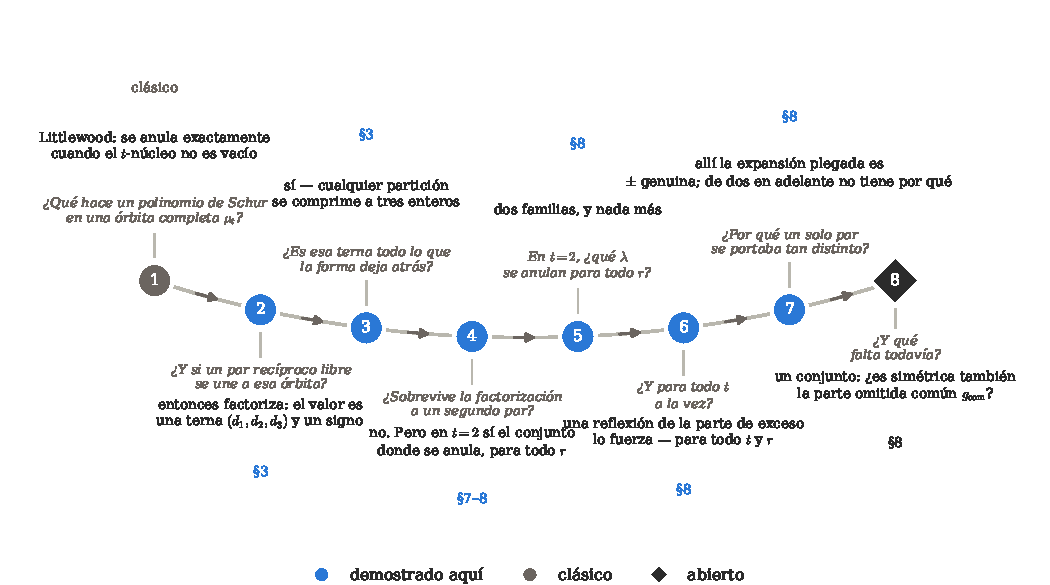
\includegraphics[width=\textwidth]{fig_thread_es.pdf}
\caption{El artículo como un solo hilo. Cada pregunta la responde la perla que tiene debajo, y
cada respuesta es lo que hace que la siguiente pregunta sea la natural: la órbita pide el par
libre, la factorización pide la terna, la terna pide el segundo par, y el segundo par convierte una
fórmula en un lugar. El color distingue lo clásico, lo demostrado aquí y lo que queda abierto, y la
etiqueta bajo cada respuesta es la sección que la resuelve. Dibujada por
\texttt{anc/fig\_intro.py}.}
\label{fig:thread}
\end{figure}

\begin{figure}[!ht]
\centering
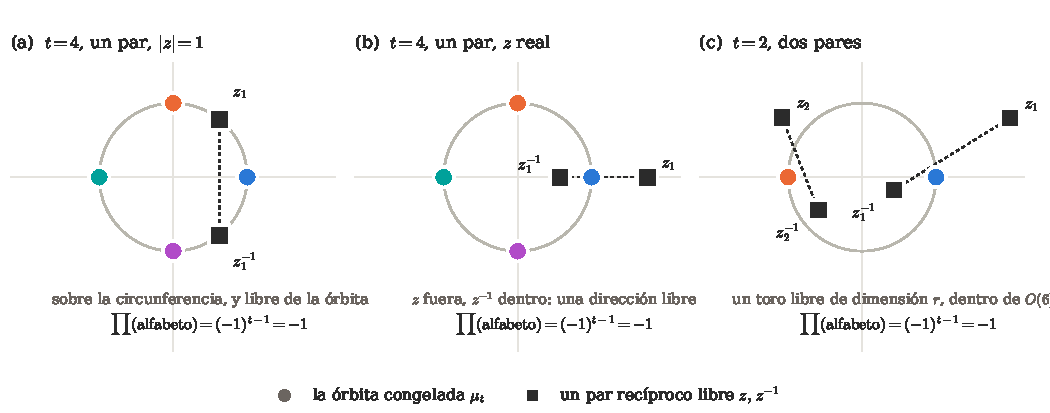
\includegraphics[width=\textwidth]{fig_alphabet_es.pdf}
\caption{El alfabeto, en el plano complejo. La órbita $\mu_t$ está congelada ---un $t$-gono
regular sobre la circunferencia unidad, coloreado por residuo--- y cada par recíproco es una
dirección compleja libre, dibujada unida por un segmento discontinuo. \emph{(a)} el par puede estar
sobre la circunferencia; es una variable libre y no parte de la órbita, y salvo para finitos $z$ no
toca $\mu_t$, que es la razón de que un operador hecho para órbitas de $\zeta$ no tenga nada que
decir de él. \emph{(b)} fuera de la circunferencia, $z$ por fuera y $z^{-1}$ por dentro. \emph{(c)}
$r$ pares dan un toro libre de dimensión $r$. En todos los casos el alfabeto es cerrado por
inversión, así que es la lista de valores propios de un elemento de $O(N,\CC)$ ---el panel (b)
muestra por qué el grupo tiene que ser el complejo--- y el producto de sus letras vale $\zeta^{t(t-1)/2}=(-1)^{t-1}$: para $t$ par esa matriz
está en la componente no identidad. Calculada por \texttt{anc/fig\_intro.py}.}
\label{fig:alphabet}
\end{figure}


Una partición puede ser arbitrariamente grande, y un alfabeto de $N=t+2$ letras sólo alcanza a ver
una parte de ella. Este artículo resuelve, para un alfabeto, exactamente cuánta. El conjunto
completo de las raíces $t$-ésimas de la unidad junto con un par recíproco libre ve un multiconjunto
de tres enteros y un signo, y nada más en absoluto: dos particiones de cualesquiera tamaños que
coincidan en ese dato toman ahí el mismo valor. La forma cerrada del Teorema \ref{thm:main} es cómo
lo demostramos, y la compresión es la parte que esperamos que sobreviva a la fórmula.

La evaluación de polinomios de Schur en raíces de la unidad es clásica y notablemente limpia.
Littlewood y Richardson \cite{LR34} demostraron que $s_\lambda$ se especializa a $0$ o $\pm1$ cuando
las variables se toman como todas las raíces $t$-ésimas de la unidad, siendo el signo un signo de
ordenación y estando la anulación gobernada por el $t$-núcleo de $\lambda$; y en el mismo trabajo lo
generalizaron a un alfabeto que lleva una variable libre en cada letra. Este último resultado fue
redescubierto por Prasad \cite{Pra16}, recibió una nueva demostración de Karmakar \cite{Kar22}, fue
extendido a todos los grupos clásicos por Ayyer y Kumari \cite{AK22} ---quienes además identificaron
el trabajo anterior, casi inadvertido, de Lecouvey \cite{Lec09}--- y fue llevado a los caracteres
universales por Albion \cite{Alb23}. Kumari \cite{Kum24} amplió la familia, Karmakar \cite{Kar24}
trató los elementos de orden dos, Ayyer y Kumari \cite{AK25} añadieron varias especializaciones más,
y Albion \cite{Alb25} relacionó las factorizaciones con las particiones $z$-asimétricas y el
plethysm. Sathish Kumar \cite{SK23} llevó la factorización a las formas sesgadas con
banderas, donde produce una familia de caracteres de Demazure; allí se exige que las banderas
sean múltiplos de $t$, que es la misma demanda de estructura de raíces de la unidad con otro
disfraz. Leída en conjunto, esa línea hace algo más que acumular casos. El enunciado migra de un
grupo a un alfabeto: una vez que los caracteres son universales, evaluar uno es una pregunta sobre
qué letras se escriben, y los tipos clásicos dejan de ser teoremas separados ---el Teorema 5.3 de
\cite{AK25} es un solo enunciado para $s$, $sp$ y $o$ a la vez---. Esa migración es lo que vuelve
formulable la pregunta de este artículo, porque el alfabeto de abajo no pertenece a ningún grupo de
la lista; y las herramientas que tomamos prestadas en la \S\ref{sec:zeros} son las que esa migración
produjo. Remitimos a Albion \cite{Alb23} para un recorrido de toda la línea.

Leído por su \emph{valor}, el teorema de Littlewood es una factorización. Leído por sus \emph{ceros}
es otra cosa ---una clasificación de las $\lambda$ que mueren en un elemento de orden $t$--- y esa
segunda lectura tiene un descendiente propio, que conviene nombrar aquí porque la
\S\ref{sec:zeros} resulta ser su prima. Prasad \cite[Teorema 2]{Pra16} plantea la pregunta de la
anulación no en un punto sino a lo largo de toda una familia: sobre la componente no identidad de
$GL_m^n\rtimes\ZZ/n$ determina cuándo el carácter es idénticamente cero \emph{como función del
parámetro libre}, y la respuesta se lee otra vez en las clases de residuos de $\lambda+\delta$
---cada clase tiene que estar representada exactamente $m$ veces---. En $m=1$ eso es la condición de
Littlewood. Así que un teorema de 1934 tiene dos descendientes, y se separan en qué se permite
que siga libre: allí, órbitas completas de raíces de la unidad; aquí, como veremos, una sola órbita
congelada junto con direcciones \emph{recíprocas} libres. Ninguno de los dos enunciados contiene al
otro.

Una segunda línea de resultados de factorización trata alfabetos cerrados bajo $x\mapsto x^{-1}$.
Okada \cite{Oka98} y Ciucu--Krattenthaler \cite{CK09} trataron las formas rectangulares; Behrend,
Fischer y Konvalinka, y Ayyer, Behrend y Fischer, las escaleras dobles ---para las que seguimos las
atribuciones que da \cite{AB19}---; y Ayyer--Behrend \cite{AB19} las formas autoduales, con
demostraciones biyectivas de estas últimas debidas a Ayyer y Fischer \cite{AF20}. Allí el rédito es
enumerativo: las factorizaciones producen fórmulas de producto para clases de simetría de particiones
planas y para teselaciones de rombos. Las formas autocomplementarias de \cite{AB19} reaparecen en la
\S\ref{sec:zeros} por el otro lado: añadir la letra $-1$ cambia el determinante del alfabeto de $+1$
a $-1$, y las formas que allí factorizan son exactamente las que aquí se anulan.

Las dos líneas nunca han compartido alfabeto, y el obstáculo es estructural en ambas direcciones. El
motor de la primera es un operador ---la Verschiebung $\varphi_t$, en la formulación de Albion
\cite{Alb23}, que actúa sobre los caracteres universales por $\varphi_t h_r=h_{r/t}$ si $t\mid r$ y
$0$ en otro caso--- que exige que el alfabeto sea unión de $\zeta$-órbitas; toda extensión de esa
línea añade por tanto \emph{más} estructura de raíces de la unidad, nunca menos. El motor de la
segunda exige que el alfabeto sea enteramente recíproco, o que la forma sea autocomplementaria. Un
par recíproco libre no es una $\zeta$-órbita, y una órbita de raíces de la unidad no es unión de
pares libres.

La palabra \emph{más pequeño} de abajo puede precisarse, y es el cierre por inversión quien lo
permite. Una extensión de $\zt$ cerrada por inversión solo puede adjuntar pares recíprocos
$\{x,x^{-1}\}$ y los puntos fijos de la inversión, que son $1$ y $-1$; ahora bien, $1$ está en $\zt$
para todo $t$, y $-1$ está en $\zt$ exactamente cuando $t$ es par. La única extensión menor que un
par es por tanto $\zt\cup\{-1\}$ con $t$ impar, y está congelada: sobre $t=3,5,7$ y
$|\lambda|\le14$, las $1092$ formas, $s_\lambda(\zt,-1)$ solo toma los valores $0$ y $\pm1$, sin
nada de lo que pueda depender. Un par recíproco libre es la extensión más pequeña que deja algo que
evaluar.

En este artículo tomamos el alfabeto más pequeño que contiene una letra de cada clase,
\begin{equation}\label{eq:object}
\Phi_t(\lambda;z)\;:=\;s_\lambda\bigl(\,\underbrace{1,\zeta,\dots,\zeta^{t-1}}_{\zt},\;z,\;z^{-1}\bigr),
\qquad \zeta=e^{2\pi i/t},
\end{equation}
un polinomio de Schur en $N=t+2$ variables.

Descrito así, \eqref{eq:object} es un compromiso entre dos líneas, que es como lo encontramos. Se
describe mejor como un solo objeto, y esa descripción es la que reaparece en cada sección de abajo:
\eqref{eq:object} es \emph{un elemento del toro de $O(N)$ con una única dirección libre}. Es cerrado
por inversión, de modo que ya vive donde vive la segunda línea; su determinante es $(-1)^{t+1}$, y
ese determinante es lo que separa factorizar de anularse en la \S\ref{sec:zeros}; la $\zeta$-órbita
es lo que lo coloca en la componente no identidad cuando $t$ es par, donde un carácter es un carácter
entrelazado, que es la Observación \ref{rem:twining}; y el único par libre es la única variable que
sobrevive a la enumeración con signo de la \S\ref{sec:enum}. Los tres resultados de este artículo son
tres lecturas de esa frase.

Nuestro resultado principal, el Teorema \ref{thm:main},
lo evalúa para todo $t$ y toda $\lambda\in\PP_N$ ---toda partición con a lo sumo $N$ partes, sin
restricción alguna sobre su forma ni su tamaño---. Escribimos $\beta=\beta(\lambda,N)$ para la partición
desplazada y $n_i(\lambda)$ para el número de partes de $\beta$ congruentes con $i$ módulo $t$, como
en \cite{AK22}. Puesto que hay $t$ clases de residuos y $N=t+2$ partes, $\sum_i(n_i-1)=2$; luego o
alguna clase está vacía, o, estando todas ocupadas, el exceso sobre una cada una es exactamente dos,
y solo se dan tres perfiles: algún $n_i$ se anula, o dos clases tienen tamaño dos, o una clase tiene
tamaño tres. En el primer caso $\Phi_t=0$; en los otros dos, si $A=\{a_1>a_2\}$ y $B=\{b_1>b_2\}$
denotan las dos clases distinguidas y
\[
d_1=a_1-a_2,\qquad d_2=b_1-b_2,\qquad
\tilde d_3=a_1+a_2-b_1-b_2,\qquad d_3=|\tilde d_3| ,
\]
entonces $\Phi_t=0$ si el \emph{acoplamiento orientado} $\tilde d_3$ se anula, y en otro caso, con
$z=e^{\theta}$,
\[
\boxed{\;\;\Phi_t(\lambda;z)\;=\;\varepsilon_\lambda\,
\frac{\sinh(d_1\theta/2)\,\sinh(d_2\theta/2)\,\sinh(d_3\theta/2)}
{\sinh^2(t\theta/2)\,\sinh\theta}\;\;}
\]
con $\varepsilon_\lambda=\pm1$ dado explícitamente. \emph{Tres factores, nunca más, y sin ninguna
hipótesis sobre la forma de $\lambda$.} Retirado el par recíproco, el enunciado degenera en el de
Littlewood, de modo que el contenido es lo que ese par añade: exactamente un término de
acoplamiento, a saber $d_3$. Leído con caracteres $\mathfrak{sl}_2$ el mismo enunciado no lleva
exponencial ninguna: es el producto triple $\chi_{d_1/2-1}\chi_{d_2/2-1}\chi_{d_3/2-1}$ sobre
$\chi_{t/2-1}^2$, uniformemente en $t$ (Corolario \ref{cor:chars}), con índices semienteros
exactamente cuando $t$ es impar.

El alfabeto es un solo objeto, y la respuesta también. El perfil de residuos, la terna
$(d_1,d_2,d_3)$ y el signo son todo lo que el teorema necesita, y en la \S\ref{sec:main} los
reunimos en un único \emph{invariante de la evaluación} $I_t(\lambda)$, \eqref{eq:invariant}, a
través del cual el valor factoriza. Es completo pero no mínimo: \eqref{eq:main} es simétrica en los
tres enteros, de modo que lo que se ve es el multiconjunto y el signo, que es la compresión
anunciada arriba. Lo que \emph{no} se ve es entonces una pregunta bien planteada. La
\S\ref{sec:fibrelattice} la responde para los tres enteros ---las particiones que los comparten
forman un retículo, y escribimos su función generatriz--- y lo que el signo añade a eso es el
Problema \ref{prob:fibres}.

Los tres enteros admiten una lectura que vuelve transparente la fórmula, y la damos aquí porque es
como pensamos el resultado. Considérense $A$ y $B$ como intervalos $[a_2,a_1]$ y $[b_2,b_1]$ sobre la
recta beta. Entonces
\begin{equation}\label{eq:intervals}
d_1=|A|,\qquad d_2=|B|,\qquad d_3=2\,\bigl|\mathrm{centro}(A)-\mathrm{centro}(B)\bigr| :
\end{equation}
\emph{las dos longitudes, y el doble de la distancia entre los centros} (Figura
\ref{fig:intervals}). El criterio de anulación se vuelve geométrico ---una clase de residuos es
vacía, o los dos intervalos son concéntricos--- y explica de inmediato por qué el perfil de tamaño
tres, donde los intervalos comparten un extremo, nunca se anula. Los intervalos concéntricos
resultan exigir $t$ par (Proposición \ref{rem:lattice}), de modo que para $t$ impar una clase de
residuos vacía es la única forma de anularse ---y eso sigue siendo cierto para cualquier número de
pares recíprocos, que es el Corolario \ref{cor:oddgen}---. Equivalentemente, en el idioma de la
primera línea, $d_1$ y $d_2$ son $t$ veces los contenidos $\mathfrak{sl}_2$ de las dos componentes
distinguidas del cociente, y el acoplamiento orientado $\tilde d_3$ es un funcional \emph{afín} sobre
el vector de \emph{tamaños} del cociente, entrando los dos residuos como un desplazamiento, con
$d_3=|\tilde d_3|$ (Proposición \ref{prop:quotient}). No es
un funcional sobre el vector de residuos, y por tanto tampoco sobre el retículo de raíces de tipo
$A_{t-1}$ bajo la correspondencia de Garvan--Kim--Stanton \cite{GKS90}: ya en $t=2$ el único perfil
de dos clases lleva diez valores distintos de $d_3$ sobre $|\lambda|\le16$. En qué mitad de la
descomposición núcleo--cociente vive cada cláusula del criterio de anulación queda resuelto en la
Proposición \ref{rem:lattice}.

Se siguen dos consecuencias. El Teorema 5.3 de \cite{AK25} determina cuándo un carácter universal es
independiente de las variables por las que se le tuerce, uniformemente en los tres tipos clásicos, y
leído sobre \eqref{eq:object} diría que
$s_\lambda(z,z^{-1},\zt)=s_\lambda(z,z^{-1})$ exactamente sobre los $t$-núcleos, para
$\ell(\lambda)\le2$. Ese criterio está enunciado para variables libres, y un par recíproco no lo es;
sobre ese lugar aparece una familia más, y el Teorema \ref{thm:extra} la clasifica por su núcleo y su cociente. En
\S\ref{sec:enum} leemos la identidad como una enumeración: una fórmula de producto para un recuento
de tablas semiestándar pesado por raíces de la unidad en el que el parámetro $z$ sigue libre, y en
$t=2$ una $(-1)$-enumeración de particiones planas en una caja refinada por $z$.

Las dos últimas secciones hacen una pregunta distinta, no sobre lo que la identidad da sino sobre
hasta dónde alcanza. La \S\ref{sec:sharp} prueba cuatro deformaciones naturales del alfabeto, cada
una de las cuales destruye la identidad, y una sola lectura de la demostración explica las
cuatro. Luego la
\S\ref{sec:zeros} aísla lo que sí sobrevive. Añadir más pares recíprocos cuesta la fórmula de
producto del Teorema \ref{thm:main}, pero
no el \emph{lugar de anulación}: para todo número $r$ de pares, el carácter
$s_\lambda(1,-1,z_1,\bar z_1,\dots,z_r,\bar z_r)$ se anula exactamente cuando el conjunto beta tiene
paridad constante o $\lambda$ es autocomplementaria de anchura impar (Teorema \ref{conj:crit}).
Leído sobre el grupo y no sobre el alfabeto, el mismo enunciado es una clasificación: ésas son
exactamente las $\lambda$ cuyo $GL(N)$-módulo restringe a $O(N)$ de forma estable bajo el giro por
$\det$ (Corolario \ref{cor:dettwist}). Las formas son las autocomplementarias de \cite{AB19}, donde el mismo
alfabeto sin la letra $-1$ hace que el carácter factorice en lugar de anularse; el determinante del
alfabeto decide cuál de las dos cosas pasa. La dirección suficiente es un corolario corto de la
complementación y lo decimos así; el contenido es el recíproco, que demostramos para todo $r$ y toda
$\lambda$, módulo un teorema de rigidez para productos de polinomios de Schur.

Conviene dibujar el mapa, y la Figura \ref{fig:plane} lo es. Adjuntar $r$ pares recíprocos a la
órbita $\zt$ da una familia en los dos parámetros $(t,r)$, y el lugar de anulación está resuelto en
tres partes de ella --- una fila, una columna, y todas las columnas impares, que son medio plano.

\begin{figure}[!ht]
\centering
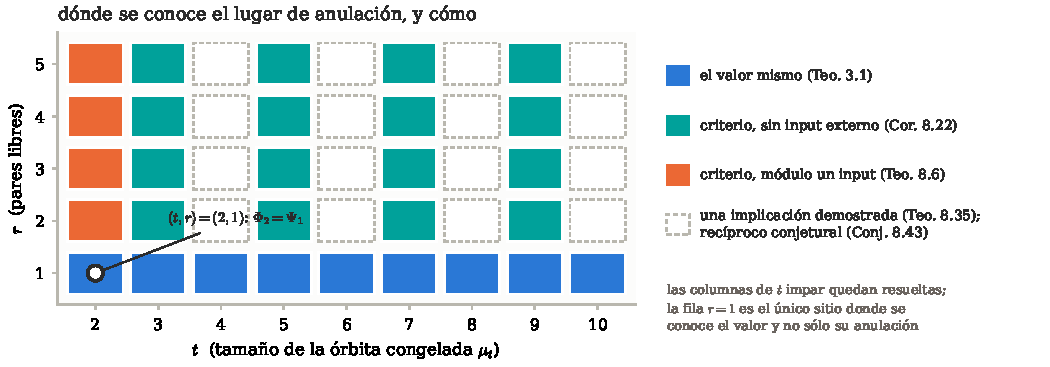
\includegraphics[width=\textwidth]{fig_plane_es.pdf}
\caption{La familia de dos parámetros, y lo que se sabe sobre ella. Cada celda es un alfabeto
$\zt\cup\{z_1^{\pm1},\dots,z_r^{\pm1}\}$; el color no se asigna a mano, sino que se calcula a partir
de los propios enunciados, con una regla por línea del artículo. La fila $r=1$ es el único sitio
donde se conoce el \emph{valor} y no sólo su anulación, que es el Teorema \ref{thm:main}; las
columnas de $t$ impar las resuelve el Corolario \ref{cor:oddgen} sin ningún input externo; la columna
$t=2$, el Teorema \ref{conj:crit}, que usa uno. En las celdas restantes el Teorema \ref{thm:suff}
prueba una implicación y la Conjetura \ref{conj:general} es la otra. La esquina marcada es donde se
encuentran las dos mitades del artículo: allí $\Phi_2=\Psi_1$, y es el único alfabeto que ven las
dos. Calculada por \texttt{anc/fig\_plane.py}.}
\label{fig:plane}
\end{figure} El Teorema \ref{thm:main}
es $r=1$: un par, todo $t$, y ahí tenemos el valor y no sólo su anulación.
El Teorema \ref{conj:crit} es $t=2$: cualquier número de pares, la órbita más pequeña. Y el Corolario
\ref{cor:oddgen} es \emph{todo $t$ impar y todo $r$} a la vez: allí el carácter se anula si y sólo si
falta una clase de residuos, de modo que la rama concéntrica es un fenómeno exclusivo de $t$ par. La
tercera de las tres no es un borde sino medio plano, y es además la más barata --- sale del argumento
extremal de la \S\ref{sec:extremal} sin ningún input externo, mientras que la segunda necesita el
Teorema \ref{thm:PvW}. Fuera de esas tres regiones el lugar no está resuelto, pero ya no está intacto. El
Teorema \ref{thm:suff} da una condición sobre el conjunto beta --- una reflexión de su parte de
exceso, y un incremento que da en el centro --- que fuerza la anulación del carácter para
\emph{todo} $t$ y todo $r$, mediante una involución que empareja todos los términos del desarrollo;
el Corolario \ref{cor:necgen} da una condición necesaria por el otro lado. Que las dos se encuentren
es la Conjetura \ref{conj:general}, y lo que las separa es una sola implicación, que la
\S\ref{sec:rigidity} muestra que no puede venir del estrato en el que ese argumento trabaja. El
fórmula de producto del Teorema \ref{thm:main} ya falla en $r=2$, por (D1) ---que no exista tal
fórmula para ningún $r\ge2$ es la Conjetura \ref{conj:rank2}, y no algo que demostremos---, así que
pasada la línea $r=1$ el lugar es lo que podemos ofrecer.

Hay algo que el alfabeto delata y que merece decirse aquí y no de pasada. Tiene una lectura en
teoría de representaciones ---de la clase que \cite{CK09} registran como ausente para sus
factorizaciones, y con ellos \cite{AB19} y \cite{AK25}--- y el mecanismo no es nuestro: el alfabeto
es cerrado por inversión, luego
un elemento del toro de $O(N)$ de determinante $(-1)^{t+1}$, de modo que para $t$ par vive en la
componente no identidad, donde un carácter es un carácter \emph{entrelazado} en el sentido de
Jantzen \cite{Jantzen} y Kumar--Lusztig--Prasad \cite{KLP} y el plegado lo da el álgebra de Lie de
órbitas. La Observación \ref{rem:twining} lo precisa y el Lema \ref{lem:AtoSp} lo concreta ---allí el
álgebra plegada es $C_r$ y el carácter entrelazado es un carácter simpléctico sin más. La
demostración del Teorema \ref{thm:main} no usa nada de eso, y por eso lo enunciamos como lectura y no
como método.

El artículo se organiza como sigue. Fijamos notación y recordamos las dos evaluaciones sobre las que
construimos en la Sección \ref{sec:background}. En la Sección \ref{sec:main} enunciamos el teorema
principal, identificamos sus tres enteros en términos del núcleo y del $t$-cociente, describimos las
particiones que no consiguen separar y registramos el criterio de
anulación y la imagen de la aplicación resultante. La Sección \ref{sec:proof} contiene la
demostración. En la Sección \ref{sec:independence} comparamos el teorema con el criterio de
independencia de \cite{AK25} y determinamos la familia adicional que adquiere en el lugar recíproco.
En la Sección \ref{sec:enum} leemos el teorema como una enumeración y ensamblamos, en $t=2$, la
involución que invierte el signo que esa enumeración pide, y en la Sección
\ref{sec:sharp} probamos cuatro deformaciones del alfabeto, cada una de las cuales destruye la
identidad. La Sección \ref{sec:zeros} determina
el lugar de anulación en $t=2$ para un número arbitrario de pares recíprocos ---y, sin ningún coste
externo, también en todo $t$ impar---, lee ese criterio sobre el grupo como una rigidez frente al
giro por el determinante, y da un criterio suficiente, con recíproco conjetural, para $t$ y $r$
arbitrarios. La Sección \ref{sec:verif} recoge las
comprobaciones numéricas y la Sección \ref{sec:open} los problemas abiertos.

%======================================================================
\section{Preliminares y notación}\label{sec:background}

Seguimos la notación de \cite{AK22,AK25}. Todos los grupos algebraicos son aquí sobre $\CC$; en
particular $O(N)$ significa $O(N,\CC)$, que es lo que da un alfabeto cerrado por $x\mapsto x^{-1}$
cuando se permite a sus letras salir de la circunferencia unidad.

\subsection{Particiones, conjuntos beta, núcleos y cocientes}
Una partición $\lambda=(\lambda_1,\dots,\lambda_n)$ es una sucesión débilmente decreciente de enteros
no negativos; $\PP_n$ denota el conjunto de particiones de longitud a lo sumo $n$, $|\lambda|$ el
tamaño y $\ell(\lambda)$ la longitud. En todo el texto $t\ge2$ es un entero fijo, $\zeta$ una raíz
$t$-ésima primitiva de la unidad, $\zt=\{1,\zeta,\dots,\zeta^{t-1}\}$, y
\[
N:=t+2 .
\]
Para $\lambda\in\PP_N$ el \emph{conjunto beta} es $\beta(\lambda)=(\beta_1,\dots,\beta_N)$ con
$\beta_j=\lambda_j+N-j$, de modo que $\beta_1>\beta_2>\dots>\beta_N\ge0$; indexamos por
\emph{columnas} $j=1,\dots,N$, y observamos que un $\beta$ mayor significa un índice de columna menor.
Para $0\le i\le t-1$ escribimos $n_i(\lambda)$ para el número de partes de $\beta(\lambda)$
congruentes con $i$ módulo $t$, de manera que
\begin{equation}\label{eq:excess}
\sum_{i=0}^{t-1}n_i(\lambda)=N=t+2 .
\end{equation}
Llamamos \emph{perfil de residuos} de $\lambda$ al vector
$\bigl(n_0(\lambda),\dots,n_{t-1}(\lambda)\bigr)$. Por \eqref{eq:excess},
$\sum_i\bigl(n_i(\lambda)-1\bigr)=2$: o alguna clase está vacía, o, estando todas ocupadas, el
exceso sobre una cada una es exactamente dos, y sólo hay dos particiones de dos. De modo que un
perfil es de exactamente uno de tres tipos: \emph{degenerado}, si algún $n_i=0$; \emph{de dos
clases}, si dos entradas valen $2$; o \emph{de tamaño tres}, si una entrada vale $3$. Todo lo que
sigue en este artículo está gobernado por cuál de los tres se da.
Sea $\sigma\in S_N$ la permutación que reordena las partes de $\beta(\lambda)$ agrupándolas por clase
de residuo, con las clases en orden creciente y los valores dentro de cada clase en orden
decreciente; es la permutación de \cite[(2.1)]{AK25}. Escribimos $\core_t(\lambda)$ y
$\quot_t(\lambda)=(\lambda^{(0)},\dots,\lambda^{(t-1)})$ para el $t$-núcleo y el $t$-cociente,
definidos a partir de $\beta(\lambda)$ como en \cite[\S2.1]{AK25}. Por \cite{GKS90}, los $t$-núcleos
están en biyección con los vectores del retículo de raíces de tipo $A_{t-1}$, y los recuentos de
residuos $n_i$ son las coordenadas naturales.

Ponemos $\zb:=z^{-1}$, $z=e^{\theta}$, y abreviamos
\[
f(u):=z^{u}-z^{-u}=2\sinh(u\theta),\qquad
V:=\prod_{0\le k<k'\le t-1}\bigl(\zeta^{k'}-\zeta^{k}\bigr).
\]
Para un conjunto $S$ de columnas, $b_S$ es la palabra de residuos $\beta_j\bmod t$ para $j\in S$
leída en orden creciente de columna, e $\inv(b_S)$ su número de inversiones. Usamos el bialternante
\[
s_\lambda(x_1,\dots,x_N)=\frac{\det\bigl(x_i^{\beta_j}\bigr)_{i,j=1}^N}
{\det\bigl(x_i^{N-j}\bigr)_{i,j=1}^N}.
\]

\subsection{Las dos evaluaciones sobre las que construimos}
Recordamos los dos enunciados entre los que se sitúa el presente resultado. El primero es la
evaluación de Littlewood, en la forma de \cite[Teorema 2.2]{AK25}.

\begin{theorem}[{\cite[Teorema IX]{LR34}}]\label{thm:LR}
Sea $\lambda\in\PP_t$. Entonces
\[
s_\lambda(1,\zeta,\dots,\zeta^{t-1})=
\begin{cases}
(-1)^{\binom{t}{2}}\sgn(\sigma) & \text{si }\core_t(\lambda)=\varnothing,\\
0 & \text{en otro caso.}
\end{cases}
\]
\end{theorem}

El segundo es el criterio de independencia que extendemos, \cite[Teorema 5.3]{AK25}; enunciamos el
caso que necesitamos. Sea $f_\lambda$ un carácter universal de tipo $s$, $sp$ u $o$, sea $Y$ un
conjunto de $m$ variables y sean $x_1,\dots,x_{n-tm}$ libres. Entonces
\begin{equation}\label{eq:AK53}
f_\lambda(x_1,\dots,x_{n-tm},Y,\zeta Y,\dots,\zeta^{t-1}Y)=f_\lambda(x_1,\dots,x_{n-tm})
\quad\Longleftrightarrow\quad \lambda=\core_t(\lambda),
\end{equation}
para $\lambda\in\PP_{n-tm}$. El criterio es uniforme en el tipo ---un solo enunciado para $s$, $sp$ y
$o$ a la vez---, que es lo que lo hace citable aquí: nuestro alfabeto es un alfabeto de $GL$, y lo
que le preguntamos es una cuestión sobre una especialización y no sobre un grupo. Tomando $m=1$,
$Y=(1)$ y $(x_1,x_2)=(z,\zb)$ se obtiene $n=t+2$ y nuestro alfabeto, pero esa sustitución es
justamente donde se abandona la hipótesis de que $x_1,x_2$ sean libres. Así que \eqref{eq:AK53} no se
está aplicando sobre el lugar recíproco; se le está preguntando por él, que es la
\S\ref{sec:independence}.

\begin{remark}\label{rem:notacase}
El enunciado más próximo de la literatura añade dos letras extra, igual que nosotros, de modo que
conviene registrar por qué no contiene \eqref{eq:object}. Kumari \cite[Teorema 2.2]{Kum24} evalúa
$s_\lambda(X,\zeta X,\dots,\zeta^{t-1}X,\,y,\zeta y,\dots,\zeta^{m-1}y)$; con $X=(1)$ y $m=2$ el
bloque añadido es $\{y,\zeta y\}$, mientras que el nuestro es $\{z,z^{-1}\}$. Los dos coinciden solo
cuando $z^{2}=\zeta^{\pm1}$, un conjunto finito de puntos y no una variable libre. Lo mismo vale para
la única variable libre extra de \cite[Teorema 2.7]{AK22} y para el Teorema XI de
Littlewood--Richardson.
\end{remark}

%======================================================================
La Figura \ref{fig:beta} hace todo el diccionario sobre una forma concreta.

\begin{figure}[!ht]
\centering
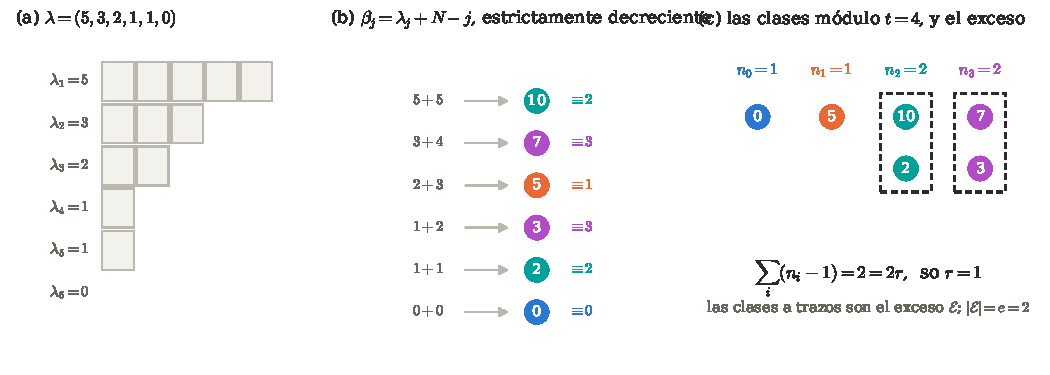
\includegraphics[width=\textwidth]{fig_beta_es.pdf}
\caption{El diccionario sobre el que corre el resto del artículo, con $\lambda=(5,3,2,1,1,0)$ y
$t=4$. \emph{(a)} la forma, rellenada hasta $N$ partes. \emph{(b)} $\beta_j=\lambda_j+N-j$, que
convierte una sucesión débilmente decreciente en una estrictamente decreciente y por tanto en un
conjunto; cada valor se colorea después según su residuo módulo $t$. \emph{(c)} el perfil de
residuos $(n_0,\dots,n_{t-1})$ y el recuento \eqref{eq:excess}: $\sum_i(n_i-1)=2r$ siempre, de modo
que cuando toda clase está ocupada las clases con $n_i\ge2$ ---el exceso $\mathcal{E}$, a trazos---
llevan exactamente $2r$ elementos más de uno cada una. Si alguna está vacía la suma sigue valiendo
$2r$ pero ya no es un exceso: ésa es la rama degenerada, que se resuelve la primera.
Todo lo que el artículo demuestra es un enunciado sobre ese dibujo.
Calculada por \texttt{anc/fig\_intro.py}.}
\label{fig:beta}
\end{figure}

\section{La evaluación}\label{sec:main}

\keybox{\emph{El teorema en una frase.} El valor depende de $\lambda$ a través de su perfil de
residuos, una terna de intervalos $(d_1,d_2,d_3)$ y un signo, y de nada más: una partición
arbitrariamente grande queda comprimida a tres enteros y un signo.}

\begin{theorem}\label{thm:main}
Sean $t\ge2$ y $\lambda\in\PP_N$, con $N=t+2$.
\begin{enumerate}
\item[\rm(i)] Si $n_i(\lambda)=0$ para algún $i$, entonces $\Phi_t(\lambda;z)=0$.
\item[\rm(ii)] En caso contrario, por \eqref{eq:excess}, o bien exactamente dos clases de residuos
tienen $n_i=2$, o bien exactamente una tiene $n_i=3$. Sean $r_A\le r_B$ los residuos implicados y
sean
\[
A=\{a_1>a_2\},\qquad B=\{b_1>b_2\}
\]
en el primer caso las partes de $\beta(\lambda)$ en las clases $r_A$ y $r_B$, y en el segundo los dos
pares solapados $A=\{p,q\}$, $B=\{q,r\}$ de la clase $\{p>q>r\}$, de modo que $r_A=r_B$. Pongamos
\[
d_1=a_1-a_2,\qquad d_2=b_1-b_2,\qquad
\tilde d_3=a_1+a_2-b_1-b_2,\qquad d_3=|\tilde d_3| ,
\]
y llamemos a $\tilde d_3$ el \emph{acoplamiento orientado}. Si $\tilde d_3=0$, entonces
$\Phi_t(\lambda;z)=0$. En caso contrario, con $z=e^\theta$,
\begin{equation}\label{eq:main}
\boxed{\;\;\Phi_t(\lambda;z)\;=\;\varepsilon_\lambda\cdot
\frac{\sinh(d_1\theta/2)\,\sinh(d_2\theta/2)\,\sinh(d_3\theta/2)}
{\sinh^2(t\theta/2)\,\sinh\theta}\;\;}
\end{equation}
donde, escribiendo $j_{A_1}$ y $j_{B_1}$ para las columnas que llevan $a_1$ y $b_1$, $S$ para el
complementario de $\{j_{A_1},j_{B_1}\}$ en $\{1,\dots,N\}$, y $b_S$ para la palabra de residuos de
$\beta(\lambda)$ sobre $S$ leída en orden creciente de columna,
\begin{equation}\label{eq:sign}
\varepsilon_\lambda\;=\;(-1)^{\,t+\binom{N+1}{2}}\;
(-1)^{\,j_{A_1}+j_{B_1}+\inv(b_S)}\;\sgn(a_1-b_1)\;\sgn(\tilde d_3).
\end{equation}
\end{enumerate}
Cada uno de los cuatro factores es $\pm1$ ---el último porque $\tilde d_3\ne0$ es exactamente la
hipótesis de {\rm(ii)}---, luego $\varepsilon_\lambda=\pm1$. En el perfil de tamaño tres $r_A=r_B$ y
$\tilde d_3=p-r>0$, luego ese factor es $+1$.

El lado izquierdo es un polinomio de Laurent en $z$. Leemos \eqref{eq:main} como identidad en
$\CC(z)$; tras la cancelación el lado derecho es también un polinomio de Laurent, y en los ceros del
denominador ---$z=\pm1$ y $z^t=1$--- usamos esa continuación. Así lo hacemos en \S\ref{sec:enum},
donde el valor se toma en $z=1$.
\end{theorem}

\noindent Separar $d_3$ en su tamaño y su orientación no es contabilidad. El signo \eqref{eq:sign}
necesita la orientación y la fórmula necesita solo el tamaño, y en $\tilde d_3=0$ la orientación no
existe: un enunciado que lleve $\sgn(a_1+a_2-b_1-b_2)$ y afirme que vale $\pm1$ es falso sobre el
lugar concéntrico, donde ese argumento es cero. El valor allí es $0$ por el factor
$\sinh(d_3\theta/2)$, de modo que nada de lo que viene después cambia; lo que cambia es que el caso
queda ahora excluido antes de escribir el signo, y no después.

Escribimos
\[
d(\lambda):=(d_1,d_2,d_3)
\]
y lo llamamos la \emph{terna de intervalos} de $\lambda$, siguiendo la lectura
\eqref{eq:intervals}; y llamamos a $d_3$ el \emph{término de acoplamiento}, por ser el único de los
tres que mezcla las dos clases distinguidas.

Conviene dar nombre al dato completo, porque el teorema se lee mejor como un enunciado sobre él que
como una fórmula. Pongamos
\begin{equation}\label{eq:invariant}
\boxed{\;\;I_t(\lambda)\;:=\;\begin{cases}
0 & \text{si el perfil de residuos es degenerado, o }\tilde d_3=0,\\[2pt]
\bigl(d_1,d_2,d_3,\varepsilon_\lambda\bigr) & \text{en otro caso},
\end{cases}\;\;}
\end{equation}
y llamémoslo el \emph{invariante de la evaluación} de $\lambda$. Su primera rama es exactamente el
lugar de anulación del Corolario \ref{cor:zero}, y es una rama y no dos porque en todo él no hay
signo que registrar: \eqref{eq:sign} necesita $\tilde d_3\ne0$. El Teorema \ref{thm:main} dice
entonces dos cosas a la vez. Primera, que $\Phi_t$ \emph{factoriza a través} de $I_t$: la aplicación
$\lambda\mapsto\Phi_t(\lambda;z)$ es la composición de $\lambda\mapsto I_t(\lambda)$ con una función
del invariante solo. Segunda, que ese invariante es \emph{completo} para esta evaluación: si dos
particiones tienen el mismo $I_t$ tienen el mismo $\Phi_t$, sean del tamaño que sean. La completitud
es lo que hace que la compresión anunciada más arriba merezca un nombre y no solo una observación
---dice que el invariante no es un resumen cómodo de la dependencia, sino la dependencia entera--- y
convierte la pregunta natural siguiente, qué olvida el invariante, en una pregunta bien planteada.
La Proposición \ref{prop:minimal} cierra la pregunta por el otro lado: una vez leída la terna como
multiconjunto, tampoco puede suprimirse nada de $I_t$. Así que la \S\ref{sec:fibrelattice} resuelve
qué se olvida para la terna y el Problema \ref{prob:fibres} es lo que deja
el signo. Los $(d_1,d_2,d_3)$ de la Figura \ref{fig:image} son
los valores que toma este invariante, dibujados.

Esa factorización es una sola tubería, y cada flecha pierde información que ya no vuelve:
% multline y no \[...\]: la cadena entera no cabe en una caja de 436 pt, y una formula sin puntos
% de corte no se parte sola.  El corte va tras el paso que pierde los intervalos, que es donde el
% lector para de todos modos.
\begin{multline*}
\lambda\;\longrightarrow\;\beta(\lambda)\;\longrightarrow\;
\bigl(\text{perfil de residuos},\ \text{los dos intervalos distinguidos}\bigr)\\
\longrightarrow\;\bigl(d_1,d_2,d_3,\varepsilon_\lambda\bigr)\;\longrightarrow\;\Phi_t(\lambda;z).
\end{multline*}
Los intervalos hay que llevarlos junto al perfil: el perfil dice qué clases son las distinguidas y
nada sobre dónde caen sus números beta, de modo que no determina la terna.
Coordenada a coordenada, el invariante reparte el trabajo así.

\begin{center}\small
\begin{tabular}{ll}
\toprule
dato de $\lambda$ & qué controla\\
\midrule
perfil de residuos & la rama degenerada de anulación\\
las dos longitudes $d_1,d_2$ & los dos primeros factores\\
la distancia entre los centros, $d_3$ & el factor de acoplamiento, y la rama concéntrica de anulación\\
la orientación $\sgn(\tilde d_3)$ & un factor del signo\\
el signo de ordenación $\varepsilon_\lambda$ & el signo global\\
\bottomrule
\end{tabular}
\end{center}

\noindent Ninguna de las dos ramas de anulación es la otra: el perfil no puede ver la concéntrica, y
la terna no puede ver la degenerada, y por eso el criterio del Corolario \ref{cor:zero} tiene dos
cláusulas y la \S\ref{sec:main} dedica una proposición a decir dónde vive cada una.

\keybox{Un solo recuento recorre el artículo. Con $t$ clases de residuos, $N=t+2$ partes y toda
clase ocupada, el exceso es exactamente dos, de modo que por \eqref{eq:excess} un perfil sólo
puede ser degenerado, de dos
clases o de tamaño tres: esa tricotomía es la forma del Teorema \ref{thm:main}, la
división en casos de su demostración en la \S\ref{sec:proof}, y la primera rama del lugar de
anulación en la \S\ref{sec:zeros}. Dos clases distinguidas son lo que el par recíproco tiene que
acoplar, y de ahí exactamente un término de acoplamiento y tres factores en vez de dos.}

El recuento de tres tiene una segunda explicación, que no debe nada a la demostración. El exceso
dos da dos clases distinguidas, que son dos intervalos sobre la recta beta, y un par de intervalos
son cuatro números $(a_1,a_2,b_1,b_2)$. Los tres argumentos de \eqref{eq:main} ven qué forma tiene
ese par y no dónde está: un desplazamiento común $\beta\mapsto\beta+m$ deja $d_1$, $d_2$ y
$\tilde d_3$ intactos. Así que lo único que puede entrar en ellos es un funcional lineal que mate la
traslación común, y esos forman el hiperplano $\sum\alpha_i=0$ del dual de dimensión cuatro: un
espacio de dimensión exactamente \emph{tres}. La terna $d_1=(1,-1,0,0)$, $d_2=(0,0,1,-1)$ y
$\tilde d_3=(1,1,-1,-1)$ es una base de él. Módulo la traslación común, un par de intervalos tiene
tres coordenadas lineales independientes, y de ahí sale el recuento de tres. Lo que el Teorema
\ref{thm:main} añade, y que el recuento de dimensiones \emph{no} fuerza, es que en esta
especialización esas tres coordenadas \emph{se separan multiplicativamente}: un producto con un
factor de cada una, y no otra función de tres variables.

El \emph{valor} no es invariante por traslación, y merece la pena decirlo, porque lo que es en su
lugar es una restricción sobre el signo. Un desplazamiento $\beta\mapsto\beta+m$ es
$\lambda\mapsto\lambda+(m^N)$, y $s_{\lambda+(m^N)}(A)=\det(A)^{m}s_\lambda(A)$ para cualquier
alfabeto $A$, así que por \eqref{eq:object}
\begin{equation}\label{eq:shift}
\Phi_t\bigl(\lambda+(m^N);z\bigr)\;=\;(-1)^{(t+1)m}\,\Phi_t(\lambda;z).
\end{equation}
Para $t$ impar el valor es invariante; para $t$ par un desplazamiento impar lo invierte. La terna no
se mueve, de modo que toda esa inversión la lleva $\varepsilon_\lambda$ --- lo que convierte a
\eqref{eq:shift} en una comprobación de \eqref{eq:sign} que no cuesta nada y que el signo supera,
sobre las formas de la \S\ref{sec:verif}. Es además la razón de que el lema haya que enunciarlo sobre
la terna y no sobre el valor: para $t$ par el valor no es función de la clase de traslación de la
terna.

El signo \eqref{eq:sign} es un signo de ordenación, de la misma especie que el del Teorema
\ref{thm:LR}; la Proposición \ref{rem:sign} registra más abajo una expresión más corta para él, en la
notación de \cite{AK25}.

El miembro derecho de \eqref{eq:main} es un cociente, y el contenido del teorema es que ese cociente
es un polinomio de Laurent en $z$. Para $t$ impar el factor $\sinh(t\theta/2)$ por separado no es un
monomio de Laurent, de modo que los tres factores no están individualmente en $\ZZ[z,z^{-1}]$; solo
lo está su combinación. Aun así el enunciado es uniforme en $t$.

\begin{corollary}\label{cor:zero}
$\Phi_t(\lambda;z)\equiv0$ si y solo si alguna clase de residuos módulo $t$ es vacía, o
$a_1+a_2=b_1+b_2$. En particular el perfil de tamaño tres nunca se anula.
\end{corollary}

\noindent La anulación es idéntica en $z$, no en un punto: cuando ocurre, $\lambda$ no aporta nada en
ningún elemento de la familia de un parámetro que barre el par recíproco. Ésa es la forma en que se
planteaba la pregunta de Prasad en la \S\ref{sec:background}, y el sentido en que \eqref{eq:object}
se lee fuera de la combinatoria ---siendo la mitad congelada del alfabeto una holonomía de orden
finito, y el par libre lo que queda del toro---.

\begin{corollary}\label{cor:chars}
Escribamos $\chi_k(z)=(z^{k+1}-z^{-k-1})/(z-z^{-1})$ para el carácter del $\mathfrak{sl}_2$-módulo
irreducible de dimensión $k+1$ cuando $k\ge0$ es entero. Para $k$ semientero conservamos la misma
fórmula, leída en $u=z^{1/2}$; es entonces notación y no un carácter, porque los factores por
separado no son de Laurent en $z$. Entonces
\eqref{eq:main} puede escribirse sin ninguna exponencial y sin convenio alguno para $\theta$:
\begin{equation}\label{eq:chiratio}
\boxed{\;\;\Phi_t(\lambda;z)\;=\;\varepsilon_\lambda\,
\frac{\chi_{\frac{d_1}{2}-1}(z)\;\chi_{\frac{d_2}{2}-1}(z)\;\chi_{\frac{d_3}{2}-1}(z)}
{\chi_{\frac{t}{2}-1}(z)^{2}}\;\;}
\end{equation}
Para $t=2$ el denominador es $\chi_0=1$ y todo $d_i$ es par, luego $\Phi_2$ es sin más un producto
con signo de tres caracteres $\mathfrak{sl}_2$. Para $t$ impar los índices son semienteros, que es el
enunciado de arriba en otra forma: los tres factores no son Laurent por separado, y solo lo es el
cociente. Cada factor se lee en $u=z^{1/2}$ y cambia de signo bajo $u\mapsto-u$ exactamente cuando
su índice es semientero; como $d_1+d_2+d_3$ es par ---tiene la paridad de
$d_1+d_2+\tilde d_3=2(a_1-b_2)$---, el cociente no cambia, y es el polinomio de Laurent en $z$ de
\eqref{eq:main}.
\end{corollary}

\begin{proof}
Escribamos $f(u)=z^{u}-z^{-u}=2\sinh(u\theta)$, de modo que $\chi_k=f(k+1)/f(1)$. El numerador de
\eqref{eq:main} es $f(d_1/2)f(d_2/2)f(d_3/2)/8$ y su denominador es $f(t/2)^2f(1)/8$, así que
\eqref{eq:main} vale $\varepsilon_\lambda f(d_1/2)f(d_2/2)f(d_3/2)/\bigl(f(t/2)^2f(1)\bigr)$;
sacando tres factores $f(1)$ del numerador y dos del denominador se obtiene \eqref{eq:chiratio}.
\end{proof}

\subsection{Los tres enteros vienen del cociente}
Lo siguiente identifica $(d_1,d_2,d_3)$ en el idioma de la línea de raíces de la unidad. Para una
partición $\nu$ ponemos $k(\nu)=\nu_1-\nu_2$, su contenido $\mathfrak{sl}_2$.

\begin{proposition}\label{prop:quotient}
En el perfil de dos clases, con $\quot_t(\lambda)=(\lambda^{(0)},\dots,\lambda^{(t-1)})$,
\[
d_1=t\bigl(k(\lambda^{(r_A)})+1\bigr),\qquad
d_2=t\bigl(k(\lambda^{(r_B)})+1\bigr),\qquad
\tilde d_3=t\bigl(|\lambda^{(r_A)}|-|\lambda^{(r_B)}|\bigr)+2(r_A-r_B) .
\]
En el perfil de tamaño tres la única componente distinguida $\lambda^{(r_A)}$ tiene tres partes y
\[
d_1=t\bigl(\lambda^{(r_A)}_1-\lambda^{(r_A)}_2+1\bigr),\quad
d_2=t\bigl(\lambda^{(r_A)}_2-\lambda^{(r_A)}_3+1\bigr),\quad \tilde d_3=d_1+d_2 .
\]
\end{proposition}

\begin{proof}
Escribamos $a_i=t\tilde a_i+r_A$. La clase $r_A$ lleva dos números beta, luego
$\lambda^{(r_A)}=(\tilde a_1-1,\tilde a_2)$ por la definición del cociente, de donde
$k(\lambda^{(r_A)})=\tilde a_1-\tilde a_2-1$ y $d_1=t(\tilde a_1-\tilde a_2)$, que es la primera
identidad; la segunda es el mismo cálculo. Para la tercera, $\tilde a_1+\tilde a_2=|\lambda^{(r_A)}|+1$
y análogamente para $B$, luego $a_1+a_2-b_1-b_2=t(|\lambda^{(r_A)}|-|\lambda^{(r_B)}|)+2(r_A-r_B)$. El
caso de tamaño tres es idéntico con $\lambda^{(r_A)}=(\tilde p-2,\tilde q-1,\tilde r)$.
\end{proof}

Para $t=2$ la tercera identidad se lee $\tilde d_3=2\bigl(|\lambda^{(0)}|-|\lambda^{(1)}|-1\bigr)$, lo que
ya muestra que $\tilde d_3$ es un funcional sobre los tamaños del cociente y no sobre el vector de
residuos, luego tampoco sobre el retículo de raíces de tipo $A_{t-1}$ bajo la correspondencia de
Garvan--Kim--Stanton \cite{GKS90} entre ese retículo y los $t$-núcleos. La condición $r_B-r_A=t/2$,
que gobierna la familia del Teorema \ref{thm:extra}, es un elemento de orden dos del cociente
correspondiente, y esa es la fuente de los fenómenos de paridad de todo el artículo.

\begin{proposition}[el lugar concéntrico]\label{rem:lattice}
En el perfil de dos clases, ordenado de modo que $r_A<r_B$,
\[
\boxed{\;\;d_3=0\quad\Longleftrightarrow\quad t\ \text{es par},\quad r_B-r_A=\tfrac t2,
\quad\text{y}\quad \bigl|\lambda^{(r_A)}\bigr|=\bigl|\lambda^{(r_B)}\bigr|+1\;\;}
\]
En particular, para $t$ impar $\Phi_t(\lambda;z)=0$ si y solo si alguna clase de residuos módulo $t$
es vacía: allí la cláusula concéntrica del Corolario \ref{cor:zero} es vacua.
\end{proposition}

\begin{proof}
Como $a_1,a_2\equiv r_A$ y $b_1,b_2\equiv r_B$ módulo $t$, la igualdad $a_1+a_2=b_1+b_2$ fuerza
$2r_A\equiv2r_B$, es decir $t\mid2(r_B-r_A)$. Para $t$ impar esto da $t\mid r_B-r_A$ y por tanto
$r_A=r_B$, que es el perfil de tamaño tres, donde $d_3=d_1+d_2>0$ por la Proposición
\ref{prop:quotient}. Para $t$ par y $0\le r_A<r_B\le t-1$ la única solución de $t\mid2(r_B-r_A)$ es
$r_B-r_A=t/2$. Escribiendo $a_1+a_2=t\bigl(|\lambda^{(r_A)}|+1\bigr)+2r_A$ como en la demostración
de la Proposición \ref{prop:quotient}, y análogamente para $B$, la igualdad se convierte en
$t\bigl(|\lambda^{(r_A)}|-|\lambda^{(r_B)}|\bigr)=2(r_B-r_A)=t$.
\end{proof}

Las dos cláusulas del Corolario \ref{cor:zero} viven, pues, en mitades distintas de la
descomposición núcleo--cociente, y esa es la respuesta a la pregunta que el criterio plantea. La
primera es una condición sobre el perfil de residuos, y por tanto sobre el $t$-núcleo: los
hiperplanos coordenados $n_i=0$ recortados sobre la rebanada $\sum_i n_i=t+2$, que no es el arreglo
de Coxeter de tipo $A_{t-1}$. La segunda no es una condición sobre el núcleo en absoluto; es un
único hiperplano en los tamaños del cociente, y los pares de residuos admisibles están indexados por
el elemento de orden dos $r_B-r_A=t/2$ y no por reflexión alguna. No puede existir ninguna
reformulación del criterio de anulación en términos de $\core_t(\lambda)$ solo, que es para $\Phi_t$
lo que la Observación \ref{rem:core} registra para $\Psi_r$.

\subsection{Lo que la terna olvida}\label{sec:fibrelattice}
La Proposición \ref{prop:quotient} lee la terna del cociente. Recorrida al revés, esa misma
lectura dice qué particiones no puede distinguir la terna, y lo dice exactamente. Nada de esto es
profundo ---es la biyección núcleo--cociente a perfil fijo--- pero es lo que convierte la
compresión del Teorema \ref{thm:main} de una imagen en un recuento.

\begin{proposition}[el estrato de dos clases es un retículo]\label{prop:fibrelattice}
Sean $t\ge2$, $N=t+2$, y sea $\mathcal{T}_t\subset\PP_N$ el conjunto de particiones de perfil de dos
clases. Enviar $\lambda$ a sus dos residuos distinguidos junto con su $t$-cociente es una biyección
\begin{equation}\label{eq:fibrelattice}
\mathcal{T}_t\;\xrightarrow{\ \sim\ }\!\!\!\coprod_{0\le r_A<r_B\le t-1}\!\!\!
\PP_2\times\PP_2\times\ZZ_{\ge0}^{\,t-2},
\qquad
\lambda\longmapsto\bigl(r_A,r_B;\ \lambda^{(r_A)},\lambda^{(r_B)};\ (m_i)_{i\ne r_A,r_B}\bigr),
\end{equation}
donde $m_i$ es la única parte de $\lambda^{(i)}$. Bajo ella $\core_t(\lambda)$ depende solo del par
$(r_A,r_B)$; escribimos $\kappa(r_A,r_B)$ para su tamaño. Entonces
\begin{equation}\label{eq:sizelattice}
|\lambda|\;=\;\bigl|\core_t(\lambda)\bigr|
+t\Bigl(\bigl|\lambda^{(r_A)}\bigr|+\bigl|\lambda^{(r_B)}\bigr|+\textstyle\sum_i m_i\Bigr).
\end{equation}
\end{proposition}

\begin{proof}
Una clase que lleva $n_i$ números beta $a_1>\dots>a_{n_i}$, escritos $a_j=t\tilde a_j+i$, aporta
$\lambda^{(i)}=(\tilde a_1-n_i+1,\dots,\tilde a_{n_i})$, de modo que una clase de tamaño $n_i$ da
una partición con a lo sumo $n_i$ partes, y toda partición así proviene de una única
$(\tilde a_j)$ estrictamente decreciente. En el perfil de dos clases los tamaños son $2,2$ y $1$
repetido $t-2$ veces, que es \eqref{eq:fibrelattice}; los residuos se registran en vez de olvidarse
porque el perfil forma parte del dato, y determinan $\core_t(\lambda)$ por la coordenada de
Garvan--Kim--Stanton de la Observación \ref{rem:core}. Entonces \eqref{eq:sizelattice} es la
biyección núcleo--cociente.
\end{proof}

\begin{corollary}[la fibra de la terna, y su función generatriz]\label{cor:fibregf}
Sea $(d_1,d_2,d_3)$ una terna de intervalos alcanzada en el perfil de dos clases, y pongamos
$k_A=d_1/t-1$ y $k_B=d_2/t-1$. Su fibra en $\mathcal{T}_t$ es infinita. Es la unión disjunta de las
ramas indexadas por los pares $r_A<r_B$ y los signos $\eta=\pm1$ para los que
\begin{equation}\label{eq:branch}
c:=\tfrac12\Bigl(\tfrac{\eta\,d_3-2(r_A-r_B)}{t}-k_A+k_B\Bigr)\ \in\ \ZZ ,
\end{equation}
dando los dos signos una única y misma rama cuando $d_3=0$. Sobre una rama los parámetros
libres son un entero $v\ge\max(0,c)$ y $(m_i)\in\ZZ_{\ge0}^{t-2}$, con
$\lambda^{(r_A)}=(v+k_A,v)$ y $\lambda^{(r_B)}=(v-c+k_B,v-c)$. En consecuencia
\begin{equation}\label{eq:fibregf}
\sum_{\lambda\ \mathrm{en\ la\ fibra}}\!\!q^{|\lambda|}
\;=\;\frac{\sum_{\mathrm{ramas}}q^{\,e}}{\bigl(1-q^{4t}\bigr)\bigl(1-q^{t}\bigr)^{t-2}},
\qquad e=\kappa(r_A,r_B)+t\bigl(k_A+k_B-2c\bigr)+4t\max(0,c),
\end{equation}
y el número de $\lambda$ en la fibra con $|\lambda|\le n$ es a la larga un cuasi-polinomio en $n$ de
grado $t-1$ ---a la larga, porque los desplazamientos $q^{\,e}$ del numerador dejan el recuento en
$0$ por debajo del menor de ellos---.
\end{corollary}

\begin{proof}
Por la Proposición \ref{prop:quotient} las dos primeras entradas fijan $k(\lambda^{(r_A)})$ y
$k(\lambda^{(r_B)})$, así que cada componente distinguida queda determinada por su tamaño solo;
escribiéndolas $(v+k_A,v)$ y $(u+k_B,u)$, la tercera entrada dice
$t\bigl((2v+k_A)-(2u+k_B)\bigr)+2(r_A-r_B)=\eta\,d_3$, que es \eqref{eq:branch} con $c=v-u$; el
valor absoluto de $d_3$ es lo que pone ahí los dos signos, y es vacuo en $d_3=0$.
Sustituyendo en \eqref{eq:sizelattice} queda $|\lambda|=e+4t\bigl(v-\max(0,c)\bigr)+t\sum_i m_i$, y
sumar las series geométricas en $v$ y en cada $m_i$ da \eqref{eq:fibregf}. Su denominador tiene
$t-1$ factores, de donde el grado.
\end{proof}

\begin{remark}[el signo no va de pasajero]\label{rem:signsees}
Dos lecturas, y la segunda es una advertencia. Primera: una fibra es infinita para todo $t$ y toda
terna alcanzada, que es lo que muestra la Figura \ref{fig:fibres} y lo que explica
\eqref{eq:fibregf} ---las columnas de ahí no se adelgazan porque una fibra es una sección de
retículo y no un accidente finito. Segunda: \eqref{eq:fibregf} es la fibra de la \emph{terna} y no
la de $I_t$. Las $t-2$ partes $m_i$ son invisibles para $(d_1,d_2,d_3)$ por la Proposición
\ref{prop:quotient}, y sería natural leerlas como direcciones a lo largo de las cuales $\Phi_t$ es
constante. No lo son, desde $t=3$: el signo sí las ve, como \eqref{eq:sign} permite, ya que
$\varepsilon_\lambda$ lleva $\inv(b_S)$, un estadístico de la palabra beta entera, mientras
\eqref{eq:fibrelattice} parte esa palabra en dos clases distinguidas y $t-2$ letras libres. Sobre
los rangos de la \S\ref{sec:verif} el signo es constante en $(m_i)$ a $v$ fijo en los $107$ huecos
de $t=2$, pero solo en $43$ de $62$ en $t=3$ y $26$ de $36$ en $t=4$. Qué hace el signo sobre una
rama es el Problema \ref{prob:fibres}.
\end{remark}

\subsection{La lectura por intervalos}\label{sec:intervals}
La Figura \ref{fig:intervals} dibuja \eqref{eq:intervals} en un ejemplo. El Corolario \ref{cor:zero}
se lee: el carácter se anula cuando una clase de residuos es vacía, o cuando los dos intervalos son
\emph{concéntricos}; y dos intervalos que comparten un extremo son concéntricos solo si coinciden,
por lo que el perfil de tamaño tres nunca se anula.

\begin{figure}[t]
\centering
\begin{tikzpicture}[font=\small,x=1.3cm,y=1.0cm]
\draw[blue!55!black,very thick] (1,1.25) -- (7,1.25);
\draw[blue!55!black,thick] (1,1.10) -- (1,1.40);
\draw[blue!55!black,thick] (7,1.10) -- (7,1.40);
\filldraw[blue!55!black] (4,1.25) circle (1.8pt);
\node[blue!55!black,above=9pt] at (4,1.25) {$A=\{7,1\}$,\quad $d_1=6$};
\draw[red!60!black,very thick] (2,-1.25) -- (5,-1.25);
\draw[red!60!black,thick] (2,-1.40) -- (2,-1.10);
\draw[red!60!black,thick] (5,-1.40) -- (5,-1.10);
\filldraw[red!60!black] (3.5,-1.25) circle (1.8pt);
\node[red!60!black,below=9pt] at (3.5,-1.25) {$B=\{5,2\}$,\quad $d_2=3$};
\draw[->,gray!70] (-0.55,0) -- (8.1,0) node[right,black]{$\beta$};
\foreach \b in {0,...,7} \draw[gray!45] (\b,-0.07) -- (\b,0.07);
\foreach \b in {3,6} \node[gray,font=\scriptsize,below=4pt] at (\b,0) {$\b$};
\foreach \b/\c/\r in {7/blue!55!black/1, 5/red!60!black/2, 2/red!60!black/2,
                      1/blue!55!black/1, 0/gray!55/0}
  {\filldraw[\c] (\b,0) circle (2.7pt);
   \node[\c,font=\scriptsize,below=4pt] at (\b,0) {$\b$};
   \node[\c,font=\scriptsize,above=4pt] at (\b,0) {$\r$};}
\draw[gray!70,dashed] (4,1.25) -- (4,-0.62);
\draw[gray!70,dashed] (3.5,-1.25) -- (3.5,-0.62);
\draw[{Latex[length=1.5mm]}-{Latex[length=1.5mm]},thick] (3.5,-0.62) -- (4,-0.62);
\node[font=\scriptsize,gray!60!black,anchor=west] at (-0.55,1.25) {residuo $1$};
\node[font=\scriptsize,gray!60!black,anchor=west] at (-0.55,-1.25) {residuo $2$};
\end{tikzpicture}
\caption{El mecanismo para $t=3$, $\lambda=(3,2)$: aquí $N=5$, $\beta=(7,5,2,1,0)$ con residuos
$(1,2,2,1,0)$ módulo $3$, de modo que ninguna clase es vacía y dos clases tienen tamaño dos. Los tres
argumentos de \eqref{eq:main} son las dos longitudes de los intervalos y el doble de la distancia
entre sus centros; la flecha doble corta marca esa distancia, aquí $\tfrac12$, de modo que $d_3=1$.}
\label{fig:intervals}
\end{figure}

\begin{example}
Para $t=3$, $\lambda=(3,2)$ como en la Figura \ref{fig:intervals}, $(d_1,d_2,d_3)=(6,3,1)$ y
\[
\Phi_3\bigl((3,2);z\bigr)=\varepsilon\,
\frac{\sinh(3\theta)\sinh(\theta/2)}{\sinh(3\theta/2)\sinh\theta}.
\]
Para $t=3$, $\lambda=(3,1)$ el perfil es el de tamaño tres, $(d_1,d_2,d_3)=(3,3,6)$ y
$\Phi_3=\varepsilon\,\chi_2(z)$. Para $t=4$, $\lambda=(1,1,1)$ se tiene $\beta=(6,5,4,2,1,0)$, la
clase $3$ es vacía y $\Phi_4=0$.
\end{example}

\subsection{La imagen de la aplicación}
El Teorema \ref{thm:main} envía toda partición con a lo sumo $N$ filas a tres enteros, de modo que
toda la familia colapsa sobre un subconjunto disperso de $\ZZ^3$. Por la Proposición
\ref{prop:quotient} las dos primeras coordenadas son múltiplos de $t$; la tercera no lo es, salvo en
el perfil de tamaño tres, donde $d_3=d_1+d_2$. La Figura \ref{fig:image} muestra la imagen para $t=3$
y $t=4$, coloreada por el número de particiones que colapsan en cada punto.

\begin{figure}[t]
\centering
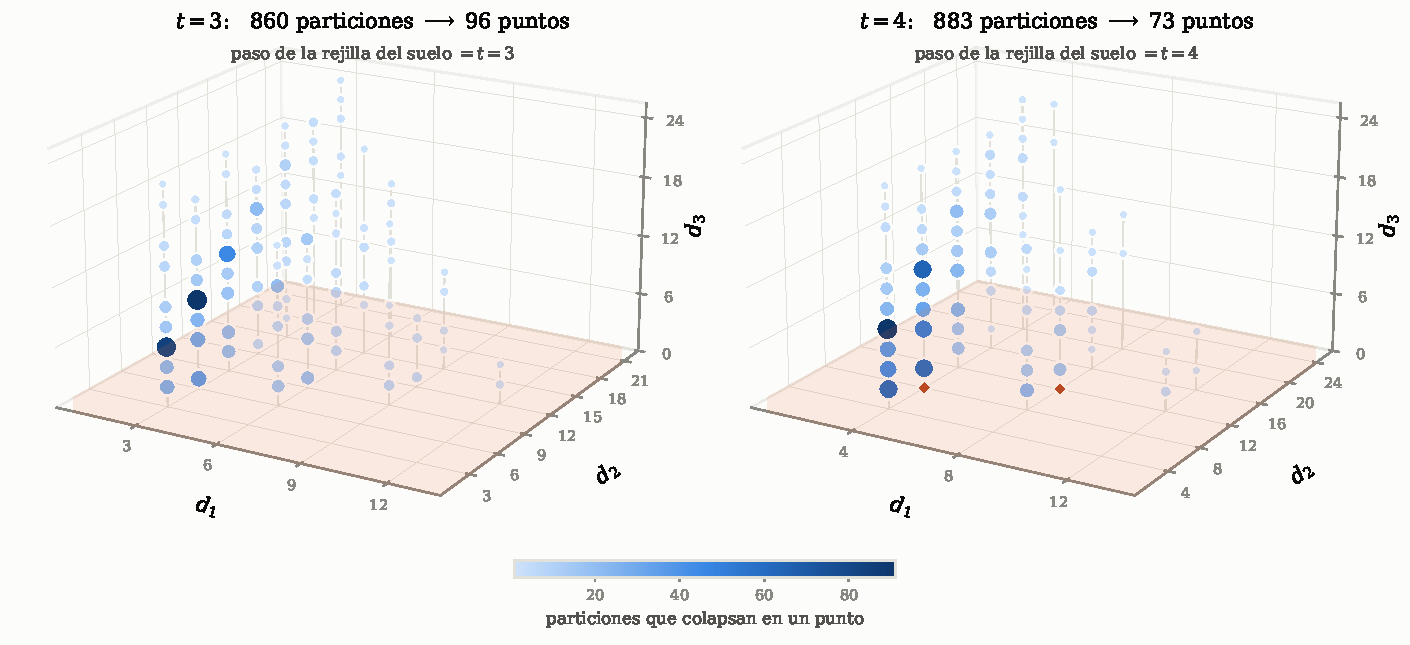
\includegraphics[width=\textwidth]{fig_image_es.pdf}
\caption{La imagen de $\lambda\mapsto(d_1,d_2,d_3)$ sobre todas las $\lambda$ con $|\lambda|\le20$ y
a lo sumo $t+2$ filas, para $t=3$ (izquierda) y $t=4$ (derecha), tomada \emph{salvo el intercambio de
$d_1$ y $d_2$}, bajo el cual \eqref{eq:main} es simétrica; sin esa identificación, y con $A$ y $B$ en
el orden $r_A\le r_B$ del Teorema \ref{thm:main}, los dos paneles llevan $126$ y $92$ puntos en vez
de $96$ y $73$. La compresión es el asunto de la figura: $860$
particiones aterrizan sobre $96$ ternas a la izquierda y $883$ sobre $73$ a la derecha, y el color y
el área dan el número de particiones que va a parar a cada una. El paso de la rejilla del suelo es $t$, pues
$d_1,d_2\in t\ZZ$ por la Proposición \ref{prop:quotient}; el plano sombreado $d_3=0$ es el lugar
concéntrico del Corolario \ref{cor:zero}, donde $s_\lambda$ se anula, así que esas formas no están
en la imagen y se dibujan sobre el plano como rombos. Los dos paneles son las dos paridades, que es
el contenido de la Proposición \ref{rem:lattice}: el impar no lleva ningún rombo, y no puede
llevarlo; el par lleva dos, que son entre ambos la imagen de $32$ particiones.}
\label{fig:image}
\end{figure}

La Figura \ref{fig:image} es una mitad de la imagen: muestra qué ternas se dan, no qué esconde una
terna. La Figura \ref{fig:fibres} es la otra mitad. Sobre cada celda del suelo $(d_1,d_2)$ se levanta
la columna de los tamaños $|\lambda|$ que aterrizan ahí, de modo que una columna es un conjunto de
particiones de tamaños distintos sobre las que $\Phi_t$ toma un único y mismo valor ---y las columnas
no se adelgazan al crecer $|\lambda|$, porque los valores están confinados a un retículo y las
particiones no. La más visible es la fibra de la partición vacía: en $t=3$ el invariante
$I_3=(3,3,2,+1)$ lo comparten $26$ particiones, de $19$ tamaños distintos entre $0$ y $20$, así que
$\Phi_3$ no distingue $\varnothing$ de una forma de veinte cajas.

\begin{figure}[!ht]
\centering
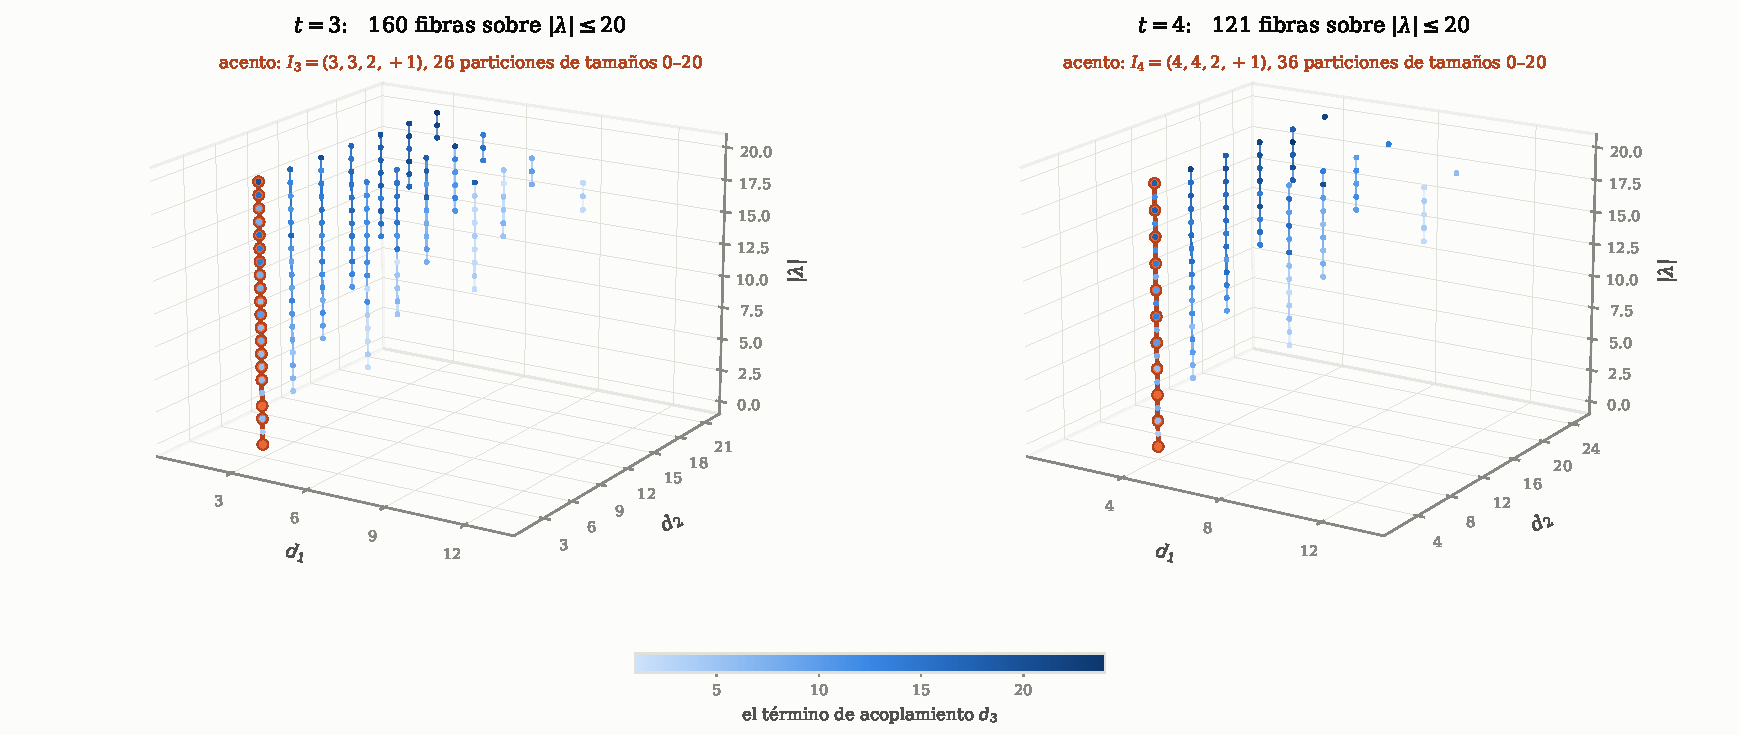
\includegraphics[width=\textwidth]{fig_fibres_es.pdf}
\caption{Las fibras del invariante de la evaluación \eqref{eq:invariant}, complemento de la Figura
\ref{fig:image}: el mismo rango $|\lambda|\le20$, con el término de acoplamiento pasado al color y el
tamaño $|\lambda|$ en el eje vertical. Una columna es una fibra, así que su altura es el rango de
tamaños que este alfabeto no sabe separar; las marcas del suelo son el retículo $t\ZZ$ de la
Proposición \ref{prop:quotient}, y solo está ocupada la mitad $d_1\le d_2$ porque la terna se toma
salvo el intercambio, como en la Figura \ref{fig:image}. Que todas las marcas de una columna lleven
el mismo valor está computado, no supuesto: sobre las $860$ particiones de la izquierda y las $883$
de la derecha el bialternante es constante en cada fibra hasta $10^{-37}$. La columna en color de
acento es la fibra de $\lambda=\varnothing$.}
\label{fig:fibres}
\end{figure}

La Figura 
\ref{fig:fibres} precisa una cosa sobre \eqref{eq:invariant}: $I_t$ es completo pero no mínimo.
El numerador de \eqref{eq:main} es simétrico en $d_1,d_2,d_3$, de modo que el valor solo ve el multiconjunto
$\{d_1,d_2,d_3\}$ junto con el signo, y esa es una reducción real ---sobre $t=4$ y $|\lambda|\le20$
los $121$ invariantes toman solo $110$ valores, mientras que en $t=3$ y el mismo rango los dos
recuentos coinciden. Esa reducción es toda la que hay: por debajo del multiconjunto y del signo no se
pierde nada, y es aquí donde la compresión anunciada en la introducción se vuelve un enunciado exacto
en vez de una cota superior.

\begin{proposition}[el multiconjunto y el signo son exactamente lo que se ve]\label{prop:minimal}
Fíjese $t\ge2$ y sean $\lambda,\mu\in\PP_N$ con $\Phi_t(\lambda;z)\not\equiv0$. Entonces
\[
\Phi_t(\lambda;z)=\Phi_t(\mu;z)
\quad\Longleftrightarrow\quad
\{d_1,d_2,d_3\}(\lambda)=\{d_1,d_2,d_3\}(\mu)\ \text{como multiconjuntos y}\
\varepsilon_\lambda=\varepsilon_\mu .
\]
\end{proposition}

\begin{proof}
$(\Leftarrow)$ es \eqref{eq:main}, cuyo miembro derecho es simétrico en los tres argumentos. Para
$(\Rightarrow)$, obsérvese primero que $\Phi_t(\mu;z)=\Phi_t(\lambda;z)\not\equiv0$, luego $\mu$
tiene también perfil no degenerado y $\tilde d_3(\mu)\ne0$, y los dos invariantes están definidos.
Escribamos $d=d(\lambda)$ y $e=d(\mu)$, con las seis entradas $\ge1$, y pongamos $u=z^{1/2}$, de modo
que $2\sinh(v\theta/2)=u^{v}-u^{-v}$ con exponentes enteros. El denominador de \eqref{eq:main}
depende sólo de $t$, así que la hipótesis es
\[
\varepsilon_\lambda\prod_{i=1}^{3}\bigl(u^{d_i}-u^{-d_i}\bigr)
=\varepsilon_\mu\prod_{i=1}^{3}\bigl(u^{e_i}-u^{-e_i}\bigr).
\]
Usando $u^{v}-u^{-v}=u^{-v}(u^{2v}-1)$ en cada factor y poniendo $D=\sum_id_i$, $E=\sum_ie_i$,
\[
\varepsilon_\lambda\,u^{-D}\prod_{i}\bigl(u^{2d_i}-1\bigr)
=\varepsilon_\mu\,u^{-E}\prod_{i}\bigl(u^{2e_i}-1\bigr).
\]
Cada producto es un polinomio de término constante $(-1)^3=-1$, así que el exponente más bajo que
aparece es $-D$ a la izquierda y $-E$ a la derecha, con coeficientes $-\varepsilon_\lambda$ y
$-\varepsilon_\mu$: luego $D=E$ y $\varepsilon_\lambda=\varepsilon_\mu$, y los dos productos
coinciden. Ahora bien, $u^{2v}-1=\prod_{m\mid2v}Q_m(u)$, donde $Q_m$ es el $m$-ésimo polinomio
ciclotómico --- escrito $Q$ y no $\Phi$, que en este artículo es el objeto. Los $Q_m$ son
irreducibles y distintos dos a dos, así que por factorización única en $\ZZ[u]$ los dos miembros
llevan el mismo multiconjunto de factores ciclotómicos,
\[
\biguplus_i\{m:m\mid 2d_i\}=\biguplus_i\{m:m\mid 2e_i\} .
\]
Su mayor elemento es $\max_i2d_i$ a la izquierda y $\max_i2e_i$ a la derecha, luego coinciden;
borrando de cada lado una copia del conjunto de divisores de ese máximo, y repitiendo dos veces más,
sale $\{2d_1,2d_2,2d_3\}=\{2e_1,2e_2,2e_3\}$.
\end{proof}

\noindent El par (multiconjunto, signo) es entonces un invariante \emph{completo y separador} para
esta evaluación fuera del lugar de anulación --- completo porque el valor factoriza a través de él,
separador porque datos distintos dan valores distintos ---, y eso es un teorema y no un rango. Nos
quedamos a las puertas de llamarlo \emph{mínimo} sin más, porque la minimalidad es relativa a una
clase de invariantes que habría que fijar antes. La hipótesis $\Phi_t(\lambda;z)\not\equiv0$ no es
eliminable y no es un defecto: sobre el lugar de anulación todo invariante colapsa a un único valor,
que es la razón de que \eqref{eq:invariant} mande todo ese lugar a $0$. Mantenemos allí la forma
ordenada porque $d_3$ es la coordenada que aporta el par recíproco y las otras dos no, y el Corolario
\ref{cor:fibregf} describe las fibras de cualquiera de los dos, ya que difieren por una simetría del
numerador y no por nada que el retículo vea.

\begin{proposition}[una forma más corta del signo]\label{rem:sign}
Sea el perfil de residuos no degenerado y $\tilde d_3\ne0$, y ordénense las dos clases
distinguidas de modo que $r_A\le r_B$. Entonces
\begin{equation}\label{eq:shortsign}
\boxed{\;\;\varepsilon_\lambda\;=\;(-1)^{\lfloor t/2\rfloor}\,\sgn(\sigma)\,(-1)^{\,r_A+r_B}\,
\sgn(\tilde d_3)\;\;}
\end{equation}
donde $\sigma$ es la permutación de la \S\ref{sec:background}.
\end{proposition}

\begin{proof}
Sea $w$ la palabra de residuos de $\beta(\lambda)$ leída en orden creciente de columna. Como $\beta$
decrece con el índice de columna, agrupar las partes por clase con los valores decreciendo dentro de
cada clase es la ordenación estable de $w$, luego $\sgn(\sigma)=(-1)^{\inv(w)}$. Ambos miembros de
\eqref{eq:shortsign} llevan el factor $\sgn(\tilde d_3)$, y $\sgn(a_1-b_1)=(-1)^{[a_1<b_1]}$,
de modo que por \eqref{eq:sign} la afirmación equivale a
\begin{equation}\label{eq:signparity}
j_{A_1}+j_{B_1}+\inv(w)+\inv(b_S)+[a_1<b_1]\;\equiv\;
\Bigl\lfloor\tfrac t2\Bigr\rfloor+t+\binom{N+1}{2}+r_A+r_B \pmod 2 .
\end{equation}

Usamos un único conteo de paridad. Sea $u$ una palabra, $p$ una posición, $c=u_p$, y sea $I(p)$ el
número de inversiones de $u$ en las que participa $p$; escribamos $\nu_{<c}$ para el número de letras
de $u$ estrictamente menores que $c$ y $e_p$ para el número de apariciones de $c$ estrictamente antes
de $p$. Poniendo $x=\#\{j<p:u_j>c\}$, las posiciones anteriores a $p$ se reparten como
$p-1=x+e_p+\#\{j<p:u_j<c\}$ y las letras menores que $c$ como
$\nu_{<c}=\#\{j<p:u_j<c\}+\#\{j>p:u_j<c\}$, de donde
\begin{equation}\label{eq:parity}
I(p)\;=\;x+\#\{j>p:u_j<c\}\;=\;2x+e_p+\nu_{<c}-(p-1)\;\equiv\;(p-1)+\nu_{<c}+e_p \pmod 2 .
\end{equation}
Como $b_S$ es $w$ con las letras de las posiciones $j_{A_1}$ y $j_{B_1}$ borradas,
\[
\inv(w)-\inv(b_S)=I(j_{A_1})+I(j_{B_1})
-\bigl[\,\{j_{A_1},j_{B_1}\}\ \text{es una inversión de }w\,\bigr],
\]
y $\inv(w)+\inv(b_S)\equiv\inv(w)-\inv(b_S)$, así que \eqref{eq:parity} calcula el miembro izquierdo
de \eqref{eq:signparity}.

En el perfil de dos clases $r_A<r_B$, y $w$ lleva $r_A$ dos veces, $r_B$ dos veces y cada uno de los
demás residuos una vez. Como $\beta$ decrece con el índice de columna, $a_1>a_2$ sitúa $j_{A_1}$ en
la \emph{primera} aparición de $r_A$, luego allí $e=0$, y lo mismo en $j_{B_1}$. Las letras menores
que $r_A$ son una copia de cada uno de $0,\dots,r_A-1$, luego $\nu_{<r_A}=r_A$; las menores que $r_B$
son esas mismas junto con la segunda copia de $r_A$, luego $\nu_{<r_B}=r_B+1$. Las dos posiciones
forman una inversión exactamente cuando la letra mayor va primero, es decir cuando
$j_{B_1}<j_{A_1}$, es decir cuando $a_1<b_1$. Por tanto
\begin{multline*}
\inv(w)-\inv(b_S)\;\equiv\;(j_{A_1}-1+r_A)+(j_{B_1}-1+r_B+1)+[a_1<b_1]\\
\equiv\;j_{A_1}+j_{B_1}+r_A+r_B+1+[a_1<b_1],
\end{multline*}
y al sustituir esto en \eqref{eq:signparity} las columnas y $[a_1<b_1]$ se cancelan por pares y queda
$\lfloor t/2\rfloor+t+\binom{N+1}{2}\equiv1$.

En el perfil de tamaño tres $r_A=r_B=:r$ y la clase $\{p>q>p'\}$ ocupa las columnas $j_1<j_2<j_3$ con
$A=\{p,q\}$ y $B=\{q,p'\}$, de modo que $j_{A_1}=j_1$ y $j_{B_1}=j_2$ llevan la misma letra $r$, con
$e=0$ y $e=1$ respectivamente y $\nu_{<r}=r$ en ambos; dos letras iguales no forman inversión, y
$a_1>b_1$. Luego $\inv(w)-\inv(b_S)\equiv j_1+j_2+1$, que es de nuevo la expresión anterior porque
$r_A+r_B=2r$ y $[a_1<b_1]=0$, y \eqref{eq:signparity} se reduce a la misma congruencia.

Por último $N=t+2$, así que esa congruencia dice
$\lfloor t/2\rfloor+t+\binom{t+3}{2}\equiv1$: para $t=2m$ sus tres términos son $m$, $0$ y $m+1$, y
para $t=2m+1$ son $m$, $1$ y $m$. Ambas sumas son impares, y la identidad vale para todo $t\ge2$.
\end{proof}

La ordenación por residuo no es una comodidad, y vale la pena decir por qué. Intercambiar los dos
bloques cambia el signo de $\kappa_{11}$, el del Lema \ref{lem:L4} --- por su factor
$\sgn(a_1-b_1)$ --- y también el de
$\sgn(\tilde d_3)$, luego deja invariante a $\varepsilon_\lambda$, que es su producto; como no
puede ser de otro modo, porque $\varepsilon_\lambda$ va unido a $\lambda$. El miembro derecho de
arriba \emph{no} queda invariante: $(-1)^{r_A+r_B}$ es simétrico, así que solo cambia de signo su
último factor. Sin una regla que fije cuál de los bloques es $A$, el miembro derecho no es siquiera
una función de $\lambda$. La hipótesis entra en la demostración en un único punto: es lo que hace
que $\nu_{<r_A}=r_A$ y $\nu_{<r_B}=r_B+1$ y no al revés, y suprimirla intercambia esos dos conteos y
rompe \eqref{eq:signparity}.

Leída al revés, \eqref{eq:shortsign} dice que $\Phi_t$ es función de un dato combinatorio pequeño y
de nada más, y lo dice para todo $t$ y no sobre un rango: por el Teorema \ref{thm:main} el triple
$(d_1,d_2,d_3)$ determina $\Phi_t$ salvo signo, y añadiendo $\sgn(\sigma)$, el par ordenado
$r_A\le r_B$ y la \emph{orientación} $\sgn(\tilde d_3)$ lo determina por completo. La
forma de $\lambda$ no entra en ninguna otra parte. La orientación no es opcional, y esa parte sigue
siendo una comprobación y no una demostración: sobre $t\le6$ y $|\lambda|\le14$, poner
$\sgn(a_1-b_1)$ en su lugar deja colisiones en $t=2$.

%======================================================================
\section{Demostración del Teorema \ref{thm:main}}\label{sec:proof}

La demostración usa el determinante de Vandermonde, el desarrollo de Laplace y un lema de
cancelación. Damos los pasos por separado para que quien contraste los guiones auxiliares pueda
localizar cualquier discrepancia.

\begin{figure}[!ht]
\centering
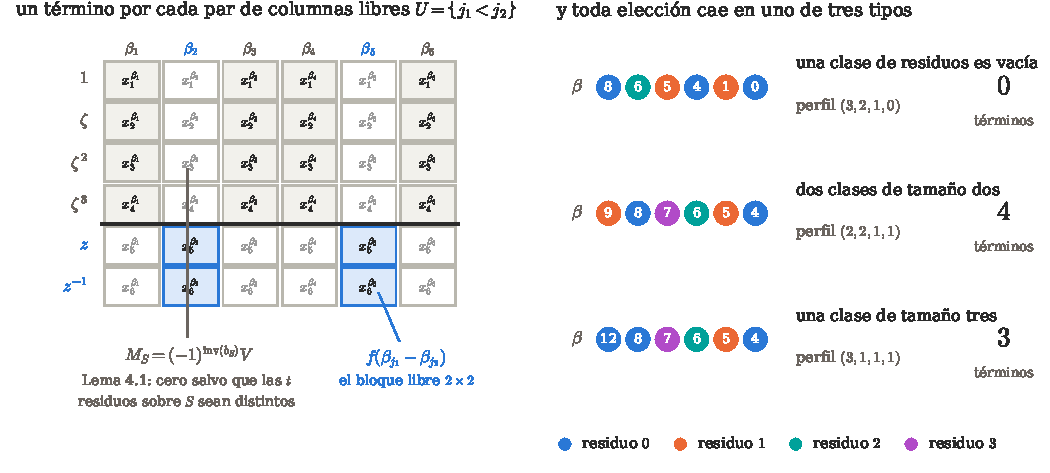
\includegraphics[width=\textwidth]{fig_laplace_es.pdf}
\caption{La arquitectura de la demostración, dibujada con $t=4$, $N=6$. \emph{Izquierda:} el
determinante $\det(x_i^{\beta_j})$ desarrollado por las $t$ filas congeladas. Cada elección de las
dos columnas $U=\{j_1<j_2\}$ que se dejan a las filas libres $z,z^{-1}$ deja un menor $t\times t$
$M_S$ sobre las columnas complementarias, que por el Lema \ref{lem:L1} vale $\pm V$ o cero, por el
bloque $2\times2$ $f(\beta_{j_1}-\beta_{j_2})$. \emph{Derecha:} por el recuento del exceso dos
\eqref{eq:excess} sólo hay tres perfiles de residuos, uno por fila, cada uno sobre un beta-conjunto
que lo realiza; el número de la derecha es cuántas elecciones de $U$ sobreviven, contado y no
afirmado --- $0$, $4$ y $3$, que es la tricotomía sobre la que se organiza la sección. El color es
la clase de residuos. Calculada por \texttt{anc/fig\_proof.py}.}
\label{fig:laplace}
\end{figure}

El desarrollo en sí es el movimiento habitual de esta literatura y no reclamamos nada por él: Albion
\cite{Alb25} aplica el desarrollo de Laplace a un determinante de esta forma \emph{según la
estructura de bloques dada}, manteniendo fijo un primer conjunto de filas, siguiendo a Krattenthaler
y a Ciucu--Krattenthaler. Lo particular aquí no es el desarrollo, sino con qué se topa.

Lo que el argumento hace en realidad es clasificar, no calcular. Desarrollar por las $t$ filas
congeladas deja un término por cada manera de elegir qué dos columnas \emph{no} lo están, y el
recuento del exceso dos dice que toda elección cae en exactamente uno de tres tipos combinatorios:
no sobrevive ninguna (una clase de residuos es vacía), sobreviven cuatro (dos clases de tamaño dos) o
sobreviven tres (una clase de tamaño tres). Todo lo que sigue es contabilidad dentro de un tipo, y el
Lema \ref{lem:L5} muestra que los dos últimos son un mismo enunciado visto dos veces. La Figura \ref{fig:laplace} es esa frase dibujada.

\begin{lemma}\label{lem:L1}
Sea $S$ un conjunto de $t$ columnas y $M_S=\det(\zeta^{k\beta_j})_{0\le k<t,\,j\in S}$. Entonces
$M_S=0$ salvo que los residuos $\{\beta_j\bmod t:j\in S\}$ sean dos a dos distintos, en cuyo caso
$M_S=(-1)^{\inv(b_S)}V$.
\end{lemma}

\begin{proof}
Como $\zeta^{k\beta_j}=(\zeta^{\beta_j})^k$, la matriz es de Vandermonde en los valores
$y_j=\zeta^{\beta_j}$, cuyo determinante es $\prod_{j<j'}(y_{j'}-y_j)$. El valor $y_j$ depende de
$\beta_j$ solo módulo $t$, luego dos columnas de $S$ que compartan residuo anulan el determinante. Si
los residuos son dos a dos distintos, $|S|=t$ obliga a $\{y_j\}_{j\in S}=\zt$ como conjunto, y el
determinante de Vandermonde es alternante en sus argumentos, luego vale $V$ por el signo de la
permutación que ordena $b_S$ crecientemente, que es $(-1)^{\inv(b_S)}$.
\end{proof}

\begin{lemma}\label{lem:L2}
$\det\bigl(x_i^{N-j}\bigr)_{i,j=1}^{N}=(-1)^{\binom t2}\,V\,(z^t-1)(z^{-t}-1)(z-z^{-1})$ para el
alfabeto $x=(1,\zeta,\dots,\zeta^{t-1},z,z^{-1})$ en ese orden.
\end{lemma}

\begin{proof}
El determinante es $\prod_{i<i'}(x_i-x_{i'})$. Los pares dentro de $\zt$ aportan
$\prod_{k<k'}(\zeta^k-\zeta^{k'})=(-1)^{\binom t2}V$; los pares $(\zeta^k,z)$ aportan
$\prod_k(\zeta^k-z)=(-1)^t(z^t-1)$ y los pares $(\zeta^k,z^{-1})$ aportan $(-1)^t(z^{-t}-1)$; el
último par aporta $z-z^{-1}$. Los dos factores $(-1)^t$ se cancelan.
\end{proof}

\noindent Lo calculamos porque son tres líneas, no porque sea desconocido: un determinante sobre un
alfabeto cerrado bajo $x\mapsto x^{-1}$, evaluado en forma de producto cerrado, es exactamente el
asunto del complemento de Krattenthaler al cálculo de determinantes \cite[\S5.11]{KratADCC}, cuyo
Lema 20 lleva entre sus casos particulares las fórmulas del denominador de Weyl para $B_n$, $C_n$ y
$D_n$. Lo que esa literatura no evalúa ---y lo que el lema siguiente necesita--- es ese mismo
determinante con una órbita de raíces de la unidad dentro del alfabeto.

\begin{lemma}\label{lem:L3}
Sea $\mathcal U$ el conjunto de pares $U=\{j_1<j_2\}$ de columnas cuyo complementario $S_U$ lleva las
$t$ clases de residuos. Entonces
\[
\Phi_t(\lambda;z)=\frac{(-1)^{\,t+\binom{N+1}{2}}}{(z^t-1)(z^{-t}-1)(z-z^{-1})}
\sum_{U\in\mathcal U}(-1)^{\,j_1+j_2+\inv(b_{S_U})}\,f(\beta_{j_1}-\beta_{j_2}).
\]
\end{lemma}

\begin{proof}
Desarrollando el numerador por Laplace a lo largo de las primeras $t$ filas,
\[
\det\bigl(x_i^{\beta_j}\bigr)=\sum_{|S|=t}(-1)^{\binom{t+1}{2}+\sum_{j\in S}j}\,M_S\,C_{S^c},
\]
donde para $S^c=\{j_1<j_2\}$ el menor complementario $2\times2$ es
$z^{\beta_{j_1}-\beta_{j_2}}-z^{-(\beta_{j_1}-\beta_{j_2})}=f(\beta_{j_1}-\beta_{j_2})$. Por el Lema
\ref{lem:L1} solo contribuyen los $S$ con residuos dos a dos distintos. Escribiendo
$\sum_{j\in S}j=\binom{N+1}{2}-j_1-j_2$ y dividiendo por el Lema \ref{lem:L2}, los factores $V$ se
cancelan y $(-1)^{\binom{t+1}{2}-\binom{t}{2}}=(-1)^t$.
\end{proof}

Si algún $n_i=0$, ningún $S$ de tamaño $t$ lleva todos los residuos, $\mathcal U=\varnothing$ y
$\Phi_t=0$: es el Teorema \ref{thm:main}(i). En caso contrario todos los $n_i\ge1$ y por
\eqref{eq:excess} o bien dos clases tienen tamaño dos, y entonces $S_U$ debe descartar un elemento de
cada una y $|\mathcal U|=4$, o bien una clase tiene tamaño tres, y entonces $S_U$ descarta dos de los
tres y $|\mathcal U|=3$.

\begin{lemma}[el movimiento de columna]\label{lem:L4}
Sean $A$ y $B$ clases distintas de tamaño dos, en las columnas $j_{A_1}<j_{A_2}$ y
$j_{B_1}<j_{B_2}$. Para $i,j\in\{1,2\}$ sea $U_{ij}$ el par formado por la columna de $a_i$ y la de
$b_j$, y sea $\kappa_{ij}=(-1)^{\,j_{A_i}+j_{B_j}+\inv(b_{S_{U_{ij}}})}\sgn(a_i-b_j)$, de modo que
el término $U_{ij}$ del Lema \ref{lem:L3} vale $\kappa_{ij}f(a_i-b_j)$. Entonces
$\kappa_{ij}=\kappa_{11}(-1)^{i-1}(-1)^{j-1}$.
\end{lemma}

\begin{proof}
Fijemos $j$ y comparemos $i=1$ con $i=2$. Los conjuntos $S_{U_{1j}}$ y $S_{U_{2j}}$ difieren solo en
que el primero contiene la columna $j_{A_2}$ y el segundo la columna $j_{A_1}$, y la letra que llevan
es el residuo $r_A$ en ambos casos. Pasar de una palabra a la otra mueve esa letra a través de
exactamente las columnas conservadas estrictamente entre $j_{A_1}$ y $j_{A_2}$, y ninguna de esas
letras es igual a $r_A$ porque la clase $A$ tiene solo dos elementos; cada cruce cambia la paridad de
$\inv$. Por tanto
\[
(-1)^{\inv(b_{S_{U_{1j}}})-\inv(b_{S_{U_{2j}}})}
=(-1)^{(j_{A_2}-j_{A_1}-1)-[\,a_2<b_j<a_1\,]},
\]
usando que $\beta$ es estrictamente decreciente en el índice de columna, de modo que $j_{B_j}$ está
estrictamente entre $j_{A_1}$ y $j_{A_2}$ exactamente cuando $a_2<b_j<a_1$. Multiplicando por el
factor de Laplace $(-1)^{j_{A_1}+j_{A_2}}$,
\[
\frac{\kappa_{1j}}{\kappa_{2j}}
=(-1)^{2j_{A_2}-1}(-1)^{[\,a_2<b_j<a_1\,]}\sgn(a_1-b_j)\sgn(a_2-b_j)=-1,
\]
porque $\sgn(a_1-b_j)\sgn(a_2-b_j)=-1$ exactamente cuando $b_j$ está entre $a_2$ y $a_1$.
Intercambiando los papeles de $A$ y $B$ se obtiene $\kappa_{i1}/\kappa_{i2}=-1$.
\end{proof}

\begin{lemma}\label{lem:L5}
Para todos $c,p,q$ y todos $u,v$,
\begin{align*}
\text{\rm(a)}&\quad \sum_{\epsilon,\eta\in\{\pm1\}}\epsilon\eta\,f(c+\epsilon p+\eta q)=f(c)f(p)f(q),\\
\text{\rm(b)}&\quad f(2u)-f(2u+2v)+f(2v)=-f(u)f(v)f(u+v).
\end{align*}
\end{lemma}

\begin{proof}
Para (a), $\sum_{\epsilon,\eta}\epsilon\eta\,z^{c+\epsilon p+\eta q}
=z^{c}\bigl(\sum_\epsilon\epsilon z^{\epsilon p}\bigr)\bigl(\sum_\eta\eta z^{\eta q}\bigr)
=z^{c}f(p)f(q)$, y el mismo cálculo para los exponentes negativos da $z^{-c}(-f(p))(-f(q))$;
réstese. Para (b), pónganse $s=z^u$, $w=z^v$ y desarróllese
$(s-s^{-1})(w-w^{-1})(sw-s^{-1}w^{-1})$: los ocho términos se recombinan como
$(s^2w^2-s^{-2}w^{-2})-(s^2-s^{-2})-(w^2-w^{-2})=f(2u+2v)-f(2u)-f(2v)$.
\end{proof}

\begin{proof}[Demostración del Teorema \ref{thm:main}]
En el perfil de dos clases, los Lemas \ref{lem:L3} y \ref{lem:L4} dan
\[
\sum_{U\in\mathcal U}(\cdots)=\kappa_{11}\sum_{i,j}(-1)^{i-1}(-1)^{j-1}f(a_i-b_j).
\]
Escribiendo $a_i=\alpha+\epsilon_ip$ y $b_j=\gamma+\eta_jq$ con $p=d_1/2$, $q=d_2/2$ y
$\epsilon=\eta=(+1,-1)$, se tiene $a_i-b_j=c+\epsilon_ip-\eta_jq$ con $c=\alpha-\gamma$. Sustituyendo
$\eta$ por $-\eta$, la suma se convierte en
$-\sum_{\epsilon,\eta}\epsilon\eta f(c+\epsilon p+\eta q)$, que vale $-f(c)f(p)f(q)$ por el Lema
\ref{lem:L5}(a). Como $(z^t-1)(z^{-t}-1)=2-z^t-z^{-t}=-f(t/2)^2$ y $z-z^{-1}=f(1)$, los dos signos
menos se cancelan, y sustituyendo $f(u)=2\sinh(u\theta)$ los factores numéricos se cancelan. Aquí
$2c=\tilde d_3$. Si $\tilde d_3=0$, entonces $f(c)=0$ y la suma entera se anula, que es la primera
afirmación de {\rm(ii)}; en caso contrario
$\sinh(c\theta)=\sgn(\tilde d_3)\sinh(d_3\theta/2)$, lo que da \eqref{eq:main} con
$\varepsilon_\lambda=(-1)^{\,t+\binom{N+1}{2}}\kappa_{11}\sgn(\tilde d_3)$, que es
\eqref{eq:sign} por la definición de $\kappa_{11}$ en el Lema \ref{lem:L4}.

Para el perfil de tamaño tres $\{p>q>r\}$ en las columnas $j_1<j_2<j_3$ se aplica el mismo argumento
de movimiento de columna, de nuevo porque ninguna letra estrictamente entre dos de esas columnas
lleva el residuo de la clase, y da signos alternantes $(\varsigma,-\varsigma,\varsigma)$ para los
tres términos $f(p-q)$, $f(p-r)$, $f(q-r)$. Por el Lema \ref{lem:L5}(b) con $u=(p-q)/2$,
$v=(q-r)/2$ la suma es $-\varsigma f(u)f(v)f(u+v)$, que es la fórmula de dos clases para $A=\{p,q\}$,
$B=\{q,r\}$ con $\varsigma=\kappa_{11}$. Equivalentemente, la cuarta selección ausente del perfil de
dos clases descartaría $q$ dos veces y su término lleva $f(0)=0$, de modo que los dos perfiles son un
solo enunciado.
\end{proof}

Todos los enunciados de este artículo se comprobaron además numéricamente; los recuentos se recogen
una sola vez, en la \S\ref{sec:verif}, en lugar de repetirse según van surgiendo.

%======================================================================
\section{Independencia en el lugar recíproco}\label{sec:independence}

El Teorema 5.3 de \cite{AK25} está enunciado para variables libres, y $(z,\zb)$ no es un par libre.
Nada de esta sección lo contradice: el lugar recíproco queda fuera de sus hipótesis, no en contra de
ellas, y lo que hacemos aquí es determinar en qué se convierte allí su criterio. Leída al pie de la
letra, \eqref{eq:AK53} diría que para $\ell(\lambda)\le2$ se tiene
$s_\lambda(z,\zb,\zt)=s_\lambda(z,\zb)$ exactamente sobre los $t$-núcleos. El Teorema
\ref{thm:main} evalúa el miembro izquierdo para toda $\lambda$, y al comparar ambos se ve que el
lugar recíproco lleva más soluciones: exactamente una familia. Medir cuánto sobrevive un criterio a
una degeneración es una manera de decir lo afilado que era, y la respuesta aquí es que lo es salvo
una sola familia.

Aislamos primero cuándo $\Phi_t$ degenera en un solo carácter.

\begin{lemma}\label{lem:single}
$\Phi_t(\lambda;z)=\pm\chi_k(z)$ para algún $k\ge0$ si y solo si el multiconjunto $\{d_1,d_2,d_3\}$
contiene $t$ al menos dos veces, y en tal caso la entrada restante vale $2(k+1)$.
\end{lemma}

\begin{proof}
Pongamos $u=z^{1/2}$, de modo que $2\sinh(d_i\theta/2)=u^{d_i}-u^{-d_i}$,
$2\sinh(t\theta/2)=u^{t}-u^{-t}$ y $2\sinh\theta=u^{2}-u^{-2}$; todos los exponentes son enteros. Por
\eqref{eq:main}, la igualdad afirmada es
\[
\prod_{i=1}^{3}\bigl(u^{d_i}-u^{-d_i}\bigr)
=\pm\bigl(u^{t}-u^{-t}\bigr)^{2}\bigl(u^{2k+2}-u^{-2k-2}\bigr).
\]
Usando $u^{n}-u^{-n}=u^{-n}(u^{2n}-1)$ en cada factor y comparando los prefactores monomiales se
obtiene $d_1+d_2+d_3=2t+2(k+1)$ junto con
\[
\prod_{i=1}^{3}\bigl(u^{2d_i}-1\bigr)=\pm\bigl(u^{2t}-1\bigr)^{2}\bigl(u^{4(k+1)}-1\bigr),
\]
y evaluando en $u=0$ el signo queda fijado en $+$. Ahora $u^{2n}-1=\prod_{m\mid 2n}Q_m(u)$ con
$Q_m$ los polinomios ciclotómicos como en la Proposición \ref{prop:minimal}, que son irreducibles y
distintos dos a dos, de modo que por
factorización única en $\ZZ[u]$ ambos miembros tienen el mismo multiconjunto de factores
ciclotómicos. A la izquierda ese multiconjunto es $\biguplus_i\{m:m\mid 2d_i\}$ y a la derecha
$2\times\{m:m\mid 2t\}\uplus\{m:m\mid 4(k+1)\}$. Su mayor elemento es $\max_i 2d_i$ a la izquierda y
$\max(2t,4(k+1))$ a la derecha; borrando de ambos lados el conjunto de divisores de ese máximo y
repitiendo dos veces más se llega a
\[
\{2d_1,2d_2,2d_3\}=\{2t,\,2t,\,4(k+1)\}
\]
como multiconjuntos, que es lo afirmado. El recíproco es el mismo cálculo leído al revés.
\end{proof}

\begin{theorem}\label{thm:extra}
Sea $\ell(\lambda)\le2$. Entonces
\[
\Phi_t(\lambda;z)=s_\lambda(z,\zb)
\]
---una igualdad, y no una igualdad salvo signo--- si y solo si o bien
$\lambda=\core_t(\lambda)$, o bien
\begin{equation}\label{eq:extra}
t\ \text{es par}\quad\text{y}\quad \lambda=\Bigl(\lambda_2+\tfrac{3t}{2}-1,\ \lambda_2\Bigr)
\quad\text{con}\quad \tfrac t2\le\lambda_2\le t-1 .
\end{equation}
En el segundo caso $\{d_1,d_2,d_3\}=\{3t,t,t\}$ y $\varepsilon_\lambda=+1$, mientras que
$\core_t(\lambda)=\bigl(\tfrac t2-1+j,j\bigr)$ y $\quot_t(\lambda)$ tiene como única componente no
vacía $(2)$, en la posición $j=\lambda_2-\tfrac t2$.
\end{theorem}

La Figura \ref{fig:locus} es el enunciado computado en vez de afirmado: ambas familias están
dibujadas sobre un rango de $t$, y el $t$ impar donde \eqref{eq:extra} no puede darse es el control.

\begin{figure}[!ht]
\centering
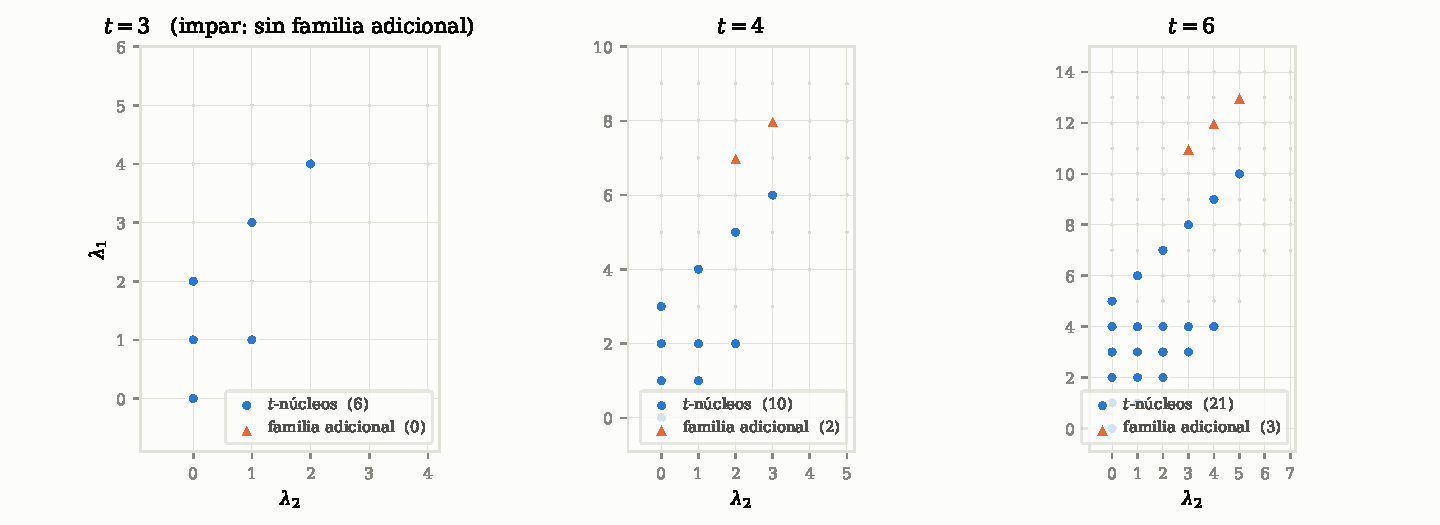
\includegraphics[width=\textwidth]{fig_locus_es.pdf}
\caption{El Teorema \ref{thm:extra}, calculado y no afirmado. Para toda $\lambda$ de dos filas en
rango se evaluaron ambos miembros de $\Phi_t(\lambda;z)=\pm s_\lambda(z,\zb)$; se representan las
particiones donde coinciden, coloreadas por familia. Los círculos son los $t$-núcleos, las soluciones
ya descritas por \eqref{eq:AK53}; los triángulos son la familia adicional \eqref{eq:extra}, que crea
la especialización recíproca. El caso impar $t=3$ es el control: por el Teorema \ref{thm:extra} allí
no puede existir solución adicional, y no se halla ninguna.}
\label{fig:locus}
\end{figure}

\begin{proof}
Como $\ell(\lambda)\le 2$ y $N=t+2$, el conjunto beta es
$\beta(\lambda)=\bigl(A'+t,\;B'+t,\;t-1,t-2,\dots,1,0\bigr)$ donde
\[
A':=\lambda_1+1,\qquad B':=\lambda_2,\qquad A'>B'\ge0 .
\]
El bloque $\{0,1,\dots,t-1\}$ toca cada clase de residuos exactamente una vez, luego ninguna clase es
vacía y las dos partes grandes deciden el perfil. Escribamos $A'=t\alpha+\rho_A$ y
$B'=t\gamma+\rho_B$ con $0\le\rho_A,\rho_B\le t-1$. Como $s_\lambda(z,\zb)=\chi_{\lambda_1-\lambda_2}(z)$,
el Lema \ref{lem:single} dice que la afirmación se cumple exactamente cuando $\{d_1,d_2,d_3\}$
contiene $t$ dos veces y la tercera entrada es $2(\lambda_1-\lambda_2+1)=2(A'-B')$.

\emph{Caso $\rho_A=\rho_B=:\rho$.} Una clase tiene tamaño tres, a saber $\{A'+t,B'+t,\rho\}$, y por el
Teorema \ref{thm:main} los tres argumentos son $d_1=A'-B'$, $d_2=B'+t-\rho=t(\gamma+1)$,
$d_3=A'+t-\rho=t(\alpha+1)$. Aquí $t\mid A'-B'$, digamos $A'-B'=ts$ con $s\ge1$. El par $d_2=d_3=t$
fuerza $\alpha=\gamma=0$, luego $A'=B'$, excluido. El par $d_1=d_3=t$ fuerza $s=1$ y $\alpha=0$,
luego $A'<t$ y $A'=B'+t\ge t$, excluido. El par $d_1=d_2=t$ fuerza $s=1$ y $\gamma=0$, es decir
$A'=B'+t$ con $B'<t$; entonces $\alpha=1$ y la tercera entrada es $d_3=2t=2(A'-B')$, como se
requiere. Este caso aporta pues exactamente las $\lambda$ con $A'=B'+t$, $B'<t$.

\emph{Caso $\rho_A\ne\rho_B$.} Dos clases tienen tamaño dos, a saber $\{A'+t,\rho_A\}$ y
$\{B'+t,\rho_B\}$, y los tres argumentos son
\[
d_A=t(\alpha+1),\qquad d_B=t(\gamma+1),\qquad
d_3=\bigl|\,t(\alpha-\gamma)+2(\rho_A-\rho_B)\,\bigr| .
\]
Si $d_A=d_B=t$ entonces $\alpha=\gamma=0$, luego $A',B'<t$ y $d_3=2|\rho_A-\rho_B|=2(A'-B')$
automáticamente: toda tal $\lambda$ es solución. En otro caso exactamente uno de $d_A,d_B$ vale $t$ y
$d_3=t$. Si $\alpha=0$ y $\gamma\ge1$, entonces $|-t\gamma+2(\rho_A-\rho_B)|=t$ con
$|\rho_A-\rho_B|\le t-1$ fuerza $\gamma=2$ y $\rho_A-\rho_B=t/2$; pero entonces
$\lambda_1=A'-1=\rho_A-1<t$ mientras que $\lambda_2=B'\ge2t$, en contra de $\lambda_1\ge\lambda_2$.
Si $\gamma=0$ y $\alpha\ge1$, entonces $|t\alpha+2(\rho_A-\rho_B)|=t$ fuerza, para $\alpha=1$,
$\rho_A=\rho_B$ (excluido), y para $\alpha=2$,
\[
\rho_B-\rho_A=\tfrac t2,
\]
lo que exige $t$ par; $\alpha\ge3$ da $|2(\rho_A-\rho_B)|\ge2t$, imposible. Luego $A'=2t+\rho_A$,
$B'=\rho_B=\rho_A+\tfrac t2$, de donde
\[
\lambda_1=2t+\rho_A-1,\qquad \lambda_2=\rho_A+\tfrac t2,\qquad
\lambda_1-\lambda_2=\tfrac{3t}{2}-1,
\]
y $\rho_B\le t-1$ da $0\le\rho_A\le\tfrac t2-1$, es decir $\tfrac t2\le\lambda_2\le t-1$. La entrada
restante es $d_A=t(\alpha+1)=3t=2(\lambda_1-\lambda_2+1)$, como se requiere. Esto es
\eqref{eq:extra}.

Queda identificar las soluciones del primer caso de cada análisis con los $t$-núcleos. Para
$\ell(\lambda)\le2$ el conjunto beta en dos posiciones es $(A',B')$, y $\lambda$ es un $t$-núcleo si
y solo si ningún número beta puede rebajarse en $t$ hasta una posición no negativa desocupada, es
decir si y solo si $B'<t$ y o bien $A'<t$ o bien $A'=B'+t$. Son exactamente las dos familias
halladas. Por último, en el caso \eqref{eq:extra} la clase $\rho_A$ lleva $\{2t+\rho_A+t,\rho_A\}$,
luego su componente del cociente es $(2)$, toda otra componente es vacía, y el núcleo es el
enunciado.

\emph{El signo.} Las dos familias lo consiguen por razones distintas. Sobre los $t$-núcleos la
igualdad es \eqref{eq:AK53} misma, que es una igualdad y no una igualdad salvo signo, así que no hay
nada que probar. Sobre \eqref{eq:extra}, escríbase $t=2m$ y $\lambda_2=m+j$ con $0\le j\le m-1$, de
modo que $\rho_A=j$ y $\rho_B=m+j$ y
\[
\beta(\lambda)=\bigl(6m+j,\;3m+j,\;2m-1,2m-2,\dots,1,0\bigr).
\]
Reduciendo módulo $t=2m$, la palabra de residuos leída en orden creciente de columna es
\[
w=\bigl(j,\;m+j,\;2m-1,2m-2,\dots,1,0\bigr),
\]
puesto que $6m+j\equiv j$ y $3m+j\equiv m+j$, esto último porque $j\le m-1$. Sus inversiones son de
tres clases: la cola decreciente aporta $\binom{2m}{2}$; la primera letra está por encima de
exactamente las $j$ letras de la cola $0,\dots,j-1$; la segunda, por encima de exactamente las $m+j$
letras $0,\dots,m+j-1$; y las dos primeras letras están en orden creciente, así que no aportan
ninguna. Por tanto
\begin{equation}\label{eq:extrainv}
\inv(w)=\binom{2m}{2}+j+(m+j)=2m^{2}+2j\;\equiv\;0\pmod2 ,
\end{equation}
luego $\sgn(\sigma)=(-1)^{\inv(w)}=+1$ por la primera línea de la prueba de la Proposición
\ref{rem:sign}. Las dos clases distinguidas son $r_A=j<r_B=m+j$, que llevan $A=\{6m+j,\,j\}$ y
$B=\{3m+j,\,m+j\}$, de modo que $\tilde d_3=(6m+2j)-(4m+2j)=2m>0$ y $\sgn(\tilde d_3)=+1$. Los dos
factores restantes de \eqref{eq:shortsign} son $(-1)^{\lfloor t/2\rfloor}=(-1)^{m}$ y
$(-1)^{r_A+r_B}=(-1)^{m+2j}=(-1)^{m}$, cuyo producto es $+1$. Así pues $\varepsilon_\lambda=+1$, y
como $d_1=6m=3t$, $d_2=2m=t$ y $d_3=2m=t$, \eqref{eq:main} dice
\[
\Phi_t(\lambda;z)=\frac{\sinh(3t\theta/2)\sinh^{2}(t\theta/2)}{\sinh^{2}(t\theta/2)\sinh\theta}
=\chi_{\frac{3t}{2}-1}(z)=\chi_{\lambda_1-\lambda_2}(z)=s_\lambda(z,\zb),
\]
sin ningún signo que arrastrar.
\end{proof}

\noindent Lo que compra \eqref{eq:extrainv} no es decoración. Enunciado salvo signo, el Teorema
\ref{thm:extra} dice que la especialización crea una familia de formas sobre las que el twist es
invisible \emph{salvo un signo}, que es un enunciado más débil que el que \eqref{eq:AK53} hace sobre
los núcleos; con el signo resuelto, las dos familias son soluciones de la misma ecuación, y ``el
lugar recíproco adquiere exactamente una familia más'' es literalmente cierto.

\begin{remark}\label{rem:why}
El Lema \ref{lem:single} controla el valor sólo salvo signo, y por eso el signo del Teorema
\ref{thm:extra} necesita el párrafo aparte de arriba en lugar de salir de la clasificación.

La familia adicional pertenece a la especialización y no al alfabeto. El paso es el
\cite[Lema 5.2]{AK25}, sobre el que se apoya el \cite[Teorema 5.3]{AK25}: reduce la independencia a
la anulación de $s_{\lambda/\mu}$ en el alfabeto torcido para todo $\mu\subsetneq\lambda$, y la
reducción usa la independencia lineal de los caracteres universales $f_\mu$ en las variables libres. En el lugar recíproco
$s_\mu(z,\zb)=\chi_{\mu_1-\mu_2}(z)$ depende solo de $\mu_1-\mu_2$, luego $s_{(1)}$, $s_{(2,1)}$ y
$s_{(3,2)}$ coinciden allí y esa independencia deja de estar disponible; el Teorema \ref{thm:extra}
mide la diferencia. Un control confirma la lectura: para $\lambda=(3,1)$ y $t=2$ se tiene
$s_\lambda(\zt,z,\zb)=s_\lambda(z,\zb)$, mientras que $s_\lambda(\zt,x,y)\ne s_\lambda(x,y)$ para
$x,y$ libres.
\end{remark}

Así pues, el criterio no sobrevive intacto a la especialización, y lo que adquiere es pequeño y
nombrable: una familia, para formas de dos filas, indexada por un elemento de orden dos del retículo
de residuos y clasificada por su núcleo y su cociente. Las soluciones adicionales pertenecen al lugar
recíproco y no al alfabeto ---existen porque una especialización ha retirado una independencia lineal
que el argumento original usaba, y ese paso que falta es exactamente lo que mide el Teorema
\ref{thm:extra}.

%======================================================================
\section{Una enumeración en la que sobrevive un parámetro}\label{sec:enum}

Desarrollando $s_\lambda$ sobre tablas semiestándar, el Teorema \ref{thm:main} se convierte en una
fórmula de producto para un recuento pesado. Sea $m_k(T)$ el número de entradas iguales a $k$ en $T$.

\begin{corollary}\label{cor:enum}
Desarrollando $s_\lambda$ sobre tablas semiestándar y aplicando el Teorema \ref{thm:main}: para todo
$t\ge2$ y toda $\lambda\in\PP_{t+2}$,
\[
\sum_{T\in\mathrm{SSYT}(\lambda,\,t+2)}
\zeta^{\,\sum_{k=1}^{t}(k-1)m_k(T)}\;z^{\,m_{t+1}(T)-m_{t+2}(T)}
\;=\;\varepsilon_\lambda\,
\frac{\sinh(d_1\theta/2)\sinh(d_2\theta/2)\sinh(d_3\theta/2)}{\sinh^2(t\theta/2)\sinh\theta}.
\]
\end{corollary}

Para $t=2$ el peso es $(-1)^{m_2(T)}$, y si $\lambda=(c^{\,a})$ es rectangular entonces
$\mathrm{SSYT}(\lambda,4)$ está en biyección con las particiones planas en una caja
$a\times(4-a)\times c$, equivalentemente con las teselaciones de rombos de un hexágono. El Corolario
\ref{cor:enum} es entonces una $(-1)$-enumeración de esos objetos \emph{refinada por un parámetro
libre} $z$, que registra la diferencia entre los números de entradas $3$ y $4$. Poniendo $z=1$ se
recupera el recuento con signo puro, que por \eqref{eq:main} vale $\pm d_1d_2d_3/(2t^2)$: para la
$a=2$, $c=2$ vale $4$; para $a=2$, $c=4$ vale $9$; para $a=3$, $c=3$ vale $-6$.

\begin{example}\label{ex:boxes}
Tomando $\lambda=(c^{\,a})$ con $1\le a\le4$ y $t=2$, la forma tiene a lo sumo cuatro filas, las
tablas son las particiones planas en una caja $a\times(4-a)\times c$, y la forma cerrada da los
recuentos con signo de la Figura \ref{fig:signed}. Leyéndola:
\[
\begin{array}{ll}
1\times3\times c: & \bigl\lfloor (c+2)^2/4\bigr\rfloor,\\[2pt]
2\times2\times c: & (c/2+1)^2 \text{ si } c \text{ es par},\qquad 0 \text{ si } c \text{ es impar},\\[2pt]
3\times1\times c: & (-1)^c\bigl\lfloor (c+2)^2/4\bigr\rfloor,\\[2pt]
4\times0\times c: & (-1)^c .
\end{array}
\]
La tercera fila es la traspuesta de la primera, y por eso los módulos coinciden; la cuarta es la caja
degenerada, donde $s_{(c^4)}(x)=(x_1x_2x_3x_4)^c$ y el alfabeto tiene determinante $-1$. No
reivindicamos estos recuentos concretos como nuevos ---las cajas son pequeñas y el signo aquí es la
especialización $x_2=-1$, no el signo de complementación de las $(-1)$-enumeraciones de Kuperberg---
y los registramos solo para mostrar lo que produce el teorema. Lo que sí parece nuevo es que cada uno
de ellos es el valor en $z\mapsto1$ de un refinamiento de un parámetro con la misma fórmula de
producto.
\end{example}

Los cuadrados perfectos del Ejemplo \ref{ex:boxes} no son un accidente de casos pequeños: son lo que
la lectura por intervalos de la \S\ref{sec:intervals} dice que un rectángulo debe producir.

\begin{proposition}\label{prop:rect}
Sean $t=2$ y $\lambda=(c^{\,a})$ con $1\le a\le4$. Entonces uno de $d_1,d_2,d_3$ vale $2$, y:
\begin{enumerate}
\item[\rm(i)] si $a=4$, los tres valen $2$ sea cual sea $c$ y el recuento es $(-1)^c$: es el
rectángulo completo, donde $s_{(c^4)}(x)=(x_1x_2x_3x_4)^{c}$ se reduce a un monomio y del alfabeto no
queda más que su determinante;
\item[\rm(ii)] si $a\le3$ y $c$ es par, los otros dos valen ambos $c+2$, de modo que los dos
intervalos tienen \emph{la misma longitud} y el recuento con signo es el cuadrado perfecto
$\bigl(\tfrac{c+2}{2}\bigr)^2$;
\item[\rm(iii)] si $c$ es impar y $a=2$, los dos intervalos son \emph{concéntricos} y el recuento es
$0$;
\item[\rm(iv)] si $c$ es impar y $a\in\{1,3\}$, los otros dos valen $c+1$ y $c+3$, y el recuento es
$\pm\tfrac{(c+1)(c+3)}{4}=\pm\bigl\lfloor\tfrac{(c+2)^2}{4}\bigr\rfloor$.
\end{enumerate}
El caso {\rm(i)} no es una degeneración del triple de intervalos sino un colapso de la forma misma, y
es el único en el que la paridad de $c$ no interviene.
\end{proposition}

\begin{proof}
Para $\lambda=(c^{\,a})$ el conjunto beta consta de dos bloques de enteros consecutivos, a saber
$c+3,c+2,\dots,c+4-a$ y $3-a,2-a,\dots,0$; los residuos alternan a lo largo de cada bloque, y eso es
lo que fuerza las coincidencias. Explícitamente, para $a=1,2,3,4$ el conjunto beta es $(c+3,2,1,0)$,
$(c+3,c+2,1,0)$, $(c+3,c+2,c+1,0)$ y $(c+3,c+2,c+1,c)$. Separando cada uno por paridad se obtiene,
para $c$ par,
\[
\{c{+}3,1\},\{2,0\};\qquad \{c{+}3,1\},\{c{+}2,0\};\qquad \{c{+}3,c{+}1\},\{c{+}2,0\};\qquad
\{c{+}3,c{+}1\},\{c{+}2,c\},
\]
de donde $(d_1,d_2,d_3)$ vale $(c{+}2,2,c{+}2)$, $(c{+}2,c{+}2,2)$, $(2,c{+}2,c{+}2)$ y $(2,2,2)$
respectivamente; en cada caso el producto dividido por $2t^2=8$ es $\bigl(\tfrac{c+2}{2}\bigr)^2$,
resp. $1$. Para $c$ impar y $a=2$ la separación es $\{c{+}3,0\},\{c{+}2,1\}$, luego
$d_3=|c{+}3+0-c{-}2-1|=0$: los intervalos son concéntricos y se aplica el Corolario \ref{cor:zero}.
Para $c$ impar y $a=1,3$ la paridad pone tres números beta en una misma clase, $\{c{+}3,2,0\}$ y
$\{c{+}3,c{+}1,0\}$ respectivamente, y el perfil de tamaño tres da $(c{+}1,2,c{+}3)$ y
$(2,c{+}1,c{+}3)$, con producto dividido por $8$ igual a $\tfrac{(c+1)(c+3)}{4}$. Para $c$ impar y
$a=4$ los cuatro números beta vuelven a ser consecutivos, así que la separación es
$\{c{+}3,c{+}1\},\{c{+}2,c\}$ y el triple es $(2,2,2)$ igual que para $c$ par: a altura completa el
resultado no ve la paridad de $c$, y por eso $a=4$ va aparte.
\end{proof}

Así pues el cuadrado es el cuadrado de la mitad de la longitud común de los intervalos, los ceros son
las configuraciones concéntricas, los cuartos de cuadrado son el caso en que las dos longitudes
difieren en $2$, y a altura completa los tres intervalos coinciden, la forma se vuelve un monomio y no
sobrevive más que un signo. Qué par de los tres coincide rota con $a$, y por eso el mismo valor
reaparece en columnas distintas de la Figura \ref{fig:signed}.

\begin{figure}[t]
\centering
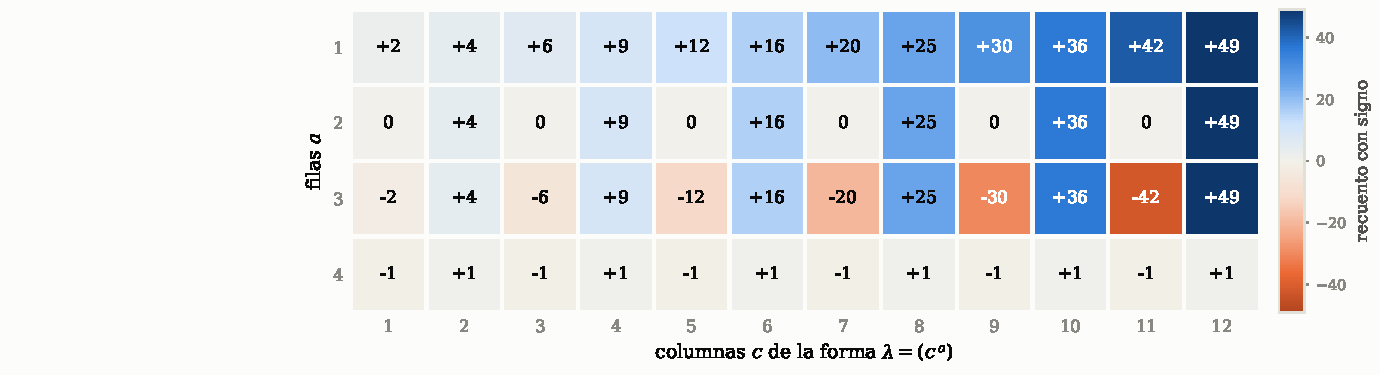
\includegraphics[width=\textwidth]{fig_signed_es.pdf}
\caption{Los recuentos con signo del Ejemplo \ref{ex:boxes}: el valor del Corolario \ref{cor:enum} en
$z=1$ y $t=2$ para las formas rectangulares $\lambda=(c^{\,a})$, esto es la $(-1)$-enumeración de
particiones planas en una caja $a\times(4-a)\times c$. Cada entrada es la forma cerrada
$\varepsilon_\lambda\,d_1d_2d_3/(2t^2)$, contrastada contra una enumeración directa de las tablas. La
fila $a=2$ se anula para $c$ impar y es un cuadrado perfecto para $c$ par.}
\label{fig:signed}
\end{figure}

La literatura de $(-1)$-enumeración calcula tales recuentos con signo, y conviene ser exacto en cómo,
porque la diferencia de aquí es estrecha. Kuperberg \cite{Kup02} pesa los objetos por $\pm1$
directamente. Eisenkölbl \cite{Eis07} especializa $x_i=(-1)^i$ en una identidad de funciones de Schur
del tipo que usó Stanley \cite{Sta86} ---identidad que allí se señala que es también
\cite[Cor.~7.3]{IOTZ06}--- y obtiene la $(-1)$-enumeración de las particiones planas
autocomplementarias con un lado impar. Ciucu y Krattenthaler evalúan los determinantes
correspondientes. En todos ellos el alfabeto es un número y no queda nada libre, que es el único
punto de diferencia: aquí el par recíproco mantiene viva una variable a lo largo del recuento con
signo. Eso lo hace el alfabeto, no un argumento nuestro.

En el mundo de las cintas hay un refinamiento de otra clase, y conviene decir cuál: los polinomios
LLT de Lascoux, Leclerc y Thibon \cite{LLT97} gradúan las tablas de cintas por un estadístico de
spin. Ese $q$ es una graduación añadida y no una letra, y el objeto que gradúa va indexado por una
tupla de formas; el parámetro de aquí es el del propio alfabeto y quien lo transporta es un solo
$s_\lambda$. Los dos refinan cosas distintas, y por eso enunciamos el punto de forma estrecha: es el
par recíproco, y no un estadístico, lo que mantiene viva una variable a través del recuento con
signo.

Una enumeración con signo que tiene fórmula de producto pide una involución que invierta el signo, y
el obstáculo es específico: la involución debe preservar $m_{t+1}-m_{t+2}$, o el parámetro libre no
se transporta, y ni los movimientos de Bender--Knuth ni el intercambio de una sola celda lo hacen.
La construcción de \cite{KumariThesis} de una involución sin puntos fijos que invierte el signo
sobre tablas semiestándar en un alfabeto emparejado por $\pm$, cuyo conjunto fijo son las tablas
embaldosables por dominós, sí tiene la propiedad requerida en su instancia $i=1$: toca solo celdas
que contienen $1$ o $2$, luego preserva $z^{m_3-m_4}$ e invierte $(-1)^{m_2}$. El producto triple
sobre el que tendría que aterrizar es el del Corolario \ref{cor:chars}, que en $t=2$ es sin más un
producto de tres caracteres $\mathfrak{sl}_2$, de modo que la biyección que falta es un enunciado de
Clebsch--Gordan. Esa es una mitad. La
otra es la cancelación a través de la partición del alfabeto, y en $t=2$ concierne a una única
familia de un parámetro. Por \eqref{eq:threestep} más abajo,
\[
s_\lambda(1,-1,z,\zb)=\sum_{\ell(\nu)\le2}s_{\lambda/\nu}(1,-1)\,\chi_{\nu_1-\nu_2}(z),
\]
y una involución que transporte el parámetro debe preservar $k=\nu_1-\nu_2$, porque ese es el índice
del carácter sobre el que se apoya su término. Para $k$ fijo las $\nu$ admisibles son exactamente
$(m+k,m)$ con $m\ge0$, de modo que esa cancelación es un enunciado sobre una sola palabra.

El tamaño de los términos es clásico. El teorema de Littlewood tiene forma sesgada ---$\varphi_t
s_{\lambda/\nu}$ se anula salvo que $\lambda/\nu$ sea embaldosable por $t$-cintas, y en otro caso es
un signo de cinta por un producto sobre el cociente---, debida a Macdonald \cite[p.~91]{Mac95} y
demostrada allí por la misma vía de Jacobi--Trudi que tomamos abajo; el caso en que $\nu$ es el
$t$-núcleo es de Farahat. En $t=2$ y sobre nuestro alfabeto da $\sigma_m\in\{0,\pm1\}$ de inmediato.
Lo que no es clásico es cómo se mueve el signo con $m$, y eso es lo que la involución necesita.

\begin{figure}[t]
\centering
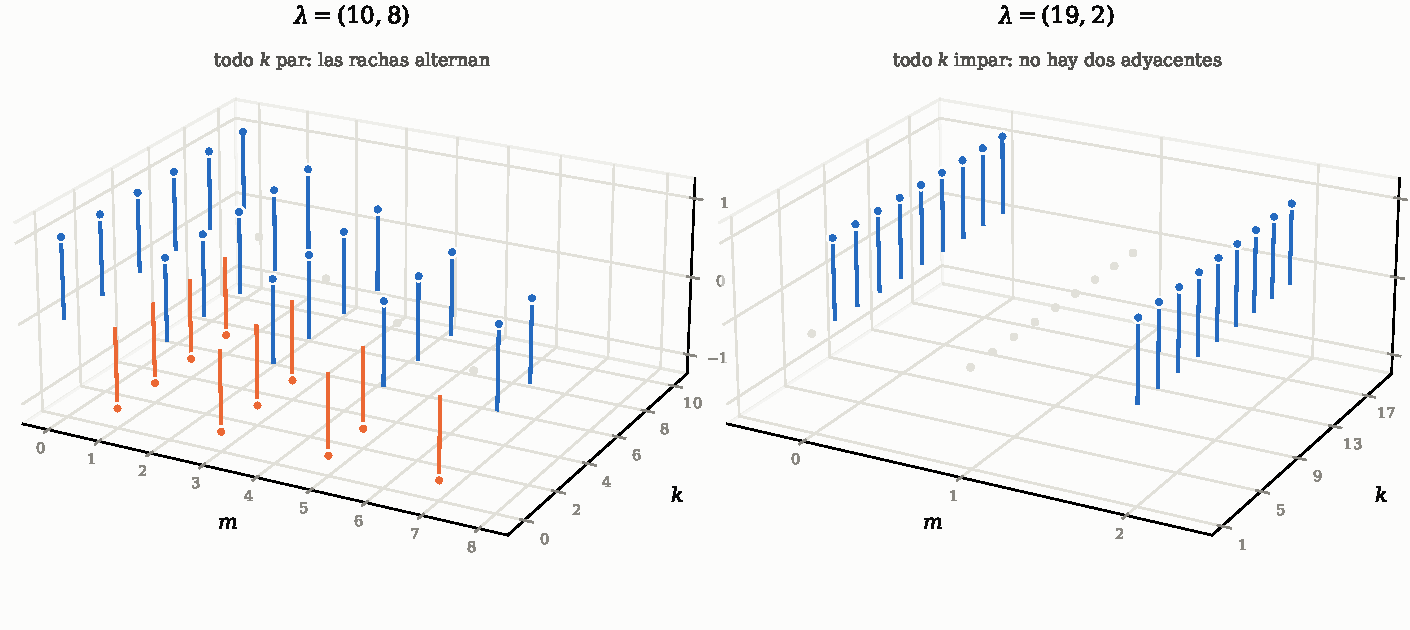
\includegraphics[width=\textwidth]{fig_runs_es.pdf}
\caption{La Proposición \ref{rem:involution}, dibujada. Para cada $k$ las $\nu$ admisibles son la
única familia $(m+k,m)$, y se representa $\sigma_m=s_{\lambda/(m+k,m)}(1,-1)$ frente a $m$ y $k$; los
puntos grises son los ceros. Toda barra tiene altura exactamente $\pm1$, que es la parte (i): los
términos forman un conjunto, luego la cancelación que pide la enumeración es un emparejamiento y no
algo con multiplicidad. A la izquierda todo $k$ es par y el color alterna a lo largo de cada racha,
que es la parte (iii) y lo que hace que $m\leftrightarrow m+1$ invierta el signo; donde una racha
acaba, la acaba un cero. A la derecha todo $k$ es impar y no hay dos términos no nulos contiguos,
que es la parte (ii): las rachas tienen longitud uno y no hay nada que cancelar.}
\label{fig:runs}
\end{figure}

\begin{proposition}[las rachas alternan]\label{rem:involution}
Sean $t=2$ y $k\ge0$, y sea $\sigma_m=s_{\lambda/(m+k,m)}(1,-1)$ para $m\ge0$. Entonces
\begin{enumerate}
\item[\rm(i)] $\sigma_m\in\{0,\pm1\}$ --- esta parte es de Macdonald y no nuestra;
\item[\rm(ii)] si $k$ es impar, no hay dos $\sigma_m$ consecutivos no nulos;
\item[\rm(iii)] si $\sigma_m$ y $\sigma_{m+1}$ son ambos no nulos, entonces
$\sigma_{m+1}=-\sigma_m$.
\end{enumerate}
En consecuencia, emparejar $m$ con $m+1$ dentro de cada racha maximal de $\sigma$ no nulos
consecutivos es una involución que invierte el signo, y $\sum_m\sigma_m$ es el recuento con signo de
las rachas de longitud impar.
\end{proposition}

Las tres partes se ven a la vez en la Figura \ref{fig:runs}: las alturas de las barras son la parte
{\rm(i)}, los huecos del panel impar son la parte {\rm(ii)}, y la alternancia del color a lo largo de
cada racha es la parte {\rm(iii)}.

\begin{proof}
Escribamos $\beta_i=\lambda_i-i$ y $c_j=\nu_j-j$, y tomemos la matriz de Jacobi--Trudi de
$s_{\lambda/\nu}$ con $n\ge\ell(\lambda)$ filas. Como $h_j(1,-1)=1$ para $j\ge0$ par y $0$ en otro
caso,
\begin{equation}\label{eq:betaJT}
M_{ij}=\bigl[\beta_i\ge c_j\bigr]\cdot\bigl[\beta_i\equiv c_j \bmod 2\bigr],\qquad
\sigma_m=\det M .
\end{equation}
El segundo factor dice que la columna $j$ está soportada en las filas de una sola clase de paridad,
la de $c_j$; y como $\beta_1>\dots>\beta_n$, dentro de esa clase el primer factor recorta un
\emph{segmento inicial}. Ordenando las filas por clase de paridad, $M$ queda diagonal por bloques,
de modo que es singular salvo que cada clase lleve tantas columnas como filas tiene, y dentro de una
clase es la escalera $\bigl[\,\text{el rango de }i\text{ en su clase}\le\ell_j\bigr]$ de las
longitudes $\ell_j$. Esa escalera es singular si dos longitudes coinciden o alguna es $0$, y en otro
caso las longitudes son una permutación de $1,\dots,e$ y su determinante es el signo de esa
permutación. Esto da (i), que en este caso es \cite[p.~91]{Mac95}; lo rededucimos porque la forma
$\beta$ \eqref{eq:betaJT} es lo que sostiene (ii) y (iii).

Para $\nu=(m+k,m)$ se tiene $c_1=m+k-1$, $c_2=m-2$ y $c_j=-j$ para $j\ge3$. Luego $c_1-c_2=k+1$, y
pasar de $m$ a $m+1$ sube $c_1$ y $c_2$ en uno y deja las demás columnas quietas: cambian de clase
de paridad exactamente las dos primeras.

Si $k$ es impar entonces $c_1\equiv c_2$, así que las columnas $1$ y $2$ están en la misma clase y
ambas la abandonan. El número de columnas de esa clase cambia en dos mientras que su número de filas
no, de modo que a lo sumo uno de $\sigma_m$, $\sigma_{m+1}$ puede ser no nulo, que es (ii).

Si $k$ es par entonces $c_1\not\equiv c_2$ y las dos columnas intercambian clase. Supongamos que
ambos son no nulos. En la clase de $c_1$ las columnas son la columna $1$ junto con un conjunto de
columnas $j\ge3$ que no se mueve; por (i) las longitudes son una permutación de $1,\dots,e$ antes y
después, y las columnas fijas aportan las mismas a ambas, luego la longitud que trae la columna $2$
es la que se llevó la columna $1$ ---y simétricamente en la otra clase. Cada clase ve por tanto las
mismas longitudes en el mismo orden de columnas, y los dos determinantes de bloque no cambian. Lo
que sí cambia es la baraja que separa las dos clases de columnas: las columnas $1$ y $2$ son
contiguas e intercambian pertenencia, lo que altera el número de inversiones de esa baraja en
exactamente uno. Luego $\sigma_{m+1}=-\sigma_m$, que es (iii).
\end{proof}

\begin{remark}[el signo de aquí es el signo del Teorema \ref{thm:main}]\label{rem:onesign}
Escribamos $\sigma_\nu$ para la permutación de la \S\ref{sec:background} asociada a una partición
$\nu$: la que ordena $\beta$ por clase de residuos, y que la Proposición \ref{rem:sign} coloca
dentro de $\varepsilon_\lambda$. Los términos de la Proposición \ref{rem:involution} son valores de
ese mismo signo. En efecto, $\sigma_m$ se anula salvo que $\core_2(\lambda)=\core_2(\nu)$ y ambas
componentes del $2$-cociente sesgado sean tiras horizontales, y vale
$\sgn(\sigma_\lambda)\sgn(\sigma_\nu)$ cuando no se anula ---siendo la identidad
$\sgn(\sigma_\lambda)\sgn(\sigma_\nu)=(-1)^{\sum_B\mathrm{ht}(B)}$ el signo de cintas de
\cite[p.~91]{Mac95} escrito como signo de ordenación, que es
\cite[Lema 6.3]{KumariThesis}. Las partes {\rm(ii)} y {\rm(iii)} son
entonces un único enunciado sobre $\sigma_\nu$ solo: al pasar $\nu=(m+k,m)$ a $(m+k+1,m+1)$,
$\sgn(\sigma_\nu)$ cambia de signo si $k$ es par y es constante si $k$ es impar. Así que la
permutación que lleva el signo del teorema principal es la permutación que hace alternar la
involución de esta sección; las dos mitades del artículo están firmadas por un mismo objeto.
\end{remark}

El emparejamiento es una biyección de tablas y no solo de términos, que es lo que transporta el
parámetro. Una tabla semiestándar de forma $(a,b)$ en las letras $3,4$ tiene segunda fila $4^{\,b}$
y primera fila $3^{\,p}4^{\,a-p}$ con $b\le p\le a$, de peso $z^{2p-a-b}$; añadirle una primera
columna $\left(\begin{smallmatrix}3\\4\end{smallmatrix}\right)$ la lleva a la tabla de forma
$(a+1,b+1)$ con $p+1$ en lugar de $p$, y $2(p+1)-(a+1)-(b+1)=2p-a-b$, de modo que $m_3-m_4$ se
preserva exactamente. Componer eso con la Proposición \ref{rem:involution} empareja los términos del
Corolario \ref{cor:enum} del modo que la enumeración pide.

Una mitad no es nuestra, y decimos cuál. La Proposición \ref{rem:involution} despacha la cancelación
a través de $\nu$; la cancelación \emph{dentro} de cada $s_{\lambda/\nu}(1,-1)$ es
\cite{KumariThesis}, y las dos encajan. Allí, con $n=1$, el alfabeto es $(x,-x)$ y el peso de un
llenado de dos letras es $(-1)^{c_2}$, que es $\sigma_m$; la involución
\cite[Lema 2.18]{KumariThesis} es libre de puntos fijos sobre los llenados \emph{no cubribles}, de
modo que la suma se reduce a los cubribles, que el \cite[Lema 2.16]{KumariThesis} pone en
correspondencia con tablas de dominó. Lo que hace utilizable la reducción aquí es el
\cite[Lema 2.14]{KumariThesis}: la paridad del número de dominós verticales no depende de la tabla,
luego toda superviviente lleva el mismo signo y $\sigma_m=\pm\#\{\text{llenados cubribles}\}$. Con la
parte (i), eso obliga al recuento a ser a lo sumo uno, así que el conjunto fijo es un único llenado
cuando $\sigma_m\ne0$ y vacío en otro caso ---comprobado directamente sobre las $1134$ formas
sesgadas con a lo sumo cuatro filas y $|\lambda|\le10$, donde los dos recuentos coinciden sin
excepción.

En $t=2$ existe por tanto la involución que la enumeración pide: cancelar dentro de cada $\nu$ por
el \cite[Lema 2.18]{KumariThesis}, emparejar lo que queda a través de $\nu$ por la Proposición
\ref{rem:involution}, y transportar el parámetro con la columna
$\left(\begin{smallmatrix}3\\4\end{smallmatrix}\right)$. Sus puntos fijos son un llenado por cada
racha de longitud impar, y el Corolario \ref{cor:enum} los cuenta. La construcción es de Kumari; el
ensamblaje es nuestro.

%======================================================================
\section{La factorización está aislada}\label{sec:sharp}

Una factorización solo es un resultado si no es especialización de otra conocida, y solo es un
resultado \emph{nítido} si el alfabeto no admite deformación. Eso no lo demostramos en general. Lo
que hacemos es probar cuatro deformaciones de \eqref{eq:object}, y las cuatro destruyen el producto.

La evidencia de esta sección es computacional, y así la etiquetamos: ninguna de (D1)--(D4) es un
teorema, y en particular no demostramos ningún resultado de imposibilidad. Lo que afirmamos es que la
identidad \eqref{eq:main} es falsa para cada alfabeto deformado, cosa que zanja un solo
contraejemplo, y damos recuentos para indicar cuán lejos está de ser cierta.

\begin{itemize}
\item[\rm(D1)] \emph{Más pares recíprocos.} Para
$s_\lambda(\zt,z_1,z_1^{-1},\dots,z_r,z_r^{-1})$
la ley de producto del Teorema \ref{thm:main} ya falla en $r=2$: en el rango calculado los valores
típicos llevan un factor irreducible grande, y los únicos
factores que se observa que se desprendan son binomios en las variables rotadas $z_1z_2$ y $z_1z_2^{-1}$, esto es,
los acoplamientos entre las cargas $u(1)$ de los pares. Lo que sí sobrevive es el \emph{lugar de
anulación}: en $t=2$ sobrevive a todo $r$ y el Teorema \ref{conj:crit} lo determina por completo,
mientras que para $t$ y $r$ arbitrarios el Teorema \ref{thm:suff} da un criterio suficiente uniforme
y la Conjetura \ref{conj:general} es el recíproco. Con esta evidencia el producto parece un accidente
de rango uno y la anulación la parte que generaliza; la primera mitad de esa frase es la Conjetura
\ref{conj:rank2} y sólo la segunda es un teorema.
\item[\rm(D2)] \emph{Más variables en la órbita.} Para
$s_\lambda(X,\zeta X,\dots,\zeta^{t-1}X,z,z^{-1})$ la ley de producto ya falla en $|X|=n=2$. Con $t=2$,
$n=2$ el valor para $\lambda=(2)$ es $(x^2z^2+y^2z^2+z^4+z^2+1)/z^2$, irreducible sobre $\mathbb Q$;
para $\lambda=(2,2)$ es $(x^2+y^2+z^2)(x^2z^2+y^2z^2+1)/z^2$, dos factores en lugar de tres; y para
$\lambda=(3,1)$ es de nuevo irreducible. En cambio, suprimido el par, el mismo alfabeto obedece
\cite[Teorema 2.3]{AK25}: $s_{(2)}(x,y,-x,-y)=x^2+y^2$ y $s_{(2,2)}(x,y,-x,-y)=(x^2+y^2)^2$.
\item[\rm(D3)] \emph{La órbita sustituida por una clase lateral.} Para $\zeta'\zt$ con
$\zeta'=e^{\pi i/t}$, las potencias impares de una raíz $2t$-ésima primitiva de la unidad ---el
torcimiento de \cite[\S3]{AK25}, y para $t$ par el conjunto completo de raíces $2t$-ésimas primitivas
estudiado en \cite{HI24}--- la identidad falla, criterio de anulación incluido.
\item[\rm(D4)] \emph{El par recíproco sustituido por un par libre.} $s_\lambda(\zt,x,y)$ resultó
irreducible en todos los casos que calculamos. No afirmamos nada fuera de ese rango.
\end{itemize}

Recuentos para (D3) y (D4), sobre $t=2,\dots,6$ y $|\lambda|\le10$: la identidad se cumple en los
$600$ casos para \eqref{eq:object}, en $383$ de $600$ para (D3) y en $200$ de $600$ para (D4). El
contraste es por tanto capaz de fallar, que es la razón de citar la primera fila.

Una sola lectura de la demostración explica las cuatro. Partiendo el alfabeto y aplicando el Teorema
\ref{thm:LR} a la mitad congelada se obtiene, para cualquier alfabeto libre $B$,
\begin{equation}\label{eq:threestep}
s_\lambda(\zt\cup B)=\sum_{\nu}s_{\lambda/\nu}(\zt)\,s_\nu(B)=\sum_\nu\varepsilon_\nu\,s_\nu(B),
\qquad \varepsilon_\nu\in\{0,\pm1\},
\end{equation}
siendo los coeficientes signos de cinta: que la evaluación sesgada $s_{\lambda/\nu}(\zt)$ sea $0$ o
un signo de cinta es la forma sesgada del Teorema \ref{thm:LR}, debida a Macdonald
\cite[p.~91]{Mac95}. Ahora bien, $B=(z,z^{-1})$ tiene exactamente dos letras y
son recíprocas, luego $s_\nu(B)=\chi_{\nu_1-\nu_2}(z)$ es un \emph{único} carácter
$\mathfrak{sl}_2$ que depende de una sola diferencia, y la suma corta con signos colapsa. El primer
paso exige que la mitad congelada sea una órbita completa, pues el Teorema \ref{thm:LR} necesita que
las filas toquen cada clase de residuos exactamente; una clase lateral no lo hace, y eso es (D3). El
segundo paso exige que la mitad libre sea exactamente un par recíproco: un par libre tiene
$\det=xy$ y se acopla a las dos cargas centrales, y eso es (D4), mientras que agrandar la mitad libre
---con más pares, o con más variables en la órbita, lo que agranda $\nu$--- hace que $s_\nu(B)$ deje
de ser un único carácter y que la suma deje de colapsar, y eso es (D1) y (D2). \emph{Los cuatro
fallos son una sola condición vista desde cuatro lados.}

\begin{remark}
Equivalentemente: el par recíproco aporta exactamente \emph{un} acoplamiento, el término cruzado
$d_3$, porque $\det=1$ le impide ver por separado las dos cargas centrales. Por eso hay tres factores
y no dos, y las factorizaciones de Ayyer--Kumari, que son productos sobre componentes del cociente
sin acoplamiento alguno, son el caso en que esa aportación está ausente.
\end{remark}

\begin{remark}[una lectura teórico-representacional]\label{rem:twining}
El alfabeto \eqref{eq:object} es cerrado bajo inversión, luego es un elemento del toro de $O(N)$, y
su determinante es $(-1)^{t+1}$. Para $t$ par está por tanto en la componente no identidad, donde un
carácter es un carácter \emph{twining}; la identidad que calcula tales caracteres por plegado se debe
a Jantzen \cite{Jantzen} y, en la forma más próxima a esta, a Kumar--Lusztig--Prasad \cite{KLP},
siendo el álgebra plegada relevante el álgebra órbita. Nuestra restricción es reducible, de modo que
se llega a ella desde la suya con un paso de teoría de Clifford. Lo registramos porque
Ciucu--Krattenthaler \cite{CK09} escribieron que no podían ofrecer una interpretación
teórico-representacional de sus factorizaciones, y \cite{AB19} y \cite{AK25} registran que sigue
faltando; la lectura de aquí es de esa clase. El mecanismo es enteramente suyo, y la demostración
anterior no lo usa. El Lema \ref{lem:AtoSp} concreta esa lectura para el alfabeto \eqref{eq:psir},
donde el álgebra plegada es $C_r$ y el carácter twining es un carácter simpléctico sin más.
\end{remark}

%======================================================================
\section{El lugar de anulación sobrevive a todo $r$}\label{sec:zeros}

Esta sección está más allá de la factorización, y se lee distinto de las siete anteriores. Aquéllas
demuestran enunciados sobre una identidad; ésta pregunta qué queda cuando la identidad ya no está, y
la respuesta es un lugar geométrico y no una fórmula ---demostrado en un sentido para todo $r$, y en
el otro solo hasta donde hemos podido llegar. El cambio de registro es el asunto que cambia, no el
listón.

Por (D1), el producto del Teorema \ref{thm:main} no sobrevive a un segundo par recíproco. Su
\emph{lugar de anulación} sí, y para todo $r$ admite forma cerrada. Escribamos
\begin{equation}\label{eq:psir}
\Psi_r(\lambda)\;:=\;s_\lambda(1,-1,z_1,\bar z_1,\dots,z_r,\bar z_r),\qquad N=2r+2,
\end{equation}
de modo que $\Psi_1$ es \eqref{eq:object} en $t=2$. En toda esta sección $\lambda$ se completa con
ceros hasta tener exactamente $N$ partes, $\beta=\beta(\lambda)$ es su conjunto beta y $E$ y $O$ son
sus entradas pares e impares. Diremos que $\lambda$ es \emph{autocomplementaria de anchura $w$} si
$\lambda_i+\lambda_{N+1-i}=w$ para todo $i$, en cuyo caso $w=\lambda_1+\lambda_N$. Las dos
condiciones que gobiernan la sección son
\begin{equation}\label{eq:branches}
\boxed{\;\;
\underbrace{|E|\in\{0,N\}}_{\text{rama (a)}}
\qquad\qquad
\underbrace{\lambda_i+\lambda_{N+1-i}=w\ \ \text{para todo }i,\ \ w\ \text{impar}}_{\text{rama (b)}}
\;\;}
\end{equation}
La rama (a) dice que el conjunto beta tiene paridad constante; la rama (b), que $\lambda$ es
autocomplementaria de anchura impar.

Enunciamos las cuatro afirmaciones por separado, porque no están demostradas en la misma medida y un
único bicondicional lo ocultaría.

\begin{theorem}[las dos ramas]\label{thm:zeros}
Para todo $r\ge1$ y toda $\lambda$: si se cumple la rama {\rm(a)} o la rama {\rm(b)}, entonces
$\Psi_r(\lambda)=0$.
\end{theorem}

\begin{corollary}\label{cor:sizes}
Si $\lambda$ es autocomplementaria de anchura impar $w$, entonces $|\lambda|=w(r+1)$. En particular
la rama {\rm(b)} solo puede darse para $|\lambda|\equiv r+1 \pmod{2(r+1)}$, y un tamaño fuera de esa
progresión no necesita más comprobación.
\end{corollary}

\begin{proof}
Sumar $\lambda_i+\lambda_{N+1-i}=w$ sobre $i$ cuenta $|\lambda|$ dos veces, luego
$2|\lambda|=wN=w(2r+2)$.
\end{proof}

La progresión se ve en la Figura \ref{fig:zeros}, y merece la pena dejar constancia de que el
enunciado análogo para el lugar entero es falso: la rama {\rm(a)} no está confinada a ella, y por eso
la condición hay que leerla sobre la rama {\rm(b)} sola.

\begin{figure}[!ht]
\centering
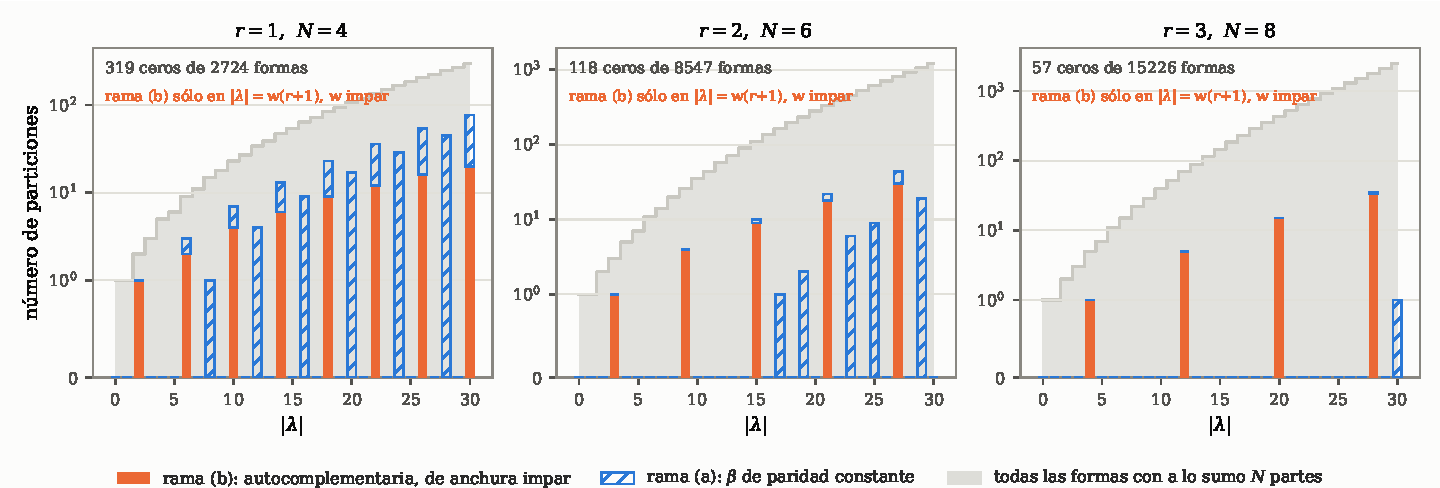
\includegraphics[width=\textwidth]{fig_zeros_es.pdf}
\caption{El lugar de anulación del Teorema \ref{thm:zeros}, contado en lugar de dibujado. Para cada
tamaño $|\lambda|$ las barras dan el número de particiones con a lo sumo $N$ partes que se anulan,
separadas por rama; el escalón sombreado es el número total de formas de ese tamaño, en el mismo eje,
de modo que la rareza del lugar se ve y no se afirma. Los tamaños que llevan la rama (b) son
exactamente los múltiplos $w(r+1)$ con $w$ impar, por el Corolario \ref{cor:sizes}; la rama (a) ocupa
otros tamaños y necesita que el conjunto beta se salte una paridad por completo, razón por la cual
está ausente en $|\lambda|$ pequeño en cuanto $N$ crece.}
\label{fig:zeros}
\end{figure} Conviene dejar constancia de que el enunciado
análogo para todo el lugar de anulación es falso: la rama (a) no está confinada a esa progresión, y
por eso la condición hay que leerla de la rama (b) sola.

\begin{theorem}[un par]\label{thm:r1}
Para $r=1$ vale también el recíproco: $\Psi_1(\lambda)=0$ solo si se cumple {\rm(a)} o {\rm(b)}.
\end{theorem}

\begin{theorem}[dentro del rango de Littlewood]\label{thm:stable}
Para todo $r$ y toda $\lambda$ con $\ell(\lambda)\le N/2$ vale el recíproco. Equivalentemente, en ese
rango $\Psi_r(\lambda)=0$ si y solo si $\lambda=(k^{\,N/2})$ con $k$ impar.
\end{theorem}

\begin{remark}[los rectángulos son donde se detienen los argumentos generales]
Vale la pena advertir que los dos sitios donde falla un argumento general de este artículo son
rectángulos, a dos alturas distintas y por dos razones distintas. A altura $N/2$ un rectángulo impar
es autocomplementario de anchura impar, luego se anula; por el Teorema \ref{thm:stable} son las
únicas formas del rango de Littlewood que lo hacen, y en la demostración son precisamente aquellas
para las que no se puede construir el testigo asociado. A altura completa el objeto no se anula, sino
que degenera en sentido contrario: $s_{(c^{\,N})}(x)=(x_1\cdots x_N)^{c}$ es un monomio, de modo que
sobre cualquier alfabeto $A$ el valor es $\det(A)^{c}$ y de la forma no sobrevive nada ---que con
$t=2$ es el caso {\rm(i)} de la Proposición \ref{prop:rect}, el único allí en el que la paridad de
$c$ no interviene---. Entre ambas alturas el argumento genérico se aplica sin cambios. Los
rectángulos no son una molestia que haya que tratar caso por caso: son el borde de la forma, y cada
uno de los dos extremos rompe una hipótesis distinta ---el primero la existencia de un testigo, el
segundo la no degeneración del triple de intervalos---.
\end{remark}

\begin{theorem}[el criterio en general]\label{conj:crit}
Para todo $r$ y toda $\lambda\in\PP_N$, $\Psi_r(\lambda)=0$ si y solo si se cumple {\rm(a)} o
{\rm(b)}.
\end{theorem}

\noindent Demostrado al final de la \S\ref{sec:zeros}, módulo el Teorema \ref{thm:PvW}.

Los Teoremas \ref{thm:zeros}--\ref{thm:stable} se demuestran en las
\S\S\ref{sec:brancha}--\ref{sec:conv}, y el Teorema \ref{conj:crit} --- el criterio para todo
$r$ --- al final de esta sección, por una vía independiente de los tres. Lo enunciamos aparte por dos
razones. Es el único resultado del artículo que se apoya en algo ajeno, el Teorema
\ref{thm:PvW}; y las dos vías que llevan a él no son la misma vía. La de Littlewood lo reduce, en la
\S\ref{sec:unstable}, a un único enunciado de existencia, y esa reducción no se completa: el rango
$\ell(\lambda)>N/2$ es exactamente donde la regla de restricción deja de aplicarse y, aunque el
Lema \ref{lem:AtoSp} resuelve allí los valores, el enunciado sobre los coeficientes no --- el
certificado que propusimos para él falla, por la Proposición \ref{conj:iso}. El argumento extremal
de las \S\S\ref{sec:extremal} y \ref{sec:rigidity} no entra en ese rango en absoluto: trabaja en
la filtración por grados del numerador y no se cruza jamás con un coeficiente de Littlewood.

Leído sobre el grupo y no sobre el alfabeto, el mismo teorema describe una propiedad de rigidez, y lo
enunciamos aparte porque es la forma en que lo querría alguien de teoría de representaciones. La
traducción no es nuestra ni es nueva: que una representación de $O(N)$ sea estable por $\det$
exactamente cuando su carácter se anula fuera de la componente identidad es elemental, y que eso sea
la condición $m_\nu=m_{\nu^{*}}$ sobre los asociados de Littlewood \cite{Lit50} es clásico. El
corolario reclama por tanto exactamente lo que reclama el Teorema \ref{conj:crit}, y nada más.

\begin{corollary}[rigidez frente al giro por el determinante]\label{cor:dettwist}
Sean $N=2r+2$ y $\lambda\in\PP_N$, y sea $V_\lambda$ el $GL(N)$-módulo polinómico irreducible de peso
máximo $\lambda$. Entonces
\[
V_\lambda\big|_{O(N)}\;\cong\;V_\lambda\big|_{O(N)}\otimes\det
\]
si y solo si $\beta(\lambda)$ tiene paridad constante, o $\lambda$ es autocomplementaria de anchura
impar. Equivalentemente: \eqref{eq:branches} clasifica exactamente los $GL(N)$-módulos polinómicos
irreducibles cuya restricción a $O(N)$ es estable por el carácter del grupo de componentes.
\end{corollary}

\begin{proof}
En característica $0$ un $O(N)$-módulo de dimensión finita es semisimple y queda determinado por su
carácter, así que para $W=V_\lambda|_{O(N)}$ se tiene $W\cong W\otimes\det$ si y solo si
$\chi_W=\chi_{W\otimes\det}$. Esos dos caracteres coinciden automáticamente en la componente
identidad, y en la otra $\chi_{W\otimes\det}=-\chi_W$; luego la condición es que $\chi_W$ se anule en
$O(N)^{-}$. Todo elemento \emph{semisimple} de $O(N)^{-}$ es conjugado a uno de espectro
$(1,-1,z_1^{\pm1},\dots,z_r^{\pm1})$, que es el alfabeto de \eqref{eq:psir}; y como los semisimples
son densos en $O(N)^{-}$ y $\chi_W$ es regular, anularse en ese toro es anularse en toda la
componente. La condición es por tanto $\Psi_r(\lambda)\equiv0$, y el Teorema \ref{conj:crit} es el
criterio. El diccionario entre las dos lecturas es la expansión por asociados de Littlewood, recordada
en la \S\ref{sec:conv}.
\end{proof}

\noindent El crédito se reparte exactamente igual que en el Teorema \ref{conj:crit}, y conviene
repetirlo aquí porque el lenguaje de grupos puede hacer que un enunciado conocido parezca nuevo. Que
las dos familias \eqref{eq:branches} \emph{sean} estables por $\det$ no es nuestro: en el extremo de
la familia, la primera es de Karmakar \cite[Teorema 4.1(A)]{Kar24}, y la segunda es la complementación
sobre la familia de índices de Ayyer y Behrend \cite{AB19}, como recoge \eqref{eq:compl}. Lo que el
Teorema \ref{conj:crit} añade, y es todo lo que añade, es que no hay ninguna más.

\begin{remark}[lo que el núcleo ve, y lo que no]\label{rem:core}
La rama (a) es una condición sobre el núcleo, y sencilla: con un número $N$ fijo de números beta, el
perfil de residuos determina $\core_t(\lambda)$ ---es la coordenada de Garvan--Kim--Stanton
\cite{GKS90}---, de modo que toda condición sobre el perfil lo es sobre el núcleo. No es, sin
embargo, la anulación del núcleo sino su extremo opuesto: en $t=2$ la rama (a) dice
\[
\core_2(\lambda)=(N-1,N-2,\dots,1)\qquad\text{o}\qquad\core_2(\lambda)=(N,N-1,\dots,1),
\]
los dos $2$-núcleos más grandes que admiten $N$ números beta, mientras que
$\core_2(\lambda)=\varnothing$ es el perfil equilibrado. La rama (b) no mueve ni el perfil ni el
núcleo, y por tanto le es invisible. En consecuencia $\core_2$ \emph{no} determina si $\Psi_r$ se
anula, y el testigo más pequeño es el propio núcleo vacío: entre las formas con
$\core_2(\lambda)=\varnothing$ en $r=1$,
\[
(1,1),\ (3,3),\ (2,2,1,1),\ \dots\quad\text{se anulan, y}\quad
\varnothing,\ (2),\ (1^4),\ \dots\quad\text{no,}
\]
y el mismo corte ocurre en $r=2$ y $r=3$, allí también en las clases de núcleo $(1)$, $(2,1)$ y
$(3,2,1)$: sobre los rangos de la \S\ref{sec:verif} hay cinco clases de núcleo que llevan ambos
comportamientos, y el perfil determina el núcleo sin ninguna colisión sobre $260$ perfiles con
$t\le5$. No puede existir, pues, ninguna reformulación del Teorema \ref{thm:zeros} en términos de
$\core_2(\lambda)$: el criterio necesita la forma y no solo su núcleo. Leídos contra el Teorema
\ref{thm:LR}, donde el núcleo vacío es exactamente lo que decide, los dos criterios discrepan en
ambas direcciones ---$(1,1)$ tiene $2$-núcleo vacío y $\Psi_1=0$, mientras que $(1)$ tiene
$2$-núcleo no vacío y $\Psi_1\ne0$.
\end{remark}

La familia de índices de (b) no es nueva: es precisamente la que Ayyer y Behrend destacan
\cite[observación tras el Teo.~3]{AB19}, junto con la obstrucción de paridad que registran allí ---una
partición no puede ser autocomplementaria en un rectángulo $a\times b$ con $a$ y $b$ ambos impares, y
aquí $a=N$ es par, luego el caso admisible es $b=w$ impar. Lo que sus teoremas dicen de esas formas es
que el carácter \emph{factoriza}; allí el alfabeto lleva el punto fijo $+1$ y tiene determinante $+1$.
El nuestro lleva $+1$ y $-1$, y tiene determinante $-1$.

\keybox{Sobre la \emph{misma} familia de formas, el alfabeto de determinante $+1$ hace que el
carácter factorice y el de determinante $-1$ hace que se anule. Una letra separa una factorización de
una aniquilación, y quien decide es el determinante del alfabeto; la identidad \eqref{eq:compl} de
más abajo es donde ocurre la separación.}


\subsection{Rama (a): el alfabeto al cuadrado}\label{sec:brancha}

Esta rama es de Karmakar, en el extremo. \cite[Teorema 4.1(A)]{Kar24} evalúa un carácter de
$\mathrm{GL}(n,\CC)$ en $C_{n-k,k}=(1,\dots,1,-1,\dots,-1)$ y da
$\chi_\lambda(C_{n-k,k})=0$ cuando $\#\eta_0(\lambda)>n-k$, donde su
$\eta_i(\lambda)=\{a\in\lambda+\rho: a\equiv i \bmod 2\}$ es exactamente la partición de
$\beta(\lambda)$ en $E$ y $O$ que usamos aquí; en $k=1$, tras su normalización por el carácter
determinante, eso es la rama (a). El argumento de una línea que sigue se incluye porque es el que
reutiliza el resto de la sección, no porque sea nuevo.

\begin{proof}[Demostración del Teorema \ref{thm:zeros}, rama {\rm(a)}]
Sea $A=\{1,-1,z_1,\bar z_1,\dots\}$. Si $\beta=2\gamma$, entonces
$\det(a^{\beta_j})_{a\in A}=\det\big((a^2)^{\gamma_j}\big)_{a\in A}$, y si $\beta=2\gamma+1$ ocurre lo
mismo tras extraer $\prod_{a\in A}a$. En ambos casos el bialternante factoriza a través del alfabeto
al cuadrado $A^2=\{1,1,z_1^{2},\bar z_1^{2},\dots\}$, en el que la letra $1$ aparece dos veces porque
$1^2=(-1)^2$. Hay dos filas iguales.
\end{proof}

\subsection{Rama (b): una torsión por el determinante, y autodualidad}

\begin{proof}[Demostración del Teorema \ref{thm:zeros}, rama {\rm(b)}]
Sea $\hat\lambda$ el complementario de $\lambda$ en la caja $w\times N$, leído del revés. En
conjuntos beta, $\beta(\hat\lambda)=c-\beta(\lambda)$ recorrido en sentido inverso, con $c=w+N-1$, y
$\hat\lambda$ es el peso máximo de $V_\lambda^{*}\otimes\det^{\,w}$ como $\mathrm{GL}(N)$-módulo. Si
$\lambda=\hat\lambda$, entonces $V_\lambda\cong V_\lambda^{*}\otimes\det^{\,w}$. Restrinjamos a
$O(N)$: toda representación de $O(N)$ es autodual, luego
$V_\lambda|_{O(N)}\cong V_\lambda^{*}|_{O(N)}\cong V_\lambda|_{O(N)}$, de donde
\[
V_\lambda|_{O(N)}\;\cong\;V_\lambda|_{O(N)}\otimes\det^{\,w}.
\]
El alfabeto \eqref{eq:psir} es un elemento del toro de la componente $\det=-1$, así que para $w$
impar la torsión es por $\det$ mismo y el carácter se anula ahí. Para $w$ par, $\det^{\,w}$ es
trivial y el argumento no da nada: por eso la paridad de $w$ no es un adorno.
\end{proof}

Equivalentemente, y esto es el cálculo en lugar de la representación, la identidad de complementación
estándar da
\begin{equation}\label{eq:compl}
s_{\hat\lambda}(A)\;=\;\Big(\textstyle\prod_{a\in A}a\Big)^{c}\,(-1)^{\binom{N}{2}}(-1)^{r}\,
s_\lambda(A)\;=\;(-1)^{c}\,(-1)\,s_\lambda(A),
\end{equation}
usando que $A$ es cerrado por inversión ---$A^{-1}$ es $A$ con los $r$ pares recíprocos
transpuestos, lo que aporta $(-1)^r$--- y que $\prod_{a\in A}a=-1$. Con $c$ par esto se lee
$s_{\hat\lambda}=-s_\lambda$, y una forma autocomplementaria queda aniquilada. La rama (b) del
Teorema \ref{thm:zeros} es por tanto un corolario de dos líneas de una identidad de manual sobre una
familia de índices conocida, y no la reclamamos como nada más. La Figura \ref{fig:involution} dibuja
el emparejamiento que hace la identidad, y a su lado la misma forma con una caja movida, donde el
emparejamiento se rompe; el contenido de la sección es el recíproco.

\subsection{El recíproco}\label{sec:conv}

\begin{figure}[t]
\centering
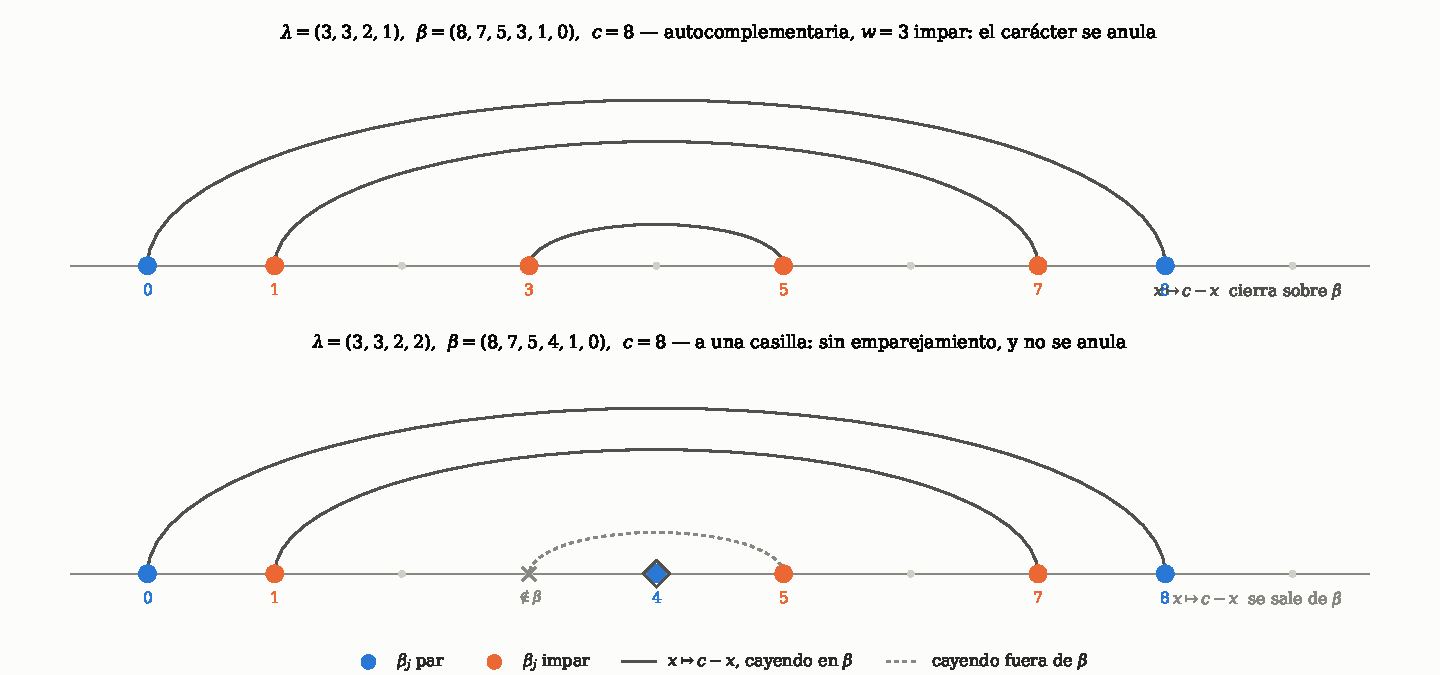
\includegraphics[width=\textwidth]{fig_involution_es.pdf}
\caption{Por qué la autocomplementariedad mata el carácter. Al desarrollar por las dos filas
congeladas quedan términos indexados por pares $(e,o)$ con $e\in E$, $o\in O$, y la reflexión
$x\mapsto c-x$ actúa sobre ellos. Arriba, una forma autocomplementaria de anchura impar: todo arco
cae dentro de $\beta$ y une entradas de igual paridad, porque $c$ es par. Abajo, la misma forma con
una caja movida: el arco $5\mapsto3$ se sale de $\beta$, así que no hay emparejamiento y nada se
cancela. El rombo marca el punto fijo de la reflexión, que no puede darse dentro de un par de
paridades opuestas ---y ésa es la razón de que la involución sea libre.}
\label{fig:involution}
\end{figure}

\begin{proof}[Demostración del Teorema \ref{thm:r1}]
Pongamos $c_\ast=z+\bar z$ y definamos $S_n$ por $S_0=0$, $S_1=1$, $S_{n+1}=c_\ast S_n-S_{n-1}$, de
modo que $\deg_{c_\ast}S_n=n-1$ y $S_{-n}=-S_n$; el valor $S_{-1}=-1$ se usa siempre que
$\beta_N=0$. Como $\Phi_A=(x^2-1)(x^2-c_\ast x+1)$, un polinomio $P$ soportado en $\beta$ es
divisible por $\Phi_A$ exactamente cuando $P(1)=P(-1)=0$ y $P\equiv0$ módulo $x^2-c_\ast x+1$.
Separando $P(\pm1)$ por paridad y reduciendo $x^n\equiv S_nx-S_{n-1}$, la admisibilidad se convierte
en la singularidad de la matriz $4\times4$ con filas $[\beta_j\ \mathrm{par}]$,
$[\beta_j\ \mathrm{impar}]$, $S_{\beta_j}$, $S_{\beta_j-1}$. Desarrollando por las dos filas de
paridad y usando la identidad de d'Ocagne \cite{Doc} para esta recurrencia,
\begin{equation}\label{eq:docagne}
S_bS_{b'-1}-S_{b'}S_{b-1}=-S_{b-b'},
\end{equation}
cada bloque $2\times2$ colapsa a un \emph{único} $S$, indexado por la diferencia de los dos $\beta$
supervivientes. Los $S_n$ distintos tienen grados distintos en $c_\ast$ y son por tanto linealmente
independientes, de modo que la suma con signo se anula solo mediante un emparejamiento exacto de
índices iguales con signos opuestos. El análisis de casos es finito: $|E|\in\{0,4\}$ es la rama (a);
$|E|\in\{1,3\}$ deja tres términos cuyos índices son las tres diferencias dos a dos de un conjunto de
tres elementos y por tanto siempre distintas, así que no existe emparejamiento y el valor no es nulo;
y para $|E|=2$ hay cuatro términos y tres emparejamientos perfectos, y se comprueban los seis
patrones de paridad directamente. Para $E=\{\beta_1,\beta_4\}$ y para $E=\{\beta_2,\beta_3\}$ solo
uno de los tres emparejamientos está disponible, e impone la única condición
$\beta_1+\beta_4=\beta_2+\beta_3$, que es la rama (b); para los cuatro patrones restantes, cada uno
de los tres emparejamientos obliga a dos entradas distintas de $\beta$ a coincidir, así que ninguno
está disponible y el valor no es nulo.
\end{proof}

La identidad \eqref{eq:docagne} es clásica. El colapso que produce es un accidente de rango uno: dos
letras admiten un solo hueco, luego $s_{(m,n)}(z,\bar z)=S_{m-n+1}$ depende solo de ese hueco. No hay
análogo de rango $r$. Lo habría si existiera una forma cerrada de $s_\mu$ en alfabeto recíproco para
\emph{toda} $\mu$; \cite{CK09} la dan para formas rectangulares y \cite{AB19} para las
autocomplementarias, y nadie en general.

Para $r$ general usamos asociados, en el sentido de Littlewood \cite{Lit50}.
En el coset $\det=-1$, la relación $[\nu^{*}]=[\nu]\otimes\det$ da
$\Psi_r=\sum_\nu\big(m_\nu-m_{\nu^{*}}\big)\chi_{[\nu]}$, luego $\Psi_r=0$ si y solo si
$m_\nu(\lambda)=m_{\nu^{*}}(\lambda)$ para toda $\nu$; equivalentemente, si y solo si
$V_\lambda|_{O(N)}$ es invariante por $\det$. Esa equivalencia es el diccionario a través del cual se
lee el Corolario \ref{cor:dettwist}, y es lo que convierte el criterio en un enunciado sobre módulos
y no sobre un alfabeto. Un testigo es por tanto una sola $\nu$ con
$m_\nu\ne m_{\nu^{*}}$, y se puede construir.

El \cite[Teorema 4.1]{Kar24} de Karmakar determina el valor en el extremo $z_i=1$, que es un elemento
de orden dos: el caso (A) es la rama (a), el caso (B) es una dimensión no nula, y el caso (C) deja una
suma alternante de productos de dimensiones sin criterio de anulación asociado. La rama (b) vive en
ese caso (C), de modo que el teorema siguiente no es consecuencia suya. Y el caso (B) tampoco ayuda
más al crecer $r$: con $k=1$ pide que $N-1$ de los $N$ números beta compartan paridad, y la forma más
pequeña que lo hace es la escalera $(2r-1,2r-2,\dots,1)$, de tamaño $r(2r-1)$, así que sobre un rango
fijo de $|\lambda|$ su caso de no anulación sólo se ve para $r$ pequeño --- su resultado es más
afilado exactamente donde el nuestro es más fácil. Lo que conecta el extremo con
la curva es la rigidez, y la rigidez es un enunciado sobre nuestro objeto y no sobre el elemento de
orden dos: sobre los rangos de la \S\ref{sec:verif} se cumple en $\ell(\lambda)\le N/2$ sin excepción
y falla fuera, que es la Observación \ref{rem:rankone}.

\begin{proof}[Demostración del Teorema \ref{thm:stable}]
La rama (a) no puede darse: con $\ell(\lambda)\le N/2$ se anulan al menos dos partes finales, luego
$\beta$ contiene dos enteros consecutivos. En el rango de Littlewood,
$m_\nu(\lambda)=\sum_{\beta'\ \mathrm{par}}c^{\lambda}_{\nu\beta'}$, y el término
$\beta'=\emptyset$ da $m_\mu\ge1$ para toda $\mu\subseteq\lambda$. Tomemos $\mu$ así. Si
$\ell(\lambda)<N/2$, tomamos $\mu=\lambda$: entonces
$\ell(\lambda^{*})=N-\ell(\lambda)>\ell(\lambda)$, luego $\lambda^{*}\not\subseteq\lambda$ y
$m_{\lambda^{*}}=0\ne m_\lambda$. Si $\ell(\lambda)=N/2$ y $\lambda_{N/2}$ es par, tomamos
$\mu=(\lambda_1,\dots,\lambda_{N/2-1})$; entonces $\beta'=(\lambda_{N/2})$ es par, $\lambda/\mu$ es
una tira horizontal y $m_\mu\ge1$ con $\ell(\mu)<N/2$, así que se aplica a $\mu$ el cálculo anterior.
Si $\ell(\lambda)=N/2$ y $\lambda$ no es un rectángulo, sea $j\le N/2-1$ el mayor índice con
$\lambda_j>\lambda_{j+1}$ y quitemos la última fila y además una caja de la fila $j$; entonces
$\beta'=(\lambda_{N/2}+1)$ es par y $\lambda_j\ge\lambda_{N/2}+1$ mantiene $\lambda/\mu$ como tira
horizontal. Un rectángulo par $\lambda=(k^{\,N/2})$ ya lo cubre la segunda construcción, de modo que
el único caso que queda es $k$ impar, donde no está disponible ninguna de las dos construcciones
---y eso es la rama {\rm(b)}---.
\end{proof}

\subsection{Fuera del rango de Littlewood}\label{sec:unstable}

Para $\ell(\lambda)>N/2$ la regla de restricción adquiere etiquetas no estándar, y las reglas de
modificación que las reducen son las de King \cite{King71}; Koike y Terada
\cite{KT87} registran que la especialización de tipo $D$ manda un carácter universal a
$0$ o a $\pm$ otro, y Fauser, Jarvis, King y Wybourne observan que más allá de los dos casos clásicos
\emph{``la teoría general, con infinitos casos, requiere un formalismo aún no disponible''}
\cite[\S4]{FJKW05}. Extensiones de la regla de Littlewood a todos los parámetros sí existen para los
dos casos clásicos --- las reglas de modificación de Newell \cite{New51}, Sundaram \cite{Sun90} en el
caso simpléctico, la demostración de Gavarini por álgebras de Brauer \cite{Gav99}, y Enright y
Willenbring \cite{EW04}, cuyo Teorema 4 da la multiplicidad como una suma alternante sobre el grupo de
Weyl que en casos favorables colapsa a una diferencia de dos coeficientes de Littlewood
\cite[\S7.11]{EW04}. Esa observación de \cite{FJKW05} es de 2005, y conviene dejar escrito que el
hueco que señala se ha llenado desde entonces por el lado que necesitamos: Frohmader
\cite{Frohmader} da reglas de ramificación combinatorias para $GL_n\downarrow O_n$ y
$GL_{2n}\downarrow Sp_{2n}$ que generalizan las reglas de restricción de Littlewood y son, en sus
palabras, \emph{«válidas para todos los parámetros, es decir, no hay restricciones de rango
estable»}; la multiplicidad pasa a ser una suma de coeficientes de Littlewood--Richardson
generalizados $c^{\lambda}_{\mu\nu}(O_n)$ leídos de condiciones de bandera sobre tablas de
Littlewood--Richardson ordinarias, sin ninguna regla de modificación. No la usamos abajo, y decimos
por qué en un momento; pero es el instrumento natural para la única pregunta que esta sección deja
abierta, y volvemos a ella en el Problema \ref{prob:instrument}.

La ruta de aquí es la dual: mantener universales los coeficientes, que lo son en
todo rango, y trasladar toda la dependencia del rango a los valores, donde un solo lema la liquida.
Sobre este alfabeto no hace falta formalismo alguno para las etiquetas, y la razón es que los valores
no son valores de tipo $D$.

Añadir una letra $c$ a un alfabeto actúa sobre el anillo de funciones simétricas por
$p_k\mapsto p_k+c^k$; escribimos $\iota_c$ para ese homomorfismo. De la función generatriz de las
funciones simétricas homogéneas completas, $h_m(W,c)-c\,h_{m-1}(W,c)=h_m(W)$ para todo $m$.

\begin{lemma}[el alfabeto es simpléctico]\label{lem:AtoSp}
$\iota_{-1}\iota_{1}\,o_\nu=sp_\nu$ para toda partición $\nu$, como identidad entre caracteres
\emph{universales} de Koike--Terada en $\Lambda$. En particular, para el alfabeto
\eqref{eq:psir},
\begin{equation}\label{eq:AtoSp}
o_\nu(A)\;=\;sp_\nu(z_1,\dots,z_r)
\end{equation}
sin hipótesis sobre $\ell(\nu)$ y sin signo. Para $\ell(\nu)>r$ el miembro derecho es ese
carácter universal especializado a $r$ variables, no un carácter irreducible de $Sp(2r)$; son las
reglas de modificación de más abajo las que lo pliegan sobre uno.
\end{lemma}

\begin{proof}
Ambos pasos son de Ayyer y Kumari, y ambos son la misma manipulación: la recurrencia convierte las
operaciones de columna $C_j\to C_j-c\,C_{j-1}$, aplicadas para $j=n,\dots,2$ en ese orden, en un
cambio de tipo de carácter, y operaciones de esa forma dejan invariante un determinante. Con $c=1$
llevan el determinante que define $o_\nu$, evaluado en $(W,1)$, al del carácter universal ortogonal
impar $so_\nu$ sobre $W$, que es el diccionario de Koike y Terada en la forma
$so_\nu(X)=o_\nu(X,\bar X,1,0,0,\dots)$ \cite[(2.13)]{AK25}. Con $c=-1$, donde la recurrencia es
\cite[Proposición 2.1]{AK25} y las operaciones se leen $C_j\to C_j+C_{j-1}$, llevan $so_\nu$ a
$sp_\nu$, que es \cite[Lema 3.2]{AK25}. Componiendo se obtiene el primer enunciado, y evaluándolo en
el alfabeto recíproco $(z_1,\dots,z_r)$ se obtiene \eqref{eq:AtoSp}.
\end{proof}

\noindent Como $\nu'_1=\ell(\nu)$, la tricotomía sobre $\nu'_1$ frente a $N/2=r+1$ es una tricotomía
sobre la longitud de $\nu$ frente al rango de $Sp(2r)$, y los tres hechos que necesitamos son
entonces las reglas de modificación simplécticas clásicas --- uno de los dos casos que
\cite{FJKW05} exceptúa --- leídas a través de \eqref{eq:AtoSp}: $o_\nu(A)=0$ cuando $\ell(\nu)=r+1$,
la anulación de un carácter simpléctico una fila más allá de su rango; $o_\nu(A)=\pm o_{\nu^{*}}(A)$
cuando $\ell(\nu)>r+1$, la regla de King plegando la etiqueta sobre una dominante; y lo mismo para
$\nu$ no estándar, que por el Lema \ref{lem:nonstd} son exactamente las altas. La expansión
$s_\lambda=\sum_\nu c_\nu o_\nu$, con $c_\nu=\sum_{\beta'\ \mathrm{par}}c^{\lambda}_{\nu\beta'}$, es
una identidad de funciones simétricas y vale en todo rango; especializarla en \eqref{eq:psir} deja
por tanto todo término sobre $\{o_\mu(A):\ell(\mu)\le r\}$, que por \eqref{eq:AtoSp} es el conjunto de
los caracteres irreducibles de $Sp(2r)$ y es por ello linealmente independiente. La Figura
\ref{fig:reduction} clasifica las etiquetas en las cuatro clases que describe este párrafo y calcula
$o_\nu(A)$ en cada una, de modo que puede verse que la reducción aterriza donde se afirma. Luego

\begin{figure}[!ht]
\centering
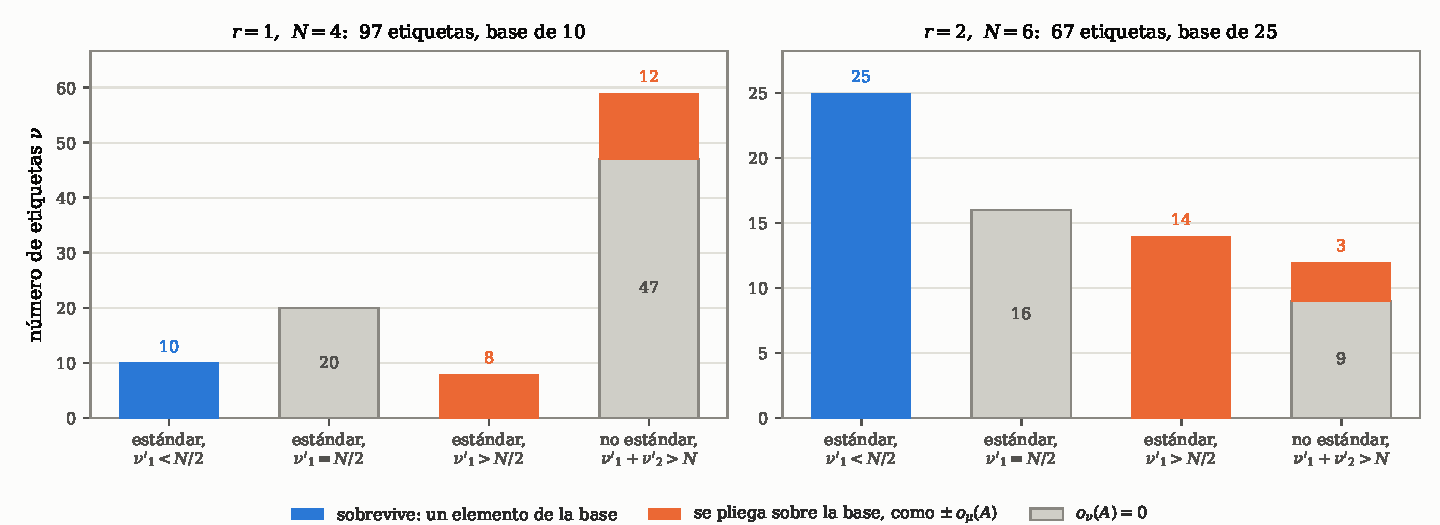
\includegraphics[width=\textwidth]{fig_reduction_es.pdf}
\caption{La reducción del Lema \ref{lem:AtoSp}, dibujada. Cada etiqueta
$\nu$ que aparece en $s_\lambda=\sum_\nu c_\nu o_\nu$ se coloca en una de cuatro clases y se calcula
su valor $o_\nu(A)$. Las etiquetas autoasociadas se anulan, todas ellas; las estándar con
$\nu'_1>N/2$ se pliegan sobre la base como $\pm o_{\mu}(A)$; las no estándar o se anulan o se pliegan
sobre un único elemento de la base con coeficiente $\pm1$. Por \eqref{eq:AtoSp} estas tres son las
reglas de modificación simplécticas disfrazadas, con las clases cortadas por $\ell(\nu)$ frente al
rango $r$; la figura se calculó antes de advertirlo y se deja tal cual. Todo aterriza en la base
independiente $\{o_\mu(A):\ell(\mu)\le r\}$, que es lo que convierte la anulación en la condición
finita \eqref{eq:Cmu}. Las alturas de las barras son recuentos de etiquetas sobre el rango en que se
calculó cada panel, menor que el de la fila correspondiente de la \S\ref{sec:verif}; lo que la imagen
cuenta es la clasificación, no el recuento.}
\label{fig:reduction}
\end{figure}
\begin{equation}\label{eq:Cmu}
\Psi_r(\lambda)=\sum_{\ell(\mu)\le r}C_\mu(\lambda)\,o_\mu(A),
\qquad
\Psi_r(\lambda)=0\iff C_\mu(\lambda)=0\ \text{para toda }\mu,
\end{equation}
donde $C_\mu=c_\mu\pm c_{\mu^{*}}+\sum\pm c_\nu$, sumando sobre las $\nu$ no estándar que se reducen
a $\mu$. La reducción se hace en dos pasos y no en uno: la mayoría de las etiquetas no estándar se
emparejan con una asociada dentro del rango, mientras que $21$ de ellas --- $18$ con $r=1$ y $3$ con
$r=2$ --- no tienen asociada en rango y se reducen aparte, cayendo cada una en el span de los valores
estándar con coeficientes enteros.

Habíamos calculado los tres hechos antes de localizarlos, y dejamos constancia del cálculo porque es
lo que dibuja la figura de abajo: \texttt{sec8\_derivation.sage} comprueba \eqref{eq:AtoSp}
directamente para todo $|\nu|\le8$, confirma que las etiquetas de longitud $r+1$ se anulan y que las
más largas se pliegan sobre la base con un signo, y verifica la independencia como un cálculo de
rango, con $r=1,2,3$. Un control que tenía que dispararse: $\iota_1 o_\nu$ y $\iota_{-1}o_\nu$
coinciden con $sp_\nu$ sólo para $\nu=\varnothing$, de modo que hacen falta las dos letras y
\eqref{eq:AtoSp} es un enunciado sobre el par recíproco y no sobre ninguna de las dos por separado.
\texttt{sec8\_formulas.sage} comprueba la demostración y no el enunciado --- la recurrencia con cuatro
valores de $c$, los dos determinantes que definen los caracteres frente a una implementación
independiente, y las operaciones de columna entrada por entrada. Esta última comprobación se ganó el
sueldo: un borrador previo de la demostración escribía $C_j\to C_j+C_{j-1}$ con $c=1$, que es el signo
que \cite[Lema 3.2]{AK25} usa para su propio paso con $c=-1$.

Las etiquetas no estándar, que son aquí toda la obstrucción, no pueden ser pequeñas:

\begin{lemma}[las etiquetas no estándar son grandes]\label{lem:nonstd}
Toda $\nu$ no estándar que aparezca en el desarrollo cumple $|\nu|\ge N+1=2r+3$. En consecuencia, si
$|\lambda|\le2r+2$ ninguna etiqueta no estándar está contenida en $\lambda$, la última suma de $C_\mu$
queda vacía y $C_\mu(\lambda)=c_\mu(\lambda)\pm c_{\mu^{*}}(\lambda)$ --- sin hipótesis alguna sobre
$\ell(\lambda)$, luego también fuera del rango de Littlewood.
\end{lemma}

\begin{proof}
Como $c^{\lambda}_{\nu\beta'}=0$ salvo si $\nu\subseteq\lambda$, solo aparecen etiquetas con
$\ell(\nu)\le\ell(\lambda)\le N$. Ser no estándar significa $\nu'_1+\nu'_2>N$. Si $\nu$ tuviera una
sola columna sería $\nu'_2=0$ y haría falta $\nu'_1=\ell(\nu)>N$, que queda excluido; luego
$\nu'_2\ge1$ y $|\nu|\ge\nu'_1+\nu'_2>N=2r+2$. Así que una $\nu$ no estándar solo puede contribuir
cuando $|\lambda|\ge|\nu|\ge2r+3$.
\end{proof}

\noindent Como $\ell(\lambda)>N/2$ obliga a $|\lambda|\ge r+2$, el Lema \ref{lem:nonstd} resuelve de
golpe la franja $r+2\le|\lambda|\le2r+2$ del rango inestable: ahí la regla de Littlewood se aplica
literalmente y el recíproco se sigue por el argumento del Teorema \ref{thm:stable}. Lo que esta ruta
todavía tiene que cruzar es $|\lambda|>2r+2$.


Dos hechos exactos acotan a los competidores. Primero, $\ell(\mu^{*})=N-\ell(\mu)$, de modo que
$\ell(\mu)\le N-1-\ell(\lambda)$ obliga a $\mu^{*}\not\subseteq\lambda$ y a $c_{\mu^{*}}=0$. Segundo,
una $\nu$ no estándar cumple $\nu'_1+\nu'_2>N$ con $\nu'_2\le\nu'_1$, luego $2\ell(\nu)>N$ y
$\ell(\nu)\ge r+2$; en particular, en el rango de Littlewood ninguna etiqueta no estándar cabe dentro
de $\lambda$. Llamemos $\mu$ \emph{aislante} para $\lambda$ si exactamente una de las etiquetas que
alimentan $C_\mu$ está contenida en $\lambda$; entonces $C_\mu=\pm c_\nu\ne0$ y
$\Psi_r(\lambda)\ne0$. Lo que la ruta pide ahí es un único enunciado de existencia ---abierto como
enunciado de existencia, aunque no como teorema, pues el Teorema \ref{conj:crit} no pasa por él---.

\begin{proposition}[el testigo aislante no siempre existe]\label{conj:iso}
En $r=2$ la forma $\lambda=(5,5,2,1)$ cumple $\Psi_2(\lambda)\ne0$ y no es de tipo {\rm(a)} ni de
tipo {\rm(b)}, y ninguna $\mu$ es aislante para ella: toda $\mu$ cuyo $C_\mu$ tenga un contribuyente
no nulo dentro de $\lambda$ tiene exactamente dos, a saber $\mu$ y su asociado $\mu^{*}$.
\end{proposition}

Habíamos propuesto el testigo aislante como la vía hacia el Teorema \ref{conj:crit}, y no llega. La
razón se lee en el lema de aislamiento: exige $\ell(\mu)\le N-1-\ell(\lambda)$, lo que con
$\ell(\lambda)=4$ y $N=6$ deja solo $\mu$ de una fila, y una forma tan ancha como $(5,5,2,1)$
contiene a todos los asociados. Sobre $r=2$ y $|\lambda|\le14$ hay once formas así, la menor esta
misma, y ninguna por debajo de $|\lambda|=13$, que es la razón de que el certificado parezca sólido
en rangos pequeños. El Teorema \ref{conj:crit} en sí queda intacto ---afirma que los $C_\mu$ se
anulan, no que exista un certificado--- pero esta vía hacia él queda cerrada. La que sí llega, la
\S\ref{sec:rigidity}, no pasa por el rango de Littlewood, y por eso el fallo de aquí cuesta la
explicación y no el teorema.

El mecanismo alcanza mucho: en $r=2$ y $|\lambda|\le14$, $227$ de las $238$ formas inestables no
nulas llevan un testigo aislante demostrado. Y alcanza más de lo que el hecho (ii) permite por sí
solo ---el mínimo real de $\ell(\nu)$ sobre las $\nu$ no estándar con $o_\nu(A)\ne0$ es allí $5$,
frente al $r+2=4$ que da la cota. Lo que lo derrota es la anchura y no la altura: la base de
\eqref{eq:Cmu} crece con $r$ y las etiquetas competidoras están obligadas a ser altas, así que
leíamos el aislamiento como algo que se facilita con $r$, y a lo largo del eje de la altura así es;
el residuo vive donde $\lambda$ es lo bastante ancha para tragarse los asociados. Esa lectura predice
dónde el residuo \emph{no} está: en $r=3$ el lema de aislamiento permite $\ell(\mu)\le7-\ell(\lambda)$,
de modo que una forma tiene que ser más ancha que en $r=2$ antes de poder tragarse todos los
asociados, y los mismos tamaños deberían salir limpios. Y salen ---sobre $r=3$ y $|\lambda|\le13$ las
$149$ formas inestables no nulas llevan todas un testigo demostrado y el residuo es vacío---, lo cual
es un control sobre la explicación, no un paso hacia el Teorema \ref{conj:crit}. En $r=1$ la
cuestión no se plantea, pues ese caso lo resuelve por separado el Teorema \ref{thm:r1}.

La herramienta a la que uno acude primero no encaja. La saturación, en la forma de panal de Knutson
y Tao \cite{KT99}, decide cuándo un coeficiente de Littlewood--Richardson aislado es positivo, y todo
competidor que alimenta a $C_\mu$ lo es en cuanto su etiqueta cabe dentro de $\lambda$. Lo que un
$\mu$ aislante pide no es positividad sino \emph{aislamiento}: que exactamente uno de ellos quepa. La
positividad es lo que vuelve difícil la pregunta, no lo que la responde, y no conocemos herramienta
alguna dirigida a la segunda.

\begin{figure}[t]
\centering
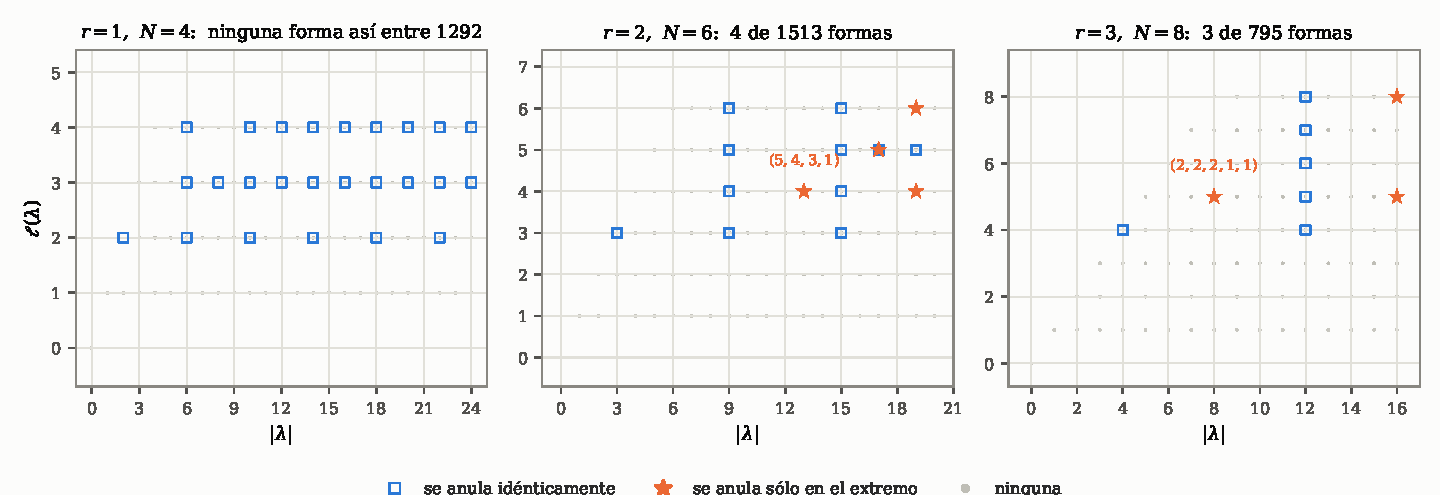
\includegraphics[width=\textwidth]{fig_phase_es.pdf}
\caption{Dónde deja de ser típico un solo par recíproco. Cada partición con a lo sumo $N$ partes es un
punto en $(|\lambda|,\ell(\lambda))$; la clase dibujada con estrella es la que se anula en el extremo
$z_i=1$ sin anularse idénticamente, y es todo el contenido de la imagen; cada panel nombra a su
miembro más pequeño y la Observación \ref{rem:rankone} enumera los demás.
Los paneles cubren $|\lambda|\le24$, $20$ y $16$ respectivamente. En $r=1$ la clase
está vacía sobre las $1292$ formas del rango, porque allí el objeto es $\pm$ un carácter genuino y su
valor en la identidad es una dimensión. A partir de $r=2$ aparecen ejemplos genuinamente virtuales y
la clase deja de estar vacía ---no que toda forma lo sea: el Cuadro \ref{tab:virtual} cuenta las dos
cosas---. Véase la Observación \ref{rem:rankone}.}
\label{fig:phase}
\end{figure}

\begin{remark}[el accidente de rango uno, y dónde se separan los dos rangos]\label{rem:rankone}
En $r=1$ el objeto es $\pm$ un carácter genuino, así que su valor en la identidad es una dimensión y
$\Psi_1(\lambda)\equiv0$ si y solo si $\Psi_1(\lambda)|_{z=1}=0$. En $r\ge2$ la expansión plegada
\emph{puede} ser genuinamente virtual ---no que lo sea siempre, y el Cuadro \ref{tab:virtual} cuenta
las dos columnas---, y basta una forma en que lo sea para romper esa equivalencia:
$\lambda=(5,4,3,1)$ con $r=2$ cumple
$\Psi_2(\lambda)\ne0$ y $\Psi_2(\lambda)|_{z_1=z_2=1}=0$. La Figura \ref{fig:virtual} muestra
los dos regímenes uno al lado del otro, sobre dos formas que difieren en una sola casilla. Sobre los rangos de la Figura
\ref{fig:phase}, la clase de tales formas está vacía en $r=1$ a lo largo de $1292$ particiones; en
$r=2$ consta de las cuatro formas $(5,4,3,1)$, $(5,5,4,2,1)$, $(10,5,3,1)$ y $(6,5,4,2,1,1)$, y en
$r=3$ de las tres formas $(2,2,2,1,1)$, $(5,5,4,1,1)$ y $(3,3,3,2,2,1,1,1)$; es delgada, pero no está
vacía, y un solo contraejemplo es todo lo que la equivalencia puede soportar. La implicación que sí
sobrevive ---anulación exacta $\Rightarrow$ anulación en el extremo--- es lo que hace del extremo un
tamiz válido y nada más. Por eso los resultados calculados en elementos de orden dos ---Karmakar
\cite{Kar24} a lo largo de toda esa familia, Eisenkölbl \cite{Eis07} en el equilibrado
$x_i=(-1)^i$--- hablan de un punto y no de la curva, y por eso el
Teorema \ref{thm:zeros} no es un corolario suyo para $r\ge2$.
\end{remark}

Conviene ponerle un número a lo que el tamiz del extremo deja escapar, porque el enunciado
cualitativo se lee con facilidad como una corrección pequeña. Sobre los rangos de la Figura
\ref{fig:phase}, el contraste $\Psi_r(\lambda)|_{z_i=1}=0$ señala $143$ formas en $r=1$, $22$ en $r=2$
y $9$ en $r=3$; de ellas, $0$, $4$ y $3$ respectivamente no se anulan idénticamente. El tamiz es
entonces exacto con un solo par, y la proporción de sus veredictos que resultan espurios crece con el
número de pares: $0\%$, $18\%$, $33\%$ sobre estos rangos. Un cálculo en el extremo es un filtro que
nunca se salta un cero genuino, y pasado un par no es nada más que eso. El caso de rango uno con
$t=2$, donde el tamiz resulta exacto porque el objeto es un carácter genuino, se trató aparte en
\cite{Mar26}; el alfabeto \eqref{eq:object} surgió allí, en un cálculo de líneas de Wilson sobre un
orbifold, y de ahí que el $-1$ aparezca como letra y no como elección.

Vale la pena separar la razón de que los dos rangos de $\ell(\lambda)$ se comporten de forma tan
distinta del mecanismo que lo demuestra. La regla de Littlewood dice qué etiquetas $\nu$ pueden
aparecer, y $\ell(\lambda)\le N/2$ es exactamente la condición bajo la cual las no estándar no caben
dentro de $\lambda$. El Lema \ref{lem:nonstd} dice que la obstrucción la gobierna $|\lambda|$ además
de $\ell(\lambda)$, así que la imagen honesta no es de dos rangos sino de una región: \emph{esta
ruta} alcanza el recíproco allí donde $\ell(\lambda)\le N/2$ o bien $|\lambda|\le2r+2$, y fuera de la
unión de ambas no llega ---el testigo aislante cubre casi todo lo que queda pero demostrablemente no
todo, por la Proposición \ref{conj:iso}---. El recíproco no está abierto ahí. El Teorema
\ref{conj:crit} lo resuelve para todo $r$ y toda $\lambda$ por el argumento extremal de las
\S\S\ref{sec:extremal}--\ref{sec:rigidity}, que no entra en este rango en absoluto. Lo que la región
marca es dónde deja de explicar la reducción de Littlewood, no dónde deja de valer el teorema.

%======================================================================
% ---- v2_new_subsections_es.tex ----
\subsection{El criterio en \texorpdfstring{$t=2$}{t=2}: el argumento extremal}\label{sec:extremal}

En esta subsección y en las dos siguientes, $t\ge2$ y $r\ge1$ son arbitrarios y
\[
  N:=t+2r,\qquad
  \Phi_{t,r}(\lambda;z):=s_\lambda\bigl(\zt,\,z_1,\zb_1,\dots,z_r,\zb_r\bigr),
\]
de modo que $\Phi_{t,1}$ es \eqref{eq:object} y $\Phi_{2,r}=\Psi_r$. El beta-conjunto, los recuentos
de residuos $n_i$ y la indexación de las columnas son los de la \S\ref{sec:background}; $\lambda\in\PP_N$ y
$\beta_1>\dots>\beta_N\ge0$. Escribimos
\[
  \mathcal{E}=\{i:n_i(\lambda)\ge2\},\qquad e=|\mathcal{E}|,\qquad
  \mathcal{S}=\{\beta_j:\beta_j\equiv i\ (t)\ \text{para algún } i\in\mathcal{E}\}
\]
para las \emph{clases de exceso} y los \emph{valores de exceso}. Como las $t-e$ clases restantes son
unitarias, \eqref{eq:excess} se convierte en
\begin{equation}\label{eq:excessgen}
  \sum_{i\in\mathcal{E}}\bigl(n_i(\lambda)-1\bigr)=2r,\qquad |\mathcal{S}|=2r+e,\qquad 1\le e\le2r .
\end{equation}
Suponemos siempre la \emph{hipótesis de ocupación} $n_i\ge1$ para todo $i$; por el Lema
\ref{lem:L1} su fallo da $\Phi_{t,r}\equiv0$ de entrada, que es la rama (a).

\begin{lemma}[la descomposición de Laplace, $r$ general]\label{lem:L3gen}
Sea $\mathcal T$ el conjunto de los $t$-subconjuntos $S$ de columnas que llevan los $t$ residuos, y
para $S\in\mathcal T$ sea $A(S^{c})$ el menor de $\det(x_i^{\beta_j})$ sobre las $2r$ filas que
llevan $z_1,\zb_1,\dots,z_r,\zb_r$ y las columnas $S^{c}$. Entonces
\begin{equation}\label{eq:laplacegen}
  \det\bigl(x_i^{\beta_j}\bigr)_{i,j=1}^{N}
  \;=\;(-1)^{\binom{t+1}{2}}\,V\sum_{S\in\mathcal T}w(S)\,A(S^{c}),
  \qquad
  w(S)=(-1)^{\,\sum_{j\in S}j+\inv(b_S)} .
\end{equation}
\end{lemma}

\begin{proof}
Laplace por las $t$ primeras filas da
\[
\det(x_i^{\beta_j})=\sum_{|S|=t}(-1)^{\binom{t+1}{2}+\sum_{j\in S}j}M_S\,A(S^{c}).
\]
Por el Lema
\ref{lem:L1}, $M_S=0$ salvo que los residuos $b_S$ sean distintos dos a dos --- es decir, salvo que
$S\in\mathcal T$ --- y entonces $M_S=(-1)^{\inv(b_S)}V$.
\end{proof}

En $r=1$ el menor complementario es el determinante $2\times2$ igual a $f(\beta_{j_1}-\beta_{j_2})$ y
\eqref{eq:laplacegen} es el Lema \ref{lem:L3}; lo que sigue es lo que sustituye a ese menor
$2\times2$ cuando $r>1$. Sólo importan los signos relativos $w(S)$ y, como un elemento de
$\mathcal T$ queda determinado por qué valor de exceso conserva en cada clase de exceso --- las
clases unitarias las conserva todo $S$ ---, indexamos los términos por esa elección, escrita $g$, y
ponemos $T_g=\mathcal{S}\setminus g$, un conjunto de $2r$ valores escritos en orden decreciente.

Conviene resolver aquí una pregunta, porque todo lo que sigue mueve $g$ de un lado a otro y hay que
llevarse el signo consigo: qué le pasa a $w$ cuando cambia la elección en una sola clase. En $r=1$
eso es el Lema \ref{lem:L4}, donde una clase tiene dos elementos y no hay nada entre medias. En
general sí lo hay.

\begin{lemma}[el movimiento de columna, con clases de cualquier tamaño]\label{lem:step}
Sean $g$ y $g'$ coincidentes fuera de una clase, y elijan en ella los valores $u>v$ respectivamente.
Entonces
\begin{equation}\label{eq:step}
\frac{w(g')}{w(g)}\;=\;(-1)^{\,1+B+M},
\end{equation}
donde $B=\#\{\beta_j:v<\beta_j<u\}$ y $M$ es el número de valores \emph{congelados} que quedan
estrictamente entre $v$ y $u$ ---los $t$ valores que una transversal conserva, uno en cada clase de
residuos, o sea los $e$ valores de $g$ junto con las $t-e$ clases singleton---. Puede contarse en $g$
o en $g'$ indistintamente, pues coinciden estrictamente entre $v$ y $u$.
\end{lemma}

\begin{proof}
Los dos conjuntos congelados difieren en sustituir la columna de $u$ por la de $v$. Como $\beta$ es
estrictamente decreciente, ese índice de columna aumenta en $B+1$, que es la variación de
$\sum_{j\in S}j$. En la palabra $b_S$ la letra que lleva esa columna se desplaza por delante de
exactamente las $M$ letras congeladas que quedan estrictamente en medio, y cada cruce cambia $\inv$
en uno; la letra en sí no cambia, y las $B-M$ columnas intermedias que \emph{no} están congeladas no
aportan ninguna letra. Así que $\inv(b_S)$ varía en $M$ módulo $2$, y \eqref{eq:step} se sigue de la
definición de $w$ en el Lema \ref{lem:L3gen}.
\end{proof}

\noindent El Lema \ref{lem:L4} es el caso $B=M=0$ de éste, leído dos veces. La contabilidad es la
misma que Albion \cite{Alb23,Alb25} y Ayyer--Behrend \cite{AB19} hacen cada vez que mueven o invierten
un bloque de columnas y recogen el signo, y la seguimos porque es la que este tipo de determinante
pide; la escribimos en esta forma sólo porque la \S\ref{sec:rigidity} mueve una columna muchas veces
y la cuenta tiene entonces que ser exacta y no absorbida en una constante. Los dos términos tienen
que estar los dos: quitar cualquiera de ellos da una regla que acierta aproximadamente la mitad de
las veces, y $B-M$ es exactamente el número de columnas intermedias que ninguna transversal congela
---por lo cual una clase de tamaño dos, sin nada entre sus elementos, esconde la distinción---. Las
clases singleton hay que contarlas también en $M$, y no es una formalidad: leer $M$ sólo sobre las
elecciones $g$ ya falla en $t=3$, $r=1$ con $\beta=(4,3,2,1,0)$, donde mover la clase del $1$ de
$u=4$ a $v=1$ da $B=2$ y un valor congelado intermedio que vive en una clase singleton, de modo que
las dos lecturas difieren en un signo.

\subsubsection*{La filtración por grados}

Para un monomio $\prod_j z_j^{c_j}$ usamos el \emph{grado total} $\sum_j c_j$. Todo monomio de
$A(S^{c})$ tiene la forma $\prod_j z_j^{\,u-u'}$ para un emparejamiento de $T_g$ en pares ordenados
asignados a las variables, así que, escribiendo $T=(u_1>\dots>u_{2r})$,
\begin{equation}\label{eq:deggen}
  \deg(T):=\sum_{a\le r}u_a-\sum_{a>r}u_a
\end{equation}
es el mayor grado total que aparece en $A$, alcanzado exactamente por los emparejamientos que unen la
mitad de arriba $H=(u_1,\dots,u_r)$ con la de abajo $L=(u_{r+1},\dots,u_{2r})$. Escribiendo
$a_X(z)=\det(z_j^{X_i})_{r\times r}$ y $P(T)=a_H(z)a_L(z^{-1})$, que no es nulo por ser producto de
dos alternantes de $GL(r)$, la componente de grado total máximo de $A$ es
\begin{equation}\label{eq:Amaxgen}
  [A]_{\deg(T)}\;=\;(-1)^{\binom r2}\,P(T).
\end{equation}
En efecto, en grado máximo cada variable recibe una fila de $H$ con exponente positivo y una de $L$
con exponente negativo, y las dos asignaciones son independientes, así que la suma se factoriza en
los dos determinantes; el signo es el de la permutación que reparte las filas de $H$ entre las
columnas $z_1,\dots,z_r$ y las de $L$ entre las columnas $z_1^{-1},\dots,z_r^{-1}$, intercalándolas,
y vale $(-1)^{\binom r2}$.
Bajo la graduación por $\sum_j|c_j|$ la componente máxima se parte en $2^r$ sectores de orientación
con monomios disjuntos, permutados por $z_j\mapsto z_j^{-1}$ con un signo uniforme, así que se anulan
a la vez; todos los enunciados de abajo usan el grado total.

\begin{lemma}[reflexión]\label{lem:reflgen}
$P(c-T)=P(T)$ para todo $c\in\ZZ$ y todo $T$.
\end{lemma}

\begin{proof}
La mitad de arriba de $c-T$ es $c-L$ listada en orden decreciente, así que
$a_{c-L}(z)=(\prod_j z_j^{c})(-1)^{\binom r2}a_L(z^{-1})$, y simétricamente para la mitad de abajo.
Las dos potencias de $\prod_j z_j^{c}$ se cancelan y $(-1)^{r(r-1)}=+1$.
\end{proof}

Sea $G$ el conjunto de las $g$ que maximizan $\deg(T_g)$ y $D_1$ ese máximo. Como el numerador
$\det(x_i^{\beta_j})$ y $\Phi_{t,r}$ difieren en el factor no nulo $\det(x_i^{N-j})$, se tiene
$\Phi_{t,r}\equiv0$ si y sólo si el numerador se anula, y \emph{todo grado y todo estrato de aquí en
adelante se refieren al numerador}; no se compara ninguna de sus partes homogéneas con las del
cociente. Por \eqref{eq:laplacegen},
\begin{equation}\label{eq:topgen}
  \bigl[\det(x_i^{\beta_j})\bigr]_{D_1}
  =(-1)^{\binom{t+1}{2}+\binom r2}\,V\sum_{g\in G}w(g)\,P(T_g),
\end{equation}
donde el segundo signo viene de \eqref{eq:Amaxgen}. Abajo sólo importan los signos relativos $w(g)$,
así que la constante global se anota una vez y no se arrastra.

\begin{remark}[un aviso sobre ese signo global]
Es tentador suprimir $(-1)^{\binom r2}$ con el argumento de que nada de lo que sigue depende de él, y
lo anotamos por la razón contraria: una identidad enunciada es una identidad que se comprueba, y ésta
es \emph{falsa} sin él en cuanto $r\ge2$. El signo no es adorno. Es la signatura de la permutación
intercalada de \eqref{eq:Amaxgen} --- $+1$ para $r=1$ y para $r\equiv0,1 \pmod 4$, $-1$ en los demás
casos --- y es
invisible en $r=1$, que es justo el rango en el que uno escribe la fórmula por primera vez.
\end{remark}

% ---- v2_block2_es.tex ----
\subsubsection*{El conjunto extremal tiene a lo sumo dos elementos}

Para $i\in\mathcal{E}$ listamos los valores de exceso de la clase en orden decreciente,
$c_{i,1}>c_{i,2}>\dots>c_{i,n_i}$ con $n_i=n_i(\lambda)$, y definimos sus \emph{incrementos}
\begin{equation}\label{eq:incrgen}
  \Delta_i(k)\;:=\;c_{i,k}+c_{i,k+1},\qquad 1\le k\le n_i-1 .
\end{equation}
Por \eqref{eq:excessgen} hay exactamente $2r$ en total; escribimos
$\Delta_{(1)}\ge\dots\ge\Delta_{(2r)}$ para la lista en orden decreciente y ponemos
$\tau:=\Delta_{(r)}$.

\begin{theorem}[el conjunto extremal]\label{thm:Ggen}
Supóngase $n_i\ge1$ para todo $i$. Entonces
\begin{enumerate}
\item[\rm(a)] $g\in G$ si y sólo si el multiconjunto de incrementos que selecciona, en el sentido del
Paso 2 de abajo, consta de todos los incrementos $>\tau$ junto con suficientes incrementos iguales a
$\tau$;
\item[\rm(b)] $|G|\le2$, y $|G|=2$ si y sólo si $\Delta_{(r)}=\Delta_{(r+1)}$, en cuyo caso $t$ es
par, los dos incrementos empatados pertenecen a las clases $i$ e $i+t/2$ --- ambas necesariamente en
$\mathcal{E}$ --- y los dos maximizadores difieren exactamente en esas dos clases;
\item[\rm(c)] si $t$ es impar entonces $|G|=1$.
\end{enumerate}
\end{theorem}

\begin{proof}
\emph{Paso 1 (reformulación).} Para todo $2r$-conjunto $T$,
\[
\deg(T)=\max_{A\subseteq T,\,|A|=r}\bigl(2\Sigma A-\Sigma T\bigr),
\]
con el máximo alcanzado en la mitad de arriba. Con $T=\mathcal{S}\setminus g$ esto se lee
$\deg(\mathcal{S}\setminus g)=\max_A\bigl[2\Sigma A+\Sigma g\bigr]-\Sigma\mathcal{S}$, de modo que
maximizamos $\Theta(A,g)=2\Sigma A+\Sigma g$ sobre pares disjuntos con $|A|=r$ y $g$ una elección de
un valor de exceso en cada clase de exceso.

\emph{Paso 2 (forma de un óptimo).} Sea $(A,g)$ óptimo y sean $x>y$ de la misma clase $i$. Si $y\in A$
y $x=g_i$, intercambiarlos deja $g$ admisible y cambia $\Theta$ en $x-y>0$; si $y=g_i$ y $x$ no está
ni en $A$ ni en $g$, el mismo intercambio da $x-y>0$. Ambos son imposibles, así que dentro de cada
clase, leída en orden decreciente, van primero los elementos de $A$, luego $g_i$, y luego los no
elegidos. Por tanto un óptimo queda parametrizado por un entero por clase,
$k_i=|A\cap\text{clase }i|\in\{0,\dots,n_i-1\}$ con $\sum_i k_i=r$, mediante
$A\cap\text{clase }i=\{c_{i,1},\dots,c_{i,k_i}\}$ y $g_i=c_{i,k_i+1}$. La aplicación $(k_i)\mapsto g$
es inyectiva y, fijado $g$, el $A$ óptimo es la mitad de arriba de $T_g$, así que los pares óptimos se
proyectan biyectivamente sobre $G$.

\emph{Paso 3 (separabilidad).} Con esa parametrización $\Theta=\sum_{i\in\mathcal{E}}f_i(k_i)$, con
$f_i(k)=2(c_{i,1}+\dots+c_{i,k})+c_{i,k+1}$: el objetivo se parte sobre las clases y el único
acoplamiento es $\sum_i k_i=r$.

\emph{Paso 4 (el intercambio).} $f_i(k)-f_i(k-1)=\Delta_i(k)$, estrictamente decreciente en $k$
porque los $c_{i,k}$ lo son, luego
\[
\Theta=\sum_{i\in\mathcal{E}}f_i(0)+\Sigma,\qquad
\Sigma=\sum_{i\in\mathcal{E}}\sum_{k\le k_i}\Delta_i(k),
\]
y maximizar $\Theta$ es maximizar $\Sigma$. Un $(k_i)$ factible selecciona, en cada clase, un
\emph{prefijo} de la lista de incrementos de esa clase, con $r$ incrementos en total; llamemos
\emph{admisible} a una selección así. Tómese ahora cualquier conjunto de $r$ incrementos de suma
máxima, sea admisible o no. Esa selección \emph{es} admisible: si contuviera $\Delta_i(k)$ sin
$\Delta_i(k-1)$, intercambiar los dos subiría la suma, porque $\Delta_i(k-1)>\Delta_i(k)$ ---y el
intercambio es legítimo porque $\Delta_i(k-1)$ no estaba ya seleccionado---. Y ninguna selección
admisible puede superar la suma de los $r$ incrementos mayores, siendo ella misma una selección de
$r$ de ellos. Luego los maximizadores de $\Theta$ son exactamente las selecciones admisibles cuyo
multiconjunto de incrementos es un multiconjunto de $r$ mayores, que es lo que afirma {\rm(a)}.
(Es el algoritmo voraz de asignación marginal para un objetivo separable cóncavo bajo una
restricción de cardinal; véanse \cite{FG86,IK88}. Damos el argumento porque son cuatro líneas, de
modo que el Teorema \ref{conj:crit} no se apoye en más resultado ajeno que el Teorema
\ref{thm:PvW}.)

\emph{Paso 5 (residuos).} $c_{i,k}\equiv c_{i,k+1}\equiv i$, luego
\begin{equation}\label{eq:congrgen}
  \Delta_i(k)\;\equiv\;2i \pmod t .
\end{equation}
Dentro de una clase los incrementos son distintos dos a dos por el Paso 4. Entre clases,
$\Delta_i(k)=\Delta_{i'}(k')$ fuerza $2i\equiv2i'$, es decir $i'=i$ o --- sólo si $t$ es par ---
$i'=i+t/2$. Por tanto \emph{ningún valor lo comparten más de dos incrementos}, y cuando lo comparten,
los dos vienen de las clases $i$ e $i+t/2$.

\emph{Paso 6.} Los óptimos son las selecciones que contienen todo incremento $>\tau$ junto con $s$ de
los iguales a $\tau$, con $s\ge1$. A lo sumo dos incrementos valen $\tau$, así que o caben los dos
($|G|=1$) o cabe exactamente uno ($|G|=2$), esto último precisamente cuando
$\Delta_{(r)}=\Delta_{(r+1)}$. Para $t$ impar, $x\mapsto2x$ es inyectiva en $\ZZ/t$, así que no hay
empate posible y $|G|=1$.
\end{proof}

\begin{remark}
El contenido del Teorema \ref{thm:Ggen} es \eqref{eq:congrgen} junto con el hecho de que
$x\mapsto2x$ en $\ZZ/t$ tiene núcleo de orden $\gcd(2,t)$: la multiplicidad de un valor extremal la
controla la $2$-torsión del grupo de residuos, que es la razón de que la paridad de $t$ lo gobierne
todo aquí y en la \S\ref{sec:main}. Los Pasos 1--4 sólo usan que los $\beta_j$ sean enteros
distintos; ni $\beta_j\ge0$, ni que $\lambda$ sea una partición, ni $N=t+2r$ intervienen más allá de
\eqref{eq:excessgen}. La Figura \ref{fig:increments} es el teorema hecho sobre una forma concreta,
con el empate y la forma de prefijo del Paso 2 a la vista.
\end{remark}

\begin{remark}[de dónde viene esta forma de argumento]
Los Pasos 1--4 son una historia vieja contada en otro alfabeto. Maximizar un objetivo separable
cóncavo bajo una restricción de cardinal es el problema clásico de asignación marginal de recursos,
que resuelve el algoritmo voraz \cite{FG86,IK88}; hemos dado el intercambio en cuatro líneas sólo para
que el lector no tenga que salir del artículo. El Paso 6 también es conocido, aunque venga de otra
tradición: en álgebra lineal tropical la forma inicial de un determinante es la suma con signo sobre
las asignaciones \emph{óptimas}, y la matriz se llama tropicalmente singular exactamente cuando dos o
más óptimos alcanzan el óptimo \cite{TropCramer}. Leída así, \eqref{eq:topgen} dice que nuestro
numerador es tropicalmente singular precisamente cuando $|G|=2$, y toda la cuestión de la
\S\ref{sec:rigidity} es si los dos óptimos se cancelan. Lo que \emph{no} es estándar, y es la razón de
que la paridad de $t$ lo gobierne todo, es \eqref{eq:congrgen}: es una congruencia, no una
desigualdad, y es lo que acota por dos el número de óptimos.
\end{remark}

\begin{figure}[!ht]
\centering
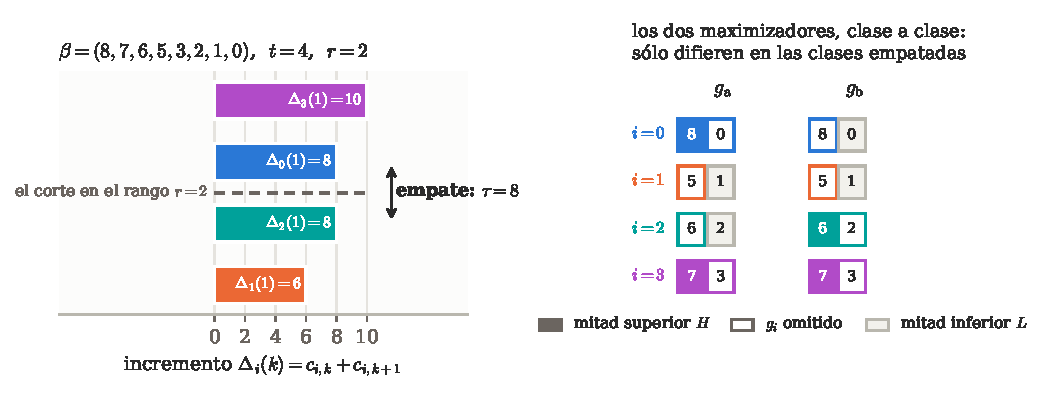
\includegraphics[width=\textwidth]{fig_increments_es.pdf}
\caption{El Teorema \ref{thm:Ggen} hecho sobre una forma, en vez de enunciado. Para
$\beta=(8,7,6,5,3,2,1,0)$ con $t=4$, $r=2$ las cuatro clases de exceso son $\{8,0\}$, $\{5,1\}$,
$\{6,2\}$, $\{7,3\}$ y los cuatro incrementos son $\Delta_3(1)=10$, $\Delta_0(1)=8$,
$\Delta_2(1)=8$, $\Delta_1(1)=6$. Un maximizador toma los $r=2$ mayores; el segundo y el tercero son
iguales, así que $\tau=\Delta_{(2)}=\Delta_{(3)}=8$ y hay exactamente dos. La pareja empatada
pertenece a las clases $0$ y $2=0+t/2$, que es \eqref{eq:congrgen} y no una casualidad: ningún valor
lo comparten incrementos de clases distintas de $i$ e $i+t/2$. A la derecha los dos maximizadores
están dibujados clase a clase en la forma de prefijo del Paso 2 --- leyendo una clase en orden
decreciente, primero los elementos de la mitad de arriba, luego el omitido $g_i$, luego los de la
mitad de abajo ---, lo que hace visible que difieren en las clases empatadas y en ninguna otra. El
color codifica la clase, no el rango. Calculada por \texttt{anc/fig\_v2.py}.}
\label{fig:increments}
\end{figure}

\begin{corollary}[un maximizador único]\label{cor:uniquegen}
Si $|G|=1$ entonces $\Phi_{t,r}\not\equiv0$.
\end{corollary}

\begin{proof}
Por \eqref{eq:topgen} la componente del numerador en grado $D_1$ es $\pm V\,P(T_g)\ne0$ para el único
$g$. Un polinomio de Laurent con una componente homogénea no nula no es nulo, así que el numerador no
es nulo y por tanto tampoco lo es $\Phi_{t,r}$.
\end{proof}

\begin{corollary}[el bloque central]\label{cor:midgen}
Escríbase $\mathcal{S}=\{s_1>\dots>s_n\}$, $n=2r+e$. Si el bloque $\{s_{r+1},\dots,s_{r+e}\}$
contiene exactamente un elemento de cada clase de exceso, entonces $\Phi_{t,r}\not\equiv0$.
\end{corollary}

\begin{proof}
$\deg(\mathcal{S}\setminus g)\le(s_1+\dots+s_r)-(s_{n-r+1}+\dots+s_n)$, porque los $r$ elementos
mayores de $\mathcal{S}\setminus g$ están dominados término a término por $s_1,\dots,s_r$ y sus $r$
menores dominan a $s_{n-r+1},\dots,s_n$. La igualdad obliga a que $\mathcal{S}\setminus g$ contenga
los dos bloques extremos, es decir $g\subseteq\{s_{r+1},\dots,s_{r+e}\}$, y $|g|=e$ fuerza la igualdad
de los dos conjuntos. Así que la cota la alcanza exactamente un término y se aplica el Corolario
\ref{cor:uniquegen}.
\end{proof}

\begin{corollary}[$t$ impar]\label{cor:oddgen}
Sea $t$ impar y $r\ge1$. Entonces $\Phi_{t,r}(\lambda;z)\equiv0$ si y sólo si alguna clase de residuos
módulo $t$ está ausente de $\beta(\lambda)$.
\end{corollary}

\begin{proof}
Si algún $n_i=0$ entonces $\mathcal T=\varnothing$ en el Lema \ref{lem:L3gen} y el numerador se anula.
Recíprocamente, si todos los $n_i\ge1$ entonces $|G|=1$ por el Teorema \ref{thm:Ggen}(c) y se aplica
el Corolario \ref{cor:uniquegen}.
\end{proof}

\begin{remark}
Para $r=1$ el Corolario \ref{cor:oddgen} es la Proposición \ref{rem:lattice}, demostrada allí viendo
que la cláusula concéntrica es vacua para $t$ impar --- un argumento interno al perfil de dos clases
que fuerza un solo par recíproco. Lo nuevo es que el enunciado sobrevive para todo $r\ge1$, y por una
ruta que no menciona el perfil en absoluto: la congruencia \eqref{eq:congrgen}. En $r=0$ es falso,
puesto que la regla de Littlewood da $s_\lambda(\zt)=0$ siempre que el $t$-núcleo es no vacío, $t$
impar incluido; y la observación de que $\prod\zt=+1$ para $t$ impar no lo entrega por sí sola,
porque el alfabeto es un subtoro de dimensión $r$ con las coordenadas restantes congeladas.
\end{remark}

% ---- v2_block3_es.tex ----
\subsection{El criterio en \texorpdfstring{$t=2$}{t=2}: rigidez y reflexión}\label{sec:rigidity}

El Corolario \ref{cor:uniquegen} resuelve toda forma con un maximizador único. Lo que sigue es la
otra mitad: cuando $|G|=2$, los dos términos de \eqref{eq:topgen} sólo pueden cancelarse si las dos
transversales son reflexión una de otra, y esa rigidez la aporta un único resultado ajeno.

\begin{theorem}[Purbhoo--van Willigenburg {\cite[Thm.~2.5]{PvW}}]\label{thm:PvW}
Para particiones con a lo sumo $n$ partes, escribiendo $\lambda^{-}:=\lambda/(\lambda_n)^{n}$,
\[
  s_\lambda(x_1,\dots,x_n)\,s_\mu(x_1,\dots,x_n)=s_\nu(x_1,\dots,x_n)\,s_\rho(x_1,\dots,x_n)
\]
si y sólo si $\lambda_n+\mu_n=\nu_n+\rho_n$ y $\{\lambda^{-},\mu^{-}\}=\{\nu^{-},\rho^{-}\}$ como
multiconjuntos.
\end{theorem}

\begin{remark}
El Teorema 3 de \cite{Rajan} da el enunciado para $n$ factores, pero bajo la hipótesis de que todos
los pesos máximos sean no nulos. El Teorema \ref{thm:PvW} no necesita tal hipótesis, y por eso es el
que usamos aquí: el caso degenerado, un factor trivial, es exactamente lo que produce el Lema
\ref{lem:dictgen} siempre que $\alpha^{*}$ o $\tilde\alpha$ es vacía. Ninguno de los dos enunciados
puede atajarse por factorización única, ya que los polinomios de Schur no son irreducibles:
$s_{(3)}(x,y)=(x+y)(x^2+y^2)$.
\end{remark}

\subsubsection*{El diccionario}

Escríbase $T=(u_1>\dots>u_{2r})$ con mitades $H=(h_1>\dots>h_r)$ y $L=(l_1>\dots>l_r)$, sea
$\delta=(r-1,r-2,\dots,0)$, de modo que $a_\delta(z)=\det(z_j^{\,r-i})$ es el determinante de
Vandermonde en la notación de la \S\ref{sec:extremal}, y póngase
\[
  \alpha=H-\delta,\qquad \tilde\alpha=\alpha-(\alpha_r)^{r},\qquad
  L^{*}=(l_1-l_r>\dots>l_1-l_1),\qquad \alpha^{*}=L^{*}-\delta .
\]

\begin{lemma}[el diccionario]\label{lem:dictgen}
$\alpha^{*}_r=0$ y
\begin{equation}\label{eq:dictgen}
  P(T)\;=\;(-1)^{\binom r2}\Bigl(\textstyle\prod_j z_j\Bigr)^{h_r-l_1}
  a_\delta(z)^2\,s_{\tilde\alpha}(z)\,s_{\alpha^{*}}(z).
\end{equation}
En particular $P$ no cambia bajo $T\mapsto T+m$ ni, por el Lema \ref{lem:reflgen}, bajo
$T\mapsto c-T$.
\end{lemma}

\begin{proof}
$a_H(z)=s_\alpha(z)a_\delta(z)$ es la fórmula bialternante. Para el segundo factor, multiplicar la
columna $j$ de $\det(z_j^{-l_i})$ por $z_j^{l_1}$ da
$(\prod_j z_j^{l_1})a_L(z^{-1})=\det(z_j^{\,l_1-l_i})$, cuyos exponentes de fila crecen con $i$;
invertir las $r$ filas cuesta $(-1)^{\binom r2}$ y produce $a_{L^{*}}(z)=s_{\alpha^{*}}(z)a_\delta(z)$.
Finalmente $s_\alpha=(\prod_j z_j)^{\alpha_r}s_{\tilde\alpha}$ y $\alpha_r=h_r$.
\end{proof}

\begin{proposition}[la órbita de $P$]\label{prop:orbitgen}
Sean $T,\widetilde T$ conjuntos de $2r$ enteros distintos con $P(T)=\pm P(\widetilde T)$. Entonces
$\widetilde T=T+m$ para algún $m\in\ZZ$, o bien $\widetilde T=c-T$ para algún $c\in\ZZ$.
\end{proposition}

\begin{proof}
Dos observaciones primero. El signo es $+$: por \eqref{eq:dictgen} los dos lados son un monomio por
$a_\delta^2$ por un producto de dos polinomios de Schur, que tiene coeficientes no negativos, así que
un signo menos es imposible. Y el monomio hay que reabsorberlo: con $d=h_r-l_1\ge1$, lo que se cumple
porque $T$ es estrictamente decreciente, $(\prod_j z_j)^{d}s_{\tilde\alpha}=s_{\tilde\alpha+(d^{r})}$,
y es ese $d$ el que hace el papel de $\lambda_n+\mu_n$ en el Teorema \ref{thm:PvW}, estando
$\alpha^{*}$ ya normalizada. Cancelando $a_\delta^2$ y aplicando el Teorema \ref{thm:PvW} con $n=r$ a
$(\lambda,\mu)=(\tilde\alpha+(d^{r}),\alpha^{*})$ y al par correspondiente $(\nu,\rho)$ de
$\widetilde T$, el criterio dice que el entero $d$ coincide y que $\{\tilde\alpha,\alpha^{*}\}$
coincide como multiconjunto. Coincidir en el mismo orden dice que $H,\widetilde H$ y $L,\widetilde L$
son trasladados, y la igualdad de los dos enteros $d$ fuerza la misma traslación en las dos mitades,
es decir $\widetilde T=T+m$. Coincidir tras intercambiar dice que $H$ es, salvo traslación, la
inversa de $\widetilde L$ y $L$ la de $\widetilde H$, es decir $\widetilde T=c-T$.
\end{proof}

\subsubsection*{Los dos maximizadores se reflejan}

De aquí al final de la subsección supóngase $|G|=2$ y escríbase
$G=\{g_{\mathrm a},g_{\mathrm b}\}$, $T_{\mathrm a}=\mathcal{S}\setminus g_{\mathrm a}$,
$T_{\mathrm b}=\mathcal{S}\setminus g_{\mathrm b}$, con mitades
$T_{\mathrm a}=H_{\mathrm a}\sqcup L_{\mathrm a}$ y $T_{\mathrm b}=H_{\mathrm b}\sqcup L_{\mathrm b}$,
y
\[
  \mathcal{K}=T_{\mathrm a}\cap T_{\mathrm b}.
\]
Por el Teorema \ref{thm:Ggen}(b) las dos transversales difieren exactamente en las clases empatadas
$i$ e $i'=i+t/2$, digamos
\begin{equation}\label{eq:swapgen}
  g_{\mathrm a}\ni p_1=c_{i,k+1},\ q_1=c_{i',k'},\qquad
  g_{\mathrm b}\ni p_2=c_{i,k},\ q_2=c_{i',k'+1},
\end{equation}
de modo que $p_1+p_2=q_1+q_2=\tau$ por \eqref{eq:incrgen}: el valor del empate es la suma de cada
pareja intercambiada.

\begin{proposition}[la traslación fuerza la reflexión]\label{prop:translgen}
Si $T_{\mathrm b}=T_{\mathrm a}+m$ con $m\ne0$, entonces $T_{\mathrm b}=\tau-T_{\mathrm a}$.
\end{proposition}

\begin{proof}
$|T_{\mathrm a}\cap(T_{\mathrm a}+m)|=|\mathcal{K}|=2r-2$. Póngase una arista $x\to x+m$ cuando $x$ y
$x+m$ estén los dos en $T_{\mathrm a}$; como $m\ne0$, cada vértice tiene a lo sumo una arista
saliente y una entrante, así que el grafo es una unión disjunta de caminos dirigidos. Tiene $2r$
vértices y, por el cardinal anterior, exactamente $2r-2$ aristas, luego exactamente dos componentes.
Así que $T_{\mathrm a}$ es unión de exactamente dos progresiones aritméticas maximales de paso $m$,
digamos $T_{\mathrm a}=\{p,p+m,\dots,p+(u-1)m\}\cup\{q,\dots,q+(v-1)m\}$ con $u+v=2r$. Entonces
$T_{\mathrm a}\setminus T_{\mathrm b}=\{p,q\}$ y $T_{\mathrm b}\setminus T_{\mathrm a}=\{p+um,q+vm\}$.
El empate dice que $x\mapsto\tau-x$ lleva la primera pareja sobre la segunda, y hay dos
emparejamientos. Si $\tau-p=p+um$ y $\tau-q=q+vm$ entonces
$\tau-T_{\mathrm a}=\{p+m,\dots,p+um\}\cup\{q+m,\dots,q+vm\}=T_{\mathrm b}$. Si $\tau-p=q+vm$ y
$\tau-q=p+um$, restando queda $um=vm$, luego $u=v$, y otra vez
$\tau-T_{\mathrm a}=T_{\mathrm b}$.
\end{proof}

\begin{proposition}[el centro es el valor del empate]\label{prop:centregen}
Si $T_{\mathrm b}=c-T_{\mathrm a}$ entonces $c=\tau$.
\end{proposition}

\begin{proof}
$x\mapsto c-x$ es una involución que lleva $T_{\mathrm a}$ a $T_{\mathrm b}$, luego $T_{\mathrm b}$ a
$T_{\mathrm a}$, luego $\mathcal{K}$ a $\mathcal{K}$; por tanto lleva
$T_{\mathrm a}\setminus\mathcal{K}$ sobre $T_{\mathrm b}\setminus\mathcal{K}$. Por \eqref{eq:swapgen}
esos dos conjuntos son $T_{\mathrm a}\setminus\mathcal{K}=\{p_2,q_2\}$ y
$T_{\mathrm b}\setminus\mathcal{K}=\{p_1,q_1\}$, ya que $T_{\mathrm a}$ omite exactamente $p_1,q_1$ y
$T_{\mathrm b}$ omite exactamente $p_2,q_2$. O bien $c-p_2=p_1$, y entonces $c-q_2=q_1$, de donde
$c=p_1+p_2=\tau$; o bien $c-p_2=q_1$ y $c-q_2=p_1$, y sumando queda
$2c=p_1+p_2+q_1+q_2=2\tau$, otra vez $c=\tau$. En el segundo caso además
$c=p_2+q_1\equiv i+i'\equiv2i+t/2$ mientras que $\tau\equiv2i$ por \eqref{eq:congrgen}, así que
$c=\tau$ forzaría $t/2\equiv0\pmod t$, imposible para $t\ge2$: el emparejamiento cruzado no ocurre.
\end{proof}

\begin{corollary}[la reflexión]\label{cor:reflectgen}
Si $\bigl[\det(x_i^{\beta_j})\bigr]_{D_1}=0$ entonces $|G|=2$ y $T_{\mathrm b}=\tau-T_{\mathrm a}$.
En consecuencia $\tau-\mathcal{K}=\mathcal{K}$ y, como $x\mapsto\tau-x$ también fija $\{p_1,p_2\}$ y
$\{q_1,q_2\}$ como conjuntos,
\begin{equation}\label{eq:Ssymgen}
  \tau-\bigl(\mathcal{K}\cup\{p_1,p_2,q_1,q_2\}\bigr)=\mathcal{K}\cup\{p_1,p_2,q_1,q_2\}.
\end{equation}
\end{corollary}

\begin{proof}
$|G|=1$ queda excluido por el Corolario \ref{cor:uniquegen}. Con $|G|=2$, \eqref{eq:topgen} y
$w(g)=\pm1$ dan $P(T_{\mathrm a})=\pm P(T_{\mathrm b})$; se aplica la Proposición
\ref{prop:orbitgen} y luego las Proposiciones \ref{prop:translgen} y \ref{prop:centregen}. La
identidad $\tau-\mathcal{K}=\mathcal{K}$ es la primera línea de la prueba de la Proposición
\ref{prop:centregen}, y $p_1+p_2=q_1+q_2=\tau$ es el empate.
\end{proof}

\begin{remark}[tres constantes fáciles de confundir]
$\tau=\Delta_{(r)}$ es el valor del empate, un dato del algoritmo voraz ajeno a toda simetría; $c$ es
un centro de reflexión, producido por la rigidez y sin nada que ver con los residuos;
$C=\min\mathcal{S}+\max\mathcal{S}$ es un estadístico del beta-conjunto, y es el que usa la condición
\textup{(ii)}. Que $c=\tau$ \textup{(}Proposición \ref{prop:centregen}\textup{)} y que $C=\tau$
\textup{(}Corolario \ref{cor:Ctaugen}\textup{)} son teoremas, no notación, y los dos necesitan la
hipótesis de anulación: escribir $C$ donde corresponde $\tau$ demuestra menos de lo que parece.
Nosotros cometimos ese desliz; de ahí los tres símbolos.
\end{remark}

\subsubsection*{El centro del beta-conjunto}

Los dos maximizadores coinciden fuera de las clases empatadas, así que su parte omitida común
\begin{equation}\label{eq:gcomgen}
  g_{\mathrm{com}}:=g_{\mathrm a}\cap g_{\mathrm b},\qquad
  \mathcal{S}=\mathcal{K}\ \sqcup\ g_{\mathrm{com}}\ \sqcup\ \{p_1,p_2,q_1,q_2\}
\end{equation}
es vacía exactamente cuando $e=2$. Por \eqref{eq:Ssymgen} el conjunto
$\mathcal{S}\setminus g_{\mathrm{com}}$ es estable bajo $x\mapsto\tau-x$, pero $g_{\mathrm{com}}$ no
tiene por qué serlo, así que $\mathcal{S}$ tampoco. Eso es más de lo que hace falta: sólo los dos
\emph{extremos} de $\mathcal{S}$ tienen que evitar $g_{\mathrm{com}}$, y lo hacen. La Figura
\ref{fig:reflection} dibuja tanto la reflexión como la forma que tiene $|G|=2$ sin ella, que es lo
que la proposición siguiente debe excluir.

\begin{figure}[!ht]
\centering
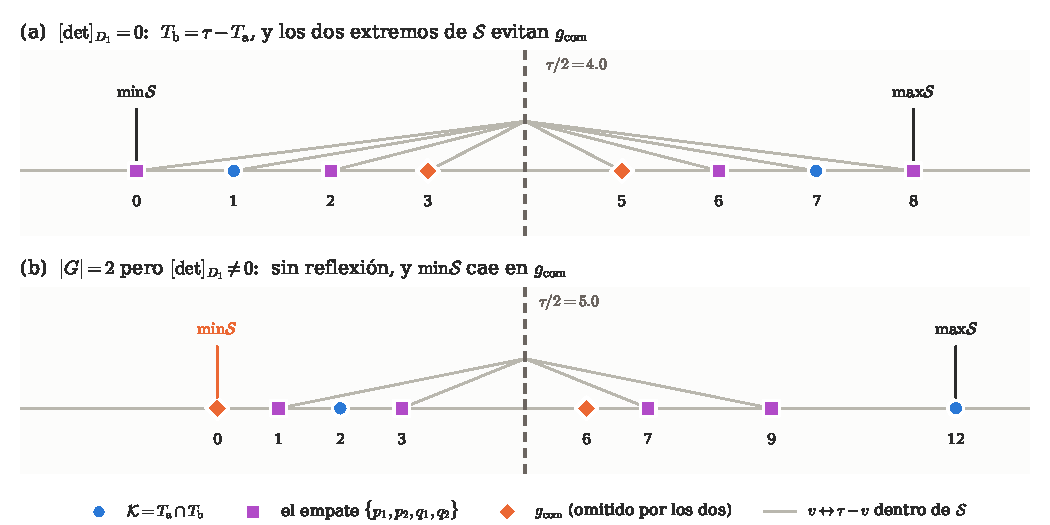
\includegraphics[width=\textwidth]{fig_reflection_es.pdf}
\caption{El Corolario \ref{cor:reflectgen} y la Proposición \ref{prop:A1gen} sobre dos formas, las
dos con $t=4$, $r=2$ y $|G|=2$. Cada panel dibuja $\mathcal{S}$ sobre una recta, coloreada según a
qué parte de \eqref{eq:gcomgen} pertenece el valor; un arco une $v$ con $\tau-v$ cuando los dos están
en $\mathcal{S}$, y la línea discontinua es el centro $\tau/2$. \emph{(a)} $\beta=(8,7,6,5,3,2,1,0)$:
$\tau=8$, $\mathcal{K}=\{1,7\}$, $g_{\mathrm{com}}=\{3,5\}$, empate $\{0,2,6,8\}$. Aquí
$T_{\mathrm b}=\tau-T_{\mathrm a}$, así que $\mathcal{S}\setminus g_{\mathrm{com}}$ es simétrico
respecto de $\tau/2$, y los dos extremos de $\mathcal{S}$ evitan $g_{\mathrm{com}}$, luego
$C=0+8=\tau$. Aquí $g_{\mathrm{com}}=\{3,5\}$ resulta ser simétrico también ---el arco que une sus
dos miembros se dibuja como cualquier otro---, que es lo que la Conjetura \ref{conj:gcom} afirma en
general y lo que la \S\ref{sec:rigidity} no demuestra: la reflexión queda establecida sobre
$\mathcal{S}\setminus g_{\mathrm{com}}$ y observada en el resto.
\emph{(b)} $\beta=(12,9,7,6,3,2,1,0)$: aquí $\tau=10$, y otra vez $|G|=2$, pero los dos maximizadores no
son reflexión uno de otro; $\min\mathcal{S}=0$ cae en $g_{\mathrm{com}}$, y $C=0+12=12\neq\tau$. El
panel (b) es la razón de que la Proposición \ref{prop:A1gen} no pueda demostrarse sólo a partir de
$|G|=2$. Calculada por \texttt{anc/fig\_v2.py}.}
\label{fig:reflection}
\end{figure}


\begin{proposition}[los extremos evitan la parte común]\label{prop:A1gen}
Supóngase $\bigl[\det(x_i^{\beta_j})\bigr]_{D_1}=0$. Entonces
$\max\mathcal{S}\notin g_{\mathrm{com}}$ y $\min\mathcal{S}\notin g_{\mathrm{com}}$.
\end{proposition}

\begin{proof}
Por el Corolario \ref{cor:reflectgen}, $T_{\mathrm b}=\tau-T_{\mathrm a}$. Como $x\mapsto\tau-x$
invierte el orden, lleva la mitad de abajo de $T_{\mathrm a}$ a la de arriba de $T_{\mathrm b}$ y al
revés:
\begin{equation}\label{eq:halvesgen}
  H_{\mathrm b}=\tau-L_{\mathrm a},\qquad L_{\mathrm b}=\tau-H_{\mathrm a}.
\end{equation}
Recuérdese del Paso 2 de la prueba del Teorema \ref{thm:Ggen} que un maximizador queda descrito por
los enteros $k_i$: dentro de la clase $i$, leída en orden decreciente, los primeros $k_i$ valores de
exceso están en la mitad de arriba, el siguiente es el omitido $g_i$, y los restantes están en la
mitad de abajo. Recuérdese también del Teorema \ref{thm:Ggen}(a) que un maximizador selecciona todo
incremento $>\tau$, que los incrementos de una clase se seleccionan en orden de prefijo, y que los
únicos incrementos iguales a $\tau$ son los dos empatados, que viven en las dos clases empatadas.

\emph{El máximo.} Póngase $m=\max\mathcal{S}$ y sea $i$ su clase, de modo que $m=c_{i,1}$ y
$n_i\ge2$; escríbase $c=c_{i,2}$. Entonces $m\in g_{\mathrm a}\cap g_{\mathrm b}$ si y sólo si
$k_i=0$ en los dos maximizadores. Supóngase que sí. Entonces la clase $i$ no está empatada: un
maximizador que toma el incremento empatado de una clase empatada tiene allí $k_i\ge1$. Luego ningún
incremento de la clase $i$ es $\ge\tau$ y, en particular,
\[
  \Delta_i(1)=m+c<\tau .
\]
Por otro lado $k_i=0$ coloca $c$ en la mitad de abajo de los dos maximizadores, así que
$c\in L_{\mathrm b}$, y \eqref{eq:halvesgen} da $\tau-c\in H_{\mathrm a}\subseteq\mathcal{S}$, de
donde $\tau-c\le\max\mathcal{S}=m$, esto es $\tau\le m+c$. Las dos desigualdades mostradas se
contradicen.

\emph{El mínimo} es la imagen especular. Póngase $m^{-}=\min\mathcal{S}$, sea $i^{-}$ su clase,
$n=n_{i^{-}}\ge2$ y $c'=c_{i^{-},n-1}$, de modo que $m^{-}=c_{i^{-},n}$. Entonces
$m^{-}\in g_{\mathrm a}\cap g_{\mathrm b}$ si y sólo si $k_{i^{-}}=n-1$ en los dos, es decir si y
sólo si los dos maximizadores seleccionan \emph{todos} los incrementos de la clase $i^{-}$; otra vez
la clase $i^{-}$ no puede estar empatada, ya que el maximizador que no toma el incremento empatado de
una clase empatada omite allí uno. Luego todo incremento de la clase $i^{-}$ supera a $\tau$, en
particular $\Delta_{i^{-}}(n-1)=m^{-}+c'>\tau$. Y $k_{i^{-}}=n-1$ coloca $c'$ en la mitad de arriba
de los dos, así que $c'\in H_{\mathrm b}$, y \eqref{eq:halvesgen} da
$\tau-c'\in L_{\mathrm a}\subseteq\mathcal{S}$, de donde $\tau-c'\ge\min\mathcal{S}=m^{-}$, esto es
$\tau\ge m^{-}+c'$. Contradicción.
\end{proof}

\begin{corollary}[el centro es el valor del empate]\label{cor:Ctaugen}
Si $\bigl[\det(x_i^{\beta_j})\bigr]_{D_1}=0$ entonces $C:=\min\mathcal{S}+\max\mathcal{S}=\tau$, y
$\mathcal{S}$ corta a todas las clases de residuos de las dos empatadas. Además $t$ es par y las dos
clases empatadas son exactamente las dos soluciones de $2\kappa\equiv C\pmod t$, ambas en
$\mathcal{E}$.
\end{corollary}

\begin{proof}
Por \eqref{eq:Ssymgen} el conjunto $\mathcal{S}\setminus g_{\mathrm{com}}$ es estable bajo
$x\mapsto\tau-x$, así que su mayor y su menor elemento suman $\tau$; por la Proposición
\ref{prop:A1gen} los dos extremos de $\mathcal{S}$ están en ese conjunto, luego \emph{son} su mayor y
su menor elemento, y $C=\tau$. El Teorema \ref{thm:Ggen}(b) da $t$ par y las dos clases empatadas
$i,i+t/2$, ambas en $\mathcal{E}$; por \eqref{eq:congrgen} $\tau\equiv2i\pmod t$, así que
$2\kappa\equiv\tau=C$ tiene exactamente las dos soluciones $\kappa=i$ y $\kappa=i+t/2$.
\end{proof}

\begin{corollary}[una condición necesaria, para todo $t$ par y todo $r$]\label{cor:necgen}
Sean $t\ge2$ y $r\ge1$, y supongamos $\Phi_{t,r}(\lambda;z)\equiv0$ con todo $n_i\ge1$. Entonces $t$
es par, $|G|=2$, $\min\mathcal{S}+\max\mathcal{S}=\tau$, y $\mathcal{S}\setminus g_{\mathrm{com}}$ es
simétrico respecto de $\tau/2$.
\end{corollary}

\begin{proof}
$\Phi_{t,r}$ y el numerador difieren en un factor no nulo, así que el numerador se anula
idénticamente y en particular $\bigl[\det(x_i^{\beta_j})\bigr]_{D_1}=0$. Se aplican los Corolarios
\ref{cor:reflectgen} y \ref{cor:Ctaugen} y \eqref{eq:Ssymgen}.
\end{proof}

\noindent Esto es lo que sobrevive de las \S\S\ref{sec:extremal}--\ref{sec:rigidity} fuera de $t=2$.
Lo que \emph{no} da es el paso que cierra $t=2$: allí $e=2$ obliga a $g_{\mathrm{com}}=\varnothing$, y
la simetría de $\mathcal{S}\setminus g_{\mathrm{com}}$ pasa a ser la simetría del propio $\beta$. Para
$t\ge4$ la parte común $g_{\mathrm{com}}$ puede no ser vacía, y el argumento de arriba no dice nada
de ella: la reflexión queda establecida sólo sobre $\mathcal{S}\setminus g_{\mathrm{com}}$, de modo
que restringe a $\beta$ sin llegar a determinarlo. Que $g_{\mathrm{com}}$ sea simétrico también es lo
que muestran las medidas y lo que enuncia la Conjetura \ref{conj:gcom}; aquí no se demuestra.

\subsubsection*{La condición es suficiente, para todo \texorpdfstring{$t$}{t} y todo
\texorpdfstring{$r$}{r}}

Una condición necesaria invita a su recíproco, y la mitad se consigue de una pieza. La reflexión que
el Corolario \ref{cor:necgen} extrae del estrato superior resulta ser, cuando vale sobre todo
$\mathcal{S}$ y no sólo sobre una parte, una simetría de \emph{cada} término de la suma de Laplace y
no únicamente de los dos maximizadores; y una involución sin puntos fijos cancela lo que empareja.
Escribimos
\[
C:=\min\mathcal{S}+\max\mathcal{S},\qquad\text{y escribimos } x\mapsto C-x
\text{ para la reflexión que centra.}
\]

\begin{theorem}[la dirección suficiente, para todo $t$ y todo $r$]\label{thm:suff}
Sean $t\ge2$, $r\ge1$, $N=t+2r$, y supongamos ocupada toda clase de residuos. Supongamos que
\begin{equation}\label{eq:suffcond}
C-\mathcal{S}=\mathcal{S}
\qquad\text{y}\qquad
\Delta_i(k)=C\ \text{para algún } i\in\mathcal{E},\ k .
\end{equation}
Entonces $\Phi_{t,r}(\lambda;z)\equiv0$.
\end{theorem}

Las dos cláusulas hacen dos trabajos distintos, y conviene decir cuál es cuál antes de la prueba: la
primera hace que la reflexión \emph{actúe} sobre las transversales, y la segunda hace que esa acción
sea \emph{libre}. La Figura \ref{fig:pairing} es el mecanismo entero sobre una sola forma, con otra al
lado que cumple la primera cláusula y no la segunda.

\begin{figure}[!ht]
\centering
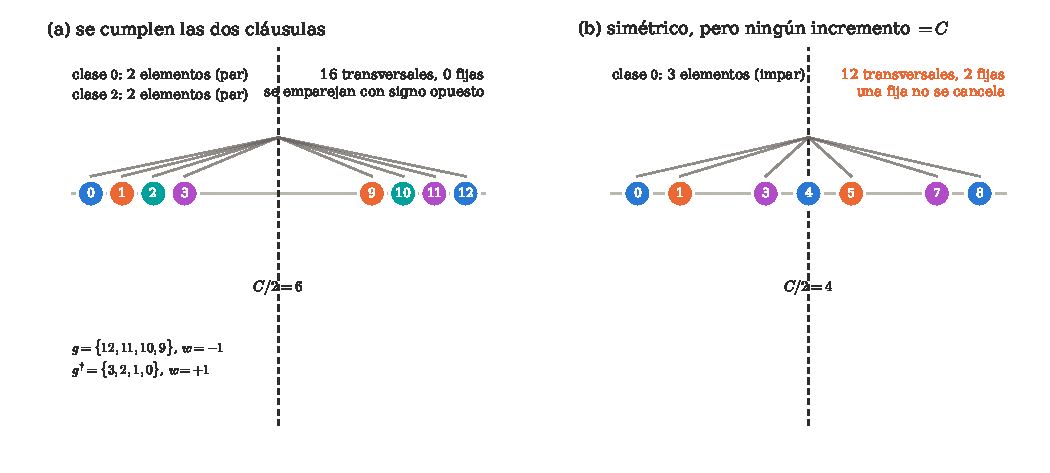
\includegraphics[width=\textwidth]{fig_pairing_es.pdf}
\caption{Por qué se cancela la suma, y para qué está la segunda cláusula. Cada panel dibuja
$\mathcal{S}$ sobre una recta, coloreado por clase de residuo, con un arco que une $v$ con $C-v$ y el
eje de puntos en $C/2$. \emph{(a)} $\beta=(12,11,10,9,3,2,1,0)$ con $t=4$, $r=2$: las dos clases que
la reflexión fija tienen tamaño \emph{par}, así que ninguna contiene a $C/2$; las $16$ transversales
se emparejan sin ningún punto fijo, y cada pareja lleva signos opuestos, de modo que cada término de
\eqref{eq:laplacegen} lo cancela otro. Una de esas parejas está impresa con sus dos signos,
calculados y no afirmados. \emph{(b)} una forma con $C-\mathcal{S}=\mathcal{S}$ pero sin ningún
incremento igual a $C$, encontrada buscándola y no elegida: allí la clase fija tiene tamaño
\emph{impar}, luego contiene a $C/2$, y dos transversales son su propio reflejo. Un término
emparejado consigo mismo no puede cancelarse, y la suma sobrevive. Eso es todo lo que compra la
segunda cláusula. Calculada por \texttt{anc/fig\_involution2.py}.}
\label{fig:pairing}
\end{figure}

\begin{lemma}[la transversal reflejada]\label{lem:reflact}
Supongamos $C-\mathcal{S}=\mathcal{S}$. Entonces $x\mapsto C-x$ lleva la clase $i$ sobre la clase
$i^{*}:=C-i \bmod t$, y o las dos están en $\mathcal{E}$ o ninguna; de modo que
\[
g^{\dagger}:=\bigl(C-(g\cap\mathcal{S})\bigr)\cup\bigl(g\setminus\mathcal{S}\bigr)
\]
es de nuevo una transversal, $g\mapsto g^{\dagger}$ es una involución sobre ellas, y
$T_{g^{\dagger}}=C-T_g$.
\end{lemma}

\begin{proof}
Todo elemento de la clase $i$ es $\equiv i$, así que $x\mapsto C-x$ lo manda dentro de la clase
$i^{*}$; como $C-\mathcal{S}=\mathcal{S}$ y la aplicación es inyectiva, lleva la clase $i$
\emph{sobre} la clase $i^{*}$ siempre que $i\in\mathcal{E}$, lo que obliga a $i^{*}\in\mathcal{E}$ y a
$n_i=n_{i^{*}}$. Las clases unitarias no se tocan: su único elemento está congelado en toda
transversal. Por último $T_{g^{\dagger}}=\mathcal{S}\setminus g^{\dagger}=C-(\mathcal{S}\setminus
g)=C-T_g$.
\end{proof}

\begin{lemma}[el menor reflejado]\label{lem:Arefl}
$A(C-T)=A(T)$ para todo $2r$-conjunto $T$ y todo $C$.
\end{lemma}

\begin{proof}
% Sin "=" en esta frase: TeX parte la formula en linea despues de la relacion y deja el signo
% colgando fuera del margen, y forzarla con \mbox la echa entera fuera.  Se dice con palabras.
Sacar $x_i^{C}$ de cada una de las $2r$ filas multiplica el determinante por el factor
$\prod_j z_j^{C}z_j^{-C}$, que vale $1$, y deja la matriz de $T$ con $x_i$ sustituido por
$x_i^{-1}$, que es la
matriz de $T$ con las dos filas de cada par recíproco intercambiadas: un signo $(-1)^{r}$.
Y listar $C-T$ en orden decreciente invierte el orden de las columnas, lo que aporta
$(-1)^{\binom{2r}{2}}$, es decir $(-1)^{r}$, porque $2r-1$ es impar. Los dos se cancelan.
\end{proof}

\noindent Los dos movimientos de esa prueba no son nuestros, y merece la pena decir de quién son,
porque son el instrumento adecuado y los elegimos por eso. Escalar cada fila por una potencia para
sustituir $x_i$ por $\bar x_i$, y luego invertir un bloque de columnas para recoger
$(-1)^{n(n-1)/2}$, es la maniobra que Ayyer y Behrend emplean sobre el bialternante de una forma
autocomplementaria \cite[\S3]{AB19}; ellos mismos describen sus pruebas como apoyadas sólo en las
expresiones determinantales ``y la aplicación de operaciones estándar con determinantes'', y ésta es
una de esas operaciones. Albion hace la misma inversión del lado de las raíces de la unidad
\cite{Alb23,Alb25}, y a nivel de caracteres el mismo hecho es la invariancia de $sp_\lambda$ bajo
$x_i\mapsto\bar x_i$, recogida en \cite{AB19} y puesta a trabajar en \cite{AF20}.

Conviene explicar por qué es útil aquí, porque es lo que hace corta toda la sección. A un menor
reflejado se le puede atacar desarrollándolo, y entonces habría que seguir término a término las
clases unitarias y las reflejadas --- que es como lo intentamos primero, y no se acaba nunca. La
maniobra de Ayyer y Behrend, en cambio, liquida la reflexión en \emph{dos} cálculos de signo que no
miran las entradas en ningún momento, y es robusta justo en el sentido que necesitamos: no usa en
ningún paso que se esté reflejando el alfabeto entero, así que sobrevive al aplicarse a una
\emph{parte} del conjunto beta, con el resto quieto. Esa robustez es la razón de que el Lema
\ref{lem:Arefl} ocupe cuatro líneas y no una sección, y pertenece a la herramienta y no a nosotros.
Es además un indicio menor a favor de la tesis de la \S\ref{sec:background}: las dos líneas entre las
que se sitúa este artículo comparten más maquinaria de lo que sus enunciados dejan ver.

El enunciado que sigue es el corazón combinatorio del argumento, y sólo necesita la primera cláusula
de \eqref{eq:suffcond}. Reflejar un conjunto beta \emph{entero} es clásico --- es la identidad de
complementación \eqref{eq:compl}, y los pasos determinantales que hay detrás son los estándar que
acabamos de citar. Lo que aquí se pide es la reflexión de la parte de exceso \emph{sola}, con las
clases unitarias quietas e intercaladas entre los valores reflejados; las dos involuciones que eso
produce, una de $\beta$ y otra de $\ZZ/t$, son de las que acaba dependiendo el signo.

\begin{lemma}[la fórmula del signo de la reflexión parcial]\label{lem:signformula}
Supongamos $C-\mathcal{S}=\mathcal{S}$, y pongamos
\[
\nu=\#\{x\in\mathcal{S}:2x=C\},\qquad \eta=\#\{i\in\mathcal{E}:2i\equiv C \bmod t\}.
\]
Entonces, para toda transversal $g$,
\begin{equation}\label{eq:wrefl}
\frac{w(g^{\dagger})}{w(g)}\;=\;(-1)^{\,e-\frac{\nu+\eta}{2}} .
\end{equation}
En particular el cociente no depende de $g$, ni de $r$, ni de $N$.
\end{lemma}

\begin{corollary}\label{cor:whenminus}
Bajo $C-\mathcal{S}=\mathcal{S}$, el cociente \eqref{eq:wrefl} vale $-1$ si y sólo si $\eta=2$.
\end{corollary}

\begin{proof}
Una involución tiene tantos puntos fijos como elementos su conjunto, módulo dos, así que
$\nu\equiv|\mathcal{S}|$ y $\eta\equiv e$; y $|\mathcal{S}|=2r+e$ por \eqref{eq:excessgen}, luego
también $\nu\equiv e$. Si $e$ es impar, entonces $\nu=\eta=1$ y el exponente es $e-1$, par. Si $e$ es
par, entonces $\nu=0$ y $\eta$ vale $0$ ó $2$, lo que da el exponente $e$ ó $e-1$; el primero es par y
el segundo impar.
\end{proof}

\noindent Esa independencia es la parte que parece improbable y es justo la que importa: las clases
unitarias están colocadas en posiciones arbitrarias entre los valores reflejados, y mover una
transversal las hace cruzarse unas con otras --- pero cada cruce que aportan a la suma de columnas lo
deshace el cruce que aportan a la palabra de residuos, así que no dejan rastro en el cociente.

\begin{lemma}[el signo reflejado]\label{lem:signrefl}
Supongamos \eqref{eq:suffcond}. Entonces $\eta=2$, el número $e$ es par, $\nu=0$, y
$w(g^{\dagger})=-w(g)$ para toda transversal $g$.
\end{lemma}

\begin{proof}[Prueba del Lema \ref{lem:signformula}]
Sea $\mathcal{R}$ la aplicación $x\mapsto C-x$ sobre $\mathcal{S}$ y la identidad sobre
$\beta\setminus\mathcal{S}$, y sea $\mathcal{R}_t$ la aplicación $i\mapsto i^{*}$ sobre $\mathcal{E}$
y la identidad fuera; ambas son involuciones, de $\beta$ y de $\ZZ/t$ respectivamente, con $\nu$ y
$\eta$ puntos fijos, así que $\sgn(\mathcal{R})=(-1)^{(|\mathcal{S}|-\nu)/2}$ y
$\sgn(\mathcal{R}_t)=(-1)^{(e-\eta)/2}$. Ordenemos las columnas de una transversal $g$ por residuo y
las restantes por $\beta$ decreciente; el signo de la permutación de $\{1,\dots,N\}$ que resulta es
$w(g)$ salvo un factor que depende sólo de $t$. Aplicar $\mathcal{R}$ a esa notación de una línea
aporta $\sgn(\mathcal{R})$; restablecer el orden por residuo del primer bloque aporta
$\sgn(\mathcal{R}_t)$; y $\mathcal{R}$ invierte $T_g$ por completo, de modo que restablecer su orden
decreciente aporta $(-1)^{\binom{2r}{2}}$. Multiplicando los tres sale \eqref{eq:wrefl}, donde ningún
término se refiere a $g$.
\end{proof}

\begin{proof}[Prueba del Lema \ref{lem:signrefl}]
Contar puntos fijos de una involución da $|\mathcal{S}|\equiv\nu$ y $e\equiv\eta \pmod 2$, y
$|\mathcal{S}|=2r+e$ por \eqref{eq:excessgen}, luego $e\equiv\nu$. Ahora bien, la segunda cláusula de
\eqref{eq:suffcond} dice que dos elementos \emph{adyacentes} de alguna clase $i_0$ suman $C$; la
reflexión los intercambia, así que $i_0=i_0^{*}$, y escribiendo la clase en orden decreciente el
intercambio manda su $k$-ésima entrada a la $(n_{i_0}+1-k)$-ésima, de donde $n_{i_0}=2k$ es par. La
reflexión $x\mapsto C-x$ tiene a lo sumo un punto fijo, que es $C/2$; como esta clase es estable bajo
ella y tiene cardinal par, sus elementos se emparejan y no contiene ninguno, luego $C/2\notin$ clase
$i_0$.

Antes de hablar de una segunda solución hay que saber que la hay, y ahí es donde la paridad de $t$ se
decide en vez de suponerse. Supongamos $t$ impar. Entonces $2$ es invertible módulo $t$, así que
$i\mapsto i^{*}$ tiene a $i_0$ como su \emph{único} residuo fijo; las demás clases de $\mathcal{E}$ se
emparejan, luego $e$ es impar, y $|\mathcal{S}|=2r+e$ también. Una involución sobre un conjunto de
tamaño impar tiene un punto fijo, así que $\nu=1$ y $C/2\in\mathcal{S}$; su residuo $\kappa$ cumple
$2\kappa\equiv C$, luego $\kappa=i_0$, lo que sitúa a $C/2$ en la clase $i_0$ --- que acabamos de ver
que no lo contiene. Así que $t$ es par, y $2i\equiv C$ tiene exactamente las dos soluciones $i_0$ e
$i_1=i_0+t/2$.

Si $\nu=1$, entonces $C/2\in\mathcal{S}$ y su residuo es $i_0$ o $i_1$; no es $i_0$, luego
$i_1\in\mathcal{E}$. Si $\nu=0$, entonces $e$ es par, y $\mathcal{E}=\{i_0\}\sqcup\{\text{pares}\}$
haría $e$ impar salvo que $i_1\in\mathcal{E}$. En cualquiera de los dos casos $\eta=2$, luego $e$ es
par y $\nu=0$, y el Corolario \ref{cor:whenminus} da el signo de inmediato. Leyendo \eqref{eq:wrefl}
directamente, el exponente es $e-\tfrac{0+2}2=e-1\equiv1 \pmod 2$.
\end{proof}

\begin{corollary}[la hipótesis, leída sobre los residuos]\label{cor:suffgeom}
Supongamos $C-\mathcal{S}=\mathcal{S}$. Entonces algún $\Delta_i(k)=C$ si y sólo si $t$ es par y
\emph{las dos} soluciones de $2i\equiv C \pmod t$ son clases de exceso. Dicho de otro modo,
\eqref{eq:suffcond} afirma: la parte de exceso del conjunto beta es simétrica respecto de $C/2$, y las
dos clases de residuos que la reflexión fija son ambas de exceso.
\end{corollary}

\begin{proof}
Una dirección es el primer párrafo de la prueba del Lema \ref{lem:signrefl}. Para la otra, si las dos
clases fijas están en $\mathcal{E}$ entonces $\eta=2$, luego $e$ es par por $e\equiv\eta$, luego
$|\mathcal{S}|=2r+e$ es par y $\nu=0$: ningún elemento de $\mathcal{S}$ queda fijo. Una clase fija es
entonces estable por la reflexión y sin puntos fijos, luego de tamaño par $2k$, y sus entradas
$k$-ésima y $(k+1)$-ésima se intercambian, así que $\Delta_i(k)=C$.
\end{proof}

\noindent Leída así, la hipótesis tiene la misma forma que la conclusión del Corolario
\ref{cor:Ctaugen}, y eso es lo que hace que las dos mitades de la sección se miren la una a la otra:
allí las dos clases empatadas \emph{resultan} ser las dos soluciones de $2\kappa\equiv C$; aquí
\emph{pedimos} que sean de exceso.

\begin{proof}[Prueba del Teorema \ref{thm:suff}]
Por el Lema \ref{lem:reflact}, $g\mapsto g^{\dagger}$ es una involución sobre las transversales con
$T_{g^{\dagger}}=C-T_g$. No tiene puntos fijos: una transversal fija necesitaría $C-g_i=g_i$, es
decir $g_i=C/2$, en toda clase con $i=i^{*}$, y la clase $i_0$ de la prueba anterior es una de ésas y
no contiene a $C/2$. Por los Lemas \ref{lem:Arefl} y \ref{lem:signrefl},
\[
w(g)A(T_g)+w(g^{\dagger})A(T_{g^{\dagger}})=w(g)A(T_g)-w(g)A(C-T_g)=0 ,
\]
así que la suma de \eqref{eq:laplacegen} se cancela por parejas y el numerador se anula
idénticamente.
\end{proof}

\begin{remark}[qué es esto, y qué no es]\label{rem:suffscope}
Conviene separar tres cosas. Primera: en $t=2$ la hipótesis \eqref{eq:suffcond} \emph{es} la rama
{\rm(b)}; allí $e=2$ obliga a $\mathcal{S}=\beta$, con lo que $C-\mathcal{S}=\mathcal{S}$ es la
autocomplementariedad, y la cláusula del incremento es la paridad de la anchura --- los dos enunciados
coinciden en todas las formas de los rangos de la \S\ref{sec:verif}. Así que el Teorema
\ref{thm:suff} contiene esa mitad del Teorema \ref{conj:crit}, y la prueba otra vez por un mecanismo
distinto. Segunda: para $t\ge4$ \emph{no} es complementación; allí $\mathcal{S}\subsetneq\beta$,
$\lambda$ no es autocomplementaria, y \eqref{eq:compl} no dice nada. Tercera: la involución es global
--- empareja \emph{todos} los términos de \eqref{eq:laplacegen} y no sólo los dos maximizadores ---, y
por eso sobrevive donde el argumento extremal sólo produce una condición necesaria.
\end{remark}

\begin{conjecture}[el criterio, en general]\label{conj:general}
Recíprocamente, si $\Phi_{t,r}(\lambda;z)\equiv0$ y toda clase de residuos está ocupada, entonces vale
\eqref{eq:suffcond}. Equivalentemente, para todo $t$ y todo $r$,
\[
\Phi_{t,r}(\lambda;z)\equiv0
\iff
\text{alguna clase es vacía, o } C-\mathcal{S}=\mathcal{S}\text{ y algún }\Delta_i(k)=C .
\]
\end{conjecture}

\noindent Bajo la hipótesis de anulación, casi todo lo que pide \eqref{eq:suffcond} ya se sabe, y
decir qué parte convierte la conjetura en una sola frase sobre un solo conjunto. El Corolario
\ref{cor:Ctaugen} da $C=\tau$, luego los incrementos empatados valen $C$ y la segunda cláusula se
cumple; y \eqref{eq:Ssymgen} da $C-(\mathcal{S}\setminus g_{\mathrm{com}})=\mathcal{S}\setminus
g_{\mathrm{com}}$. Como $\mathcal{S}=(\mathcal{S}\setminus g_{\mathrm{com}})\sqcup g_{\mathrm{com}}$,
lo único que queda es esto:

\begin{conjecture}[la parte común es simétrica]\label{conj:gcom}
Bajo ocupación, si $\Phi_{t,r}(\lambda;z)\equiv0$ entonces $C-g_{\mathrm{com}}=g_{\mathrm{com}}$.
\end{conjecture}

\noindent Las Conjeturas \ref{conj:general} y \ref{conj:gcom} son el mismo enunciado, y la segunda es
la forma útil: nombra los $e-2$ elementos a los que el argumento tiene que llegar, y ningunos más.
Dice también, de una vez, por qué $t=2$ cierra y $t\ge4$ no. En $t=2$ un empate es entre las clases
$i$ e $i+1$, de modo que las dos son de exceso y $e=2$ ---no porque allí $e=2$ valga siempre, pues
\eqref{eq:excessgen} permite $e=1$ y es frecuente, sino porque $|G|=2$ lo obliga, y
$g_{\mathrm{com}}$ sólo está definido cuando $|G|=2$---. Por tanto $g_{\mathrm{com}}=\varnothing$ y
no queda nada que pueda ser simétrico. El teorema no es allí más
fácil; sencillamente no hay parte común.

Los enunciamos como conjeturas y no como teoremas porque sólo está probada la dirección de arriba. La
evidencia está en la \S\ref{sec:verif}: sobre $190\,443$ formas en veinticuatro configuraciones, con
$t\le12$ y $r\le4$, el criterio no tiene ningún falso positivo ni ningún falso negativo; $43\,010$
de ellas se rehacen con una evaluación que no comparte código con esta sección, y un barrido más de
$12\,937$ formas, con $131$ ceros, se rehace en Sage, que no comparte con ninguna de las dos ni
código ni biblioteca; en los rangos donde ya
decide un teorema, coincide con el Teorema \ref{thm:main} en $r=1$ y con el Teorema \ref{conj:crit} en
$t=2$ sin una sola discrepancia, sobre $9913$ y $29\,508$ formas; y un señuelo que lee la condición
sobre $\beta$ en vez de sobre $\mathcal{S}$ --- esto es, la autocomplementariedad de la forma en lugar
de la de su parte de exceso --- falla en todas las configuraciones de ambos barridos. Lo que falta es
una implicación: el Corolario \ref{cor:necgen} da la reflexión sobre $\mathcal{S}\setminus
g_{\mathrm{com}}$, y el estrato superior no puede dar más --- hay formas que comparten $\tau$,
$\mathcal{S}\setminus g_{\mathrm{com}}$ y las clases empatadas, y de las cuales unas se anulan y otras
no, así que la ecuación que falta no es un refinamiento de la \S\ref{sec:rigidity} sino un enunciado
sobre un estrato inferior.

\begin{remark}[por qué no el argumento obvio]
Lo primero que se intenta es un intercambio dentro de un \emph{solo} maximizador: si
$\max\mathcal{S}$ está omitido, re-elegir su clase y esperar que suba el grado. No puede funcionar.
Un maximizador puede omitir $\max\mathcal{S}$ --- justo cuando $\max\mathcal{S}$ es uno de los valores
empatados $p_1,p_2$, de modo que un maximizador lo omite y el otro lo conserva ---, así que ningún
argumento que lea una transversal cada vez concluye. La Proposición \ref{prop:A1gen} es un enunciado
sobre el \emph{par}, y por eso la prueba corre sobre \eqref{eq:halvesgen} y sobre nada más. El Cuadro
\ref{tab:extremal} recoge tanto los pasos de esa prueba como lo que le pasa a su conclusión cuando se
quita la hipótesis.
\end{remark}

\begin{table}[!ht]
\centering\small
\caption{La maquinaria de las \S\S\ref{sec:extremal}--\ref{sec:rigidity}, medida. La población es
toda forma con $|G|=2$ sobre $(t,r)\in\{4,6,8,10\}\times\{2,3\}$ dentro de las anchuras barridas. La
última fila es la que importa para la Proposición \ref{prop:A1gen}: al quitar la hipótesis
$[\det]_{D_1}=0$ la conclusión falla, así que no viene de balde.}
\label{tab:extremal}
\begin{tabular}{@{}llrl@{}}
\toprule
enunciado & población & resultado & guion \\
\midrule
\rowcolor{hband} parametrización voraz $=$ fuerza bruta & $4049$ formas & \textcolor{hproved}{$0$ fallos} & \texttt{a1\_proof} \\
$A$ es la mitad de arriba de $T_g$ (Paso 2) & la misma & \textcolor{hproved}{$0$ fallos} & \texttt{a1\_proof} \\
\rowcolor{hband} $T_{\mathrm b}=\tau-T_{\mathrm a}$ & $2522$ formas & \textcolor{hproved}{$0$ fallos} & \texttt{a1\_proof} \\
$v\in L_{\mathrm b}\Rightarrow\tau-v\in H_{\mathrm a}$ & $3034$ valores & \textcolor{hproved}{$0$ fallos} & \texttt{a1\_proof} \\
\rowcolor{hband} los extremos evitan $g_{\mathrm{com}}$ & $2522$ formas & \textcolor{hproved}{$0$ fallos} & \texttt{a1\_proof} \\
las identidades mostradas de estas subsecciones & $11$ identidades & \textcolor{hproved}{$0$ fallos} & \texttt{v2\_formulas} \\
\midrule
\rowcolor{hband} lo mismo, quitando $[\det]_{D_1}=0$ & $24718$ formas & \textcolor{hverif}{$414$ fallos} & \texttt{a1\_proof} \\
\bottomrule
\end{tabular}
\end{table}

\begin{remark}
El Corolario \ref{cor:reflectgen} hace trabajo de verdad en la Proposición \ref{prop:A1gen}, y
$|G|=2$ por sí solo no basta. Para $t=4$, $r=2$ y $\beta=(200,199,198,197,194,193,191,4)$ las clases
de exceso son $\{200,4\}$, $\{197,193\}$, $\{198,194\}$, $\{199,191\}$ y los incrementos son
$392,390,390,204$, así que $\tau=390$, el empate es entre las clases $1$ y $3$, y $|G|=2$. Pero
$\Delta_0(1)=204<\tau$, así que $k_0=0$ en los dos maximizadores y $\max\mathcal{S}=200$ lo omiten los
dos: la conclusión de la Proposición \ref{prop:A1gen} falla. Aquí $T_{\mathrm a}=(198,197,191,4)$ y
$T_{\mathrm b}=(199,198,193,4)$ no son reflexión una de otra --- $h_r-l_1$ vale $6$ para la primera y
$5$ para la segunda --- y en consecuencia la componente de grado $D_1$ no se anula.
\end{remark}

\begin{figure}[!ht]
\centering
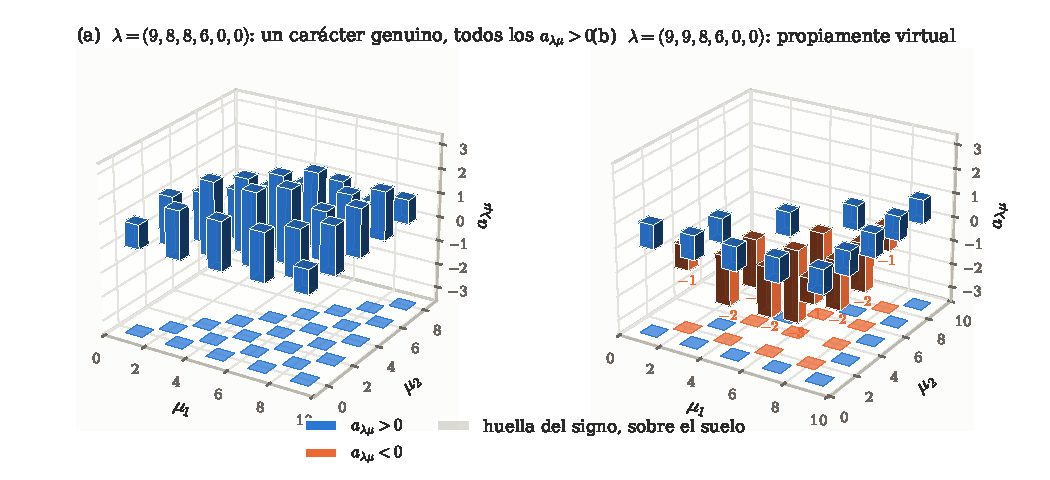
\includegraphics[width=\textwidth]{fig_virtual_es.pdf}
\caption{Por qué un solo par recíproco no es lo típico, en $r=2$: la expansión
$\Psi_r(\lambda)=\sum_\mu a_{\lambda\mu}\,sp_\mu(z)$ sobre los pesos dominantes de $Sp(4)$. Las dos
formas difieren en una sola casilla. Para $\lambda=(9,8,8,6,0,0)$ todo $a_{\lambda\mu}$ es positivo:
el objeto es un carácter genuino, como lo es para \emph{toda} $\lambda$ cuando $r=1$, donde el
Teorema \ref{thm:main} lo escribe como producto de tres caracteres de $\mathfrak{sl}_2$. Para
$\lambda=(9,9,8,6,0,0)$ la expansión tiene $12$ coeficientes positivos y $10$ negativos, siendo el más
negativo $-3$: es genuinamente virtual, que es el fenómeno que recoge la Observación
\ref{rem:rankone} y la razón de que un cálculo en el extremo deje de ser un test exacto pasado un
par. Los dos paneles comparten la escala vertical, y los cuadrados planos del suelo repiten el signo
de cada coeficiente, porque un coeficiente $-1$ es invisible al lado de uno $+3$. Calculada por
\texttt{anc/fig\_v2.py}.}
\label{fig:virtual}
\end{figure}

\subsubsection*{El criterio en \texorpdfstring{$t=2$}{t=2}}

\begin{proof}[Demostración del Teorema \ref{conj:crit}]
La implicación de (a) o (b) a $\Psi_r(\lambda)=0$ es el Teorema \ref{thm:zeros}. Para el recíproco,
supóngase $\Psi_r(\lambda)=\Phi_{2,r}(\lambda;z)\equiv0$ y que ninguna clase de residuos módulo $2$
falta en $\beta(\lambda)$, ya que en otro caso se cumple la rama (a) y no hay nada que probar.
Entonces el numerador se anula idénticamente, así que en particular su componente de grado $D_1$ se
anula y $|G|=2$ por el Corolario \ref{cor:uniquegen}.

Por el Teorema \ref{thm:Ggen}(b) hay un empate en el rango $r$ entre las clases $i$ e $i+t/2=i+1$; en
$t=2$ ésas son las dos clases, y ambas están en $\mathcal{E}$, luego $e=2$. (Con $e=1$ todos los
incrementos viven en una sola clase y son distintos dos a dos por el Paso 4, así que no hay empate
posible.) Como $e=2$, ninguna clase es unitaria y $\mathcal{S}=\{\beta_1,\dots,\beta_N\}$ es el
beta-conjunto entero.

Por el Corolario \ref{cor:Ctaugen}, $C=\min\mathcal{S}+\max\mathcal{S}=\beta_N+\beta_1=\tau$ y, como
cambian las dos clases, $g_{\mathrm{com}}=\varnothing$ en \eqref{eq:gcomgen}, de modo que
\eqref{eq:Ssymgen} se lee $\tau-\mathcal{S}=\mathcal{S}$: el beta-conjunto es simétrico respecto de
$C$, es decir
\[
  \beta_j+\beta_{N+1-j}=C\qquad\text{para todo }j .
\]
Sustituyendo $\beta_j=\lambda_j+N-j$ esto se convierte en $\lambda_j+\lambda_{N+1-j}=C-N+1=:w$ para
todo $j$, que es la auto-complementariedad de anchura $w=\lambda_1+\lambda_N$. Finalmente, el
Corolario \ref{cor:Ctaugen} dice que las dos soluciones de $2\kappa\equiv C\pmod2$ son las dos
clases, lo que ocurre exactamente cuando $C$ es par; y $C=w+N-1$ con $N=2r+2$ par, así que $C$ par es
exactamente $w$ impar. Luego $\lambda$ es auto-complementaria de anchura impar: la rama (b).
\end{proof}

\begin{remark}
En $t=2$ la congruencia \eqref{eq:congrgen} es vacua --- todo incremento es par --- y $|G|\le2$ vale
por la razón más débil de que sólo existen dos clases. Lo que \emph{no} es vacuo en $t=2$ es que
$\tau$ sea par, y se usa dos veces: prohíbe el emparejamiento cruzado en la Proposición
\ref{prop:centregen}, y \emph{es} la paridad que se convierte en la rama (b).
\end{remark}

\begin{remark}[\emph{genuino} no quiere decir \emph{irreducible}]
En la Observación \ref{rem:rankone}, \emph{$\pm$ un carácter genuino} significa una combinación
\emph{no negativa} de irreducibles, no uno solo. No es uno solo: ya
$s_{(2)}(1,-1,z,z^{-1})=z^{2}+2+z^{-2}=sp_{(2)}+sp_{(0)}$. En $t=2$, $r=1$ el Teorema
\ref{thm:main} da un producto de tres caracteres de $\mathfrak{sl}_2$, y un producto de caracteres es
un carácter --- ésa es toda la afirmación. A partir de $r=2$ aparecen coeficientes negativos y no
existe ninguna representación, que es lo que quiere decir \emph{genuinamente virtual}; el Cuadro
\ref{tab:virtual} cuenta las dos cosas y la Figura \ref{fig:virtual} dibuja una de cada.
\end{remark}

\begin{table}[!ht]
\centering\small
\caption{Genuino frente a genuinamente virtual, sobre todas las $\lambda$ con $\lambda_1$ hasta la
cota indicada. La expansión es $\Psi_r(\lambda)=\sum_\mu a_{\lambda\mu}\,sp_\mu(z)$; \emph{un signo}
quiere decir que todos los $a_{\lambda\mu}$ tienen el mismo signo, de modo que $\pm\Psi_r$ es un
carácter, y \emph{mezclado} quiere decir que es genuinamente virtual. En $r=1$ la columna de mezclados
está vacía, como fuerza el Teorema \ref{thm:main}; no lo está para ningún $r\ge2$ al que lleguemos.
Calculada por \texttt{anc/fig\_v2.py}.}
\label{tab:virtual}
\begin{tabular}{@{}lrrrr@{}}
\toprule
 & \multicolumn{1}{c}{formas} & \multicolumn{1}{c}{$\Psi_r=0$} & \multicolumn{1}{c}{un signo}
 & \multicolumn{1}{c}{mezclado} \\
\midrule
\rowcolor{hband} $r=1$, $\lambda_1\le14$ & $3060$ & $352$ & $2708$ & \textcolor{hproved}{$\mathbf{0}$} \\
$r=2$, $\lambda_1\le8$  & $3003$ & $78$ & $2531$ & \textcolor{hverif}{$\mathbf{394}$} \\
$r=3$, $\lambda_1\le5$  & $1287$ & $27$ & $1008$ & \textcolor{hverif}{$\mathbf{252}$} \\
$r=4$, $\lambda_1\le2$  & $66$   & $2$  & $58$   & \textcolor{hverif}{$\mathbf{6}$} \\
\bottomrule
\end{tabular}
\end{table}

\begin{remark}[dónde vive el alfabeto]
Para $r=1$ el alfabeto $(1,-1,z,\bar z)$ de \eqref{eq:psir} es literalmente la lista de valores
propios de una matriz de la componente no identidad $O(4)^{-}$, tabulada como tal por Hanany y
Kalveks \cite[Tabla 7]{HK16}, que además registran la caída de rango
$[\mathrm{vec}]_{O(2n)^{-}}\cong[\mathrm{vec}]_{O(2)^{-}}\oplus[\mathrm{fund}]_{C_{n-1}}$ para la
representación \emph{vectorial}. Así que $\Psi_r$ es un carácter de $GL(2r+2)$ evaluado en esa
componente, y el plegado $D_{r+1}\to C_r$ es la razón de que aparezca un grupo simpléctico; no lo
usamos más que para situar el objeto, ya que para una $\lambda$ cualquiera la restricción es una
combinación con coeficientes enteros de caracteres simplécticos, y no uno solo.
\end{remark}

\section{Verificación}\label{sec:verif}

Todos los enunciados anteriores se comprobaron numéricamente, con tres implementaciones por rutas de
código distintas: una en aritmética de Laurent exacta, otra una evaluación del bialternante escrita
desde cero a partir de los enunciados, y una tercera en Sage, que no comparte con las otras dos ni
una línea de código ni una biblioteca. Los rangos y recuentos se recogen aquí una sola vez.

% longtable y no tabular: con un tabular esta tabla es una caja indivisible, y LaTeX la empuja
% entera a la pagina siguiente dejando la de la cabecera de seccion casi vacia.  longtable parte por
% paginas y repite la cabecera, que es lo que una tabla de cuarenta filas necesita.
% \raggedright en las dos primeras: justificadas, una columna estrecha estira los espacios y deja
% "t <= 7, |lambda| <=" con huecos enormes.  La tercera va \raggedleft porque son cifras.
\begingroup\footnotesize\setlength{\tabcolsep}{4.0pt}
% Anchuras algo menores que en la edicion inglesa: el castellano es mas largo por palabra y con las
% de alla la tabla se salia 4 pt.  Se miden en el PDF, no en el log.
\begin{longtable}{@{}>{\raggedright\arraybackslash}p{0.352\linewidth}%
                  >{\raggedright\arraybackslash}p{0.222\linewidth}%
                  >{\raggedleft\arraybackslash}p{0.272\linewidth}@{\hspace{4pt}}l@{}}
\toprule
enunciado & rango & resultado & estado\\
\midrule
\endfirsthead
\multicolumn{4}{@{}l}{\footnotesize\itshape Verificación, continuación}\\[1pt]
\toprule
enunciado & rango & resultado & estado\\
\midrule
\endhead
\midrule
\multicolumn{4}{r@{}}{\footnotesize\itshape sigue en la página siguiente}\\
\endfoot
\bottomrule
\endlastfoot
Teor. \ref{thm:main}, signo incluido & $t\le7$, $|\lambda|\le14,\dots,10$ &
$959$ exactos, $476$ ceros, $0$ fallos & \stproved\\
\quad lo mismo, una implementación escrita desde el enunciado & $t\le6$, $|\lambda|\le12,\dots,9$ &
$749$ formas, $0$ fallos; el señuelo del signo falla $35/133$ & \stproved\\
Lema \ref{lem:L1} & $t\le6$ & $454$ menores no nulos & \stproved\\
Lema \ref{lem:L4} & $t\le7$ & $724/724$ & \stproved\\
Proposición \ref{prop:quotient} & $t\le7$, $|\lambda|\le19$ & $2970/2970$ & \stproved\\
Prop. \ref{rem:lattice} (lugar concéntrico) & $t\le9$, $|\lambda|\le16$ & $1331/1331$;
$0$ con $t$ impar, $43$ con par & \stproved\\
Prop. \ref{rem:sign} (forma corta del signo) & $t\le8$, $|\lambda|\le14$ & $1496/1496$;
pasos de la prueba, $0$ fallos & \stproved\\
\quad la ley de desplazamiento \eqref{eq:shift} y su signo & $t\le7$, $|\lambda|\le12$ &
$826$ formas, $0$ fallos & \stproved\\
Prop. \ref{prop:minimal} (el multiconjunto separa) & $d_i\le60$; $t\le5$, $|\lambda|\le16$ &
$75640$ invariantes, $0$ colisiones & \stproved\\
\quad lo mismo, en los dos sentidos, desde el enunciado & $t\le5$, $|\lambda|\le14,\dots,11$ &
$676$ formas, $0$ colisiones; señuelo $104$ & \stproved\\
Prop. \ref{prop:fibrelattice} (el retículo) & $t\le5$, $|\lambda|\le14,12,10,10$ &
$84$, $35$, $20$, $14$ fibras, en ambos sentidos & \stproved\\
Cor. \ref{cor:fibregf} (función generatriz) & mismo rango &
$153/153$; denominador erróneo $101$ & \stproved\\
Observación \ref{rem:signsees} (el signo ve los $m_i$) & $t\le4$ &
$107/107$, $43/62$, $26/36$ & \stverif\\
Lema \ref{lem:single} & $t\le7$, $|\lambda|\le16$ & $2113/2113$ & \stproved\\
Teor. \ref{thm:extra} & $t\le12$, $\lambda_1\le33$ & $119+21$, ninguna más & \stproved\\
\quad el signo es $+1$, \eqref{eq:extrainv} & $t\le14$ par; núcleos $t\le10$ &
$28$ extra $+$ $219$ núcleos, todos $+1$ & \stproved\\
Proposición \ref{prop:rect} & $t=2$, $r\le4$, $c\le60$ & $240/240$ & \stproved\\
Cor. \ref{cor:enum} contra enumeración directa & $t\le5$ & $14/14$; cajas $16/16$ &
\stproved\\
Prop. \ref{rem:involution} (las rachas alternan) & $t=2$, $|\lambda|\le14$, $\le4$ filas &
$4823$ menores; $217$ pares, $0$ fallos & \stproved\\
(D3), (D4) de la \S\ref{sec:sharp} & $t\le6$, $|\lambda|\le10$ &
$600$ / $383$ / $200$ de $600$ & \stverif\\
\midrule
\rowcolor{hband} Teor. \ref{conj:crit}, el criterio, todo $r$ & --- & prueba, \S\ref{sec:rigidity} & \stproved\\
\rowcolor{hband} \quad lo mismo, leído sobre $O(N)$, Cor.~\ref{cor:dettwist} & --- &
reformulación, \S\ref{sec:conv} & \stproved\\
\rowcolor{hband} \quad Teor. \ref{thm:PvW}, el input externo & --- & \cite{PvW} & \stext\\
\rowcolor{hband} \quad Teorema \ref{thm:Ggen}, $|G|\le2$ & $t\le10$, $r\le3$ & voraz contra fuerza bruta, $0/4049$ & \stproved\\
\rowcolor{hband} \quad Prop.~\ref{prop:A1gen}, los extremos & $t\le10$, $r\le3$ & $2522$ formas, $0$ fallos & \stproved\\
\rowcolor{hband} \quad \quad la hipótesis hace falta & mismo & $414$ formas fallan sin ella & \stproved\\
\rowcolor{hband} \quad las identidades mostradas, \S\S\ref{sec:extremal}--\ref{sec:rigidity} & $t=2$, $r\le3$ & $11$ identidades, $0$ fallos & \stverif\\
\rowcolor{hband} Lema \ref{lem:step}, movimiento de columna, toda clase & $t\le6$, $r\le3$ &
$285\,600/285\,600$; señuelo de un término $149\,652$ & \stproved\\
\rowcolor{hband} Teor. \ref{thm:suff}, la dirección suficiente & $t\le8$, $r\le4$ &
$438$ formas, $0$ fallos; \eqref{eq:wrefl} $438/438$ & \stproved\\
\rowcolor{hband} Conj. \ref{conj:general}, ambas direcciones & $t\le12$, $r\le4$ &
$190\,443$ formas, $24$ configuraciones, $0$ fallos & \stverif\\
\rowcolor{hband} \quad lo mismo, evaluación independiente & $t\le8$, $r\le4$ &
$43\,010$ formas, $409$ ceros, $0$ fallos & \stverif\\
\rowcolor{hband} \quad lo mismo otra vez, en Sage & $t\le8$, $r\le3$ &
$12\,937$ formas, $131$ ceros, $0$ fallos & \stverif\\
\rowcolor{hband} \quad contra los Teoremas \ref{thm:main} y \ref{conj:crit} & $r=1$; $t=2$ &
$9913$ y $29\,508$ formas, $0$ discrepancias & \stproved\\
\rowcolor{hband} \quad el señuelo que lee $\beta$ en vez de $\mathcal{S}$ & mismo &
falla en $24$ de $24$ y en $14$ de $14$ & \stproved\\
\midrule
\rowcolor{hband} Teor. \ref{conj:crit}, ambas direcciones, comprobación directa & $r\le3$, $|\lambda|\le28,26,22$ &
$9961$ formas, $318$ ceros, $0$ fallos & \stproved\\
\rowcolor{hband} \quad rama (a), Teor.~\ref{thm:zeros} & $r\le3$, $|\lambda|\le15$ &
$16/16$ & \stproved\\
\rowcolor{hband} \quad rama (b), Teor.~\ref{thm:zeros} & $r\le3$ & $24/24$ & \stproved\\
\rowcolor{hband} \quad control de anchura par para (b) & $r\le3$ & $56/56$ no nulos & \stproved\\
\rowcolor{hband} \quad recíproco en $r=1$, Teor.~\ref{thm:r1} & $\beta_1\le25$ &
$14950$ conjuntos beta, $0$ fallos & \stproved\\
\rowcolor{hband} \quad recíproco, $\ell(\lambda)\le N/2$, Teor.~\ref{thm:stable} & $r\le3$ &
$372/372$ testigos & \stproved\\
\rowcolor{hband} \quad el testigo aislante, Prop.~\ref{conj:iso} & $r=2$, $|\lambda|\le14$ &
$227$ testigos, $11$ de residuo & \stproved\\
\rowcolor{hband} \quad lo mismo en $r=3$ & $r=3$, $|\lambda|\le13$ &
$149$ testigos, $0$ de residuo & \stproved\\
\midrule
Identidad \eqref{eq:compl} & $r\le2$ & $474/474$ & \stproved\\
Identidad \eqref{eq:docagne}, y $\deg_{c_\ast}S_n=n-1$ & $b\le31$ & $496/496$; $39/39$ &
\stproved\\
Lema \ref{lem:AtoSp}, la reducción de la \S\ref{sec:unstable} & $r\le3$, $|\nu|\le8$ &
identidad $0$ fallos; plegados $0$ fallos & \stproved\\
\quad la reducción, llevada a cabo & $r\le2$ & $236$ etiquetas, $0$ sin resolver & \stproved\\
\eqref{eq:Cmu} contra el objeto exacto & $r\le2$, ambos rangos & $184$ formas, $0$ fallos &
\stverif\\
\end{longtable}
\endgroup

\noindent El bloque sombreado es el Teorema \ref{thm:zeros} leído de arriba abajo: las dos ramas
suficientes están demostradas para todo $r$, el recíproco está demostrado para un par y, para todo
$r$, dentro del rango de Littlewood; y la línea que solía quedar ---el recíproco para $r\ge2$ fuera
de ese rango y más allá de la franja $|\lambda|\le2r+2$ que resuelve el Lema \ref{lem:nonstd}---
es el Teorema \ref{conj:crit}, demostrado en la \S\ref{sec:rigidity} por un argumento que no entra
en el rango de Littlewood. Por eso el bloque lleva ya \stproved\ en todas sus filas, con una en
\stext\ para el apoyo ajeno del que depende. La fila que registra lo que hace y lo que no hace el
certificado que propusimos se queda, y lleva \stproved\ porque la Proposición \ref{conj:iso} es un
contraejemplo y los contraejemplos son demostraciones; lo que acota ahora es una vía, no el
enunciado. Las filas por debajo del bloque son las identidades y la reducción sobre
las que se apoya la sección. En la columna, \stproved\ significa que aquí se da una demostración o se
cita, y \stverif\ que el enunciado se comprueba de forma exhaustiva sobre el rango indicado y no se
demuestra.

\noindent La fila de (D3), (D4) es la que más importa del primer grupo: la identidad se cumple en los
$600$ casos para \eqref{eq:object} y falla en $217$ y $400$ de ellos para los dos alfabetos
deformados, de modo que el contraste es capaz de fallar. En el segundo grupo, el control de anchura
par cumple el mismo papel para el Teorema \ref{thm:zeros}: $56$ formas autocomplementarias de anchura
par, ninguna de las cuales se anula, así que la hipótesis de paridad trabaja en lugar de decorar. Una
auditoría aparte reconstruye todo el segundo grupo desde las definiciones en una sola pasada, con
independencia de los guiones que los produjeron: $3414$ comprobaciones, $0$ fallos. Una segunda toma
las \emph{fórmulas mostradas} en vez de los recuentos ---el Teorema \ref{thm:LR}, la lectura por
intervalos \eqref{eq:intervals}, los Lemas \ref{lem:L2} y \ref{lem:L5}, la partición
\eqref{eq:threestep}, la complementación \eqref{eq:compl}, d'Ocagne \eqref{eq:docagne} y la
advertencia escalar \eqref{eq:scalar}--- y evalúa ambos miembros en puntos numéricos desde las
definiciones, sin usar ni las formas cerradas de este artículo ni los guiones que sostienen la
tabla: $3297$ evaluaciones sobre nueve fórmulas mostradas, $0$ fallos. Los guiones son
material auxiliar de este artículo, y también lo es la salida guardada de cada uno, de modo que todo
recuento de la tabla anterior puede localizarse en una ejecución archivada en lugar de aceptarse por
confianza.

%======================================================================
\section{Problemas abiertos}\label{sec:open}

La Figura \ref{fig:map} sitúa lo que sigue frente a lo que el artículo demuestra y lo que toma
prestado; los problemas de abajo son las cajas que deja abiertas.

\begin{figure}[!ht]
\centering
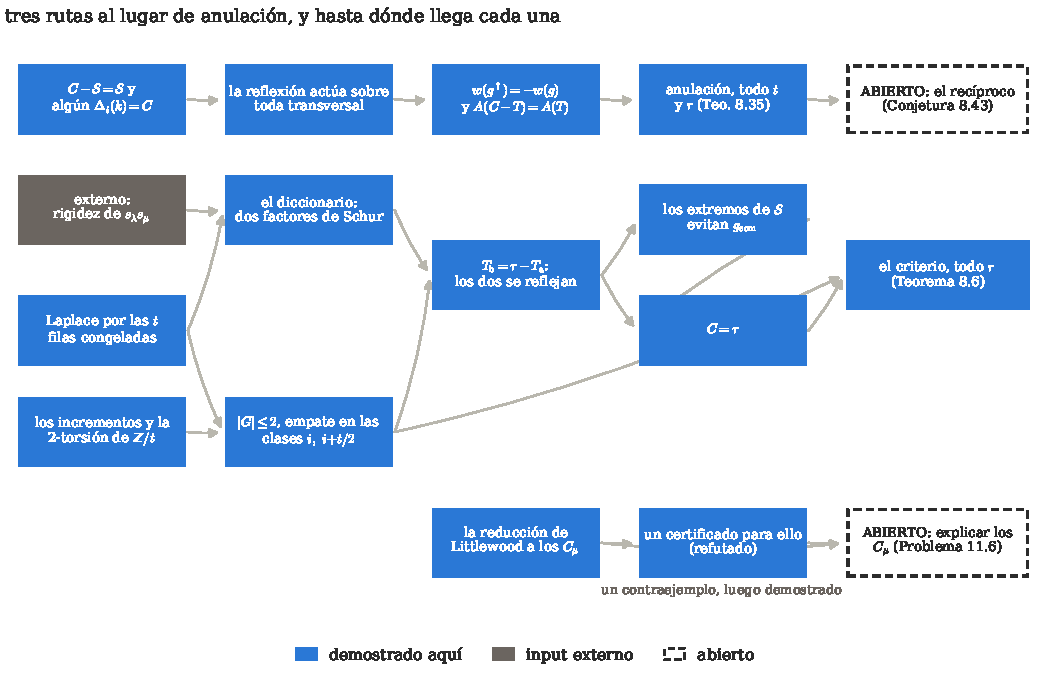
\includegraphics[width=\textwidth]{fig_map_es.pdf}
\caption{Sobre qué se apoya el criterio de la \S\ref{sec:zeros} y qué queda. Las cajas son
enunciados y las flechas dependencias; el color es la columna de estado de la \S\ref{sec:verif} ---
relleno lo demostrado aquí, gris el único apoyo ajeno, discontinuo lo abierto. La rama de arriba es
el argumento extremal de las \S\S\ref{sec:extremal} y \ref{sec:rigidity}; la de abajo es la
reducción de Littlewood, cuyo certificado refuta la Proposición \ref{conj:iso} ---un contraejemplo,
o sea una demostración---, de modo que la rama de abajo ya no toca el criterio sino la cuestión
aparte de explicar los $C_\mu$, que es el Problema \ref{prob:instrument}. Los enunciados van por
nombre y no por número, para que la figura no pueda desfasarse cuando la numeración lo haga.
Calculada por \texttt{anc/fig\_proof.py}.}
\label{fig:map}
\end{figure}

\begin{problem}[los otros tipos clásicos]\label{prob:types}
Todo lo anterior es de tipo $A$. ¿Qué hacen $sp_\lambda(\zt,z,\zb)$, $so_\lambda(\zt,z,\zb)$ y
$o_\lambda(\zt,z,\zb)$? Las factorizaciones de raíces de la unidad se llevaron del tipo $A$ a los
tipos $B$, $C$, $D$ con un argumento uniforme en \cite{AK22} y a los caracteres universales en
\cite{Alb23}; las filas congeladas del bialternante son las mismas en todos los tipos, de modo que el
Lema \ref{lem:L1} y el recuento de exceso dos deberían sobrevivir palabra por palabra, mientras que
el colapso, los Lemas \ref{lem:L4} y \ref{lem:L5}, habría que rehacerlo una vez por tipo. El alfabeto
\eqref{eq:object} es ya un elemento del toro de $O(t+2)$, de modo que los otros tipos no son la misma
función en un punto nuevo sino objetos nuevos, y elegir los correctos es cuestión de criterio dentro
de un programa que no hemos construido nosotros. Sí hemos medido, y lo damos como medición y nada
más. Desarrollando los caracteres universales de Koike--Terada en la base de Schur y evaluando
término a término con el Teorema \ref{thm:main}, sobre $|\lambda|\le12$ para $t\le3$ y
$|\lambda|\le10$ para $t=4,5$, la fracción de formas con $\ell(\lambda)\ge2$ en las que el valor se
anula es netamente mayor para $o_\lambda$ en la componente no identidad que en la identidad ---el
$83.8\%$ con $t=2$ frente al $41.8\%$ con $t=3$, y el $58.8\%$ con $t=4$ frente al $42.1\%$ con
$t=5$---, con $sp_\lambda$ en medio y el caso de Schur el más bajo. El efecto es real y sigue a la
componente, que es lo que cabría esperar de una cancelación entre asociados; pero es cuantitativo y
no le hemos encontrado ley que cubra la tabla entera. Un primer intento de ley, que $o_\lambda$ se
anule para todo
$\ell(\lambda)\ge2$ cuando $t$ es par, es falso: se leyó de una muestra y el barrido sistemático lo
refuta.

La columna $t=2$ de esa comparación es el único caso que sí tiene ley, y es el Lema
\ref{lem:AtoSp}: allí el alfabeto es \eqref{eq:psir} con $r=1$, de modo que $o_\nu$ es igual a
$sp_\nu(z)$, un carácter simpléctico de \emph{rango uno}. Ése se anula idénticamente para
$\ell(\nu)=2$ --- las $36$ formas del rango, sin excepción --- y se pliega para $\ell(\nu)>2$, que es
la razón de que la cifra de $t=2$ sea la que se sale. Lo que queda sin ley es $t$ impar, donde el
alfabeto no tiene la forma \eqref{eq:psir} y el lema no se aplica.

La columna de $sp_\lambda$ en $t=2$, en cambio, sí tiene respuesta, y explica la asimetría de la
tabla en lugar de añadirle una fila. Adjuntar esas mismas dos letras a un carácter universal
\emph{simpléctico} no lo colapsa. Sobre $|\nu|\le8$,
\begin{equation}\label{eq:spbranch}
sp_\nu(W,1,-1)\;=\;\sum_{\gamma\subseteq\nu}c_{\nu/\gamma}\;sp_\gamma(W),
\end{equation}
donde el coeficiente depende de $\nu$ y $\gamma$ solo a través de la forma sesgada $\nu/\gamma$
---$247$ coeficientes sobre $74$ formas sesgadas distintas, sin un solo choque--- y toma únicamente
los valores $0$ y $\pm1$, anulándose siempre que $|\nu/\gamma|$ es impar. Esa es la forma que produce
una regla de ramificación para funciones simplécticas universales, y tales reglas existen
\cite{JJLW24}. Leído contra ella, el Lema \ref{lem:AtoSp} dice que para $o_\nu$ los coeficientes
correspondientes se concentran en $\gamma=\nu$: las dos letras colapsan el carácter ortogonal a un
único carácter simpléctico, y dejan el simpléctico repartido por todo el intervalo bajo $\nu$. La
asimetría de la medición es eso, y no un artefacto de los rangos. Lo que no hemos hecho es
identificar $c_{\nu/\gamma}$, que \eqref{eq:spbranch} convierte en una pregunta sobre caracteres
simplécticos universales sesgados en $(1,-1)$ y en nada más.

La tercera columna se resiste a la misma vía, y por una razón estructural y no accidental. Lo que
resuelve las otras dos es que adjuntar una letra es el mapa de anillos $p_k\mapsto p_k+c^k$, de modo
que $\iota_{1}$ y $\iota_{-1}$ actúan sobre $\Lambda$ y componen. La identidad que traería $so$ al
cuadro, $so_\nu(X)=o_\nu(X,\bar X,1,0,\dots)$ de \cite[(2.13)]{AK25}, relaciona ambos sobre un
alfabeto \emph{duplicado}, y una duplicación no es una adjunción: los $\iota$ no llegan. Así que la
columna $so$ no es una laguna de esfuerzo sino de mecanismo, y la dejamos enunciada como tal.
\end{problem}

\begin{problem}[una Verschiebung que vea un par recíproco]\label{prob:versch}
El operador $\varphi_t$ no tiene nada que decir sobre una letra fuera de una $\zeta$-órbita, que es
la razón estructural de que el Teorema \ref{thm:main} no sea corolario de nada de esa línea, y la
razón de que nuestra demostración descienda al alternante. ¿Existe un operador sobre caracteres
universales, o una factorización de $\varphi_t$ a través de un álgebra mayor, que actúe sobre
alfabetos de la forma (unión de $\zeta$-órbitas) $\cup$ (pares recíprocos)? Por la \S\ref{sec:sharp},
un operador así decidiría (D1) y (D2) de una vez. La discusión de allí sugiere una forma
cuantitativa.

Lo que vuelve bien planteada la pregunta, y no vaga, es que cada mitad tiene ya un formalismo, y no
son el mismo. Las $\zeta$-órbitas son territorio de $\varphi_t$, en la formulación de Albion
\cite{Alb23}. Los alfabetos cerrados por inversión son territorio de las funciones simplécticas y
ortogonales universales, que admiten realizaciones por operadores de vértice de las que se siguen sus
reglas de ramificación \cite{JJLW24}. Nuestro alfabeto es uno de cada, y el Lema \ref{lem:AtoSp} es
el único sitio donde ambos se encuentran: allí la $\zeta$-órbita es $\{1,-1\}$, lo bastante pequeña
como para que adjuntarla sea un par de mapas de letra y no un operador. No conocemos nada que actúe
sobre las dos mitades a la vez, y la pregunta es si los dos formalismos componen.
\end{problem}

\begin{proposition}[el rango es el invariante equivocado]\label{conj:rank}
Sea $A=\zt\cup B$ con $B$ cerrado bajo inversión y disjunto de $\zt$, y sea $\rho(B)$ el rango del
subgrupo de $\CC^{\times}$ generado por $B$. Entonces $\rho(B)=1$ no implica que $s_\lambda(A)$ sea
un producto de caracteres. En $t=2$ y $B=\{z,z^{-1},z^{2},z^{-2}\}$, que tiene $\rho(B)=1$, el valor
en $\lambda=(2)$ tiene una raíz fuera de la circunferencia unidad, y por tanto no admite tal
factorización; lo mismo ocurre con $B=\{z,z^{-1},z^{3},z^{-3}\}$.
\end{proposition}

\begin{proof}
Un producto de caracteres $\chi_k(z)=(z^{k+1}-z^{-k-1})/(z-z^{-1})$ tiene todas sus raíces en la
circunferencia unidad, así que basta exhibir una raíz fuera de ella. Para
$B=\{z,z^{-1},z^{2},z^{-2}\}$ y $\lambda=(2)$ el valor es
$z^{-4}+z^{-3}+z^{-2}+z^{-1}+3+z+z^{2}+z^{3}+z^{4}$. El polinomio de Laurent es invariante bajo
$z\mapsto z^{-1}$, de modo que escribiendo $x=z+z^{-1}$ y usando $z^{k}+z^{-k}\in\ZZ[x]$ queda
\[
x^{4}+x^{3}-3x^{2}-2x+3\;=\;(x-1)\bigl(x^{3}+2x^{2}-x-3\bigr).
\]
La cúbica tiene discriminante
$18\cdot2\cdot(-1)(-3)-4\cdot2^{3}(-3)+2^{2}(-1)^{2}-4(-1)^{3}-27\cdot(-3)^{2}=-31<0$, luego dos de
sus raíces no son reales. Si $|z|=1$, entonces $x=z+z^{-1}=2\cos\theta$ es real; así que para una
raíz no real $x_0$, ninguna de las dos raíces de $z^{2}-x_0z+1=0$ está en la circunferencia unidad, y
las dos son raíces del valor. Luego la factorización es imposible, y el enunciado es exacto y no
numérico.

Sobre $|\lambda|\le8$ el mismo fenómeno ocurre en $17$ de las $62$ formas no nulas, y con
$B=\{z,z^{-1},z^{3},z^{-3}\}$ en $18$; en el mismo rango, $B=\{z,z^{-1}\}$ tiene todas sus raíces en
la circunferencia sin excepción, como exige el Teorema \ref{thm:main}.
\end{proof}

Lo que el rango no ve es cuántas direcciones libres tiene $B$. Un solo par recíproco es una
dirección; $\{z,z^{-1},z^{2},z^{-2}\}$ genera un grupo de rango uno y son dos, y las dos se ven entre
sí. Así que el invariante sobre el que conjeturar no es $\rho(B)$ sino el número de letras
independientes, y con esa lectura el enunciado pasa a ser el que la \S\ref{sec:sharp} ya hace por
otros medios:

\begin{conjecture}[una sola dirección libre]\label{conj:rank2}
Sea $B$ cerrado bajo inversión y disjunto de $\zt$, como en la Proposición \ref{conj:rank}. Entonces
$s_\lambda(\zt\cup B)$ es cero o un producto de caracteres, para toda $\lambda$, si y solo si $B$ es
un único par recíproco. (La alternativa no es decoración: por el Corolario \ref{cor:zero} el valor sí
se anula para alguna $\lambda$ ya con un par, y $0$ no es un producto de caracteres.)
\end{conjecture}

La evidencia a su favor es el Teorema \ref{thm:main} en un sentido y (D1)--(D4) junto con la
Proposición \ref{conj:rank} en el otro: agrandar $B$ destruye el producto, suba o no suba el rango la
ampliación. No tenemos demostración ni mecanismo propuesto, y es precisamente el enunciado que un
argumento del estilo de $\varphi_t$ debería producir.

Esa hipótesis es bajo la que se enuncia la conjetura, y es también la que una forma general tendría
que soltar. El cierre por inversión de $B$ es suficiente
en la evidencia anterior, pero no es necesario para que haya producto. Escribamos $w=-iy$. El segundo
bloque del alfabeto $\{1,-1,y,-y^{-1}\}$ no es cerrado por inversión y, sin embargo,
\begin{equation}\label{eq:scalar}
s_\lambda\big(1,-1,y,-y^{-1}\big)\;=\;i^{\,|\lambda|}\,s_\lambda\big(-i,\,i,\,w,\,w^{-1}\big),
\end{equation}
y el alfabeto de la derecha sí lo es. La hipótesis que llevaría una forma proyectivamente invariante
no es, por tanto, el cierre por inversión de $B$, sino que $A$ sea un múltiplo
escalar de un conjunto cerrado por inversión. Una clase lateral $\zeta\zt$ es ella misma cerrada por
inversión exactamente cuando $\zeta^{2}=\pm1$, que es donde (D3) rompe y donde no.

\begin{problem}[el instrumento para el segundo par]\label{prob:instrument}
La Sección \ref{sec:zeros} reduce la anulación en $r\ge2$ a un enunciado sobre los coeficientes
$C_\mu$ de \eqref{eq:Cmu}, que son sumas con signo de coeficientes de Littlewood. Ese enunciado ya
no es lo que falta: el Teorema \ref{conj:crit} resuelve la anulación, por el argumento extremal de
la \S\ref{sec:rigidity}, que no se cruza con ningún $C_\mu$. Lo que la reducción pide ahora no es
una demostración sino una \emph{explicación} ---por qué se cancelan esas sumas con signo, en los
propios términos de Littlewood--- y sigue sin haber certificado, pues el que propusimos falla por la
Proposición \ref{conj:iso}. Un problema que era un hueco pasa a ser una pregunta por una segunda
demostración, que es mejor problema y más pequeño. El Lema \ref{lem:AtoSp} resuelve la otra mitad de la reducción --- qué
son los valores $o_\nu(A)$ --- y la resuelve simplécticamente: las dos lecturas del alfabeto
concuerdan porque son la misma lectura, pues el álgebra órbita de $D_{r+1}$ es $C_r$ y no la
subálgebra fija $B_r$. Lo que no toca son los coeficientes. Kumari y Stokke \cite{KS26} han dado
reglas de Murnaghan--Nakayama para funciones de Schur simplécticas, ortogonales y ortosimplécticas;
por el Lema \ref{lem:AtoSp} la pertinente aquí es la simpléctica \cite[Teorema 3.4]{KS26}, y no la
ortogonal par \cite[Teorema 3.10]{KS26}. ¿Calcula su recursión los
$C_\mu$? Su regla arrastra un tercer sumando más allá de añadir y quitar tiras de borde, y es el que
ellas mismas señalan como complicado; el \cite[Corolario 3.5]{KS26} muestra que desaparece en cuanto
$\mu_n+1\ge r$, de modo que es un fenómeno de formas poco profundas. Una forma anterior de este
problema preguntaba si ese sumando es el que da cuenta del fallo de la regla de Littlewood fuera de su
rango; el Lema \ref{lem:AtoSp} responde que no, pues el fallo lo llevan las reglas de modificación
simplécticas, que actúan sobre las etiquetas y no dentro de la recursión. Lo que queda son los
coeficientes, y lo que no hemos intentado es si esa recursión los calcula.

Hay un segundo instrumento, y es el que probaríamos primero. Las reglas de ramificación de Frohmader
\cite{Frohmader} calculan $\mathrm{mult}(\pi^{\nu}_{O_n},\pi^{\lambda}_{GL_n})$ como
$\sum_{\mu}c^{\lambda}_{\mu\nu}(O_n)$ sobre las particiones $\mu$ de filas pares, sin restricción de
rango estable y sin regla de modificación. Nuestros $C_\mu$ de \eqref{eq:Cmu} son sumas con signo de
exactamente las multiplicidades que esas reglas calculan, ensambladas por la involución asociada
$\nu\mapsto\nu^{*}$. Así que la pregunta se vuelve concreta: ¿es $C_\mu(\lambda)=0$, en las dos
ramas, una identidad entre coeficientes de Littlewood--Richardson generalizados que las condiciones
de bandera hagan visible? Ésa es una pregunta sobre tablas, que es la forma en la que nos gustaría
verla contestada.
\end{problem}

\begin{problem}[el lugar adicional, en general]\label{prob:extralocus}
¿Tiene el Teorema \ref{thm:extra} análogo para $sp$, $so$ y $o$? Más en general, ¿para qué
especializaciones de las variables libres adquiere el criterio \eqref{eq:AK53} soluciones
adicionales, y puede leerse siempre el lugar adicional en el núcleo de la especialización actuando
sobre el espacio generado por los caracteres universales, como sugiere la Observación
\ref{rem:why}? Si cada tipo adquiere una familia indexada por un elemento de orden dos del retículo
de residuos, el principio es real.

La pregunta necesita fijar la parte libre, y por una razón computada: la familia extra es un
fenómeno del alfabeto \emph{mínimo}. Añádase un segundo par recíproco y desaparece ---sobre
$t=3,4,5,6$ y $|\lambda|\le14$ el lugar pasa a ser exactamente los $t$-núcleos, para el tipo $s$
tanto como para $sp$ y $o$, mientras que con un solo par el tipo $s$ tiene los dos extras del Teorema
\ref{thm:extra} en $t=4$ y uno en $t=6$. (El segundo par se prueba en $z_2=z_1^{2}$, una
especialización, que solo puede crear coincidencias y no eliminarlas, de modo que un recuento de cero
ahí es un recuento de cero.) El análogo para otro tipo hay que buscarlo, por tanto, en la parte libre
mínima \emph{de ese tipo}, una letra de cada clase; comparar tipos con partes libres de tamaños
distintos mide la parte libre, que es lo que hizo nuestro primer intento.

El núcleo es lo que hay que mirar, pero su \emph{presencia} no decide el lugar; lo decide su
tamaño. Dos partes libres del mismo tamaño pueden colapsar ambas la independencia y comportarse de
manera muy distinta. En el lugar recíproco $s_\mu(z,\zb)=\chi_{\mu_1-\mu_2}(z)$ conserva una
graduación, y el lugar extra es la única familia del Teorema \ref{thm:extra}. Sustitúyase el par
por la $\zeta_2$-órbita $(z,-z)$, donde $s_\mu(z,-z)=z^{|\mu|}s_\mu(1,-1)$ conserva sólo $|\mu|$ y
un signo, y sobre $\ell(\lambda)\le2$ el criterio adquiere $28$ soluciones más en $t=2$ y $186$ en
$t=8$, en ninguna familia que sepamos nombrar. El control es el par libre $(z,w)$, que no tiene
núcleo y devuelve los $t$-núcleos y nada más para todo $t\le8$ ---que es \eqref{eq:AK53} misma, de
modo que el control es su teorema y no una medición nuestra. Así que el par recíproco es la
especialización colapsante de núcleo \emph{mínimo}, y
eso, y no la mera existencia de un núcleo, es lo que hace que su lugar extra sea una sola familia.
\end{problem}

\begin{problem}[las fibras, refinadas por el signo]\label{prob:fibres}
El Corolario \ref{cor:fibregf} describe la fibra de la terna de intervalos, y solo eso. El
invariante es $I_t=(d_1,d_2,d_3,\varepsilon_\lambda)$, y el signo corta cada rama todavía más. Su
corte no es contabilidad, y no es ocioso: por la Observación \ref{rem:signsees} el signo ve las
$t-2$ direcciones que la terna no ve, desde $t=3$ ---constante en $(m_i)$ a $v$ fijo en los $107$
huecos de $t=2$, pero solo en $43$ de $62$ en $t=3$ y $26$ de $36$ en $t=4$. ¿Cuál es la
restricción de $\varepsilon_\lambda$ a una rama? La obstrucción para leerla de
\eqref{eq:fibrelattice} está a la vista en \eqref{eq:sign}: $\inv(b_S)$ es un estadístico de la
palabra beta entera, y las coordenadas del retículo parten esa palabra en dos clases distinguidas y
$t-2$ letras libres, de modo que una regla tendría que volver a montar lo que la biyección separa.

Van con él dos huecos menores. La misma descripción para el perfil de tamaño tres debería ser la
misma contabilidad con una clase de tres en lugar de dos de dos; no la hemos escrito. El perfil
degenerado es otra pregunta, porque allí la fibra es el lugar de anulación entero de $\Phi_t$, que
el Corolario \ref{cor:zero} y la Proposición \ref{rem:lattice} describen por otros medios.
\end{problem}

\begin{problem}[un tamiz que conserva un parámetro]\label{prob:sieving}
En $t=2$ el Corolario \ref{cor:enum} es un recuento con signo de $\mathrm{SSYT}(\lambda,4)$, y un
recuento con signo de orden dos es lo que calcula el fenómeno $q=-1$ de Stembridge \cite{Ste94}:
sobre un conjunto que lleva una involución, el valor en $-1$ cuenta los puntos fijos. Ese es el caso
$\#C=2$ del fenómeno de tamiz cíclico de Reiner, Stanton y White \cite{RSW04}, cuyo Teorema 4.3
evalúa la especialización principal $s_\lambda(1,q,\dots,q^{k-1})$ en una raíz primitiva $d$-ésima
de la unidad en términos del $d$-núcleo y el $d$-cociente de $\lambda$ ---los dos invariantes que
sostienen también el Teorema \ref{thm:main}--- y que Lee y Oh \cite{LO22} han extendido después a
formas sesgadas. Toda evaluación de esa línea es en un \emph{número}, como un enunciado de tamiz
exige: allí el alfabeto es la progresión geométrica $1,q,\dots,q^{k-1}$ especializada en una raíz de
la unidad, no una órbita llana, y no queda nada libre. La nuestra no es de esa clase ---el par
recíproco conserva $z$, y \eqref{eq:main} es una fórmula de producto en él. ¿Hay una acción cíclica
sobre $\mathrm{SSYT}(\lambda,t+2)$, y un $q$-análogo de $\Phi_t$, cuyo valor en una raíz $t$-ésima
de la unidad cuente puntos fijos refinados por $m_{t+1}-m_{t+2}$? El caso $\#C=2$ es por donde mirar
primero, y allí la involución que un enunciado así necesitaría ya existe: la \S\ref{sec:enum} la
ensambla.

Planteada así, la pregunta tiene nombre. Los enunciados de cribado que conservan un estadístico
adicional se estudian por derecho propio ---Ahlbach y Swanson \cite{AS18} refinan el cribado cíclico
sobre palabras fijando el tipo de descenso cíclico junto al índice mayor--- y la forma de dos
variables, en la que una segunda graduación lleva una segunda acción, es el cribado \emph{bicíclico}
de Barcelo, Reiner y Stanton \cite{BRS08}. Sobre tablas semiestándar en particular, Oh y Park
\cite{OP19} construyen una acción cíclica a partir de la estructura de cristal cuyo polinomio de
cribado es $q^{-\kappa(\lambda)}s_\lambda(1,q,\dots,q^{n-1})$ ---la mitad congelada de nuestro
alfabeto, evaluada exactamente como un enunciado de cribado exige--- y obtienen un enunciado
bicíclico para los ganchos; Alexandersson, Kantarc\i{} O\u{g}uz y Linusson \cite{AKL21} hacen lo
mismo bajo promoción para varias familias de formas. Ninguno de ellos conserva una variable
\emph{libre}, que es lo que \eqref{eq:object} sí hace y lo que vuelve distinta la pregunta de aquí,
pero entre todos dicen qué aspecto debería tener una respuesta. La forma afilada es entonces: ¿lleva
cada fibra de peso $z$ fijo de $\mathrm{SSYT}(\lambda,t+2)$ un cribado cíclico propio?

La mitad de existencia de la pregunta es decidible sin exhibir la acción. Alexandersson y Amini
\cite{AA19} dan un criterio necesario y suficiente para que exista una acción cíclica que realice un
polinomio de tamiz dado: para todo $d\mid t$, el valor en $\omega^d$ debe ser
$\sum_{j\mid d}j\,c_j$ con todos los $c_j$ enteros no negativos, y los $c_j$ ---los números de
órbitas de cada tamaño--- se calculan entonces por triangularidad. Aplicado al candidato que sugiere
el propio alfabeto, $F(q,z)=s_\lambda(1,q,\dots,q^{t-1},z,z^{-1})$, cuya graduación en $z$ es ya el
refinamiento que se pide, el criterio se cumple para casi toda pieza graduada en los rangos que
alcanzamos; pero también para un refinamiento deliberadamente equivocado, graduando por
$m_{t+1}+m_{t+2}$, que pasa al mismo ritmo. A esos tamaños el criterio no discrimina, y damos el
intento como evidencia en ninguna de las dos direcciones.
\end{problem}

Una laguna más estrecha queda registrada donde surge y no aquí, con la misma forma que los problemas
anteriores y el mismo significado ---algo que querríamos saber y no hemos resuelto---: la involución
de la \S\ref{sec:enum} queda ensamblada en $t=2$ y en ningún otro sitio, porque la Proposición
\ref{rem:involution} es un enunciado sobre una palabra y esa palabra es la de $t=2$. La
distinción que mantenemos en todo el texto es entre una \emph{conjetura}, que es un enunciado que
creemos y hemos testado, y un \emph{problema}, que no es una afirmación en absoluto.

Tomados juntos, los problemas dicen dónde creemos que el objeto deja de ser nuestro. La evaluación
está completa y el alfabeto es mínimo, así que lo que queda no es más de lo mismo: es si los dos
formalismos que se reparten las dos mitades de \eqref{eq:object} componen, si un enunciado de tamiz
puede conservar una variable, y qué hacen los coeficientes $C_\mu$ una vez retirado el certificado
que habíamos propuesto para ellos. De los tres, el último es el que el artículo necesita y el primero
es el que preferiríamos ver contestado.

Conviene cerrar donde empezamos. La introducción nombró dos razones para que la evaluación de un
carácter colapse ---que el alfabeto sea una órbita, y que sea cerrado por inversión--- y observó que
ningún alfabeto había llevado una de cada. Éste sí, y las dos razones se comportan en él de manera
muy distinta. La mitad de la órbita está agotada: el Teorema \ref{thm:main} la evalúa en forma
cerrada para todo $t$, y el Teorema \ref{thm:extra} muestra que, dentro del problema de independencia
para formas de dos filas, exactamente una familia más se comporta así. La mitad de la inversión no lo
está: la letra $-1$ lleva el alfabeto a la componente no identidad de un grupo ortogonal, y eso ha
bastado para decir bastante sobre \emph{dónde} se anula el carácter ---el Teorema \ref{conj:crit} lo
resuelve en $t=2$ para cualquier número de pares, y el Teorema \ref{thm:suff} da una implicación para
todo $t$ y todo $r$---, pero no nos ha dicho qué \emph{es} el carácter allí para más de un par, y la
otra implicación es la Conjetura \ref{conj:general}. El valor no deja nunca de ser un valor de
carácter: es $s_\lambda$ evaluado en un elemento del toro en todo momento. Lo que deja de valer,
pasado un par, es que su expansión simpléctica plegada sea siempre un carácter genuino: a partir de
dos pares aparecen ejemplos genuinamente virtuales. Eso es un enunciado sobre la expansión, no sobre
el objeto. Lo que el artículo entrega es más pequeño que cualquiera de las dos mitades y más portátil: una
forma cerrada que lleva su signo, lo que convierte a esta familia en un caso de prueba para cualquier
implementación de caracteres torcidos o universales; un test de anulación que cuesta dos restas sobre
el conjunto beta; y una enumeración en la que el parámetro sigue libre. Quien
busque el alfabeto siguiente habrá de buscar el que deje la segunda razón tan completa como aquí ha
quedado la primera; a la vista de la \S\ref{sec:sharp}, no lo encontrará añadiendo letras a éste.

\subsection*{Agradecimientos}
Este artículo existe porque Arvind Ayyer preguntó si el caso de rango uno se generaliza a $t$
arbitrario con la variable libre simbólica. La pregunta era mejor que la nota que la provocó. Le
agradecemos tanto la pregunta como la correspondencia que siguió. La Observación \ref{rem:core} existe
porque Nishu Kumari preguntó si la condición $n_i(\lambda)=0$ podía formularse en términos del
$t$-núcleo; también confirmó la lectura de \cite[Teorema 5.3]{AK25} de la \S\ref{sec:independence}, y
fue un apunte suyo el que nos envió a \cite[\S3]{AK25}, donde esperaba el Lema \ref{lem:AtoSp}; se lo
agradecemos. La involución de la
\S\ref{sec:enum} está montada a partir de tres lemas de su tesis \cite{KumariThesis}, y en ese
sentido también es suya.

Hay una tercera deuda, y es con una herramienta y no con una conversación. La prueba del Teorema
\ref{thm:suff} depende de poder reflejar un conjunto beta dentro de un determinante sin desarrollar
nada, y la manera de hacerlo --- escalar cada fila por una potencia para mandar $x_i$ a $\bar x_i$ y
luego invertir un bloque de columnas --- es la maniobra de Ayyer y Behrend \cite[\S3]{AB19}, usada del
lado de las raíces de la unidad por Albion \cite{Alb23,Alb25}. La adoptamos porque es a todas luces
el instrumento adecuado para un alfabeto cerrado por inversión, y la mantuvimos porque resultó ser
más robusta que el contexto para el que se escribió: en ningún momento usa que la reflexión se
aplique al alfabeto entero, así que funciona igual sobre una parte de él. Todo lo que la
\S\ref{sec:zeros} dice sobre $t\ge4$ se apoya en eso.

\subsection*{Código, datos y declaración}
Todo cálculo citado en este artículo lo realiza un script con nombre, distribuido como fichero
adjunto, y todo número citado lo reproduce una ejecución archivada de alguno de ellos; la
\S\ref{sec:verif} tabula qué script responde por qué afirmación. Los mismos scripts y la misma salida
están también en \url{https://github.com/karlesmarin/schur-orbit-and-reciprocal-pair}. Se ha usado IA generativa (Claude,
Anthropic) como asistente de investigación durante todo el trabajo: para la búsqueda bibliográfica,
para escribir y comprobar el código adjunto, y sobre la prosa. Las matemáticas, y la responsabilidad
sobre ellas, son del autor.

%======================================================================
\begin{thebibliography}{AAAA}

\bibitem[FG86]{FG86} A.~Federgruen y H.~Groenevelt, \emph{The greedy procedure for resource
allocation problems: necessary and sufficient conditions for optimality}, Oper. Res. \textbf{34}
(1986), no.~6, 909--918.

\bibitem[HK16]{HK16} A.~Hanany y R.~Kalveks, \emph{Quiver theories for moduli spaces of classical
group nilpotent orbits}, arXiv:1601.04020.

\bibitem[IK88]{IK88} T.~Ibaraki y N.~Katoh, \emph{Resource Allocation Problems: Algorithmic
Approaches}, MIT Press, Cambridge MA, 1988.

\bibitem[PvW08]{PvW} K.~Purbhoo y S.~van Willigenburg, \emph{On tensor products of polynomial
representations}, Canad. Math. Bull. \textbf{51} (2008), no.~4, 584--592; arXiv:0706.3251.

\bibitem[Raj04]{Rajan} C.~S.~Rajan, \emph{Unique decomposition of tensor products of irreducible
representations of simple algebraic groups}, Ann. of Math. (2) \textbf{160} (2004), no.~2, 683--704.

\bibitem[RGST05]{TropCramer} J.~Richter-Gebert, B.~Sturmfels y T.~Theobald, \emph{First steps in
tropical geometry}, en: Idempotent Mathematics and Mathematical Physics, Contemp. Math. \textbf{377},
Amer. Math. Soc., 2005, pp.~289--317.


\bibitem[Alb23]{Alb23} S.~P.~Albion, \emph{Universal characters twisted by roots of unity},
Algebraic Combinatorics \textbf{6} (2023), 1653--1676; arXiv:2212.07343.

\bibitem[Alb25]{Alb25} S.~P.~Albion, \emph{Character factorisations, $z$-asymmetric partitions and
plethysm}, en prensa en Combinatorial Theory; arXiv:2501.18520.

\bibitem[AS18]{AS18} C.~Ahlbach y J.~P.~Swanson, \emph{Refined cyclic sieving on words for the
major index statistic}, European J. Combin. \textbf{73} (2018), 37--60; arXiv:1706.08631.

\bibitem[BRS08]{BRS08} H.~Barcelo, V.~Reiner y D.~Stanton, \emph{Bimahonian distributions},
J. London Math. Soc. (2) \textbf{77} (2008), 627--646; arXiv:math/0703479.

\bibitem[OP19]{OP19} Y.-T.~Oh y E.~Park, \emph{Crystals, semistandard tableaux and cyclic sieving
phenomenon}, Electron. J. Combin. \textbf{26} (2019), no.~4, \#P4.39; arXiv:1906.07420.

\bibitem[AKL21]{AKL21} P.~Alexandersson, E.~Kantarc\i{} O\u{g}uz y S.~Linusson, \emph{Promotion and
cyclic sieving on families of SSYT}, Ark. Mat. \textbf{59} (2021), 247--274; arXiv:2007.10478.

\bibitem[AA19]{AA19} P.~Alexandersson y N.~Amini, \emph{The cone of cyclic sieving
phenomena}, Discrete Math. \textbf{342} (2019), n.º~6, 1581--1601; arXiv:1804.01447.

\bibitem[AB19]{AB19} A.~Ayyer y R.~E.~Behrend, \emph{Factorization theorems for classical group
characters, with applications to alternating sign matrices and plane partitions}, J. Combin. Theory
Ser.~A \textbf{165} (2019), 78--105; arXiv:1804.04514.

\bibitem[AK22]{AK22} A.~Ayyer y N.~Kumari, \emph{Factorization of classical characters twisted by
roots of unity}, J. Algebra \textbf{609} (2022), 437--483; arXiv:2109.11310.

\bibitem[AK25]{AK25} A.~Ayyer y N.~Kumari, \emph{Further results for classical and universal
characters twisted by roots of unity}, J. Algebraic Combin. \textbf{63} (2026), Paper No.~2, 32 pp.;
arXiv:2501.00275.

\bibitem[CK09]{CK09} M.~Ciucu y C.~Krattenthaler, \emph{A factorization theorem for classical
group characters, with applications to plane partitions and rhombus tilings}, in: Advances in
Combinatorial Mathematics, Springer, Berlin, 2009.

\bibitem[GKS90]{GKS90} F.~Garvan, D.~Kim y D.~Stanton, \emph{Cranks and $t$-cores},
Invent. Math. \textbf{101} (1990), no.~1, 1--18.

\bibitem[HI24]{HI24} M.~Hidaka y M.~Itoh, \emph{The Schur polynomials in all primitive $n$th roots
of unity}, J. Combin. Theory Ser.~A \textbf{218} (2026), Paper No.~106107; arXiv:2403.10817.

\bibitem[Jan73]{Jantzen} J.~C.~Jantzen, \emph{Darstellungen halbeinfacher algebraischer Gruppen},
Bonner Math. Schriften \textbf{67} (1973).

\bibitem[Kar22]{Kar22} C.~Karmakar, \emph{Character factorizations for representations of
$GL(n,\CC)$}, arXiv:2210.03544.

\bibitem[Kar24]{Kar24} C.~Karmakar, \emph{Character values at elements of order $2$},
Proc. Indian Acad. Sci. Math. Sci. \textbf{135} (2025), no.~2, Paper No.~41; arXiv:2412.17324.

\bibitem[Mar26]{Mar26} C.~Mar\'in, \emph{Schur functions at $(1,-1,t,t^{-1})$: a closed form on the
non-identity component of $O(4)$}, preprint, 2026; \texttt{doi:10.5281/zenodo.21463000}.

\bibitem[JJLW24]{JJLW24} Z.~Jin, N.~Jing, Z.~Li y D.~Wang, \emph{Universal symplectic/orthogonal
functions and general branching rules}, arXiv:2209.00767.

\bibitem[KLP09]{KLP} S.~Kumar, G.~Lusztig y D.~Prasad, \emph{Characters of simply-laced
nonconnected groups versus characters of nonsimply-laced connected groups}, Contemp. Math.
\textbf{478} (2009), 99--101; arXiv:math/0701615.

\bibitem[KT99]{KT99} A.~Knutson y T.~Tao, \emph{The honeycomb model of $GL_n(\CC)$ tensor
products I: proof of the saturation conjecture}, J. Amer. Math. Soc. \textbf{12} (1999), no.~4,
1055--1090.

\bibitem[Kum24]{Kum24} N.~Kumari, \emph{Factorization of classical characters twisted by roots of
unity: II}, J. Pure Appl. Algebra \textbf{228} (2024), no.~11, 107714; arXiv:2212.12477.

\bibitem[KumT]{KumariThesis} N.~Kumari, \emph{Characters of classical groups twisted by roots of
unity}, tesis doctoral, Indian Institute of Science, Bangalore, 2023.

\bibitem[Lec09]{Lec09} C.~Lecouvey, \emph{Parabolic Kazhdan--Lusztig polynomials, plethysm and
generalized Hall--Littlewood functions for classical types}, European J. Combin. \textbf{30} (2009),
no.~1, 157--191.

\bibitem[LR34]{LR34} D.~E.~Littlewood y A.~R.~Richardson, \emph{Immanants of some special
matrices}, Q. J. Math. \textbf{os-5} (1934), no.~1, 269--282.

\bibitem[LLT97]{LLT97} A.~Lascoux, B.~Leclerc y J.-Y.~Thibon, \emph{Ribbon tableaux,
Hall--Littlewood functions, quantum affine algebras and unipotent varieties}, J. Math. Phys.
\textbf{38} (1997), no.~2, 1041--1068.

\bibitem[LO22]{LO22} S.-Y.~Lee and Y.-T.~Oh, \emph{Skew Schur polynomials and cyclic sieving
phenomenon}, Electron. J. Combin. \textbf{29} (2022), no.~4, Paper 4.6; arXiv:2112.12394.

\bibitem[Mac95]{Mac95} I.~G.~Macdonald, \emph{Symmetric Functions and Hall Polynomials}, second
edition, Oxford University Press, 1995.

\bibitem[RSW04]{RSW04} V.~Reiner, D.~Stanton y D.~White, \emph{The cyclic sieving phenomenon},
J. Combin. Theory Ser. A \textbf{108} (2004), no.~1, 17--50.

\bibitem[Ste94]{Ste94} J.~R.~Stembridge, \emph{On minuscule representations, plane partitions and
involutions in complex Lie groups}, Duke Math. J. \textbf{73} (1994), no.~2, 469--490.

\bibitem[Oka98]{Oka98} S.~Okada, \emph{Applications of minor summation formulas to
rectangular-shaped representations of classical groups}, J. Algebra \textbf{205} (1998), no.~2,
337--367.

\bibitem[Pra16]{Pra16} D.~Prasad, \emph{A character relationship on $GL_n(\CC)$}, Israel J. Math.
\textbf{211} (2016), no.~1, 257--270.

\bibitem[AF20]{AF20} A.~Ayyer e I.~Fischer, \emph{Bijective proofs of skew Schur polynomial
factorizations}, J. Combin. Theory Ser.~A \textbf{174} (2020), 105241; arXiv:1905.05226.

\bibitem[Doc]{Doc} Para el nombre y la familia de identidades que lo rodea (Cassini, Catalan,
d'Ocagne, Vajda) véase p.\,ej.\ M.~Bunder y J.~Tonien, \emph{Cassini, d'Ocagne and Vajda identities
for $n$-step Fibonacci numbers}, arXiv:2201.06269.

\bibitem[Eis07]{Eis07} T.~Eisenk\"olbl, \emph{A Schur function identity related to the
$(-1)$-enumeration of self-complementary plane partitions}, J. Combin. Theory Ser.~A \textbf{115}
(2008), 199--212; arXiv:math/0602401.

\bibitem[FJKW05]{FJKW05} B.~Fauser, P.~D.~Jarvis, R.~C.~King y B.~G.~Wybourne, \emph{New branching
rules induced by plethysm}, J. Phys. A \textbf{39} (2006), 2611--2655; arXiv:math-ph/0508034.

\bibitem[Gav99]{Gav99} F.~Gavarini, \emph{A Brauer algebra-theoretic proof of Littlewood's
restriction rules}, J. Algebra \textbf{212} (1999), 240--271.

\bibitem[EW04]{EW04} T.~J.~Enright y J.~F.~Willenbring, \emph{Hilbert series, Howe duality and
branching for classical groups}, Ann. of Math. \textbf{159} (2004), 337--375.

\bibitem[New51]{New51} M.~J.~Newell, \emph{Modification rules for the orthogonal and symplectic
groups}, Proc. Roy. Irish Acad. Sect. A \textbf{54} (1951), 153--163.

\bibitem[Sun90]{Sun90} S.~Sundaram, \emph{Tableaux in the representation theory of the classical Lie
groups}, en \emph{Invariant Theory and Tableaux} (Minneapolis, MN, 1988), IMA Vol. Math. Appl.
\textbf{19}, 191--225, Springer-Verlag, Nueva York, 1990.

\bibitem[IOTZ06]{IOTZ06} M.~Ishikawa, S.~Okada, H.~Tagawa y J.~Zeng, \emph{Generalizations of
Cauchy's determinant and Schur's Pfaffian}, Adv. in Appl. Math. \textbf{36} (2006), 251--287.

\bibitem[Fro25]{Frohmader} A.~Frohmader, \emph{Graded multiplicities in the Kostant--Rallis
setting}, arXiv:2312.11295.

\bibitem[Kra05]{KratADCC} C.~Krattenthaler, \emph{Advanced determinant calculus: a complement},
Linear Algebra Appl. \textbf{411} (2005), 68--166; arXiv:math/0503507.

\bibitem[Kin71]{King71} R.~C.~King, \emph{Modification rules and products of irreducible
representations of the unitary, orthogonal, and symplectic groups}, J. Math. Phys. \textbf{12}
(1971), 1588--1598.

\bibitem[KT87]{KT87} K.~Koike e I.~Terada, \emph{Young-diagrammatic methods for the representation
theory of the classical groups of type $B_n$, $C_n$, $D_n$}, J. Algebra \textbf{107} (1987),
466--511.

\bibitem[KS26]{KS26} N.~Kumari y A.~Stokke, \emph{Murnaghan--Nakayama rules for symplectic,
orthogonal and orthosymplectic Schur functions}, Discrete Math. \textbf{349} (2026), no.~2, Paper
No.~114741; arXiv:2411.11447.

\bibitem[Kup02]{Kup02} G.~Kuperberg, \emph{Symmetry classes of alternating-sign matrices under one
roof}, Ann. of Math. (2) \textbf{156} (2002), 835--866.

\bibitem[Lit50]{Lit50} D.~E.~Littlewood, \emph{The Theory of Group Characters and Matrix
Representations of Groups}, 2.\textsuperscript{a} ed., Oxford University Press, 1950.

\bibitem[SK23]{SK23} V.~Sathish Kumar, \emph{Flagged skew Schur polynomials twisted by roots of
unity}, arXiv:2306.10289.

\bibitem[Sta86]{Sta86} R.~P.~Stanley, \emph{Symmetries of plane partitions}, J. Combin. Theory
Ser.~A \textbf{43} (1986), 103--113.

\end{thebibliography}

\end{document}
"
% Van los dos aquí, y no en un segundo fichero, a propósito: un fuente duplicado diverge en silencio
% y ninguna compilación falla nunca por ello.
\ifdefined\LONGABS
Sea $\zt=\{1,\zeta,\dots,\zeta^{t-1}\}$ el conjunto completo de las raíces $t$-ésimas de la unidad y
sea $(z,z^{-1})$ un par recíproco libre. Evaluamos $s_\lambda(\zt,z,z^{-1})$ para todo $t\ge2$ y toda
partición $\lambda$ con a lo sumo $t+2$ partes, y sin ninguna hipótesis sobre su forma ni sobre su
tamaño: es un producto con signo de
exactamente tres factores sobre un denominador fijo, o cero, y los tres argumentos se leen del
perfil de residuos y del $t$-cociente de $\lambda$. Equivalentemente, y sin ninguna exponencial a la vista, es un cociente de
caracteres $\mathfrak{sl}_2$: un producto triple sobre el cuadrado de uno. Lo que la identidad deja a
la vista es una estructura, y la estructura es la parte que esperamos que la sobreviva: todo lo que
esta evaluación puede ver de $\lambda$ es un perfil de residuos, una terna de intervalos y un signo, y
aislamos ese dato como un \emph{invariante de la evaluación}. El valor factoriza a través de él, y es
completo ---dos particiones de cualesquiera tamaños que compartan el invariante comparten el valor---,
de modo que una partición arbitrariamente grande queda comprimida a tres enteros y un signo.
La demostración es un
desarrollo de Laplace a lo largo de las $t$ filas
congeladas del bialternante junto con un lema de cancelación en el grupo simétrico, y da el signo,
que es el signo de ordenación ya presente en la evaluación de Littlewood de $s_\lambda(\zt)$ y que
damos también en forma cerrada en la notación de Ayyer y Kumari. Se
registran tres consecuencias. Primera, un criterio de anulación: el carácter se anula exactamente
cuando alguna clase de residuos módulo $t$ es vacía, o cuando dos clases distinguidas son
concéntricas como intervalos ---y el segundo caso solo ocurre para $t$ par, de modo que en $t$ impar
una clase vacía es la única forma de anularse. Segunda, una extensión de un criterio de independencia reciente de
Ayyer y Kumari: su teorema determina cuándo un carácter es independiente de las variables por las que
está torcido, y mostramos que, para formas de dos filas, en el lugar recíproco el criterio adquiere exactamente una familia
adicional, que clasificamos por su núcleo y su cociente. Su teorema está enunciado para variables
libres y un par recíproco no lo es, de modo que el lugar queda fuera de sus hipótesis y no en contra
de ellas, y lo que determinamos es en qué se convierte allí el criterio. Tercera, una lectura enumerativa: la identidad es una fórmula de producto para un recuento de
tablas semiestándar pesado por raíces de la unidad en el que un parámetro sigue libre, y en $t=2$ es
una $(-1)$-enumeración de particiones planas en una caja refinada por ese parámetro; una
demostración de ella que invierta el signo ha de transportar ese parámetro, y aportamos la mitad de
la cancelación que atraviesa la partición del alfabeto. Por último
mostramos que la factorización está aislada: falla bajo cada una de las cuatro deformaciones del
alfabeto ---más pares recíprocos, más variables en la órbita, la órbita sustituida por una clase
lateral, el par recíproco sustituido por un par libre--- y una sola lectura de la demostración
explica los cuatro fallos a la vez.

Lo que sí sobrevive a la primera de esas deformaciones es el \emph{lugar de anulación}, y de él trata
la última sección. Escribamos $\Psi_r=s_\lambda(1,-1,z_1,z_1^{-1},\dots,z_r,z_r^{-1})$. Hay dos
condiciones que hacen que $\Psi_r$ se anule: que el conjunto beta de $\lambda$ tenga paridad
constante, y que $\lambda$ sea autocomplementaria de anchura impar. \emph{Esa} implicación la
demostramos para todo $r$ y toda $\lambda$, y no reclamamos nada por ella: es un corolario corto de la
identidad de complementación sobre una familia de índices que Ayyer y Behrend ya destacan, y en el
mismo alfabeto \emph{sin} la letra $-1$ sus teoremas hacen que esas mismas formas factoricen ---quien
decide es el determinante del alfabeto. El contenido nuevo es el \emph{recíproco}, que no se anula
nada más, y lo demostramos para todo $r$ y toda $\lambda$ por un argumento extremal en la filtración
por grados cuyo único apoyo ajeno es un teorema de rigidez para productos de polinomios de Schur.
Leído sobre el grupo y no sobre el alfabeto, ese criterio clasifica exactamente los $GL(N)$-módulos
polinómicos irreducibles cuya restricción a $O(N)$ es estable bajo el giro por el determinante. El
mismo argumento resuelve una segunda línea del plano $(t,r)$, y la resuelve del todo y sin ningún
apoyo ajeno: para todo $t$ \emph{impar} y todo $r$, el carácter se anula si y solo si falta una clase
de residuos del conjunto beta, de modo que la rama concéntrica es un fenómeno exclusivo de $t$ par.
Eso deja $t\ge4$ par y $r\ge2$ como la única región donde el lugar de anulación queda abierto, y allí
dejamos escrita la condición necesaria que el argumento sí da. Un solo par resulta además no ser
típico: allí $\Psi_1$ es un carácter genuino salvo
signo, de modo que una única especialización de orden dos decide si se anula, y a partir de dos pares
eso deja de ser cierto.
\else
Sea $\zt$ el conjunto completo de las raíces $t$-ésimas de la unidad. Adjuntar $r$ pares recíprocos
libres da una familia de alfabetos con dos parámetros; resolvemos tres partes de ella.

En $r=1$, para todo $t\ge2$ y toda $\lambda$ con a lo sumo $t+2$ partes, $s_\lambda(\zt,z,z^{-1})$ es
un producto con signo de exactamente tres factores sobre un denominador fijo, o cero, con los
argumentos leídos del núcleo y del cociente. Lo que ve de $\lambda$ es un multiconjunto de tres enteros y un
signo, y exactamente eso: dos particiones de cualesquiera tamaños comparten un valor no
nulo si y solo si coinciden en ese dato. La demostración es un desarrollo de Laplace a lo largo de
las $t$ filas congeladas con un lema de cancelación, y da el signo, que ya es el de Littlewood.

En $t=2$ y todo $r$, $s_\lambda(1,-1,z_1^{\pm1},\dots,z_r^{\pm1})$ se anula exactamente cuando el
conjunto beta tiene paridad constante o $\lambda$ es autocomplementaria de anchura impar; esa
dirección es un corolario de la complementación sobre una familia de índices que Ayyer y Behrend
destacan, y el recíproco un argumento extremal en la filtración por grados, módulo un teorema de
rigidez para productos de Schur.
Equivalentemente: exactamente esos $V_\lambda$ restringen a $O(N,\mathbb{C})$ de forma estable por $\det$.
En $t$ impar y todo $r$ se anula exactamente cuando falta una clase
de residuos, sin coste externo alguno. Y para todo $t$ y todo $r$, una
reflexión de la \emph{parte de exceso} del conjunto beta con un incremento que da en su centro
fuerza la anulación.

Tres consecuencias de lo primero. Un criterio de anulación: una clase de residuos vacía, o dos clases
distinguidas concéntricas como intervalos, lo segundo solo para $t$ par. Una extensión de un criterio
de independencia de Ayyer--Kumari: en el lugar recíproco adquiere una familia más, clasificada por
núcleo y cociente. Y en $t=2$ una $(-1)$-enumeración de particiones planas en una caja refinada por un
parámetro que sigue libre. La factorización está aislada: falla bajo cada una de cuatro deformaciones
del alfabeto, y por una sola razón.
\fi
\end{abstract}

\maketitle

%======================================================================
\section{Introducción}

Un polinomio de Schur es un carácter. Escrito $s_\lambda(x_1,\dots,x_n)$, es la traza de una matriz
de valores propios $x_1,\dots,x_n$ actuando sobre la representación irreducible de $GL_n$ etiquetada
por $\lambda$, y leerlo así convierte cada elección de las variables en una pregunta sobre un
elemento de un grupo y no sobre un polinomio. Dos de esas preguntas son tan antiguas como la materia.
En la identidad, con todos los $x_i=1$, la traza es una dimensión y crece con $\lambda$. En un
elemento de orden finito deja de crecer: si las variables recorren una órbita completa de raíces
$t$-ésimas de la unidad, el valor es $0$ o $\pm1$, y cuál de los tres depende de una propiedad de
divisibilidad de $\lambda$ y no de su tamaño. Algo que podía ser arbitrariamente grande queda
comprimido a casi nada, y la razón es aritmética. Todo lo que sigue trata de hasta dónde alcanza esa
compresión: cuánto alfabeto puede añadirse antes de que el colapso se detenga, y qué sobrevive
exactamente de una partición cuando no se detiene.

Se conocen dos razones estructurales para un colapso así, y cada una ha dado su propia literatura. La
primera es que el alfabeto sea una \emph{órbita}: un conjunto completo de raíces $t$-ésimas de la
unidad es la lista de valores propios de un elemento de orden $t$, y las órbitas son lo que los
operadores de esa línea están hechos para ver. La segunda es que el alfabeto sea \emph{cerrado por
$x\mapsto x^{-1}$}: una lista así es el espectro de una matriz ortogonal, de modo que el carácter de
$GL$ se está restringiendo a un grupo más pequeño, y es la restricción la que factoriza. Las dos
razones son independientes entre sí, y también lo son las dos literaturas; los párrafos que siguen
recorren cada una, y la \S\ref{sec:sharp} muestra que ninguna sobrevive si se la empuja al terreno de
la otra. El alfabeto de este artículo es el más pequeño que lleva una razón de cada clase.

La Figura \ref{fig:thread} es el artículo leído como una sola cadena: cada respuesta es lo que
levanta la pregunta siguiente, y cada perla lleva la sección que la resuelve. La Figura
\ref{fig:alphabet} dibuja el alfabeto mismo, que es el único objeto del que trata todo lo demás.

\begin{figure}[!ht]
\centering
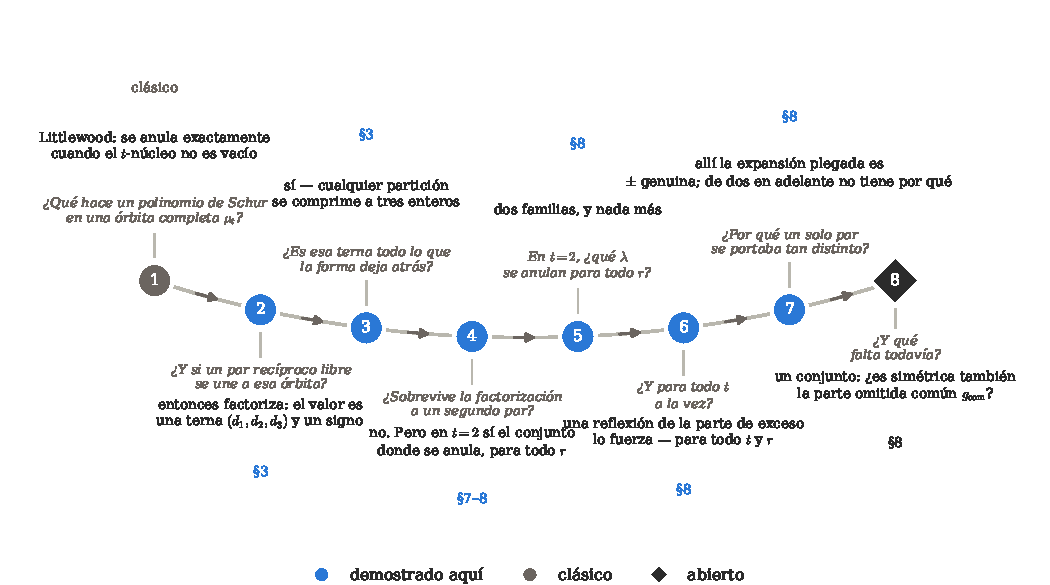
\includegraphics[width=\textwidth]{fig_thread_es.pdf}
\caption{El artículo como un solo hilo. Cada pregunta la responde la perla que tiene debajo, y
cada respuesta es lo que hace que la siguiente pregunta sea la natural: la órbita pide el par
libre, la factorización pide la terna, la terna pide el segundo par, y el segundo par convierte una
fórmula en un lugar. El color distingue lo clásico, lo demostrado aquí y lo que queda abierto, y la
etiqueta bajo cada respuesta es la sección que la resuelve. Dibujada por
\texttt{anc/fig\_intro.py}.}
\label{fig:thread}
\end{figure}

\begin{figure}[!ht]
\centering
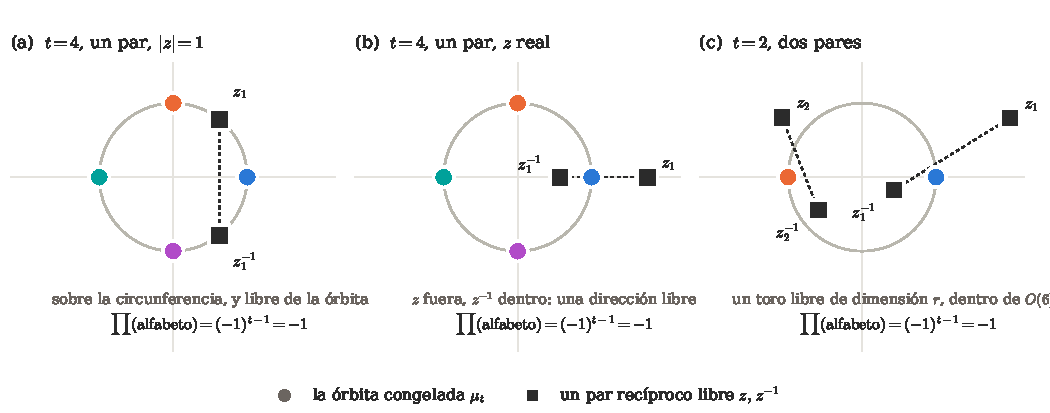
\includegraphics[width=\textwidth]{fig_alphabet_es.pdf}
\caption{El alfabeto, en el plano complejo. La órbita $\mu_t$ está congelada ---un $t$-gono
regular sobre la circunferencia unidad, coloreado por residuo--- y cada par recíproco es una
dirección compleja libre, dibujada unida por un segmento discontinuo. \emph{(a)} el par puede estar
sobre la circunferencia; es una variable libre y no parte de la órbita, y salvo para finitos $z$ no
toca $\mu_t$, que es la razón de que un operador hecho para órbitas de $\zeta$ no tenga nada que
decir de él. \emph{(b)} fuera de la circunferencia, $z$ por fuera y $z^{-1}$ por dentro. \emph{(c)}
$r$ pares dan un toro libre de dimensión $r$. En todos los casos el alfabeto es cerrado por
inversión, así que es la lista de valores propios de un elemento de $O(N,\CC)$ ---el panel (b)
muestra por qué el grupo tiene que ser el complejo--- y el producto de sus letras vale $\zeta^{t(t-1)/2}=(-1)^{t-1}$: para $t$ par esa matriz
está en la componente no identidad. Calculada por \texttt{anc/fig\_intro.py}.}
\label{fig:alphabet}
\end{figure}


Una partición puede ser arbitrariamente grande, y un alfabeto de $N=t+2$ letras sólo alcanza a ver
una parte de ella. Este artículo resuelve, para un alfabeto, exactamente cuánta. El conjunto
completo de las raíces $t$-ésimas de la unidad junto con un par recíproco libre ve un multiconjunto
de tres enteros y un signo, y nada más en absoluto: dos particiones de cualesquiera tamaños que
coincidan en ese dato toman ahí el mismo valor. La forma cerrada del Teorema \ref{thm:main} es cómo
lo demostramos, y la compresión es la parte que esperamos que sobreviva a la fórmula.

La evaluación de polinomios de Schur en raíces de la unidad es clásica y notablemente limpia.
Littlewood y Richardson \cite{LR34} demostraron que $s_\lambda$ se especializa a $0$ o $\pm1$ cuando
las variables se toman como todas las raíces $t$-ésimas de la unidad, siendo el signo un signo de
ordenación y estando la anulación gobernada por el $t$-núcleo de $\lambda$; y en el mismo trabajo lo
generalizaron a un alfabeto que lleva una variable libre en cada letra. Este último resultado fue
redescubierto por Prasad \cite{Pra16}, recibió una nueva demostración de Karmakar \cite{Kar22}, fue
extendido a todos los grupos clásicos por Ayyer y Kumari \cite{AK22} ---quienes además identificaron
el trabajo anterior, casi inadvertido, de Lecouvey \cite{Lec09}--- y fue llevado a los caracteres
universales por Albion \cite{Alb23}. Kumari \cite{Kum24} amplió la familia, Karmakar \cite{Kar24}
trató los elementos de orden dos, Ayyer y Kumari \cite{AK25} añadieron varias especializaciones más,
y Albion \cite{Alb25} relacionó las factorizaciones con las particiones $z$-asimétricas y el
plethysm. Sathish Kumar \cite{SK23} llevó la factorización a las formas sesgadas con
banderas, donde produce una familia de caracteres de Demazure; allí se exige que las banderas
sean múltiplos de $t$, que es la misma demanda de estructura de raíces de la unidad con otro
disfraz. Leída en conjunto, esa línea hace algo más que acumular casos. El enunciado migra de un
grupo a un alfabeto: una vez que los caracteres son universales, evaluar uno es una pregunta sobre
qué letras se escriben, y los tipos clásicos dejan de ser teoremas separados ---el Teorema 5.3 de
\cite{AK25} es un solo enunciado para $s$, $sp$ y $o$ a la vez---. Esa migración es lo que vuelve
formulable la pregunta de este artículo, porque el alfabeto de abajo no pertenece a ningún grupo de
la lista; y las herramientas que tomamos prestadas en la \S\ref{sec:zeros} son las que esa migración
produjo. Remitimos a Albion \cite{Alb23} para un recorrido de toda la línea.

Leído por su \emph{valor}, el teorema de Littlewood es una factorización. Leído por sus \emph{ceros}
es otra cosa ---una clasificación de las $\lambda$ que mueren en un elemento de orden $t$--- y esa
segunda lectura tiene un descendiente propio, que conviene nombrar aquí porque la
\S\ref{sec:zeros} resulta ser su prima. Prasad \cite[Teorema 2]{Pra16} plantea la pregunta de la
anulación no en un punto sino a lo largo de toda una familia: sobre la componente no identidad de
$GL_m^n\rtimes\ZZ/n$ determina cuándo el carácter es idénticamente cero \emph{como función del
parámetro libre}, y la respuesta se lee otra vez en las clases de residuos de $\lambda+\delta$
---cada clase tiene que estar representada exactamente $m$ veces---. En $m=1$ eso es la condición de
Littlewood. Así que un teorema de 1934 tiene dos descendientes, y se separan en qué se permite
que siga libre: allí, órbitas completas de raíces de la unidad; aquí, como veremos, una sola órbita
congelada junto con direcciones \emph{recíprocas} libres. Ninguno de los dos enunciados contiene al
otro.

Una segunda línea de resultados de factorización trata alfabetos cerrados bajo $x\mapsto x^{-1}$.
Okada \cite{Oka98} y Ciucu--Krattenthaler \cite{CK09} trataron las formas rectangulares; Behrend,
Fischer y Konvalinka, y Ayyer, Behrend y Fischer, las escaleras dobles ---para las que seguimos las
atribuciones que da \cite{AB19}---; y Ayyer--Behrend \cite{AB19} las formas autoduales, con
demostraciones biyectivas de estas últimas debidas a Ayyer y Fischer \cite{AF20}. Allí el rédito es
enumerativo: las factorizaciones producen fórmulas de producto para clases de simetría de particiones
planas y para teselaciones de rombos. Las formas autocomplementarias de \cite{AB19} reaparecen en la
\S\ref{sec:zeros} por el otro lado: añadir la letra $-1$ cambia el determinante del alfabeto de $+1$
a $-1$, y las formas que allí factorizan son exactamente las que aquí se anulan.

Las dos líneas nunca han compartido alfabeto, y el obstáculo es estructural en ambas direcciones. El
motor de la primera es un operador ---la Verschiebung $\varphi_t$, en la formulación de Albion
\cite{Alb23}, que actúa sobre los caracteres universales por $\varphi_t h_r=h_{r/t}$ si $t\mid r$ y
$0$ en otro caso--- que exige que el alfabeto sea unión de $\zeta$-órbitas; toda extensión de esa
línea añade por tanto \emph{más} estructura de raíces de la unidad, nunca menos. El motor de la
segunda exige que el alfabeto sea enteramente recíproco, o que la forma sea autocomplementaria. Un
par recíproco libre no es una $\zeta$-órbita, y una órbita de raíces de la unidad no es unión de
pares libres.

La palabra \emph{más pequeño} de abajo puede precisarse, y es el cierre por inversión quien lo
permite. Una extensión de $\zt$ cerrada por inversión solo puede adjuntar pares recíprocos
$\{x,x^{-1}\}$ y los puntos fijos de la inversión, que son $1$ y $-1$; ahora bien, $1$ está en $\zt$
para todo $t$, y $-1$ está en $\zt$ exactamente cuando $t$ es par. La única extensión menor que un
par es por tanto $\zt\cup\{-1\}$ con $t$ impar, y está congelada: sobre $t=3,5,7$ y
$|\lambda|\le14$, las $1092$ formas, $s_\lambda(\zt,-1)$ solo toma los valores $0$ y $\pm1$, sin
nada de lo que pueda depender. Un par recíproco libre es la extensión más pequeña que deja algo que
evaluar.

En este artículo tomamos el alfabeto más pequeño que contiene una letra de cada clase,
\begin{equation}\label{eq:object}
\Phi_t(\lambda;z)\;:=\;s_\lambda\bigl(\,\underbrace{1,\zeta,\dots,\zeta^{t-1}}_{\zt},\;z,\;z^{-1}\bigr),
\qquad \zeta=e^{2\pi i/t},
\end{equation}
un polinomio de Schur en $N=t+2$ variables.

Descrito así, \eqref{eq:object} es un compromiso entre dos líneas, que es como lo encontramos. Se
describe mejor como un solo objeto, y esa descripción es la que reaparece en cada sección de abajo:
\eqref{eq:object} es \emph{un elemento del toro de $O(N)$ con una única dirección libre}. Es cerrado
por inversión, de modo que ya vive donde vive la segunda línea; su determinante es $(-1)^{t+1}$, y
ese determinante es lo que separa factorizar de anularse en la \S\ref{sec:zeros}; la $\zeta$-órbita
es lo que lo coloca en la componente no identidad cuando $t$ es par, donde un carácter es un carácter
entrelazado, que es la Observación \ref{rem:twining}; y el único par libre es la única variable que
sobrevive a la enumeración con signo de la \S\ref{sec:enum}. Los tres resultados de este artículo son
tres lecturas de esa frase.

Nuestro resultado principal, el Teorema \ref{thm:main},
lo evalúa para todo $t$ y toda $\lambda\in\PP_N$ ---toda partición con a lo sumo $N$ partes, sin
restricción alguna sobre su forma ni su tamaño---. Escribimos $\beta=\beta(\lambda,N)$ para la partición
desplazada y $n_i(\lambda)$ para el número de partes de $\beta$ congruentes con $i$ módulo $t$, como
en \cite{AK22}. Puesto que hay $t$ clases de residuos y $N=t+2$ partes, $\sum_i(n_i-1)=2$; luego o
alguna clase está vacía, o, estando todas ocupadas, el exceso sobre una cada una es exactamente dos,
y solo se dan tres perfiles: algún $n_i$ se anula, o dos clases tienen tamaño dos, o una clase tiene
tamaño tres. En el primer caso $\Phi_t=0$; en los otros dos, si $A=\{a_1>a_2\}$ y $B=\{b_1>b_2\}$
denotan las dos clases distinguidas y
\[
d_1=a_1-a_2,\qquad d_2=b_1-b_2,\qquad
\tilde d_3=a_1+a_2-b_1-b_2,\qquad d_3=|\tilde d_3| ,
\]
entonces $\Phi_t=0$ si el \emph{acoplamiento orientado} $\tilde d_3$ se anula, y en otro caso, con
$z=e^{\theta}$,
\[
\boxed{\;\;\Phi_t(\lambda;z)\;=\;\varepsilon_\lambda\,
\frac{\sinh(d_1\theta/2)\,\sinh(d_2\theta/2)\,\sinh(d_3\theta/2)}
{\sinh^2(t\theta/2)\,\sinh\theta}\;\;}
\]
con $\varepsilon_\lambda=\pm1$ dado explícitamente. \emph{Tres factores, nunca más, y sin ninguna
hipótesis sobre la forma de $\lambda$.} Retirado el par recíproco, el enunciado degenera en el de
Littlewood, de modo que el contenido es lo que ese par añade: exactamente un término de
acoplamiento, a saber $d_3$. Leído con caracteres $\mathfrak{sl}_2$ el mismo enunciado no lleva
exponencial ninguna: es el producto triple $\chi_{d_1/2-1}\chi_{d_2/2-1}\chi_{d_3/2-1}$ sobre
$\chi_{t/2-1}^2$, uniformemente en $t$ (Corolario \ref{cor:chars}), con índices semienteros
exactamente cuando $t$ es impar.

El alfabeto es un solo objeto, y la respuesta también. El perfil de residuos, la terna
$(d_1,d_2,d_3)$ y el signo son todo lo que el teorema necesita, y en la \S\ref{sec:main} los
reunimos en un único \emph{invariante de la evaluación} $I_t(\lambda)$, \eqref{eq:invariant}, a
través del cual el valor factoriza. Es completo pero no mínimo: \eqref{eq:main} es simétrica en los
tres enteros, de modo que lo que se ve es el multiconjunto y el signo, que es la compresión
anunciada arriba. Lo que \emph{no} se ve es entonces una pregunta bien planteada. La
\S\ref{sec:fibrelattice} la responde para los tres enteros ---las particiones que los comparten
forman un retículo, y escribimos su función generatriz--- y lo que el signo añade a eso es el
Problema \ref{prob:fibres}.

Los tres enteros admiten una lectura que vuelve transparente la fórmula, y la damos aquí porque es
como pensamos el resultado. Considérense $A$ y $B$ como intervalos $[a_2,a_1]$ y $[b_2,b_1]$ sobre la
recta beta. Entonces
\begin{equation}\label{eq:intervals}
d_1=|A|,\qquad d_2=|B|,\qquad d_3=2\,\bigl|\mathrm{centro}(A)-\mathrm{centro}(B)\bigr| :
\end{equation}
\emph{las dos longitudes, y el doble de la distancia entre los centros} (Figura
\ref{fig:intervals}). El criterio de anulación se vuelve geométrico ---una clase de residuos es
vacía, o los dos intervalos son concéntricos--- y explica de inmediato por qué el perfil de tamaño
tres, donde los intervalos comparten un extremo, nunca se anula. Los intervalos concéntricos
resultan exigir $t$ par (Proposición \ref{rem:lattice}), de modo que para $t$ impar una clase de
residuos vacía es la única forma de anularse ---y eso sigue siendo cierto para cualquier número de
pares recíprocos, que es el Corolario \ref{cor:oddgen}---. Equivalentemente, en el idioma de la
primera línea, $d_1$ y $d_2$ son $t$ veces los contenidos $\mathfrak{sl}_2$ de las dos componentes
distinguidas del cociente, y el acoplamiento orientado $\tilde d_3$ es un funcional \emph{afín} sobre
el vector de \emph{tamaños} del cociente, entrando los dos residuos como un desplazamiento, con
$d_3=|\tilde d_3|$ (Proposición \ref{prop:quotient}). No es
un funcional sobre el vector de residuos, y por tanto tampoco sobre el retículo de raíces de tipo
$A_{t-1}$ bajo la correspondencia de Garvan--Kim--Stanton \cite{GKS90}: ya en $t=2$ el único perfil
de dos clases lleva diez valores distintos de $d_3$ sobre $|\lambda|\le16$. En qué mitad de la
descomposición núcleo--cociente vive cada cláusula del criterio de anulación queda resuelto en la
Proposición \ref{rem:lattice}.

Se siguen dos consecuencias. El Teorema 5.3 de \cite{AK25} determina cuándo un carácter universal es
independiente de las variables por las que se le tuerce, uniformemente en los tres tipos clásicos, y
leído sobre \eqref{eq:object} diría que
$s_\lambda(z,z^{-1},\zt)=s_\lambda(z,z^{-1})$ exactamente sobre los $t$-núcleos, para
$\ell(\lambda)\le2$. Ese criterio está enunciado para variables libres, y un par recíproco no lo es;
sobre ese lugar aparece una familia más, y el Teorema \ref{thm:extra} la clasifica por su núcleo y su cociente. En
\S\ref{sec:enum} leemos la identidad como una enumeración: una fórmula de producto para un recuento
de tablas semiestándar pesado por raíces de la unidad en el que el parámetro $z$ sigue libre, y en
$t=2$ una $(-1)$-enumeración de particiones planas en una caja refinada por $z$.

Las dos últimas secciones hacen una pregunta distinta, no sobre lo que la identidad da sino sobre
hasta dónde alcanza. La \S\ref{sec:sharp} prueba cuatro deformaciones naturales del alfabeto, cada
una de las cuales destruye la identidad, y una sola lectura de la demostración explica las
cuatro. Luego la
\S\ref{sec:zeros} aísla lo que sí sobrevive. Añadir más pares recíprocos cuesta la fórmula de
producto del Teorema \ref{thm:main}, pero
no el \emph{lugar de anulación}: para todo número $r$ de pares, el carácter
$s_\lambda(1,-1,z_1,\bar z_1,\dots,z_r,\bar z_r)$ se anula exactamente cuando el conjunto beta tiene
paridad constante o $\lambda$ es autocomplementaria de anchura impar (Teorema \ref{conj:crit}).
Leído sobre el grupo y no sobre el alfabeto, el mismo enunciado es una clasificación: ésas son
exactamente las $\lambda$ cuyo $GL(N)$-módulo restringe a $O(N)$ de forma estable bajo el giro por
$\det$ (Corolario \ref{cor:dettwist}). Las formas son las autocomplementarias de \cite{AB19}, donde el mismo
alfabeto sin la letra $-1$ hace que el carácter factorice en lugar de anularse; el determinante del
alfabeto decide cuál de las dos cosas pasa. La dirección suficiente es un corolario corto de la
complementación y lo decimos así; el contenido es el recíproco, que demostramos para todo $r$ y toda
$\lambda$, módulo un teorema de rigidez para productos de polinomios de Schur.

Conviene dibujar el mapa, y la Figura \ref{fig:plane} lo es. Adjuntar $r$ pares recíprocos a la
órbita $\zt$ da una familia en los dos parámetros $(t,r)$, y el lugar de anulación está resuelto en
tres partes de ella --- una fila, una columna, y todas las columnas impares, que son medio plano.

\begin{figure}[!ht]
\centering
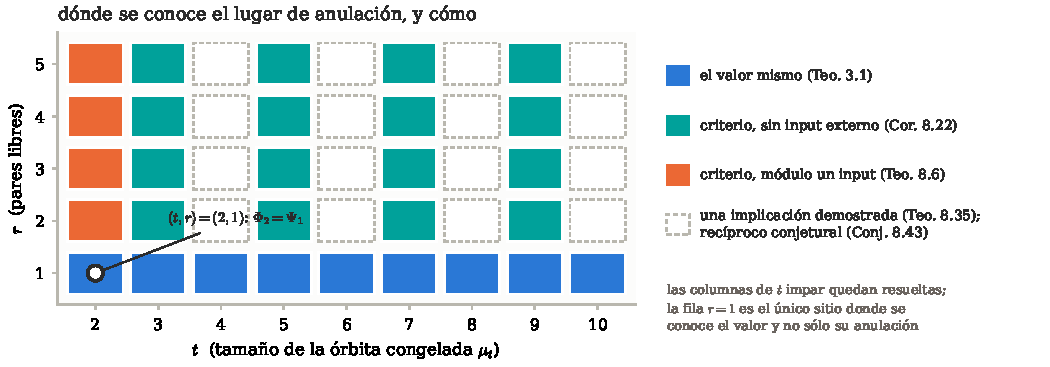
\includegraphics[width=\textwidth]{fig_plane_es.pdf}
\caption{La familia de dos parámetros, y lo que se sabe sobre ella. Cada celda es un alfabeto
$\zt\cup\{z_1^{\pm1},\dots,z_r^{\pm1}\}$; el color no se asigna a mano, sino que se calcula a partir
de los propios enunciados, con una regla por línea del artículo. La fila $r=1$ es el único sitio
donde se conoce el \emph{valor} y no sólo su anulación, que es el Teorema \ref{thm:main}; las
columnas de $t$ impar las resuelve el Corolario \ref{cor:oddgen} sin ningún input externo; la columna
$t=2$, el Teorema \ref{conj:crit}, que usa uno. En las celdas restantes el Teorema \ref{thm:suff}
prueba una implicación y la Conjetura \ref{conj:general} es la otra. La esquina marcada es donde se
encuentran las dos mitades del artículo: allí $\Phi_2=\Psi_1$, y es el único alfabeto que ven las
dos. Calculada por \texttt{anc/fig\_plane.py}.}
\label{fig:plane}
\end{figure} El Teorema \ref{thm:main}
es $r=1$: un par, todo $t$, y ahí tenemos el valor y no sólo su anulación.
El Teorema \ref{conj:crit} es $t=2$: cualquier número de pares, la órbita más pequeña. Y el Corolario
\ref{cor:oddgen} es \emph{todo $t$ impar y todo $r$} a la vez: allí el carácter se anula si y sólo si
falta una clase de residuos, de modo que la rama concéntrica es un fenómeno exclusivo de $t$ par. La
tercera de las tres no es un borde sino medio plano, y es además la más barata --- sale del argumento
extremal de la \S\ref{sec:extremal} sin ningún input externo, mientras que la segunda necesita el
Teorema \ref{thm:PvW}. Fuera de esas tres regiones el lugar no está resuelto, pero ya no está intacto. El
Teorema \ref{thm:suff} da una condición sobre el conjunto beta --- una reflexión de su parte de
exceso, y un incremento que da en el centro --- que fuerza la anulación del carácter para
\emph{todo} $t$ y todo $r$, mediante una involución que empareja todos los términos del desarrollo;
el Corolario \ref{cor:necgen} da una condición necesaria por el otro lado. Que las dos se encuentren
es la Conjetura \ref{conj:general}, y lo que las separa es una sola implicación, que la
\S\ref{sec:rigidity} muestra que no puede venir del estrato en el que ese argumento trabaja. El
fórmula de producto del Teorema \ref{thm:main} ya falla en $r=2$, por (D1) ---que no exista tal
fórmula para ningún $r\ge2$ es la Conjetura \ref{conj:rank2}, y no algo que demostremos---, así que
pasada la línea $r=1$ el lugar es lo que podemos ofrecer.

Hay algo que el alfabeto delata y que merece decirse aquí y no de pasada. Tiene una lectura en
teoría de representaciones ---de la clase que \cite{CK09} registran como ausente para sus
factorizaciones, y con ellos \cite{AB19} y \cite{AK25}--- y el mecanismo no es nuestro: el alfabeto
es cerrado por inversión, luego
un elemento del toro de $O(N)$ de determinante $(-1)^{t+1}$, de modo que para $t$ par vive en la
componente no identidad, donde un carácter es un carácter \emph{entrelazado} en el sentido de
Jantzen \cite{Jantzen} y Kumar--Lusztig--Prasad \cite{KLP} y el plegado lo da el álgebra de Lie de
órbitas. La Observación \ref{rem:twining} lo precisa y el Lema \ref{lem:AtoSp} lo concreta ---allí el
álgebra plegada es $C_r$ y el carácter entrelazado es un carácter simpléctico sin más. La
demostración del Teorema \ref{thm:main} no usa nada de eso, y por eso lo enunciamos como lectura y no
como método.

El artículo se organiza como sigue. Fijamos notación y recordamos las dos evaluaciones sobre las que
construimos en la Sección \ref{sec:background}. En la Sección \ref{sec:main} enunciamos el teorema
principal, identificamos sus tres enteros en términos del núcleo y del $t$-cociente, describimos las
particiones que no consiguen separar y registramos el criterio de
anulación y la imagen de la aplicación resultante. La Sección \ref{sec:proof} contiene la
demostración. En la Sección \ref{sec:independence} comparamos el teorema con el criterio de
independencia de \cite{AK25} y determinamos la familia adicional que adquiere en el lugar recíproco.
En la Sección \ref{sec:enum} leemos el teorema como una enumeración y ensamblamos, en $t=2$, la
involución que invierte el signo que esa enumeración pide, y en la Sección
\ref{sec:sharp} probamos cuatro deformaciones del alfabeto, cada una de las cuales destruye la
identidad. La Sección \ref{sec:zeros} determina
el lugar de anulación en $t=2$ para un número arbitrario de pares recíprocos ---y, sin ningún coste
externo, también en todo $t$ impar---, lee ese criterio sobre el grupo como una rigidez frente al
giro por el determinante, y da un criterio suficiente, con recíproco conjetural, para $t$ y $r$
arbitrarios. La Sección \ref{sec:verif} recoge las
comprobaciones numéricas y la Sección \ref{sec:open} los problemas abiertos.

%======================================================================
\section{Preliminares y notación}\label{sec:background}

Seguimos la notación de \cite{AK22,AK25}. Todos los grupos algebraicos son aquí sobre $\CC$; en
particular $O(N)$ significa $O(N,\CC)$, que es lo que da un alfabeto cerrado por $x\mapsto x^{-1}$
cuando se permite a sus letras salir de la circunferencia unidad.

\subsection{Particiones, conjuntos beta, núcleos y cocientes}
Una partición $\lambda=(\lambda_1,\dots,\lambda_n)$ es una sucesión débilmente decreciente de enteros
no negativos; $\PP_n$ denota el conjunto de particiones de longitud a lo sumo $n$, $|\lambda|$ el
tamaño y $\ell(\lambda)$ la longitud. En todo el texto $t\ge2$ es un entero fijo, $\zeta$ una raíz
$t$-ésima primitiva de la unidad, $\zt=\{1,\zeta,\dots,\zeta^{t-1}\}$, y
\[
N:=t+2 .
\]
Para $\lambda\in\PP_N$ el \emph{conjunto beta} es $\beta(\lambda)=(\beta_1,\dots,\beta_N)$ con
$\beta_j=\lambda_j+N-j$, de modo que $\beta_1>\beta_2>\dots>\beta_N\ge0$; indexamos por
\emph{columnas} $j=1,\dots,N$, y observamos que un $\beta$ mayor significa un índice de columna menor.
Para $0\le i\le t-1$ escribimos $n_i(\lambda)$ para el número de partes de $\beta(\lambda)$
congruentes con $i$ módulo $t$, de manera que
\begin{equation}\label{eq:excess}
\sum_{i=0}^{t-1}n_i(\lambda)=N=t+2 .
\end{equation}
Llamamos \emph{perfil de residuos} de $\lambda$ al vector
$\bigl(n_0(\lambda),\dots,n_{t-1}(\lambda)\bigr)$. Por \eqref{eq:excess},
$\sum_i\bigl(n_i(\lambda)-1\bigr)=2$: o alguna clase está vacía, o, estando todas ocupadas, el
exceso sobre una cada una es exactamente dos, y sólo hay dos particiones de dos. De modo que un
perfil es de exactamente uno de tres tipos: \emph{degenerado}, si algún $n_i=0$; \emph{de dos
clases}, si dos entradas valen $2$; o \emph{de tamaño tres}, si una entrada vale $3$. Todo lo que
sigue en este artículo está gobernado por cuál de los tres se da.
Sea $\sigma\in S_N$ la permutación que reordena las partes de $\beta(\lambda)$ agrupándolas por clase
de residuo, con las clases en orden creciente y los valores dentro de cada clase en orden
decreciente; es la permutación de \cite[(2.1)]{AK25}. Escribimos $\core_t(\lambda)$ y
$\quot_t(\lambda)=(\lambda^{(0)},\dots,\lambda^{(t-1)})$ para el $t$-núcleo y el $t$-cociente,
definidos a partir de $\beta(\lambda)$ como en \cite[\S2.1]{AK25}. Por \cite{GKS90}, los $t$-núcleos
están en biyección con los vectores del retículo de raíces de tipo $A_{t-1}$, y los recuentos de
residuos $n_i$ son las coordenadas naturales.

Ponemos $\zb:=z^{-1}$, $z=e^{\theta}$, y abreviamos
\[
f(u):=z^{u}-z^{-u}=2\sinh(u\theta),\qquad
V:=\prod_{0\le k<k'\le t-1}\bigl(\zeta^{k'}-\zeta^{k}\bigr).
\]
Para un conjunto $S$ de columnas, $b_S$ es la palabra de residuos $\beta_j\bmod t$ para $j\in S$
leída en orden creciente de columna, e $\inv(b_S)$ su número de inversiones. Usamos el bialternante
\[
s_\lambda(x_1,\dots,x_N)=\frac{\det\bigl(x_i^{\beta_j}\bigr)_{i,j=1}^N}
{\det\bigl(x_i^{N-j}\bigr)_{i,j=1}^N}.
\]

\subsection{Las dos evaluaciones sobre las que construimos}
Recordamos los dos enunciados entre los que se sitúa el presente resultado. El primero es la
evaluación de Littlewood, en la forma de \cite[Teorema 2.2]{AK25}.

\begin{theorem}[{\cite[Teorema IX]{LR34}}]\label{thm:LR}
Sea $\lambda\in\PP_t$. Entonces
\[
s_\lambda(1,\zeta,\dots,\zeta^{t-1})=
\begin{cases}
(-1)^{\binom{t}{2}}\sgn(\sigma) & \text{si }\core_t(\lambda)=\varnothing,\\
0 & \text{en otro caso.}
\end{cases}
\]
\end{theorem}

El segundo es el criterio de independencia que extendemos, \cite[Teorema 5.3]{AK25}; enunciamos el
caso que necesitamos. Sea $f_\lambda$ un carácter universal de tipo $s$, $sp$ u $o$, sea $Y$ un
conjunto de $m$ variables y sean $x_1,\dots,x_{n-tm}$ libres. Entonces
\begin{equation}\label{eq:AK53}
f_\lambda(x_1,\dots,x_{n-tm},Y,\zeta Y,\dots,\zeta^{t-1}Y)=f_\lambda(x_1,\dots,x_{n-tm})
\quad\Longleftrightarrow\quad \lambda=\core_t(\lambda),
\end{equation}
para $\lambda\in\PP_{n-tm}$. El criterio es uniforme en el tipo ---un solo enunciado para $s$, $sp$ y
$o$ a la vez---, que es lo que lo hace citable aquí: nuestro alfabeto es un alfabeto de $GL$, y lo
que le preguntamos es una cuestión sobre una especialización y no sobre un grupo. Tomando $m=1$,
$Y=(1)$ y $(x_1,x_2)=(z,\zb)$ se obtiene $n=t+2$ y nuestro alfabeto, pero esa sustitución es
justamente donde se abandona la hipótesis de que $x_1,x_2$ sean libres. Así que \eqref{eq:AK53} no se
está aplicando sobre el lugar recíproco; se le está preguntando por él, que es la
\S\ref{sec:independence}.

\begin{remark}\label{rem:notacase}
El enunciado más próximo de la literatura añade dos letras extra, igual que nosotros, de modo que
conviene registrar por qué no contiene \eqref{eq:object}. Kumari \cite[Teorema 2.2]{Kum24} evalúa
$s_\lambda(X,\zeta X,\dots,\zeta^{t-1}X,\,y,\zeta y,\dots,\zeta^{m-1}y)$; con $X=(1)$ y $m=2$ el
bloque añadido es $\{y,\zeta y\}$, mientras que el nuestro es $\{z,z^{-1}\}$. Los dos coinciden solo
cuando $z^{2}=\zeta^{\pm1}$, un conjunto finito de puntos y no una variable libre. Lo mismo vale para
la única variable libre extra de \cite[Teorema 2.7]{AK22} y para el Teorema XI de
Littlewood--Richardson.
\end{remark}

%======================================================================
La Figura \ref{fig:beta} hace todo el diccionario sobre una forma concreta.

\begin{figure}[!ht]
\centering
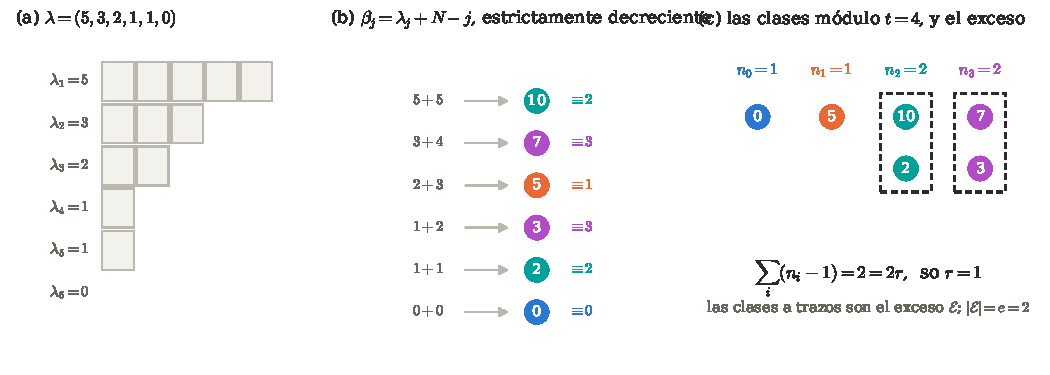
\includegraphics[width=\textwidth]{fig_beta_es.pdf}
\caption{El diccionario sobre el que corre el resto del artículo, con $\lambda=(5,3,2,1,1,0)$ y
$t=4$. \emph{(a)} la forma, rellenada hasta $N$ partes. \emph{(b)} $\beta_j=\lambda_j+N-j$, que
convierte una sucesión débilmente decreciente en una estrictamente decreciente y por tanto en un
conjunto; cada valor se colorea después según su residuo módulo $t$. \emph{(c)} el perfil de
residuos $(n_0,\dots,n_{t-1})$ y el recuento \eqref{eq:excess}: $\sum_i(n_i-1)=2r$ siempre, de modo
que cuando toda clase está ocupada las clases con $n_i\ge2$ ---el exceso $\mathcal{E}$, a trazos---
llevan exactamente $2r$ elementos más de uno cada una. Si alguna está vacía la suma sigue valiendo
$2r$ pero ya no es un exceso: ésa es la rama degenerada, que se resuelve la primera.
Todo lo que el artículo demuestra es un enunciado sobre ese dibujo.
Calculada por \texttt{anc/fig\_intro.py}.}
\label{fig:beta}
\end{figure}

\section{La evaluación}\label{sec:main}

\keybox{\emph{El teorema en una frase.} El valor depende de $\lambda$ a través de su perfil de
residuos, una terna de intervalos $(d_1,d_2,d_3)$ y un signo, y de nada más: una partición
arbitrariamente grande queda comprimida a tres enteros y un signo.}

\begin{theorem}\label{thm:main}
Sean $t\ge2$ y $\lambda\in\PP_N$, con $N=t+2$.
\begin{enumerate}
\item[\rm(i)] Si $n_i(\lambda)=0$ para algún $i$, entonces $\Phi_t(\lambda;z)=0$.
\item[\rm(ii)] En caso contrario, por \eqref{eq:excess}, o bien exactamente dos clases de residuos
tienen $n_i=2$, o bien exactamente una tiene $n_i=3$. Sean $r_A\le r_B$ los residuos implicados y
sean
\[
A=\{a_1>a_2\},\qquad B=\{b_1>b_2\}
\]
en el primer caso las partes de $\beta(\lambda)$ en las clases $r_A$ y $r_B$, y en el segundo los dos
pares solapados $A=\{p,q\}$, $B=\{q,r\}$ de la clase $\{p>q>r\}$, de modo que $r_A=r_B$. Pongamos
\[
d_1=a_1-a_2,\qquad d_2=b_1-b_2,\qquad
\tilde d_3=a_1+a_2-b_1-b_2,\qquad d_3=|\tilde d_3| ,
\]
y llamemos a $\tilde d_3$ el \emph{acoplamiento orientado}. Si $\tilde d_3=0$, entonces
$\Phi_t(\lambda;z)=0$. En caso contrario, con $z=e^\theta$,
\begin{equation}\label{eq:main}
\boxed{\;\;\Phi_t(\lambda;z)\;=\;\varepsilon_\lambda\cdot
\frac{\sinh(d_1\theta/2)\,\sinh(d_2\theta/2)\,\sinh(d_3\theta/2)}
{\sinh^2(t\theta/2)\,\sinh\theta}\;\;}
\end{equation}
donde, escribiendo $j_{A_1}$ y $j_{B_1}$ para las columnas que llevan $a_1$ y $b_1$, $S$ para el
complementario de $\{j_{A_1},j_{B_1}\}$ en $\{1,\dots,N\}$, y $b_S$ para la palabra de residuos de
$\beta(\lambda)$ sobre $S$ leída en orden creciente de columna,
\begin{equation}\label{eq:sign}
\varepsilon_\lambda\;=\;(-1)^{\,t+\binom{N+1}{2}}\;
(-1)^{\,j_{A_1}+j_{B_1}+\inv(b_S)}\;\sgn(a_1-b_1)\;\sgn(\tilde d_3).
\end{equation}
\end{enumerate}
Cada uno de los cuatro factores es $\pm1$ ---el último porque $\tilde d_3\ne0$ es exactamente la
hipótesis de {\rm(ii)}---, luego $\varepsilon_\lambda=\pm1$. En el perfil de tamaño tres $r_A=r_B$ y
$\tilde d_3=p-r>0$, luego ese factor es $+1$.

El lado izquierdo es un polinomio de Laurent en $z$. Leemos \eqref{eq:main} como identidad en
$\CC(z)$; tras la cancelación el lado derecho es también un polinomio de Laurent, y en los ceros del
denominador ---$z=\pm1$ y $z^t=1$--- usamos esa continuación. Así lo hacemos en \S\ref{sec:enum},
donde el valor se toma en $z=1$.
\end{theorem}

\noindent Separar $d_3$ en su tamaño y su orientación no es contabilidad. El signo \eqref{eq:sign}
necesita la orientación y la fórmula necesita solo el tamaño, y en $\tilde d_3=0$ la orientación no
existe: un enunciado que lleve $\sgn(a_1+a_2-b_1-b_2)$ y afirme que vale $\pm1$ es falso sobre el
lugar concéntrico, donde ese argumento es cero. El valor allí es $0$ por el factor
$\sinh(d_3\theta/2)$, de modo que nada de lo que viene después cambia; lo que cambia es que el caso
queda ahora excluido antes de escribir el signo, y no después.

Escribimos
\[
d(\lambda):=(d_1,d_2,d_3)
\]
y lo llamamos la \emph{terna de intervalos} de $\lambda$, siguiendo la lectura
\eqref{eq:intervals}; y llamamos a $d_3$ el \emph{término de acoplamiento}, por ser el único de los
tres que mezcla las dos clases distinguidas.

Conviene dar nombre al dato completo, porque el teorema se lee mejor como un enunciado sobre él que
como una fórmula. Pongamos
\begin{equation}\label{eq:invariant}
\boxed{\;\;I_t(\lambda)\;:=\;\begin{cases}
0 & \text{si el perfil de residuos es degenerado, o }\tilde d_3=0,\\[2pt]
\bigl(d_1,d_2,d_3,\varepsilon_\lambda\bigr) & \text{en otro caso},
\end{cases}\;\;}
\end{equation}
y llamémoslo el \emph{invariante de la evaluación} de $\lambda$. Su primera rama es exactamente el
lugar de anulación del Corolario \ref{cor:zero}, y es una rama y no dos porque en todo él no hay
signo que registrar: \eqref{eq:sign} necesita $\tilde d_3\ne0$. El Teorema \ref{thm:main} dice
entonces dos cosas a la vez. Primera, que $\Phi_t$ \emph{factoriza a través} de $I_t$: la aplicación
$\lambda\mapsto\Phi_t(\lambda;z)$ es la composición de $\lambda\mapsto I_t(\lambda)$ con una función
del invariante solo. Segunda, que ese invariante es \emph{completo} para esta evaluación: si dos
particiones tienen el mismo $I_t$ tienen el mismo $\Phi_t$, sean del tamaño que sean. La completitud
es lo que hace que la compresión anunciada más arriba merezca un nombre y no solo una observación
---dice que el invariante no es un resumen cómodo de la dependencia, sino la dependencia entera--- y
convierte la pregunta natural siguiente, qué olvida el invariante, en una pregunta bien planteada.
La Proposición \ref{prop:minimal} cierra la pregunta por el otro lado: una vez leída la terna como
multiconjunto, tampoco puede suprimirse nada de $I_t$. Así que la \S\ref{sec:fibrelattice} resuelve
qué se olvida para la terna y el Problema \ref{prob:fibres} es lo que deja
el signo. Los $(d_1,d_2,d_3)$ de la Figura \ref{fig:image} son
los valores que toma este invariante, dibujados.

Esa factorización es una sola tubería, y cada flecha pierde información que ya no vuelve:
% multline y no \[...\]: la cadena entera no cabe en una caja de 436 pt, y una formula sin puntos
% de corte no se parte sola.  El corte va tras el paso que pierde los intervalos, que es donde el
% lector para de todos modos.
\begin{multline*}
\lambda\;\longrightarrow\;\beta(\lambda)\;\longrightarrow\;
\bigl(\text{perfil de residuos},\ \text{los dos intervalos distinguidos}\bigr)\\
\longrightarrow\;\bigl(d_1,d_2,d_3,\varepsilon_\lambda\bigr)\;\longrightarrow\;\Phi_t(\lambda;z).
\end{multline*}
Los intervalos hay que llevarlos junto al perfil: el perfil dice qué clases son las distinguidas y
nada sobre dónde caen sus números beta, de modo que no determina la terna.
Coordenada a coordenada, el invariante reparte el trabajo así.

\begin{center}\small
\begin{tabular}{ll}
\toprule
dato de $\lambda$ & qué controla\\
\midrule
perfil de residuos & la rama degenerada de anulación\\
las dos longitudes $d_1,d_2$ & los dos primeros factores\\
la distancia entre los centros, $d_3$ & el factor de acoplamiento, y la rama concéntrica de anulación\\
la orientación $\sgn(\tilde d_3)$ & un factor del signo\\
el signo de ordenación $\varepsilon_\lambda$ & el signo global\\
\bottomrule
\end{tabular}
\end{center}

\noindent Ninguna de las dos ramas de anulación es la otra: el perfil no puede ver la concéntrica, y
la terna no puede ver la degenerada, y por eso el criterio del Corolario \ref{cor:zero} tiene dos
cláusulas y la \S\ref{sec:main} dedica una proposición a decir dónde vive cada una.

\keybox{Un solo recuento recorre el artículo. Con $t$ clases de residuos, $N=t+2$ partes y toda
clase ocupada, el exceso es exactamente dos, de modo que por \eqref{eq:excess} un perfil sólo
puede ser degenerado, de dos
clases o de tamaño tres: esa tricotomía es la forma del Teorema \ref{thm:main}, la
división en casos de su demostración en la \S\ref{sec:proof}, y la primera rama del lugar de
anulación en la \S\ref{sec:zeros}. Dos clases distinguidas son lo que el par recíproco tiene que
acoplar, y de ahí exactamente un término de acoplamiento y tres factores en vez de dos.}

El recuento de tres tiene una segunda explicación, que no debe nada a la demostración. El exceso
dos da dos clases distinguidas, que son dos intervalos sobre la recta beta, y un par de intervalos
son cuatro números $(a_1,a_2,b_1,b_2)$. Los tres argumentos de \eqref{eq:main} ven qué forma tiene
ese par y no dónde está: un desplazamiento común $\beta\mapsto\beta+m$ deja $d_1$, $d_2$ y
$\tilde d_3$ intactos. Así que lo único que puede entrar en ellos es un funcional lineal que mate la
traslación común, y esos forman el hiperplano $\sum\alpha_i=0$ del dual de dimensión cuatro: un
espacio de dimensión exactamente \emph{tres}. La terna $d_1=(1,-1,0,0)$, $d_2=(0,0,1,-1)$ y
$\tilde d_3=(1,1,-1,-1)$ es una base de él. Módulo la traslación común, un par de intervalos tiene
tres coordenadas lineales independientes, y de ahí sale el recuento de tres. Lo que el Teorema
\ref{thm:main} añade, y que el recuento de dimensiones \emph{no} fuerza, es que en esta
especialización esas tres coordenadas \emph{se separan multiplicativamente}: un producto con un
factor de cada una, y no otra función de tres variables.

El \emph{valor} no es invariante por traslación, y merece la pena decirlo, porque lo que es en su
lugar es una restricción sobre el signo. Un desplazamiento $\beta\mapsto\beta+m$ es
$\lambda\mapsto\lambda+(m^N)$, y $s_{\lambda+(m^N)}(A)=\det(A)^{m}s_\lambda(A)$ para cualquier
alfabeto $A$, así que por \eqref{eq:object}
\begin{equation}\label{eq:shift}
\Phi_t\bigl(\lambda+(m^N);z\bigr)\;=\;(-1)^{(t+1)m}\,\Phi_t(\lambda;z).
\end{equation}
Para $t$ impar el valor es invariante; para $t$ par un desplazamiento impar lo invierte. La terna no
se mueve, de modo que toda esa inversión la lleva $\varepsilon_\lambda$ --- lo que convierte a
\eqref{eq:shift} en una comprobación de \eqref{eq:sign} que no cuesta nada y que el signo supera,
sobre las formas de la \S\ref{sec:verif}. Es además la razón de que el lema haya que enunciarlo sobre
la terna y no sobre el valor: para $t$ par el valor no es función de la clase de traslación de la
terna.

El signo \eqref{eq:sign} es un signo de ordenación, de la misma especie que el del Teorema
\ref{thm:LR}; la Proposición \ref{rem:sign} registra más abajo una expresión más corta para él, en la
notación de \cite{AK25}.

El miembro derecho de \eqref{eq:main} es un cociente, y el contenido del teorema es que ese cociente
es un polinomio de Laurent en $z$. Para $t$ impar el factor $\sinh(t\theta/2)$ por separado no es un
monomio de Laurent, de modo que los tres factores no están individualmente en $\ZZ[z,z^{-1}]$; solo
lo está su combinación. Aun así el enunciado es uniforme en $t$.

\begin{corollary}\label{cor:zero}
$\Phi_t(\lambda;z)\equiv0$ si y solo si alguna clase de residuos módulo $t$ es vacía, o
$a_1+a_2=b_1+b_2$. En particular el perfil de tamaño tres nunca se anula.
\end{corollary}

\noindent La anulación es idéntica en $z$, no en un punto: cuando ocurre, $\lambda$ no aporta nada en
ningún elemento de la familia de un parámetro que barre el par recíproco. Ésa es la forma en que se
planteaba la pregunta de Prasad en la \S\ref{sec:background}, y el sentido en que \eqref{eq:object}
se lee fuera de la combinatoria ---siendo la mitad congelada del alfabeto una holonomía de orden
finito, y el par libre lo que queda del toro---.

\begin{corollary}\label{cor:chars}
Escribamos $\chi_k(z)=(z^{k+1}-z^{-k-1})/(z-z^{-1})$ para el carácter del $\mathfrak{sl}_2$-módulo
irreducible de dimensión $k+1$ cuando $k\ge0$ es entero. Para $k$ semientero conservamos la misma
fórmula, leída en $u=z^{1/2}$; es entonces notación y no un carácter, porque los factores por
separado no son de Laurent en $z$. Entonces
\eqref{eq:main} puede escribirse sin ninguna exponencial y sin convenio alguno para $\theta$:
\begin{equation}\label{eq:chiratio}
\boxed{\;\;\Phi_t(\lambda;z)\;=\;\varepsilon_\lambda\,
\frac{\chi_{\frac{d_1}{2}-1}(z)\;\chi_{\frac{d_2}{2}-1}(z)\;\chi_{\frac{d_3}{2}-1}(z)}
{\chi_{\frac{t}{2}-1}(z)^{2}}\;\;}
\end{equation}
Para $t=2$ el denominador es $\chi_0=1$ y todo $d_i$ es par, luego $\Phi_2$ es sin más un producto
con signo de tres caracteres $\mathfrak{sl}_2$. Para $t$ impar los índices son semienteros, que es el
enunciado de arriba en otra forma: los tres factores no son Laurent por separado, y solo lo es el
cociente. Cada factor se lee en $u=z^{1/2}$ y cambia de signo bajo $u\mapsto-u$ exactamente cuando
su índice es semientero; como $d_1+d_2+d_3$ es par ---tiene la paridad de
$d_1+d_2+\tilde d_3=2(a_1-b_2)$---, el cociente no cambia, y es el polinomio de Laurent en $z$ de
\eqref{eq:main}.
\end{corollary}

\begin{proof}
Escribamos $f(u)=z^{u}-z^{-u}=2\sinh(u\theta)$, de modo que $\chi_k=f(k+1)/f(1)$. El numerador de
\eqref{eq:main} es $f(d_1/2)f(d_2/2)f(d_3/2)/8$ y su denominador es $f(t/2)^2f(1)/8$, así que
\eqref{eq:main} vale $\varepsilon_\lambda f(d_1/2)f(d_2/2)f(d_3/2)/\bigl(f(t/2)^2f(1)\bigr)$;
sacando tres factores $f(1)$ del numerador y dos del denominador se obtiene \eqref{eq:chiratio}.
\end{proof}

\subsection{Los tres enteros vienen del cociente}
Lo siguiente identifica $(d_1,d_2,d_3)$ en el idioma de la línea de raíces de la unidad. Para una
partición $\nu$ ponemos $k(\nu)=\nu_1-\nu_2$, su contenido $\mathfrak{sl}_2$.

\begin{proposition}\label{prop:quotient}
En el perfil de dos clases, con $\quot_t(\lambda)=(\lambda^{(0)},\dots,\lambda^{(t-1)})$,
\[
d_1=t\bigl(k(\lambda^{(r_A)})+1\bigr),\qquad
d_2=t\bigl(k(\lambda^{(r_B)})+1\bigr),\qquad
\tilde d_3=t\bigl(|\lambda^{(r_A)}|-|\lambda^{(r_B)}|\bigr)+2(r_A-r_B) .
\]
En el perfil de tamaño tres la única componente distinguida $\lambda^{(r_A)}$ tiene tres partes y
\[
d_1=t\bigl(\lambda^{(r_A)}_1-\lambda^{(r_A)}_2+1\bigr),\quad
d_2=t\bigl(\lambda^{(r_A)}_2-\lambda^{(r_A)}_3+1\bigr),\quad \tilde d_3=d_1+d_2 .
\]
\end{proposition}

\begin{proof}
Escribamos $a_i=t\tilde a_i+r_A$. La clase $r_A$ lleva dos números beta, luego
$\lambda^{(r_A)}=(\tilde a_1-1,\tilde a_2)$ por la definición del cociente, de donde
$k(\lambda^{(r_A)})=\tilde a_1-\tilde a_2-1$ y $d_1=t(\tilde a_1-\tilde a_2)$, que es la primera
identidad; la segunda es el mismo cálculo. Para la tercera, $\tilde a_1+\tilde a_2=|\lambda^{(r_A)}|+1$
y análogamente para $B$, luego $a_1+a_2-b_1-b_2=t(|\lambda^{(r_A)}|-|\lambda^{(r_B)}|)+2(r_A-r_B)$. El
caso de tamaño tres es idéntico con $\lambda^{(r_A)}=(\tilde p-2,\tilde q-1,\tilde r)$.
\end{proof}

Para $t=2$ la tercera identidad se lee $\tilde d_3=2\bigl(|\lambda^{(0)}|-|\lambda^{(1)}|-1\bigr)$, lo que
ya muestra que $\tilde d_3$ es un funcional sobre los tamaños del cociente y no sobre el vector de
residuos, luego tampoco sobre el retículo de raíces de tipo $A_{t-1}$ bajo la correspondencia de
Garvan--Kim--Stanton \cite{GKS90} entre ese retículo y los $t$-núcleos. La condición $r_B-r_A=t/2$,
que gobierna la familia del Teorema \ref{thm:extra}, es un elemento de orden dos del cociente
correspondiente, y esa es la fuente de los fenómenos de paridad de todo el artículo.

\begin{proposition}[el lugar concéntrico]\label{rem:lattice}
En el perfil de dos clases, ordenado de modo que $r_A<r_B$,
\[
\boxed{\;\;d_3=0\quad\Longleftrightarrow\quad t\ \text{es par},\quad r_B-r_A=\tfrac t2,
\quad\text{y}\quad \bigl|\lambda^{(r_A)}\bigr|=\bigl|\lambda^{(r_B)}\bigr|+1\;\;}
\]
En particular, para $t$ impar $\Phi_t(\lambda;z)=0$ si y solo si alguna clase de residuos módulo $t$
es vacía: allí la cláusula concéntrica del Corolario \ref{cor:zero} es vacua.
\end{proposition}

\begin{proof}
Como $a_1,a_2\equiv r_A$ y $b_1,b_2\equiv r_B$ módulo $t$, la igualdad $a_1+a_2=b_1+b_2$ fuerza
$2r_A\equiv2r_B$, es decir $t\mid2(r_B-r_A)$. Para $t$ impar esto da $t\mid r_B-r_A$ y por tanto
$r_A=r_B$, que es el perfil de tamaño tres, donde $d_3=d_1+d_2>0$ por la Proposición
\ref{prop:quotient}. Para $t$ par y $0\le r_A<r_B\le t-1$ la única solución de $t\mid2(r_B-r_A)$ es
$r_B-r_A=t/2$. Escribiendo $a_1+a_2=t\bigl(|\lambda^{(r_A)}|+1\bigr)+2r_A$ como en la demostración
de la Proposición \ref{prop:quotient}, y análogamente para $B$, la igualdad se convierte en
$t\bigl(|\lambda^{(r_A)}|-|\lambda^{(r_B)}|\bigr)=2(r_B-r_A)=t$.
\end{proof}

Las dos cláusulas del Corolario \ref{cor:zero} viven, pues, en mitades distintas de la
descomposición núcleo--cociente, y esa es la respuesta a la pregunta que el criterio plantea. La
primera es una condición sobre el perfil de residuos, y por tanto sobre el $t$-núcleo: los
hiperplanos coordenados $n_i=0$ recortados sobre la rebanada $\sum_i n_i=t+2$, que no es el arreglo
de Coxeter de tipo $A_{t-1}$. La segunda no es una condición sobre el núcleo en absoluto; es un
único hiperplano en los tamaños del cociente, y los pares de residuos admisibles están indexados por
el elemento de orden dos $r_B-r_A=t/2$ y no por reflexión alguna. No puede existir ninguna
reformulación del criterio de anulación en términos de $\core_t(\lambda)$ solo, que es para $\Phi_t$
lo que la Observación \ref{rem:core} registra para $\Psi_r$.

\subsection{Lo que la terna olvida}\label{sec:fibrelattice}
La Proposición \ref{prop:quotient} lee la terna del cociente. Recorrida al revés, esa misma
lectura dice qué particiones no puede distinguir la terna, y lo dice exactamente. Nada de esto es
profundo ---es la biyección núcleo--cociente a perfil fijo--- pero es lo que convierte la
compresión del Teorema \ref{thm:main} de una imagen en un recuento.

\begin{proposition}[el estrato de dos clases es un retículo]\label{prop:fibrelattice}
Sean $t\ge2$, $N=t+2$, y sea $\mathcal{T}_t\subset\PP_N$ el conjunto de particiones de perfil de dos
clases. Enviar $\lambda$ a sus dos residuos distinguidos junto con su $t$-cociente es una biyección
\begin{equation}\label{eq:fibrelattice}
\mathcal{T}_t\;\xrightarrow{\ \sim\ }\!\!\!\coprod_{0\le r_A<r_B\le t-1}\!\!\!
\PP_2\times\PP_2\times\ZZ_{\ge0}^{\,t-2},
\qquad
\lambda\longmapsto\bigl(r_A,r_B;\ \lambda^{(r_A)},\lambda^{(r_B)};\ (m_i)_{i\ne r_A,r_B}\bigr),
\end{equation}
donde $m_i$ es la única parte de $\lambda^{(i)}$. Bajo ella $\core_t(\lambda)$ depende solo del par
$(r_A,r_B)$; escribimos $\kappa(r_A,r_B)$ para su tamaño. Entonces
\begin{equation}\label{eq:sizelattice}
|\lambda|\;=\;\bigl|\core_t(\lambda)\bigr|
+t\Bigl(\bigl|\lambda^{(r_A)}\bigr|+\bigl|\lambda^{(r_B)}\bigr|+\textstyle\sum_i m_i\Bigr).
\end{equation}
\end{proposition}

\begin{proof}
Una clase que lleva $n_i$ números beta $a_1>\dots>a_{n_i}$, escritos $a_j=t\tilde a_j+i$, aporta
$\lambda^{(i)}=(\tilde a_1-n_i+1,\dots,\tilde a_{n_i})$, de modo que una clase de tamaño $n_i$ da
una partición con a lo sumo $n_i$ partes, y toda partición así proviene de una única
$(\tilde a_j)$ estrictamente decreciente. En el perfil de dos clases los tamaños son $2,2$ y $1$
repetido $t-2$ veces, que es \eqref{eq:fibrelattice}; los residuos se registran en vez de olvidarse
porque el perfil forma parte del dato, y determinan $\core_t(\lambda)$ por la coordenada de
Garvan--Kim--Stanton de la Observación \ref{rem:core}. Entonces \eqref{eq:sizelattice} es la
biyección núcleo--cociente.
\end{proof}

\begin{corollary}[la fibra de la terna, y su función generatriz]\label{cor:fibregf}
Sea $(d_1,d_2,d_3)$ una terna de intervalos alcanzada en el perfil de dos clases, y pongamos
$k_A=d_1/t-1$ y $k_B=d_2/t-1$. Su fibra en $\mathcal{T}_t$ es infinita. Es la unión disjunta de las
ramas indexadas por los pares $r_A<r_B$ y los signos $\eta=\pm1$ para los que
\begin{equation}\label{eq:branch}
c:=\tfrac12\Bigl(\tfrac{\eta\,d_3-2(r_A-r_B)}{t}-k_A+k_B\Bigr)\ \in\ \ZZ ,
\end{equation}
dando los dos signos una única y misma rama cuando $d_3=0$. Sobre una rama los parámetros
libres son un entero $v\ge\max(0,c)$ y $(m_i)\in\ZZ_{\ge0}^{t-2}$, con
$\lambda^{(r_A)}=(v+k_A,v)$ y $\lambda^{(r_B)}=(v-c+k_B,v-c)$. En consecuencia
\begin{equation}\label{eq:fibregf}
\sum_{\lambda\ \mathrm{en\ la\ fibra}}\!\!q^{|\lambda|}
\;=\;\frac{\sum_{\mathrm{ramas}}q^{\,e}}{\bigl(1-q^{4t}\bigr)\bigl(1-q^{t}\bigr)^{t-2}},
\qquad e=\kappa(r_A,r_B)+t\bigl(k_A+k_B-2c\bigr)+4t\max(0,c),
\end{equation}
y el número de $\lambda$ en la fibra con $|\lambda|\le n$ es a la larga un cuasi-polinomio en $n$ de
grado $t-1$ ---a la larga, porque los desplazamientos $q^{\,e}$ del numerador dejan el recuento en
$0$ por debajo del menor de ellos---.
\end{corollary}

\begin{proof}
Por la Proposición \ref{prop:quotient} las dos primeras entradas fijan $k(\lambda^{(r_A)})$ y
$k(\lambda^{(r_B)})$, así que cada componente distinguida queda determinada por su tamaño solo;
escribiéndolas $(v+k_A,v)$ y $(u+k_B,u)$, la tercera entrada dice
$t\bigl((2v+k_A)-(2u+k_B)\bigr)+2(r_A-r_B)=\eta\,d_3$, que es \eqref{eq:branch} con $c=v-u$; el
valor absoluto de $d_3$ es lo que pone ahí los dos signos, y es vacuo en $d_3=0$.
Sustituyendo en \eqref{eq:sizelattice} queda $|\lambda|=e+4t\bigl(v-\max(0,c)\bigr)+t\sum_i m_i$, y
sumar las series geométricas en $v$ y en cada $m_i$ da \eqref{eq:fibregf}. Su denominador tiene
$t-1$ factores, de donde el grado.
\end{proof}

\begin{remark}[el signo no va de pasajero]\label{rem:signsees}
Dos lecturas, y la segunda es una advertencia. Primera: una fibra es infinita para todo $t$ y toda
terna alcanzada, que es lo que muestra la Figura \ref{fig:fibres} y lo que explica
\eqref{eq:fibregf} ---las columnas de ahí no se adelgazan porque una fibra es una sección de
retículo y no un accidente finito. Segunda: \eqref{eq:fibregf} es la fibra de la \emph{terna} y no
la de $I_t$. Las $t-2$ partes $m_i$ son invisibles para $(d_1,d_2,d_3)$ por la Proposición
\ref{prop:quotient}, y sería natural leerlas como direcciones a lo largo de las cuales $\Phi_t$ es
constante. No lo son, desde $t=3$: el signo sí las ve, como \eqref{eq:sign} permite, ya que
$\varepsilon_\lambda$ lleva $\inv(b_S)$, un estadístico de la palabra beta entera, mientras
\eqref{eq:fibrelattice} parte esa palabra en dos clases distinguidas y $t-2$ letras libres. Sobre
los rangos de la \S\ref{sec:verif} el signo es constante en $(m_i)$ a $v$ fijo en los $107$ huecos
de $t=2$, pero solo en $43$ de $62$ en $t=3$ y $26$ de $36$ en $t=4$. Qué hace el signo sobre una
rama es el Problema \ref{prob:fibres}.
\end{remark}

\subsection{La lectura por intervalos}\label{sec:intervals}
La Figura \ref{fig:intervals} dibuja \eqref{eq:intervals} en un ejemplo. El Corolario \ref{cor:zero}
se lee: el carácter se anula cuando una clase de residuos es vacía, o cuando los dos intervalos son
\emph{concéntricos}; y dos intervalos que comparten un extremo son concéntricos solo si coinciden,
por lo que el perfil de tamaño tres nunca se anula.

\begin{figure}[t]
\centering
\begin{tikzpicture}[font=\small,x=1.3cm,y=1.0cm]
\draw[blue!55!black,very thick] (1,1.25) -- (7,1.25);
\draw[blue!55!black,thick] (1,1.10) -- (1,1.40);
\draw[blue!55!black,thick] (7,1.10) -- (7,1.40);
\filldraw[blue!55!black] (4,1.25) circle (1.8pt);
\node[blue!55!black,above=9pt] at (4,1.25) {$A=\{7,1\}$,\quad $d_1=6$};
\draw[red!60!black,very thick] (2,-1.25) -- (5,-1.25);
\draw[red!60!black,thick] (2,-1.40) -- (2,-1.10);
\draw[red!60!black,thick] (5,-1.40) -- (5,-1.10);
\filldraw[red!60!black] (3.5,-1.25) circle (1.8pt);
\node[red!60!black,below=9pt] at (3.5,-1.25) {$B=\{5,2\}$,\quad $d_2=3$};
\draw[->,gray!70] (-0.55,0) -- (8.1,0) node[right,black]{$\beta$};
\foreach \b in {0,...,7} \draw[gray!45] (\b,-0.07) -- (\b,0.07);
\foreach \b in {3,6} \node[gray,font=\scriptsize,below=4pt] at (\b,0) {$\b$};
\foreach \b/\c/\r in {7/blue!55!black/1, 5/red!60!black/2, 2/red!60!black/2,
                      1/blue!55!black/1, 0/gray!55/0}
  {\filldraw[\c] (\b,0) circle (2.7pt);
   \node[\c,font=\scriptsize,below=4pt] at (\b,0) {$\b$};
   \node[\c,font=\scriptsize,above=4pt] at (\b,0) {$\r$};}
\draw[gray!70,dashed] (4,1.25) -- (4,-0.62);
\draw[gray!70,dashed] (3.5,-1.25) -- (3.5,-0.62);
\draw[{Latex[length=1.5mm]}-{Latex[length=1.5mm]},thick] (3.5,-0.62) -- (4,-0.62);
\node[font=\scriptsize,gray!60!black,anchor=west] at (-0.55,1.25) {residuo $1$};
\node[font=\scriptsize,gray!60!black,anchor=west] at (-0.55,-1.25) {residuo $2$};
\end{tikzpicture}
\caption{El mecanismo para $t=3$, $\lambda=(3,2)$: aquí $N=5$, $\beta=(7,5,2,1,0)$ con residuos
$(1,2,2,1,0)$ módulo $3$, de modo que ninguna clase es vacía y dos clases tienen tamaño dos. Los tres
argumentos de \eqref{eq:main} son las dos longitudes de los intervalos y el doble de la distancia
entre sus centros; la flecha doble corta marca esa distancia, aquí $\tfrac12$, de modo que $d_3=1$.}
\label{fig:intervals}
\end{figure}

\begin{example}
Para $t=3$, $\lambda=(3,2)$ como en la Figura \ref{fig:intervals}, $(d_1,d_2,d_3)=(6,3,1)$ y
\[
\Phi_3\bigl((3,2);z\bigr)=\varepsilon\,
\frac{\sinh(3\theta)\sinh(\theta/2)}{\sinh(3\theta/2)\sinh\theta}.
\]
Para $t=3$, $\lambda=(3,1)$ el perfil es el de tamaño tres, $(d_1,d_2,d_3)=(3,3,6)$ y
$\Phi_3=\varepsilon\,\chi_2(z)$. Para $t=4$, $\lambda=(1,1,1)$ se tiene $\beta=(6,5,4,2,1,0)$, la
clase $3$ es vacía y $\Phi_4=0$.
\end{example}

\subsection{La imagen de la aplicación}
El Teorema \ref{thm:main} envía toda partición con a lo sumo $N$ filas a tres enteros, de modo que
toda la familia colapsa sobre un subconjunto disperso de $\ZZ^3$. Por la Proposición
\ref{prop:quotient} las dos primeras coordenadas son múltiplos de $t$; la tercera no lo es, salvo en
el perfil de tamaño tres, donde $d_3=d_1+d_2$. La Figura \ref{fig:image} muestra la imagen para $t=3$
y $t=4$, coloreada por el número de particiones que colapsan en cada punto.

\begin{figure}[t]
\centering
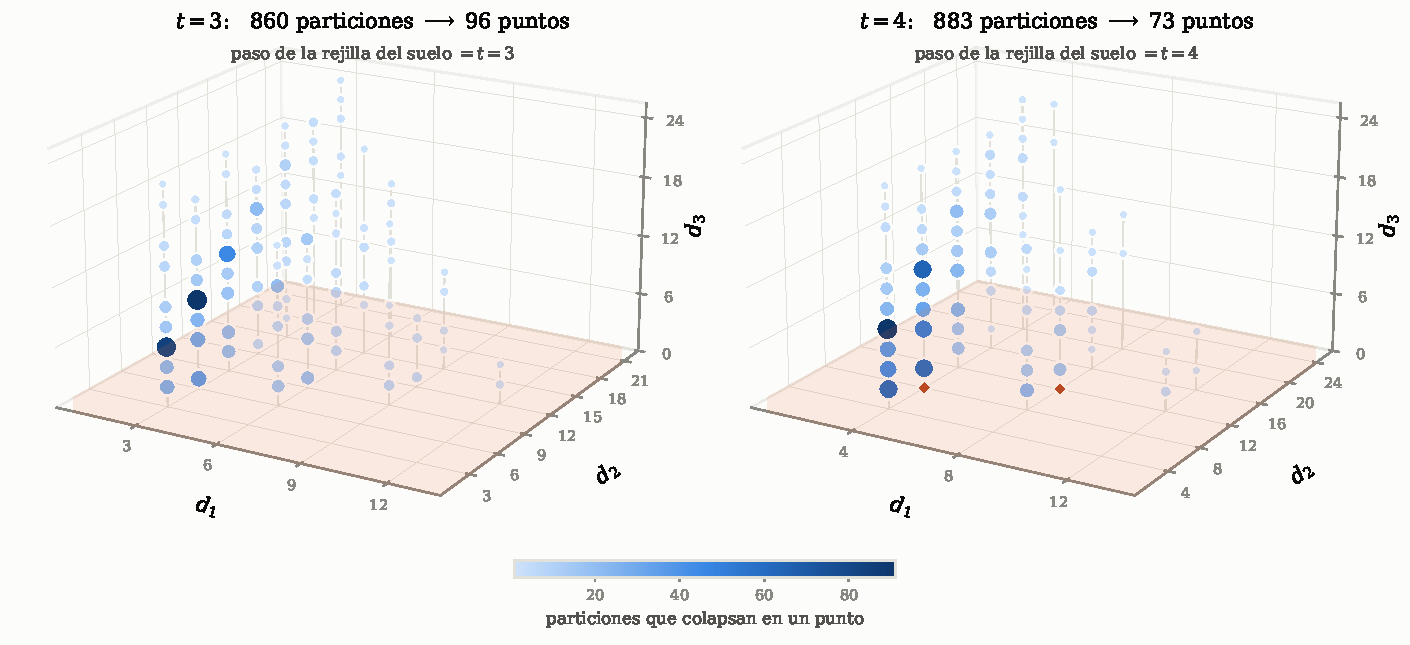
\includegraphics[width=\textwidth]{fig_image_es.pdf}
\caption{La imagen de $\lambda\mapsto(d_1,d_2,d_3)$ sobre todas las $\lambda$ con $|\lambda|\le20$ y
a lo sumo $t+2$ filas, para $t=3$ (izquierda) y $t=4$ (derecha), tomada \emph{salvo el intercambio de
$d_1$ y $d_2$}, bajo el cual \eqref{eq:main} es simétrica; sin esa identificación, y con $A$ y $B$ en
el orden $r_A\le r_B$ del Teorema \ref{thm:main}, los dos paneles llevan $126$ y $92$ puntos en vez
de $96$ y $73$. La compresión es el asunto de la figura: $860$
particiones aterrizan sobre $96$ ternas a la izquierda y $883$ sobre $73$ a la derecha, y el color y
el área dan el número de particiones que va a parar a cada una. El paso de la rejilla del suelo es $t$, pues
$d_1,d_2\in t\ZZ$ por la Proposición \ref{prop:quotient}; el plano sombreado $d_3=0$ es el lugar
concéntrico del Corolario \ref{cor:zero}, donde $s_\lambda$ se anula, así que esas formas no están
en la imagen y se dibujan sobre el plano como rombos. Los dos paneles son las dos paridades, que es
el contenido de la Proposición \ref{rem:lattice}: el impar no lleva ningún rombo, y no puede
llevarlo; el par lleva dos, que son entre ambos la imagen de $32$ particiones.}
\label{fig:image}
\end{figure}

La Figura \ref{fig:image} es una mitad de la imagen: muestra qué ternas se dan, no qué esconde una
terna. La Figura \ref{fig:fibres} es la otra mitad. Sobre cada celda del suelo $(d_1,d_2)$ se levanta
la columna de los tamaños $|\lambda|$ que aterrizan ahí, de modo que una columna es un conjunto de
particiones de tamaños distintos sobre las que $\Phi_t$ toma un único y mismo valor ---y las columnas
no se adelgazan al crecer $|\lambda|$, porque los valores están confinados a un retículo y las
particiones no. La más visible es la fibra de la partición vacía: en $t=3$ el invariante
$I_3=(3,3,2,+1)$ lo comparten $26$ particiones, de $19$ tamaños distintos entre $0$ y $20$, así que
$\Phi_3$ no distingue $\varnothing$ de una forma de veinte cajas.

\begin{figure}[!ht]
\centering
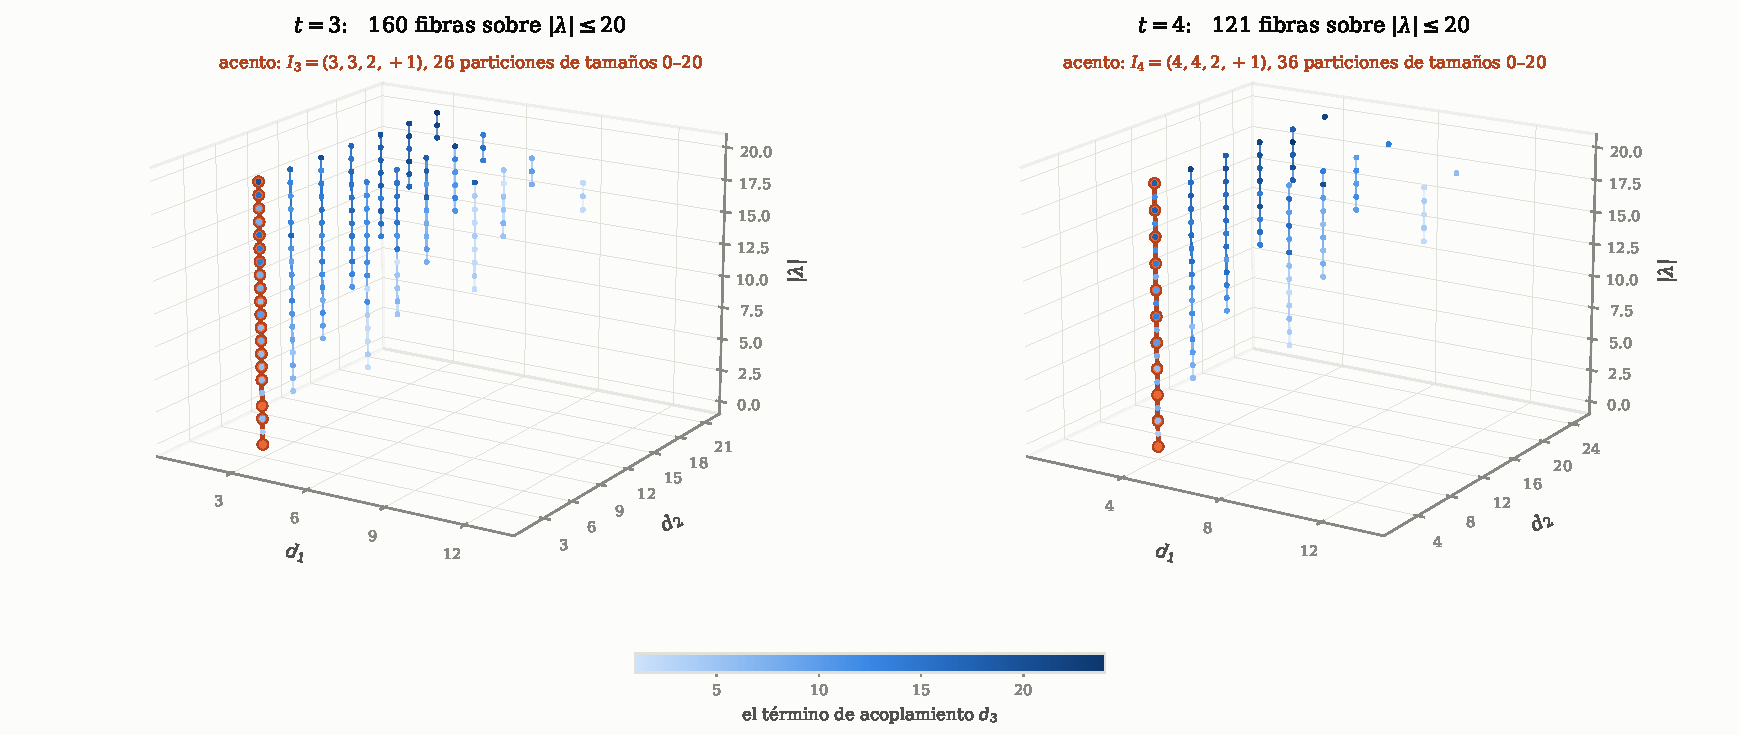
\includegraphics[width=\textwidth]{fig_fibres_es.pdf}
\caption{Las fibras del invariante de la evaluación \eqref{eq:invariant}, complemento de la Figura
\ref{fig:image}: el mismo rango $|\lambda|\le20$, con el término de acoplamiento pasado al color y el
tamaño $|\lambda|$ en el eje vertical. Una columna es una fibra, así que su altura es el rango de
tamaños que este alfabeto no sabe separar; las marcas del suelo son el retículo $t\ZZ$ de la
Proposición \ref{prop:quotient}, y solo está ocupada la mitad $d_1\le d_2$ porque la terna se toma
salvo el intercambio, como en la Figura \ref{fig:image}. Que todas las marcas de una columna lleven
el mismo valor está computado, no supuesto: sobre las $860$ particiones de la izquierda y las $883$
de la derecha el bialternante es constante en cada fibra hasta $10^{-37}$. La columna en color de
acento es la fibra de $\lambda=\varnothing$.}
\label{fig:fibres}
\end{figure}

La Figura 
\ref{fig:fibres} precisa una cosa sobre \eqref{eq:invariant}: $I_t$ es completo pero no mínimo.
El numerador de \eqref{eq:main} es simétrico en $d_1,d_2,d_3$, de modo que el valor solo ve el multiconjunto
$\{d_1,d_2,d_3\}$ junto con el signo, y esa es una reducción real ---sobre $t=4$ y $|\lambda|\le20$
los $121$ invariantes toman solo $110$ valores, mientras que en $t=3$ y el mismo rango los dos
recuentos coinciden. Esa reducción es toda la que hay: por debajo del multiconjunto y del signo no se
pierde nada, y es aquí donde la compresión anunciada en la introducción se vuelve un enunciado exacto
en vez de una cota superior.

\begin{proposition}[el multiconjunto y el signo son exactamente lo que se ve]\label{prop:minimal}
Fíjese $t\ge2$ y sean $\lambda,\mu\in\PP_N$ con $\Phi_t(\lambda;z)\not\equiv0$. Entonces
\[
\Phi_t(\lambda;z)=\Phi_t(\mu;z)
\quad\Longleftrightarrow\quad
\{d_1,d_2,d_3\}(\lambda)=\{d_1,d_2,d_3\}(\mu)\ \text{como multiconjuntos y}\
\varepsilon_\lambda=\varepsilon_\mu .
\]
\end{proposition}

\begin{proof}
$(\Leftarrow)$ es \eqref{eq:main}, cuyo miembro derecho es simétrico en los tres argumentos. Para
$(\Rightarrow)$, obsérvese primero que $\Phi_t(\mu;z)=\Phi_t(\lambda;z)\not\equiv0$, luego $\mu$
tiene también perfil no degenerado y $\tilde d_3(\mu)\ne0$, y los dos invariantes están definidos.
Escribamos $d=d(\lambda)$ y $e=d(\mu)$, con las seis entradas $\ge1$, y pongamos $u=z^{1/2}$, de modo
que $2\sinh(v\theta/2)=u^{v}-u^{-v}$ con exponentes enteros. El denominador de \eqref{eq:main}
depende sólo de $t$, así que la hipótesis es
\[
\varepsilon_\lambda\prod_{i=1}^{3}\bigl(u^{d_i}-u^{-d_i}\bigr)
=\varepsilon_\mu\prod_{i=1}^{3}\bigl(u^{e_i}-u^{-e_i}\bigr).
\]
Usando $u^{v}-u^{-v}=u^{-v}(u^{2v}-1)$ en cada factor y poniendo $D=\sum_id_i$, $E=\sum_ie_i$,
\[
\varepsilon_\lambda\,u^{-D}\prod_{i}\bigl(u^{2d_i}-1\bigr)
=\varepsilon_\mu\,u^{-E}\prod_{i}\bigl(u^{2e_i}-1\bigr).
\]
Cada producto es un polinomio de término constante $(-1)^3=-1$, así que el exponente más bajo que
aparece es $-D$ a la izquierda y $-E$ a la derecha, con coeficientes $-\varepsilon_\lambda$ y
$-\varepsilon_\mu$: luego $D=E$ y $\varepsilon_\lambda=\varepsilon_\mu$, y los dos productos
coinciden. Ahora bien, $u^{2v}-1=\prod_{m\mid2v}Q_m(u)$, donde $Q_m$ es el $m$-ésimo polinomio
ciclotómico --- escrito $Q$ y no $\Phi$, que en este artículo es el objeto. Los $Q_m$ son
irreducibles y distintos dos a dos, así que por factorización única en $\ZZ[u]$ los dos miembros
llevan el mismo multiconjunto de factores ciclotómicos,
\[
\biguplus_i\{m:m\mid 2d_i\}=\biguplus_i\{m:m\mid 2e_i\} .
\]
Su mayor elemento es $\max_i2d_i$ a la izquierda y $\max_i2e_i$ a la derecha, luego coinciden;
borrando de cada lado una copia del conjunto de divisores de ese máximo, y repitiendo dos veces más,
sale $\{2d_1,2d_2,2d_3\}=\{2e_1,2e_2,2e_3\}$.
\end{proof}

\noindent El par (multiconjunto, signo) es entonces un invariante \emph{completo y separador} para
esta evaluación fuera del lugar de anulación --- completo porque el valor factoriza a través de él,
separador porque datos distintos dan valores distintos ---, y eso es un teorema y no un rango. Nos
quedamos a las puertas de llamarlo \emph{mínimo} sin más, porque la minimalidad es relativa a una
clase de invariantes que habría que fijar antes. La hipótesis $\Phi_t(\lambda;z)\not\equiv0$ no es
eliminable y no es un defecto: sobre el lugar de anulación todo invariante colapsa a un único valor,
que es la razón de que \eqref{eq:invariant} mande todo ese lugar a $0$. Mantenemos allí la forma
ordenada porque $d_3$ es la coordenada que aporta el par recíproco y las otras dos no, y el Corolario
\ref{cor:fibregf} describe las fibras de cualquiera de los dos, ya que difieren por una simetría del
numerador y no por nada que el retículo vea.

\begin{proposition}[una forma más corta del signo]\label{rem:sign}
Sea el perfil de residuos no degenerado y $\tilde d_3\ne0$, y ordénense las dos clases
distinguidas de modo que $r_A\le r_B$. Entonces
\begin{equation}\label{eq:shortsign}
\boxed{\;\;\varepsilon_\lambda\;=\;(-1)^{\lfloor t/2\rfloor}\,\sgn(\sigma)\,(-1)^{\,r_A+r_B}\,
\sgn(\tilde d_3)\;\;}
\end{equation}
donde $\sigma$ es la permutación de la \S\ref{sec:background}.
\end{proposition}

\begin{proof}
Sea $w$ la palabra de residuos de $\beta(\lambda)$ leída en orden creciente de columna. Como $\beta$
decrece con el índice de columna, agrupar las partes por clase con los valores decreciendo dentro de
cada clase es la ordenación estable de $w$, luego $\sgn(\sigma)=(-1)^{\inv(w)}$. Ambos miembros de
\eqref{eq:shortsign} llevan el factor $\sgn(\tilde d_3)$, y $\sgn(a_1-b_1)=(-1)^{[a_1<b_1]}$,
de modo que por \eqref{eq:sign} la afirmación equivale a
\begin{equation}\label{eq:signparity}
j_{A_1}+j_{B_1}+\inv(w)+\inv(b_S)+[a_1<b_1]\;\equiv\;
\Bigl\lfloor\tfrac t2\Bigr\rfloor+t+\binom{N+1}{2}+r_A+r_B \pmod 2 .
\end{equation}

Usamos un único conteo de paridad. Sea $u$ una palabra, $p$ una posición, $c=u_p$, y sea $I(p)$ el
número de inversiones de $u$ en las que participa $p$; escribamos $\nu_{<c}$ para el número de letras
de $u$ estrictamente menores que $c$ y $e_p$ para el número de apariciones de $c$ estrictamente antes
de $p$. Poniendo $x=\#\{j<p:u_j>c\}$, las posiciones anteriores a $p$ se reparten como
$p-1=x+e_p+\#\{j<p:u_j<c\}$ y las letras menores que $c$ como
$\nu_{<c}=\#\{j<p:u_j<c\}+\#\{j>p:u_j<c\}$, de donde
\begin{equation}\label{eq:parity}
I(p)\;=\;x+\#\{j>p:u_j<c\}\;=\;2x+e_p+\nu_{<c}-(p-1)\;\equiv\;(p-1)+\nu_{<c}+e_p \pmod 2 .
\end{equation}
Como $b_S$ es $w$ con las letras de las posiciones $j_{A_1}$ y $j_{B_1}$ borradas,
\[
\inv(w)-\inv(b_S)=I(j_{A_1})+I(j_{B_1})
-\bigl[\,\{j_{A_1},j_{B_1}\}\ \text{es una inversión de }w\,\bigr],
\]
y $\inv(w)+\inv(b_S)\equiv\inv(w)-\inv(b_S)$, así que \eqref{eq:parity} calcula el miembro izquierdo
de \eqref{eq:signparity}.

En el perfil de dos clases $r_A<r_B$, y $w$ lleva $r_A$ dos veces, $r_B$ dos veces y cada uno de los
demás residuos una vez. Como $\beta$ decrece con el índice de columna, $a_1>a_2$ sitúa $j_{A_1}$ en
la \emph{primera} aparición de $r_A$, luego allí $e=0$, y lo mismo en $j_{B_1}$. Las letras menores
que $r_A$ son una copia de cada uno de $0,\dots,r_A-1$, luego $\nu_{<r_A}=r_A$; las menores que $r_B$
son esas mismas junto con la segunda copia de $r_A$, luego $\nu_{<r_B}=r_B+1$. Las dos posiciones
forman una inversión exactamente cuando la letra mayor va primero, es decir cuando
$j_{B_1}<j_{A_1}$, es decir cuando $a_1<b_1$. Por tanto
\begin{multline*}
\inv(w)-\inv(b_S)\;\equiv\;(j_{A_1}-1+r_A)+(j_{B_1}-1+r_B+1)+[a_1<b_1]\\
\equiv\;j_{A_1}+j_{B_1}+r_A+r_B+1+[a_1<b_1],
\end{multline*}
y al sustituir esto en \eqref{eq:signparity} las columnas y $[a_1<b_1]$ se cancelan por pares y queda
$\lfloor t/2\rfloor+t+\binom{N+1}{2}\equiv1$.

En el perfil de tamaño tres $r_A=r_B=:r$ y la clase $\{p>q>p'\}$ ocupa las columnas $j_1<j_2<j_3$ con
$A=\{p,q\}$ y $B=\{q,p'\}$, de modo que $j_{A_1}=j_1$ y $j_{B_1}=j_2$ llevan la misma letra $r$, con
$e=0$ y $e=1$ respectivamente y $\nu_{<r}=r$ en ambos; dos letras iguales no forman inversión, y
$a_1>b_1$. Luego $\inv(w)-\inv(b_S)\equiv j_1+j_2+1$, que es de nuevo la expresión anterior porque
$r_A+r_B=2r$ y $[a_1<b_1]=0$, y \eqref{eq:signparity} se reduce a la misma congruencia.

Por último $N=t+2$, así que esa congruencia dice
$\lfloor t/2\rfloor+t+\binom{t+3}{2}\equiv1$: para $t=2m$ sus tres términos son $m$, $0$ y $m+1$, y
para $t=2m+1$ son $m$, $1$ y $m$. Ambas sumas son impares, y la identidad vale para todo $t\ge2$.
\end{proof}

La ordenación por residuo no es una comodidad, y vale la pena decir por qué. Intercambiar los dos
bloques cambia el signo de $\kappa_{11}$, el del Lema \ref{lem:L4} --- por su factor
$\sgn(a_1-b_1)$ --- y también el de
$\sgn(\tilde d_3)$, luego deja invariante a $\varepsilon_\lambda$, que es su producto; como no
puede ser de otro modo, porque $\varepsilon_\lambda$ va unido a $\lambda$. El miembro derecho de
arriba \emph{no} queda invariante: $(-1)^{r_A+r_B}$ es simétrico, así que solo cambia de signo su
último factor. Sin una regla que fije cuál de los bloques es $A$, el miembro derecho no es siquiera
una función de $\lambda$. La hipótesis entra en la demostración en un único punto: es lo que hace
que $\nu_{<r_A}=r_A$ y $\nu_{<r_B}=r_B+1$ y no al revés, y suprimirla intercambia esos dos conteos y
rompe \eqref{eq:signparity}.

Leída al revés, \eqref{eq:shortsign} dice que $\Phi_t$ es función de un dato combinatorio pequeño y
de nada más, y lo dice para todo $t$ y no sobre un rango: por el Teorema \ref{thm:main} el triple
$(d_1,d_2,d_3)$ determina $\Phi_t$ salvo signo, y añadiendo $\sgn(\sigma)$, el par ordenado
$r_A\le r_B$ y la \emph{orientación} $\sgn(\tilde d_3)$ lo determina por completo. La
forma de $\lambda$ no entra en ninguna otra parte. La orientación no es opcional, y esa parte sigue
siendo una comprobación y no una demostración: sobre $t\le6$ y $|\lambda|\le14$, poner
$\sgn(a_1-b_1)$ en su lugar deja colisiones en $t=2$.

%======================================================================
\section{Demostración del Teorema \ref{thm:main}}\label{sec:proof}

La demostración usa el determinante de Vandermonde, el desarrollo de Laplace y un lema de
cancelación. Damos los pasos por separado para que quien contraste los guiones auxiliares pueda
localizar cualquier discrepancia.

\begin{figure}[!ht]
\centering
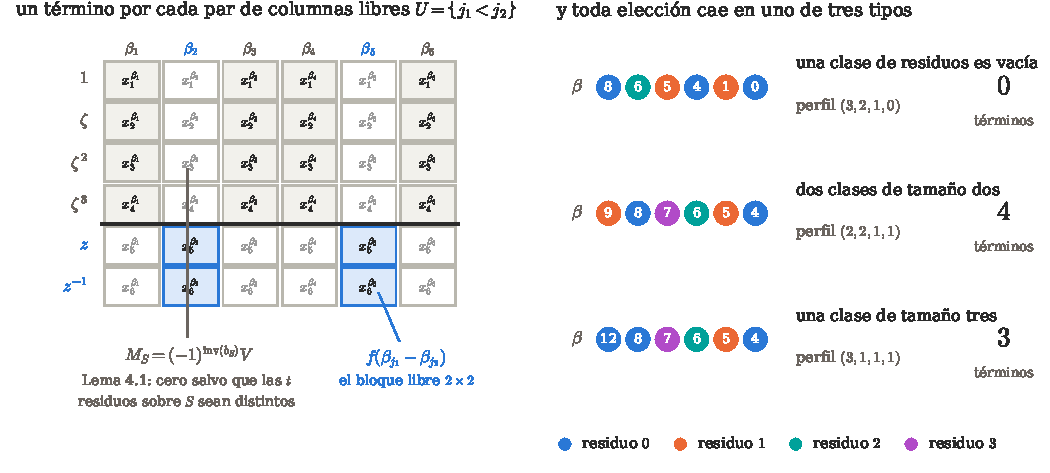
\includegraphics[width=\textwidth]{fig_laplace_es.pdf}
\caption{La arquitectura de la demostración, dibujada con $t=4$, $N=6$. \emph{Izquierda:} el
determinante $\det(x_i^{\beta_j})$ desarrollado por las $t$ filas congeladas. Cada elección de las
dos columnas $U=\{j_1<j_2\}$ que se dejan a las filas libres $z,z^{-1}$ deja un menor $t\times t$
$M_S$ sobre las columnas complementarias, que por el Lema \ref{lem:L1} vale $\pm V$ o cero, por el
bloque $2\times2$ $f(\beta_{j_1}-\beta_{j_2})$. \emph{Derecha:} por el recuento del exceso dos
\eqref{eq:excess} sólo hay tres perfiles de residuos, uno por fila, cada uno sobre un beta-conjunto
que lo realiza; el número de la derecha es cuántas elecciones de $U$ sobreviven, contado y no
afirmado --- $0$, $4$ y $3$, que es la tricotomía sobre la que se organiza la sección. El color es
la clase de residuos. Calculada por \texttt{anc/fig\_proof.py}.}
\label{fig:laplace}
\end{figure}

El desarrollo en sí es el movimiento habitual de esta literatura y no reclamamos nada por él: Albion
\cite{Alb25} aplica el desarrollo de Laplace a un determinante de esta forma \emph{según la
estructura de bloques dada}, manteniendo fijo un primer conjunto de filas, siguiendo a Krattenthaler
y a Ciucu--Krattenthaler. Lo particular aquí no es el desarrollo, sino con qué se topa.

Lo que el argumento hace en realidad es clasificar, no calcular. Desarrollar por las $t$ filas
congeladas deja un término por cada manera de elegir qué dos columnas \emph{no} lo están, y el
recuento del exceso dos dice que toda elección cae en exactamente uno de tres tipos combinatorios:
no sobrevive ninguna (una clase de residuos es vacía), sobreviven cuatro (dos clases de tamaño dos) o
sobreviven tres (una clase de tamaño tres). Todo lo que sigue es contabilidad dentro de un tipo, y el
Lema \ref{lem:L5} muestra que los dos últimos son un mismo enunciado visto dos veces. La Figura \ref{fig:laplace} es esa frase dibujada.

\begin{lemma}\label{lem:L1}
Sea $S$ un conjunto de $t$ columnas y $M_S=\det(\zeta^{k\beta_j})_{0\le k<t,\,j\in S}$. Entonces
$M_S=0$ salvo que los residuos $\{\beta_j\bmod t:j\in S\}$ sean dos a dos distintos, en cuyo caso
$M_S=(-1)^{\inv(b_S)}V$.
\end{lemma}

\begin{proof}
Como $\zeta^{k\beta_j}=(\zeta^{\beta_j})^k$, la matriz es de Vandermonde en los valores
$y_j=\zeta^{\beta_j}$, cuyo determinante es $\prod_{j<j'}(y_{j'}-y_j)$. El valor $y_j$ depende de
$\beta_j$ solo módulo $t$, luego dos columnas de $S$ que compartan residuo anulan el determinante. Si
los residuos son dos a dos distintos, $|S|=t$ obliga a $\{y_j\}_{j\in S}=\zt$ como conjunto, y el
determinante de Vandermonde es alternante en sus argumentos, luego vale $V$ por el signo de la
permutación que ordena $b_S$ crecientemente, que es $(-1)^{\inv(b_S)}$.
\end{proof}

\begin{lemma}\label{lem:L2}
$\det\bigl(x_i^{N-j}\bigr)_{i,j=1}^{N}=(-1)^{\binom t2}\,V\,(z^t-1)(z^{-t}-1)(z-z^{-1})$ para el
alfabeto $x=(1,\zeta,\dots,\zeta^{t-1},z,z^{-1})$ en ese orden.
\end{lemma}

\begin{proof}
El determinante es $\prod_{i<i'}(x_i-x_{i'})$. Los pares dentro de $\zt$ aportan
$\prod_{k<k'}(\zeta^k-\zeta^{k'})=(-1)^{\binom t2}V$; los pares $(\zeta^k,z)$ aportan
$\prod_k(\zeta^k-z)=(-1)^t(z^t-1)$ y los pares $(\zeta^k,z^{-1})$ aportan $(-1)^t(z^{-t}-1)$; el
último par aporta $z-z^{-1}$. Los dos factores $(-1)^t$ se cancelan.
\end{proof}

\noindent Lo calculamos porque son tres líneas, no porque sea desconocido: un determinante sobre un
alfabeto cerrado bajo $x\mapsto x^{-1}$, evaluado en forma de producto cerrado, es exactamente el
asunto del complemento de Krattenthaler al cálculo de determinantes \cite[\S5.11]{KratADCC}, cuyo
Lema 20 lleva entre sus casos particulares las fórmulas del denominador de Weyl para $B_n$, $C_n$ y
$D_n$. Lo que esa literatura no evalúa ---y lo que el lema siguiente necesita--- es ese mismo
determinante con una órbita de raíces de la unidad dentro del alfabeto.

\begin{lemma}\label{lem:L3}
Sea $\mathcal U$ el conjunto de pares $U=\{j_1<j_2\}$ de columnas cuyo complementario $S_U$ lleva las
$t$ clases de residuos. Entonces
\[
\Phi_t(\lambda;z)=\frac{(-1)^{\,t+\binom{N+1}{2}}}{(z^t-1)(z^{-t}-1)(z-z^{-1})}
\sum_{U\in\mathcal U}(-1)^{\,j_1+j_2+\inv(b_{S_U})}\,f(\beta_{j_1}-\beta_{j_2}).
\]
\end{lemma}

\begin{proof}
Desarrollando el numerador por Laplace a lo largo de las primeras $t$ filas,
\[
\det\bigl(x_i^{\beta_j}\bigr)=\sum_{|S|=t}(-1)^{\binom{t+1}{2}+\sum_{j\in S}j}\,M_S\,C_{S^c},
\]
donde para $S^c=\{j_1<j_2\}$ el menor complementario $2\times2$ es
$z^{\beta_{j_1}-\beta_{j_2}}-z^{-(\beta_{j_1}-\beta_{j_2})}=f(\beta_{j_1}-\beta_{j_2})$. Por el Lema
\ref{lem:L1} solo contribuyen los $S$ con residuos dos a dos distintos. Escribiendo
$\sum_{j\in S}j=\binom{N+1}{2}-j_1-j_2$ y dividiendo por el Lema \ref{lem:L2}, los factores $V$ se
cancelan y $(-1)^{\binom{t+1}{2}-\binom{t}{2}}=(-1)^t$.
\end{proof}

Si algún $n_i=0$, ningún $S$ de tamaño $t$ lleva todos los residuos, $\mathcal U=\varnothing$ y
$\Phi_t=0$: es el Teorema \ref{thm:main}(i). En caso contrario todos los $n_i\ge1$ y por
\eqref{eq:excess} o bien dos clases tienen tamaño dos, y entonces $S_U$ debe descartar un elemento de
cada una y $|\mathcal U|=4$, o bien una clase tiene tamaño tres, y entonces $S_U$ descarta dos de los
tres y $|\mathcal U|=3$.

\begin{lemma}[el movimiento de columna]\label{lem:L4}
Sean $A$ y $B$ clases distintas de tamaño dos, en las columnas $j_{A_1}<j_{A_2}$ y
$j_{B_1}<j_{B_2}$. Para $i,j\in\{1,2\}$ sea $U_{ij}$ el par formado por la columna de $a_i$ y la de
$b_j$, y sea $\kappa_{ij}=(-1)^{\,j_{A_i}+j_{B_j}+\inv(b_{S_{U_{ij}}})}\sgn(a_i-b_j)$, de modo que
el término $U_{ij}$ del Lema \ref{lem:L3} vale $\kappa_{ij}f(a_i-b_j)$. Entonces
$\kappa_{ij}=\kappa_{11}(-1)^{i-1}(-1)^{j-1}$.
\end{lemma}

\begin{proof}
Fijemos $j$ y comparemos $i=1$ con $i=2$. Los conjuntos $S_{U_{1j}}$ y $S_{U_{2j}}$ difieren solo en
que el primero contiene la columna $j_{A_2}$ y el segundo la columna $j_{A_1}$, y la letra que llevan
es el residuo $r_A$ en ambos casos. Pasar de una palabra a la otra mueve esa letra a través de
exactamente las columnas conservadas estrictamente entre $j_{A_1}$ y $j_{A_2}$, y ninguna de esas
letras es igual a $r_A$ porque la clase $A$ tiene solo dos elementos; cada cruce cambia la paridad de
$\inv$. Por tanto
\[
(-1)^{\inv(b_{S_{U_{1j}}})-\inv(b_{S_{U_{2j}}})}
=(-1)^{(j_{A_2}-j_{A_1}-1)-[\,a_2<b_j<a_1\,]},
\]
usando que $\beta$ es estrictamente decreciente en el índice de columna, de modo que $j_{B_j}$ está
estrictamente entre $j_{A_1}$ y $j_{A_2}$ exactamente cuando $a_2<b_j<a_1$. Multiplicando por el
factor de Laplace $(-1)^{j_{A_1}+j_{A_2}}$,
\[
\frac{\kappa_{1j}}{\kappa_{2j}}
=(-1)^{2j_{A_2}-1}(-1)^{[\,a_2<b_j<a_1\,]}\sgn(a_1-b_j)\sgn(a_2-b_j)=-1,
\]
porque $\sgn(a_1-b_j)\sgn(a_2-b_j)=-1$ exactamente cuando $b_j$ está entre $a_2$ y $a_1$.
Intercambiando los papeles de $A$ y $B$ se obtiene $\kappa_{i1}/\kappa_{i2}=-1$.
\end{proof}

\begin{lemma}\label{lem:L5}
Para todos $c,p,q$ y todos $u,v$,
\begin{align*}
\text{\rm(a)}&\quad \sum_{\epsilon,\eta\in\{\pm1\}}\epsilon\eta\,f(c+\epsilon p+\eta q)=f(c)f(p)f(q),\\
\text{\rm(b)}&\quad f(2u)-f(2u+2v)+f(2v)=-f(u)f(v)f(u+v).
\end{align*}
\end{lemma}

\begin{proof}
Para (a), $\sum_{\epsilon,\eta}\epsilon\eta\,z^{c+\epsilon p+\eta q}
=z^{c}\bigl(\sum_\epsilon\epsilon z^{\epsilon p}\bigr)\bigl(\sum_\eta\eta z^{\eta q}\bigr)
=z^{c}f(p)f(q)$, y el mismo cálculo para los exponentes negativos da $z^{-c}(-f(p))(-f(q))$;
réstese. Para (b), pónganse $s=z^u$, $w=z^v$ y desarróllese
$(s-s^{-1})(w-w^{-1})(sw-s^{-1}w^{-1})$: los ocho términos se recombinan como
$(s^2w^2-s^{-2}w^{-2})-(s^2-s^{-2})-(w^2-w^{-2})=f(2u+2v)-f(2u)-f(2v)$.
\end{proof}

\begin{proof}[Demostración del Teorema \ref{thm:main}]
En el perfil de dos clases, los Lemas \ref{lem:L3} y \ref{lem:L4} dan
\[
\sum_{U\in\mathcal U}(\cdots)=\kappa_{11}\sum_{i,j}(-1)^{i-1}(-1)^{j-1}f(a_i-b_j).
\]
Escribiendo $a_i=\alpha+\epsilon_ip$ y $b_j=\gamma+\eta_jq$ con $p=d_1/2$, $q=d_2/2$ y
$\epsilon=\eta=(+1,-1)$, se tiene $a_i-b_j=c+\epsilon_ip-\eta_jq$ con $c=\alpha-\gamma$. Sustituyendo
$\eta$ por $-\eta$, la suma se convierte en
$-\sum_{\epsilon,\eta}\epsilon\eta f(c+\epsilon p+\eta q)$, que vale $-f(c)f(p)f(q)$ por el Lema
\ref{lem:L5}(a). Como $(z^t-1)(z^{-t}-1)=2-z^t-z^{-t}=-f(t/2)^2$ y $z-z^{-1}=f(1)$, los dos signos
menos se cancelan, y sustituyendo $f(u)=2\sinh(u\theta)$ los factores numéricos se cancelan. Aquí
$2c=\tilde d_3$. Si $\tilde d_3=0$, entonces $f(c)=0$ y la suma entera se anula, que es la primera
afirmación de {\rm(ii)}; en caso contrario
$\sinh(c\theta)=\sgn(\tilde d_3)\sinh(d_3\theta/2)$, lo que da \eqref{eq:main} con
$\varepsilon_\lambda=(-1)^{\,t+\binom{N+1}{2}}\kappa_{11}\sgn(\tilde d_3)$, que es
\eqref{eq:sign} por la definición de $\kappa_{11}$ en el Lema \ref{lem:L4}.

Para el perfil de tamaño tres $\{p>q>r\}$ en las columnas $j_1<j_2<j_3$ se aplica el mismo argumento
de movimiento de columna, de nuevo porque ninguna letra estrictamente entre dos de esas columnas
lleva el residuo de la clase, y da signos alternantes $(\varsigma,-\varsigma,\varsigma)$ para los
tres términos $f(p-q)$, $f(p-r)$, $f(q-r)$. Por el Lema \ref{lem:L5}(b) con $u=(p-q)/2$,
$v=(q-r)/2$ la suma es $-\varsigma f(u)f(v)f(u+v)$, que es la fórmula de dos clases para $A=\{p,q\}$,
$B=\{q,r\}$ con $\varsigma=\kappa_{11}$. Equivalentemente, la cuarta selección ausente del perfil de
dos clases descartaría $q$ dos veces y su término lleva $f(0)=0$, de modo que los dos perfiles son un
solo enunciado.
\end{proof}

Todos los enunciados de este artículo se comprobaron además numéricamente; los recuentos se recogen
una sola vez, en la \S\ref{sec:verif}, en lugar de repetirse según van surgiendo.

%======================================================================
\section{Independencia en el lugar recíproco}\label{sec:independence}

El Teorema 5.3 de \cite{AK25} está enunciado para variables libres, y $(z,\zb)$ no es un par libre.
Nada de esta sección lo contradice: el lugar recíproco queda fuera de sus hipótesis, no en contra de
ellas, y lo que hacemos aquí es determinar en qué se convierte allí su criterio. Leída al pie de la
letra, \eqref{eq:AK53} diría que para $\ell(\lambda)\le2$ se tiene
$s_\lambda(z,\zb,\zt)=s_\lambda(z,\zb)$ exactamente sobre los $t$-núcleos. El Teorema
\ref{thm:main} evalúa el miembro izquierdo para toda $\lambda$, y al comparar ambos se ve que el
lugar recíproco lleva más soluciones: exactamente una familia. Medir cuánto sobrevive un criterio a
una degeneración es una manera de decir lo afilado que era, y la respuesta aquí es que lo es salvo
una sola familia.

Aislamos primero cuándo $\Phi_t$ degenera en un solo carácter.

\begin{lemma}\label{lem:single}
$\Phi_t(\lambda;z)=\pm\chi_k(z)$ para algún $k\ge0$ si y solo si el multiconjunto $\{d_1,d_2,d_3\}$
contiene $t$ al menos dos veces, y en tal caso la entrada restante vale $2(k+1)$.
\end{lemma}

\begin{proof}
Pongamos $u=z^{1/2}$, de modo que $2\sinh(d_i\theta/2)=u^{d_i}-u^{-d_i}$,
$2\sinh(t\theta/2)=u^{t}-u^{-t}$ y $2\sinh\theta=u^{2}-u^{-2}$; todos los exponentes son enteros. Por
\eqref{eq:main}, la igualdad afirmada es
\[
\prod_{i=1}^{3}\bigl(u^{d_i}-u^{-d_i}\bigr)
=\pm\bigl(u^{t}-u^{-t}\bigr)^{2}\bigl(u^{2k+2}-u^{-2k-2}\bigr).
\]
Usando $u^{n}-u^{-n}=u^{-n}(u^{2n}-1)$ en cada factor y comparando los prefactores monomiales se
obtiene $d_1+d_2+d_3=2t+2(k+1)$ junto con
\[
\prod_{i=1}^{3}\bigl(u^{2d_i}-1\bigr)=\pm\bigl(u^{2t}-1\bigr)^{2}\bigl(u^{4(k+1)}-1\bigr),
\]
y evaluando en $u=0$ el signo queda fijado en $+$. Ahora $u^{2n}-1=\prod_{m\mid 2n}Q_m(u)$ con
$Q_m$ los polinomios ciclotómicos como en la Proposición \ref{prop:minimal}, que son irreducibles y
distintos dos a dos, de modo que por
factorización única en $\ZZ[u]$ ambos miembros tienen el mismo multiconjunto de factores
ciclotómicos. A la izquierda ese multiconjunto es $\biguplus_i\{m:m\mid 2d_i\}$ y a la derecha
$2\times\{m:m\mid 2t\}\uplus\{m:m\mid 4(k+1)\}$. Su mayor elemento es $\max_i 2d_i$ a la izquierda y
$\max(2t,4(k+1))$ a la derecha; borrando de ambos lados el conjunto de divisores de ese máximo y
repitiendo dos veces más se llega a
\[
\{2d_1,2d_2,2d_3\}=\{2t,\,2t,\,4(k+1)\}
\]
como multiconjuntos, que es lo afirmado. El recíproco es el mismo cálculo leído al revés.
\end{proof}

\begin{theorem}\label{thm:extra}
Sea $\ell(\lambda)\le2$. Entonces
\[
\Phi_t(\lambda;z)=s_\lambda(z,\zb)
\]
---una igualdad, y no una igualdad salvo signo--- si y solo si o bien
$\lambda=\core_t(\lambda)$, o bien
\begin{equation}\label{eq:extra}
t\ \text{es par}\quad\text{y}\quad \lambda=\Bigl(\lambda_2+\tfrac{3t}{2}-1,\ \lambda_2\Bigr)
\quad\text{con}\quad \tfrac t2\le\lambda_2\le t-1 .
\end{equation}
En el segundo caso $\{d_1,d_2,d_3\}=\{3t,t,t\}$ y $\varepsilon_\lambda=+1$, mientras que
$\core_t(\lambda)=\bigl(\tfrac t2-1+j,j\bigr)$ y $\quot_t(\lambda)$ tiene como única componente no
vacía $(2)$, en la posición $j=\lambda_2-\tfrac t2$.
\end{theorem}

La Figura \ref{fig:locus} es el enunciado computado en vez de afirmado: ambas familias están
dibujadas sobre un rango de $t$, y el $t$ impar donde \eqref{eq:extra} no puede darse es el control.

\begin{figure}[!ht]
\centering
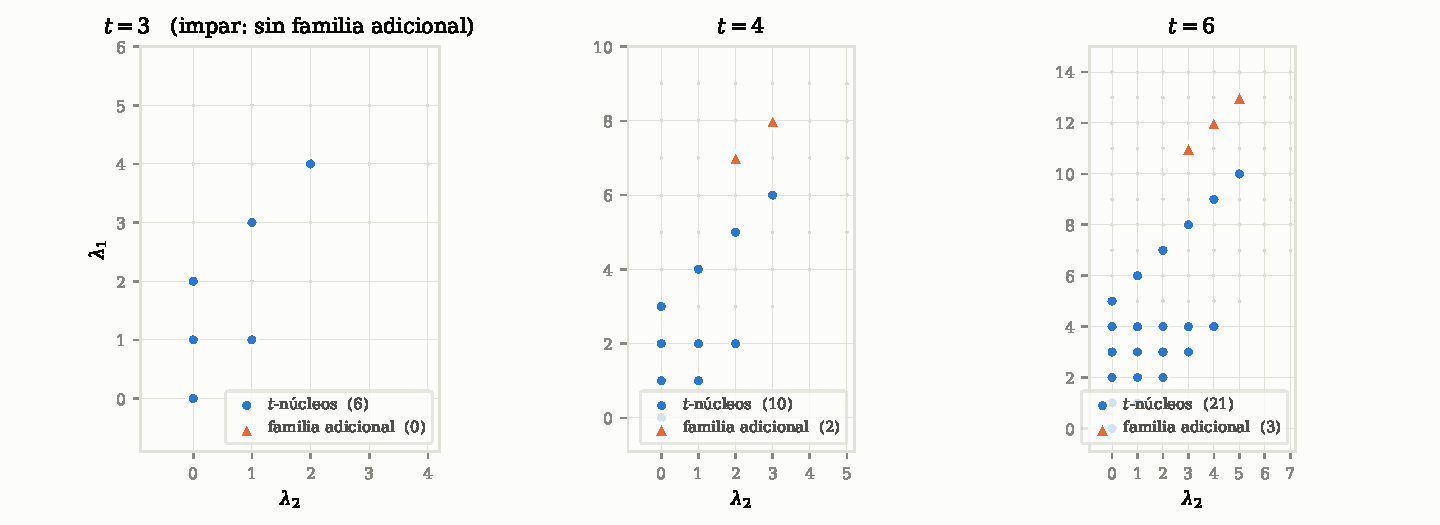
\includegraphics[width=\textwidth]{fig_locus_es.pdf}
\caption{El Teorema \ref{thm:extra}, calculado y no afirmado. Para toda $\lambda$ de dos filas en
rango se evaluaron ambos miembros de $\Phi_t(\lambda;z)=\pm s_\lambda(z,\zb)$; se representan las
particiones donde coinciden, coloreadas por familia. Los círculos son los $t$-núcleos, las soluciones
ya descritas por \eqref{eq:AK53}; los triángulos son la familia adicional \eqref{eq:extra}, que crea
la especialización recíproca. El caso impar $t=3$ es el control: por el Teorema \ref{thm:extra} allí
no puede existir solución adicional, y no se halla ninguna.}
\label{fig:locus}
\end{figure}

\begin{proof}
Como $\ell(\lambda)\le 2$ y $N=t+2$, el conjunto beta es
$\beta(\lambda)=\bigl(A'+t,\;B'+t,\;t-1,t-2,\dots,1,0\bigr)$ donde
\[
A':=\lambda_1+1,\qquad B':=\lambda_2,\qquad A'>B'\ge0 .
\]
El bloque $\{0,1,\dots,t-1\}$ toca cada clase de residuos exactamente una vez, luego ninguna clase es
vacía y las dos partes grandes deciden el perfil. Escribamos $A'=t\alpha+\rho_A$ y
$B'=t\gamma+\rho_B$ con $0\le\rho_A,\rho_B\le t-1$. Como $s_\lambda(z,\zb)=\chi_{\lambda_1-\lambda_2}(z)$,
el Lema \ref{lem:single} dice que la afirmación se cumple exactamente cuando $\{d_1,d_2,d_3\}$
contiene $t$ dos veces y la tercera entrada es $2(\lambda_1-\lambda_2+1)=2(A'-B')$.

\emph{Caso $\rho_A=\rho_B=:\rho$.} Una clase tiene tamaño tres, a saber $\{A'+t,B'+t,\rho\}$, y por el
Teorema \ref{thm:main} los tres argumentos son $d_1=A'-B'$, $d_2=B'+t-\rho=t(\gamma+1)$,
$d_3=A'+t-\rho=t(\alpha+1)$. Aquí $t\mid A'-B'$, digamos $A'-B'=ts$ con $s\ge1$. El par $d_2=d_3=t$
fuerza $\alpha=\gamma=0$, luego $A'=B'$, excluido. El par $d_1=d_3=t$ fuerza $s=1$ y $\alpha=0$,
luego $A'<t$ y $A'=B'+t\ge t$, excluido. El par $d_1=d_2=t$ fuerza $s=1$ y $\gamma=0$, es decir
$A'=B'+t$ con $B'<t$; entonces $\alpha=1$ y la tercera entrada es $d_3=2t=2(A'-B')$, como se
requiere. Este caso aporta pues exactamente las $\lambda$ con $A'=B'+t$, $B'<t$.

\emph{Caso $\rho_A\ne\rho_B$.} Dos clases tienen tamaño dos, a saber $\{A'+t,\rho_A\}$ y
$\{B'+t,\rho_B\}$, y los tres argumentos son
\[
d_A=t(\alpha+1),\qquad d_B=t(\gamma+1),\qquad
d_3=\bigl|\,t(\alpha-\gamma)+2(\rho_A-\rho_B)\,\bigr| .
\]
Si $d_A=d_B=t$ entonces $\alpha=\gamma=0$, luego $A',B'<t$ y $d_3=2|\rho_A-\rho_B|=2(A'-B')$
automáticamente: toda tal $\lambda$ es solución. En otro caso exactamente uno de $d_A,d_B$ vale $t$ y
$d_3=t$. Si $\alpha=0$ y $\gamma\ge1$, entonces $|-t\gamma+2(\rho_A-\rho_B)|=t$ con
$|\rho_A-\rho_B|\le t-1$ fuerza $\gamma=2$ y $\rho_A-\rho_B=t/2$; pero entonces
$\lambda_1=A'-1=\rho_A-1<t$ mientras que $\lambda_2=B'\ge2t$, en contra de $\lambda_1\ge\lambda_2$.
Si $\gamma=0$ y $\alpha\ge1$, entonces $|t\alpha+2(\rho_A-\rho_B)|=t$ fuerza, para $\alpha=1$,
$\rho_A=\rho_B$ (excluido), y para $\alpha=2$,
\[
\rho_B-\rho_A=\tfrac t2,
\]
lo que exige $t$ par; $\alpha\ge3$ da $|2(\rho_A-\rho_B)|\ge2t$, imposible. Luego $A'=2t+\rho_A$,
$B'=\rho_B=\rho_A+\tfrac t2$, de donde
\[
\lambda_1=2t+\rho_A-1,\qquad \lambda_2=\rho_A+\tfrac t2,\qquad
\lambda_1-\lambda_2=\tfrac{3t}{2}-1,
\]
y $\rho_B\le t-1$ da $0\le\rho_A\le\tfrac t2-1$, es decir $\tfrac t2\le\lambda_2\le t-1$. La entrada
restante es $d_A=t(\alpha+1)=3t=2(\lambda_1-\lambda_2+1)$, como se requiere. Esto es
\eqref{eq:extra}.

Queda identificar las soluciones del primer caso de cada análisis con los $t$-núcleos. Para
$\ell(\lambda)\le2$ el conjunto beta en dos posiciones es $(A',B')$, y $\lambda$ es un $t$-núcleo si
y solo si ningún número beta puede rebajarse en $t$ hasta una posición no negativa desocupada, es
decir si y solo si $B'<t$ y o bien $A'<t$ o bien $A'=B'+t$. Son exactamente las dos familias
halladas. Por último, en el caso \eqref{eq:extra} la clase $\rho_A$ lleva $\{2t+\rho_A+t,\rho_A\}$,
luego su componente del cociente es $(2)$, toda otra componente es vacía, y el núcleo es el
enunciado.

\emph{El signo.} Las dos familias lo consiguen por razones distintas. Sobre los $t$-núcleos la
igualdad es \eqref{eq:AK53} misma, que es una igualdad y no una igualdad salvo signo, así que no hay
nada que probar. Sobre \eqref{eq:extra}, escríbase $t=2m$ y $\lambda_2=m+j$ con $0\le j\le m-1$, de
modo que $\rho_A=j$ y $\rho_B=m+j$ y
\[
\beta(\lambda)=\bigl(6m+j,\;3m+j,\;2m-1,2m-2,\dots,1,0\bigr).
\]
Reduciendo módulo $t=2m$, la palabra de residuos leída en orden creciente de columna es
\[
w=\bigl(j,\;m+j,\;2m-1,2m-2,\dots,1,0\bigr),
\]
puesto que $6m+j\equiv j$ y $3m+j\equiv m+j$, esto último porque $j\le m-1$. Sus inversiones son de
tres clases: la cola decreciente aporta $\binom{2m}{2}$; la primera letra está por encima de
exactamente las $j$ letras de la cola $0,\dots,j-1$; la segunda, por encima de exactamente las $m+j$
letras $0,\dots,m+j-1$; y las dos primeras letras están en orden creciente, así que no aportan
ninguna. Por tanto
\begin{equation}\label{eq:extrainv}
\inv(w)=\binom{2m}{2}+j+(m+j)=2m^{2}+2j\;\equiv\;0\pmod2 ,
\end{equation}
luego $\sgn(\sigma)=(-1)^{\inv(w)}=+1$ por la primera línea de la prueba de la Proposición
\ref{rem:sign}. Las dos clases distinguidas son $r_A=j<r_B=m+j$, que llevan $A=\{6m+j,\,j\}$ y
$B=\{3m+j,\,m+j\}$, de modo que $\tilde d_3=(6m+2j)-(4m+2j)=2m>0$ y $\sgn(\tilde d_3)=+1$. Los dos
factores restantes de \eqref{eq:shortsign} son $(-1)^{\lfloor t/2\rfloor}=(-1)^{m}$ y
$(-1)^{r_A+r_B}=(-1)^{m+2j}=(-1)^{m}$, cuyo producto es $+1$. Así pues $\varepsilon_\lambda=+1$, y
como $d_1=6m=3t$, $d_2=2m=t$ y $d_3=2m=t$, \eqref{eq:main} dice
\[
\Phi_t(\lambda;z)=\frac{\sinh(3t\theta/2)\sinh^{2}(t\theta/2)}{\sinh^{2}(t\theta/2)\sinh\theta}
=\chi_{\frac{3t}{2}-1}(z)=\chi_{\lambda_1-\lambda_2}(z)=s_\lambda(z,\zb),
\]
sin ningún signo que arrastrar.
\end{proof}

\noindent Lo que compra \eqref{eq:extrainv} no es decoración. Enunciado salvo signo, el Teorema
\ref{thm:extra} dice que la especialización crea una familia de formas sobre las que el twist es
invisible \emph{salvo un signo}, que es un enunciado más débil que el que \eqref{eq:AK53} hace sobre
los núcleos; con el signo resuelto, las dos familias son soluciones de la misma ecuación, y ``el
lugar recíproco adquiere exactamente una familia más'' es literalmente cierto.

\begin{remark}\label{rem:why}
El Lema \ref{lem:single} controla el valor sólo salvo signo, y por eso el signo del Teorema
\ref{thm:extra} necesita el párrafo aparte de arriba en lugar de salir de la clasificación.

La familia adicional pertenece a la especialización y no al alfabeto. El paso es el
\cite[Lema 5.2]{AK25}, sobre el que se apoya el \cite[Teorema 5.3]{AK25}: reduce la independencia a
la anulación de $s_{\lambda/\mu}$ en el alfabeto torcido para todo $\mu\subsetneq\lambda$, y la
reducción usa la independencia lineal de los caracteres universales $f_\mu$ en las variables libres. En el lugar recíproco
$s_\mu(z,\zb)=\chi_{\mu_1-\mu_2}(z)$ depende solo de $\mu_1-\mu_2$, luego $s_{(1)}$, $s_{(2,1)}$ y
$s_{(3,2)}$ coinciden allí y esa independencia deja de estar disponible; el Teorema \ref{thm:extra}
mide la diferencia. Un control confirma la lectura: para $\lambda=(3,1)$ y $t=2$ se tiene
$s_\lambda(\zt,z,\zb)=s_\lambda(z,\zb)$, mientras que $s_\lambda(\zt,x,y)\ne s_\lambda(x,y)$ para
$x,y$ libres.
\end{remark}

Así pues, el criterio no sobrevive intacto a la especialización, y lo que adquiere es pequeño y
nombrable: una familia, para formas de dos filas, indexada por un elemento de orden dos del retículo
de residuos y clasificada por su núcleo y su cociente. Las soluciones adicionales pertenecen al lugar
recíproco y no al alfabeto ---existen porque una especialización ha retirado una independencia lineal
que el argumento original usaba, y ese paso que falta es exactamente lo que mide el Teorema
\ref{thm:extra}.

%======================================================================
\section{Una enumeración en la que sobrevive un parámetro}\label{sec:enum}

Desarrollando $s_\lambda$ sobre tablas semiestándar, el Teorema \ref{thm:main} se convierte en una
fórmula de producto para un recuento pesado. Sea $m_k(T)$ el número de entradas iguales a $k$ en $T$.

\begin{corollary}\label{cor:enum}
Desarrollando $s_\lambda$ sobre tablas semiestándar y aplicando el Teorema \ref{thm:main}: para todo
$t\ge2$ y toda $\lambda\in\PP_{t+2}$,
\[
\sum_{T\in\mathrm{SSYT}(\lambda,\,t+2)}
\zeta^{\,\sum_{k=1}^{t}(k-1)m_k(T)}\;z^{\,m_{t+1}(T)-m_{t+2}(T)}
\;=\;\varepsilon_\lambda\,
\frac{\sinh(d_1\theta/2)\sinh(d_2\theta/2)\sinh(d_3\theta/2)}{\sinh^2(t\theta/2)\sinh\theta}.
\]
\end{corollary}

Para $t=2$ el peso es $(-1)^{m_2(T)}$, y si $\lambda=(c^{\,a})$ es rectangular entonces
$\mathrm{SSYT}(\lambda,4)$ está en biyección con las particiones planas en una caja
$a\times(4-a)\times c$, equivalentemente con las teselaciones de rombos de un hexágono. El Corolario
\ref{cor:enum} es entonces una $(-1)$-enumeración de esos objetos \emph{refinada por un parámetro
libre} $z$, que registra la diferencia entre los números de entradas $3$ y $4$. Poniendo $z=1$ se
recupera el recuento con signo puro, que por \eqref{eq:main} vale $\pm d_1d_2d_3/(2t^2)$: para la
$a=2$, $c=2$ vale $4$; para $a=2$, $c=4$ vale $9$; para $a=3$, $c=3$ vale $-6$.

\begin{example}\label{ex:boxes}
Tomando $\lambda=(c^{\,a})$ con $1\le a\le4$ y $t=2$, la forma tiene a lo sumo cuatro filas, las
tablas son las particiones planas en una caja $a\times(4-a)\times c$, y la forma cerrada da los
recuentos con signo de la Figura \ref{fig:signed}. Leyéndola:
\[
\begin{array}{ll}
1\times3\times c: & \bigl\lfloor (c+2)^2/4\bigr\rfloor,\\[2pt]
2\times2\times c: & (c/2+1)^2 \text{ si } c \text{ es par},\qquad 0 \text{ si } c \text{ es impar},\\[2pt]
3\times1\times c: & (-1)^c\bigl\lfloor (c+2)^2/4\bigr\rfloor,\\[2pt]
4\times0\times c: & (-1)^c .
\end{array}
\]
La tercera fila es la traspuesta de la primera, y por eso los módulos coinciden; la cuarta es la caja
degenerada, donde $s_{(c^4)}(x)=(x_1x_2x_3x_4)^c$ y el alfabeto tiene determinante $-1$. No
reivindicamos estos recuentos concretos como nuevos ---las cajas son pequeñas y el signo aquí es la
especialización $x_2=-1$, no el signo de complementación de las $(-1)$-enumeraciones de Kuperberg---
y los registramos solo para mostrar lo que produce el teorema. Lo que sí parece nuevo es que cada uno
de ellos es el valor en $z\mapsto1$ de un refinamiento de un parámetro con la misma fórmula de
producto.
\end{example}

Los cuadrados perfectos del Ejemplo \ref{ex:boxes} no son un accidente de casos pequeños: son lo que
la lectura por intervalos de la \S\ref{sec:intervals} dice que un rectángulo debe producir.

\begin{proposition}\label{prop:rect}
Sean $t=2$ y $\lambda=(c^{\,a})$ con $1\le a\le4$. Entonces uno de $d_1,d_2,d_3$ vale $2$, y:
\begin{enumerate}
\item[\rm(i)] si $a=4$, los tres valen $2$ sea cual sea $c$ y el recuento es $(-1)^c$: es el
rectángulo completo, donde $s_{(c^4)}(x)=(x_1x_2x_3x_4)^{c}$ se reduce a un monomio y del alfabeto no
queda más que su determinante;
\item[\rm(ii)] si $a\le3$ y $c$ es par, los otros dos valen ambos $c+2$, de modo que los dos
intervalos tienen \emph{la misma longitud} y el recuento con signo es el cuadrado perfecto
$\bigl(\tfrac{c+2}{2}\bigr)^2$;
\item[\rm(iii)] si $c$ es impar y $a=2$, los dos intervalos son \emph{concéntricos} y el recuento es
$0$;
\item[\rm(iv)] si $c$ es impar y $a\in\{1,3\}$, los otros dos valen $c+1$ y $c+3$, y el recuento es
$\pm\tfrac{(c+1)(c+3)}{4}=\pm\bigl\lfloor\tfrac{(c+2)^2}{4}\bigr\rfloor$.
\end{enumerate}
El caso {\rm(i)} no es una degeneración del triple de intervalos sino un colapso de la forma misma, y
es el único en el que la paridad de $c$ no interviene.
\end{proposition}

\begin{proof}
Para $\lambda=(c^{\,a})$ el conjunto beta consta de dos bloques de enteros consecutivos, a saber
$c+3,c+2,\dots,c+4-a$ y $3-a,2-a,\dots,0$; los residuos alternan a lo largo de cada bloque, y eso es
lo que fuerza las coincidencias. Explícitamente, para $a=1,2,3,4$ el conjunto beta es $(c+3,2,1,0)$,
$(c+3,c+2,1,0)$, $(c+3,c+2,c+1,0)$ y $(c+3,c+2,c+1,c)$. Separando cada uno por paridad se obtiene,
para $c$ par,
\[
\{c{+}3,1\},\{2,0\};\qquad \{c{+}3,1\},\{c{+}2,0\};\qquad \{c{+}3,c{+}1\},\{c{+}2,0\};\qquad
\{c{+}3,c{+}1\},\{c{+}2,c\},
\]
de donde $(d_1,d_2,d_3)$ vale $(c{+}2,2,c{+}2)$, $(c{+}2,c{+}2,2)$, $(2,c{+}2,c{+}2)$ y $(2,2,2)$
respectivamente; en cada caso el producto dividido por $2t^2=8$ es $\bigl(\tfrac{c+2}{2}\bigr)^2$,
resp. $1$. Para $c$ impar y $a=2$ la separación es $\{c{+}3,0\},\{c{+}2,1\}$, luego
$d_3=|c{+}3+0-c{-}2-1|=0$: los intervalos son concéntricos y se aplica el Corolario \ref{cor:zero}.
Para $c$ impar y $a=1,3$ la paridad pone tres números beta en una misma clase, $\{c{+}3,2,0\}$ y
$\{c{+}3,c{+}1,0\}$ respectivamente, y el perfil de tamaño tres da $(c{+}1,2,c{+}3)$ y
$(2,c{+}1,c{+}3)$, con producto dividido por $8$ igual a $\tfrac{(c+1)(c+3)}{4}$. Para $c$ impar y
$a=4$ los cuatro números beta vuelven a ser consecutivos, así que la separación es
$\{c{+}3,c{+}1\},\{c{+}2,c\}$ y el triple es $(2,2,2)$ igual que para $c$ par: a altura completa el
resultado no ve la paridad de $c$, y por eso $a=4$ va aparte.
\end{proof}

Así pues el cuadrado es el cuadrado de la mitad de la longitud común de los intervalos, los ceros son
las configuraciones concéntricas, los cuartos de cuadrado son el caso en que las dos longitudes
difieren en $2$, y a altura completa los tres intervalos coinciden, la forma se vuelve un monomio y no
sobrevive más que un signo. Qué par de los tres coincide rota con $a$, y por eso el mismo valor
reaparece en columnas distintas de la Figura \ref{fig:signed}.

\begin{figure}[t]
\centering
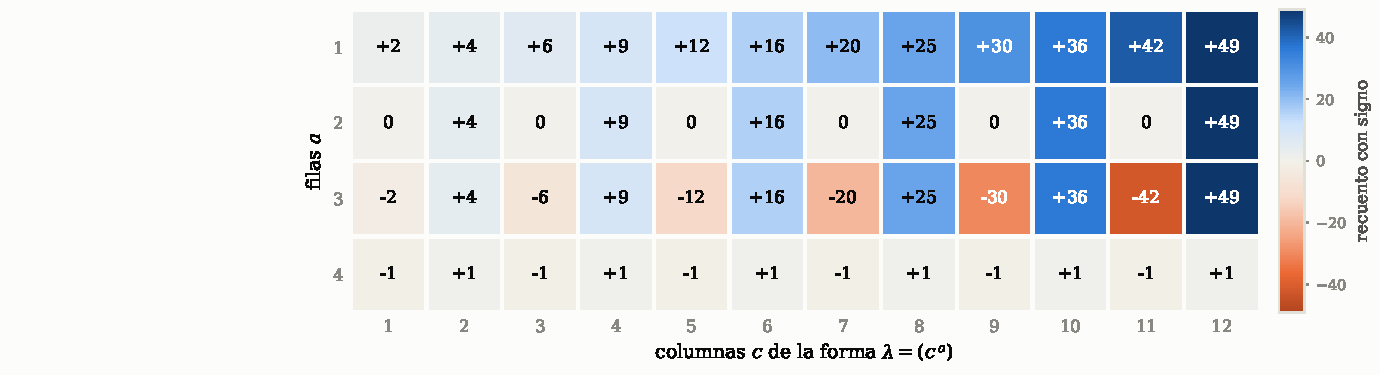
\includegraphics[width=\textwidth]{fig_signed_es.pdf}
\caption{Los recuentos con signo del Ejemplo \ref{ex:boxes}: el valor del Corolario \ref{cor:enum} en
$z=1$ y $t=2$ para las formas rectangulares $\lambda=(c^{\,a})$, esto es la $(-1)$-enumeración de
particiones planas en una caja $a\times(4-a)\times c$. Cada entrada es la forma cerrada
$\varepsilon_\lambda\,d_1d_2d_3/(2t^2)$, contrastada contra una enumeración directa de las tablas. La
fila $a=2$ se anula para $c$ impar y es un cuadrado perfecto para $c$ par.}
\label{fig:signed}
\end{figure}

La literatura de $(-1)$-enumeración calcula tales recuentos con signo, y conviene ser exacto en cómo,
porque la diferencia de aquí es estrecha. Kuperberg \cite{Kup02} pesa los objetos por $\pm1$
directamente. Eisenkölbl \cite{Eis07} especializa $x_i=(-1)^i$ en una identidad de funciones de Schur
del tipo que usó Stanley \cite{Sta86} ---identidad que allí se señala que es también
\cite[Cor.~7.3]{IOTZ06}--- y obtiene la $(-1)$-enumeración de las particiones planas
autocomplementarias con un lado impar. Ciucu y Krattenthaler evalúan los determinantes
correspondientes. En todos ellos el alfabeto es un número y no queda nada libre, que es el único
punto de diferencia: aquí el par recíproco mantiene viva una variable a lo largo del recuento con
signo. Eso lo hace el alfabeto, no un argumento nuestro.

En el mundo de las cintas hay un refinamiento de otra clase, y conviene decir cuál: los polinomios
LLT de Lascoux, Leclerc y Thibon \cite{LLT97} gradúan las tablas de cintas por un estadístico de
spin. Ese $q$ es una graduación añadida y no una letra, y el objeto que gradúa va indexado por una
tupla de formas; el parámetro de aquí es el del propio alfabeto y quien lo transporta es un solo
$s_\lambda$. Los dos refinan cosas distintas, y por eso enunciamos el punto de forma estrecha: es el
par recíproco, y no un estadístico, lo que mantiene viva una variable a través del recuento con
signo.

Una enumeración con signo que tiene fórmula de producto pide una involución que invierta el signo, y
el obstáculo es específico: la involución debe preservar $m_{t+1}-m_{t+2}$, o el parámetro libre no
se transporta, y ni los movimientos de Bender--Knuth ni el intercambio de una sola celda lo hacen.
La construcción de \cite{KumariThesis} de una involución sin puntos fijos que invierte el signo
sobre tablas semiestándar en un alfabeto emparejado por $\pm$, cuyo conjunto fijo son las tablas
embaldosables por dominós, sí tiene la propiedad requerida en su instancia $i=1$: toca solo celdas
que contienen $1$ o $2$, luego preserva $z^{m_3-m_4}$ e invierte $(-1)^{m_2}$. El producto triple
sobre el que tendría que aterrizar es el del Corolario \ref{cor:chars}, que en $t=2$ es sin más un
producto de tres caracteres $\mathfrak{sl}_2$, de modo que la biyección que falta es un enunciado de
Clebsch--Gordan. Esa es una mitad. La
otra es la cancelación a través de la partición del alfabeto, y en $t=2$ concierne a una única
familia de un parámetro. Por \eqref{eq:threestep} más abajo,
\[
s_\lambda(1,-1,z,\zb)=\sum_{\ell(\nu)\le2}s_{\lambda/\nu}(1,-1)\,\chi_{\nu_1-\nu_2}(z),
\]
y una involución que transporte el parámetro debe preservar $k=\nu_1-\nu_2$, porque ese es el índice
del carácter sobre el que se apoya su término. Para $k$ fijo las $\nu$ admisibles son exactamente
$(m+k,m)$ con $m\ge0$, de modo que esa cancelación es un enunciado sobre una sola palabra.

El tamaño de los términos es clásico. El teorema de Littlewood tiene forma sesgada ---$\varphi_t
s_{\lambda/\nu}$ se anula salvo que $\lambda/\nu$ sea embaldosable por $t$-cintas, y en otro caso es
un signo de cinta por un producto sobre el cociente---, debida a Macdonald \cite[p.~91]{Mac95} y
demostrada allí por la misma vía de Jacobi--Trudi que tomamos abajo; el caso en que $\nu$ es el
$t$-núcleo es de Farahat. En $t=2$ y sobre nuestro alfabeto da $\sigma_m\in\{0,\pm1\}$ de inmediato.
Lo que no es clásico es cómo se mueve el signo con $m$, y eso es lo que la involución necesita.

\begin{figure}[t]
\centering
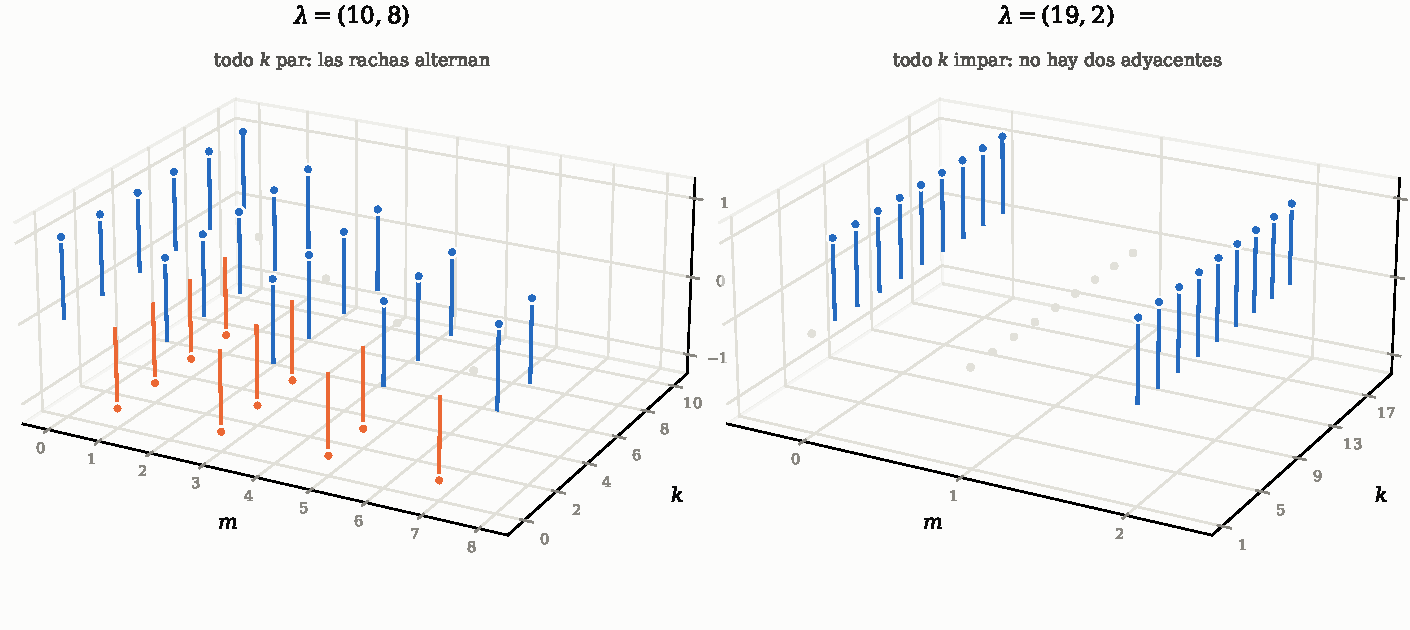
\includegraphics[width=\textwidth]{fig_runs_es.pdf}
\caption{La Proposición \ref{rem:involution}, dibujada. Para cada $k$ las $\nu$ admisibles son la
única familia $(m+k,m)$, y se representa $\sigma_m=s_{\lambda/(m+k,m)}(1,-1)$ frente a $m$ y $k$; los
puntos grises son los ceros. Toda barra tiene altura exactamente $\pm1$, que es la parte (i): los
términos forman un conjunto, luego la cancelación que pide la enumeración es un emparejamiento y no
algo con multiplicidad. A la izquierda todo $k$ es par y el color alterna a lo largo de cada racha,
que es la parte (iii) y lo que hace que $m\leftrightarrow m+1$ invierta el signo; donde una racha
acaba, la acaba un cero. A la derecha todo $k$ es impar y no hay dos términos no nulos contiguos,
que es la parte (ii): las rachas tienen longitud uno y no hay nada que cancelar.}
\label{fig:runs}
\end{figure}

\begin{proposition}[las rachas alternan]\label{rem:involution}
Sean $t=2$ y $k\ge0$, y sea $\sigma_m=s_{\lambda/(m+k,m)}(1,-1)$ para $m\ge0$. Entonces
\begin{enumerate}
\item[\rm(i)] $\sigma_m\in\{0,\pm1\}$ --- esta parte es de Macdonald y no nuestra;
\item[\rm(ii)] si $k$ es impar, no hay dos $\sigma_m$ consecutivos no nulos;
\item[\rm(iii)] si $\sigma_m$ y $\sigma_{m+1}$ son ambos no nulos, entonces
$\sigma_{m+1}=-\sigma_m$.
\end{enumerate}
En consecuencia, emparejar $m$ con $m+1$ dentro de cada racha maximal de $\sigma$ no nulos
consecutivos es una involución que invierte el signo, y $\sum_m\sigma_m$ es el recuento con signo de
las rachas de longitud impar.
\end{proposition}

Las tres partes se ven a la vez en la Figura \ref{fig:runs}: las alturas de las barras son la parte
{\rm(i)}, los huecos del panel impar son la parte {\rm(ii)}, y la alternancia del color a lo largo de
cada racha es la parte {\rm(iii)}.

\begin{proof}
Escribamos $\beta_i=\lambda_i-i$ y $c_j=\nu_j-j$, y tomemos la matriz de Jacobi--Trudi de
$s_{\lambda/\nu}$ con $n\ge\ell(\lambda)$ filas. Como $h_j(1,-1)=1$ para $j\ge0$ par y $0$ en otro
caso,
\begin{equation}\label{eq:betaJT}
M_{ij}=\bigl[\beta_i\ge c_j\bigr]\cdot\bigl[\beta_i\equiv c_j \bmod 2\bigr],\qquad
\sigma_m=\det M .
\end{equation}
El segundo factor dice que la columna $j$ está soportada en las filas de una sola clase de paridad,
la de $c_j$; y como $\beta_1>\dots>\beta_n$, dentro de esa clase el primer factor recorta un
\emph{segmento inicial}. Ordenando las filas por clase de paridad, $M$ queda diagonal por bloques,
de modo que es singular salvo que cada clase lleve tantas columnas como filas tiene, y dentro de una
clase es la escalera $\bigl[\,\text{el rango de }i\text{ en su clase}\le\ell_j\bigr]$ de las
longitudes $\ell_j$. Esa escalera es singular si dos longitudes coinciden o alguna es $0$, y en otro
caso las longitudes son una permutación de $1,\dots,e$ y su determinante es el signo de esa
permutación. Esto da (i), que en este caso es \cite[p.~91]{Mac95}; lo rededucimos porque la forma
$\beta$ \eqref{eq:betaJT} es lo que sostiene (ii) y (iii).

Para $\nu=(m+k,m)$ se tiene $c_1=m+k-1$, $c_2=m-2$ y $c_j=-j$ para $j\ge3$. Luego $c_1-c_2=k+1$, y
pasar de $m$ a $m+1$ sube $c_1$ y $c_2$ en uno y deja las demás columnas quietas: cambian de clase
de paridad exactamente las dos primeras.

Si $k$ es impar entonces $c_1\equiv c_2$, así que las columnas $1$ y $2$ están en la misma clase y
ambas la abandonan. El número de columnas de esa clase cambia en dos mientras que su número de filas
no, de modo que a lo sumo uno de $\sigma_m$, $\sigma_{m+1}$ puede ser no nulo, que es (ii).

Si $k$ es par entonces $c_1\not\equiv c_2$ y las dos columnas intercambian clase. Supongamos que
ambos son no nulos. En la clase de $c_1$ las columnas son la columna $1$ junto con un conjunto de
columnas $j\ge3$ que no se mueve; por (i) las longitudes son una permutación de $1,\dots,e$ antes y
después, y las columnas fijas aportan las mismas a ambas, luego la longitud que trae la columna $2$
es la que se llevó la columna $1$ ---y simétricamente en la otra clase. Cada clase ve por tanto las
mismas longitudes en el mismo orden de columnas, y los dos determinantes de bloque no cambian. Lo
que sí cambia es la baraja que separa las dos clases de columnas: las columnas $1$ y $2$ son
contiguas e intercambian pertenencia, lo que altera el número de inversiones de esa baraja en
exactamente uno. Luego $\sigma_{m+1}=-\sigma_m$, que es (iii).
\end{proof}

\begin{remark}[el signo de aquí es el signo del Teorema \ref{thm:main}]\label{rem:onesign}
Escribamos $\sigma_\nu$ para la permutación de la \S\ref{sec:background} asociada a una partición
$\nu$: la que ordena $\beta$ por clase de residuos, y que la Proposición \ref{rem:sign} coloca
dentro de $\varepsilon_\lambda$. Los términos de la Proposición \ref{rem:involution} son valores de
ese mismo signo. En efecto, $\sigma_m$ se anula salvo que $\core_2(\lambda)=\core_2(\nu)$ y ambas
componentes del $2$-cociente sesgado sean tiras horizontales, y vale
$\sgn(\sigma_\lambda)\sgn(\sigma_\nu)$ cuando no se anula ---siendo la identidad
$\sgn(\sigma_\lambda)\sgn(\sigma_\nu)=(-1)^{\sum_B\mathrm{ht}(B)}$ el signo de cintas de
\cite[p.~91]{Mac95} escrito como signo de ordenación, que es
\cite[Lema 6.3]{KumariThesis}. Las partes {\rm(ii)} y {\rm(iii)} son
entonces un único enunciado sobre $\sigma_\nu$ solo: al pasar $\nu=(m+k,m)$ a $(m+k+1,m+1)$,
$\sgn(\sigma_\nu)$ cambia de signo si $k$ es par y es constante si $k$ es impar. Así que la
permutación que lleva el signo del teorema principal es la permutación que hace alternar la
involución de esta sección; las dos mitades del artículo están firmadas por un mismo objeto.
\end{remark}

El emparejamiento es una biyección de tablas y no solo de términos, que es lo que transporta el
parámetro. Una tabla semiestándar de forma $(a,b)$ en las letras $3,4$ tiene segunda fila $4^{\,b}$
y primera fila $3^{\,p}4^{\,a-p}$ con $b\le p\le a$, de peso $z^{2p-a-b}$; añadirle una primera
columna $\left(\begin{smallmatrix}3\\4\end{smallmatrix}\right)$ la lleva a la tabla de forma
$(a+1,b+1)$ con $p+1$ en lugar de $p$, y $2(p+1)-(a+1)-(b+1)=2p-a-b$, de modo que $m_3-m_4$ se
preserva exactamente. Componer eso con la Proposición \ref{rem:involution} empareja los términos del
Corolario \ref{cor:enum} del modo que la enumeración pide.

Una mitad no es nuestra, y decimos cuál. La Proposición \ref{rem:involution} despacha la cancelación
a través de $\nu$; la cancelación \emph{dentro} de cada $s_{\lambda/\nu}(1,-1)$ es
\cite{KumariThesis}, y las dos encajan. Allí, con $n=1$, el alfabeto es $(x,-x)$ y el peso de un
llenado de dos letras es $(-1)^{c_2}$, que es $\sigma_m$; la involución
\cite[Lema 2.18]{KumariThesis} es libre de puntos fijos sobre los llenados \emph{no cubribles}, de
modo que la suma se reduce a los cubribles, que el \cite[Lema 2.16]{KumariThesis} pone en
correspondencia con tablas de dominó. Lo que hace utilizable la reducción aquí es el
\cite[Lema 2.14]{KumariThesis}: la paridad del número de dominós verticales no depende de la tabla,
luego toda superviviente lleva el mismo signo y $\sigma_m=\pm\#\{\text{llenados cubribles}\}$. Con la
parte (i), eso obliga al recuento a ser a lo sumo uno, así que el conjunto fijo es un único llenado
cuando $\sigma_m\ne0$ y vacío en otro caso ---comprobado directamente sobre las $1134$ formas
sesgadas con a lo sumo cuatro filas y $|\lambda|\le10$, donde los dos recuentos coinciden sin
excepción.

En $t=2$ existe por tanto la involución que la enumeración pide: cancelar dentro de cada $\nu$ por
el \cite[Lema 2.18]{KumariThesis}, emparejar lo que queda a través de $\nu$ por la Proposición
\ref{rem:involution}, y transportar el parámetro con la columna
$\left(\begin{smallmatrix}3\\4\end{smallmatrix}\right)$. Sus puntos fijos son un llenado por cada
racha de longitud impar, y el Corolario \ref{cor:enum} los cuenta. La construcción es de Kumari; el
ensamblaje es nuestro.

%======================================================================
\section{La factorización está aislada}\label{sec:sharp}

Una factorización solo es un resultado si no es especialización de otra conocida, y solo es un
resultado \emph{nítido} si el alfabeto no admite deformación. Eso no lo demostramos en general. Lo
que hacemos es probar cuatro deformaciones de \eqref{eq:object}, y las cuatro destruyen el producto.

La evidencia de esta sección es computacional, y así la etiquetamos: ninguna de (D1)--(D4) es un
teorema, y en particular no demostramos ningún resultado de imposibilidad. Lo que afirmamos es que la
identidad \eqref{eq:main} es falsa para cada alfabeto deformado, cosa que zanja un solo
contraejemplo, y damos recuentos para indicar cuán lejos está de ser cierta.

\begin{itemize}
\item[\rm(D1)] \emph{Más pares recíprocos.} Para
$s_\lambda(\zt,z_1,z_1^{-1},\dots,z_r,z_r^{-1})$
la ley de producto del Teorema \ref{thm:main} ya falla en $r=2$: en el rango calculado los valores
típicos llevan un factor irreducible grande, y los únicos
factores que se observa que se desprendan son binomios en las variables rotadas $z_1z_2$ y $z_1z_2^{-1}$, esto es,
los acoplamientos entre las cargas $u(1)$ de los pares. Lo que sí sobrevive es el \emph{lugar de
anulación}: en $t=2$ sobrevive a todo $r$ y el Teorema \ref{conj:crit} lo determina por completo,
mientras que para $t$ y $r$ arbitrarios el Teorema \ref{thm:suff} da un criterio suficiente uniforme
y la Conjetura \ref{conj:general} es el recíproco. Con esta evidencia el producto parece un accidente
de rango uno y la anulación la parte que generaliza; la primera mitad de esa frase es la Conjetura
\ref{conj:rank2} y sólo la segunda es un teorema.
\item[\rm(D2)] \emph{Más variables en la órbita.} Para
$s_\lambda(X,\zeta X,\dots,\zeta^{t-1}X,z,z^{-1})$ la ley de producto ya falla en $|X|=n=2$. Con $t=2$,
$n=2$ el valor para $\lambda=(2)$ es $(x^2z^2+y^2z^2+z^4+z^2+1)/z^2$, irreducible sobre $\mathbb Q$;
para $\lambda=(2,2)$ es $(x^2+y^2+z^2)(x^2z^2+y^2z^2+1)/z^2$, dos factores en lugar de tres; y para
$\lambda=(3,1)$ es de nuevo irreducible. En cambio, suprimido el par, el mismo alfabeto obedece
\cite[Teorema 2.3]{AK25}: $s_{(2)}(x,y,-x,-y)=x^2+y^2$ y $s_{(2,2)}(x,y,-x,-y)=(x^2+y^2)^2$.
\item[\rm(D3)] \emph{La órbita sustituida por una clase lateral.} Para $\zeta'\zt$ con
$\zeta'=e^{\pi i/t}$, las potencias impares de una raíz $2t$-ésima primitiva de la unidad ---el
torcimiento de \cite[\S3]{AK25}, y para $t$ par el conjunto completo de raíces $2t$-ésimas primitivas
estudiado en \cite{HI24}--- la identidad falla, criterio de anulación incluido.
\item[\rm(D4)] \emph{El par recíproco sustituido por un par libre.} $s_\lambda(\zt,x,y)$ resultó
irreducible en todos los casos que calculamos. No afirmamos nada fuera de ese rango.
\end{itemize}

Recuentos para (D3) y (D4), sobre $t=2,\dots,6$ y $|\lambda|\le10$: la identidad se cumple en los
$600$ casos para \eqref{eq:object}, en $383$ de $600$ para (D3) y en $200$ de $600$ para (D4). El
contraste es por tanto capaz de fallar, que es la razón de citar la primera fila.

Una sola lectura de la demostración explica las cuatro. Partiendo el alfabeto y aplicando el Teorema
\ref{thm:LR} a la mitad congelada se obtiene, para cualquier alfabeto libre $B$,
\begin{equation}\label{eq:threestep}
s_\lambda(\zt\cup B)=\sum_{\nu}s_{\lambda/\nu}(\zt)\,s_\nu(B)=\sum_\nu\varepsilon_\nu\,s_\nu(B),
\qquad \varepsilon_\nu\in\{0,\pm1\},
\end{equation}
siendo los coeficientes signos de cinta: que la evaluación sesgada $s_{\lambda/\nu}(\zt)$ sea $0$ o
un signo de cinta es la forma sesgada del Teorema \ref{thm:LR}, debida a Macdonald
\cite[p.~91]{Mac95}. Ahora bien, $B=(z,z^{-1})$ tiene exactamente dos letras y
son recíprocas, luego $s_\nu(B)=\chi_{\nu_1-\nu_2}(z)$ es un \emph{único} carácter
$\mathfrak{sl}_2$ que depende de una sola diferencia, y la suma corta con signos colapsa. El primer
paso exige que la mitad congelada sea una órbita completa, pues el Teorema \ref{thm:LR} necesita que
las filas toquen cada clase de residuos exactamente; una clase lateral no lo hace, y eso es (D3). El
segundo paso exige que la mitad libre sea exactamente un par recíproco: un par libre tiene
$\det=xy$ y se acopla a las dos cargas centrales, y eso es (D4), mientras que agrandar la mitad libre
---con más pares, o con más variables en la órbita, lo que agranda $\nu$--- hace que $s_\nu(B)$ deje
de ser un único carácter y que la suma deje de colapsar, y eso es (D1) y (D2). \emph{Los cuatro
fallos son una sola condición vista desde cuatro lados.}

\begin{remark}
Equivalentemente: el par recíproco aporta exactamente \emph{un} acoplamiento, el término cruzado
$d_3$, porque $\det=1$ le impide ver por separado las dos cargas centrales. Por eso hay tres factores
y no dos, y las factorizaciones de Ayyer--Kumari, que son productos sobre componentes del cociente
sin acoplamiento alguno, son el caso en que esa aportación está ausente.
\end{remark}

\begin{remark}[una lectura teórico-representacional]\label{rem:twining}
El alfabeto \eqref{eq:object} es cerrado bajo inversión, luego es un elemento del toro de $O(N)$, y
su determinante es $(-1)^{t+1}$. Para $t$ par está por tanto en la componente no identidad, donde un
carácter es un carácter \emph{twining}; la identidad que calcula tales caracteres por plegado se debe
a Jantzen \cite{Jantzen} y, en la forma más próxima a esta, a Kumar--Lusztig--Prasad \cite{KLP},
siendo el álgebra plegada relevante el álgebra órbita. Nuestra restricción es reducible, de modo que
se llega a ella desde la suya con un paso de teoría de Clifford. Lo registramos porque
Ciucu--Krattenthaler \cite{CK09} escribieron que no podían ofrecer una interpretación
teórico-representacional de sus factorizaciones, y \cite{AB19} y \cite{AK25} registran que sigue
faltando; la lectura de aquí es de esa clase. El mecanismo es enteramente suyo, y la demostración
anterior no lo usa. El Lema \ref{lem:AtoSp} concreta esa lectura para el alfabeto \eqref{eq:psir},
donde el álgebra plegada es $C_r$ y el carácter twining es un carácter simpléctico sin más.
\end{remark}

%======================================================================
\section{El lugar de anulación sobrevive a todo $r$}\label{sec:zeros}

Esta sección está más allá de la factorización, y se lee distinto de las siete anteriores. Aquéllas
demuestran enunciados sobre una identidad; ésta pregunta qué queda cuando la identidad ya no está, y
la respuesta es un lugar geométrico y no una fórmula ---demostrado en un sentido para todo $r$, y en
el otro solo hasta donde hemos podido llegar. El cambio de registro es el asunto que cambia, no el
listón.

Por (D1), el producto del Teorema \ref{thm:main} no sobrevive a un segundo par recíproco. Su
\emph{lugar de anulación} sí, y para todo $r$ admite forma cerrada. Escribamos
\begin{equation}\label{eq:psir}
\Psi_r(\lambda)\;:=\;s_\lambda(1,-1,z_1,\bar z_1,\dots,z_r,\bar z_r),\qquad N=2r+2,
\end{equation}
de modo que $\Psi_1$ es \eqref{eq:object} en $t=2$. En toda esta sección $\lambda$ se completa con
ceros hasta tener exactamente $N$ partes, $\beta=\beta(\lambda)$ es su conjunto beta y $E$ y $O$ son
sus entradas pares e impares. Diremos que $\lambda$ es \emph{autocomplementaria de anchura $w$} si
$\lambda_i+\lambda_{N+1-i}=w$ para todo $i$, en cuyo caso $w=\lambda_1+\lambda_N$. Las dos
condiciones que gobiernan la sección son
\begin{equation}\label{eq:branches}
\boxed{\;\;
\underbrace{|E|\in\{0,N\}}_{\text{rama (a)}}
\qquad\qquad
\underbrace{\lambda_i+\lambda_{N+1-i}=w\ \ \text{para todo }i,\ \ w\ \text{impar}}_{\text{rama (b)}}
\;\;}
\end{equation}
La rama (a) dice que el conjunto beta tiene paridad constante; la rama (b), que $\lambda$ es
autocomplementaria de anchura impar.

Enunciamos las cuatro afirmaciones por separado, porque no están demostradas en la misma medida y un
único bicondicional lo ocultaría.

\begin{theorem}[las dos ramas]\label{thm:zeros}
Para todo $r\ge1$ y toda $\lambda$: si se cumple la rama {\rm(a)} o la rama {\rm(b)}, entonces
$\Psi_r(\lambda)=0$.
\end{theorem}

\begin{corollary}\label{cor:sizes}
Si $\lambda$ es autocomplementaria de anchura impar $w$, entonces $|\lambda|=w(r+1)$. En particular
la rama {\rm(b)} solo puede darse para $|\lambda|\equiv r+1 \pmod{2(r+1)}$, y un tamaño fuera de esa
progresión no necesita más comprobación.
\end{corollary}

\begin{proof}
Sumar $\lambda_i+\lambda_{N+1-i}=w$ sobre $i$ cuenta $|\lambda|$ dos veces, luego
$2|\lambda|=wN=w(2r+2)$.
\end{proof}

La progresión se ve en la Figura \ref{fig:zeros}, y merece la pena dejar constancia de que el
enunciado análogo para el lugar entero es falso: la rama {\rm(a)} no está confinada a ella, y por eso
la condición hay que leerla sobre la rama {\rm(b)} sola.

\begin{figure}[!ht]
\centering
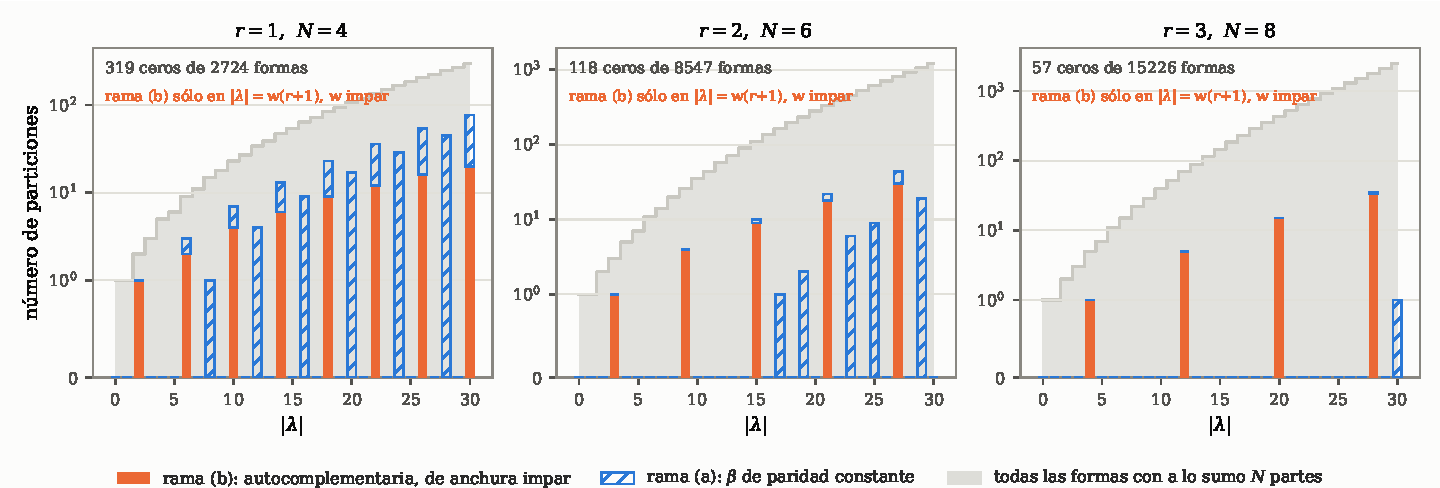
\includegraphics[width=\textwidth]{fig_zeros_es.pdf}
\caption{El lugar de anulación del Teorema \ref{thm:zeros}, contado en lugar de dibujado. Para cada
tamaño $|\lambda|$ las barras dan el número de particiones con a lo sumo $N$ partes que se anulan,
separadas por rama; el escalón sombreado es el número total de formas de ese tamaño, en el mismo eje,
de modo que la rareza del lugar se ve y no se afirma. Los tamaños que llevan la rama (b) son
exactamente los múltiplos $w(r+1)$ con $w$ impar, por el Corolario \ref{cor:sizes}; la rama (a) ocupa
otros tamaños y necesita que el conjunto beta se salte una paridad por completo, razón por la cual
está ausente en $|\lambda|$ pequeño en cuanto $N$ crece.}
\label{fig:zeros}
\end{figure} Conviene dejar constancia de que el enunciado
análogo para todo el lugar de anulación es falso: la rama (a) no está confinada a esa progresión, y
por eso la condición hay que leerla de la rama (b) sola.

\begin{theorem}[un par]\label{thm:r1}
Para $r=1$ vale también el recíproco: $\Psi_1(\lambda)=0$ solo si se cumple {\rm(a)} o {\rm(b)}.
\end{theorem}

\begin{theorem}[dentro del rango de Littlewood]\label{thm:stable}
Para todo $r$ y toda $\lambda$ con $\ell(\lambda)\le N/2$ vale el recíproco. Equivalentemente, en ese
rango $\Psi_r(\lambda)=0$ si y solo si $\lambda=(k^{\,N/2})$ con $k$ impar.
\end{theorem}

\begin{remark}[los rectángulos son donde se detienen los argumentos generales]
Vale la pena advertir que los dos sitios donde falla un argumento general de este artículo son
rectángulos, a dos alturas distintas y por dos razones distintas. A altura $N/2$ un rectángulo impar
es autocomplementario de anchura impar, luego se anula; por el Teorema \ref{thm:stable} son las
únicas formas del rango de Littlewood que lo hacen, y en la demostración son precisamente aquellas
para las que no se puede construir el testigo asociado. A altura completa el objeto no se anula, sino
que degenera en sentido contrario: $s_{(c^{\,N})}(x)=(x_1\cdots x_N)^{c}$ es un monomio, de modo que
sobre cualquier alfabeto $A$ el valor es $\det(A)^{c}$ y de la forma no sobrevive nada ---que con
$t=2$ es el caso {\rm(i)} de la Proposición \ref{prop:rect}, el único allí en el que la paridad de
$c$ no interviene---. Entre ambas alturas el argumento genérico se aplica sin cambios. Los
rectángulos no son una molestia que haya que tratar caso por caso: son el borde de la forma, y cada
uno de los dos extremos rompe una hipótesis distinta ---el primero la existencia de un testigo, el
segundo la no degeneración del triple de intervalos---.
\end{remark}

\begin{theorem}[el criterio en general]\label{conj:crit}
Para todo $r$ y toda $\lambda\in\PP_N$, $\Psi_r(\lambda)=0$ si y solo si se cumple {\rm(a)} o
{\rm(b)}.
\end{theorem}

\noindent Demostrado al final de la \S\ref{sec:zeros}, módulo el Teorema \ref{thm:PvW}.

Los Teoremas \ref{thm:zeros}--\ref{thm:stable} se demuestran en las
\S\S\ref{sec:brancha}--\ref{sec:conv}, y el Teorema \ref{conj:crit} --- el criterio para todo
$r$ --- al final de esta sección, por una vía independiente de los tres. Lo enunciamos aparte por dos
razones. Es el único resultado del artículo que se apoya en algo ajeno, el Teorema
\ref{thm:PvW}; y las dos vías que llevan a él no son la misma vía. La de Littlewood lo reduce, en la
\S\ref{sec:unstable}, a un único enunciado de existencia, y esa reducción no se completa: el rango
$\ell(\lambda)>N/2$ es exactamente donde la regla de restricción deja de aplicarse y, aunque el
Lema \ref{lem:AtoSp} resuelve allí los valores, el enunciado sobre los coeficientes no --- el
certificado que propusimos para él falla, por la Proposición \ref{conj:iso}. El argumento extremal
de las \S\S\ref{sec:extremal} y \ref{sec:rigidity} no entra en ese rango en absoluto: trabaja en
la filtración por grados del numerador y no se cruza jamás con un coeficiente de Littlewood.

Leído sobre el grupo y no sobre el alfabeto, el mismo teorema describe una propiedad de rigidez, y lo
enunciamos aparte porque es la forma en que lo querría alguien de teoría de representaciones. La
traducción no es nuestra ni es nueva: que una representación de $O(N)$ sea estable por $\det$
exactamente cuando su carácter se anula fuera de la componente identidad es elemental, y que eso sea
la condición $m_\nu=m_{\nu^{*}}$ sobre los asociados de Littlewood \cite{Lit50} es clásico. El
corolario reclama por tanto exactamente lo que reclama el Teorema \ref{conj:crit}, y nada más.

\begin{corollary}[rigidez frente al giro por el determinante]\label{cor:dettwist}
Sean $N=2r+2$ y $\lambda\in\PP_N$, y sea $V_\lambda$ el $GL(N)$-módulo polinómico irreducible de peso
máximo $\lambda$. Entonces
\[
V_\lambda\big|_{O(N)}\;\cong\;V_\lambda\big|_{O(N)}\otimes\det
\]
si y solo si $\beta(\lambda)$ tiene paridad constante, o $\lambda$ es autocomplementaria de anchura
impar. Equivalentemente: \eqref{eq:branches} clasifica exactamente los $GL(N)$-módulos polinómicos
irreducibles cuya restricción a $O(N)$ es estable por el carácter del grupo de componentes.
\end{corollary}

\begin{proof}
En característica $0$ un $O(N)$-módulo de dimensión finita es semisimple y queda determinado por su
carácter, así que para $W=V_\lambda|_{O(N)}$ se tiene $W\cong W\otimes\det$ si y solo si
$\chi_W=\chi_{W\otimes\det}$. Esos dos caracteres coinciden automáticamente en la componente
identidad, y en la otra $\chi_{W\otimes\det}=-\chi_W$; luego la condición es que $\chi_W$ se anule en
$O(N)^{-}$. Todo elemento \emph{semisimple} de $O(N)^{-}$ es conjugado a uno de espectro
$(1,-1,z_1^{\pm1},\dots,z_r^{\pm1})$, que es el alfabeto de \eqref{eq:psir}; y como los semisimples
son densos en $O(N)^{-}$ y $\chi_W$ es regular, anularse en ese toro es anularse en toda la
componente. La condición es por tanto $\Psi_r(\lambda)\equiv0$, y el Teorema \ref{conj:crit} es el
criterio. El diccionario entre las dos lecturas es la expansión por asociados de Littlewood, recordada
en la \S\ref{sec:conv}.
\end{proof}

\noindent El crédito se reparte exactamente igual que en el Teorema \ref{conj:crit}, y conviene
repetirlo aquí porque el lenguaje de grupos puede hacer que un enunciado conocido parezca nuevo. Que
las dos familias \eqref{eq:branches} \emph{sean} estables por $\det$ no es nuestro: en el extremo de
la familia, la primera es de Karmakar \cite[Teorema 4.1(A)]{Kar24}, y la segunda es la complementación
sobre la familia de índices de Ayyer y Behrend \cite{AB19}, como recoge \eqref{eq:compl}. Lo que el
Teorema \ref{conj:crit} añade, y es todo lo que añade, es que no hay ninguna más.

\begin{remark}[lo que el núcleo ve, y lo que no]\label{rem:core}
La rama (a) es una condición sobre el núcleo, y sencilla: con un número $N$ fijo de números beta, el
perfil de residuos determina $\core_t(\lambda)$ ---es la coordenada de Garvan--Kim--Stanton
\cite{GKS90}---, de modo que toda condición sobre el perfil lo es sobre el núcleo. No es, sin
embargo, la anulación del núcleo sino su extremo opuesto: en $t=2$ la rama (a) dice
\[
\core_2(\lambda)=(N-1,N-2,\dots,1)\qquad\text{o}\qquad\core_2(\lambda)=(N,N-1,\dots,1),
\]
los dos $2$-núcleos más grandes que admiten $N$ números beta, mientras que
$\core_2(\lambda)=\varnothing$ es el perfil equilibrado. La rama (b) no mueve ni el perfil ni el
núcleo, y por tanto le es invisible. En consecuencia $\core_2$ \emph{no} determina si $\Psi_r$ se
anula, y el testigo más pequeño es el propio núcleo vacío: entre las formas con
$\core_2(\lambda)=\varnothing$ en $r=1$,
\[
(1,1),\ (3,3),\ (2,2,1,1),\ \dots\quad\text{se anulan, y}\quad
\varnothing,\ (2),\ (1^4),\ \dots\quad\text{no,}
\]
y el mismo corte ocurre en $r=2$ y $r=3$, allí también en las clases de núcleo $(1)$, $(2,1)$ y
$(3,2,1)$: sobre los rangos de la \S\ref{sec:verif} hay cinco clases de núcleo que llevan ambos
comportamientos, y el perfil determina el núcleo sin ninguna colisión sobre $260$ perfiles con
$t\le5$. No puede existir, pues, ninguna reformulación del Teorema \ref{thm:zeros} en términos de
$\core_2(\lambda)$: el criterio necesita la forma y no solo su núcleo. Leídos contra el Teorema
\ref{thm:LR}, donde el núcleo vacío es exactamente lo que decide, los dos criterios discrepan en
ambas direcciones ---$(1,1)$ tiene $2$-núcleo vacío y $\Psi_1=0$, mientras que $(1)$ tiene
$2$-núcleo no vacío y $\Psi_1\ne0$.
\end{remark}

La familia de índices de (b) no es nueva: es precisamente la que Ayyer y Behrend destacan
\cite[observación tras el Teo.~3]{AB19}, junto con la obstrucción de paridad que registran allí ---una
partición no puede ser autocomplementaria en un rectángulo $a\times b$ con $a$ y $b$ ambos impares, y
aquí $a=N$ es par, luego el caso admisible es $b=w$ impar. Lo que sus teoremas dicen de esas formas es
que el carácter \emph{factoriza}; allí el alfabeto lleva el punto fijo $+1$ y tiene determinante $+1$.
El nuestro lleva $+1$ y $-1$, y tiene determinante $-1$.

\keybox{Sobre la \emph{misma} familia de formas, el alfabeto de determinante $+1$ hace que el
carácter factorice y el de determinante $-1$ hace que se anule. Una letra separa una factorización de
una aniquilación, y quien decide es el determinante del alfabeto; la identidad \eqref{eq:compl} de
más abajo es donde ocurre la separación.}


\subsection{Rama (a): el alfabeto al cuadrado}\label{sec:brancha}

Esta rama es de Karmakar, en el extremo. \cite[Teorema 4.1(A)]{Kar24} evalúa un carácter de
$\mathrm{GL}(n,\CC)$ en $C_{n-k,k}=(1,\dots,1,-1,\dots,-1)$ y da
$\chi_\lambda(C_{n-k,k})=0$ cuando $\#\eta_0(\lambda)>n-k$, donde su
$\eta_i(\lambda)=\{a\in\lambda+\rho: a\equiv i \bmod 2\}$ es exactamente la partición de
$\beta(\lambda)$ en $E$ y $O$ que usamos aquí; en $k=1$, tras su normalización por el carácter
determinante, eso es la rama (a). El argumento de una línea que sigue se incluye porque es el que
reutiliza el resto de la sección, no porque sea nuevo.

\begin{proof}[Demostración del Teorema \ref{thm:zeros}, rama {\rm(a)}]
Sea $A=\{1,-1,z_1,\bar z_1,\dots\}$. Si $\beta=2\gamma$, entonces
$\det(a^{\beta_j})_{a\in A}=\det\big((a^2)^{\gamma_j}\big)_{a\in A}$, y si $\beta=2\gamma+1$ ocurre lo
mismo tras extraer $\prod_{a\in A}a$. En ambos casos el bialternante factoriza a través del alfabeto
al cuadrado $A^2=\{1,1,z_1^{2},\bar z_1^{2},\dots\}$, en el que la letra $1$ aparece dos veces porque
$1^2=(-1)^2$. Hay dos filas iguales.
\end{proof}

\subsection{Rama (b): una torsión por el determinante, y autodualidad}

\begin{proof}[Demostración del Teorema \ref{thm:zeros}, rama {\rm(b)}]
Sea $\hat\lambda$ el complementario de $\lambda$ en la caja $w\times N$, leído del revés. En
conjuntos beta, $\beta(\hat\lambda)=c-\beta(\lambda)$ recorrido en sentido inverso, con $c=w+N-1$, y
$\hat\lambda$ es el peso máximo de $V_\lambda^{*}\otimes\det^{\,w}$ como $\mathrm{GL}(N)$-módulo. Si
$\lambda=\hat\lambda$, entonces $V_\lambda\cong V_\lambda^{*}\otimes\det^{\,w}$. Restrinjamos a
$O(N)$: toda representación de $O(N)$ es autodual, luego
$V_\lambda|_{O(N)}\cong V_\lambda^{*}|_{O(N)}\cong V_\lambda|_{O(N)}$, de donde
\[
V_\lambda|_{O(N)}\;\cong\;V_\lambda|_{O(N)}\otimes\det^{\,w}.
\]
El alfabeto \eqref{eq:psir} es un elemento del toro de la componente $\det=-1$, así que para $w$
impar la torsión es por $\det$ mismo y el carácter se anula ahí. Para $w$ par, $\det^{\,w}$ es
trivial y el argumento no da nada: por eso la paridad de $w$ no es un adorno.
\end{proof}

Equivalentemente, y esto es el cálculo en lugar de la representación, la identidad de complementación
estándar da
\begin{equation}\label{eq:compl}
s_{\hat\lambda}(A)\;=\;\Big(\textstyle\prod_{a\in A}a\Big)^{c}\,(-1)^{\binom{N}{2}}(-1)^{r}\,
s_\lambda(A)\;=\;(-1)^{c}\,(-1)\,s_\lambda(A),
\end{equation}
usando que $A$ es cerrado por inversión ---$A^{-1}$ es $A$ con los $r$ pares recíprocos
transpuestos, lo que aporta $(-1)^r$--- y que $\prod_{a\in A}a=-1$. Con $c$ par esto se lee
$s_{\hat\lambda}=-s_\lambda$, y una forma autocomplementaria queda aniquilada. La rama (b) del
Teorema \ref{thm:zeros} es por tanto un corolario de dos líneas de una identidad de manual sobre una
familia de índices conocida, y no la reclamamos como nada más. La Figura \ref{fig:involution} dibuja
el emparejamiento que hace la identidad, y a su lado la misma forma con una caja movida, donde el
emparejamiento se rompe; el contenido de la sección es el recíproco.

\subsection{El recíproco}\label{sec:conv}

\begin{figure}[t]
\centering
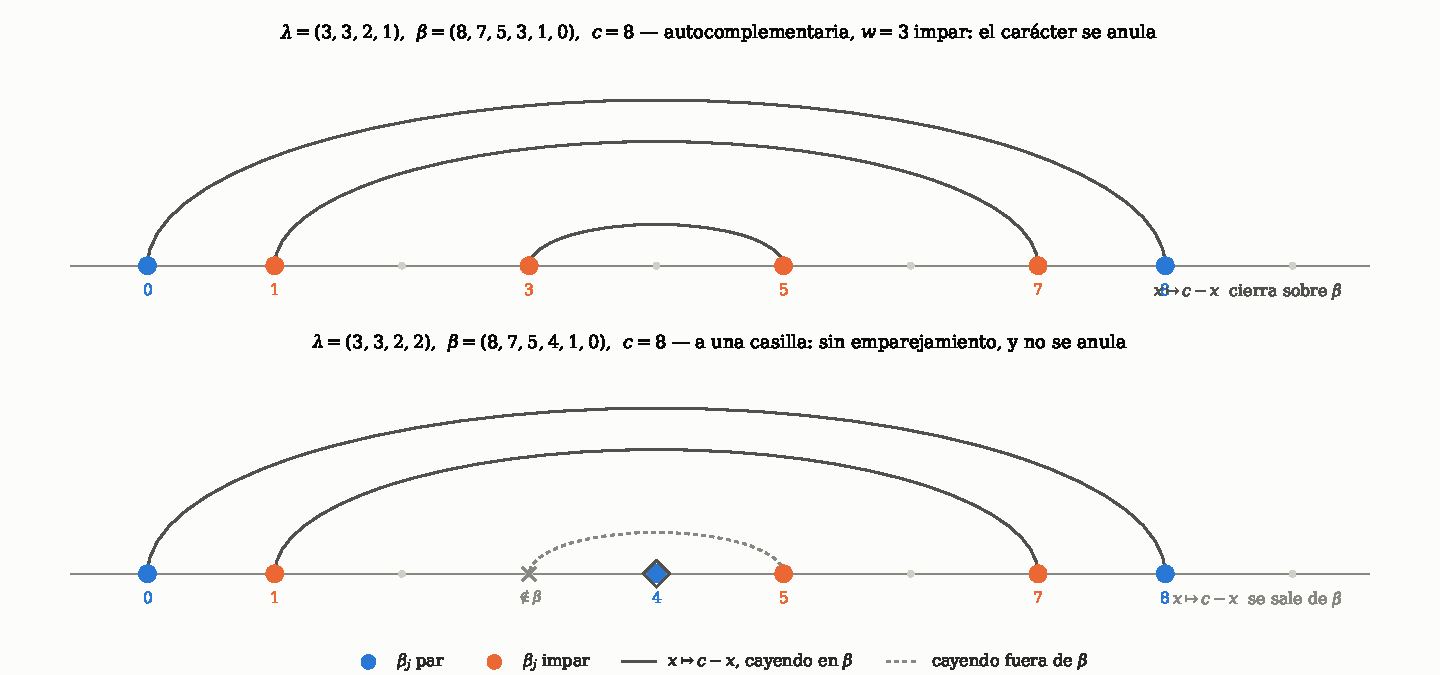
\includegraphics[width=\textwidth]{fig_involution_es.pdf}
\caption{Por qué la autocomplementariedad mata el carácter. Al desarrollar por las dos filas
congeladas quedan términos indexados por pares $(e,o)$ con $e\in E$, $o\in O$, y la reflexión
$x\mapsto c-x$ actúa sobre ellos. Arriba, una forma autocomplementaria de anchura impar: todo arco
cae dentro de $\beta$ y une entradas de igual paridad, porque $c$ es par. Abajo, la misma forma con
una caja movida: el arco $5\mapsto3$ se sale de $\beta$, así que no hay emparejamiento y nada se
cancela. El rombo marca el punto fijo de la reflexión, que no puede darse dentro de un par de
paridades opuestas ---y ésa es la razón de que la involución sea libre.}
\label{fig:involution}
\end{figure}

\begin{proof}[Demostración del Teorema \ref{thm:r1}]
Pongamos $c_\ast=z+\bar z$ y definamos $S_n$ por $S_0=0$, $S_1=1$, $S_{n+1}=c_\ast S_n-S_{n-1}$, de
modo que $\deg_{c_\ast}S_n=n-1$ y $S_{-n}=-S_n$; el valor $S_{-1}=-1$ se usa siempre que
$\beta_N=0$. Como $\Phi_A=(x^2-1)(x^2-c_\ast x+1)$, un polinomio $P$ soportado en $\beta$ es
divisible por $\Phi_A$ exactamente cuando $P(1)=P(-1)=0$ y $P\equiv0$ módulo $x^2-c_\ast x+1$.
Separando $P(\pm1)$ por paridad y reduciendo $x^n\equiv S_nx-S_{n-1}$, la admisibilidad se convierte
en la singularidad de la matriz $4\times4$ con filas $[\beta_j\ \mathrm{par}]$,
$[\beta_j\ \mathrm{impar}]$, $S_{\beta_j}$, $S_{\beta_j-1}$. Desarrollando por las dos filas de
paridad y usando la identidad de d'Ocagne \cite{Doc} para esta recurrencia,
\begin{equation}\label{eq:docagne}
S_bS_{b'-1}-S_{b'}S_{b-1}=-S_{b-b'},
\end{equation}
cada bloque $2\times2$ colapsa a un \emph{único} $S$, indexado por la diferencia de los dos $\beta$
supervivientes. Los $S_n$ distintos tienen grados distintos en $c_\ast$ y son por tanto linealmente
independientes, de modo que la suma con signo se anula solo mediante un emparejamiento exacto de
índices iguales con signos opuestos. El análisis de casos es finito: $|E|\in\{0,4\}$ es la rama (a);
$|E|\in\{1,3\}$ deja tres términos cuyos índices son las tres diferencias dos a dos de un conjunto de
tres elementos y por tanto siempre distintas, así que no existe emparejamiento y el valor no es nulo;
y para $|E|=2$ hay cuatro términos y tres emparejamientos perfectos, y se comprueban los seis
patrones de paridad directamente. Para $E=\{\beta_1,\beta_4\}$ y para $E=\{\beta_2,\beta_3\}$ solo
uno de los tres emparejamientos está disponible, e impone la única condición
$\beta_1+\beta_4=\beta_2+\beta_3$, que es la rama (b); para los cuatro patrones restantes, cada uno
de los tres emparejamientos obliga a dos entradas distintas de $\beta$ a coincidir, así que ninguno
está disponible y el valor no es nulo.
\end{proof}

La identidad \eqref{eq:docagne} es clásica. El colapso que produce es un accidente de rango uno: dos
letras admiten un solo hueco, luego $s_{(m,n)}(z,\bar z)=S_{m-n+1}$ depende solo de ese hueco. No hay
análogo de rango $r$. Lo habría si existiera una forma cerrada de $s_\mu$ en alfabeto recíproco para
\emph{toda} $\mu$; \cite{CK09} la dan para formas rectangulares y \cite{AB19} para las
autocomplementarias, y nadie en general.

Para $r$ general usamos asociados, en el sentido de Littlewood \cite{Lit50}.
En el coset $\det=-1$, la relación $[\nu^{*}]=[\nu]\otimes\det$ da
$\Psi_r=\sum_\nu\big(m_\nu-m_{\nu^{*}}\big)\chi_{[\nu]}$, luego $\Psi_r=0$ si y solo si
$m_\nu(\lambda)=m_{\nu^{*}}(\lambda)$ para toda $\nu$; equivalentemente, si y solo si
$V_\lambda|_{O(N)}$ es invariante por $\det$. Esa equivalencia es el diccionario a través del cual se
lee el Corolario \ref{cor:dettwist}, y es lo que convierte el criterio en un enunciado sobre módulos
y no sobre un alfabeto. Un testigo es por tanto una sola $\nu$ con
$m_\nu\ne m_{\nu^{*}}$, y se puede construir.

El \cite[Teorema 4.1]{Kar24} de Karmakar determina el valor en el extremo $z_i=1$, que es un elemento
de orden dos: el caso (A) es la rama (a), el caso (B) es una dimensión no nula, y el caso (C) deja una
suma alternante de productos de dimensiones sin criterio de anulación asociado. La rama (b) vive en
ese caso (C), de modo que el teorema siguiente no es consecuencia suya. Y el caso (B) tampoco ayuda
más al crecer $r$: con $k=1$ pide que $N-1$ de los $N$ números beta compartan paridad, y la forma más
pequeña que lo hace es la escalera $(2r-1,2r-2,\dots,1)$, de tamaño $r(2r-1)$, así que sobre un rango
fijo de $|\lambda|$ su caso de no anulación sólo se ve para $r$ pequeño --- su resultado es más
afilado exactamente donde el nuestro es más fácil. Lo que conecta el extremo con
la curva es la rigidez, y la rigidez es un enunciado sobre nuestro objeto y no sobre el elemento de
orden dos: sobre los rangos de la \S\ref{sec:verif} se cumple en $\ell(\lambda)\le N/2$ sin excepción
y falla fuera, que es la Observación \ref{rem:rankone}.

\begin{proof}[Demostración del Teorema \ref{thm:stable}]
La rama (a) no puede darse: con $\ell(\lambda)\le N/2$ se anulan al menos dos partes finales, luego
$\beta$ contiene dos enteros consecutivos. En el rango de Littlewood,
$m_\nu(\lambda)=\sum_{\beta'\ \mathrm{par}}c^{\lambda}_{\nu\beta'}$, y el término
$\beta'=\emptyset$ da $m_\mu\ge1$ para toda $\mu\subseteq\lambda$. Tomemos $\mu$ así. Si
$\ell(\lambda)<N/2$, tomamos $\mu=\lambda$: entonces
$\ell(\lambda^{*})=N-\ell(\lambda)>\ell(\lambda)$, luego $\lambda^{*}\not\subseteq\lambda$ y
$m_{\lambda^{*}}=0\ne m_\lambda$. Si $\ell(\lambda)=N/2$ y $\lambda_{N/2}$ es par, tomamos
$\mu=(\lambda_1,\dots,\lambda_{N/2-1})$; entonces $\beta'=(\lambda_{N/2})$ es par, $\lambda/\mu$ es
una tira horizontal y $m_\mu\ge1$ con $\ell(\mu)<N/2$, así que se aplica a $\mu$ el cálculo anterior.
Si $\ell(\lambda)=N/2$ y $\lambda$ no es un rectángulo, sea $j\le N/2-1$ el mayor índice con
$\lambda_j>\lambda_{j+1}$ y quitemos la última fila y además una caja de la fila $j$; entonces
$\beta'=(\lambda_{N/2}+1)$ es par y $\lambda_j\ge\lambda_{N/2}+1$ mantiene $\lambda/\mu$ como tira
horizontal. Un rectángulo par $\lambda=(k^{\,N/2})$ ya lo cubre la segunda construcción, de modo que
el único caso que queda es $k$ impar, donde no está disponible ninguna de las dos construcciones
---y eso es la rama {\rm(b)}---.
\end{proof}

\subsection{Fuera del rango de Littlewood}\label{sec:unstable}

Para $\ell(\lambda)>N/2$ la regla de restricción adquiere etiquetas no estándar, y las reglas de
modificación que las reducen son las de King \cite{King71}; Koike y Terada
\cite{KT87} registran que la especialización de tipo $D$ manda un carácter universal a
$0$ o a $\pm$ otro, y Fauser, Jarvis, King y Wybourne observan que más allá de los dos casos clásicos
\emph{``la teoría general, con infinitos casos, requiere un formalismo aún no disponible''}
\cite[\S4]{FJKW05}. Extensiones de la regla de Littlewood a todos los parámetros sí existen para los
dos casos clásicos --- las reglas de modificación de Newell \cite{New51}, Sundaram \cite{Sun90} en el
caso simpléctico, la demostración de Gavarini por álgebras de Brauer \cite{Gav99}, y Enright y
Willenbring \cite{EW04}, cuyo Teorema 4 da la multiplicidad como una suma alternante sobre el grupo de
Weyl que en casos favorables colapsa a una diferencia de dos coeficientes de Littlewood
\cite[\S7.11]{EW04}. Esa observación de \cite{FJKW05} es de 2005, y conviene dejar escrito que el
hueco que señala se ha llenado desde entonces por el lado que necesitamos: Frohmader
\cite{Frohmader} da reglas de ramificación combinatorias para $GL_n\downarrow O_n$ y
$GL_{2n}\downarrow Sp_{2n}$ que generalizan las reglas de restricción de Littlewood y son, en sus
palabras, \emph{«válidas para todos los parámetros, es decir, no hay restricciones de rango
estable»}; la multiplicidad pasa a ser una suma de coeficientes de Littlewood--Richardson
generalizados $c^{\lambda}_{\mu\nu}(O_n)$ leídos de condiciones de bandera sobre tablas de
Littlewood--Richardson ordinarias, sin ninguna regla de modificación. No la usamos abajo, y decimos
por qué en un momento; pero es el instrumento natural para la única pregunta que esta sección deja
abierta, y volvemos a ella en el Problema \ref{prob:instrument}.

La ruta de aquí es la dual: mantener universales los coeficientes, que lo son en
todo rango, y trasladar toda la dependencia del rango a los valores, donde un solo lema la liquida.
Sobre este alfabeto no hace falta formalismo alguno para las etiquetas, y la razón es que los valores
no son valores de tipo $D$.

Añadir una letra $c$ a un alfabeto actúa sobre el anillo de funciones simétricas por
$p_k\mapsto p_k+c^k$; escribimos $\iota_c$ para ese homomorfismo. De la función generatriz de las
funciones simétricas homogéneas completas, $h_m(W,c)-c\,h_{m-1}(W,c)=h_m(W)$ para todo $m$.

\begin{lemma}[el alfabeto es simpléctico]\label{lem:AtoSp}
$\iota_{-1}\iota_{1}\,o_\nu=sp_\nu$ para toda partición $\nu$, como identidad entre caracteres
\emph{universales} de Koike--Terada en $\Lambda$. En particular, para el alfabeto
\eqref{eq:psir},
\begin{equation}\label{eq:AtoSp}
o_\nu(A)\;=\;sp_\nu(z_1,\dots,z_r)
\end{equation}
sin hipótesis sobre $\ell(\nu)$ y sin signo. Para $\ell(\nu)>r$ el miembro derecho es ese
carácter universal especializado a $r$ variables, no un carácter irreducible de $Sp(2r)$; son las
reglas de modificación de más abajo las que lo pliegan sobre uno.
\end{lemma}

\begin{proof}
Ambos pasos son de Ayyer y Kumari, y ambos son la misma manipulación: la recurrencia convierte las
operaciones de columna $C_j\to C_j-c\,C_{j-1}$, aplicadas para $j=n,\dots,2$ en ese orden, en un
cambio de tipo de carácter, y operaciones de esa forma dejan invariante un determinante. Con $c=1$
llevan el determinante que define $o_\nu$, evaluado en $(W,1)$, al del carácter universal ortogonal
impar $so_\nu$ sobre $W$, que es el diccionario de Koike y Terada en la forma
$so_\nu(X)=o_\nu(X,\bar X,1,0,0,\dots)$ \cite[(2.13)]{AK25}. Con $c=-1$, donde la recurrencia es
\cite[Proposición 2.1]{AK25} y las operaciones se leen $C_j\to C_j+C_{j-1}$, llevan $so_\nu$ a
$sp_\nu$, que es \cite[Lema 3.2]{AK25}. Componiendo se obtiene el primer enunciado, y evaluándolo en
el alfabeto recíproco $(z_1,\dots,z_r)$ se obtiene \eqref{eq:AtoSp}.
\end{proof}

\noindent Como $\nu'_1=\ell(\nu)$, la tricotomía sobre $\nu'_1$ frente a $N/2=r+1$ es una tricotomía
sobre la longitud de $\nu$ frente al rango de $Sp(2r)$, y los tres hechos que necesitamos son
entonces las reglas de modificación simplécticas clásicas --- uno de los dos casos que
\cite{FJKW05} exceptúa --- leídas a través de \eqref{eq:AtoSp}: $o_\nu(A)=0$ cuando $\ell(\nu)=r+1$,
la anulación de un carácter simpléctico una fila más allá de su rango; $o_\nu(A)=\pm o_{\nu^{*}}(A)$
cuando $\ell(\nu)>r+1$, la regla de King plegando la etiqueta sobre una dominante; y lo mismo para
$\nu$ no estándar, que por el Lema \ref{lem:nonstd} son exactamente las altas. La expansión
$s_\lambda=\sum_\nu c_\nu o_\nu$, con $c_\nu=\sum_{\beta'\ \mathrm{par}}c^{\lambda}_{\nu\beta'}$, es
una identidad de funciones simétricas y vale en todo rango; especializarla en \eqref{eq:psir} deja
por tanto todo término sobre $\{o_\mu(A):\ell(\mu)\le r\}$, que por \eqref{eq:AtoSp} es el conjunto de
los caracteres irreducibles de $Sp(2r)$ y es por ello linealmente independiente. La Figura
\ref{fig:reduction} clasifica las etiquetas en las cuatro clases que describe este párrafo y calcula
$o_\nu(A)$ en cada una, de modo que puede verse que la reducción aterriza donde se afirma. Luego

\begin{figure}[!ht]
\centering
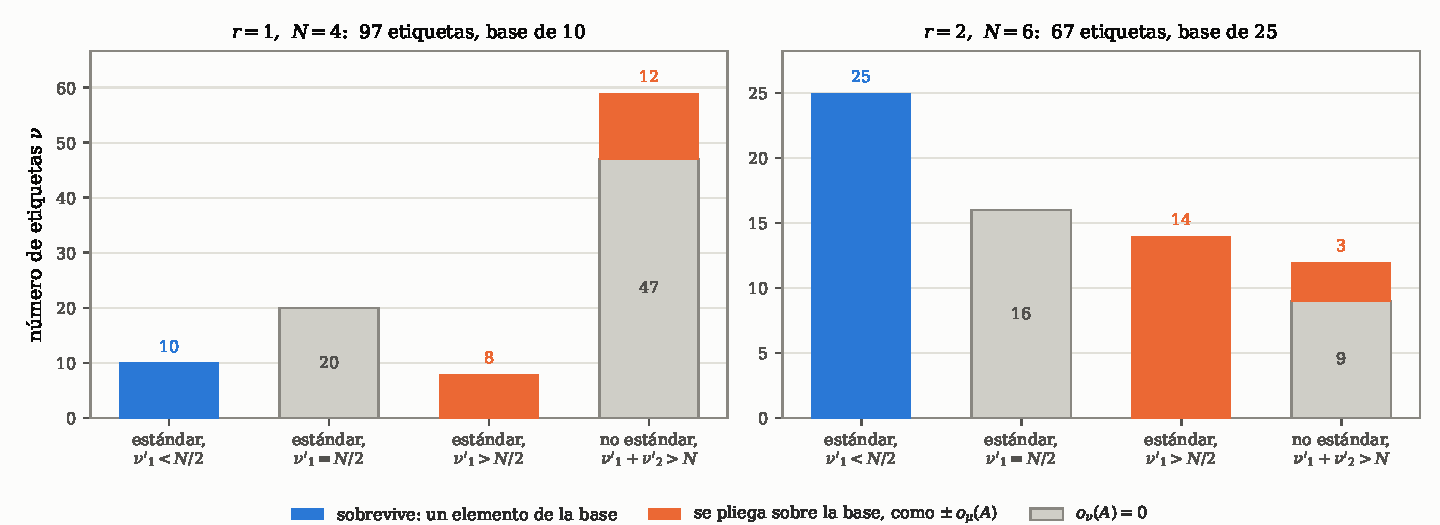
\includegraphics[width=\textwidth]{fig_reduction_es.pdf}
\caption{La reducción del Lema \ref{lem:AtoSp}, dibujada. Cada etiqueta
$\nu$ que aparece en $s_\lambda=\sum_\nu c_\nu o_\nu$ se coloca en una de cuatro clases y se calcula
su valor $o_\nu(A)$. Las etiquetas autoasociadas se anulan, todas ellas; las estándar con
$\nu'_1>N/2$ se pliegan sobre la base como $\pm o_{\mu}(A)$; las no estándar o se anulan o se pliegan
sobre un único elemento de la base con coeficiente $\pm1$. Por \eqref{eq:AtoSp} estas tres son las
reglas de modificación simplécticas disfrazadas, con las clases cortadas por $\ell(\nu)$ frente al
rango $r$; la figura se calculó antes de advertirlo y se deja tal cual. Todo aterriza en la base
independiente $\{o_\mu(A):\ell(\mu)\le r\}$, que es lo que convierte la anulación en la condición
finita \eqref{eq:Cmu}. Las alturas de las barras son recuentos de etiquetas sobre el rango en que se
calculó cada panel, menor que el de la fila correspondiente de la \S\ref{sec:verif}; lo que la imagen
cuenta es la clasificación, no el recuento.}
\label{fig:reduction}
\end{figure}
\begin{equation}\label{eq:Cmu}
\Psi_r(\lambda)=\sum_{\ell(\mu)\le r}C_\mu(\lambda)\,o_\mu(A),
\qquad
\Psi_r(\lambda)=0\iff C_\mu(\lambda)=0\ \text{para toda }\mu,
\end{equation}
donde $C_\mu=c_\mu\pm c_{\mu^{*}}+\sum\pm c_\nu$, sumando sobre las $\nu$ no estándar que se reducen
a $\mu$. La reducción se hace en dos pasos y no en uno: la mayoría de las etiquetas no estándar se
emparejan con una asociada dentro del rango, mientras que $21$ de ellas --- $18$ con $r=1$ y $3$ con
$r=2$ --- no tienen asociada en rango y se reducen aparte, cayendo cada una en el span de los valores
estándar con coeficientes enteros.

Habíamos calculado los tres hechos antes de localizarlos, y dejamos constancia del cálculo porque es
lo que dibuja la figura de abajo: \texttt{sec8\_derivation.sage} comprueba \eqref{eq:AtoSp}
directamente para todo $|\nu|\le8$, confirma que las etiquetas de longitud $r+1$ se anulan y que las
más largas se pliegan sobre la base con un signo, y verifica la independencia como un cálculo de
rango, con $r=1,2,3$. Un control que tenía que dispararse: $\iota_1 o_\nu$ y $\iota_{-1}o_\nu$
coinciden con $sp_\nu$ sólo para $\nu=\varnothing$, de modo que hacen falta las dos letras y
\eqref{eq:AtoSp} es un enunciado sobre el par recíproco y no sobre ninguna de las dos por separado.
\texttt{sec8\_formulas.sage} comprueba la demostración y no el enunciado --- la recurrencia con cuatro
valores de $c$, los dos determinantes que definen los caracteres frente a una implementación
independiente, y las operaciones de columna entrada por entrada. Esta última comprobación se ganó el
sueldo: un borrador previo de la demostración escribía $C_j\to C_j+C_{j-1}$ con $c=1$, que es el signo
que \cite[Lema 3.2]{AK25} usa para su propio paso con $c=-1$.

Las etiquetas no estándar, que son aquí toda la obstrucción, no pueden ser pequeñas:

\begin{lemma}[las etiquetas no estándar son grandes]\label{lem:nonstd}
Toda $\nu$ no estándar que aparezca en el desarrollo cumple $|\nu|\ge N+1=2r+3$. En consecuencia, si
$|\lambda|\le2r+2$ ninguna etiqueta no estándar está contenida en $\lambda$, la última suma de $C_\mu$
queda vacía y $C_\mu(\lambda)=c_\mu(\lambda)\pm c_{\mu^{*}}(\lambda)$ --- sin hipótesis alguna sobre
$\ell(\lambda)$, luego también fuera del rango de Littlewood.
\end{lemma}

\begin{proof}
Como $c^{\lambda}_{\nu\beta'}=0$ salvo si $\nu\subseteq\lambda$, solo aparecen etiquetas con
$\ell(\nu)\le\ell(\lambda)\le N$. Ser no estándar significa $\nu'_1+\nu'_2>N$. Si $\nu$ tuviera una
sola columna sería $\nu'_2=0$ y haría falta $\nu'_1=\ell(\nu)>N$, que queda excluido; luego
$\nu'_2\ge1$ y $|\nu|\ge\nu'_1+\nu'_2>N=2r+2$. Así que una $\nu$ no estándar solo puede contribuir
cuando $|\lambda|\ge|\nu|\ge2r+3$.
\end{proof}

\noindent Como $\ell(\lambda)>N/2$ obliga a $|\lambda|\ge r+2$, el Lema \ref{lem:nonstd} resuelve de
golpe la franja $r+2\le|\lambda|\le2r+2$ del rango inestable: ahí la regla de Littlewood se aplica
literalmente y el recíproco se sigue por el argumento del Teorema \ref{thm:stable}. Lo que esta ruta
todavía tiene que cruzar es $|\lambda|>2r+2$.


Dos hechos exactos acotan a los competidores. Primero, $\ell(\mu^{*})=N-\ell(\mu)$, de modo que
$\ell(\mu)\le N-1-\ell(\lambda)$ obliga a $\mu^{*}\not\subseteq\lambda$ y a $c_{\mu^{*}}=0$. Segundo,
una $\nu$ no estándar cumple $\nu'_1+\nu'_2>N$ con $\nu'_2\le\nu'_1$, luego $2\ell(\nu)>N$ y
$\ell(\nu)\ge r+2$; en particular, en el rango de Littlewood ninguna etiqueta no estándar cabe dentro
de $\lambda$. Llamemos $\mu$ \emph{aislante} para $\lambda$ si exactamente una de las etiquetas que
alimentan $C_\mu$ está contenida en $\lambda$; entonces $C_\mu=\pm c_\nu\ne0$ y
$\Psi_r(\lambda)\ne0$. Lo que la ruta pide ahí es un único enunciado de existencia ---abierto como
enunciado de existencia, aunque no como teorema, pues el Teorema \ref{conj:crit} no pasa por él---.

\begin{proposition}[el testigo aislante no siempre existe]\label{conj:iso}
En $r=2$ la forma $\lambda=(5,5,2,1)$ cumple $\Psi_2(\lambda)\ne0$ y no es de tipo {\rm(a)} ni de
tipo {\rm(b)}, y ninguna $\mu$ es aislante para ella: toda $\mu$ cuyo $C_\mu$ tenga un contribuyente
no nulo dentro de $\lambda$ tiene exactamente dos, a saber $\mu$ y su asociado $\mu^{*}$.
\end{proposition}

Habíamos propuesto el testigo aislante como la vía hacia el Teorema \ref{conj:crit}, y no llega. La
razón se lee en el lema de aislamiento: exige $\ell(\mu)\le N-1-\ell(\lambda)$, lo que con
$\ell(\lambda)=4$ y $N=6$ deja solo $\mu$ de una fila, y una forma tan ancha como $(5,5,2,1)$
contiene a todos los asociados. Sobre $r=2$ y $|\lambda|\le14$ hay once formas así, la menor esta
misma, y ninguna por debajo de $|\lambda|=13$, que es la razón de que el certificado parezca sólido
en rangos pequeños. El Teorema \ref{conj:crit} en sí queda intacto ---afirma que los $C_\mu$ se
anulan, no que exista un certificado--- pero esta vía hacia él queda cerrada. La que sí llega, la
\S\ref{sec:rigidity}, no pasa por el rango de Littlewood, y por eso el fallo de aquí cuesta la
explicación y no el teorema.

El mecanismo alcanza mucho: en $r=2$ y $|\lambda|\le14$, $227$ de las $238$ formas inestables no
nulas llevan un testigo aislante demostrado. Y alcanza más de lo que el hecho (ii) permite por sí
solo ---el mínimo real de $\ell(\nu)$ sobre las $\nu$ no estándar con $o_\nu(A)\ne0$ es allí $5$,
frente al $r+2=4$ que da la cota. Lo que lo derrota es la anchura y no la altura: la base de
\eqref{eq:Cmu} crece con $r$ y las etiquetas competidoras están obligadas a ser altas, así que
leíamos el aislamiento como algo que se facilita con $r$, y a lo largo del eje de la altura así es;
el residuo vive donde $\lambda$ es lo bastante ancha para tragarse los asociados. Esa lectura predice
dónde el residuo \emph{no} está: en $r=3$ el lema de aislamiento permite $\ell(\mu)\le7-\ell(\lambda)$,
de modo que una forma tiene que ser más ancha que en $r=2$ antes de poder tragarse todos los
asociados, y los mismos tamaños deberían salir limpios. Y salen ---sobre $r=3$ y $|\lambda|\le13$ las
$149$ formas inestables no nulas llevan todas un testigo demostrado y el residuo es vacío---, lo cual
es un control sobre la explicación, no un paso hacia el Teorema \ref{conj:crit}. En $r=1$ la
cuestión no se plantea, pues ese caso lo resuelve por separado el Teorema \ref{thm:r1}.

La herramienta a la que uno acude primero no encaja. La saturación, en la forma de panal de Knutson
y Tao \cite{KT99}, decide cuándo un coeficiente de Littlewood--Richardson aislado es positivo, y todo
competidor que alimenta a $C_\mu$ lo es en cuanto su etiqueta cabe dentro de $\lambda$. Lo que un
$\mu$ aislante pide no es positividad sino \emph{aislamiento}: que exactamente uno de ellos quepa. La
positividad es lo que vuelve difícil la pregunta, no lo que la responde, y no conocemos herramienta
alguna dirigida a la segunda.

\begin{figure}[t]
\centering
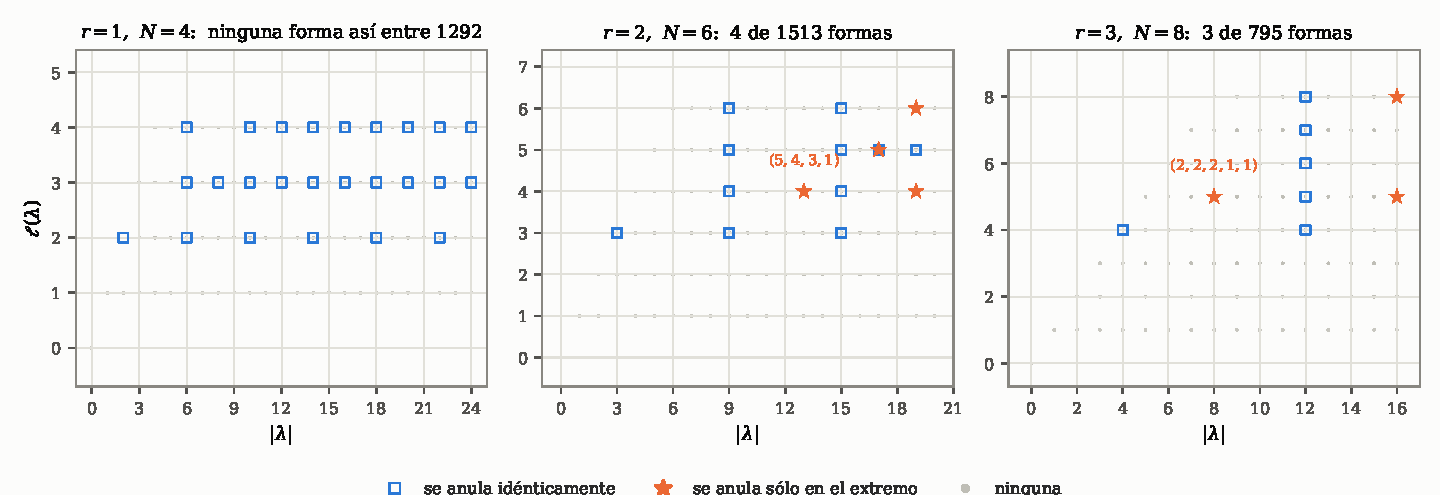
\includegraphics[width=\textwidth]{fig_phase_es.pdf}
\caption{Dónde deja de ser típico un solo par recíproco. Cada partición con a lo sumo $N$ partes es un
punto en $(|\lambda|,\ell(\lambda))$; la clase dibujada con estrella es la que se anula en el extremo
$z_i=1$ sin anularse idénticamente, y es todo el contenido de la imagen; cada panel nombra a su
miembro más pequeño y la Observación \ref{rem:rankone} enumera los demás.
Los paneles cubren $|\lambda|\le24$, $20$ y $16$ respectivamente. En $r=1$ la clase
está vacía sobre las $1292$ formas del rango, porque allí el objeto es $\pm$ un carácter genuino y su
valor en la identidad es una dimensión. A partir de $r=2$ aparecen ejemplos genuinamente virtuales y
la clase deja de estar vacía ---no que toda forma lo sea: el Cuadro \ref{tab:virtual} cuenta las dos
cosas---. Véase la Observación \ref{rem:rankone}.}
\label{fig:phase}
\end{figure}

\begin{remark}[el accidente de rango uno, y dónde se separan los dos rangos]\label{rem:rankone}
En $r=1$ el objeto es $\pm$ un carácter genuino, así que su valor en la identidad es una dimensión y
$\Psi_1(\lambda)\equiv0$ si y solo si $\Psi_1(\lambda)|_{z=1}=0$. En $r\ge2$ la expansión plegada
\emph{puede} ser genuinamente virtual ---no que lo sea siempre, y el Cuadro \ref{tab:virtual} cuenta
las dos columnas---, y basta una forma en que lo sea para romper esa equivalencia:
$\lambda=(5,4,3,1)$ con $r=2$ cumple
$\Psi_2(\lambda)\ne0$ y $\Psi_2(\lambda)|_{z_1=z_2=1}=0$. La Figura \ref{fig:virtual} muestra
los dos regímenes uno al lado del otro, sobre dos formas que difieren en una sola casilla. Sobre los rangos de la Figura
\ref{fig:phase}, la clase de tales formas está vacía en $r=1$ a lo largo de $1292$ particiones; en
$r=2$ consta de las cuatro formas $(5,4,3,1)$, $(5,5,4,2,1)$, $(10,5,3,1)$ y $(6,5,4,2,1,1)$, y en
$r=3$ de las tres formas $(2,2,2,1,1)$, $(5,5,4,1,1)$ y $(3,3,3,2,2,1,1,1)$; es delgada, pero no está
vacía, y un solo contraejemplo es todo lo que la equivalencia puede soportar. La implicación que sí
sobrevive ---anulación exacta $\Rightarrow$ anulación en el extremo--- es lo que hace del extremo un
tamiz válido y nada más. Por eso los resultados calculados en elementos de orden dos ---Karmakar
\cite{Kar24} a lo largo de toda esa familia, Eisenkölbl \cite{Eis07} en el equilibrado
$x_i=(-1)^i$--- hablan de un punto y no de la curva, y por eso el
Teorema \ref{thm:zeros} no es un corolario suyo para $r\ge2$.
\end{remark}

Conviene ponerle un número a lo que el tamiz del extremo deja escapar, porque el enunciado
cualitativo se lee con facilidad como una corrección pequeña. Sobre los rangos de la Figura
\ref{fig:phase}, el contraste $\Psi_r(\lambda)|_{z_i=1}=0$ señala $143$ formas en $r=1$, $22$ en $r=2$
y $9$ en $r=3$; de ellas, $0$, $4$ y $3$ respectivamente no se anulan idénticamente. El tamiz es
entonces exacto con un solo par, y la proporción de sus veredictos que resultan espurios crece con el
número de pares: $0\%$, $18\%$, $33\%$ sobre estos rangos. Un cálculo en el extremo es un filtro que
nunca se salta un cero genuino, y pasado un par no es nada más que eso. El caso de rango uno con
$t=2$, donde el tamiz resulta exacto porque el objeto es un carácter genuino, se trató aparte en
\cite{Mar26}; el alfabeto \eqref{eq:object} surgió allí, en un cálculo de líneas de Wilson sobre un
orbifold, y de ahí que el $-1$ aparezca como letra y no como elección.

Vale la pena separar la razón de que los dos rangos de $\ell(\lambda)$ se comporten de forma tan
distinta del mecanismo que lo demuestra. La regla de Littlewood dice qué etiquetas $\nu$ pueden
aparecer, y $\ell(\lambda)\le N/2$ es exactamente la condición bajo la cual las no estándar no caben
dentro de $\lambda$. El Lema \ref{lem:nonstd} dice que la obstrucción la gobierna $|\lambda|$ además
de $\ell(\lambda)$, así que la imagen honesta no es de dos rangos sino de una región: \emph{esta
ruta} alcanza el recíproco allí donde $\ell(\lambda)\le N/2$ o bien $|\lambda|\le2r+2$, y fuera de la
unión de ambas no llega ---el testigo aislante cubre casi todo lo que queda pero demostrablemente no
todo, por la Proposición \ref{conj:iso}---. El recíproco no está abierto ahí. El Teorema
\ref{conj:crit} lo resuelve para todo $r$ y toda $\lambda$ por el argumento extremal de las
\S\S\ref{sec:extremal}--\ref{sec:rigidity}, que no entra en este rango en absoluto. Lo que la región
marca es dónde deja de explicar la reducción de Littlewood, no dónde deja de valer el teorema.

%======================================================================
% ---- v2_new_subsections_es.tex ----
\subsection{El criterio en \texorpdfstring{$t=2$}{t=2}: el argumento extremal}\label{sec:extremal}

En esta subsección y en las dos siguientes, $t\ge2$ y $r\ge1$ son arbitrarios y
\[
  N:=t+2r,\qquad
  \Phi_{t,r}(\lambda;z):=s_\lambda\bigl(\zt,\,z_1,\zb_1,\dots,z_r,\zb_r\bigr),
\]
de modo que $\Phi_{t,1}$ es \eqref{eq:object} y $\Phi_{2,r}=\Psi_r$. El beta-conjunto, los recuentos
de residuos $n_i$ y la indexación de las columnas son los de la \S\ref{sec:background}; $\lambda\in\PP_N$ y
$\beta_1>\dots>\beta_N\ge0$. Escribimos
\[
  \mathcal{E}=\{i:n_i(\lambda)\ge2\},\qquad e=|\mathcal{E}|,\qquad
  \mathcal{S}=\{\beta_j:\beta_j\equiv i\ (t)\ \text{para algún } i\in\mathcal{E}\}
\]
para las \emph{clases de exceso} y los \emph{valores de exceso}. Como las $t-e$ clases restantes son
unitarias, \eqref{eq:excess} se convierte en
\begin{equation}\label{eq:excessgen}
  \sum_{i\in\mathcal{E}}\bigl(n_i(\lambda)-1\bigr)=2r,\qquad |\mathcal{S}|=2r+e,\qquad 1\le e\le2r .
\end{equation}
Suponemos siempre la \emph{hipótesis de ocupación} $n_i\ge1$ para todo $i$; por el Lema
\ref{lem:L1} su fallo da $\Phi_{t,r}\equiv0$ de entrada, que es la rama (a).

\begin{lemma}[la descomposición de Laplace, $r$ general]\label{lem:L3gen}
Sea $\mathcal T$ el conjunto de los $t$-subconjuntos $S$ de columnas que llevan los $t$ residuos, y
para $S\in\mathcal T$ sea $A(S^{c})$ el menor de $\det(x_i^{\beta_j})$ sobre las $2r$ filas que
llevan $z_1,\zb_1,\dots,z_r,\zb_r$ y las columnas $S^{c}$. Entonces
\begin{equation}\label{eq:laplacegen}
  \det\bigl(x_i^{\beta_j}\bigr)_{i,j=1}^{N}
  \;=\;(-1)^{\binom{t+1}{2}}\,V\sum_{S\in\mathcal T}w(S)\,A(S^{c}),
  \qquad
  w(S)=(-1)^{\,\sum_{j\in S}j+\inv(b_S)} .
\end{equation}
\end{lemma}

\begin{proof}
Laplace por las $t$ primeras filas da
\[
\det(x_i^{\beta_j})=\sum_{|S|=t}(-1)^{\binom{t+1}{2}+\sum_{j\in S}j}M_S\,A(S^{c}).
\]
Por el Lema
\ref{lem:L1}, $M_S=0$ salvo que los residuos $b_S$ sean distintos dos a dos --- es decir, salvo que
$S\in\mathcal T$ --- y entonces $M_S=(-1)^{\inv(b_S)}V$.
\end{proof}

En $r=1$ el menor complementario es el determinante $2\times2$ igual a $f(\beta_{j_1}-\beta_{j_2})$ y
\eqref{eq:laplacegen} es el Lema \ref{lem:L3}; lo que sigue es lo que sustituye a ese menor
$2\times2$ cuando $r>1$. Sólo importan los signos relativos $w(S)$ y, como un elemento de
$\mathcal T$ queda determinado por qué valor de exceso conserva en cada clase de exceso --- las
clases unitarias las conserva todo $S$ ---, indexamos los términos por esa elección, escrita $g$, y
ponemos $T_g=\mathcal{S}\setminus g$, un conjunto de $2r$ valores escritos en orden decreciente.

Conviene resolver aquí una pregunta, porque todo lo que sigue mueve $g$ de un lado a otro y hay que
llevarse el signo consigo: qué le pasa a $w$ cuando cambia la elección en una sola clase. En $r=1$
eso es el Lema \ref{lem:L4}, donde una clase tiene dos elementos y no hay nada entre medias. En
general sí lo hay.

\begin{lemma}[el movimiento de columna, con clases de cualquier tamaño]\label{lem:step}
Sean $g$ y $g'$ coincidentes fuera de una clase, y elijan en ella los valores $u>v$ respectivamente.
Entonces
\begin{equation}\label{eq:step}
\frac{w(g')}{w(g)}\;=\;(-1)^{\,1+B+M},
\end{equation}
donde $B=\#\{\beta_j:v<\beta_j<u\}$ y $M$ es el número de valores \emph{congelados} que quedan
estrictamente entre $v$ y $u$ ---los $t$ valores que una transversal conserva, uno en cada clase de
residuos, o sea los $e$ valores de $g$ junto con las $t-e$ clases singleton---. Puede contarse en $g$
o en $g'$ indistintamente, pues coinciden estrictamente entre $v$ y $u$.
\end{lemma}

\begin{proof}
Los dos conjuntos congelados difieren en sustituir la columna de $u$ por la de $v$. Como $\beta$ es
estrictamente decreciente, ese índice de columna aumenta en $B+1$, que es la variación de
$\sum_{j\in S}j$. En la palabra $b_S$ la letra que lleva esa columna se desplaza por delante de
exactamente las $M$ letras congeladas que quedan estrictamente en medio, y cada cruce cambia $\inv$
en uno; la letra en sí no cambia, y las $B-M$ columnas intermedias que \emph{no} están congeladas no
aportan ninguna letra. Así que $\inv(b_S)$ varía en $M$ módulo $2$, y \eqref{eq:step} se sigue de la
definición de $w$ en el Lema \ref{lem:L3gen}.
\end{proof}

\noindent El Lema \ref{lem:L4} es el caso $B=M=0$ de éste, leído dos veces. La contabilidad es la
misma que Albion \cite{Alb23,Alb25} y Ayyer--Behrend \cite{AB19} hacen cada vez que mueven o invierten
un bloque de columnas y recogen el signo, y la seguimos porque es la que este tipo de determinante
pide; la escribimos en esta forma sólo porque la \S\ref{sec:rigidity} mueve una columna muchas veces
y la cuenta tiene entonces que ser exacta y no absorbida en una constante. Los dos términos tienen
que estar los dos: quitar cualquiera de ellos da una regla que acierta aproximadamente la mitad de
las veces, y $B-M$ es exactamente el número de columnas intermedias que ninguna transversal congela
---por lo cual una clase de tamaño dos, sin nada entre sus elementos, esconde la distinción---. Las
clases singleton hay que contarlas también en $M$, y no es una formalidad: leer $M$ sólo sobre las
elecciones $g$ ya falla en $t=3$, $r=1$ con $\beta=(4,3,2,1,0)$, donde mover la clase del $1$ de
$u=4$ a $v=1$ da $B=2$ y un valor congelado intermedio que vive en una clase singleton, de modo que
las dos lecturas difieren en un signo.

\subsubsection*{La filtración por grados}

Para un monomio $\prod_j z_j^{c_j}$ usamos el \emph{grado total} $\sum_j c_j$. Todo monomio de
$A(S^{c})$ tiene la forma $\prod_j z_j^{\,u-u'}$ para un emparejamiento de $T_g$ en pares ordenados
asignados a las variables, así que, escribiendo $T=(u_1>\dots>u_{2r})$,
\begin{equation}\label{eq:deggen}
  \deg(T):=\sum_{a\le r}u_a-\sum_{a>r}u_a
\end{equation}
es el mayor grado total que aparece en $A$, alcanzado exactamente por los emparejamientos que unen la
mitad de arriba $H=(u_1,\dots,u_r)$ con la de abajo $L=(u_{r+1},\dots,u_{2r})$. Escribiendo
$a_X(z)=\det(z_j^{X_i})_{r\times r}$ y $P(T)=a_H(z)a_L(z^{-1})$, que no es nulo por ser producto de
dos alternantes de $GL(r)$, la componente de grado total máximo de $A$ es
\begin{equation}\label{eq:Amaxgen}
  [A]_{\deg(T)}\;=\;(-1)^{\binom r2}\,P(T).
\end{equation}
En efecto, en grado máximo cada variable recibe una fila de $H$ con exponente positivo y una de $L$
con exponente negativo, y las dos asignaciones son independientes, así que la suma se factoriza en
los dos determinantes; el signo es el de la permutación que reparte las filas de $H$ entre las
columnas $z_1,\dots,z_r$ y las de $L$ entre las columnas $z_1^{-1},\dots,z_r^{-1}$, intercalándolas,
y vale $(-1)^{\binom r2}$.
Bajo la graduación por $\sum_j|c_j|$ la componente máxima se parte en $2^r$ sectores de orientación
con monomios disjuntos, permutados por $z_j\mapsto z_j^{-1}$ con un signo uniforme, así que se anulan
a la vez; todos los enunciados de abajo usan el grado total.

\begin{lemma}[reflexión]\label{lem:reflgen}
$P(c-T)=P(T)$ para todo $c\in\ZZ$ y todo $T$.
\end{lemma}

\begin{proof}
La mitad de arriba de $c-T$ es $c-L$ listada en orden decreciente, así que
$a_{c-L}(z)=(\prod_j z_j^{c})(-1)^{\binom r2}a_L(z^{-1})$, y simétricamente para la mitad de abajo.
Las dos potencias de $\prod_j z_j^{c}$ se cancelan y $(-1)^{r(r-1)}=+1$.
\end{proof}

Sea $G$ el conjunto de las $g$ que maximizan $\deg(T_g)$ y $D_1$ ese máximo. Como el numerador
$\det(x_i^{\beta_j})$ y $\Phi_{t,r}$ difieren en el factor no nulo $\det(x_i^{N-j})$, se tiene
$\Phi_{t,r}\equiv0$ si y sólo si el numerador se anula, y \emph{todo grado y todo estrato de aquí en
adelante se refieren al numerador}; no se compara ninguna de sus partes homogéneas con las del
cociente. Por \eqref{eq:laplacegen},
\begin{equation}\label{eq:topgen}
  \bigl[\det(x_i^{\beta_j})\bigr]_{D_1}
  =(-1)^{\binom{t+1}{2}+\binom r2}\,V\sum_{g\in G}w(g)\,P(T_g),
\end{equation}
donde el segundo signo viene de \eqref{eq:Amaxgen}. Abajo sólo importan los signos relativos $w(g)$,
así que la constante global se anota una vez y no se arrastra.

\begin{remark}[un aviso sobre ese signo global]
Es tentador suprimir $(-1)^{\binom r2}$ con el argumento de que nada de lo que sigue depende de él, y
lo anotamos por la razón contraria: una identidad enunciada es una identidad que se comprueba, y ésta
es \emph{falsa} sin él en cuanto $r\ge2$. El signo no es adorno. Es la signatura de la permutación
intercalada de \eqref{eq:Amaxgen} --- $+1$ para $r=1$ y para $r\equiv0,1 \pmod 4$, $-1$ en los demás
casos --- y es
invisible en $r=1$, que es justo el rango en el que uno escribe la fórmula por primera vez.
\end{remark}

% ---- v2_block2_es.tex ----
\subsubsection*{El conjunto extremal tiene a lo sumo dos elementos}

Para $i\in\mathcal{E}$ listamos los valores de exceso de la clase en orden decreciente,
$c_{i,1}>c_{i,2}>\dots>c_{i,n_i}$ con $n_i=n_i(\lambda)$, y definimos sus \emph{incrementos}
\begin{equation}\label{eq:incrgen}
  \Delta_i(k)\;:=\;c_{i,k}+c_{i,k+1},\qquad 1\le k\le n_i-1 .
\end{equation}
Por \eqref{eq:excessgen} hay exactamente $2r$ en total; escribimos
$\Delta_{(1)}\ge\dots\ge\Delta_{(2r)}$ para la lista en orden decreciente y ponemos
$\tau:=\Delta_{(r)}$.

\begin{theorem}[el conjunto extremal]\label{thm:Ggen}
Supóngase $n_i\ge1$ para todo $i$. Entonces
\begin{enumerate}
\item[\rm(a)] $g\in G$ si y sólo si el multiconjunto de incrementos que selecciona, en el sentido del
Paso 2 de abajo, consta de todos los incrementos $>\tau$ junto con suficientes incrementos iguales a
$\tau$;
\item[\rm(b)] $|G|\le2$, y $|G|=2$ si y sólo si $\Delta_{(r)}=\Delta_{(r+1)}$, en cuyo caso $t$ es
par, los dos incrementos empatados pertenecen a las clases $i$ e $i+t/2$ --- ambas necesariamente en
$\mathcal{E}$ --- y los dos maximizadores difieren exactamente en esas dos clases;
\item[\rm(c)] si $t$ es impar entonces $|G|=1$.
\end{enumerate}
\end{theorem}

\begin{proof}
\emph{Paso 1 (reformulación).} Para todo $2r$-conjunto $T$,
\[
\deg(T)=\max_{A\subseteq T,\,|A|=r}\bigl(2\Sigma A-\Sigma T\bigr),
\]
con el máximo alcanzado en la mitad de arriba. Con $T=\mathcal{S}\setminus g$ esto se lee
$\deg(\mathcal{S}\setminus g)=\max_A\bigl[2\Sigma A+\Sigma g\bigr]-\Sigma\mathcal{S}$, de modo que
maximizamos $\Theta(A,g)=2\Sigma A+\Sigma g$ sobre pares disjuntos con $|A|=r$ y $g$ una elección de
un valor de exceso en cada clase de exceso.

\emph{Paso 2 (forma de un óptimo).} Sea $(A,g)$ óptimo y sean $x>y$ de la misma clase $i$. Si $y\in A$
y $x=g_i$, intercambiarlos deja $g$ admisible y cambia $\Theta$ en $x-y>0$; si $y=g_i$ y $x$ no está
ni en $A$ ni en $g$, el mismo intercambio da $x-y>0$. Ambos son imposibles, así que dentro de cada
clase, leída en orden decreciente, van primero los elementos de $A$, luego $g_i$, y luego los no
elegidos. Por tanto un óptimo queda parametrizado por un entero por clase,
$k_i=|A\cap\text{clase }i|\in\{0,\dots,n_i-1\}$ con $\sum_i k_i=r$, mediante
$A\cap\text{clase }i=\{c_{i,1},\dots,c_{i,k_i}\}$ y $g_i=c_{i,k_i+1}$. La aplicación $(k_i)\mapsto g$
es inyectiva y, fijado $g$, el $A$ óptimo es la mitad de arriba de $T_g$, así que los pares óptimos se
proyectan biyectivamente sobre $G$.

\emph{Paso 3 (separabilidad).} Con esa parametrización $\Theta=\sum_{i\in\mathcal{E}}f_i(k_i)$, con
$f_i(k)=2(c_{i,1}+\dots+c_{i,k})+c_{i,k+1}$: el objetivo se parte sobre las clases y el único
acoplamiento es $\sum_i k_i=r$.

\emph{Paso 4 (el intercambio).} $f_i(k)-f_i(k-1)=\Delta_i(k)$, estrictamente decreciente en $k$
porque los $c_{i,k}$ lo son, luego
\[
\Theta=\sum_{i\in\mathcal{E}}f_i(0)+\Sigma,\qquad
\Sigma=\sum_{i\in\mathcal{E}}\sum_{k\le k_i}\Delta_i(k),
\]
y maximizar $\Theta$ es maximizar $\Sigma$. Un $(k_i)$ factible selecciona, en cada clase, un
\emph{prefijo} de la lista de incrementos de esa clase, con $r$ incrementos en total; llamemos
\emph{admisible} a una selección así. Tómese ahora cualquier conjunto de $r$ incrementos de suma
máxima, sea admisible o no. Esa selección \emph{es} admisible: si contuviera $\Delta_i(k)$ sin
$\Delta_i(k-1)$, intercambiar los dos subiría la suma, porque $\Delta_i(k-1)>\Delta_i(k)$ ---y el
intercambio es legítimo porque $\Delta_i(k-1)$ no estaba ya seleccionado---. Y ninguna selección
admisible puede superar la suma de los $r$ incrementos mayores, siendo ella misma una selección de
$r$ de ellos. Luego los maximizadores de $\Theta$ son exactamente las selecciones admisibles cuyo
multiconjunto de incrementos es un multiconjunto de $r$ mayores, que es lo que afirma {\rm(a)}.
(Es el algoritmo voraz de asignación marginal para un objetivo separable cóncavo bajo una
restricción de cardinal; véanse \cite{FG86,IK88}. Damos el argumento porque son cuatro líneas, de
modo que el Teorema \ref{conj:crit} no se apoye en más resultado ajeno que el Teorema
\ref{thm:PvW}.)

\emph{Paso 5 (residuos).} $c_{i,k}\equiv c_{i,k+1}\equiv i$, luego
\begin{equation}\label{eq:congrgen}
  \Delta_i(k)\;\equiv\;2i \pmod t .
\end{equation}
Dentro de una clase los incrementos son distintos dos a dos por el Paso 4. Entre clases,
$\Delta_i(k)=\Delta_{i'}(k')$ fuerza $2i\equiv2i'$, es decir $i'=i$ o --- sólo si $t$ es par ---
$i'=i+t/2$. Por tanto \emph{ningún valor lo comparten más de dos incrementos}, y cuando lo comparten,
los dos vienen de las clases $i$ e $i+t/2$.

\emph{Paso 6.} Los óptimos son las selecciones que contienen todo incremento $>\tau$ junto con $s$ de
los iguales a $\tau$, con $s\ge1$. A lo sumo dos incrementos valen $\tau$, así que o caben los dos
($|G|=1$) o cabe exactamente uno ($|G|=2$), esto último precisamente cuando
$\Delta_{(r)}=\Delta_{(r+1)}$. Para $t$ impar, $x\mapsto2x$ es inyectiva en $\ZZ/t$, así que no hay
empate posible y $|G|=1$.
\end{proof}

\begin{remark}
El contenido del Teorema \ref{thm:Ggen} es \eqref{eq:congrgen} junto con el hecho de que
$x\mapsto2x$ en $\ZZ/t$ tiene núcleo de orden $\gcd(2,t)$: la multiplicidad de un valor extremal la
controla la $2$-torsión del grupo de residuos, que es la razón de que la paridad de $t$ lo gobierne
todo aquí y en la \S\ref{sec:main}. Los Pasos 1--4 sólo usan que los $\beta_j$ sean enteros
distintos; ni $\beta_j\ge0$, ni que $\lambda$ sea una partición, ni $N=t+2r$ intervienen más allá de
\eqref{eq:excessgen}. La Figura \ref{fig:increments} es el teorema hecho sobre una forma concreta,
con el empate y la forma de prefijo del Paso 2 a la vista.
\end{remark}

\begin{remark}[de dónde viene esta forma de argumento]
Los Pasos 1--4 son una historia vieja contada en otro alfabeto. Maximizar un objetivo separable
cóncavo bajo una restricción de cardinal es el problema clásico de asignación marginal de recursos,
que resuelve el algoritmo voraz \cite{FG86,IK88}; hemos dado el intercambio en cuatro líneas sólo para
que el lector no tenga que salir del artículo. El Paso 6 también es conocido, aunque venga de otra
tradición: en álgebra lineal tropical la forma inicial de un determinante es la suma con signo sobre
las asignaciones \emph{óptimas}, y la matriz se llama tropicalmente singular exactamente cuando dos o
más óptimos alcanzan el óptimo \cite{TropCramer}. Leída así, \eqref{eq:topgen} dice que nuestro
numerador es tropicalmente singular precisamente cuando $|G|=2$, y toda la cuestión de la
\S\ref{sec:rigidity} es si los dos óptimos se cancelan. Lo que \emph{no} es estándar, y es la razón de
que la paridad de $t$ lo gobierne todo, es \eqref{eq:congrgen}: es una congruencia, no una
desigualdad, y es lo que acota por dos el número de óptimos.
\end{remark}

\begin{figure}[!ht]
\centering
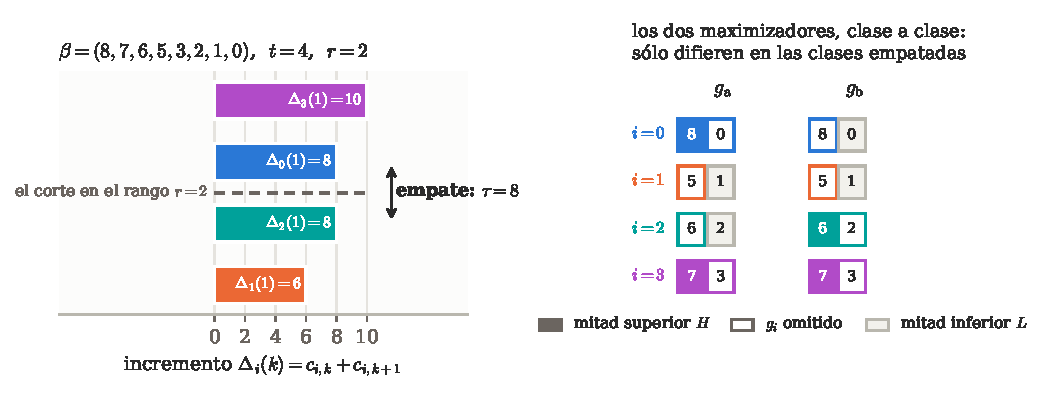
\includegraphics[width=\textwidth]{fig_increments_es.pdf}
\caption{El Teorema \ref{thm:Ggen} hecho sobre una forma, en vez de enunciado. Para
$\beta=(8,7,6,5,3,2,1,0)$ con $t=4$, $r=2$ las cuatro clases de exceso son $\{8,0\}$, $\{5,1\}$,
$\{6,2\}$, $\{7,3\}$ y los cuatro incrementos son $\Delta_3(1)=10$, $\Delta_0(1)=8$,
$\Delta_2(1)=8$, $\Delta_1(1)=6$. Un maximizador toma los $r=2$ mayores; el segundo y el tercero son
iguales, así que $\tau=\Delta_{(2)}=\Delta_{(3)}=8$ y hay exactamente dos. La pareja empatada
pertenece a las clases $0$ y $2=0+t/2$, que es \eqref{eq:congrgen} y no una casualidad: ningún valor
lo comparten incrementos de clases distintas de $i$ e $i+t/2$. A la derecha los dos maximizadores
están dibujados clase a clase en la forma de prefijo del Paso 2 --- leyendo una clase en orden
decreciente, primero los elementos de la mitad de arriba, luego el omitido $g_i$, luego los de la
mitad de abajo ---, lo que hace visible que difieren en las clases empatadas y en ninguna otra. El
color codifica la clase, no el rango. Calculada por \texttt{anc/fig\_v2.py}.}
\label{fig:increments}
\end{figure}

\begin{corollary}[un maximizador único]\label{cor:uniquegen}
Si $|G|=1$ entonces $\Phi_{t,r}\not\equiv0$.
\end{corollary}

\begin{proof}
Por \eqref{eq:topgen} la componente del numerador en grado $D_1$ es $\pm V\,P(T_g)\ne0$ para el único
$g$. Un polinomio de Laurent con una componente homogénea no nula no es nulo, así que el numerador no
es nulo y por tanto tampoco lo es $\Phi_{t,r}$.
\end{proof}

\begin{corollary}[el bloque central]\label{cor:midgen}
Escríbase $\mathcal{S}=\{s_1>\dots>s_n\}$, $n=2r+e$. Si el bloque $\{s_{r+1},\dots,s_{r+e}\}$
contiene exactamente un elemento de cada clase de exceso, entonces $\Phi_{t,r}\not\equiv0$.
\end{corollary}

\begin{proof}
$\deg(\mathcal{S}\setminus g)\le(s_1+\dots+s_r)-(s_{n-r+1}+\dots+s_n)$, porque los $r$ elementos
mayores de $\mathcal{S}\setminus g$ están dominados término a término por $s_1,\dots,s_r$ y sus $r$
menores dominan a $s_{n-r+1},\dots,s_n$. La igualdad obliga a que $\mathcal{S}\setminus g$ contenga
los dos bloques extremos, es decir $g\subseteq\{s_{r+1},\dots,s_{r+e}\}$, y $|g|=e$ fuerza la igualdad
de los dos conjuntos. Así que la cota la alcanza exactamente un término y se aplica el Corolario
\ref{cor:uniquegen}.
\end{proof}

\begin{corollary}[$t$ impar]\label{cor:oddgen}
Sea $t$ impar y $r\ge1$. Entonces $\Phi_{t,r}(\lambda;z)\equiv0$ si y sólo si alguna clase de residuos
módulo $t$ está ausente de $\beta(\lambda)$.
\end{corollary}

\begin{proof}
Si algún $n_i=0$ entonces $\mathcal T=\varnothing$ en el Lema \ref{lem:L3gen} y el numerador se anula.
Recíprocamente, si todos los $n_i\ge1$ entonces $|G|=1$ por el Teorema \ref{thm:Ggen}(c) y se aplica
el Corolario \ref{cor:uniquegen}.
\end{proof}

\begin{remark}
Para $r=1$ el Corolario \ref{cor:oddgen} es la Proposición \ref{rem:lattice}, demostrada allí viendo
que la cláusula concéntrica es vacua para $t$ impar --- un argumento interno al perfil de dos clases
que fuerza un solo par recíproco. Lo nuevo es que el enunciado sobrevive para todo $r\ge1$, y por una
ruta que no menciona el perfil en absoluto: la congruencia \eqref{eq:congrgen}. En $r=0$ es falso,
puesto que la regla de Littlewood da $s_\lambda(\zt)=0$ siempre que el $t$-núcleo es no vacío, $t$
impar incluido; y la observación de que $\prod\zt=+1$ para $t$ impar no lo entrega por sí sola,
porque el alfabeto es un subtoro de dimensión $r$ con las coordenadas restantes congeladas.
\end{remark}

% ---- v2_block3_es.tex ----
\subsection{El criterio en \texorpdfstring{$t=2$}{t=2}: rigidez y reflexión}\label{sec:rigidity}

El Corolario \ref{cor:uniquegen} resuelve toda forma con un maximizador único. Lo que sigue es la
otra mitad: cuando $|G|=2$, los dos términos de \eqref{eq:topgen} sólo pueden cancelarse si las dos
transversales son reflexión una de otra, y esa rigidez la aporta un único resultado ajeno.

\begin{theorem}[Purbhoo--van Willigenburg {\cite[Thm.~2.5]{PvW}}]\label{thm:PvW}
Para particiones con a lo sumo $n$ partes, escribiendo $\lambda^{-}:=\lambda/(\lambda_n)^{n}$,
\[
  s_\lambda(x_1,\dots,x_n)\,s_\mu(x_1,\dots,x_n)=s_\nu(x_1,\dots,x_n)\,s_\rho(x_1,\dots,x_n)
\]
si y sólo si $\lambda_n+\mu_n=\nu_n+\rho_n$ y $\{\lambda^{-},\mu^{-}\}=\{\nu^{-},\rho^{-}\}$ como
multiconjuntos.
\end{theorem}

\begin{remark}
El Teorema 3 de \cite{Rajan} da el enunciado para $n$ factores, pero bajo la hipótesis de que todos
los pesos máximos sean no nulos. El Teorema \ref{thm:PvW} no necesita tal hipótesis, y por eso es el
que usamos aquí: el caso degenerado, un factor trivial, es exactamente lo que produce el Lema
\ref{lem:dictgen} siempre que $\alpha^{*}$ o $\tilde\alpha$ es vacía. Ninguno de los dos enunciados
puede atajarse por factorización única, ya que los polinomios de Schur no son irreducibles:
$s_{(3)}(x,y)=(x+y)(x^2+y^2)$.
\end{remark}

\subsubsection*{El diccionario}

Escríbase $T=(u_1>\dots>u_{2r})$ con mitades $H=(h_1>\dots>h_r)$ y $L=(l_1>\dots>l_r)$, sea
$\delta=(r-1,r-2,\dots,0)$, de modo que $a_\delta(z)=\det(z_j^{\,r-i})$ es el determinante de
Vandermonde en la notación de la \S\ref{sec:extremal}, y póngase
\[
  \alpha=H-\delta,\qquad \tilde\alpha=\alpha-(\alpha_r)^{r},\qquad
  L^{*}=(l_1-l_r>\dots>l_1-l_1),\qquad \alpha^{*}=L^{*}-\delta .
\]

\begin{lemma}[el diccionario]\label{lem:dictgen}
$\alpha^{*}_r=0$ y
\begin{equation}\label{eq:dictgen}
  P(T)\;=\;(-1)^{\binom r2}\Bigl(\textstyle\prod_j z_j\Bigr)^{h_r-l_1}
  a_\delta(z)^2\,s_{\tilde\alpha}(z)\,s_{\alpha^{*}}(z).
\end{equation}
En particular $P$ no cambia bajo $T\mapsto T+m$ ni, por el Lema \ref{lem:reflgen}, bajo
$T\mapsto c-T$.
\end{lemma}

\begin{proof}
$a_H(z)=s_\alpha(z)a_\delta(z)$ es la fórmula bialternante. Para el segundo factor, multiplicar la
columna $j$ de $\det(z_j^{-l_i})$ por $z_j^{l_1}$ da
$(\prod_j z_j^{l_1})a_L(z^{-1})=\det(z_j^{\,l_1-l_i})$, cuyos exponentes de fila crecen con $i$;
invertir las $r$ filas cuesta $(-1)^{\binom r2}$ y produce $a_{L^{*}}(z)=s_{\alpha^{*}}(z)a_\delta(z)$.
Finalmente $s_\alpha=(\prod_j z_j)^{\alpha_r}s_{\tilde\alpha}$ y $\alpha_r=h_r$.
\end{proof}

\begin{proposition}[la órbita de $P$]\label{prop:orbitgen}
Sean $T,\widetilde T$ conjuntos de $2r$ enteros distintos con $P(T)=\pm P(\widetilde T)$. Entonces
$\widetilde T=T+m$ para algún $m\in\ZZ$, o bien $\widetilde T=c-T$ para algún $c\in\ZZ$.
\end{proposition}

\begin{proof}
Dos observaciones primero. El signo es $+$: por \eqref{eq:dictgen} los dos lados son un monomio por
$a_\delta^2$ por un producto de dos polinomios de Schur, que tiene coeficientes no negativos, así que
un signo menos es imposible. Y el monomio hay que reabsorberlo: con $d=h_r-l_1\ge1$, lo que se cumple
porque $T$ es estrictamente decreciente, $(\prod_j z_j)^{d}s_{\tilde\alpha}=s_{\tilde\alpha+(d^{r})}$,
y es ese $d$ el que hace el papel de $\lambda_n+\mu_n$ en el Teorema \ref{thm:PvW}, estando
$\alpha^{*}$ ya normalizada. Cancelando $a_\delta^2$ y aplicando el Teorema \ref{thm:PvW} con $n=r$ a
$(\lambda,\mu)=(\tilde\alpha+(d^{r}),\alpha^{*})$ y al par correspondiente $(\nu,\rho)$ de
$\widetilde T$, el criterio dice que el entero $d$ coincide y que $\{\tilde\alpha,\alpha^{*}\}$
coincide como multiconjunto. Coincidir en el mismo orden dice que $H,\widetilde H$ y $L,\widetilde L$
son trasladados, y la igualdad de los dos enteros $d$ fuerza la misma traslación en las dos mitades,
es decir $\widetilde T=T+m$. Coincidir tras intercambiar dice que $H$ es, salvo traslación, la
inversa de $\widetilde L$ y $L$ la de $\widetilde H$, es decir $\widetilde T=c-T$.
\end{proof}

\subsubsection*{Los dos maximizadores se reflejan}

De aquí al final de la subsección supóngase $|G|=2$ y escríbase
$G=\{g_{\mathrm a},g_{\mathrm b}\}$, $T_{\mathrm a}=\mathcal{S}\setminus g_{\mathrm a}$,
$T_{\mathrm b}=\mathcal{S}\setminus g_{\mathrm b}$, con mitades
$T_{\mathrm a}=H_{\mathrm a}\sqcup L_{\mathrm a}$ y $T_{\mathrm b}=H_{\mathrm b}\sqcup L_{\mathrm b}$,
y
\[
  \mathcal{K}=T_{\mathrm a}\cap T_{\mathrm b}.
\]
Por el Teorema \ref{thm:Ggen}(b) las dos transversales difieren exactamente en las clases empatadas
$i$ e $i'=i+t/2$, digamos
\begin{equation}\label{eq:swapgen}
  g_{\mathrm a}\ni p_1=c_{i,k+1},\ q_1=c_{i',k'},\qquad
  g_{\mathrm b}\ni p_2=c_{i,k},\ q_2=c_{i',k'+1},
\end{equation}
de modo que $p_1+p_2=q_1+q_2=\tau$ por \eqref{eq:incrgen}: el valor del empate es la suma de cada
pareja intercambiada.

\begin{proposition}[la traslación fuerza la reflexión]\label{prop:translgen}
Si $T_{\mathrm b}=T_{\mathrm a}+m$ con $m\ne0$, entonces $T_{\mathrm b}=\tau-T_{\mathrm a}$.
\end{proposition}

\begin{proof}
$|T_{\mathrm a}\cap(T_{\mathrm a}+m)|=|\mathcal{K}|=2r-2$. Póngase una arista $x\to x+m$ cuando $x$ y
$x+m$ estén los dos en $T_{\mathrm a}$; como $m\ne0$, cada vértice tiene a lo sumo una arista
saliente y una entrante, así que el grafo es una unión disjunta de caminos dirigidos. Tiene $2r$
vértices y, por el cardinal anterior, exactamente $2r-2$ aristas, luego exactamente dos componentes.
Así que $T_{\mathrm a}$ es unión de exactamente dos progresiones aritméticas maximales de paso $m$,
digamos $T_{\mathrm a}=\{p,p+m,\dots,p+(u-1)m\}\cup\{q,\dots,q+(v-1)m\}$ con $u+v=2r$. Entonces
$T_{\mathrm a}\setminus T_{\mathrm b}=\{p,q\}$ y $T_{\mathrm b}\setminus T_{\mathrm a}=\{p+um,q+vm\}$.
El empate dice que $x\mapsto\tau-x$ lleva la primera pareja sobre la segunda, y hay dos
emparejamientos. Si $\tau-p=p+um$ y $\tau-q=q+vm$ entonces
$\tau-T_{\mathrm a}=\{p+m,\dots,p+um\}\cup\{q+m,\dots,q+vm\}=T_{\mathrm b}$. Si $\tau-p=q+vm$ y
$\tau-q=p+um$, restando queda $um=vm$, luego $u=v$, y otra vez
$\tau-T_{\mathrm a}=T_{\mathrm b}$.
\end{proof}

\begin{proposition}[el centro es el valor del empate]\label{prop:centregen}
Si $T_{\mathrm b}=c-T_{\mathrm a}$ entonces $c=\tau$.
\end{proposition}

\begin{proof}
$x\mapsto c-x$ es una involución que lleva $T_{\mathrm a}$ a $T_{\mathrm b}$, luego $T_{\mathrm b}$ a
$T_{\mathrm a}$, luego $\mathcal{K}$ a $\mathcal{K}$; por tanto lleva
$T_{\mathrm a}\setminus\mathcal{K}$ sobre $T_{\mathrm b}\setminus\mathcal{K}$. Por \eqref{eq:swapgen}
esos dos conjuntos son $T_{\mathrm a}\setminus\mathcal{K}=\{p_2,q_2\}$ y
$T_{\mathrm b}\setminus\mathcal{K}=\{p_1,q_1\}$, ya que $T_{\mathrm a}$ omite exactamente $p_1,q_1$ y
$T_{\mathrm b}$ omite exactamente $p_2,q_2$. O bien $c-p_2=p_1$, y entonces $c-q_2=q_1$, de donde
$c=p_1+p_2=\tau$; o bien $c-p_2=q_1$ y $c-q_2=p_1$, y sumando queda
$2c=p_1+p_2+q_1+q_2=2\tau$, otra vez $c=\tau$. En el segundo caso además
$c=p_2+q_1\equiv i+i'\equiv2i+t/2$ mientras que $\tau\equiv2i$ por \eqref{eq:congrgen}, así que
$c=\tau$ forzaría $t/2\equiv0\pmod t$, imposible para $t\ge2$: el emparejamiento cruzado no ocurre.
\end{proof}

\begin{corollary}[la reflexión]\label{cor:reflectgen}
Si $\bigl[\det(x_i^{\beta_j})\bigr]_{D_1}=0$ entonces $|G|=2$ y $T_{\mathrm b}=\tau-T_{\mathrm a}$.
En consecuencia $\tau-\mathcal{K}=\mathcal{K}$ y, como $x\mapsto\tau-x$ también fija $\{p_1,p_2\}$ y
$\{q_1,q_2\}$ como conjuntos,
\begin{equation}\label{eq:Ssymgen}
  \tau-\bigl(\mathcal{K}\cup\{p_1,p_2,q_1,q_2\}\bigr)=\mathcal{K}\cup\{p_1,p_2,q_1,q_2\}.
\end{equation}
\end{corollary}

\begin{proof}
$|G|=1$ queda excluido por el Corolario \ref{cor:uniquegen}. Con $|G|=2$, \eqref{eq:topgen} y
$w(g)=\pm1$ dan $P(T_{\mathrm a})=\pm P(T_{\mathrm b})$; se aplica la Proposición
\ref{prop:orbitgen} y luego las Proposiciones \ref{prop:translgen} y \ref{prop:centregen}. La
identidad $\tau-\mathcal{K}=\mathcal{K}$ es la primera línea de la prueba de la Proposición
\ref{prop:centregen}, y $p_1+p_2=q_1+q_2=\tau$ es el empate.
\end{proof}

\begin{remark}[tres constantes fáciles de confundir]
$\tau=\Delta_{(r)}$ es el valor del empate, un dato del algoritmo voraz ajeno a toda simetría; $c$ es
un centro de reflexión, producido por la rigidez y sin nada que ver con los residuos;
$C=\min\mathcal{S}+\max\mathcal{S}$ es un estadístico del beta-conjunto, y es el que usa la condición
\textup{(ii)}. Que $c=\tau$ \textup{(}Proposición \ref{prop:centregen}\textup{)} y que $C=\tau$
\textup{(}Corolario \ref{cor:Ctaugen}\textup{)} son teoremas, no notación, y los dos necesitan la
hipótesis de anulación: escribir $C$ donde corresponde $\tau$ demuestra menos de lo que parece.
Nosotros cometimos ese desliz; de ahí los tres símbolos.
\end{remark}

\subsubsection*{El centro del beta-conjunto}

Los dos maximizadores coinciden fuera de las clases empatadas, así que su parte omitida común
\begin{equation}\label{eq:gcomgen}
  g_{\mathrm{com}}:=g_{\mathrm a}\cap g_{\mathrm b},\qquad
  \mathcal{S}=\mathcal{K}\ \sqcup\ g_{\mathrm{com}}\ \sqcup\ \{p_1,p_2,q_1,q_2\}
\end{equation}
es vacía exactamente cuando $e=2$. Por \eqref{eq:Ssymgen} el conjunto
$\mathcal{S}\setminus g_{\mathrm{com}}$ es estable bajo $x\mapsto\tau-x$, pero $g_{\mathrm{com}}$ no
tiene por qué serlo, así que $\mathcal{S}$ tampoco. Eso es más de lo que hace falta: sólo los dos
\emph{extremos} de $\mathcal{S}$ tienen que evitar $g_{\mathrm{com}}$, y lo hacen. La Figura
\ref{fig:reflection} dibuja tanto la reflexión como la forma que tiene $|G|=2$ sin ella, que es lo
que la proposición siguiente debe excluir.

\begin{figure}[!ht]
\centering
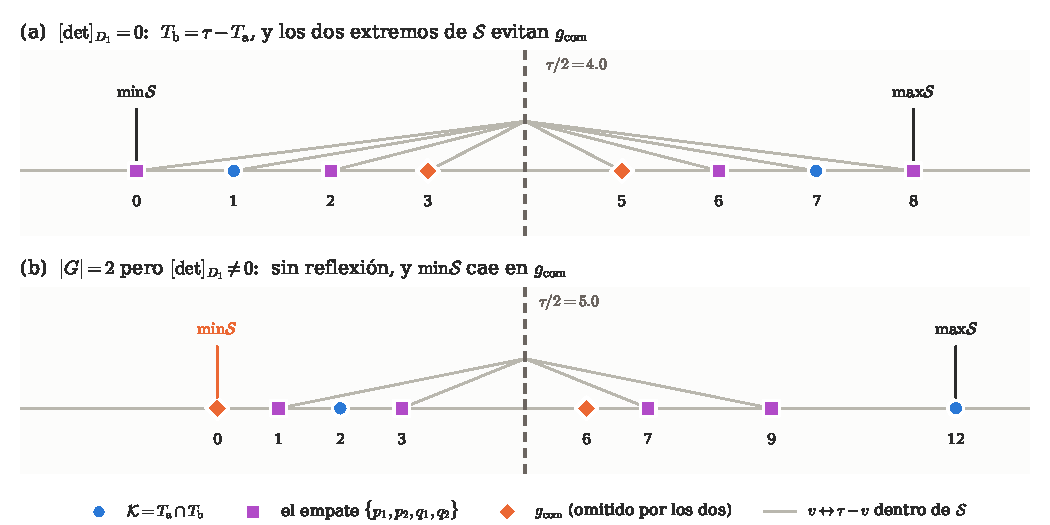
\includegraphics[width=\textwidth]{fig_reflection_es.pdf}
\caption{El Corolario \ref{cor:reflectgen} y la Proposición \ref{prop:A1gen} sobre dos formas, las
dos con $t=4$, $r=2$ y $|G|=2$. Cada panel dibuja $\mathcal{S}$ sobre una recta, coloreada según a
qué parte de \eqref{eq:gcomgen} pertenece el valor; un arco une $v$ con $\tau-v$ cuando los dos están
en $\mathcal{S}$, y la línea discontinua es el centro $\tau/2$. \emph{(a)} $\beta=(8,7,6,5,3,2,1,0)$:
$\tau=8$, $\mathcal{K}=\{1,7\}$, $g_{\mathrm{com}}=\{3,5\}$, empate $\{0,2,6,8\}$. Aquí
$T_{\mathrm b}=\tau-T_{\mathrm a}$, así que $\mathcal{S}\setminus g_{\mathrm{com}}$ es simétrico
respecto de $\tau/2$, y los dos extremos de $\mathcal{S}$ evitan $g_{\mathrm{com}}$, luego
$C=0+8=\tau$. Aquí $g_{\mathrm{com}}=\{3,5\}$ resulta ser simétrico también ---el arco que une sus
dos miembros se dibuja como cualquier otro---, que es lo que la Conjetura \ref{conj:gcom} afirma en
general y lo que la \S\ref{sec:rigidity} no demuestra: la reflexión queda establecida sobre
$\mathcal{S}\setminus g_{\mathrm{com}}$ y observada en el resto.
\emph{(b)} $\beta=(12,9,7,6,3,2,1,0)$: aquí $\tau=10$, y otra vez $|G|=2$, pero los dos maximizadores no
son reflexión uno de otro; $\min\mathcal{S}=0$ cae en $g_{\mathrm{com}}$, y $C=0+12=12\neq\tau$. El
panel (b) es la razón de que la Proposición \ref{prop:A1gen} no pueda demostrarse sólo a partir de
$|G|=2$. Calculada por \texttt{anc/fig\_v2.py}.}
\label{fig:reflection}
\end{figure}


\begin{proposition}[los extremos evitan la parte común]\label{prop:A1gen}
Supóngase $\bigl[\det(x_i^{\beta_j})\bigr]_{D_1}=0$. Entonces
$\max\mathcal{S}\notin g_{\mathrm{com}}$ y $\min\mathcal{S}\notin g_{\mathrm{com}}$.
\end{proposition}

\begin{proof}
Por el Corolario \ref{cor:reflectgen}, $T_{\mathrm b}=\tau-T_{\mathrm a}$. Como $x\mapsto\tau-x$
invierte el orden, lleva la mitad de abajo de $T_{\mathrm a}$ a la de arriba de $T_{\mathrm b}$ y al
revés:
\begin{equation}\label{eq:halvesgen}
  H_{\mathrm b}=\tau-L_{\mathrm a},\qquad L_{\mathrm b}=\tau-H_{\mathrm a}.
\end{equation}
Recuérdese del Paso 2 de la prueba del Teorema \ref{thm:Ggen} que un maximizador queda descrito por
los enteros $k_i$: dentro de la clase $i$, leída en orden decreciente, los primeros $k_i$ valores de
exceso están en la mitad de arriba, el siguiente es el omitido $g_i$, y los restantes están en la
mitad de abajo. Recuérdese también del Teorema \ref{thm:Ggen}(a) que un maximizador selecciona todo
incremento $>\tau$, que los incrementos de una clase se seleccionan en orden de prefijo, y que los
únicos incrementos iguales a $\tau$ son los dos empatados, que viven en las dos clases empatadas.

\emph{El máximo.} Póngase $m=\max\mathcal{S}$ y sea $i$ su clase, de modo que $m=c_{i,1}$ y
$n_i\ge2$; escríbase $c=c_{i,2}$. Entonces $m\in g_{\mathrm a}\cap g_{\mathrm b}$ si y sólo si
$k_i=0$ en los dos maximizadores. Supóngase que sí. Entonces la clase $i$ no está empatada: un
maximizador que toma el incremento empatado de una clase empatada tiene allí $k_i\ge1$. Luego ningún
incremento de la clase $i$ es $\ge\tau$ y, en particular,
\[
  \Delta_i(1)=m+c<\tau .
\]
Por otro lado $k_i=0$ coloca $c$ en la mitad de abajo de los dos maximizadores, así que
$c\in L_{\mathrm b}$, y \eqref{eq:halvesgen} da $\tau-c\in H_{\mathrm a}\subseteq\mathcal{S}$, de
donde $\tau-c\le\max\mathcal{S}=m$, esto es $\tau\le m+c$. Las dos desigualdades mostradas se
contradicen.

\emph{El mínimo} es la imagen especular. Póngase $m^{-}=\min\mathcal{S}$, sea $i^{-}$ su clase,
$n=n_{i^{-}}\ge2$ y $c'=c_{i^{-},n-1}$, de modo que $m^{-}=c_{i^{-},n}$. Entonces
$m^{-}\in g_{\mathrm a}\cap g_{\mathrm b}$ si y sólo si $k_{i^{-}}=n-1$ en los dos, es decir si y
sólo si los dos maximizadores seleccionan \emph{todos} los incrementos de la clase $i^{-}$; otra vez
la clase $i^{-}$ no puede estar empatada, ya que el maximizador que no toma el incremento empatado de
una clase empatada omite allí uno. Luego todo incremento de la clase $i^{-}$ supera a $\tau$, en
particular $\Delta_{i^{-}}(n-1)=m^{-}+c'>\tau$. Y $k_{i^{-}}=n-1$ coloca $c'$ en la mitad de arriba
de los dos, así que $c'\in H_{\mathrm b}$, y \eqref{eq:halvesgen} da
$\tau-c'\in L_{\mathrm a}\subseteq\mathcal{S}$, de donde $\tau-c'\ge\min\mathcal{S}=m^{-}$, esto es
$\tau\ge m^{-}+c'$. Contradicción.
\end{proof}

\begin{corollary}[el centro es el valor del empate]\label{cor:Ctaugen}
Si $\bigl[\det(x_i^{\beta_j})\bigr]_{D_1}=0$ entonces $C:=\min\mathcal{S}+\max\mathcal{S}=\tau$, y
$\mathcal{S}$ corta a todas las clases de residuos de las dos empatadas. Además $t$ es par y las dos
clases empatadas son exactamente las dos soluciones de $2\kappa\equiv C\pmod t$, ambas en
$\mathcal{E}$.
\end{corollary}

\begin{proof}
Por \eqref{eq:Ssymgen} el conjunto $\mathcal{S}\setminus g_{\mathrm{com}}$ es estable bajo
$x\mapsto\tau-x$, así que su mayor y su menor elemento suman $\tau$; por la Proposición
\ref{prop:A1gen} los dos extremos de $\mathcal{S}$ están en ese conjunto, luego \emph{son} su mayor y
su menor elemento, y $C=\tau$. El Teorema \ref{thm:Ggen}(b) da $t$ par y las dos clases empatadas
$i,i+t/2$, ambas en $\mathcal{E}$; por \eqref{eq:congrgen} $\tau\equiv2i\pmod t$, así que
$2\kappa\equiv\tau=C$ tiene exactamente las dos soluciones $\kappa=i$ y $\kappa=i+t/2$.
\end{proof}

\begin{corollary}[una condición necesaria, para todo $t$ par y todo $r$]\label{cor:necgen}
Sean $t\ge2$ y $r\ge1$, y supongamos $\Phi_{t,r}(\lambda;z)\equiv0$ con todo $n_i\ge1$. Entonces $t$
es par, $|G|=2$, $\min\mathcal{S}+\max\mathcal{S}=\tau$, y $\mathcal{S}\setminus g_{\mathrm{com}}$ es
simétrico respecto de $\tau/2$.
\end{corollary}

\begin{proof}
$\Phi_{t,r}$ y el numerador difieren en un factor no nulo, así que el numerador se anula
idénticamente y en particular $\bigl[\det(x_i^{\beta_j})\bigr]_{D_1}=0$. Se aplican los Corolarios
\ref{cor:reflectgen} y \ref{cor:Ctaugen} y \eqref{eq:Ssymgen}.
\end{proof}

\noindent Esto es lo que sobrevive de las \S\S\ref{sec:extremal}--\ref{sec:rigidity} fuera de $t=2$.
Lo que \emph{no} da es el paso que cierra $t=2$: allí $e=2$ obliga a $g_{\mathrm{com}}=\varnothing$, y
la simetría de $\mathcal{S}\setminus g_{\mathrm{com}}$ pasa a ser la simetría del propio $\beta$. Para
$t\ge4$ la parte común $g_{\mathrm{com}}$ puede no ser vacía, y el argumento de arriba no dice nada
de ella: la reflexión queda establecida sólo sobre $\mathcal{S}\setminus g_{\mathrm{com}}$, de modo
que restringe a $\beta$ sin llegar a determinarlo. Que $g_{\mathrm{com}}$ sea simétrico también es lo
que muestran las medidas y lo que enuncia la Conjetura \ref{conj:gcom}; aquí no se demuestra.

\subsubsection*{La condición es suficiente, para todo \texorpdfstring{$t$}{t} y todo
\texorpdfstring{$r$}{r}}

Una condición necesaria invita a su recíproco, y la mitad se consigue de una pieza. La reflexión que
el Corolario \ref{cor:necgen} extrae del estrato superior resulta ser, cuando vale sobre todo
$\mathcal{S}$ y no sólo sobre una parte, una simetría de \emph{cada} término de la suma de Laplace y
no únicamente de los dos maximizadores; y una involución sin puntos fijos cancela lo que empareja.
Escribimos
\[
C:=\min\mathcal{S}+\max\mathcal{S},\qquad\text{y escribimos } x\mapsto C-x
\text{ para la reflexión que centra.}
\]

\begin{theorem}[la dirección suficiente, para todo $t$ y todo $r$]\label{thm:suff}
Sean $t\ge2$, $r\ge1$, $N=t+2r$, y supongamos ocupada toda clase de residuos. Supongamos que
\begin{equation}\label{eq:suffcond}
C-\mathcal{S}=\mathcal{S}
\qquad\text{y}\qquad
\Delta_i(k)=C\ \text{para algún } i\in\mathcal{E},\ k .
\end{equation}
Entonces $\Phi_{t,r}(\lambda;z)\equiv0$.
\end{theorem}

Las dos cláusulas hacen dos trabajos distintos, y conviene decir cuál es cuál antes de la prueba: la
primera hace que la reflexión \emph{actúe} sobre las transversales, y la segunda hace que esa acción
sea \emph{libre}. La Figura \ref{fig:pairing} es el mecanismo entero sobre una sola forma, con otra al
lado que cumple la primera cláusula y no la segunda.

\begin{figure}[!ht]
\centering
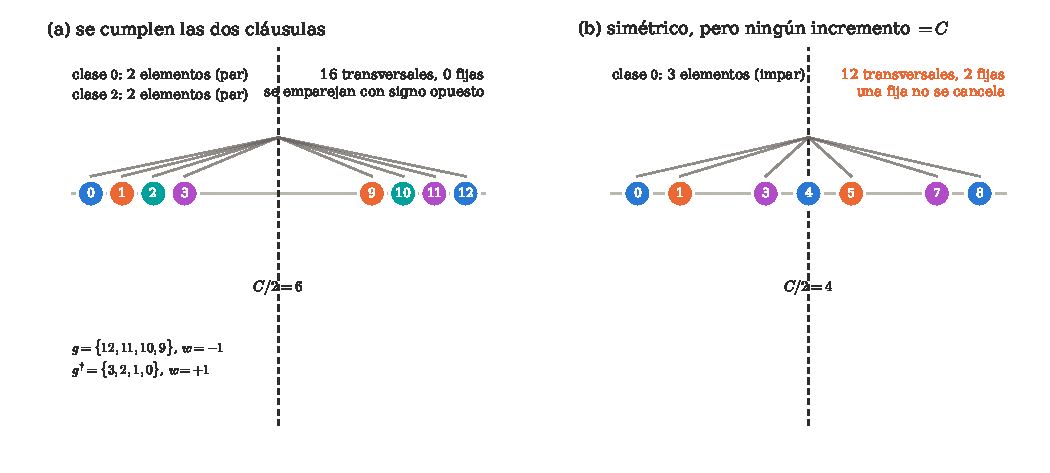
\includegraphics[width=\textwidth]{fig_pairing_es.pdf}
\caption{Por qué se cancela la suma, y para qué está la segunda cláusula. Cada panel dibuja
$\mathcal{S}$ sobre una recta, coloreado por clase de residuo, con un arco que une $v$ con $C-v$ y el
eje de puntos en $C/2$. \emph{(a)} $\beta=(12,11,10,9,3,2,1,0)$ con $t=4$, $r=2$: las dos clases que
la reflexión fija tienen tamaño \emph{par}, así que ninguna contiene a $C/2$; las $16$ transversales
se emparejan sin ningún punto fijo, y cada pareja lleva signos opuestos, de modo que cada término de
\eqref{eq:laplacegen} lo cancela otro. Una de esas parejas está impresa con sus dos signos,
calculados y no afirmados. \emph{(b)} una forma con $C-\mathcal{S}=\mathcal{S}$ pero sin ningún
incremento igual a $C$, encontrada buscándola y no elegida: allí la clase fija tiene tamaño
\emph{impar}, luego contiene a $C/2$, y dos transversales son su propio reflejo. Un término
emparejado consigo mismo no puede cancelarse, y la suma sobrevive. Eso es todo lo que compra la
segunda cláusula. Calculada por \texttt{anc/fig\_involution2.py}.}
\label{fig:pairing}
\end{figure}

\begin{lemma}[la transversal reflejada]\label{lem:reflact}
Supongamos $C-\mathcal{S}=\mathcal{S}$. Entonces $x\mapsto C-x$ lleva la clase $i$ sobre la clase
$i^{*}:=C-i \bmod t$, y o las dos están en $\mathcal{E}$ o ninguna; de modo que
\[
g^{\dagger}:=\bigl(C-(g\cap\mathcal{S})\bigr)\cup\bigl(g\setminus\mathcal{S}\bigr)
\]
es de nuevo una transversal, $g\mapsto g^{\dagger}$ es una involución sobre ellas, y
$T_{g^{\dagger}}=C-T_g$.
\end{lemma}

\begin{proof}
Todo elemento de la clase $i$ es $\equiv i$, así que $x\mapsto C-x$ lo manda dentro de la clase
$i^{*}$; como $C-\mathcal{S}=\mathcal{S}$ y la aplicación es inyectiva, lleva la clase $i$
\emph{sobre} la clase $i^{*}$ siempre que $i\in\mathcal{E}$, lo que obliga a $i^{*}\in\mathcal{E}$ y a
$n_i=n_{i^{*}}$. Las clases unitarias no se tocan: su único elemento está congelado en toda
transversal. Por último $T_{g^{\dagger}}=\mathcal{S}\setminus g^{\dagger}=C-(\mathcal{S}\setminus
g)=C-T_g$.
\end{proof}

\begin{lemma}[el menor reflejado]\label{lem:Arefl}
$A(C-T)=A(T)$ para todo $2r$-conjunto $T$ y todo $C$.
\end{lemma}

\begin{proof}
% Sin "=" en esta frase: TeX parte la formula en linea despues de la relacion y deja el signo
% colgando fuera del margen, y forzarla con \mbox la echa entera fuera.  Se dice con palabras.
Sacar $x_i^{C}$ de cada una de las $2r$ filas multiplica el determinante por el factor
$\prod_j z_j^{C}z_j^{-C}$, que vale $1$, y deja la matriz de $T$ con $x_i$ sustituido por
$x_i^{-1}$, que es la
matriz de $T$ con las dos filas de cada par recíproco intercambiadas: un signo $(-1)^{r}$.
Y listar $C-T$ en orden decreciente invierte el orden de las columnas, lo que aporta
$(-1)^{\binom{2r}{2}}$, es decir $(-1)^{r}$, porque $2r-1$ es impar. Los dos se cancelan.
\end{proof}

\noindent Los dos movimientos de esa prueba no son nuestros, y merece la pena decir de quién son,
porque son el instrumento adecuado y los elegimos por eso. Escalar cada fila por una potencia para
sustituir $x_i$ por $\bar x_i$, y luego invertir un bloque de columnas para recoger
$(-1)^{n(n-1)/2}$, es la maniobra que Ayyer y Behrend emplean sobre el bialternante de una forma
autocomplementaria \cite[\S3]{AB19}; ellos mismos describen sus pruebas como apoyadas sólo en las
expresiones determinantales ``y la aplicación de operaciones estándar con determinantes'', y ésta es
una de esas operaciones. Albion hace la misma inversión del lado de las raíces de la unidad
\cite{Alb23,Alb25}, y a nivel de caracteres el mismo hecho es la invariancia de $sp_\lambda$ bajo
$x_i\mapsto\bar x_i$, recogida en \cite{AB19} y puesta a trabajar en \cite{AF20}.

Conviene explicar por qué es útil aquí, porque es lo que hace corta toda la sección. A un menor
reflejado se le puede atacar desarrollándolo, y entonces habría que seguir término a término las
clases unitarias y las reflejadas --- que es como lo intentamos primero, y no se acaba nunca. La
maniobra de Ayyer y Behrend, en cambio, liquida la reflexión en \emph{dos} cálculos de signo que no
miran las entradas en ningún momento, y es robusta justo en el sentido que necesitamos: no usa en
ningún paso que se esté reflejando el alfabeto entero, así que sobrevive al aplicarse a una
\emph{parte} del conjunto beta, con el resto quieto. Esa robustez es la razón de que el Lema
\ref{lem:Arefl} ocupe cuatro líneas y no una sección, y pertenece a la herramienta y no a nosotros.
Es además un indicio menor a favor de la tesis de la \S\ref{sec:background}: las dos líneas entre las
que se sitúa este artículo comparten más maquinaria de lo que sus enunciados dejan ver.

El enunciado que sigue es el corazón combinatorio del argumento, y sólo necesita la primera cláusula
de \eqref{eq:suffcond}. Reflejar un conjunto beta \emph{entero} es clásico --- es la identidad de
complementación \eqref{eq:compl}, y los pasos determinantales que hay detrás son los estándar que
acabamos de citar. Lo que aquí se pide es la reflexión de la parte de exceso \emph{sola}, con las
clases unitarias quietas e intercaladas entre los valores reflejados; las dos involuciones que eso
produce, una de $\beta$ y otra de $\ZZ/t$, son de las que acaba dependiendo el signo.

\begin{lemma}[la fórmula del signo de la reflexión parcial]\label{lem:signformula}
Supongamos $C-\mathcal{S}=\mathcal{S}$, y pongamos
\[
\nu=\#\{x\in\mathcal{S}:2x=C\},\qquad \eta=\#\{i\in\mathcal{E}:2i\equiv C \bmod t\}.
\]
Entonces, para toda transversal $g$,
\begin{equation}\label{eq:wrefl}
\frac{w(g^{\dagger})}{w(g)}\;=\;(-1)^{\,e-\frac{\nu+\eta}{2}} .
\end{equation}
En particular el cociente no depende de $g$, ni de $r$, ni de $N$.
\end{lemma}

\begin{corollary}\label{cor:whenminus}
Bajo $C-\mathcal{S}=\mathcal{S}$, el cociente \eqref{eq:wrefl} vale $-1$ si y sólo si $\eta=2$.
\end{corollary}

\begin{proof}
Una involución tiene tantos puntos fijos como elementos su conjunto, módulo dos, así que
$\nu\equiv|\mathcal{S}|$ y $\eta\equiv e$; y $|\mathcal{S}|=2r+e$ por \eqref{eq:excessgen}, luego
también $\nu\equiv e$. Si $e$ es impar, entonces $\nu=\eta=1$ y el exponente es $e-1$, par. Si $e$ es
par, entonces $\nu=0$ y $\eta$ vale $0$ ó $2$, lo que da el exponente $e$ ó $e-1$; el primero es par y
el segundo impar.
\end{proof}

\noindent Esa independencia es la parte que parece improbable y es justo la que importa: las clases
unitarias están colocadas en posiciones arbitrarias entre los valores reflejados, y mover una
transversal las hace cruzarse unas con otras --- pero cada cruce que aportan a la suma de columnas lo
deshace el cruce que aportan a la palabra de residuos, así que no dejan rastro en el cociente.

\begin{lemma}[el signo reflejado]\label{lem:signrefl}
Supongamos \eqref{eq:suffcond}. Entonces $\eta=2$, el número $e$ es par, $\nu=0$, y
$w(g^{\dagger})=-w(g)$ para toda transversal $g$.
\end{lemma}

\begin{proof}[Prueba del Lema \ref{lem:signformula}]
Sea $\mathcal{R}$ la aplicación $x\mapsto C-x$ sobre $\mathcal{S}$ y la identidad sobre
$\beta\setminus\mathcal{S}$, y sea $\mathcal{R}_t$ la aplicación $i\mapsto i^{*}$ sobre $\mathcal{E}$
y la identidad fuera; ambas son involuciones, de $\beta$ y de $\ZZ/t$ respectivamente, con $\nu$ y
$\eta$ puntos fijos, así que $\sgn(\mathcal{R})=(-1)^{(|\mathcal{S}|-\nu)/2}$ y
$\sgn(\mathcal{R}_t)=(-1)^{(e-\eta)/2}$. Ordenemos las columnas de una transversal $g$ por residuo y
las restantes por $\beta$ decreciente; el signo de la permutación de $\{1,\dots,N\}$ que resulta es
$w(g)$ salvo un factor que depende sólo de $t$. Aplicar $\mathcal{R}$ a esa notación de una línea
aporta $\sgn(\mathcal{R})$; restablecer el orden por residuo del primer bloque aporta
$\sgn(\mathcal{R}_t)$; y $\mathcal{R}$ invierte $T_g$ por completo, de modo que restablecer su orden
decreciente aporta $(-1)^{\binom{2r}{2}}$. Multiplicando los tres sale \eqref{eq:wrefl}, donde ningún
término se refiere a $g$.
\end{proof}

\begin{proof}[Prueba del Lema \ref{lem:signrefl}]
Contar puntos fijos de una involución da $|\mathcal{S}|\equiv\nu$ y $e\equiv\eta \pmod 2$, y
$|\mathcal{S}|=2r+e$ por \eqref{eq:excessgen}, luego $e\equiv\nu$. Ahora bien, la segunda cláusula de
\eqref{eq:suffcond} dice que dos elementos \emph{adyacentes} de alguna clase $i_0$ suman $C$; la
reflexión los intercambia, así que $i_0=i_0^{*}$, y escribiendo la clase en orden decreciente el
intercambio manda su $k$-ésima entrada a la $(n_{i_0}+1-k)$-ésima, de donde $n_{i_0}=2k$ es par. La
reflexión $x\mapsto C-x$ tiene a lo sumo un punto fijo, que es $C/2$; como esta clase es estable bajo
ella y tiene cardinal par, sus elementos se emparejan y no contiene ninguno, luego $C/2\notin$ clase
$i_0$.

Antes de hablar de una segunda solución hay que saber que la hay, y ahí es donde la paridad de $t$ se
decide en vez de suponerse. Supongamos $t$ impar. Entonces $2$ es invertible módulo $t$, así que
$i\mapsto i^{*}$ tiene a $i_0$ como su \emph{único} residuo fijo; las demás clases de $\mathcal{E}$ se
emparejan, luego $e$ es impar, y $|\mathcal{S}|=2r+e$ también. Una involución sobre un conjunto de
tamaño impar tiene un punto fijo, así que $\nu=1$ y $C/2\in\mathcal{S}$; su residuo $\kappa$ cumple
$2\kappa\equiv C$, luego $\kappa=i_0$, lo que sitúa a $C/2$ en la clase $i_0$ --- que acabamos de ver
que no lo contiene. Así que $t$ es par, y $2i\equiv C$ tiene exactamente las dos soluciones $i_0$ e
$i_1=i_0+t/2$.

Si $\nu=1$, entonces $C/2\in\mathcal{S}$ y su residuo es $i_0$ o $i_1$; no es $i_0$, luego
$i_1\in\mathcal{E}$. Si $\nu=0$, entonces $e$ es par, y $\mathcal{E}=\{i_0\}\sqcup\{\text{pares}\}$
haría $e$ impar salvo que $i_1\in\mathcal{E}$. En cualquiera de los dos casos $\eta=2$, luego $e$ es
par y $\nu=0$, y el Corolario \ref{cor:whenminus} da el signo de inmediato. Leyendo \eqref{eq:wrefl}
directamente, el exponente es $e-\tfrac{0+2}2=e-1\equiv1 \pmod 2$.
\end{proof}

\begin{corollary}[la hipótesis, leída sobre los residuos]\label{cor:suffgeom}
Supongamos $C-\mathcal{S}=\mathcal{S}$. Entonces algún $\Delta_i(k)=C$ si y sólo si $t$ es par y
\emph{las dos} soluciones de $2i\equiv C \pmod t$ son clases de exceso. Dicho de otro modo,
\eqref{eq:suffcond} afirma: la parte de exceso del conjunto beta es simétrica respecto de $C/2$, y las
dos clases de residuos que la reflexión fija son ambas de exceso.
\end{corollary}

\begin{proof}
Una dirección es el primer párrafo de la prueba del Lema \ref{lem:signrefl}. Para la otra, si las dos
clases fijas están en $\mathcal{E}$ entonces $\eta=2$, luego $e$ es par por $e\equiv\eta$, luego
$|\mathcal{S}|=2r+e$ es par y $\nu=0$: ningún elemento de $\mathcal{S}$ queda fijo. Una clase fija es
entonces estable por la reflexión y sin puntos fijos, luego de tamaño par $2k$, y sus entradas
$k$-ésima y $(k+1)$-ésima se intercambian, así que $\Delta_i(k)=C$.
\end{proof}

\noindent Leída así, la hipótesis tiene la misma forma que la conclusión del Corolario
\ref{cor:Ctaugen}, y eso es lo que hace que las dos mitades de la sección se miren la una a la otra:
allí las dos clases empatadas \emph{resultan} ser las dos soluciones de $2\kappa\equiv C$; aquí
\emph{pedimos} que sean de exceso.

\begin{proof}[Prueba del Teorema \ref{thm:suff}]
Por el Lema \ref{lem:reflact}, $g\mapsto g^{\dagger}$ es una involución sobre las transversales con
$T_{g^{\dagger}}=C-T_g$. No tiene puntos fijos: una transversal fija necesitaría $C-g_i=g_i$, es
decir $g_i=C/2$, en toda clase con $i=i^{*}$, y la clase $i_0$ de la prueba anterior es una de ésas y
no contiene a $C/2$. Por los Lemas \ref{lem:Arefl} y \ref{lem:signrefl},
\[
w(g)A(T_g)+w(g^{\dagger})A(T_{g^{\dagger}})=w(g)A(T_g)-w(g)A(C-T_g)=0 ,
\]
así que la suma de \eqref{eq:laplacegen} se cancela por parejas y el numerador se anula
idénticamente.
\end{proof}

\begin{remark}[qué es esto, y qué no es]\label{rem:suffscope}
Conviene separar tres cosas. Primera: en $t=2$ la hipótesis \eqref{eq:suffcond} \emph{es} la rama
{\rm(b)}; allí $e=2$ obliga a $\mathcal{S}=\beta$, con lo que $C-\mathcal{S}=\mathcal{S}$ es la
autocomplementariedad, y la cláusula del incremento es la paridad de la anchura --- los dos enunciados
coinciden en todas las formas de los rangos de la \S\ref{sec:verif}. Así que el Teorema
\ref{thm:suff} contiene esa mitad del Teorema \ref{conj:crit}, y la prueba otra vez por un mecanismo
distinto. Segunda: para $t\ge4$ \emph{no} es complementación; allí $\mathcal{S}\subsetneq\beta$,
$\lambda$ no es autocomplementaria, y \eqref{eq:compl} no dice nada. Tercera: la involución es global
--- empareja \emph{todos} los términos de \eqref{eq:laplacegen} y no sólo los dos maximizadores ---, y
por eso sobrevive donde el argumento extremal sólo produce una condición necesaria.
\end{remark}

\begin{conjecture}[el criterio, en general]\label{conj:general}
Recíprocamente, si $\Phi_{t,r}(\lambda;z)\equiv0$ y toda clase de residuos está ocupada, entonces vale
\eqref{eq:suffcond}. Equivalentemente, para todo $t$ y todo $r$,
\[
\Phi_{t,r}(\lambda;z)\equiv0
\iff
\text{alguna clase es vacía, o } C-\mathcal{S}=\mathcal{S}\text{ y algún }\Delta_i(k)=C .
\]
\end{conjecture}

\noindent Bajo la hipótesis de anulación, casi todo lo que pide \eqref{eq:suffcond} ya se sabe, y
decir qué parte convierte la conjetura en una sola frase sobre un solo conjunto. El Corolario
\ref{cor:Ctaugen} da $C=\tau$, luego los incrementos empatados valen $C$ y la segunda cláusula se
cumple; y \eqref{eq:Ssymgen} da $C-(\mathcal{S}\setminus g_{\mathrm{com}})=\mathcal{S}\setminus
g_{\mathrm{com}}$. Como $\mathcal{S}=(\mathcal{S}\setminus g_{\mathrm{com}})\sqcup g_{\mathrm{com}}$,
lo único que queda es esto:

\begin{conjecture}[la parte común es simétrica]\label{conj:gcom}
Bajo ocupación, si $\Phi_{t,r}(\lambda;z)\equiv0$ entonces $C-g_{\mathrm{com}}=g_{\mathrm{com}}$.
\end{conjecture}

\noindent Las Conjeturas \ref{conj:general} y \ref{conj:gcom} son el mismo enunciado, y la segunda es
la forma útil: nombra los $e-2$ elementos a los que el argumento tiene que llegar, y ningunos más.
Dice también, de una vez, por qué $t=2$ cierra y $t\ge4$ no. En $t=2$ un empate es entre las clases
$i$ e $i+1$, de modo que las dos son de exceso y $e=2$ ---no porque allí $e=2$ valga siempre, pues
\eqref{eq:excessgen} permite $e=1$ y es frecuente, sino porque $|G|=2$ lo obliga, y
$g_{\mathrm{com}}$ sólo está definido cuando $|G|=2$---. Por tanto $g_{\mathrm{com}}=\varnothing$ y
no queda nada que pueda ser simétrico. El teorema no es allí más
fácil; sencillamente no hay parte común.

Los enunciamos como conjeturas y no como teoremas porque sólo está probada la dirección de arriba. La
evidencia está en la \S\ref{sec:verif}: sobre $190\,443$ formas en veinticuatro configuraciones, con
$t\le12$ y $r\le4$, el criterio no tiene ningún falso positivo ni ningún falso negativo; $43\,010$
de ellas se rehacen con una evaluación que no comparte código con esta sección, y un barrido más de
$12\,937$ formas, con $131$ ceros, se rehace en Sage, que no comparte con ninguna de las dos ni
código ni biblioteca; en los rangos donde ya
decide un teorema, coincide con el Teorema \ref{thm:main} en $r=1$ y con el Teorema \ref{conj:crit} en
$t=2$ sin una sola discrepancia, sobre $9913$ y $29\,508$ formas; y un señuelo que lee la condición
sobre $\beta$ en vez de sobre $\mathcal{S}$ --- esto es, la autocomplementariedad de la forma en lugar
de la de su parte de exceso --- falla en todas las configuraciones de ambos barridos. Lo que falta es
una implicación: el Corolario \ref{cor:necgen} da la reflexión sobre $\mathcal{S}\setminus
g_{\mathrm{com}}$, y el estrato superior no puede dar más --- hay formas que comparten $\tau$,
$\mathcal{S}\setminus g_{\mathrm{com}}$ y las clases empatadas, y de las cuales unas se anulan y otras
no, así que la ecuación que falta no es un refinamiento de la \S\ref{sec:rigidity} sino un enunciado
sobre un estrato inferior.

\begin{remark}[por qué no el argumento obvio]
Lo primero que se intenta es un intercambio dentro de un \emph{solo} maximizador: si
$\max\mathcal{S}$ está omitido, re-elegir su clase y esperar que suba el grado. No puede funcionar.
Un maximizador puede omitir $\max\mathcal{S}$ --- justo cuando $\max\mathcal{S}$ es uno de los valores
empatados $p_1,p_2$, de modo que un maximizador lo omite y el otro lo conserva ---, así que ningún
argumento que lea una transversal cada vez concluye. La Proposición \ref{prop:A1gen} es un enunciado
sobre el \emph{par}, y por eso la prueba corre sobre \eqref{eq:halvesgen} y sobre nada más. El Cuadro
\ref{tab:extremal} recoge tanto los pasos de esa prueba como lo que le pasa a su conclusión cuando se
quita la hipótesis.
\end{remark}

\begin{table}[!ht]
\centering\small
\caption{La maquinaria de las \S\S\ref{sec:extremal}--\ref{sec:rigidity}, medida. La población es
toda forma con $|G|=2$ sobre $(t,r)\in\{4,6,8,10\}\times\{2,3\}$ dentro de las anchuras barridas. La
última fila es la que importa para la Proposición \ref{prop:A1gen}: al quitar la hipótesis
$[\det]_{D_1}=0$ la conclusión falla, así que no viene de balde.}
\label{tab:extremal}
\begin{tabular}{@{}llrl@{}}
\toprule
enunciado & población & resultado & guion \\
\midrule
\rowcolor{hband} parametrización voraz $=$ fuerza bruta & $4049$ formas & \textcolor{hproved}{$0$ fallos} & \texttt{a1\_proof} \\
$A$ es la mitad de arriba de $T_g$ (Paso 2) & la misma & \textcolor{hproved}{$0$ fallos} & \texttt{a1\_proof} \\
\rowcolor{hband} $T_{\mathrm b}=\tau-T_{\mathrm a}$ & $2522$ formas & \textcolor{hproved}{$0$ fallos} & \texttt{a1\_proof} \\
$v\in L_{\mathrm b}\Rightarrow\tau-v\in H_{\mathrm a}$ & $3034$ valores & \textcolor{hproved}{$0$ fallos} & \texttt{a1\_proof} \\
\rowcolor{hband} los extremos evitan $g_{\mathrm{com}}$ & $2522$ formas & \textcolor{hproved}{$0$ fallos} & \texttt{a1\_proof} \\
las identidades mostradas de estas subsecciones & $11$ identidades & \textcolor{hproved}{$0$ fallos} & \texttt{v2\_formulas} \\
\midrule
\rowcolor{hband} lo mismo, quitando $[\det]_{D_1}=0$ & $24718$ formas & \textcolor{hverif}{$414$ fallos} & \texttt{a1\_proof} \\
\bottomrule
\end{tabular}
\end{table}

\begin{remark}
El Corolario \ref{cor:reflectgen} hace trabajo de verdad en la Proposición \ref{prop:A1gen}, y
$|G|=2$ por sí solo no basta. Para $t=4$, $r=2$ y $\beta=(200,199,198,197,194,193,191,4)$ las clases
de exceso son $\{200,4\}$, $\{197,193\}$, $\{198,194\}$, $\{199,191\}$ y los incrementos son
$392,390,390,204$, así que $\tau=390$, el empate es entre las clases $1$ y $3$, y $|G|=2$. Pero
$\Delta_0(1)=204<\tau$, así que $k_0=0$ en los dos maximizadores y $\max\mathcal{S}=200$ lo omiten los
dos: la conclusión de la Proposición \ref{prop:A1gen} falla. Aquí $T_{\mathrm a}=(198,197,191,4)$ y
$T_{\mathrm b}=(199,198,193,4)$ no son reflexión una de otra --- $h_r-l_1$ vale $6$ para la primera y
$5$ para la segunda --- y en consecuencia la componente de grado $D_1$ no se anula.
\end{remark}

\begin{figure}[!ht]
\centering
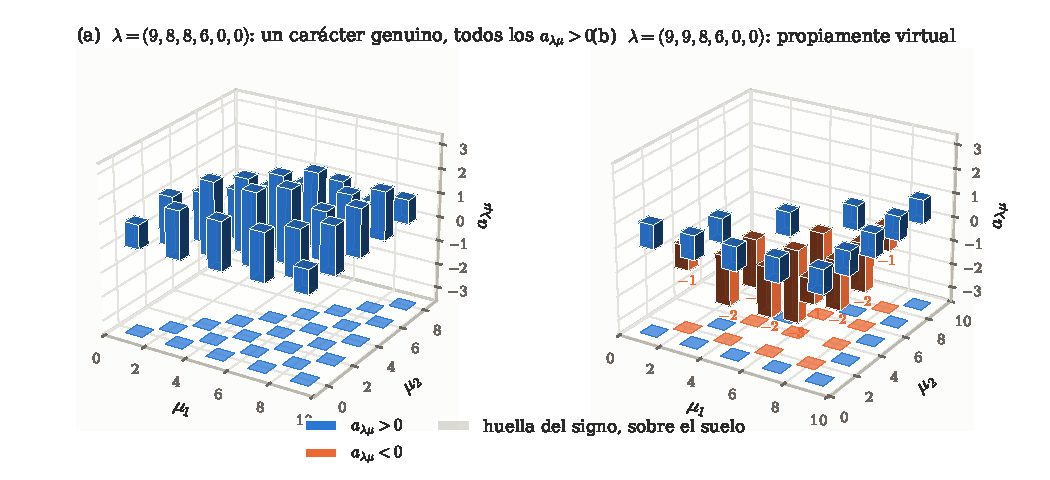
\includegraphics[width=\textwidth]{fig_virtual_es.pdf}
\caption{Por qué un solo par recíproco no es lo típico, en $r=2$: la expansión
$\Psi_r(\lambda)=\sum_\mu a_{\lambda\mu}\,sp_\mu(z)$ sobre los pesos dominantes de $Sp(4)$. Las dos
formas difieren en una sola casilla. Para $\lambda=(9,8,8,6,0,0)$ todo $a_{\lambda\mu}$ es positivo:
el objeto es un carácter genuino, como lo es para \emph{toda} $\lambda$ cuando $r=1$, donde el
Teorema \ref{thm:main} lo escribe como producto de tres caracteres de $\mathfrak{sl}_2$. Para
$\lambda=(9,9,8,6,0,0)$ la expansión tiene $12$ coeficientes positivos y $10$ negativos, siendo el más
negativo $-3$: es genuinamente virtual, que es el fenómeno que recoge la Observación
\ref{rem:rankone} y la razón de que un cálculo en el extremo deje de ser un test exacto pasado un
par. Los dos paneles comparten la escala vertical, y los cuadrados planos del suelo repiten el signo
de cada coeficiente, porque un coeficiente $-1$ es invisible al lado de uno $+3$. Calculada por
\texttt{anc/fig\_v2.py}.}
\label{fig:virtual}
\end{figure}

\subsubsection*{El criterio en \texorpdfstring{$t=2$}{t=2}}

\begin{proof}[Demostración del Teorema \ref{conj:crit}]
La implicación de (a) o (b) a $\Psi_r(\lambda)=0$ es el Teorema \ref{thm:zeros}. Para el recíproco,
supóngase $\Psi_r(\lambda)=\Phi_{2,r}(\lambda;z)\equiv0$ y que ninguna clase de residuos módulo $2$
falta en $\beta(\lambda)$, ya que en otro caso se cumple la rama (a) y no hay nada que probar.
Entonces el numerador se anula idénticamente, así que en particular su componente de grado $D_1$ se
anula y $|G|=2$ por el Corolario \ref{cor:uniquegen}.

Por el Teorema \ref{thm:Ggen}(b) hay un empate en el rango $r$ entre las clases $i$ e $i+t/2=i+1$; en
$t=2$ ésas son las dos clases, y ambas están en $\mathcal{E}$, luego $e=2$. (Con $e=1$ todos los
incrementos viven en una sola clase y son distintos dos a dos por el Paso 4, así que no hay empate
posible.) Como $e=2$, ninguna clase es unitaria y $\mathcal{S}=\{\beta_1,\dots,\beta_N\}$ es el
beta-conjunto entero.

Por el Corolario \ref{cor:Ctaugen}, $C=\min\mathcal{S}+\max\mathcal{S}=\beta_N+\beta_1=\tau$ y, como
cambian las dos clases, $g_{\mathrm{com}}=\varnothing$ en \eqref{eq:gcomgen}, de modo que
\eqref{eq:Ssymgen} se lee $\tau-\mathcal{S}=\mathcal{S}$: el beta-conjunto es simétrico respecto de
$C$, es decir
\[
  \beta_j+\beta_{N+1-j}=C\qquad\text{para todo }j .
\]
Sustituyendo $\beta_j=\lambda_j+N-j$ esto se convierte en $\lambda_j+\lambda_{N+1-j}=C-N+1=:w$ para
todo $j$, que es la auto-complementariedad de anchura $w=\lambda_1+\lambda_N$. Finalmente, el
Corolario \ref{cor:Ctaugen} dice que las dos soluciones de $2\kappa\equiv C\pmod2$ son las dos
clases, lo que ocurre exactamente cuando $C$ es par; y $C=w+N-1$ con $N=2r+2$ par, así que $C$ par es
exactamente $w$ impar. Luego $\lambda$ es auto-complementaria de anchura impar: la rama (b).
\end{proof}

\begin{remark}
En $t=2$ la congruencia \eqref{eq:congrgen} es vacua --- todo incremento es par --- y $|G|\le2$ vale
por la razón más débil de que sólo existen dos clases. Lo que \emph{no} es vacuo en $t=2$ es que
$\tau$ sea par, y se usa dos veces: prohíbe el emparejamiento cruzado en la Proposición
\ref{prop:centregen}, y \emph{es} la paridad que se convierte en la rama (b).
\end{remark}

\begin{remark}[\emph{genuino} no quiere decir \emph{irreducible}]
En la Observación \ref{rem:rankone}, \emph{$\pm$ un carácter genuino} significa una combinación
\emph{no negativa} de irreducibles, no uno solo. No es uno solo: ya
$s_{(2)}(1,-1,z,z^{-1})=z^{2}+2+z^{-2}=sp_{(2)}+sp_{(0)}$. En $t=2$, $r=1$ el Teorema
\ref{thm:main} da un producto de tres caracteres de $\mathfrak{sl}_2$, y un producto de caracteres es
un carácter --- ésa es toda la afirmación. A partir de $r=2$ aparecen coeficientes negativos y no
existe ninguna representación, que es lo que quiere decir \emph{genuinamente virtual}; el Cuadro
\ref{tab:virtual} cuenta las dos cosas y la Figura \ref{fig:virtual} dibuja una de cada.
\end{remark}

\begin{table}[!ht]
\centering\small
\caption{Genuino frente a genuinamente virtual, sobre todas las $\lambda$ con $\lambda_1$ hasta la
cota indicada. La expansión es $\Psi_r(\lambda)=\sum_\mu a_{\lambda\mu}\,sp_\mu(z)$; \emph{un signo}
quiere decir que todos los $a_{\lambda\mu}$ tienen el mismo signo, de modo que $\pm\Psi_r$ es un
carácter, y \emph{mezclado} quiere decir que es genuinamente virtual. En $r=1$ la columna de mezclados
está vacía, como fuerza el Teorema \ref{thm:main}; no lo está para ningún $r\ge2$ al que lleguemos.
Calculada por \texttt{anc/fig\_v2.py}.}
\label{tab:virtual}
\begin{tabular}{@{}lrrrr@{}}
\toprule
 & \multicolumn{1}{c}{formas} & \multicolumn{1}{c}{$\Psi_r=0$} & \multicolumn{1}{c}{un signo}
 & \multicolumn{1}{c}{mezclado} \\
\midrule
\rowcolor{hband} $r=1$, $\lambda_1\le14$ & $3060$ & $352$ & $2708$ & \textcolor{hproved}{$\mathbf{0}$} \\
$r=2$, $\lambda_1\le8$  & $3003$ & $78$ & $2531$ & \textcolor{hverif}{$\mathbf{394}$} \\
$r=3$, $\lambda_1\le5$  & $1287$ & $27$ & $1008$ & \textcolor{hverif}{$\mathbf{252}$} \\
$r=4$, $\lambda_1\le2$  & $66$   & $2$  & $58$   & \textcolor{hverif}{$\mathbf{6}$} \\
\bottomrule
\end{tabular}
\end{table}

\begin{remark}[dónde vive el alfabeto]
Para $r=1$ el alfabeto $(1,-1,z,\bar z)$ de \eqref{eq:psir} es literalmente la lista de valores
propios de una matriz de la componente no identidad $O(4)^{-}$, tabulada como tal por Hanany y
Kalveks \cite[Tabla 7]{HK16}, que además registran la caída de rango
$[\mathrm{vec}]_{O(2n)^{-}}\cong[\mathrm{vec}]_{O(2)^{-}}\oplus[\mathrm{fund}]_{C_{n-1}}$ para la
representación \emph{vectorial}. Así que $\Psi_r$ es un carácter de $GL(2r+2)$ evaluado en esa
componente, y el plegado $D_{r+1}\to C_r$ es la razón de que aparezca un grupo simpléctico; no lo
usamos más que para situar el objeto, ya que para una $\lambda$ cualquiera la restricción es una
combinación con coeficientes enteros de caracteres simplécticos, y no uno solo.
\end{remark}

\section{Verificación}\label{sec:verif}

Todos los enunciados anteriores se comprobaron numéricamente, con tres implementaciones por rutas de
código distintas: una en aritmética de Laurent exacta, otra una evaluación del bialternante escrita
desde cero a partir de los enunciados, y una tercera en Sage, que no comparte con las otras dos ni
una línea de código ni una biblioteca. Los rangos y recuentos se recogen aquí una sola vez.

% longtable y no tabular: con un tabular esta tabla es una caja indivisible, y LaTeX la empuja
% entera a la pagina siguiente dejando la de la cabecera de seccion casi vacia.  longtable parte por
% paginas y repite la cabecera, que es lo que una tabla de cuarenta filas necesita.
% \raggedright en las dos primeras: justificadas, una columna estrecha estira los espacios y deja
% "t <= 7, |lambda| <=" con huecos enormes.  La tercera va \raggedleft porque son cifras.
\begingroup\footnotesize\setlength{\tabcolsep}{4.0pt}
% Anchuras algo menores que en la edicion inglesa: el castellano es mas largo por palabra y con las
% de alla la tabla se salia 4 pt.  Se miden en el PDF, no en el log.
\begin{longtable}{@{}>{\raggedright\arraybackslash}p{0.352\linewidth}%
                  >{\raggedright\arraybackslash}p{0.222\linewidth}%
                  >{\raggedleft\arraybackslash}p{0.272\linewidth}@{\hspace{4pt}}l@{}}
\toprule
enunciado & rango & resultado & estado\\
\midrule
\endfirsthead
\multicolumn{4}{@{}l}{\footnotesize\itshape Verificación, continuación}\\[1pt]
\toprule
enunciado & rango & resultado & estado\\
\midrule
\endhead
\midrule
\multicolumn{4}{r@{}}{\footnotesize\itshape sigue en la página siguiente}\\
\endfoot
\bottomrule
\endlastfoot
Teor. \ref{thm:main}, signo incluido & $t\le7$, $|\lambda|\le14,\dots,10$ &
$959$ exactos, $476$ ceros, $0$ fallos & \stproved\\
\quad lo mismo, una implementación escrita desde el enunciado & $t\le6$, $|\lambda|\le12,\dots,9$ &
$749$ formas, $0$ fallos; el señuelo del signo falla $35/133$ & \stproved\\
Lema \ref{lem:L1} & $t\le6$ & $454$ menores no nulos & \stproved\\
Lema \ref{lem:L4} & $t\le7$ & $724/724$ & \stproved\\
Proposición \ref{prop:quotient} & $t\le7$, $|\lambda|\le19$ & $2970/2970$ & \stproved\\
Prop. \ref{rem:lattice} (lugar concéntrico) & $t\le9$, $|\lambda|\le16$ & $1331/1331$;
$0$ con $t$ impar, $43$ con par & \stproved\\
Prop. \ref{rem:sign} (forma corta del signo) & $t\le8$, $|\lambda|\le14$ & $1496/1496$;
pasos de la prueba, $0$ fallos & \stproved\\
\quad la ley de desplazamiento \eqref{eq:shift} y su signo & $t\le7$, $|\lambda|\le12$ &
$826$ formas, $0$ fallos & \stproved\\
Prop. \ref{prop:minimal} (el multiconjunto separa) & $d_i\le60$; $t\le5$, $|\lambda|\le16$ &
$75640$ invariantes, $0$ colisiones & \stproved\\
\quad lo mismo, en los dos sentidos, desde el enunciado & $t\le5$, $|\lambda|\le14,\dots,11$ &
$676$ formas, $0$ colisiones; señuelo $104$ & \stproved\\
Prop. \ref{prop:fibrelattice} (el retículo) & $t\le5$, $|\lambda|\le14,12,10,10$ &
$84$, $35$, $20$, $14$ fibras, en ambos sentidos & \stproved\\
Cor. \ref{cor:fibregf} (función generatriz) & mismo rango &
$153/153$; denominador erróneo $101$ & \stproved\\
Observación \ref{rem:signsees} (el signo ve los $m_i$) & $t\le4$ &
$107/107$, $43/62$, $26/36$ & \stverif\\
Lema \ref{lem:single} & $t\le7$, $|\lambda|\le16$ & $2113/2113$ & \stproved\\
Teor. \ref{thm:extra} & $t\le12$, $\lambda_1\le33$ & $119+21$, ninguna más & \stproved\\
\quad el signo es $+1$, \eqref{eq:extrainv} & $t\le14$ par; núcleos $t\le10$ &
$28$ extra $+$ $219$ núcleos, todos $+1$ & \stproved\\
Proposición \ref{prop:rect} & $t=2$, $r\le4$, $c\le60$ & $240/240$ & \stproved\\
Cor. \ref{cor:enum} contra enumeración directa & $t\le5$ & $14/14$; cajas $16/16$ &
\stproved\\
Prop. \ref{rem:involution} (las rachas alternan) & $t=2$, $|\lambda|\le14$, $\le4$ filas &
$4823$ menores; $217$ pares, $0$ fallos & \stproved\\
(D3), (D4) de la \S\ref{sec:sharp} & $t\le6$, $|\lambda|\le10$ &
$600$ / $383$ / $200$ de $600$ & \stverif\\
\midrule
\rowcolor{hband} Teor. \ref{conj:crit}, el criterio, todo $r$ & --- & prueba, \S\ref{sec:rigidity} & \stproved\\
\rowcolor{hband} \quad lo mismo, leído sobre $O(N)$, Cor.~\ref{cor:dettwist} & --- &
reformulación, \S\ref{sec:conv} & \stproved\\
\rowcolor{hband} \quad Teor. \ref{thm:PvW}, el input externo & --- & \cite{PvW} & \stext\\
\rowcolor{hband} \quad Teorema \ref{thm:Ggen}, $|G|\le2$ & $t\le10$, $r\le3$ & voraz contra fuerza bruta, $0/4049$ & \stproved\\
\rowcolor{hband} \quad Prop.~\ref{prop:A1gen}, los extremos & $t\le10$, $r\le3$ & $2522$ formas, $0$ fallos & \stproved\\
\rowcolor{hband} \quad \quad la hipótesis hace falta & mismo & $414$ formas fallan sin ella & \stproved\\
\rowcolor{hband} \quad las identidades mostradas, \S\S\ref{sec:extremal}--\ref{sec:rigidity} & $t=2$, $r\le3$ & $11$ identidades, $0$ fallos & \stverif\\
\rowcolor{hband} Lema \ref{lem:step}, movimiento de columna, toda clase & $t\le6$, $r\le3$ &
$285\,600/285\,600$; señuelo de un término $149\,652$ & \stproved\\
\rowcolor{hband} Teor. \ref{thm:suff}, la dirección suficiente & $t\le8$, $r\le4$ &
$438$ formas, $0$ fallos; \eqref{eq:wrefl} $438/438$ & \stproved\\
\rowcolor{hband} Conj. \ref{conj:general}, ambas direcciones & $t\le12$, $r\le4$ &
$190\,443$ formas, $24$ configuraciones, $0$ fallos & \stverif\\
\rowcolor{hband} \quad lo mismo, evaluación independiente & $t\le8$, $r\le4$ &
$43\,010$ formas, $409$ ceros, $0$ fallos & \stverif\\
\rowcolor{hband} \quad lo mismo otra vez, en Sage & $t\le8$, $r\le3$ &
$12\,937$ formas, $131$ ceros, $0$ fallos & \stverif\\
\rowcolor{hband} \quad contra los Teoremas \ref{thm:main} y \ref{conj:crit} & $r=1$; $t=2$ &
$9913$ y $29\,508$ formas, $0$ discrepancias & \stproved\\
\rowcolor{hband} \quad el señuelo que lee $\beta$ en vez de $\mathcal{S}$ & mismo &
falla en $24$ de $24$ y en $14$ de $14$ & \stproved\\
\midrule
\rowcolor{hband} Teor. \ref{conj:crit}, ambas direcciones, comprobación directa & $r\le3$, $|\lambda|\le28,26,22$ &
$9961$ formas, $318$ ceros, $0$ fallos & \stproved\\
\rowcolor{hband} \quad rama (a), Teor.~\ref{thm:zeros} & $r\le3$, $|\lambda|\le15$ &
$16/16$ & \stproved\\
\rowcolor{hband} \quad rama (b), Teor.~\ref{thm:zeros} & $r\le3$ & $24/24$ & \stproved\\
\rowcolor{hband} \quad control de anchura par para (b) & $r\le3$ & $56/56$ no nulos & \stproved\\
\rowcolor{hband} \quad recíproco en $r=1$, Teor.~\ref{thm:r1} & $\beta_1\le25$ &
$14950$ conjuntos beta, $0$ fallos & \stproved\\
\rowcolor{hband} \quad recíproco, $\ell(\lambda)\le N/2$, Teor.~\ref{thm:stable} & $r\le3$ &
$372/372$ testigos & \stproved\\
\rowcolor{hband} \quad el testigo aislante, Prop.~\ref{conj:iso} & $r=2$, $|\lambda|\le14$ &
$227$ testigos, $11$ de residuo & \stproved\\
\rowcolor{hband} \quad lo mismo en $r=3$ & $r=3$, $|\lambda|\le13$ &
$149$ testigos, $0$ de residuo & \stproved\\
\midrule
Identidad \eqref{eq:compl} & $r\le2$ & $474/474$ & \stproved\\
Identidad \eqref{eq:docagne}, y $\deg_{c_\ast}S_n=n-1$ & $b\le31$ & $496/496$; $39/39$ &
\stproved\\
Lema \ref{lem:AtoSp}, la reducción de la \S\ref{sec:unstable} & $r\le3$, $|\nu|\le8$ &
identidad $0$ fallos; plegados $0$ fallos & \stproved\\
\quad la reducción, llevada a cabo & $r\le2$ & $236$ etiquetas, $0$ sin resolver & \stproved\\
\eqref{eq:Cmu} contra el objeto exacto & $r\le2$, ambos rangos & $184$ formas, $0$ fallos &
\stverif\\
\end{longtable}
\endgroup

\noindent El bloque sombreado es el Teorema \ref{thm:zeros} leído de arriba abajo: las dos ramas
suficientes están demostradas para todo $r$, el recíproco está demostrado para un par y, para todo
$r$, dentro del rango de Littlewood; y la línea que solía quedar ---el recíproco para $r\ge2$ fuera
de ese rango y más allá de la franja $|\lambda|\le2r+2$ que resuelve el Lema \ref{lem:nonstd}---
es el Teorema \ref{conj:crit}, demostrado en la \S\ref{sec:rigidity} por un argumento que no entra
en el rango de Littlewood. Por eso el bloque lleva ya \stproved\ en todas sus filas, con una en
\stext\ para el apoyo ajeno del que depende. La fila que registra lo que hace y lo que no hace el
certificado que propusimos se queda, y lleva \stproved\ porque la Proposición \ref{conj:iso} es un
contraejemplo y los contraejemplos son demostraciones; lo que acota ahora es una vía, no el
enunciado. Las filas por debajo del bloque son las identidades y la reducción sobre
las que se apoya la sección. En la columna, \stproved\ significa que aquí se da una demostración o se
cita, y \stverif\ que el enunciado se comprueba de forma exhaustiva sobre el rango indicado y no se
demuestra.

\noindent La fila de (D3), (D4) es la que más importa del primer grupo: la identidad se cumple en los
$600$ casos para \eqref{eq:object} y falla en $217$ y $400$ de ellos para los dos alfabetos
deformados, de modo que el contraste es capaz de fallar. En el segundo grupo, el control de anchura
par cumple el mismo papel para el Teorema \ref{thm:zeros}: $56$ formas autocomplementarias de anchura
par, ninguna de las cuales se anula, así que la hipótesis de paridad trabaja en lugar de decorar. Una
auditoría aparte reconstruye todo el segundo grupo desde las definiciones en una sola pasada, con
independencia de los guiones que los produjeron: $3414$ comprobaciones, $0$ fallos. Una segunda toma
las \emph{fórmulas mostradas} en vez de los recuentos ---el Teorema \ref{thm:LR}, la lectura por
intervalos \eqref{eq:intervals}, los Lemas \ref{lem:L2} y \ref{lem:L5}, la partición
\eqref{eq:threestep}, la complementación \eqref{eq:compl}, d'Ocagne \eqref{eq:docagne} y la
advertencia escalar \eqref{eq:scalar}--- y evalúa ambos miembros en puntos numéricos desde las
definiciones, sin usar ni las formas cerradas de este artículo ni los guiones que sostienen la
tabla: $3297$ evaluaciones sobre nueve fórmulas mostradas, $0$ fallos. Los guiones son
material auxiliar de este artículo, y también lo es la salida guardada de cada uno, de modo que todo
recuento de la tabla anterior puede localizarse en una ejecución archivada en lugar de aceptarse por
confianza.

%======================================================================
\section{Problemas abiertos}\label{sec:open}

La Figura \ref{fig:map} sitúa lo que sigue frente a lo que el artículo demuestra y lo que toma
prestado; los problemas de abajo son las cajas que deja abiertas.

\begin{figure}[!ht]
\centering
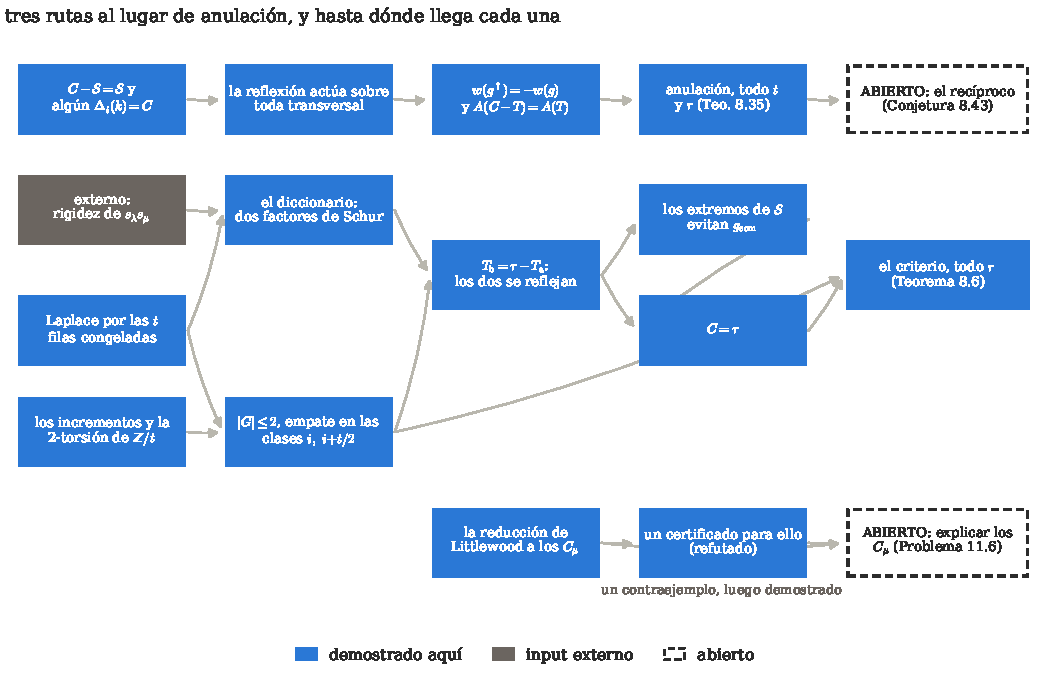
\includegraphics[width=\textwidth]{fig_map_es.pdf}
\caption{Sobre qué se apoya el criterio de la \S\ref{sec:zeros} y qué queda. Las cajas son
enunciados y las flechas dependencias; el color es la columna de estado de la \S\ref{sec:verif} ---
relleno lo demostrado aquí, gris el único apoyo ajeno, discontinuo lo abierto. La rama de arriba es
el argumento extremal de las \S\S\ref{sec:extremal} y \ref{sec:rigidity}; la de abajo es la
reducción de Littlewood, cuyo certificado refuta la Proposición \ref{conj:iso} ---un contraejemplo,
o sea una demostración---, de modo que la rama de abajo ya no toca el criterio sino la cuestión
aparte de explicar los $C_\mu$, que es el Problema \ref{prob:instrument}. Los enunciados van por
nombre y no por número, para que la figura no pueda desfasarse cuando la numeración lo haga.
Calculada por \texttt{anc/fig\_proof.py}.}
\label{fig:map}
\end{figure}

\begin{problem}[los otros tipos clásicos]\label{prob:types}
Todo lo anterior es de tipo $A$. ¿Qué hacen $sp_\lambda(\zt,z,\zb)$, $so_\lambda(\zt,z,\zb)$ y
$o_\lambda(\zt,z,\zb)$? Las factorizaciones de raíces de la unidad se llevaron del tipo $A$ a los
tipos $B$, $C$, $D$ con un argumento uniforme en \cite{AK22} y a los caracteres universales en
\cite{Alb23}; las filas congeladas del bialternante son las mismas en todos los tipos, de modo que el
Lema \ref{lem:L1} y el recuento de exceso dos deberían sobrevivir palabra por palabra, mientras que
el colapso, los Lemas \ref{lem:L4} y \ref{lem:L5}, habría que rehacerlo una vez por tipo. El alfabeto
\eqref{eq:object} es ya un elemento del toro de $O(t+2)$, de modo que los otros tipos no son la misma
función en un punto nuevo sino objetos nuevos, y elegir los correctos es cuestión de criterio dentro
de un programa que no hemos construido nosotros. Sí hemos medido, y lo damos como medición y nada
más. Desarrollando los caracteres universales de Koike--Terada en la base de Schur y evaluando
término a término con el Teorema \ref{thm:main}, sobre $|\lambda|\le12$ para $t\le3$ y
$|\lambda|\le10$ para $t=4,5$, la fracción de formas con $\ell(\lambda)\ge2$ en las que el valor se
anula es netamente mayor para $o_\lambda$ en la componente no identidad que en la identidad ---el
$83.8\%$ con $t=2$ frente al $41.8\%$ con $t=3$, y el $58.8\%$ con $t=4$ frente al $42.1\%$ con
$t=5$---, con $sp_\lambda$ en medio y el caso de Schur el más bajo. El efecto es real y sigue a la
componente, que es lo que cabría esperar de una cancelación entre asociados; pero es cuantitativo y
no le hemos encontrado ley que cubra la tabla entera. Un primer intento de ley, que $o_\lambda$ se
anule para todo
$\ell(\lambda)\ge2$ cuando $t$ es par, es falso: se leyó de una muestra y el barrido sistemático lo
refuta.

La columna $t=2$ de esa comparación es el único caso que sí tiene ley, y es el Lema
\ref{lem:AtoSp}: allí el alfabeto es \eqref{eq:psir} con $r=1$, de modo que $o_\nu$ es igual a
$sp_\nu(z)$, un carácter simpléctico de \emph{rango uno}. Ése se anula idénticamente para
$\ell(\nu)=2$ --- las $36$ formas del rango, sin excepción --- y se pliega para $\ell(\nu)>2$, que es
la razón de que la cifra de $t=2$ sea la que se sale. Lo que queda sin ley es $t$ impar, donde el
alfabeto no tiene la forma \eqref{eq:psir} y el lema no se aplica.

La columna de $sp_\lambda$ en $t=2$, en cambio, sí tiene respuesta, y explica la asimetría de la
tabla en lugar de añadirle una fila. Adjuntar esas mismas dos letras a un carácter universal
\emph{simpléctico} no lo colapsa. Sobre $|\nu|\le8$,
\begin{equation}\label{eq:spbranch}
sp_\nu(W,1,-1)\;=\;\sum_{\gamma\subseteq\nu}c_{\nu/\gamma}\;sp_\gamma(W),
\end{equation}
donde el coeficiente depende de $\nu$ y $\gamma$ solo a través de la forma sesgada $\nu/\gamma$
---$247$ coeficientes sobre $74$ formas sesgadas distintas, sin un solo choque--- y toma únicamente
los valores $0$ y $\pm1$, anulándose siempre que $|\nu/\gamma|$ es impar. Esa es la forma que produce
una regla de ramificación para funciones simplécticas universales, y tales reglas existen
\cite{JJLW24}. Leído contra ella, el Lema \ref{lem:AtoSp} dice que para $o_\nu$ los coeficientes
correspondientes se concentran en $\gamma=\nu$: las dos letras colapsan el carácter ortogonal a un
único carácter simpléctico, y dejan el simpléctico repartido por todo el intervalo bajo $\nu$. La
asimetría de la medición es eso, y no un artefacto de los rangos. Lo que no hemos hecho es
identificar $c_{\nu/\gamma}$, que \eqref{eq:spbranch} convierte en una pregunta sobre caracteres
simplécticos universales sesgados en $(1,-1)$ y en nada más.

La tercera columna se resiste a la misma vía, y por una razón estructural y no accidental. Lo que
resuelve las otras dos es que adjuntar una letra es el mapa de anillos $p_k\mapsto p_k+c^k$, de modo
que $\iota_{1}$ y $\iota_{-1}$ actúan sobre $\Lambda$ y componen. La identidad que traería $so$ al
cuadro, $so_\nu(X)=o_\nu(X,\bar X,1,0,\dots)$ de \cite[(2.13)]{AK25}, relaciona ambos sobre un
alfabeto \emph{duplicado}, y una duplicación no es una adjunción: los $\iota$ no llegan. Así que la
columna $so$ no es una laguna de esfuerzo sino de mecanismo, y la dejamos enunciada como tal.
\end{problem}

\begin{problem}[una Verschiebung que vea un par recíproco]\label{prob:versch}
El operador $\varphi_t$ no tiene nada que decir sobre una letra fuera de una $\zeta$-órbita, que es
la razón estructural de que el Teorema \ref{thm:main} no sea corolario de nada de esa línea, y la
razón de que nuestra demostración descienda al alternante. ¿Existe un operador sobre caracteres
universales, o una factorización de $\varphi_t$ a través de un álgebra mayor, que actúe sobre
alfabetos de la forma (unión de $\zeta$-órbitas) $\cup$ (pares recíprocos)? Por la \S\ref{sec:sharp},
un operador así decidiría (D1) y (D2) de una vez. La discusión de allí sugiere una forma
cuantitativa.

Lo que vuelve bien planteada la pregunta, y no vaga, es que cada mitad tiene ya un formalismo, y no
son el mismo. Las $\zeta$-órbitas son territorio de $\varphi_t$, en la formulación de Albion
\cite{Alb23}. Los alfabetos cerrados por inversión son territorio de las funciones simplécticas y
ortogonales universales, que admiten realizaciones por operadores de vértice de las que se siguen sus
reglas de ramificación \cite{JJLW24}. Nuestro alfabeto es uno de cada, y el Lema \ref{lem:AtoSp} es
el único sitio donde ambos se encuentran: allí la $\zeta$-órbita es $\{1,-1\}$, lo bastante pequeña
como para que adjuntarla sea un par de mapas de letra y no un operador. No conocemos nada que actúe
sobre las dos mitades a la vez, y la pregunta es si los dos formalismos componen.
\end{problem}

\begin{proposition}[el rango es el invariante equivocado]\label{conj:rank}
Sea $A=\zt\cup B$ con $B$ cerrado bajo inversión y disjunto de $\zt$, y sea $\rho(B)$ el rango del
subgrupo de $\CC^{\times}$ generado por $B$. Entonces $\rho(B)=1$ no implica que $s_\lambda(A)$ sea
un producto de caracteres. En $t=2$ y $B=\{z,z^{-1},z^{2},z^{-2}\}$, que tiene $\rho(B)=1$, el valor
en $\lambda=(2)$ tiene una raíz fuera de la circunferencia unidad, y por tanto no admite tal
factorización; lo mismo ocurre con $B=\{z,z^{-1},z^{3},z^{-3}\}$.
\end{proposition}

\begin{proof}
Un producto de caracteres $\chi_k(z)=(z^{k+1}-z^{-k-1})/(z-z^{-1})$ tiene todas sus raíces en la
circunferencia unidad, así que basta exhibir una raíz fuera de ella. Para
$B=\{z,z^{-1},z^{2},z^{-2}\}$ y $\lambda=(2)$ el valor es
$z^{-4}+z^{-3}+z^{-2}+z^{-1}+3+z+z^{2}+z^{3}+z^{4}$. El polinomio de Laurent es invariante bajo
$z\mapsto z^{-1}$, de modo que escribiendo $x=z+z^{-1}$ y usando $z^{k}+z^{-k}\in\ZZ[x]$ queda
\[
x^{4}+x^{3}-3x^{2}-2x+3\;=\;(x-1)\bigl(x^{3}+2x^{2}-x-3\bigr).
\]
La cúbica tiene discriminante
$18\cdot2\cdot(-1)(-3)-4\cdot2^{3}(-3)+2^{2}(-1)^{2}-4(-1)^{3}-27\cdot(-3)^{2}=-31<0$, luego dos de
sus raíces no son reales. Si $|z|=1$, entonces $x=z+z^{-1}=2\cos\theta$ es real; así que para una
raíz no real $x_0$, ninguna de las dos raíces de $z^{2}-x_0z+1=0$ está en la circunferencia unidad, y
las dos son raíces del valor. Luego la factorización es imposible, y el enunciado es exacto y no
numérico.

Sobre $|\lambda|\le8$ el mismo fenómeno ocurre en $17$ de las $62$ formas no nulas, y con
$B=\{z,z^{-1},z^{3},z^{-3}\}$ en $18$; en el mismo rango, $B=\{z,z^{-1}\}$ tiene todas sus raíces en
la circunferencia sin excepción, como exige el Teorema \ref{thm:main}.
\end{proof}

Lo que el rango no ve es cuántas direcciones libres tiene $B$. Un solo par recíproco es una
dirección; $\{z,z^{-1},z^{2},z^{-2}\}$ genera un grupo de rango uno y son dos, y las dos se ven entre
sí. Así que el invariante sobre el que conjeturar no es $\rho(B)$ sino el número de letras
independientes, y con esa lectura el enunciado pasa a ser el que la \S\ref{sec:sharp} ya hace por
otros medios:

\begin{conjecture}[una sola dirección libre]\label{conj:rank2}
Sea $B$ cerrado bajo inversión y disjunto de $\zt$, como en la Proposición \ref{conj:rank}. Entonces
$s_\lambda(\zt\cup B)$ es cero o un producto de caracteres, para toda $\lambda$, si y solo si $B$ es
un único par recíproco. (La alternativa no es decoración: por el Corolario \ref{cor:zero} el valor sí
se anula para alguna $\lambda$ ya con un par, y $0$ no es un producto de caracteres.)
\end{conjecture}

La evidencia a su favor es el Teorema \ref{thm:main} en un sentido y (D1)--(D4) junto con la
Proposición \ref{conj:rank} en el otro: agrandar $B$ destruye el producto, suba o no suba el rango la
ampliación. No tenemos demostración ni mecanismo propuesto, y es precisamente el enunciado que un
argumento del estilo de $\varphi_t$ debería producir.

Esa hipótesis es bajo la que se enuncia la conjetura, y es también la que una forma general tendría
que soltar. El cierre por inversión de $B$ es suficiente
en la evidencia anterior, pero no es necesario para que haya producto. Escribamos $w=-iy$. El segundo
bloque del alfabeto $\{1,-1,y,-y^{-1}\}$ no es cerrado por inversión y, sin embargo,
\begin{equation}\label{eq:scalar}
s_\lambda\big(1,-1,y,-y^{-1}\big)\;=\;i^{\,|\lambda|}\,s_\lambda\big(-i,\,i,\,w,\,w^{-1}\big),
\end{equation}
y el alfabeto de la derecha sí lo es. La hipótesis que llevaría una forma proyectivamente invariante
no es, por tanto, el cierre por inversión de $B$, sino que $A$ sea un múltiplo
escalar de un conjunto cerrado por inversión. Una clase lateral $\zeta\zt$ es ella misma cerrada por
inversión exactamente cuando $\zeta^{2}=\pm1$, que es donde (D3) rompe y donde no.

\begin{problem}[el instrumento para el segundo par]\label{prob:instrument}
La Sección \ref{sec:zeros} reduce la anulación en $r\ge2$ a un enunciado sobre los coeficientes
$C_\mu$ de \eqref{eq:Cmu}, que son sumas con signo de coeficientes de Littlewood. Ese enunciado ya
no es lo que falta: el Teorema \ref{conj:crit} resuelve la anulación, por el argumento extremal de
la \S\ref{sec:rigidity}, que no se cruza con ningún $C_\mu$. Lo que la reducción pide ahora no es
una demostración sino una \emph{explicación} ---por qué se cancelan esas sumas con signo, en los
propios términos de Littlewood--- y sigue sin haber certificado, pues el que propusimos falla por la
Proposición \ref{conj:iso}. Un problema que era un hueco pasa a ser una pregunta por una segunda
demostración, que es mejor problema y más pequeño. El Lema \ref{lem:AtoSp} resuelve la otra mitad de la reducción --- qué
son los valores $o_\nu(A)$ --- y la resuelve simplécticamente: las dos lecturas del alfabeto
concuerdan porque son la misma lectura, pues el álgebra órbita de $D_{r+1}$ es $C_r$ y no la
subálgebra fija $B_r$. Lo que no toca son los coeficientes. Kumari y Stokke \cite{KS26} han dado
reglas de Murnaghan--Nakayama para funciones de Schur simplécticas, ortogonales y ortosimplécticas;
por el Lema \ref{lem:AtoSp} la pertinente aquí es la simpléctica \cite[Teorema 3.4]{KS26}, y no la
ortogonal par \cite[Teorema 3.10]{KS26}. ¿Calcula su recursión los
$C_\mu$? Su regla arrastra un tercer sumando más allá de añadir y quitar tiras de borde, y es el que
ellas mismas señalan como complicado; el \cite[Corolario 3.5]{KS26} muestra que desaparece en cuanto
$\mu_n+1\ge r$, de modo que es un fenómeno de formas poco profundas. Una forma anterior de este
problema preguntaba si ese sumando es el que da cuenta del fallo de la regla de Littlewood fuera de su
rango; el Lema \ref{lem:AtoSp} responde que no, pues el fallo lo llevan las reglas de modificación
simplécticas, que actúan sobre las etiquetas y no dentro de la recursión. Lo que queda son los
coeficientes, y lo que no hemos intentado es si esa recursión los calcula.

Hay un segundo instrumento, y es el que probaríamos primero. Las reglas de ramificación de Frohmader
\cite{Frohmader} calculan $\mathrm{mult}(\pi^{\nu}_{O_n},\pi^{\lambda}_{GL_n})$ como
$\sum_{\mu}c^{\lambda}_{\mu\nu}(O_n)$ sobre las particiones $\mu$ de filas pares, sin restricción de
rango estable y sin regla de modificación. Nuestros $C_\mu$ de \eqref{eq:Cmu} son sumas con signo de
exactamente las multiplicidades que esas reglas calculan, ensambladas por la involución asociada
$\nu\mapsto\nu^{*}$. Así que la pregunta se vuelve concreta: ¿es $C_\mu(\lambda)=0$, en las dos
ramas, una identidad entre coeficientes de Littlewood--Richardson generalizados que las condiciones
de bandera hagan visible? Ésa es una pregunta sobre tablas, que es la forma en la que nos gustaría
verla contestada.
\end{problem}

\begin{problem}[el lugar adicional, en general]\label{prob:extralocus}
¿Tiene el Teorema \ref{thm:extra} análogo para $sp$, $so$ y $o$? Más en general, ¿para qué
especializaciones de las variables libres adquiere el criterio \eqref{eq:AK53} soluciones
adicionales, y puede leerse siempre el lugar adicional en el núcleo de la especialización actuando
sobre el espacio generado por los caracteres universales, como sugiere la Observación
\ref{rem:why}? Si cada tipo adquiere una familia indexada por un elemento de orden dos del retículo
de residuos, el principio es real.

La pregunta necesita fijar la parte libre, y por una razón computada: la familia extra es un
fenómeno del alfabeto \emph{mínimo}. Añádase un segundo par recíproco y desaparece ---sobre
$t=3,4,5,6$ y $|\lambda|\le14$ el lugar pasa a ser exactamente los $t$-núcleos, para el tipo $s$
tanto como para $sp$ y $o$, mientras que con un solo par el tipo $s$ tiene los dos extras del Teorema
\ref{thm:extra} en $t=4$ y uno en $t=6$. (El segundo par se prueba en $z_2=z_1^{2}$, una
especialización, que solo puede crear coincidencias y no eliminarlas, de modo que un recuento de cero
ahí es un recuento de cero.) El análogo para otro tipo hay que buscarlo, por tanto, en la parte libre
mínima \emph{de ese tipo}, una letra de cada clase; comparar tipos con partes libres de tamaños
distintos mide la parte libre, que es lo que hizo nuestro primer intento.

El núcleo es lo que hay que mirar, pero su \emph{presencia} no decide el lugar; lo decide su
tamaño. Dos partes libres del mismo tamaño pueden colapsar ambas la independencia y comportarse de
manera muy distinta. En el lugar recíproco $s_\mu(z,\zb)=\chi_{\mu_1-\mu_2}(z)$ conserva una
graduación, y el lugar extra es la única familia del Teorema \ref{thm:extra}. Sustitúyase el par
por la $\zeta_2$-órbita $(z,-z)$, donde $s_\mu(z,-z)=z^{|\mu|}s_\mu(1,-1)$ conserva sólo $|\mu|$ y
un signo, y sobre $\ell(\lambda)\le2$ el criterio adquiere $28$ soluciones más en $t=2$ y $186$ en
$t=8$, en ninguna familia que sepamos nombrar. El control es el par libre $(z,w)$, que no tiene
núcleo y devuelve los $t$-núcleos y nada más para todo $t\le8$ ---que es \eqref{eq:AK53} misma, de
modo que el control es su teorema y no una medición nuestra. Así que el par recíproco es la
especialización colapsante de núcleo \emph{mínimo}, y
eso, y no la mera existencia de un núcleo, es lo que hace que su lugar extra sea una sola familia.
\end{problem}

\begin{problem}[las fibras, refinadas por el signo]\label{prob:fibres}
El Corolario \ref{cor:fibregf} describe la fibra de la terna de intervalos, y solo eso. El
invariante es $I_t=(d_1,d_2,d_3,\varepsilon_\lambda)$, y el signo corta cada rama todavía más. Su
corte no es contabilidad, y no es ocioso: por la Observación \ref{rem:signsees} el signo ve las
$t-2$ direcciones que la terna no ve, desde $t=3$ ---constante en $(m_i)$ a $v$ fijo en los $107$
huecos de $t=2$, pero solo en $43$ de $62$ en $t=3$ y $26$ de $36$ en $t=4$. ¿Cuál es la
restricción de $\varepsilon_\lambda$ a una rama? La obstrucción para leerla de
\eqref{eq:fibrelattice} está a la vista en \eqref{eq:sign}: $\inv(b_S)$ es un estadístico de la
palabra beta entera, y las coordenadas del retículo parten esa palabra en dos clases distinguidas y
$t-2$ letras libres, de modo que una regla tendría que volver a montar lo que la biyección separa.

Van con él dos huecos menores. La misma descripción para el perfil de tamaño tres debería ser la
misma contabilidad con una clase de tres en lugar de dos de dos; no la hemos escrito. El perfil
degenerado es otra pregunta, porque allí la fibra es el lugar de anulación entero de $\Phi_t$, que
el Corolario \ref{cor:zero} y la Proposición \ref{rem:lattice} describen por otros medios.
\end{problem}

\begin{problem}[un tamiz que conserva un parámetro]\label{prob:sieving}
En $t=2$ el Corolario \ref{cor:enum} es un recuento con signo de $\mathrm{SSYT}(\lambda,4)$, y un
recuento con signo de orden dos es lo que calcula el fenómeno $q=-1$ de Stembridge \cite{Ste94}:
sobre un conjunto que lleva una involución, el valor en $-1$ cuenta los puntos fijos. Ese es el caso
$\#C=2$ del fenómeno de tamiz cíclico de Reiner, Stanton y White \cite{RSW04}, cuyo Teorema 4.3
evalúa la especialización principal $s_\lambda(1,q,\dots,q^{k-1})$ en una raíz primitiva $d$-ésima
de la unidad en términos del $d$-núcleo y el $d$-cociente de $\lambda$ ---los dos invariantes que
sostienen también el Teorema \ref{thm:main}--- y que Lee y Oh \cite{LO22} han extendido después a
formas sesgadas. Toda evaluación de esa línea es en un \emph{número}, como un enunciado de tamiz
exige: allí el alfabeto es la progresión geométrica $1,q,\dots,q^{k-1}$ especializada en una raíz de
la unidad, no una órbita llana, y no queda nada libre. La nuestra no es de esa clase ---el par
recíproco conserva $z$, y \eqref{eq:main} es una fórmula de producto en él. ¿Hay una acción cíclica
sobre $\mathrm{SSYT}(\lambda,t+2)$, y un $q$-análogo de $\Phi_t$, cuyo valor en una raíz $t$-ésima
de la unidad cuente puntos fijos refinados por $m_{t+1}-m_{t+2}$? El caso $\#C=2$ es por donde mirar
primero, y allí la involución que un enunciado así necesitaría ya existe: la \S\ref{sec:enum} la
ensambla.

Planteada así, la pregunta tiene nombre. Los enunciados de cribado que conservan un estadístico
adicional se estudian por derecho propio ---Ahlbach y Swanson \cite{AS18} refinan el cribado cíclico
sobre palabras fijando el tipo de descenso cíclico junto al índice mayor--- y la forma de dos
variables, en la que una segunda graduación lleva una segunda acción, es el cribado \emph{bicíclico}
de Barcelo, Reiner y Stanton \cite{BRS08}. Sobre tablas semiestándar en particular, Oh y Park
\cite{OP19} construyen una acción cíclica a partir de la estructura de cristal cuyo polinomio de
cribado es $q^{-\kappa(\lambda)}s_\lambda(1,q,\dots,q^{n-1})$ ---la mitad congelada de nuestro
alfabeto, evaluada exactamente como un enunciado de cribado exige--- y obtienen un enunciado
bicíclico para los ganchos; Alexandersson, Kantarc\i{} O\u{g}uz y Linusson \cite{AKL21} hacen lo
mismo bajo promoción para varias familias de formas. Ninguno de ellos conserva una variable
\emph{libre}, que es lo que \eqref{eq:object} sí hace y lo que vuelve distinta la pregunta de aquí,
pero entre todos dicen qué aspecto debería tener una respuesta. La forma afilada es entonces: ¿lleva
cada fibra de peso $z$ fijo de $\mathrm{SSYT}(\lambda,t+2)$ un cribado cíclico propio?

La mitad de existencia de la pregunta es decidible sin exhibir la acción. Alexandersson y Amini
\cite{AA19} dan un criterio necesario y suficiente para que exista una acción cíclica que realice un
polinomio de tamiz dado: para todo $d\mid t$, el valor en $\omega^d$ debe ser
$\sum_{j\mid d}j\,c_j$ con todos los $c_j$ enteros no negativos, y los $c_j$ ---los números de
órbitas de cada tamaño--- se calculan entonces por triangularidad. Aplicado al candidato que sugiere
el propio alfabeto, $F(q,z)=s_\lambda(1,q,\dots,q^{t-1},z,z^{-1})$, cuya graduación en $z$ es ya el
refinamiento que se pide, el criterio se cumple para casi toda pieza graduada en los rangos que
alcanzamos; pero también para un refinamiento deliberadamente equivocado, graduando por
$m_{t+1}+m_{t+2}$, que pasa al mismo ritmo. A esos tamaños el criterio no discrimina, y damos el
intento como evidencia en ninguna de las dos direcciones.
\end{problem}

Una laguna más estrecha queda registrada donde surge y no aquí, con la misma forma que los problemas
anteriores y el mismo significado ---algo que querríamos saber y no hemos resuelto---: la involución
de la \S\ref{sec:enum} queda ensamblada en $t=2$ y en ningún otro sitio, porque la Proposición
\ref{rem:involution} es un enunciado sobre una palabra y esa palabra es la de $t=2$. La
distinción que mantenemos en todo el texto es entre una \emph{conjetura}, que es un enunciado que
creemos y hemos testado, y un \emph{problema}, que no es una afirmación en absoluto.

Tomados juntos, los problemas dicen dónde creemos que el objeto deja de ser nuestro. La evaluación
está completa y el alfabeto es mínimo, así que lo que queda no es más de lo mismo: es si los dos
formalismos que se reparten las dos mitades de \eqref{eq:object} componen, si un enunciado de tamiz
puede conservar una variable, y qué hacen los coeficientes $C_\mu$ una vez retirado el certificado
que habíamos propuesto para ellos. De los tres, el último es el que el artículo necesita y el primero
es el que preferiríamos ver contestado.

Conviene cerrar donde empezamos. La introducción nombró dos razones para que la evaluación de un
carácter colapse ---que el alfabeto sea una órbita, y que sea cerrado por inversión--- y observó que
ningún alfabeto había llevado una de cada. Éste sí, y las dos razones se comportan en él de manera
muy distinta. La mitad de la órbita está agotada: el Teorema \ref{thm:main} la evalúa en forma
cerrada para todo $t$, y el Teorema \ref{thm:extra} muestra que, dentro del problema de independencia
para formas de dos filas, exactamente una familia más se comporta así. La mitad de la inversión no lo
está: la letra $-1$ lleva el alfabeto a la componente no identidad de un grupo ortogonal, y eso ha
bastado para decir bastante sobre \emph{dónde} se anula el carácter ---el Teorema \ref{conj:crit} lo
resuelve en $t=2$ para cualquier número de pares, y el Teorema \ref{thm:suff} da una implicación para
todo $t$ y todo $r$---, pero no nos ha dicho qué \emph{es} el carácter allí para más de un par, y la
otra implicación es la Conjetura \ref{conj:general}. El valor no deja nunca de ser un valor de
carácter: es $s_\lambda$ evaluado en un elemento del toro en todo momento. Lo que deja de valer,
pasado un par, es que su expansión simpléctica plegada sea siempre un carácter genuino: a partir de
dos pares aparecen ejemplos genuinamente virtuales. Eso es un enunciado sobre la expansión, no sobre
el objeto. Lo que el artículo entrega es más pequeño que cualquiera de las dos mitades y más portátil: una
forma cerrada que lleva su signo, lo que convierte a esta familia en un caso de prueba para cualquier
implementación de caracteres torcidos o universales; un test de anulación que cuesta dos restas sobre
el conjunto beta; y una enumeración en la que el parámetro sigue libre. Quien
busque el alfabeto siguiente habrá de buscar el que deje la segunda razón tan completa como aquí ha
quedado la primera; a la vista de la \S\ref{sec:sharp}, no lo encontrará añadiendo letras a éste.

\subsection*{Agradecimientos}
Este artículo existe porque Arvind Ayyer preguntó si el caso de rango uno se generaliza a $t$
arbitrario con la variable libre simbólica. La pregunta era mejor que la nota que la provocó. Le
agradecemos tanto la pregunta como la correspondencia que siguió. La Observación \ref{rem:core} existe
porque Nishu Kumari preguntó si la condición $n_i(\lambda)=0$ podía formularse en términos del
$t$-núcleo; también confirmó la lectura de \cite[Teorema 5.3]{AK25} de la \S\ref{sec:independence}, y
fue un apunte suyo el que nos envió a \cite[\S3]{AK25}, donde esperaba el Lema \ref{lem:AtoSp}; se lo
agradecemos. La involución de la
\S\ref{sec:enum} está montada a partir de tres lemas de su tesis \cite{KumariThesis}, y en ese
sentido también es suya.

Hay una tercera deuda, y es con una herramienta y no con una conversación. La prueba del Teorema
\ref{thm:suff} depende de poder reflejar un conjunto beta dentro de un determinante sin desarrollar
nada, y la manera de hacerlo --- escalar cada fila por una potencia para mandar $x_i$ a $\bar x_i$ y
luego invertir un bloque de columnas --- es la maniobra de Ayyer y Behrend \cite[\S3]{AB19}, usada del
lado de las raíces de la unidad por Albion \cite{Alb23,Alb25}. La adoptamos porque es a todas luces
el instrumento adecuado para un alfabeto cerrado por inversión, y la mantuvimos porque resultó ser
más robusta que el contexto para el que se escribió: en ningún momento usa que la reflexión se
aplique al alfabeto entero, así que funciona igual sobre una parte de él. Todo lo que la
\S\ref{sec:zeros} dice sobre $t\ge4$ se apoya en eso.

\subsection*{Código, datos y declaración}
Todo cálculo citado en este artículo lo realiza un script con nombre, distribuido como fichero
adjunto, y todo número citado lo reproduce una ejecución archivada de alguno de ellos; la
\S\ref{sec:verif} tabula qué script responde por qué afirmación. Los mismos scripts y la misma salida
están también en \url{https://github.com/karlesmarin/schur-orbit-and-reciprocal-pair}. Se ha usado IA generativa (Claude,
Anthropic) como asistente de investigación durante todo el trabajo: para la búsqueda bibliográfica,
para escribir y comprobar el código adjunto, y sobre la prosa. Las matemáticas, y la responsabilidad
sobre ellas, son del autor.

%======================================================================
\begin{thebibliography}{AAAA}

\bibitem[FG86]{FG86} A.~Federgruen y H.~Groenevelt, \emph{The greedy procedure for resource
allocation problems: necessary and sufficient conditions for optimality}, Oper. Res. \textbf{34}
(1986), no.~6, 909--918.

\bibitem[HK16]{HK16} A.~Hanany y R.~Kalveks, \emph{Quiver theories for moduli spaces of classical
group nilpotent orbits}, arXiv:1601.04020.

\bibitem[IK88]{IK88} T.~Ibaraki y N.~Katoh, \emph{Resource Allocation Problems: Algorithmic
Approaches}, MIT Press, Cambridge MA, 1988.

\bibitem[PvW08]{PvW} K.~Purbhoo y S.~van Willigenburg, \emph{On tensor products of polynomial
representations}, Canad. Math. Bull. \textbf{51} (2008), no.~4, 584--592; arXiv:0706.3251.

\bibitem[Raj04]{Rajan} C.~S.~Rajan, \emph{Unique decomposition of tensor products of irreducible
representations of simple algebraic groups}, Ann. of Math. (2) \textbf{160} (2004), no.~2, 683--704.

\bibitem[RGST05]{TropCramer} J.~Richter-Gebert, B.~Sturmfels y T.~Theobald, \emph{First steps in
tropical geometry}, en: Idempotent Mathematics and Mathematical Physics, Contemp. Math. \textbf{377},
Amer. Math. Soc., 2005, pp.~289--317.


\bibitem[Alb23]{Alb23} S.~P.~Albion, \emph{Universal characters twisted by roots of unity},
Algebraic Combinatorics \textbf{6} (2023), 1653--1676; arXiv:2212.07343.

\bibitem[Alb25]{Alb25} S.~P.~Albion, \emph{Character factorisations, $z$-asymmetric partitions and
plethysm}, en prensa en Combinatorial Theory; arXiv:2501.18520.

\bibitem[AS18]{AS18} C.~Ahlbach y J.~P.~Swanson, \emph{Refined cyclic sieving on words for the
major index statistic}, European J. Combin. \textbf{73} (2018), 37--60; arXiv:1706.08631.

\bibitem[BRS08]{BRS08} H.~Barcelo, V.~Reiner y D.~Stanton, \emph{Bimahonian distributions},
J. London Math. Soc. (2) \textbf{77} (2008), 627--646; arXiv:math/0703479.

\bibitem[OP19]{OP19} Y.-T.~Oh y E.~Park, \emph{Crystals, semistandard tableaux and cyclic sieving
phenomenon}, Electron. J. Combin. \textbf{26} (2019), no.~4, \#P4.39; arXiv:1906.07420.

\bibitem[AKL21]{AKL21} P.~Alexandersson, E.~Kantarc\i{} O\u{g}uz y S.~Linusson, \emph{Promotion and
cyclic sieving on families of SSYT}, Ark. Mat. \textbf{59} (2021), 247--274; arXiv:2007.10478.

\bibitem[AA19]{AA19} P.~Alexandersson y N.~Amini, \emph{The cone of cyclic sieving
phenomena}, Discrete Math. \textbf{342} (2019), n.º~6, 1581--1601; arXiv:1804.01447.

\bibitem[AB19]{AB19} A.~Ayyer y R.~E.~Behrend, \emph{Factorization theorems for classical group
characters, with applications to alternating sign matrices and plane partitions}, J. Combin. Theory
Ser.~A \textbf{165} (2019), 78--105; arXiv:1804.04514.

\bibitem[AK22]{AK22} A.~Ayyer y N.~Kumari, \emph{Factorization of classical characters twisted by
roots of unity}, J. Algebra \textbf{609} (2022), 437--483; arXiv:2109.11310.

\bibitem[AK25]{AK25} A.~Ayyer y N.~Kumari, \emph{Further results for classical and universal
characters twisted by roots of unity}, J. Algebraic Combin. \textbf{63} (2026), Paper No.~2, 32 pp.;
arXiv:2501.00275.

\bibitem[CK09]{CK09} M.~Ciucu y C.~Krattenthaler, \emph{A factorization theorem for classical
group characters, with applications to plane partitions and rhombus tilings}, in: Advances in
Combinatorial Mathematics, Springer, Berlin, 2009.

\bibitem[GKS90]{GKS90} F.~Garvan, D.~Kim y D.~Stanton, \emph{Cranks and $t$-cores},
Invent. Math. \textbf{101} (1990), no.~1, 1--18.

\bibitem[HI24]{HI24} M.~Hidaka y M.~Itoh, \emph{The Schur polynomials in all primitive $n$th roots
of unity}, J. Combin. Theory Ser.~A \textbf{218} (2026), Paper No.~106107; arXiv:2403.10817.

\bibitem[Jan73]{Jantzen} J.~C.~Jantzen, \emph{Darstellungen halbeinfacher algebraischer Gruppen},
Bonner Math. Schriften \textbf{67} (1973).

\bibitem[Kar22]{Kar22} C.~Karmakar, \emph{Character factorizations for representations of
$GL(n,\CC)$}, arXiv:2210.03544.

\bibitem[Kar24]{Kar24} C.~Karmakar, \emph{Character values at elements of order $2$},
Proc. Indian Acad. Sci. Math. Sci. \textbf{135} (2025), no.~2, Paper No.~41; arXiv:2412.17324.

\bibitem[Mar26]{Mar26} C.~Mar\'in, \emph{Schur functions at $(1,-1,t,t^{-1})$: a closed form on the
non-identity component of $O(4)$}, preprint, 2026; \texttt{doi:10.5281/zenodo.21463000}.

\bibitem[JJLW24]{JJLW24} Z.~Jin, N.~Jing, Z.~Li y D.~Wang, \emph{Universal symplectic/orthogonal
functions and general branching rules}, arXiv:2209.00767.

\bibitem[KLP09]{KLP} S.~Kumar, G.~Lusztig y D.~Prasad, \emph{Characters of simply-laced
nonconnected groups versus characters of nonsimply-laced connected groups}, Contemp. Math.
\textbf{478} (2009), 99--101; arXiv:math/0701615.

\bibitem[KT99]{KT99} A.~Knutson y T.~Tao, \emph{The honeycomb model of $GL_n(\CC)$ tensor
products I: proof of the saturation conjecture}, J. Amer. Math. Soc. \textbf{12} (1999), no.~4,
1055--1090.

\bibitem[Kum24]{Kum24} N.~Kumari, \emph{Factorization of classical characters twisted by roots of
unity: II}, J. Pure Appl. Algebra \textbf{228} (2024), no.~11, 107714; arXiv:2212.12477.

\bibitem[KumT]{KumariThesis} N.~Kumari, \emph{Characters of classical groups twisted by roots of
unity}, tesis doctoral, Indian Institute of Science, Bangalore, 2023.

\bibitem[Lec09]{Lec09} C.~Lecouvey, \emph{Parabolic Kazhdan--Lusztig polynomials, plethysm and
generalized Hall--Littlewood functions for classical types}, European J. Combin. \textbf{30} (2009),
no.~1, 157--191.

\bibitem[LR34]{LR34} D.~E.~Littlewood y A.~R.~Richardson, \emph{Immanants of some special
matrices}, Q. J. Math. \textbf{os-5} (1934), no.~1, 269--282.

\bibitem[LLT97]{LLT97} A.~Lascoux, B.~Leclerc y J.-Y.~Thibon, \emph{Ribbon tableaux,
Hall--Littlewood functions, quantum affine algebras and unipotent varieties}, J. Math. Phys.
\textbf{38} (1997), no.~2, 1041--1068.

\bibitem[LO22]{LO22} S.-Y.~Lee and Y.-T.~Oh, \emph{Skew Schur polynomials and cyclic sieving
phenomenon}, Electron. J. Combin. \textbf{29} (2022), no.~4, Paper 4.6; arXiv:2112.12394.

\bibitem[Mac95]{Mac95} I.~G.~Macdonald, \emph{Symmetric Functions and Hall Polynomials}, second
edition, Oxford University Press, 1995.

\bibitem[RSW04]{RSW04} V.~Reiner, D.~Stanton y D.~White, \emph{The cyclic sieving phenomenon},
J. Combin. Theory Ser. A \textbf{108} (2004), no.~1, 17--50.

\bibitem[Ste94]{Ste94} J.~R.~Stembridge, \emph{On minuscule representations, plane partitions and
involutions in complex Lie groups}, Duke Math. J. \textbf{73} (1994), no.~2, 469--490.

\bibitem[Oka98]{Oka98} S.~Okada, \emph{Applications of minor summation formulas to
rectangular-shaped representations of classical groups}, J. Algebra \textbf{205} (1998), no.~2,
337--367.

\bibitem[Pra16]{Pra16} D.~Prasad, \emph{A character relationship on $GL_n(\CC)$}, Israel J. Math.
\textbf{211} (2016), no.~1, 257--270.

\bibitem[AF20]{AF20} A.~Ayyer e I.~Fischer, \emph{Bijective proofs of skew Schur polynomial
factorizations}, J. Combin. Theory Ser.~A \textbf{174} (2020), 105241; arXiv:1905.05226.

\bibitem[Doc]{Doc} Para el nombre y la familia de identidades que lo rodea (Cassini, Catalan,
d'Ocagne, Vajda) véase p.\,ej.\ M.~Bunder y J.~Tonien, \emph{Cassini, d'Ocagne and Vajda identities
for $n$-step Fibonacci numbers}, arXiv:2201.06269.

\bibitem[Eis07]{Eis07} T.~Eisenk\"olbl, \emph{A Schur function identity related to the
$(-1)$-enumeration of self-complementary plane partitions}, J. Combin. Theory Ser.~A \textbf{115}
(2008), 199--212; arXiv:math/0602401.

\bibitem[FJKW05]{FJKW05} B.~Fauser, P.~D.~Jarvis, R.~C.~King y B.~G.~Wybourne, \emph{New branching
rules induced by plethysm}, J. Phys. A \textbf{39} (2006), 2611--2655; arXiv:math-ph/0508034.

\bibitem[Gav99]{Gav99} F.~Gavarini, \emph{A Brauer algebra-theoretic proof of Littlewood's
restriction rules}, J. Algebra \textbf{212} (1999), 240--271.

\bibitem[EW04]{EW04} T.~J.~Enright y J.~F.~Willenbring, \emph{Hilbert series, Howe duality and
branching for classical groups}, Ann. of Math. \textbf{159} (2004), 337--375.

\bibitem[New51]{New51} M.~J.~Newell, \emph{Modification rules for the orthogonal and symplectic
groups}, Proc. Roy. Irish Acad. Sect. A \textbf{54} (1951), 153--163.

\bibitem[Sun90]{Sun90} S.~Sundaram, \emph{Tableaux in the representation theory of the classical Lie
groups}, en \emph{Invariant Theory and Tableaux} (Minneapolis, MN, 1988), IMA Vol. Math. Appl.
\textbf{19}, 191--225, Springer-Verlag, Nueva York, 1990.

\bibitem[IOTZ06]{IOTZ06} M.~Ishikawa, S.~Okada, H.~Tagawa y J.~Zeng, \emph{Generalizations of
Cauchy's determinant and Schur's Pfaffian}, Adv. in Appl. Math. \textbf{36} (2006), 251--287.

\bibitem[Fro25]{Frohmader} A.~Frohmader, \emph{Graded multiplicities in the Kostant--Rallis
setting}, arXiv:2312.11295.

\bibitem[Kra05]{KratADCC} C.~Krattenthaler, \emph{Advanced determinant calculus: a complement},
Linear Algebra Appl. \textbf{411} (2005), 68--166; arXiv:math/0503507.

\bibitem[Kin71]{King71} R.~C.~King, \emph{Modification rules and products of irreducible
representations of the unitary, orthogonal, and symplectic groups}, J. Math. Phys. \textbf{12}
(1971), 1588--1598.

\bibitem[KT87]{KT87} K.~Koike e I.~Terada, \emph{Young-diagrammatic methods for the representation
theory of the classical groups of type $B_n$, $C_n$, $D_n$}, J. Algebra \textbf{107} (1987),
466--511.

\bibitem[KS26]{KS26} N.~Kumari y A.~Stokke, \emph{Murnaghan--Nakayama rules for symplectic,
orthogonal and orthosymplectic Schur functions}, Discrete Math. \textbf{349} (2026), no.~2, Paper
No.~114741; arXiv:2411.11447.

\bibitem[Kup02]{Kup02} G.~Kuperberg, \emph{Symmetry classes of alternating-sign matrices under one
roof}, Ann. of Math. (2) \textbf{156} (2002), 835--866.

\bibitem[Lit50]{Lit50} D.~E.~Littlewood, \emph{The Theory of Group Characters and Matrix
Representations of Groups}, 2.\textsuperscript{a} ed., Oxford University Press, 1950.

\bibitem[SK23]{SK23} V.~Sathish Kumar, \emph{Flagged skew Schur polynomials twisted by roots of
unity}, arXiv:2306.10289.

\bibitem[Sta86]{Sta86} R.~P.~Stanley, \emph{Symmetries of plane partitions}, J. Combin. Theory
Ser.~A \textbf{43} (1986), 103--113.

\end{thebibliography}

\end{document}
"
% Van los dos aquí, y no en un segundo fichero, a propósito: un fuente duplicado diverge en silencio
% y ninguna compilación falla nunca por ello.
\ifdefined\LONGABS
Sea $\zt=\{1,\zeta,\dots,\zeta^{t-1}\}$ el conjunto completo de las raíces $t$-ésimas de la unidad y
sea $(z,z^{-1})$ un par recíproco libre. Evaluamos $s_\lambda(\zt,z,z^{-1})$ para todo $t\ge2$ y toda
partición $\lambda$ con a lo sumo $t+2$ partes, y sin ninguna hipótesis sobre su forma ni sobre su
tamaño: es un producto con signo de
exactamente tres factores sobre un denominador fijo, o cero, y los tres argumentos se leen del
perfil de residuos y del $t$-cociente de $\lambda$. Equivalentemente, y sin ninguna exponencial a la vista, es un cociente de
caracteres $\mathfrak{sl}_2$: un producto triple sobre el cuadrado de uno. Lo que la identidad deja a
la vista es una estructura, y la estructura es la parte que esperamos que la sobreviva: todo lo que
esta evaluación puede ver de $\lambda$ es un perfil de residuos, una terna de intervalos y un signo, y
aislamos ese dato como un \emph{invariante de la evaluación}. El valor factoriza a través de él, y es
completo ---dos particiones de cualesquiera tamaños que compartan el invariante comparten el valor---,
de modo que una partición arbitrariamente grande queda comprimida a tres enteros y un signo.
La demostración es un
desarrollo de Laplace a lo largo de las $t$ filas
congeladas del bialternante junto con un lema de cancelación en el grupo simétrico, y da el signo,
que es el signo de ordenación ya presente en la evaluación de Littlewood de $s_\lambda(\zt)$ y que
damos también en forma cerrada en la notación de Ayyer y Kumari. Se
registran tres consecuencias. Primera, un criterio de anulación: el carácter se anula exactamente
cuando alguna clase de residuos módulo $t$ es vacía, o cuando dos clases distinguidas son
concéntricas como intervalos ---y el segundo caso solo ocurre para $t$ par, de modo que en $t$ impar
una clase vacía es la única forma de anularse. Segunda, una extensión de un criterio de independencia reciente de
Ayyer y Kumari: su teorema determina cuándo un carácter es independiente de las variables por las que
está torcido, y mostramos que, para formas de dos filas, en el lugar recíproco el criterio adquiere exactamente una familia
adicional, que clasificamos por su núcleo y su cociente. Su teorema está enunciado para variables
libres y un par recíproco no lo es, de modo que el lugar queda fuera de sus hipótesis y no en contra
de ellas, y lo que determinamos es en qué se convierte allí el criterio. Tercera, una lectura enumerativa: la identidad es una fórmula de producto para un recuento de
tablas semiestándar pesado por raíces de la unidad en el que un parámetro sigue libre, y en $t=2$ es
una $(-1)$-enumeración de particiones planas en una caja refinada por ese parámetro; una
demostración de ella que invierta el signo ha de transportar ese parámetro, y aportamos la mitad de
la cancelación que atraviesa la partición del alfabeto. Por último
mostramos que la factorización está aislada: falla bajo cada una de las cuatro deformaciones del
alfabeto ---más pares recíprocos, más variables en la órbita, la órbita sustituida por una clase
lateral, el par recíproco sustituido por un par libre--- y una sola lectura de la demostración
explica los cuatro fallos a la vez.

Lo que sí sobrevive a la primera de esas deformaciones es el \emph{lugar de anulación}, y de él trata
la última sección. Escribamos $\Psi_r=s_\lambda(1,-1,z_1,z_1^{-1},\dots,z_r,z_r^{-1})$. Hay dos
condiciones que hacen que $\Psi_r$ se anule: que el conjunto beta de $\lambda$ tenga paridad
constante, y que $\lambda$ sea autocomplementaria de anchura impar. \emph{Esa} implicación la
demostramos para todo $r$ y toda $\lambda$, y no reclamamos nada por ella: es un corolario corto de la
identidad de complementación sobre una familia de índices que Ayyer y Behrend ya destacan, y en el
mismo alfabeto \emph{sin} la letra $-1$ sus teoremas hacen que esas mismas formas factoricen ---quien
decide es el determinante del alfabeto. El contenido nuevo es el \emph{recíproco}, que no se anula
nada más, y lo demostramos para todo $r$ y toda $\lambda$ por un argumento extremal en la filtración
por grados cuyo único apoyo ajeno es un teorema de rigidez para productos de polinomios de Schur.
Leído sobre el grupo y no sobre el alfabeto, ese criterio clasifica exactamente los $GL(N)$-módulos
polinómicos irreducibles cuya restricción a $O(N)$ es estable bajo el giro por el determinante. El
mismo argumento resuelve una segunda línea del plano $(t,r)$, y la resuelve del todo y sin ningún
apoyo ajeno: para todo $t$ \emph{impar} y todo $r$, el carácter se anula si y solo si falta una clase
de residuos del conjunto beta, de modo que la rama concéntrica es un fenómeno exclusivo de $t$ par.
Eso deja $t\ge4$ par y $r\ge2$ como la única región donde el lugar de anulación queda abierto, y allí
dejamos escrita la condición necesaria que el argumento sí da. Un solo par resulta además no ser
típico: allí $\Psi_1$ es un carácter genuino salvo
signo, de modo que una única especialización de orden dos decide si se anula, y a partir de dos pares
eso deja de ser cierto.
\else
Sea $\zt$ el conjunto completo de las raíces $t$-ésimas de la unidad. Adjuntar $r$ pares recíprocos
libres da una familia de alfabetos con dos parámetros; resolvemos tres partes de ella.

En $r=1$, para todo $t\ge2$ y toda $\lambda$ con a lo sumo $t+2$ partes, $s_\lambda(\zt,z,z^{-1})$ es
un producto con signo de exactamente tres factores sobre un denominador fijo, o cero, con los
argumentos leídos del núcleo y del cociente. Lo que ve de $\lambda$ es un multiconjunto de tres enteros y un
signo, y exactamente eso: dos particiones de cualesquiera tamaños comparten un valor no
nulo si y solo si coinciden en ese dato. La demostración es un desarrollo de Laplace a lo largo de
las $t$ filas congeladas con un lema de cancelación, y da el signo, que ya es el de Littlewood.

En $t=2$ y todo $r$, $s_\lambda(1,-1,z_1^{\pm1},\dots,z_r^{\pm1})$ se anula exactamente cuando el
conjunto beta tiene paridad constante o $\lambda$ es autocomplementaria de anchura impar; esa
dirección es un corolario de la complementación sobre una familia de índices que Ayyer y Behrend
destacan, y el recíproco un argumento extremal en la filtración por grados, módulo un teorema de
rigidez para productos de Schur.
Equivalentemente: exactamente esos $V_\lambda$ restringen a $O(N,\mathbb{C})$ de forma estable por $\det$.
En $t$ impar y todo $r$ se anula exactamente cuando falta una clase
de residuos, sin coste externo alguno. Y para todo $t$ y todo $r$, una
reflexión de la \emph{parte de exceso} del conjunto beta con un incremento que da en su centro
fuerza la anulación.

Tres consecuencias de lo primero. Un criterio de anulación: una clase de residuos vacía, o dos clases
distinguidas concéntricas como intervalos, lo segundo solo para $t$ par. Una extensión de un criterio
de independencia de Ayyer--Kumari: en el lugar recíproco adquiere una familia más, clasificada por
núcleo y cociente. Y en $t=2$ una $(-1)$-enumeración de particiones planas en una caja refinada por un
parámetro que sigue libre. La factorización está aislada: falla bajo cada una de cuatro deformaciones
del alfabeto, y por una sola razón.
\fi
\end{abstract}

\maketitle

%======================================================================
\section{Introducción}

Un polinomio de Schur es un carácter. Escrito $s_\lambda(x_1,\dots,x_n)$, es la traza de una matriz
de valores propios $x_1,\dots,x_n$ actuando sobre la representación irreducible de $GL_n$ etiquetada
por $\lambda$, y leerlo así convierte cada elección de las variables en una pregunta sobre un
elemento de un grupo y no sobre un polinomio. Dos de esas preguntas son tan antiguas como la materia.
En la identidad, con todos los $x_i=1$, la traza es una dimensión y crece con $\lambda$. En un
elemento de orden finito deja de crecer: si las variables recorren una órbita completa de raíces
$t$-ésimas de la unidad, el valor es $0$ o $\pm1$, y cuál de los tres depende de una propiedad de
divisibilidad de $\lambda$ y no de su tamaño. Algo que podía ser arbitrariamente grande queda
comprimido a casi nada, y la razón es aritmética. Todo lo que sigue trata de hasta dónde alcanza esa
compresión: cuánto alfabeto puede añadirse antes de que el colapso se detenga, y qué sobrevive
exactamente de una partición cuando no se detiene.

Se conocen dos razones estructurales para un colapso así, y cada una ha dado su propia literatura. La
primera es que el alfabeto sea una \emph{órbita}: un conjunto completo de raíces $t$-ésimas de la
unidad es la lista de valores propios de un elemento de orden $t$, y las órbitas son lo que los
operadores de esa línea están hechos para ver. La segunda es que el alfabeto sea \emph{cerrado por
$x\mapsto x^{-1}$}: una lista así es el espectro de una matriz ortogonal, de modo que el carácter de
$GL$ se está restringiendo a un grupo más pequeño, y es la restricción la que factoriza. Las dos
razones son independientes entre sí, y también lo son las dos literaturas; los párrafos que siguen
recorren cada una, y la \S\ref{sec:sharp} muestra que ninguna sobrevive si se la empuja al terreno de
la otra. El alfabeto de este artículo es el más pequeño que lleva una razón de cada clase.

La Figura \ref{fig:thread} es el artículo leído como una sola cadena: cada respuesta es lo que
levanta la pregunta siguiente, y cada perla lleva la sección que la resuelve. La Figura
\ref{fig:alphabet} dibuja el alfabeto mismo, que es el único objeto del que trata todo lo demás.

\begin{figure}[!ht]
\centering
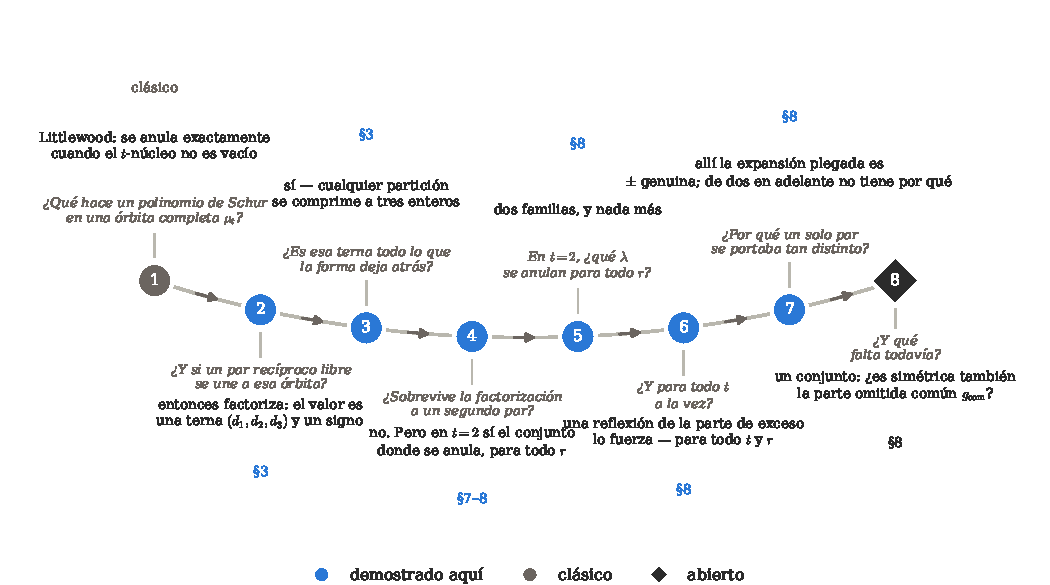
\includegraphics[width=\textwidth]{fig_thread_es.pdf}
\caption{El artículo como un solo hilo. Cada pregunta la responde la perla que tiene debajo, y
cada respuesta es lo que hace que la siguiente pregunta sea la natural: la órbita pide el par
libre, la factorización pide la terna, la terna pide el segundo par, y el segundo par convierte una
fórmula en un lugar. El color distingue lo clásico, lo demostrado aquí y lo que queda abierto, y la
etiqueta bajo cada respuesta es la sección que la resuelve. Dibujada por
\texttt{anc/fig\_intro.py}.}
\label{fig:thread}
\end{figure}

\begin{figure}[!ht]
\centering
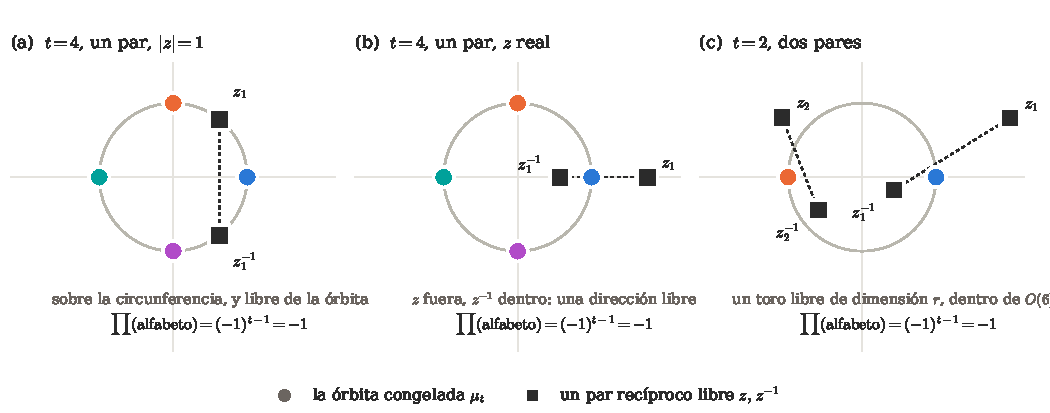
\includegraphics[width=\textwidth]{fig_alphabet_es.pdf}
\caption{El alfabeto, en el plano complejo. La órbita $\mu_t$ está congelada ---un $t$-gono
regular sobre la circunferencia unidad, coloreado por residuo--- y cada par recíproco es una
dirección compleja libre, dibujada unida por un segmento discontinuo. \emph{(a)} el par puede estar
sobre la circunferencia; es una variable libre y no parte de la órbita, y salvo para finitos $z$ no
toca $\mu_t$, que es la razón de que un operador hecho para órbitas de $\zeta$ no tenga nada que
decir de él. \emph{(b)} fuera de la circunferencia, $z$ por fuera y $z^{-1}$ por dentro. \emph{(c)}
$r$ pares dan un toro libre de dimensión $r$. En todos los casos el alfabeto es cerrado por
inversión, así que es la lista de valores propios de un elemento de $O(N,\CC)$ ---el panel (b)
muestra por qué el grupo tiene que ser el complejo--- y el producto de sus letras vale $\zeta^{t(t-1)/2}=(-1)^{t-1}$: para $t$ par esa matriz
está en la componente no identidad. Calculada por \texttt{anc/fig\_intro.py}.}
\label{fig:alphabet}
\end{figure}


Una partición puede ser arbitrariamente grande, y un alfabeto de $N=t+2$ letras sólo alcanza a ver
una parte de ella. Este artículo resuelve, para un alfabeto, exactamente cuánta. El conjunto
completo de las raíces $t$-ésimas de la unidad junto con un par recíproco libre ve un multiconjunto
de tres enteros y un signo, y nada más en absoluto: dos particiones de cualesquiera tamaños que
coincidan en ese dato toman ahí el mismo valor. La forma cerrada del Teorema \ref{thm:main} es cómo
lo demostramos, y la compresión es la parte que esperamos que sobreviva a la fórmula.

La evaluación de polinomios de Schur en raíces de la unidad es clásica y notablemente limpia.
Littlewood y Richardson \cite{LR34} demostraron que $s_\lambda$ se especializa a $0$ o $\pm1$ cuando
las variables se toman como todas las raíces $t$-ésimas de la unidad, siendo el signo un signo de
ordenación y estando la anulación gobernada por el $t$-núcleo de $\lambda$; y en el mismo trabajo lo
generalizaron a un alfabeto que lleva una variable libre en cada letra. Este último resultado fue
redescubierto por Prasad \cite{Pra16}, recibió una nueva demostración de Karmakar \cite{Kar22}, fue
extendido a todos los grupos clásicos por Ayyer y Kumari \cite{AK22} ---quienes además identificaron
el trabajo anterior, casi inadvertido, de Lecouvey \cite{Lec09}--- y fue llevado a los caracteres
universales por Albion \cite{Alb23}. Kumari \cite{Kum24} amplió la familia, Karmakar \cite{Kar24}
trató los elementos de orden dos, Ayyer y Kumari \cite{AK25} añadieron varias especializaciones más,
y Albion \cite{Alb25} relacionó las factorizaciones con las particiones $z$-asimétricas y el
plethysm. Sathish Kumar \cite{SK23} llevó la factorización a las formas sesgadas con
banderas, donde produce una familia de caracteres de Demazure; allí se exige que las banderas
sean múltiplos de $t$, que es la misma demanda de estructura de raíces de la unidad con otro
disfraz. Leída en conjunto, esa línea hace algo más que acumular casos. El enunciado migra de un
grupo a un alfabeto: una vez que los caracteres son universales, evaluar uno es una pregunta sobre
qué letras se escriben, y los tipos clásicos dejan de ser teoremas separados ---el Teorema 5.3 de
\cite{AK25} es un solo enunciado para $s$, $sp$ y $o$ a la vez---. Esa migración es lo que vuelve
formulable la pregunta de este artículo, porque el alfabeto de abajo no pertenece a ningún grupo de
la lista; y las herramientas que tomamos prestadas en la \S\ref{sec:zeros} son las que esa migración
produjo. Remitimos a Albion \cite{Alb23} para un recorrido de toda la línea.

Leído por su \emph{valor}, el teorema de Littlewood es una factorización. Leído por sus \emph{ceros}
es otra cosa ---una clasificación de las $\lambda$ que mueren en un elemento de orden $t$--- y esa
segunda lectura tiene un descendiente propio, que conviene nombrar aquí porque la
\S\ref{sec:zeros} resulta ser su prima. Prasad \cite[Teorema 2]{Pra16} plantea la pregunta de la
anulación no en un punto sino a lo largo de toda una familia: sobre la componente no identidad de
$GL_m^n\rtimes\ZZ/n$ determina cuándo el carácter es idénticamente cero \emph{como función del
parámetro libre}, y la respuesta se lee otra vez en las clases de residuos de $\lambda+\delta$
---cada clase tiene que estar representada exactamente $m$ veces---. En $m=1$ eso es la condición de
Littlewood. Así que un teorema de 1934 tiene dos descendientes, y se separan en qué se permite
que siga libre: allí, órbitas completas de raíces de la unidad; aquí, como veremos, una sola órbita
congelada junto con direcciones \emph{recíprocas} libres. Ninguno de los dos enunciados contiene al
otro.

Una segunda línea de resultados de factorización trata alfabetos cerrados bajo $x\mapsto x^{-1}$.
Okada \cite{Oka98} y Ciucu--Krattenthaler \cite{CK09} trataron las formas rectangulares; Behrend,
Fischer y Konvalinka, y Ayyer, Behrend y Fischer, las escaleras dobles ---para las que seguimos las
atribuciones que da \cite{AB19}---; y Ayyer--Behrend \cite{AB19} las formas autoduales, con
demostraciones biyectivas de estas últimas debidas a Ayyer y Fischer \cite{AF20}. Allí el rédito es
enumerativo: las factorizaciones producen fórmulas de producto para clases de simetría de particiones
planas y para teselaciones de rombos. Las formas autocomplementarias de \cite{AB19} reaparecen en la
\S\ref{sec:zeros} por el otro lado: añadir la letra $-1$ cambia el determinante del alfabeto de $+1$
a $-1$, y las formas que allí factorizan son exactamente las que aquí se anulan.

Las dos líneas nunca han compartido alfabeto, y el obstáculo es estructural en ambas direcciones. El
motor de la primera es un operador ---la Verschiebung $\varphi_t$, en la formulación de Albion
\cite{Alb23}, que actúa sobre los caracteres universales por $\varphi_t h_r=h_{r/t}$ si $t\mid r$ y
$0$ en otro caso--- que exige que el alfabeto sea unión de $\zeta$-órbitas; toda extensión de esa
línea añade por tanto \emph{más} estructura de raíces de la unidad, nunca menos. El motor de la
segunda exige que el alfabeto sea enteramente recíproco, o que la forma sea autocomplementaria. Un
par recíproco libre no es una $\zeta$-órbita, y una órbita de raíces de la unidad no es unión de
pares libres.

La palabra \emph{más pequeño} de abajo puede precisarse, y es el cierre por inversión quien lo
permite. Una extensión de $\zt$ cerrada por inversión solo puede adjuntar pares recíprocos
$\{x,x^{-1}\}$ y los puntos fijos de la inversión, que son $1$ y $-1$; ahora bien, $1$ está en $\zt$
para todo $t$, y $-1$ está en $\zt$ exactamente cuando $t$ es par. La única extensión menor que un
par es por tanto $\zt\cup\{-1\}$ con $t$ impar, y está congelada: sobre $t=3,5,7$ y
$|\lambda|\le14$, las $1092$ formas, $s_\lambda(\zt,-1)$ solo toma los valores $0$ y $\pm1$, sin
nada de lo que pueda depender. Un par recíproco libre es la extensión más pequeña que deja algo que
evaluar.

En este artículo tomamos el alfabeto más pequeño que contiene una letra de cada clase,
\begin{equation}\label{eq:object}
\Phi_t(\lambda;z)\;:=\;s_\lambda\bigl(\,\underbrace{1,\zeta,\dots,\zeta^{t-1}}_{\zt},\;z,\;z^{-1}\bigr),
\qquad \zeta=e^{2\pi i/t},
\end{equation}
un polinomio de Schur en $N=t+2$ variables.

Descrito así, \eqref{eq:object} es un compromiso entre dos líneas, que es como lo encontramos. Se
describe mejor como un solo objeto, y esa descripción es la que reaparece en cada sección de abajo:
\eqref{eq:object} es \emph{un elemento del toro de $O(N)$ con una única dirección libre}. Es cerrado
por inversión, de modo que ya vive donde vive la segunda línea; su determinante es $(-1)^{t+1}$, y
ese determinante es lo que separa factorizar de anularse en la \S\ref{sec:zeros}; la $\zeta$-órbita
es lo que lo coloca en la componente no identidad cuando $t$ es par, donde un carácter es un carácter
entrelazado, que es la Observación \ref{rem:twining}; y el único par libre es la única variable que
sobrevive a la enumeración con signo de la \S\ref{sec:enum}. Los tres resultados de este artículo son
tres lecturas de esa frase.

Nuestro resultado principal, el Teorema \ref{thm:main},
lo evalúa para todo $t$ y toda $\lambda\in\PP_N$ ---toda partición con a lo sumo $N$ partes, sin
restricción alguna sobre su forma ni su tamaño---. Escribimos $\beta=\beta(\lambda,N)$ para la partición
desplazada y $n_i(\lambda)$ para el número de partes de $\beta$ congruentes con $i$ módulo $t$, como
en \cite{AK22}. Puesto que hay $t$ clases de residuos y $N=t+2$ partes, $\sum_i(n_i-1)=2$; luego o
alguna clase está vacía, o, estando todas ocupadas, el exceso sobre una cada una es exactamente dos,
y solo se dan tres perfiles: algún $n_i$ se anula, o dos clases tienen tamaño dos, o una clase tiene
tamaño tres. En el primer caso $\Phi_t=0$; en los otros dos, si $A=\{a_1>a_2\}$ y $B=\{b_1>b_2\}$
denotan las dos clases distinguidas y
\[
d_1=a_1-a_2,\qquad d_2=b_1-b_2,\qquad
\tilde d_3=a_1+a_2-b_1-b_2,\qquad d_3=|\tilde d_3| ,
\]
entonces $\Phi_t=0$ si el \emph{acoplamiento orientado} $\tilde d_3$ se anula, y en otro caso, con
$z=e^{\theta}$,
\[
\boxed{\;\;\Phi_t(\lambda;z)\;=\;\varepsilon_\lambda\,
\frac{\sinh(d_1\theta/2)\,\sinh(d_2\theta/2)\,\sinh(d_3\theta/2)}
{\sinh^2(t\theta/2)\,\sinh\theta}\;\;}
\]
con $\varepsilon_\lambda=\pm1$ dado explícitamente. \emph{Tres factores, nunca más, y sin ninguna
hipótesis sobre la forma de $\lambda$.} Retirado el par recíproco, el enunciado degenera en el de
Littlewood, de modo que el contenido es lo que ese par añade: exactamente un término de
acoplamiento, a saber $d_3$. Leído con caracteres $\mathfrak{sl}_2$ el mismo enunciado no lleva
exponencial ninguna: es el producto triple $\chi_{d_1/2-1}\chi_{d_2/2-1}\chi_{d_3/2-1}$ sobre
$\chi_{t/2-1}^2$, uniformemente en $t$ (Corolario \ref{cor:chars}), con índices semienteros
exactamente cuando $t$ es impar.

El alfabeto es un solo objeto, y la respuesta también. El perfil de residuos, la terna
$(d_1,d_2,d_3)$ y el signo son todo lo que el teorema necesita, y en la \S\ref{sec:main} los
reunimos en un único \emph{invariante de la evaluación} $I_t(\lambda)$, \eqref{eq:invariant}, a
través del cual el valor factoriza. Es completo pero no mínimo: \eqref{eq:main} es simétrica en los
tres enteros, de modo que lo que se ve es el multiconjunto y el signo, que es la compresión
anunciada arriba. Lo que \emph{no} se ve es entonces una pregunta bien planteada. La
\S\ref{sec:fibrelattice} la responde para los tres enteros ---las particiones que los comparten
forman un retículo, y escribimos su función generatriz--- y lo que el signo añade a eso es el
Problema \ref{prob:fibres}.

Los tres enteros admiten una lectura que vuelve transparente la fórmula, y la damos aquí porque es
como pensamos el resultado. Considérense $A$ y $B$ como intervalos $[a_2,a_1]$ y $[b_2,b_1]$ sobre la
recta beta. Entonces
\begin{equation}\label{eq:intervals}
d_1=|A|,\qquad d_2=|B|,\qquad d_3=2\,\bigl|\mathrm{centro}(A)-\mathrm{centro}(B)\bigr| :
\end{equation}
\emph{las dos longitudes, y el doble de la distancia entre los centros} (Figura
\ref{fig:intervals}). El criterio de anulación se vuelve geométrico ---una clase de residuos es
vacía, o los dos intervalos son concéntricos--- y explica de inmediato por qué el perfil de tamaño
tres, donde los intervalos comparten un extremo, nunca se anula. Los intervalos concéntricos
resultan exigir $t$ par (Proposición \ref{rem:lattice}), de modo que para $t$ impar una clase de
residuos vacía es la única forma de anularse ---y eso sigue siendo cierto para cualquier número de
pares recíprocos, que es el Corolario \ref{cor:oddgen}---. Equivalentemente, en el idioma de la
primera línea, $d_1$ y $d_2$ son $t$ veces los contenidos $\mathfrak{sl}_2$ de las dos componentes
distinguidas del cociente, y el acoplamiento orientado $\tilde d_3$ es un funcional \emph{afín} sobre
el vector de \emph{tamaños} del cociente, entrando los dos residuos como un desplazamiento, con
$d_3=|\tilde d_3|$ (Proposición \ref{prop:quotient}). No es
un funcional sobre el vector de residuos, y por tanto tampoco sobre el retículo de raíces de tipo
$A_{t-1}$ bajo la correspondencia de Garvan--Kim--Stanton \cite{GKS90}: ya en $t=2$ el único perfil
de dos clases lleva diez valores distintos de $d_3$ sobre $|\lambda|\le16$. En qué mitad de la
descomposición núcleo--cociente vive cada cláusula del criterio de anulación queda resuelto en la
Proposición \ref{rem:lattice}.

Se siguen dos consecuencias. El Teorema 5.3 de \cite{AK25} determina cuándo un carácter universal es
independiente de las variables por las que se le tuerce, uniformemente en los tres tipos clásicos, y
leído sobre \eqref{eq:object} diría que
$s_\lambda(z,z^{-1},\zt)=s_\lambda(z,z^{-1})$ exactamente sobre los $t$-núcleos, para
$\ell(\lambda)\le2$. Ese criterio está enunciado para variables libres, y un par recíproco no lo es;
sobre ese lugar aparece una familia más, y el Teorema \ref{thm:extra} la clasifica por su núcleo y su cociente. En
\S\ref{sec:enum} leemos la identidad como una enumeración: una fórmula de producto para un recuento
de tablas semiestándar pesado por raíces de la unidad en el que el parámetro $z$ sigue libre, y en
$t=2$ una $(-1)$-enumeración de particiones planas en una caja refinada por $z$.

Las dos últimas secciones hacen una pregunta distinta, no sobre lo que la identidad da sino sobre
hasta dónde alcanza. La \S\ref{sec:sharp} prueba cuatro deformaciones naturales del alfabeto, cada
una de las cuales destruye la identidad, y una sola lectura de la demostración explica las
cuatro. Luego la
\S\ref{sec:zeros} aísla lo que sí sobrevive. Añadir más pares recíprocos cuesta la fórmula de
producto del Teorema \ref{thm:main}, pero
no el \emph{lugar de anulación}: para todo número $r$ de pares, el carácter
$s_\lambda(1,-1,z_1,\bar z_1,\dots,z_r,\bar z_r)$ se anula exactamente cuando el conjunto beta tiene
paridad constante o $\lambda$ es autocomplementaria de anchura impar (Teorema \ref{conj:crit}).
Leído sobre el grupo y no sobre el alfabeto, el mismo enunciado es una clasificación: ésas son
exactamente las $\lambda$ cuyo $GL(N)$-módulo restringe a $O(N)$ de forma estable bajo el giro por
$\det$ (Corolario \ref{cor:dettwist}). Las formas son las autocomplementarias de \cite{AB19}, donde el mismo
alfabeto sin la letra $-1$ hace que el carácter factorice en lugar de anularse; el determinante del
alfabeto decide cuál de las dos cosas pasa. La dirección suficiente es un corolario corto de la
complementación y lo decimos así; el contenido es el recíproco, que demostramos para todo $r$ y toda
$\lambda$, módulo un teorema de rigidez para productos de polinomios de Schur.

Conviene dibujar el mapa, y la Figura \ref{fig:plane} lo es. Adjuntar $r$ pares recíprocos a la
órbita $\zt$ da una familia en los dos parámetros $(t,r)$, y el lugar de anulación está resuelto en
tres partes de ella --- una fila, una columna, y todas las columnas impares, que son medio plano.

\begin{figure}[!ht]
\centering
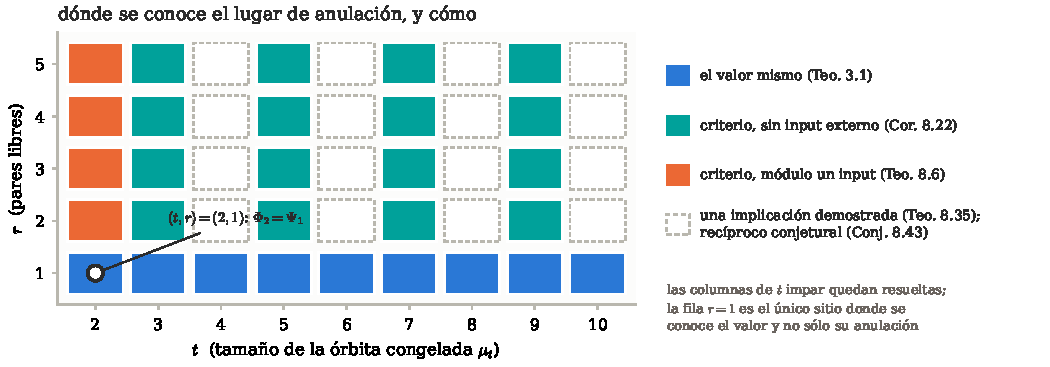
\includegraphics[width=\textwidth]{fig_plane_es.pdf}
\caption{La familia de dos parámetros, y lo que se sabe sobre ella. Cada celda es un alfabeto
$\zt\cup\{z_1^{\pm1},\dots,z_r^{\pm1}\}$; el color no se asigna a mano, sino que se calcula a partir
de los propios enunciados, con una regla por línea del artículo. La fila $r=1$ es el único sitio
donde se conoce el \emph{valor} y no sólo su anulación, que es el Teorema \ref{thm:main}; las
columnas de $t$ impar las resuelve el Corolario \ref{cor:oddgen} sin ningún input externo; la columna
$t=2$, el Teorema \ref{conj:crit}, que usa uno. En las celdas restantes el Teorema \ref{thm:suff}
prueba una implicación y la Conjetura \ref{conj:general} es la otra. La esquina marcada es donde se
encuentran las dos mitades del artículo: allí $\Phi_2=\Psi_1$, y es el único alfabeto que ven las
dos. Calculada por \texttt{anc/fig\_plane.py}.}
\label{fig:plane}
\end{figure} El Teorema \ref{thm:main}
es $r=1$: un par, todo $t$, y ahí tenemos el valor y no sólo su anulación.
El Teorema \ref{conj:crit} es $t=2$: cualquier número de pares, la órbita más pequeña. Y el Corolario
\ref{cor:oddgen} es \emph{todo $t$ impar y todo $r$} a la vez: allí el carácter se anula si y sólo si
falta una clase de residuos, de modo que la rama concéntrica es un fenómeno exclusivo de $t$ par. La
tercera de las tres no es un borde sino medio plano, y es además la más barata --- sale del argumento
extremal de la \S\ref{sec:extremal} sin ningún input externo, mientras que la segunda necesita el
Teorema \ref{thm:PvW}. Fuera de esas tres regiones el lugar no está resuelto, pero ya no está intacto. El
Teorema \ref{thm:suff} da una condición sobre el conjunto beta --- una reflexión de su parte de
exceso, y un incremento que da en el centro --- que fuerza la anulación del carácter para
\emph{todo} $t$ y todo $r$, mediante una involución que empareja todos los términos del desarrollo;
el Corolario \ref{cor:necgen} da una condición necesaria por el otro lado. Que las dos se encuentren
es la Conjetura \ref{conj:general}, y lo que las separa es una sola implicación, que la
\S\ref{sec:rigidity} muestra que no puede venir del estrato en el que ese argumento trabaja. El
fórmula de producto del Teorema \ref{thm:main} ya falla en $r=2$, por (D1) ---que no exista tal
fórmula para ningún $r\ge2$ es la Conjetura \ref{conj:rank2}, y no algo que demostremos---, así que
pasada la línea $r=1$ el lugar es lo que podemos ofrecer.

Hay algo que el alfabeto delata y que merece decirse aquí y no de pasada. Tiene una lectura en
teoría de representaciones ---de la clase que \cite{CK09} registran como ausente para sus
factorizaciones, y con ellos \cite{AB19} y \cite{AK25}--- y el mecanismo no es nuestro: el alfabeto
es cerrado por inversión, luego
un elemento del toro de $O(N)$ de determinante $(-1)^{t+1}$, de modo que para $t$ par vive en la
componente no identidad, donde un carácter es un carácter \emph{entrelazado} en el sentido de
Jantzen \cite{Jantzen} y Kumar--Lusztig--Prasad \cite{KLP} y el plegado lo da el álgebra de Lie de
órbitas. La Observación \ref{rem:twining} lo precisa y el Lema \ref{lem:AtoSp} lo concreta ---allí el
álgebra plegada es $C_r$ y el carácter entrelazado es un carácter simpléctico sin más. La
demostración del Teorema \ref{thm:main} no usa nada de eso, y por eso lo enunciamos como lectura y no
como método.

El artículo se organiza como sigue. Fijamos notación y recordamos las dos evaluaciones sobre las que
construimos en la Sección \ref{sec:background}. En la Sección \ref{sec:main} enunciamos el teorema
principal, identificamos sus tres enteros en términos del núcleo y del $t$-cociente, describimos las
particiones que no consiguen separar y registramos el criterio de
anulación y la imagen de la aplicación resultante. La Sección \ref{sec:proof} contiene la
demostración. En la Sección \ref{sec:independence} comparamos el teorema con el criterio de
independencia de \cite{AK25} y determinamos la familia adicional que adquiere en el lugar recíproco.
En la Sección \ref{sec:enum} leemos el teorema como una enumeración y ensamblamos, en $t=2$, la
involución que invierte el signo que esa enumeración pide, y en la Sección
\ref{sec:sharp} probamos cuatro deformaciones del alfabeto, cada una de las cuales destruye la
identidad. La Sección \ref{sec:zeros} determina
el lugar de anulación en $t=2$ para un número arbitrario de pares recíprocos ---y, sin ningún coste
externo, también en todo $t$ impar---, lee ese criterio sobre el grupo como una rigidez frente al
giro por el determinante, y da un criterio suficiente, con recíproco conjetural, para $t$ y $r$
arbitrarios. La Sección \ref{sec:verif} recoge las
comprobaciones numéricas y la Sección \ref{sec:open} los problemas abiertos.

%======================================================================
\section{Preliminares y notación}\label{sec:background}

Seguimos la notación de \cite{AK22,AK25}. Todos los grupos algebraicos son aquí sobre $\CC$; en
particular $O(N)$ significa $O(N,\CC)$, que es lo que da un alfabeto cerrado por $x\mapsto x^{-1}$
cuando se permite a sus letras salir de la circunferencia unidad.

\subsection{Particiones, conjuntos beta, núcleos y cocientes}
Una partición $\lambda=(\lambda_1,\dots,\lambda_n)$ es una sucesión débilmente decreciente de enteros
no negativos; $\PP_n$ denota el conjunto de particiones de longitud a lo sumo $n$, $|\lambda|$ el
tamaño y $\ell(\lambda)$ la longitud. En todo el texto $t\ge2$ es un entero fijo, $\zeta$ una raíz
$t$-ésima primitiva de la unidad, $\zt=\{1,\zeta,\dots,\zeta^{t-1}\}$, y
\[
N:=t+2 .
\]
Para $\lambda\in\PP_N$ el \emph{conjunto beta} es $\beta(\lambda)=(\beta_1,\dots,\beta_N)$ con
$\beta_j=\lambda_j+N-j$, de modo que $\beta_1>\beta_2>\dots>\beta_N\ge0$; indexamos por
\emph{columnas} $j=1,\dots,N$, y observamos que un $\beta$ mayor significa un índice de columna menor.
Para $0\le i\le t-1$ escribimos $n_i(\lambda)$ para el número de partes de $\beta(\lambda)$
congruentes con $i$ módulo $t$, de manera que
\begin{equation}\label{eq:excess}
\sum_{i=0}^{t-1}n_i(\lambda)=N=t+2 .
\end{equation}
Llamamos \emph{perfil de residuos} de $\lambda$ al vector
$\bigl(n_0(\lambda),\dots,n_{t-1}(\lambda)\bigr)$. Por \eqref{eq:excess},
$\sum_i\bigl(n_i(\lambda)-1\bigr)=2$: o alguna clase está vacía, o, estando todas ocupadas, el
exceso sobre una cada una es exactamente dos, y sólo hay dos particiones de dos. De modo que un
perfil es de exactamente uno de tres tipos: \emph{degenerado}, si algún $n_i=0$; \emph{de dos
clases}, si dos entradas valen $2$; o \emph{de tamaño tres}, si una entrada vale $3$. Todo lo que
sigue en este artículo está gobernado por cuál de los tres se da.
Sea $\sigma\in S_N$ la permutación que reordena las partes de $\beta(\lambda)$ agrupándolas por clase
de residuo, con las clases en orden creciente y los valores dentro de cada clase en orden
decreciente; es la permutación de \cite[(2.1)]{AK25}. Escribimos $\core_t(\lambda)$ y
$\quot_t(\lambda)=(\lambda^{(0)},\dots,\lambda^{(t-1)})$ para el $t$-núcleo y el $t$-cociente,
definidos a partir de $\beta(\lambda)$ como en \cite[\S2.1]{AK25}. Por \cite{GKS90}, los $t$-núcleos
están en biyección con los vectores del retículo de raíces de tipo $A_{t-1}$, y los recuentos de
residuos $n_i$ son las coordenadas naturales.

Ponemos $\zb:=z^{-1}$, $z=e^{\theta}$, y abreviamos
\[
f(u):=z^{u}-z^{-u}=2\sinh(u\theta),\qquad
V:=\prod_{0\le k<k'\le t-1}\bigl(\zeta^{k'}-\zeta^{k}\bigr).
\]
Para un conjunto $S$ de columnas, $b_S$ es la palabra de residuos $\beta_j\bmod t$ para $j\in S$
leída en orden creciente de columna, e $\inv(b_S)$ su número de inversiones. Usamos el bialternante
\[
s_\lambda(x_1,\dots,x_N)=\frac{\det\bigl(x_i^{\beta_j}\bigr)_{i,j=1}^N}
{\det\bigl(x_i^{N-j}\bigr)_{i,j=1}^N}.
\]

\subsection{Las dos evaluaciones sobre las que construimos}
Recordamos los dos enunciados entre los que se sitúa el presente resultado. El primero es la
evaluación de Littlewood, en la forma de \cite[Teorema 2.2]{AK25}.

\begin{theorem}[{\cite[Teorema IX]{LR34}}]\label{thm:LR}
Sea $\lambda\in\PP_t$. Entonces
\[
s_\lambda(1,\zeta,\dots,\zeta^{t-1})=
\begin{cases}
(-1)^{\binom{t}{2}}\sgn(\sigma) & \text{si }\core_t(\lambda)=\varnothing,\\
0 & \text{en otro caso.}
\end{cases}
\]
\end{theorem}

El segundo es el criterio de independencia que extendemos, \cite[Teorema 5.3]{AK25}; enunciamos el
caso que necesitamos. Sea $f_\lambda$ un carácter universal de tipo $s$, $sp$ u $o$, sea $Y$ un
conjunto de $m$ variables y sean $x_1,\dots,x_{n-tm}$ libres. Entonces
\begin{equation}\label{eq:AK53}
f_\lambda(x_1,\dots,x_{n-tm},Y,\zeta Y,\dots,\zeta^{t-1}Y)=f_\lambda(x_1,\dots,x_{n-tm})
\quad\Longleftrightarrow\quad \lambda=\core_t(\lambda),
\end{equation}
para $\lambda\in\PP_{n-tm}$. El criterio es uniforme en el tipo ---un solo enunciado para $s$, $sp$ y
$o$ a la vez---, que es lo que lo hace citable aquí: nuestro alfabeto es un alfabeto de $GL$, y lo
que le preguntamos es una cuestión sobre una especialización y no sobre un grupo. Tomando $m=1$,
$Y=(1)$ y $(x_1,x_2)=(z,\zb)$ se obtiene $n=t+2$ y nuestro alfabeto, pero esa sustitución es
justamente donde se abandona la hipótesis de que $x_1,x_2$ sean libres. Así que \eqref{eq:AK53} no se
está aplicando sobre el lugar recíproco; se le está preguntando por él, que es la
\S\ref{sec:independence}.

\begin{remark}\label{rem:notacase}
El enunciado más próximo de la literatura añade dos letras extra, igual que nosotros, de modo que
conviene registrar por qué no contiene \eqref{eq:object}. Kumari \cite[Teorema 2.2]{Kum24} evalúa
$s_\lambda(X,\zeta X,\dots,\zeta^{t-1}X,\,y,\zeta y,\dots,\zeta^{m-1}y)$; con $X=(1)$ y $m=2$ el
bloque añadido es $\{y,\zeta y\}$, mientras que el nuestro es $\{z,z^{-1}\}$. Los dos coinciden solo
cuando $z^{2}=\zeta^{\pm1}$, un conjunto finito de puntos y no una variable libre. Lo mismo vale para
la única variable libre extra de \cite[Teorema 2.7]{AK22} y para el Teorema XI de
Littlewood--Richardson.
\end{remark}

%======================================================================
La Figura \ref{fig:beta} hace todo el diccionario sobre una forma concreta.

\begin{figure}[!ht]
\centering
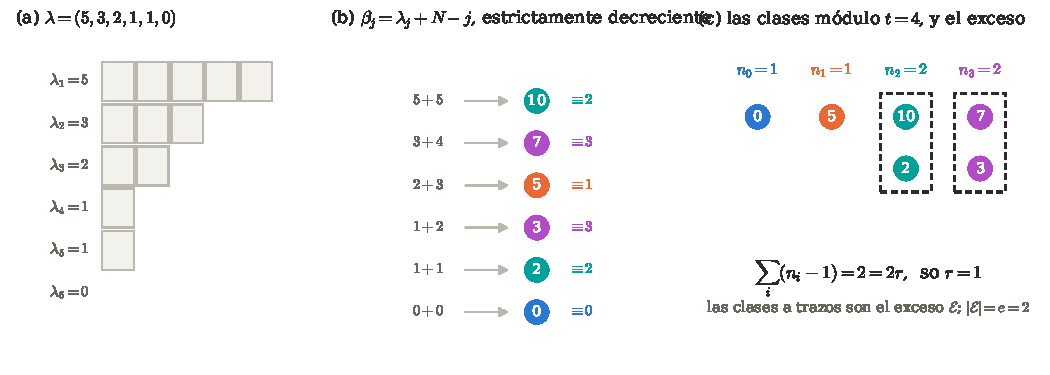
\includegraphics[width=\textwidth]{fig_beta_es.pdf}
\caption{El diccionario sobre el que corre el resto del artículo, con $\lambda=(5,3,2,1,1,0)$ y
$t=4$. \emph{(a)} la forma, rellenada hasta $N$ partes. \emph{(b)} $\beta_j=\lambda_j+N-j$, que
convierte una sucesión débilmente decreciente en una estrictamente decreciente y por tanto en un
conjunto; cada valor se colorea después según su residuo módulo $t$. \emph{(c)} el perfil de
residuos $(n_0,\dots,n_{t-1})$ y el recuento \eqref{eq:excess}: $\sum_i(n_i-1)=2r$ siempre, de modo
que cuando toda clase está ocupada las clases con $n_i\ge2$ ---el exceso $\mathcal{E}$, a trazos---
llevan exactamente $2r$ elementos más de uno cada una. Si alguna está vacía la suma sigue valiendo
$2r$ pero ya no es un exceso: ésa es la rama degenerada, que se resuelve la primera.
Todo lo que el artículo demuestra es un enunciado sobre ese dibujo.
Calculada por \texttt{anc/fig\_intro.py}.}
\label{fig:beta}
\end{figure}

\section{La evaluación}\label{sec:main}

\keybox{\emph{El teorema en una frase.} El valor depende de $\lambda$ a través de su perfil de
residuos, una terna de intervalos $(d_1,d_2,d_3)$ y un signo, y de nada más: una partición
arbitrariamente grande queda comprimida a tres enteros y un signo.}

\begin{theorem}\label{thm:main}
Sean $t\ge2$ y $\lambda\in\PP_N$, con $N=t+2$.
\begin{enumerate}
\item[\rm(i)] Si $n_i(\lambda)=0$ para algún $i$, entonces $\Phi_t(\lambda;z)=0$.
\item[\rm(ii)] En caso contrario, por \eqref{eq:excess}, o bien exactamente dos clases de residuos
tienen $n_i=2$, o bien exactamente una tiene $n_i=3$. Sean $r_A\le r_B$ los residuos implicados y
sean
\[
A=\{a_1>a_2\},\qquad B=\{b_1>b_2\}
\]
en el primer caso las partes de $\beta(\lambda)$ en las clases $r_A$ y $r_B$, y en el segundo los dos
pares solapados $A=\{p,q\}$, $B=\{q,r\}$ de la clase $\{p>q>r\}$, de modo que $r_A=r_B$. Pongamos
\[
d_1=a_1-a_2,\qquad d_2=b_1-b_2,\qquad
\tilde d_3=a_1+a_2-b_1-b_2,\qquad d_3=|\tilde d_3| ,
\]
y llamemos a $\tilde d_3$ el \emph{acoplamiento orientado}. Si $\tilde d_3=0$, entonces
$\Phi_t(\lambda;z)=0$. En caso contrario, con $z=e^\theta$,
\begin{equation}\label{eq:main}
\boxed{\;\;\Phi_t(\lambda;z)\;=\;\varepsilon_\lambda\cdot
\frac{\sinh(d_1\theta/2)\,\sinh(d_2\theta/2)\,\sinh(d_3\theta/2)}
{\sinh^2(t\theta/2)\,\sinh\theta}\;\;}
\end{equation}
donde, escribiendo $j_{A_1}$ y $j_{B_1}$ para las columnas que llevan $a_1$ y $b_1$, $S$ para el
complementario de $\{j_{A_1},j_{B_1}\}$ en $\{1,\dots,N\}$, y $b_S$ para la palabra de residuos de
$\beta(\lambda)$ sobre $S$ leída en orden creciente de columna,
\begin{equation}\label{eq:sign}
\varepsilon_\lambda\;=\;(-1)^{\,t+\binom{N+1}{2}}\;
(-1)^{\,j_{A_1}+j_{B_1}+\inv(b_S)}\;\sgn(a_1-b_1)\;\sgn(\tilde d_3).
\end{equation}
\end{enumerate}
Cada uno de los cuatro factores es $\pm1$ ---el último porque $\tilde d_3\ne0$ es exactamente la
hipótesis de {\rm(ii)}---, luego $\varepsilon_\lambda=\pm1$. En el perfil de tamaño tres $r_A=r_B$ y
$\tilde d_3=p-r>0$, luego ese factor es $+1$.

El lado izquierdo es un polinomio de Laurent en $z$. Leemos \eqref{eq:main} como identidad en
$\CC(z)$; tras la cancelación el lado derecho es también un polinomio de Laurent, y en los ceros del
denominador ---$z=\pm1$ y $z^t=1$--- usamos esa continuación. Así lo hacemos en \S\ref{sec:enum},
donde el valor se toma en $z=1$.
\end{theorem}

\noindent Separar $d_3$ en su tamaño y su orientación no es contabilidad. El signo \eqref{eq:sign}
necesita la orientación y la fórmula necesita solo el tamaño, y en $\tilde d_3=0$ la orientación no
existe: un enunciado que lleve $\sgn(a_1+a_2-b_1-b_2)$ y afirme que vale $\pm1$ es falso sobre el
lugar concéntrico, donde ese argumento es cero. El valor allí es $0$ por el factor
$\sinh(d_3\theta/2)$, de modo que nada de lo que viene después cambia; lo que cambia es que el caso
queda ahora excluido antes de escribir el signo, y no después.

Escribimos
\[
d(\lambda):=(d_1,d_2,d_3)
\]
y lo llamamos la \emph{terna de intervalos} de $\lambda$, siguiendo la lectura
\eqref{eq:intervals}; y llamamos a $d_3$ el \emph{término de acoplamiento}, por ser el único de los
tres que mezcla las dos clases distinguidas.

Conviene dar nombre al dato completo, porque el teorema se lee mejor como un enunciado sobre él que
como una fórmula. Pongamos
\begin{equation}\label{eq:invariant}
\boxed{\;\;I_t(\lambda)\;:=\;\begin{cases}
0 & \text{si el perfil de residuos es degenerado, o }\tilde d_3=0,\\[2pt]
\bigl(d_1,d_2,d_3,\varepsilon_\lambda\bigr) & \text{en otro caso},
\end{cases}\;\;}
\end{equation}
y llamémoslo el \emph{invariante de la evaluación} de $\lambda$. Su primera rama es exactamente el
lugar de anulación del Corolario \ref{cor:zero}, y es una rama y no dos porque en todo él no hay
signo que registrar: \eqref{eq:sign} necesita $\tilde d_3\ne0$. El Teorema \ref{thm:main} dice
entonces dos cosas a la vez. Primera, que $\Phi_t$ \emph{factoriza a través} de $I_t$: la aplicación
$\lambda\mapsto\Phi_t(\lambda;z)$ es la composición de $\lambda\mapsto I_t(\lambda)$ con una función
del invariante solo. Segunda, que ese invariante es \emph{completo} para esta evaluación: si dos
particiones tienen el mismo $I_t$ tienen el mismo $\Phi_t$, sean del tamaño que sean. La completitud
es lo que hace que la compresión anunciada más arriba merezca un nombre y no solo una observación
---dice que el invariante no es un resumen cómodo de la dependencia, sino la dependencia entera--- y
convierte la pregunta natural siguiente, qué olvida el invariante, en una pregunta bien planteada.
La Proposición \ref{prop:minimal} cierra la pregunta por el otro lado: una vez leída la terna como
multiconjunto, tampoco puede suprimirse nada de $I_t$. Así que la \S\ref{sec:fibrelattice} resuelve
qué se olvida para la terna y el Problema \ref{prob:fibres} es lo que deja
el signo. Los $(d_1,d_2,d_3)$ de la Figura \ref{fig:image} son
los valores que toma este invariante, dibujados.

Esa factorización es una sola tubería, y cada flecha pierde información que ya no vuelve:
% multline y no \[...\]: la cadena entera no cabe en una caja de 436 pt, y una formula sin puntos
% de corte no se parte sola.  El corte va tras el paso que pierde los intervalos, que es donde el
% lector para de todos modos.
\begin{multline*}
\lambda\;\longrightarrow\;\beta(\lambda)\;\longrightarrow\;
\bigl(\text{perfil de residuos},\ \text{los dos intervalos distinguidos}\bigr)\\
\longrightarrow\;\bigl(d_1,d_2,d_3,\varepsilon_\lambda\bigr)\;\longrightarrow\;\Phi_t(\lambda;z).
\end{multline*}
Los intervalos hay que llevarlos junto al perfil: el perfil dice qué clases son las distinguidas y
nada sobre dónde caen sus números beta, de modo que no determina la terna.
Coordenada a coordenada, el invariante reparte el trabajo así.

\begin{center}\small
\begin{tabular}{ll}
\toprule
dato de $\lambda$ & qué controla\\
\midrule
perfil de residuos & la rama degenerada de anulación\\
las dos longitudes $d_1,d_2$ & los dos primeros factores\\
la distancia entre los centros, $d_3$ & el factor de acoplamiento, y la rama concéntrica de anulación\\
la orientación $\sgn(\tilde d_3)$ & un factor del signo\\
el signo de ordenación $\varepsilon_\lambda$ & el signo global\\
\bottomrule
\end{tabular}
\end{center}

\noindent Ninguna de las dos ramas de anulación es la otra: el perfil no puede ver la concéntrica, y
la terna no puede ver la degenerada, y por eso el criterio del Corolario \ref{cor:zero} tiene dos
cláusulas y la \S\ref{sec:main} dedica una proposición a decir dónde vive cada una.

\keybox{Un solo recuento recorre el artículo. Con $t$ clases de residuos, $N=t+2$ partes y toda
clase ocupada, el exceso es exactamente dos, de modo que por \eqref{eq:excess} un perfil sólo
puede ser degenerado, de dos
clases o de tamaño tres: esa tricotomía es la forma del Teorema \ref{thm:main}, la
división en casos de su demostración en la \S\ref{sec:proof}, y la primera rama del lugar de
anulación en la \S\ref{sec:zeros}. Dos clases distinguidas son lo que el par recíproco tiene que
acoplar, y de ahí exactamente un término de acoplamiento y tres factores en vez de dos.}

El recuento de tres tiene una segunda explicación, que no debe nada a la demostración. El exceso
dos da dos clases distinguidas, que son dos intervalos sobre la recta beta, y un par de intervalos
son cuatro números $(a_1,a_2,b_1,b_2)$. Los tres argumentos de \eqref{eq:main} ven qué forma tiene
ese par y no dónde está: un desplazamiento común $\beta\mapsto\beta+m$ deja $d_1$, $d_2$ y
$\tilde d_3$ intactos. Así que lo único que puede entrar en ellos es un funcional lineal que mate la
traslación común, y esos forman el hiperplano $\sum\alpha_i=0$ del dual de dimensión cuatro: un
espacio de dimensión exactamente \emph{tres}. La terna $d_1=(1,-1,0,0)$, $d_2=(0,0,1,-1)$ y
$\tilde d_3=(1,1,-1,-1)$ es una base de él. Módulo la traslación común, un par de intervalos tiene
tres coordenadas lineales independientes, y de ahí sale el recuento de tres. Lo que el Teorema
\ref{thm:main} añade, y que el recuento de dimensiones \emph{no} fuerza, es que en esta
especialización esas tres coordenadas \emph{se separan multiplicativamente}: un producto con un
factor de cada una, y no otra función de tres variables.

El \emph{valor} no es invariante por traslación, y merece la pena decirlo, porque lo que es en su
lugar es una restricción sobre el signo. Un desplazamiento $\beta\mapsto\beta+m$ es
$\lambda\mapsto\lambda+(m^N)$, y $s_{\lambda+(m^N)}(A)=\det(A)^{m}s_\lambda(A)$ para cualquier
alfabeto $A$, así que por \eqref{eq:object}
\begin{equation}\label{eq:shift}
\Phi_t\bigl(\lambda+(m^N);z\bigr)\;=\;(-1)^{(t+1)m}\,\Phi_t(\lambda;z).
\end{equation}
Para $t$ impar el valor es invariante; para $t$ par un desplazamiento impar lo invierte. La terna no
se mueve, de modo que toda esa inversión la lleva $\varepsilon_\lambda$ --- lo que convierte a
\eqref{eq:shift} en una comprobación de \eqref{eq:sign} que no cuesta nada y que el signo supera,
sobre las formas de la \S\ref{sec:verif}. Es además la razón de que el lema haya que enunciarlo sobre
la terna y no sobre el valor: para $t$ par el valor no es función de la clase de traslación de la
terna.

El signo \eqref{eq:sign} es un signo de ordenación, de la misma especie que el del Teorema
\ref{thm:LR}; la Proposición \ref{rem:sign} registra más abajo una expresión más corta para él, en la
notación de \cite{AK25}.

El miembro derecho de \eqref{eq:main} es un cociente, y el contenido del teorema es que ese cociente
es un polinomio de Laurent en $z$. Para $t$ impar el factor $\sinh(t\theta/2)$ por separado no es un
monomio de Laurent, de modo que los tres factores no están individualmente en $\ZZ[z,z^{-1}]$; solo
lo está su combinación. Aun así el enunciado es uniforme en $t$.

\begin{corollary}\label{cor:zero}
$\Phi_t(\lambda;z)\equiv0$ si y solo si alguna clase de residuos módulo $t$ es vacía, o
$a_1+a_2=b_1+b_2$. En particular el perfil de tamaño tres nunca se anula.
\end{corollary}

\noindent La anulación es idéntica en $z$, no en un punto: cuando ocurre, $\lambda$ no aporta nada en
ningún elemento de la familia de un parámetro que barre el par recíproco. Ésa es la forma en que se
planteaba la pregunta de Prasad en la \S\ref{sec:background}, y el sentido en que \eqref{eq:object}
se lee fuera de la combinatoria ---siendo la mitad congelada del alfabeto una holonomía de orden
finito, y el par libre lo que queda del toro---.

\begin{corollary}\label{cor:chars}
Escribamos $\chi_k(z)=(z^{k+1}-z^{-k-1})/(z-z^{-1})$ para el carácter del $\mathfrak{sl}_2$-módulo
irreducible de dimensión $k+1$ cuando $k\ge0$ es entero. Para $k$ semientero conservamos la misma
fórmula, leída en $u=z^{1/2}$; es entonces notación y no un carácter, porque los factores por
separado no son de Laurent en $z$. Entonces
\eqref{eq:main} puede escribirse sin ninguna exponencial y sin convenio alguno para $\theta$:
\begin{equation}\label{eq:chiratio}
\boxed{\;\;\Phi_t(\lambda;z)\;=\;\varepsilon_\lambda\,
\frac{\chi_{\frac{d_1}{2}-1}(z)\;\chi_{\frac{d_2}{2}-1}(z)\;\chi_{\frac{d_3}{2}-1}(z)}
{\chi_{\frac{t}{2}-1}(z)^{2}}\;\;}
\end{equation}
Para $t=2$ el denominador es $\chi_0=1$ y todo $d_i$ es par, luego $\Phi_2$ es sin más un producto
con signo de tres caracteres $\mathfrak{sl}_2$. Para $t$ impar los índices son semienteros, que es el
enunciado de arriba en otra forma: los tres factores no son Laurent por separado, y solo lo es el
cociente. Cada factor se lee en $u=z^{1/2}$ y cambia de signo bajo $u\mapsto-u$ exactamente cuando
su índice es semientero; como $d_1+d_2+d_3$ es par ---tiene la paridad de
$d_1+d_2+\tilde d_3=2(a_1-b_2)$---, el cociente no cambia, y es el polinomio de Laurent en $z$ de
\eqref{eq:main}.
\end{corollary}

\begin{proof}
Escribamos $f(u)=z^{u}-z^{-u}=2\sinh(u\theta)$, de modo que $\chi_k=f(k+1)/f(1)$. El numerador de
\eqref{eq:main} es $f(d_1/2)f(d_2/2)f(d_3/2)/8$ y su denominador es $f(t/2)^2f(1)/8$, así que
\eqref{eq:main} vale $\varepsilon_\lambda f(d_1/2)f(d_2/2)f(d_3/2)/\bigl(f(t/2)^2f(1)\bigr)$;
sacando tres factores $f(1)$ del numerador y dos del denominador se obtiene \eqref{eq:chiratio}.
\end{proof}

\subsection{Los tres enteros vienen del cociente}
Lo siguiente identifica $(d_1,d_2,d_3)$ en el idioma de la línea de raíces de la unidad. Para una
partición $\nu$ ponemos $k(\nu)=\nu_1-\nu_2$, su contenido $\mathfrak{sl}_2$.

\begin{proposition}\label{prop:quotient}
En el perfil de dos clases, con $\quot_t(\lambda)=(\lambda^{(0)},\dots,\lambda^{(t-1)})$,
\[
d_1=t\bigl(k(\lambda^{(r_A)})+1\bigr),\qquad
d_2=t\bigl(k(\lambda^{(r_B)})+1\bigr),\qquad
\tilde d_3=t\bigl(|\lambda^{(r_A)}|-|\lambda^{(r_B)}|\bigr)+2(r_A-r_B) .
\]
En el perfil de tamaño tres la única componente distinguida $\lambda^{(r_A)}$ tiene tres partes y
\[
d_1=t\bigl(\lambda^{(r_A)}_1-\lambda^{(r_A)}_2+1\bigr),\quad
d_2=t\bigl(\lambda^{(r_A)}_2-\lambda^{(r_A)}_3+1\bigr),\quad \tilde d_3=d_1+d_2 .
\]
\end{proposition}

\begin{proof}
Escribamos $a_i=t\tilde a_i+r_A$. La clase $r_A$ lleva dos números beta, luego
$\lambda^{(r_A)}=(\tilde a_1-1,\tilde a_2)$ por la definición del cociente, de donde
$k(\lambda^{(r_A)})=\tilde a_1-\tilde a_2-1$ y $d_1=t(\tilde a_1-\tilde a_2)$, que es la primera
identidad; la segunda es el mismo cálculo. Para la tercera, $\tilde a_1+\tilde a_2=|\lambda^{(r_A)}|+1$
y análogamente para $B$, luego $a_1+a_2-b_1-b_2=t(|\lambda^{(r_A)}|-|\lambda^{(r_B)}|)+2(r_A-r_B)$. El
caso de tamaño tres es idéntico con $\lambda^{(r_A)}=(\tilde p-2,\tilde q-1,\tilde r)$.
\end{proof}

Para $t=2$ la tercera identidad se lee $\tilde d_3=2\bigl(|\lambda^{(0)}|-|\lambda^{(1)}|-1\bigr)$, lo que
ya muestra que $\tilde d_3$ es un funcional sobre los tamaños del cociente y no sobre el vector de
residuos, luego tampoco sobre el retículo de raíces de tipo $A_{t-1}$ bajo la correspondencia de
Garvan--Kim--Stanton \cite{GKS90} entre ese retículo y los $t$-núcleos. La condición $r_B-r_A=t/2$,
que gobierna la familia del Teorema \ref{thm:extra}, es un elemento de orden dos del cociente
correspondiente, y esa es la fuente de los fenómenos de paridad de todo el artículo.

\begin{proposition}[el lugar concéntrico]\label{rem:lattice}
En el perfil de dos clases, ordenado de modo que $r_A<r_B$,
\[
\boxed{\;\;d_3=0\quad\Longleftrightarrow\quad t\ \text{es par},\quad r_B-r_A=\tfrac t2,
\quad\text{y}\quad \bigl|\lambda^{(r_A)}\bigr|=\bigl|\lambda^{(r_B)}\bigr|+1\;\;}
\]
En particular, para $t$ impar $\Phi_t(\lambda;z)=0$ si y solo si alguna clase de residuos módulo $t$
es vacía: allí la cláusula concéntrica del Corolario \ref{cor:zero} es vacua.
\end{proposition}

\begin{proof}
Como $a_1,a_2\equiv r_A$ y $b_1,b_2\equiv r_B$ módulo $t$, la igualdad $a_1+a_2=b_1+b_2$ fuerza
$2r_A\equiv2r_B$, es decir $t\mid2(r_B-r_A)$. Para $t$ impar esto da $t\mid r_B-r_A$ y por tanto
$r_A=r_B$, que es el perfil de tamaño tres, donde $d_3=d_1+d_2>0$ por la Proposición
\ref{prop:quotient}. Para $t$ par y $0\le r_A<r_B\le t-1$ la única solución de $t\mid2(r_B-r_A)$ es
$r_B-r_A=t/2$. Escribiendo $a_1+a_2=t\bigl(|\lambda^{(r_A)}|+1\bigr)+2r_A$ como en la demostración
de la Proposición \ref{prop:quotient}, y análogamente para $B$, la igualdad se convierte en
$t\bigl(|\lambda^{(r_A)}|-|\lambda^{(r_B)}|\bigr)=2(r_B-r_A)=t$.
\end{proof}

Las dos cláusulas del Corolario \ref{cor:zero} viven, pues, en mitades distintas de la
descomposición núcleo--cociente, y esa es la respuesta a la pregunta que el criterio plantea. La
primera es una condición sobre el perfil de residuos, y por tanto sobre el $t$-núcleo: los
hiperplanos coordenados $n_i=0$ recortados sobre la rebanada $\sum_i n_i=t+2$, que no es el arreglo
de Coxeter de tipo $A_{t-1}$. La segunda no es una condición sobre el núcleo en absoluto; es un
único hiperplano en los tamaños del cociente, y los pares de residuos admisibles están indexados por
el elemento de orden dos $r_B-r_A=t/2$ y no por reflexión alguna. No puede existir ninguna
reformulación del criterio de anulación en términos de $\core_t(\lambda)$ solo, que es para $\Phi_t$
lo que la Observación \ref{rem:core} registra para $\Psi_r$.

\subsection{Lo que la terna olvida}\label{sec:fibrelattice}
La Proposición \ref{prop:quotient} lee la terna del cociente. Recorrida al revés, esa misma
lectura dice qué particiones no puede distinguir la terna, y lo dice exactamente. Nada de esto es
profundo ---es la biyección núcleo--cociente a perfil fijo--- pero es lo que convierte la
compresión del Teorema \ref{thm:main} de una imagen en un recuento.

\begin{proposition}[el estrato de dos clases es un retículo]\label{prop:fibrelattice}
Sean $t\ge2$, $N=t+2$, y sea $\mathcal{T}_t\subset\PP_N$ el conjunto de particiones de perfil de dos
clases. Enviar $\lambda$ a sus dos residuos distinguidos junto con su $t$-cociente es una biyección
\begin{equation}\label{eq:fibrelattice}
\mathcal{T}_t\;\xrightarrow{\ \sim\ }\!\!\!\coprod_{0\le r_A<r_B\le t-1}\!\!\!
\PP_2\times\PP_2\times\ZZ_{\ge0}^{\,t-2},
\qquad
\lambda\longmapsto\bigl(r_A,r_B;\ \lambda^{(r_A)},\lambda^{(r_B)};\ (m_i)_{i\ne r_A,r_B}\bigr),
\end{equation}
donde $m_i$ es la única parte de $\lambda^{(i)}$. Bajo ella $\core_t(\lambda)$ depende solo del par
$(r_A,r_B)$; escribimos $\kappa(r_A,r_B)$ para su tamaño. Entonces
\begin{equation}\label{eq:sizelattice}
|\lambda|\;=\;\bigl|\core_t(\lambda)\bigr|
+t\Bigl(\bigl|\lambda^{(r_A)}\bigr|+\bigl|\lambda^{(r_B)}\bigr|+\textstyle\sum_i m_i\Bigr).
\end{equation}
\end{proposition}

\begin{proof}
Una clase que lleva $n_i$ números beta $a_1>\dots>a_{n_i}$, escritos $a_j=t\tilde a_j+i$, aporta
$\lambda^{(i)}=(\tilde a_1-n_i+1,\dots,\tilde a_{n_i})$, de modo que una clase de tamaño $n_i$ da
una partición con a lo sumo $n_i$ partes, y toda partición así proviene de una única
$(\tilde a_j)$ estrictamente decreciente. En el perfil de dos clases los tamaños son $2,2$ y $1$
repetido $t-2$ veces, que es \eqref{eq:fibrelattice}; los residuos se registran en vez de olvidarse
porque el perfil forma parte del dato, y determinan $\core_t(\lambda)$ por la coordenada de
Garvan--Kim--Stanton de la Observación \ref{rem:core}. Entonces \eqref{eq:sizelattice} es la
biyección núcleo--cociente.
\end{proof}

\begin{corollary}[la fibra de la terna, y su función generatriz]\label{cor:fibregf}
Sea $(d_1,d_2,d_3)$ una terna de intervalos alcanzada en el perfil de dos clases, y pongamos
$k_A=d_1/t-1$ y $k_B=d_2/t-1$. Su fibra en $\mathcal{T}_t$ es infinita. Es la unión disjunta de las
ramas indexadas por los pares $r_A<r_B$ y los signos $\eta=\pm1$ para los que
\begin{equation}\label{eq:branch}
c:=\tfrac12\Bigl(\tfrac{\eta\,d_3-2(r_A-r_B)}{t}-k_A+k_B\Bigr)\ \in\ \ZZ ,
\end{equation}
dando los dos signos una única y misma rama cuando $d_3=0$. Sobre una rama los parámetros
libres son un entero $v\ge\max(0,c)$ y $(m_i)\in\ZZ_{\ge0}^{t-2}$, con
$\lambda^{(r_A)}=(v+k_A,v)$ y $\lambda^{(r_B)}=(v-c+k_B,v-c)$. En consecuencia
\begin{equation}\label{eq:fibregf}
\sum_{\lambda\ \mathrm{en\ la\ fibra}}\!\!q^{|\lambda|}
\;=\;\frac{\sum_{\mathrm{ramas}}q^{\,e}}{\bigl(1-q^{4t}\bigr)\bigl(1-q^{t}\bigr)^{t-2}},
\qquad e=\kappa(r_A,r_B)+t\bigl(k_A+k_B-2c\bigr)+4t\max(0,c),
\end{equation}
y el número de $\lambda$ en la fibra con $|\lambda|\le n$ es a la larga un cuasi-polinomio en $n$ de
grado $t-1$ ---a la larga, porque los desplazamientos $q^{\,e}$ del numerador dejan el recuento en
$0$ por debajo del menor de ellos---.
\end{corollary}

\begin{proof}
Por la Proposición \ref{prop:quotient} las dos primeras entradas fijan $k(\lambda^{(r_A)})$ y
$k(\lambda^{(r_B)})$, así que cada componente distinguida queda determinada por su tamaño solo;
escribiéndolas $(v+k_A,v)$ y $(u+k_B,u)$, la tercera entrada dice
$t\bigl((2v+k_A)-(2u+k_B)\bigr)+2(r_A-r_B)=\eta\,d_3$, que es \eqref{eq:branch} con $c=v-u$; el
valor absoluto de $d_3$ es lo que pone ahí los dos signos, y es vacuo en $d_3=0$.
Sustituyendo en \eqref{eq:sizelattice} queda $|\lambda|=e+4t\bigl(v-\max(0,c)\bigr)+t\sum_i m_i$, y
sumar las series geométricas en $v$ y en cada $m_i$ da \eqref{eq:fibregf}. Su denominador tiene
$t-1$ factores, de donde el grado.
\end{proof}

\begin{remark}[el signo no va de pasajero]\label{rem:signsees}
Dos lecturas, y la segunda es una advertencia. Primera: una fibra es infinita para todo $t$ y toda
terna alcanzada, que es lo que muestra la Figura \ref{fig:fibres} y lo que explica
\eqref{eq:fibregf} ---las columnas de ahí no se adelgazan porque una fibra es una sección de
retículo y no un accidente finito. Segunda: \eqref{eq:fibregf} es la fibra de la \emph{terna} y no
la de $I_t$. Las $t-2$ partes $m_i$ son invisibles para $(d_1,d_2,d_3)$ por la Proposición
\ref{prop:quotient}, y sería natural leerlas como direcciones a lo largo de las cuales $\Phi_t$ es
constante. No lo son, desde $t=3$: el signo sí las ve, como \eqref{eq:sign} permite, ya que
$\varepsilon_\lambda$ lleva $\inv(b_S)$, un estadístico de la palabra beta entera, mientras
\eqref{eq:fibrelattice} parte esa palabra en dos clases distinguidas y $t-2$ letras libres. Sobre
los rangos de la \S\ref{sec:verif} el signo es constante en $(m_i)$ a $v$ fijo en los $107$ huecos
de $t=2$, pero solo en $43$ de $62$ en $t=3$ y $26$ de $36$ en $t=4$. Qué hace el signo sobre una
rama es el Problema \ref{prob:fibres}.
\end{remark}

\subsection{La lectura por intervalos}\label{sec:intervals}
La Figura \ref{fig:intervals} dibuja \eqref{eq:intervals} en un ejemplo. El Corolario \ref{cor:zero}
se lee: el carácter se anula cuando una clase de residuos es vacía, o cuando los dos intervalos son
\emph{concéntricos}; y dos intervalos que comparten un extremo son concéntricos solo si coinciden,
por lo que el perfil de tamaño tres nunca se anula.

\begin{figure}[t]
\centering
\begin{tikzpicture}[font=\small,x=1.3cm,y=1.0cm]
\draw[blue!55!black,very thick] (1,1.25) -- (7,1.25);
\draw[blue!55!black,thick] (1,1.10) -- (1,1.40);
\draw[blue!55!black,thick] (7,1.10) -- (7,1.40);
\filldraw[blue!55!black] (4,1.25) circle (1.8pt);
\node[blue!55!black,above=9pt] at (4,1.25) {$A=\{7,1\}$,\quad $d_1=6$};
\draw[red!60!black,very thick] (2,-1.25) -- (5,-1.25);
\draw[red!60!black,thick] (2,-1.40) -- (2,-1.10);
\draw[red!60!black,thick] (5,-1.40) -- (5,-1.10);
\filldraw[red!60!black] (3.5,-1.25) circle (1.8pt);
\node[red!60!black,below=9pt] at (3.5,-1.25) {$B=\{5,2\}$,\quad $d_2=3$};
\draw[->,gray!70] (-0.55,0) -- (8.1,0) node[right,black]{$\beta$};
\foreach \b in {0,...,7} \draw[gray!45] (\b,-0.07) -- (\b,0.07);
\foreach \b in {3,6} \node[gray,font=\scriptsize,below=4pt] at (\b,0) {$\b$};
\foreach \b/\c/\r in {7/blue!55!black/1, 5/red!60!black/2, 2/red!60!black/2,
                      1/blue!55!black/1, 0/gray!55/0}
  {\filldraw[\c] (\b,0) circle (2.7pt);
   \node[\c,font=\scriptsize,below=4pt] at (\b,0) {$\b$};
   \node[\c,font=\scriptsize,above=4pt] at (\b,0) {$\r$};}
\draw[gray!70,dashed] (4,1.25) -- (4,-0.62);
\draw[gray!70,dashed] (3.5,-1.25) -- (3.5,-0.62);
\draw[{Latex[length=1.5mm]}-{Latex[length=1.5mm]},thick] (3.5,-0.62) -- (4,-0.62);
\node[font=\scriptsize,gray!60!black,anchor=west] at (-0.55,1.25) {residuo $1$};
\node[font=\scriptsize,gray!60!black,anchor=west] at (-0.55,-1.25) {residuo $2$};
\end{tikzpicture}
\caption{El mecanismo para $t=3$, $\lambda=(3,2)$: aquí $N=5$, $\beta=(7,5,2,1,0)$ con residuos
$(1,2,2,1,0)$ módulo $3$, de modo que ninguna clase es vacía y dos clases tienen tamaño dos. Los tres
argumentos de \eqref{eq:main} son las dos longitudes de los intervalos y el doble de la distancia
entre sus centros; la flecha doble corta marca esa distancia, aquí $\tfrac12$, de modo que $d_3=1$.}
\label{fig:intervals}
\end{figure}

\begin{example}
Para $t=3$, $\lambda=(3,2)$ como en la Figura \ref{fig:intervals}, $(d_1,d_2,d_3)=(6,3,1)$ y
\[
\Phi_3\bigl((3,2);z\bigr)=\varepsilon\,
\frac{\sinh(3\theta)\sinh(\theta/2)}{\sinh(3\theta/2)\sinh\theta}.
\]
Para $t=3$, $\lambda=(3,1)$ el perfil es el de tamaño tres, $(d_1,d_2,d_3)=(3,3,6)$ y
$\Phi_3=\varepsilon\,\chi_2(z)$. Para $t=4$, $\lambda=(1,1,1)$ se tiene $\beta=(6,5,4,2,1,0)$, la
clase $3$ es vacía y $\Phi_4=0$.
\end{example}

\subsection{La imagen de la aplicación}
El Teorema \ref{thm:main} envía toda partición con a lo sumo $N$ filas a tres enteros, de modo que
toda la familia colapsa sobre un subconjunto disperso de $\ZZ^3$. Por la Proposición
\ref{prop:quotient} las dos primeras coordenadas son múltiplos de $t$; la tercera no lo es, salvo en
el perfil de tamaño tres, donde $d_3=d_1+d_2$. La Figura \ref{fig:image} muestra la imagen para $t=3$
y $t=4$, coloreada por el número de particiones que colapsan en cada punto.

\begin{figure}[t]
\centering
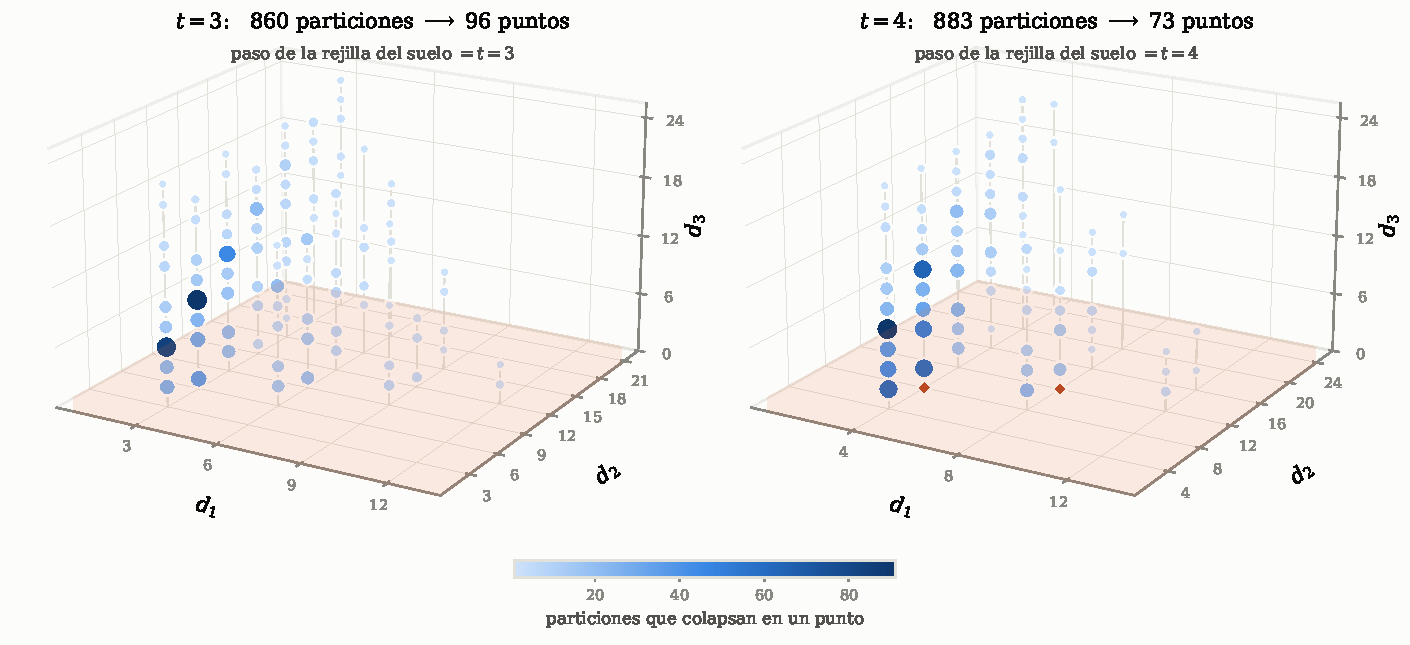
\includegraphics[width=\textwidth]{fig_image_es.pdf}
\caption{La imagen de $\lambda\mapsto(d_1,d_2,d_3)$ sobre todas las $\lambda$ con $|\lambda|\le20$ y
a lo sumo $t+2$ filas, para $t=3$ (izquierda) y $t=4$ (derecha), tomada \emph{salvo el intercambio de
$d_1$ y $d_2$}, bajo el cual \eqref{eq:main} es simétrica; sin esa identificación, y con $A$ y $B$ en
el orden $r_A\le r_B$ del Teorema \ref{thm:main}, los dos paneles llevan $126$ y $92$ puntos en vez
de $96$ y $73$. La compresión es el asunto de la figura: $860$
particiones aterrizan sobre $96$ ternas a la izquierda y $883$ sobre $73$ a la derecha, y el color y
el área dan el número de particiones que va a parar a cada una. El paso de la rejilla del suelo es $t$, pues
$d_1,d_2\in t\ZZ$ por la Proposición \ref{prop:quotient}; el plano sombreado $d_3=0$ es el lugar
concéntrico del Corolario \ref{cor:zero}, donde $s_\lambda$ se anula, así que esas formas no están
en la imagen y se dibujan sobre el plano como rombos. Los dos paneles son las dos paridades, que es
el contenido de la Proposición \ref{rem:lattice}: el impar no lleva ningún rombo, y no puede
llevarlo; el par lleva dos, que son entre ambos la imagen de $32$ particiones.}
\label{fig:image}
\end{figure}

La Figura \ref{fig:image} es una mitad de la imagen: muestra qué ternas se dan, no qué esconde una
terna. La Figura \ref{fig:fibres} es la otra mitad. Sobre cada celda del suelo $(d_1,d_2)$ se levanta
la columna de los tamaños $|\lambda|$ que aterrizan ahí, de modo que una columna es un conjunto de
particiones de tamaños distintos sobre las que $\Phi_t$ toma un único y mismo valor ---y las columnas
no se adelgazan al crecer $|\lambda|$, porque los valores están confinados a un retículo y las
particiones no. La más visible es la fibra de la partición vacía: en $t=3$ el invariante
$I_3=(3,3,2,+1)$ lo comparten $26$ particiones, de $19$ tamaños distintos entre $0$ y $20$, así que
$\Phi_3$ no distingue $\varnothing$ de una forma de veinte cajas.

\begin{figure}[!ht]
\centering
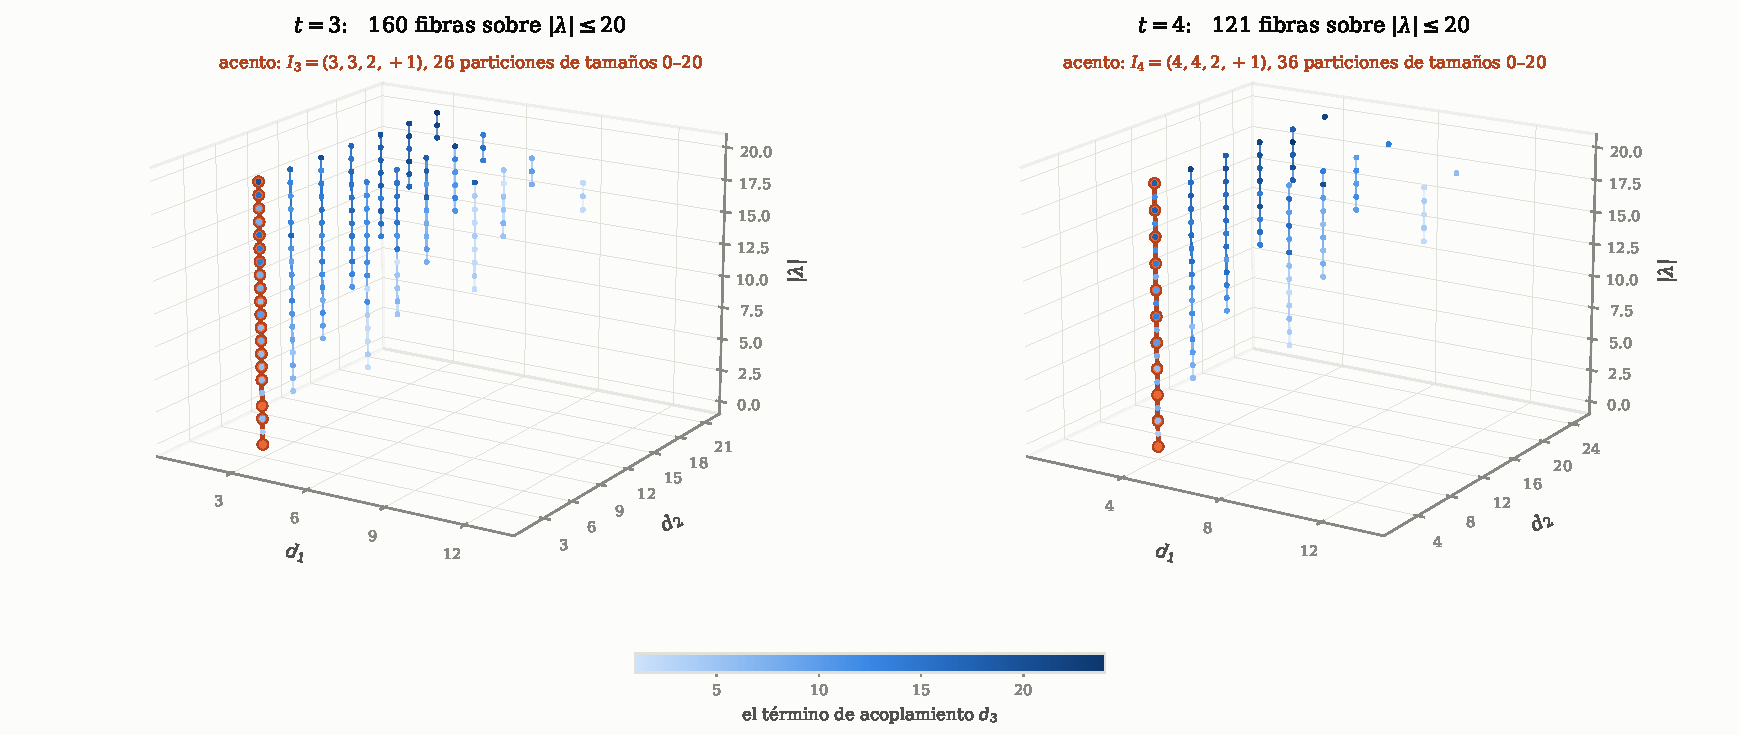
\includegraphics[width=\textwidth]{fig_fibres_es.pdf}
\caption{Las fibras del invariante de la evaluación \eqref{eq:invariant}, complemento de la Figura
\ref{fig:image}: el mismo rango $|\lambda|\le20$, con el término de acoplamiento pasado al color y el
tamaño $|\lambda|$ en el eje vertical. Una columna es una fibra, así que su altura es el rango de
tamaños que este alfabeto no sabe separar; las marcas del suelo son el retículo $t\ZZ$ de la
Proposición \ref{prop:quotient}, y solo está ocupada la mitad $d_1\le d_2$ porque la terna se toma
salvo el intercambio, como en la Figura \ref{fig:image}. Que todas las marcas de una columna lleven
el mismo valor está computado, no supuesto: sobre las $860$ particiones de la izquierda y las $883$
de la derecha el bialternante es constante en cada fibra hasta $10^{-37}$. La columna en color de
acento es la fibra de $\lambda=\varnothing$.}
\label{fig:fibres}
\end{figure}

La Figura 
\ref{fig:fibres} precisa una cosa sobre \eqref{eq:invariant}: $I_t$ es completo pero no mínimo.
El numerador de \eqref{eq:main} es simétrico en $d_1,d_2,d_3$, de modo que el valor solo ve el multiconjunto
$\{d_1,d_2,d_3\}$ junto con el signo, y esa es una reducción real ---sobre $t=4$ y $|\lambda|\le20$
los $121$ invariantes toman solo $110$ valores, mientras que en $t=3$ y el mismo rango los dos
recuentos coinciden. Esa reducción es toda la que hay: por debajo del multiconjunto y del signo no se
pierde nada, y es aquí donde la compresión anunciada en la introducción se vuelve un enunciado exacto
en vez de una cota superior.

\begin{proposition}[el multiconjunto y el signo son exactamente lo que se ve]\label{prop:minimal}
Fíjese $t\ge2$ y sean $\lambda,\mu\in\PP_N$ con $\Phi_t(\lambda;z)\not\equiv0$. Entonces
\[
\Phi_t(\lambda;z)=\Phi_t(\mu;z)
\quad\Longleftrightarrow\quad
\{d_1,d_2,d_3\}(\lambda)=\{d_1,d_2,d_3\}(\mu)\ \text{como multiconjuntos y}\
\varepsilon_\lambda=\varepsilon_\mu .
\]
\end{proposition}

\begin{proof}
$(\Leftarrow)$ es \eqref{eq:main}, cuyo miembro derecho es simétrico en los tres argumentos. Para
$(\Rightarrow)$, obsérvese primero que $\Phi_t(\mu;z)=\Phi_t(\lambda;z)\not\equiv0$, luego $\mu$
tiene también perfil no degenerado y $\tilde d_3(\mu)\ne0$, y los dos invariantes están definidos.
Escribamos $d=d(\lambda)$ y $e=d(\mu)$, con las seis entradas $\ge1$, y pongamos $u=z^{1/2}$, de modo
que $2\sinh(v\theta/2)=u^{v}-u^{-v}$ con exponentes enteros. El denominador de \eqref{eq:main}
depende sólo de $t$, así que la hipótesis es
\[
\varepsilon_\lambda\prod_{i=1}^{3}\bigl(u^{d_i}-u^{-d_i}\bigr)
=\varepsilon_\mu\prod_{i=1}^{3}\bigl(u^{e_i}-u^{-e_i}\bigr).
\]
Usando $u^{v}-u^{-v}=u^{-v}(u^{2v}-1)$ en cada factor y poniendo $D=\sum_id_i$, $E=\sum_ie_i$,
\[
\varepsilon_\lambda\,u^{-D}\prod_{i}\bigl(u^{2d_i}-1\bigr)
=\varepsilon_\mu\,u^{-E}\prod_{i}\bigl(u^{2e_i}-1\bigr).
\]
Cada producto es un polinomio de término constante $(-1)^3=-1$, así que el exponente más bajo que
aparece es $-D$ a la izquierda y $-E$ a la derecha, con coeficientes $-\varepsilon_\lambda$ y
$-\varepsilon_\mu$: luego $D=E$ y $\varepsilon_\lambda=\varepsilon_\mu$, y los dos productos
coinciden. Ahora bien, $u^{2v}-1=\prod_{m\mid2v}Q_m(u)$, donde $Q_m$ es el $m$-ésimo polinomio
ciclotómico --- escrito $Q$ y no $\Phi$, que en este artículo es el objeto. Los $Q_m$ son
irreducibles y distintos dos a dos, así que por factorización única en $\ZZ[u]$ los dos miembros
llevan el mismo multiconjunto de factores ciclotómicos,
\[
\biguplus_i\{m:m\mid 2d_i\}=\biguplus_i\{m:m\mid 2e_i\} .
\]
Su mayor elemento es $\max_i2d_i$ a la izquierda y $\max_i2e_i$ a la derecha, luego coinciden;
borrando de cada lado una copia del conjunto de divisores de ese máximo, y repitiendo dos veces más,
sale $\{2d_1,2d_2,2d_3\}=\{2e_1,2e_2,2e_3\}$.
\end{proof}

\noindent El par (multiconjunto, signo) es entonces un invariante \emph{completo y separador} para
esta evaluación fuera del lugar de anulación --- completo porque el valor factoriza a través de él,
separador porque datos distintos dan valores distintos ---, y eso es un teorema y no un rango. Nos
quedamos a las puertas de llamarlo \emph{mínimo} sin más, porque la minimalidad es relativa a una
clase de invariantes que habría que fijar antes. La hipótesis $\Phi_t(\lambda;z)\not\equiv0$ no es
eliminable y no es un defecto: sobre el lugar de anulación todo invariante colapsa a un único valor,
que es la razón de que \eqref{eq:invariant} mande todo ese lugar a $0$. Mantenemos allí la forma
ordenada porque $d_3$ es la coordenada que aporta el par recíproco y las otras dos no, y el Corolario
\ref{cor:fibregf} describe las fibras de cualquiera de los dos, ya que difieren por una simetría del
numerador y no por nada que el retículo vea.

\begin{proposition}[una forma más corta del signo]\label{rem:sign}
Sea el perfil de residuos no degenerado y $\tilde d_3\ne0$, y ordénense las dos clases
distinguidas de modo que $r_A\le r_B$. Entonces
\begin{equation}\label{eq:shortsign}
\boxed{\;\;\varepsilon_\lambda\;=\;(-1)^{\lfloor t/2\rfloor}\,\sgn(\sigma)\,(-1)^{\,r_A+r_B}\,
\sgn(\tilde d_3)\;\;}
\end{equation}
donde $\sigma$ es la permutación de la \S\ref{sec:background}.
\end{proposition}

\begin{proof}
Sea $w$ la palabra de residuos de $\beta(\lambda)$ leída en orden creciente de columna. Como $\beta$
decrece con el índice de columna, agrupar las partes por clase con los valores decreciendo dentro de
cada clase es la ordenación estable de $w$, luego $\sgn(\sigma)=(-1)^{\inv(w)}$. Ambos miembros de
\eqref{eq:shortsign} llevan el factor $\sgn(\tilde d_3)$, y $\sgn(a_1-b_1)=(-1)^{[a_1<b_1]}$,
de modo que por \eqref{eq:sign} la afirmación equivale a
\begin{equation}\label{eq:signparity}
j_{A_1}+j_{B_1}+\inv(w)+\inv(b_S)+[a_1<b_1]\;\equiv\;
\Bigl\lfloor\tfrac t2\Bigr\rfloor+t+\binom{N+1}{2}+r_A+r_B \pmod 2 .
\end{equation}

Usamos un único conteo de paridad. Sea $u$ una palabra, $p$ una posición, $c=u_p$, y sea $I(p)$ el
número de inversiones de $u$ en las que participa $p$; escribamos $\nu_{<c}$ para el número de letras
de $u$ estrictamente menores que $c$ y $e_p$ para el número de apariciones de $c$ estrictamente antes
de $p$. Poniendo $x=\#\{j<p:u_j>c\}$, las posiciones anteriores a $p$ se reparten como
$p-1=x+e_p+\#\{j<p:u_j<c\}$ y las letras menores que $c$ como
$\nu_{<c}=\#\{j<p:u_j<c\}+\#\{j>p:u_j<c\}$, de donde
\begin{equation}\label{eq:parity}
I(p)\;=\;x+\#\{j>p:u_j<c\}\;=\;2x+e_p+\nu_{<c}-(p-1)\;\equiv\;(p-1)+\nu_{<c}+e_p \pmod 2 .
\end{equation}
Como $b_S$ es $w$ con las letras de las posiciones $j_{A_1}$ y $j_{B_1}$ borradas,
\[
\inv(w)-\inv(b_S)=I(j_{A_1})+I(j_{B_1})
-\bigl[\,\{j_{A_1},j_{B_1}\}\ \text{es una inversión de }w\,\bigr],
\]
y $\inv(w)+\inv(b_S)\equiv\inv(w)-\inv(b_S)$, así que \eqref{eq:parity} calcula el miembro izquierdo
de \eqref{eq:signparity}.

En el perfil de dos clases $r_A<r_B$, y $w$ lleva $r_A$ dos veces, $r_B$ dos veces y cada uno de los
demás residuos una vez. Como $\beta$ decrece con el índice de columna, $a_1>a_2$ sitúa $j_{A_1}$ en
la \emph{primera} aparición de $r_A$, luego allí $e=0$, y lo mismo en $j_{B_1}$. Las letras menores
que $r_A$ son una copia de cada uno de $0,\dots,r_A-1$, luego $\nu_{<r_A}=r_A$; las menores que $r_B$
son esas mismas junto con la segunda copia de $r_A$, luego $\nu_{<r_B}=r_B+1$. Las dos posiciones
forman una inversión exactamente cuando la letra mayor va primero, es decir cuando
$j_{B_1}<j_{A_1}$, es decir cuando $a_1<b_1$. Por tanto
\begin{multline*}
\inv(w)-\inv(b_S)\;\equiv\;(j_{A_1}-1+r_A)+(j_{B_1}-1+r_B+1)+[a_1<b_1]\\
\equiv\;j_{A_1}+j_{B_1}+r_A+r_B+1+[a_1<b_1],
\end{multline*}
y al sustituir esto en \eqref{eq:signparity} las columnas y $[a_1<b_1]$ se cancelan por pares y queda
$\lfloor t/2\rfloor+t+\binom{N+1}{2}\equiv1$.

En el perfil de tamaño tres $r_A=r_B=:r$ y la clase $\{p>q>p'\}$ ocupa las columnas $j_1<j_2<j_3$ con
$A=\{p,q\}$ y $B=\{q,p'\}$, de modo que $j_{A_1}=j_1$ y $j_{B_1}=j_2$ llevan la misma letra $r$, con
$e=0$ y $e=1$ respectivamente y $\nu_{<r}=r$ en ambos; dos letras iguales no forman inversión, y
$a_1>b_1$. Luego $\inv(w)-\inv(b_S)\equiv j_1+j_2+1$, que es de nuevo la expresión anterior porque
$r_A+r_B=2r$ y $[a_1<b_1]=0$, y \eqref{eq:signparity} se reduce a la misma congruencia.

Por último $N=t+2$, así que esa congruencia dice
$\lfloor t/2\rfloor+t+\binom{t+3}{2}\equiv1$: para $t=2m$ sus tres términos son $m$, $0$ y $m+1$, y
para $t=2m+1$ son $m$, $1$ y $m$. Ambas sumas son impares, y la identidad vale para todo $t\ge2$.
\end{proof}

La ordenación por residuo no es una comodidad, y vale la pena decir por qué. Intercambiar los dos
bloques cambia el signo de $\kappa_{11}$, el del Lema \ref{lem:L4} --- por su factor
$\sgn(a_1-b_1)$ --- y también el de
$\sgn(\tilde d_3)$, luego deja invariante a $\varepsilon_\lambda$, que es su producto; como no
puede ser de otro modo, porque $\varepsilon_\lambda$ va unido a $\lambda$. El miembro derecho de
arriba \emph{no} queda invariante: $(-1)^{r_A+r_B}$ es simétrico, así que solo cambia de signo su
último factor. Sin una regla que fije cuál de los bloques es $A$, el miembro derecho no es siquiera
una función de $\lambda$. La hipótesis entra en la demostración en un único punto: es lo que hace
que $\nu_{<r_A}=r_A$ y $\nu_{<r_B}=r_B+1$ y no al revés, y suprimirla intercambia esos dos conteos y
rompe \eqref{eq:signparity}.

Leída al revés, \eqref{eq:shortsign} dice que $\Phi_t$ es función de un dato combinatorio pequeño y
de nada más, y lo dice para todo $t$ y no sobre un rango: por el Teorema \ref{thm:main} el triple
$(d_1,d_2,d_3)$ determina $\Phi_t$ salvo signo, y añadiendo $\sgn(\sigma)$, el par ordenado
$r_A\le r_B$ y la \emph{orientación} $\sgn(\tilde d_3)$ lo determina por completo. La
forma de $\lambda$ no entra en ninguna otra parte. La orientación no es opcional, y esa parte sigue
siendo una comprobación y no una demostración: sobre $t\le6$ y $|\lambda|\le14$, poner
$\sgn(a_1-b_1)$ en su lugar deja colisiones en $t=2$.

%======================================================================
\section{Demostración del Teorema \ref{thm:main}}\label{sec:proof}

La demostración usa el determinante de Vandermonde, el desarrollo de Laplace y un lema de
cancelación. Damos los pasos por separado para que quien contraste los guiones auxiliares pueda
localizar cualquier discrepancia.

\begin{figure}[!ht]
\centering
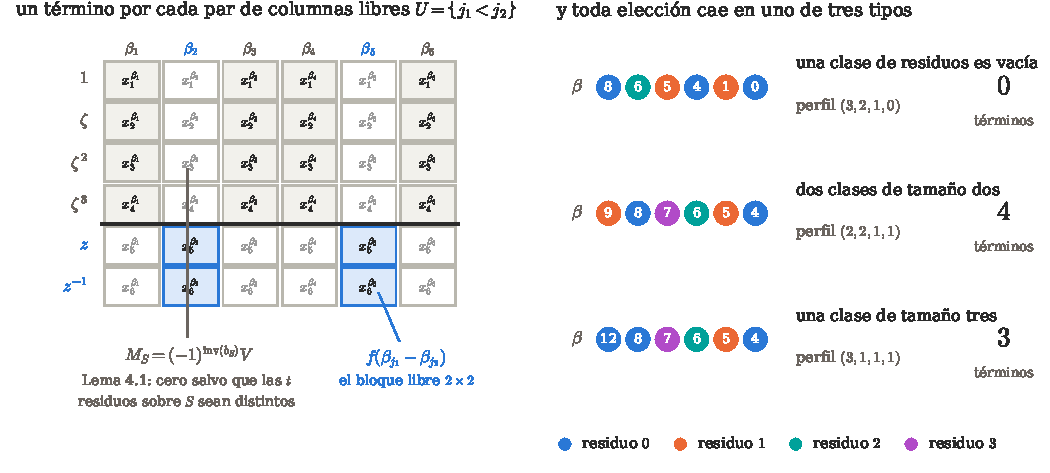
\includegraphics[width=\textwidth]{fig_laplace_es.pdf}
\caption{La arquitectura de la demostración, dibujada con $t=4$, $N=6$. \emph{Izquierda:} el
determinante $\det(x_i^{\beta_j})$ desarrollado por las $t$ filas congeladas. Cada elección de las
dos columnas $U=\{j_1<j_2\}$ que se dejan a las filas libres $z,z^{-1}$ deja un menor $t\times t$
$M_S$ sobre las columnas complementarias, que por el Lema \ref{lem:L1} vale $\pm V$ o cero, por el
bloque $2\times2$ $f(\beta_{j_1}-\beta_{j_2})$. \emph{Derecha:} por el recuento del exceso dos
\eqref{eq:excess} sólo hay tres perfiles de residuos, uno por fila, cada uno sobre un beta-conjunto
que lo realiza; el número de la derecha es cuántas elecciones de $U$ sobreviven, contado y no
afirmado --- $0$, $4$ y $3$, que es la tricotomía sobre la que se organiza la sección. El color es
la clase de residuos. Calculada por \texttt{anc/fig\_proof.py}.}
\label{fig:laplace}
\end{figure}

El desarrollo en sí es el movimiento habitual de esta literatura y no reclamamos nada por él: Albion
\cite{Alb25} aplica el desarrollo de Laplace a un determinante de esta forma \emph{según la
estructura de bloques dada}, manteniendo fijo un primer conjunto de filas, siguiendo a Krattenthaler
y a Ciucu--Krattenthaler. Lo particular aquí no es el desarrollo, sino con qué se topa.

Lo que el argumento hace en realidad es clasificar, no calcular. Desarrollar por las $t$ filas
congeladas deja un término por cada manera de elegir qué dos columnas \emph{no} lo están, y el
recuento del exceso dos dice que toda elección cae en exactamente uno de tres tipos combinatorios:
no sobrevive ninguna (una clase de residuos es vacía), sobreviven cuatro (dos clases de tamaño dos) o
sobreviven tres (una clase de tamaño tres). Todo lo que sigue es contabilidad dentro de un tipo, y el
Lema \ref{lem:L5} muestra que los dos últimos son un mismo enunciado visto dos veces. La Figura \ref{fig:laplace} es esa frase dibujada.

\begin{lemma}\label{lem:L1}
Sea $S$ un conjunto de $t$ columnas y $M_S=\det(\zeta^{k\beta_j})_{0\le k<t,\,j\in S}$. Entonces
$M_S=0$ salvo que los residuos $\{\beta_j\bmod t:j\in S\}$ sean dos a dos distintos, en cuyo caso
$M_S=(-1)^{\inv(b_S)}V$.
\end{lemma}

\begin{proof}
Como $\zeta^{k\beta_j}=(\zeta^{\beta_j})^k$, la matriz es de Vandermonde en los valores
$y_j=\zeta^{\beta_j}$, cuyo determinante es $\prod_{j<j'}(y_{j'}-y_j)$. El valor $y_j$ depende de
$\beta_j$ solo módulo $t$, luego dos columnas de $S$ que compartan residuo anulan el determinante. Si
los residuos son dos a dos distintos, $|S|=t$ obliga a $\{y_j\}_{j\in S}=\zt$ como conjunto, y el
determinante de Vandermonde es alternante en sus argumentos, luego vale $V$ por el signo de la
permutación que ordena $b_S$ crecientemente, que es $(-1)^{\inv(b_S)}$.
\end{proof}

\begin{lemma}\label{lem:L2}
$\det\bigl(x_i^{N-j}\bigr)_{i,j=1}^{N}=(-1)^{\binom t2}\,V\,(z^t-1)(z^{-t}-1)(z-z^{-1})$ para el
alfabeto $x=(1,\zeta,\dots,\zeta^{t-1},z,z^{-1})$ en ese orden.
\end{lemma}

\begin{proof}
El determinante es $\prod_{i<i'}(x_i-x_{i'})$. Los pares dentro de $\zt$ aportan
$\prod_{k<k'}(\zeta^k-\zeta^{k'})=(-1)^{\binom t2}V$; los pares $(\zeta^k,z)$ aportan
$\prod_k(\zeta^k-z)=(-1)^t(z^t-1)$ y los pares $(\zeta^k,z^{-1})$ aportan $(-1)^t(z^{-t}-1)$; el
último par aporta $z-z^{-1}$. Los dos factores $(-1)^t$ se cancelan.
\end{proof}

\noindent Lo calculamos porque son tres líneas, no porque sea desconocido: un determinante sobre un
alfabeto cerrado bajo $x\mapsto x^{-1}$, evaluado en forma de producto cerrado, es exactamente el
asunto del complemento de Krattenthaler al cálculo de determinantes \cite[\S5.11]{KratADCC}, cuyo
Lema 20 lleva entre sus casos particulares las fórmulas del denominador de Weyl para $B_n$, $C_n$ y
$D_n$. Lo que esa literatura no evalúa ---y lo que el lema siguiente necesita--- es ese mismo
determinante con una órbita de raíces de la unidad dentro del alfabeto.

\begin{lemma}\label{lem:L3}
Sea $\mathcal U$ el conjunto de pares $U=\{j_1<j_2\}$ de columnas cuyo complementario $S_U$ lleva las
$t$ clases de residuos. Entonces
\[
\Phi_t(\lambda;z)=\frac{(-1)^{\,t+\binom{N+1}{2}}}{(z^t-1)(z^{-t}-1)(z-z^{-1})}
\sum_{U\in\mathcal U}(-1)^{\,j_1+j_2+\inv(b_{S_U})}\,f(\beta_{j_1}-\beta_{j_2}).
\]
\end{lemma}

\begin{proof}
Desarrollando el numerador por Laplace a lo largo de las primeras $t$ filas,
\[
\det\bigl(x_i^{\beta_j}\bigr)=\sum_{|S|=t}(-1)^{\binom{t+1}{2}+\sum_{j\in S}j}\,M_S\,C_{S^c},
\]
donde para $S^c=\{j_1<j_2\}$ el menor complementario $2\times2$ es
$z^{\beta_{j_1}-\beta_{j_2}}-z^{-(\beta_{j_1}-\beta_{j_2})}=f(\beta_{j_1}-\beta_{j_2})$. Por el Lema
\ref{lem:L1} solo contribuyen los $S$ con residuos dos a dos distintos. Escribiendo
$\sum_{j\in S}j=\binom{N+1}{2}-j_1-j_2$ y dividiendo por el Lema \ref{lem:L2}, los factores $V$ se
cancelan y $(-1)^{\binom{t+1}{2}-\binom{t}{2}}=(-1)^t$.
\end{proof}

Si algún $n_i=0$, ningún $S$ de tamaño $t$ lleva todos los residuos, $\mathcal U=\varnothing$ y
$\Phi_t=0$: es el Teorema \ref{thm:main}(i). En caso contrario todos los $n_i\ge1$ y por
\eqref{eq:excess} o bien dos clases tienen tamaño dos, y entonces $S_U$ debe descartar un elemento de
cada una y $|\mathcal U|=4$, o bien una clase tiene tamaño tres, y entonces $S_U$ descarta dos de los
tres y $|\mathcal U|=3$.

\begin{lemma}[el movimiento de columna]\label{lem:L4}
Sean $A$ y $B$ clases distintas de tamaño dos, en las columnas $j_{A_1}<j_{A_2}$ y
$j_{B_1}<j_{B_2}$. Para $i,j\in\{1,2\}$ sea $U_{ij}$ el par formado por la columna de $a_i$ y la de
$b_j$, y sea $\kappa_{ij}=(-1)^{\,j_{A_i}+j_{B_j}+\inv(b_{S_{U_{ij}}})}\sgn(a_i-b_j)$, de modo que
el término $U_{ij}$ del Lema \ref{lem:L3} vale $\kappa_{ij}f(a_i-b_j)$. Entonces
$\kappa_{ij}=\kappa_{11}(-1)^{i-1}(-1)^{j-1}$.
\end{lemma}

\begin{proof}
Fijemos $j$ y comparemos $i=1$ con $i=2$. Los conjuntos $S_{U_{1j}}$ y $S_{U_{2j}}$ difieren solo en
que el primero contiene la columna $j_{A_2}$ y el segundo la columna $j_{A_1}$, y la letra que llevan
es el residuo $r_A$ en ambos casos. Pasar de una palabra a la otra mueve esa letra a través de
exactamente las columnas conservadas estrictamente entre $j_{A_1}$ y $j_{A_2}$, y ninguna de esas
letras es igual a $r_A$ porque la clase $A$ tiene solo dos elementos; cada cruce cambia la paridad de
$\inv$. Por tanto
\[
(-1)^{\inv(b_{S_{U_{1j}}})-\inv(b_{S_{U_{2j}}})}
=(-1)^{(j_{A_2}-j_{A_1}-1)-[\,a_2<b_j<a_1\,]},
\]
usando que $\beta$ es estrictamente decreciente en el índice de columna, de modo que $j_{B_j}$ está
estrictamente entre $j_{A_1}$ y $j_{A_2}$ exactamente cuando $a_2<b_j<a_1$. Multiplicando por el
factor de Laplace $(-1)^{j_{A_1}+j_{A_2}}$,
\[
\frac{\kappa_{1j}}{\kappa_{2j}}
=(-1)^{2j_{A_2}-1}(-1)^{[\,a_2<b_j<a_1\,]}\sgn(a_1-b_j)\sgn(a_2-b_j)=-1,
\]
porque $\sgn(a_1-b_j)\sgn(a_2-b_j)=-1$ exactamente cuando $b_j$ está entre $a_2$ y $a_1$.
Intercambiando los papeles de $A$ y $B$ se obtiene $\kappa_{i1}/\kappa_{i2}=-1$.
\end{proof}

\begin{lemma}\label{lem:L5}
Para todos $c,p,q$ y todos $u,v$,
\begin{align*}
\text{\rm(a)}&\quad \sum_{\epsilon,\eta\in\{\pm1\}}\epsilon\eta\,f(c+\epsilon p+\eta q)=f(c)f(p)f(q),\\
\text{\rm(b)}&\quad f(2u)-f(2u+2v)+f(2v)=-f(u)f(v)f(u+v).
\end{align*}
\end{lemma}

\begin{proof}
Para (a), $\sum_{\epsilon,\eta}\epsilon\eta\,z^{c+\epsilon p+\eta q}
=z^{c}\bigl(\sum_\epsilon\epsilon z^{\epsilon p}\bigr)\bigl(\sum_\eta\eta z^{\eta q}\bigr)
=z^{c}f(p)f(q)$, y el mismo cálculo para los exponentes negativos da $z^{-c}(-f(p))(-f(q))$;
réstese. Para (b), pónganse $s=z^u$, $w=z^v$ y desarróllese
$(s-s^{-1})(w-w^{-1})(sw-s^{-1}w^{-1})$: los ocho términos se recombinan como
$(s^2w^2-s^{-2}w^{-2})-(s^2-s^{-2})-(w^2-w^{-2})=f(2u+2v)-f(2u)-f(2v)$.
\end{proof}

\begin{proof}[Demostración del Teorema \ref{thm:main}]
En el perfil de dos clases, los Lemas \ref{lem:L3} y \ref{lem:L4} dan
\[
\sum_{U\in\mathcal U}(\cdots)=\kappa_{11}\sum_{i,j}(-1)^{i-1}(-1)^{j-1}f(a_i-b_j).
\]
Escribiendo $a_i=\alpha+\epsilon_ip$ y $b_j=\gamma+\eta_jq$ con $p=d_1/2$, $q=d_2/2$ y
$\epsilon=\eta=(+1,-1)$, se tiene $a_i-b_j=c+\epsilon_ip-\eta_jq$ con $c=\alpha-\gamma$. Sustituyendo
$\eta$ por $-\eta$, la suma se convierte en
$-\sum_{\epsilon,\eta}\epsilon\eta f(c+\epsilon p+\eta q)$, que vale $-f(c)f(p)f(q)$ por el Lema
\ref{lem:L5}(a). Como $(z^t-1)(z^{-t}-1)=2-z^t-z^{-t}=-f(t/2)^2$ y $z-z^{-1}=f(1)$, los dos signos
menos se cancelan, y sustituyendo $f(u)=2\sinh(u\theta)$ los factores numéricos se cancelan. Aquí
$2c=\tilde d_3$. Si $\tilde d_3=0$, entonces $f(c)=0$ y la suma entera se anula, que es la primera
afirmación de {\rm(ii)}; en caso contrario
$\sinh(c\theta)=\sgn(\tilde d_3)\sinh(d_3\theta/2)$, lo que da \eqref{eq:main} con
$\varepsilon_\lambda=(-1)^{\,t+\binom{N+1}{2}}\kappa_{11}\sgn(\tilde d_3)$, que es
\eqref{eq:sign} por la definición de $\kappa_{11}$ en el Lema \ref{lem:L4}.

Para el perfil de tamaño tres $\{p>q>r\}$ en las columnas $j_1<j_2<j_3$ se aplica el mismo argumento
de movimiento de columna, de nuevo porque ninguna letra estrictamente entre dos de esas columnas
lleva el residuo de la clase, y da signos alternantes $(\varsigma,-\varsigma,\varsigma)$ para los
tres términos $f(p-q)$, $f(p-r)$, $f(q-r)$. Por el Lema \ref{lem:L5}(b) con $u=(p-q)/2$,
$v=(q-r)/2$ la suma es $-\varsigma f(u)f(v)f(u+v)$, que es la fórmula de dos clases para $A=\{p,q\}$,
$B=\{q,r\}$ con $\varsigma=\kappa_{11}$. Equivalentemente, la cuarta selección ausente del perfil de
dos clases descartaría $q$ dos veces y su término lleva $f(0)=0$, de modo que los dos perfiles son un
solo enunciado.
\end{proof}

Todos los enunciados de este artículo se comprobaron además numéricamente; los recuentos se recogen
una sola vez, en la \S\ref{sec:verif}, en lugar de repetirse según van surgiendo.

%======================================================================
\section{Independencia en el lugar recíproco}\label{sec:independence}

El Teorema 5.3 de \cite{AK25} está enunciado para variables libres, y $(z,\zb)$ no es un par libre.
Nada de esta sección lo contradice: el lugar recíproco queda fuera de sus hipótesis, no en contra de
ellas, y lo que hacemos aquí es determinar en qué se convierte allí su criterio. Leída al pie de la
letra, \eqref{eq:AK53} diría que para $\ell(\lambda)\le2$ se tiene
$s_\lambda(z,\zb,\zt)=s_\lambda(z,\zb)$ exactamente sobre los $t$-núcleos. El Teorema
\ref{thm:main} evalúa el miembro izquierdo para toda $\lambda$, y al comparar ambos se ve que el
lugar recíproco lleva más soluciones: exactamente una familia. Medir cuánto sobrevive un criterio a
una degeneración es una manera de decir lo afilado que era, y la respuesta aquí es que lo es salvo
una sola familia.

Aislamos primero cuándo $\Phi_t$ degenera en un solo carácter.

\begin{lemma}\label{lem:single}
$\Phi_t(\lambda;z)=\pm\chi_k(z)$ para algún $k\ge0$ si y solo si el multiconjunto $\{d_1,d_2,d_3\}$
contiene $t$ al menos dos veces, y en tal caso la entrada restante vale $2(k+1)$.
\end{lemma}

\begin{proof}
Pongamos $u=z^{1/2}$, de modo que $2\sinh(d_i\theta/2)=u^{d_i}-u^{-d_i}$,
$2\sinh(t\theta/2)=u^{t}-u^{-t}$ y $2\sinh\theta=u^{2}-u^{-2}$; todos los exponentes son enteros. Por
\eqref{eq:main}, la igualdad afirmada es
\[
\prod_{i=1}^{3}\bigl(u^{d_i}-u^{-d_i}\bigr)
=\pm\bigl(u^{t}-u^{-t}\bigr)^{2}\bigl(u^{2k+2}-u^{-2k-2}\bigr).
\]
Usando $u^{n}-u^{-n}=u^{-n}(u^{2n}-1)$ en cada factor y comparando los prefactores monomiales se
obtiene $d_1+d_2+d_3=2t+2(k+1)$ junto con
\[
\prod_{i=1}^{3}\bigl(u^{2d_i}-1\bigr)=\pm\bigl(u^{2t}-1\bigr)^{2}\bigl(u^{4(k+1)}-1\bigr),
\]
y evaluando en $u=0$ el signo queda fijado en $+$. Ahora $u^{2n}-1=\prod_{m\mid 2n}Q_m(u)$ con
$Q_m$ los polinomios ciclotómicos como en la Proposición \ref{prop:minimal}, que son irreducibles y
distintos dos a dos, de modo que por
factorización única en $\ZZ[u]$ ambos miembros tienen el mismo multiconjunto de factores
ciclotómicos. A la izquierda ese multiconjunto es $\biguplus_i\{m:m\mid 2d_i\}$ y a la derecha
$2\times\{m:m\mid 2t\}\uplus\{m:m\mid 4(k+1)\}$. Su mayor elemento es $\max_i 2d_i$ a la izquierda y
$\max(2t,4(k+1))$ a la derecha; borrando de ambos lados el conjunto de divisores de ese máximo y
repitiendo dos veces más se llega a
\[
\{2d_1,2d_2,2d_3\}=\{2t,\,2t,\,4(k+1)\}
\]
como multiconjuntos, que es lo afirmado. El recíproco es el mismo cálculo leído al revés.
\end{proof}

\begin{theorem}\label{thm:extra}
Sea $\ell(\lambda)\le2$. Entonces
\[
\Phi_t(\lambda;z)=s_\lambda(z,\zb)
\]
---una igualdad, y no una igualdad salvo signo--- si y solo si o bien
$\lambda=\core_t(\lambda)$, o bien
\begin{equation}\label{eq:extra}
t\ \text{es par}\quad\text{y}\quad \lambda=\Bigl(\lambda_2+\tfrac{3t}{2}-1,\ \lambda_2\Bigr)
\quad\text{con}\quad \tfrac t2\le\lambda_2\le t-1 .
\end{equation}
En el segundo caso $\{d_1,d_2,d_3\}=\{3t,t,t\}$ y $\varepsilon_\lambda=+1$, mientras que
$\core_t(\lambda)=\bigl(\tfrac t2-1+j,j\bigr)$ y $\quot_t(\lambda)$ tiene como única componente no
vacía $(2)$, en la posición $j=\lambda_2-\tfrac t2$.
\end{theorem}

La Figura \ref{fig:locus} es el enunciado computado en vez de afirmado: ambas familias están
dibujadas sobre un rango de $t$, y el $t$ impar donde \eqref{eq:extra} no puede darse es el control.

\begin{figure}[!ht]
\centering
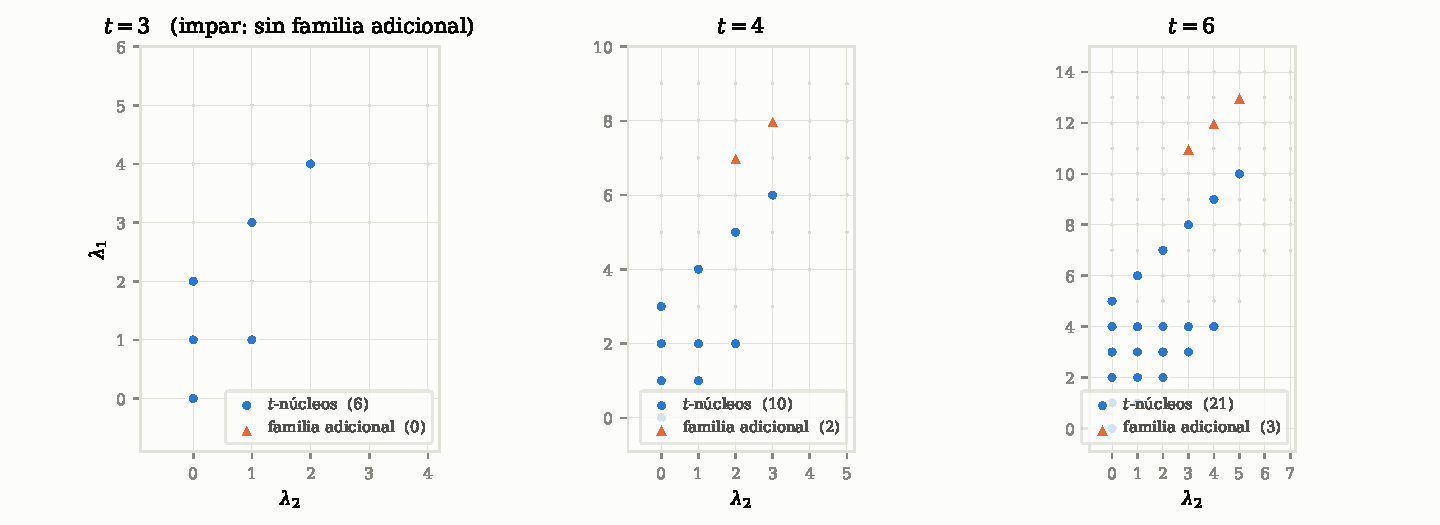
\includegraphics[width=\textwidth]{fig_locus_es.pdf}
\caption{El Teorema \ref{thm:extra}, calculado y no afirmado. Para toda $\lambda$ de dos filas en
rango se evaluaron ambos miembros de $\Phi_t(\lambda;z)=\pm s_\lambda(z,\zb)$; se representan las
particiones donde coinciden, coloreadas por familia. Los círculos son los $t$-núcleos, las soluciones
ya descritas por \eqref{eq:AK53}; los triángulos son la familia adicional \eqref{eq:extra}, que crea
la especialización recíproca. El caso impar $t=3$ es el control: por el Teorema \ref{thm:extra} allí
no puede existir solución adicional, y no se halla ninguna.}
\label{fig:locus}
\end{figure}

\begin{proof}
Como $\ell(\lambda)\le 2$ y $N=t+2$, el conjunto beta es
$\beta(\lambda)=\bigl(A'+t,\;B'+t,\;t-1,t-2,\dots,1,0\bigr)$ donde
\[
A':=\lambda_1+1,\qquad B':=\lambda_2,\qquad A'>B'\ge0 .
\]
El bloque $\{0,1,\dots,t-1\}$ toca cada clase de residuos exactamente una vez, luego ninguna clase es
vacía y las dos partes grandes deciden el perfil. Escribamos $A'=t\alpha+\rho_A$ y
$B'=t\gamma+\rho_B$ con $0\le\rho_A,\rho_B\le t-1$. Como $s_\lambda(z,\zb)=\chi_{\lambda_1-\lambda_2}(z)$,
el Lema \ref{lem:single} dice que la afirmación se cumple exactamente cuando $\{d_1,d_2,d_3\}$
contiene $t$ dos veces y la tercera entrada es $2(\lambda_1-\lambda_2+1)=2(A'-B')$.

\emph{Caso $\rho_A=\rho_B=:\rho$.} Una clase tiene tamaño tres, a saber $\{A'+t,B'+t,\rho\}$, y por el
Teorema \ref{thm:main} los tres argumentos son $d_1=A'-B'$, $d_2=B'+t-\rho=t(\gamma+1)$,
$d_3=A'+t-\rho=t(\alpha+1)$. Aquí $t\mid A'-B'$, digamos $A'-B'=ts$ con $s\ge1$. El par $d_2=d_3=t$
fuerza $\alpha=\gamma=0$, luego $A'=B'$, excluido. El par $d_1=d_3=t$ fuerza $s=1$ y $\alpha=0$,
luego $A'<t$ y $A'=B'+t\ge t$, excluido. El par $d_1=d_2=t$ fuerza $s=1$ y $\gamma=0$, es decir
$A'=B'+t$ con $B'<t$; entonces $\alpha=1$ y la tercera entrada es $d_3=2t=2(A'-B')$, como se
requiere. Este caso aporta pues exactamente las $\lambda$ con $A'=B'+t$, $B'<t$.

\emph{Caso $\rho_A\ne\rho_B$.} Dos clases tienen tamaño dos, a saber $\{A'+t,\rho_A\}$ y
$\{B'+t,\rho_B\}$, y los tres argumentos son
\[
d_A=t(\alpha+1),\qquad d_B=t(\gamma+1),\qquad
d_3=\bigl|\,t(\alpha-\gamma)+2(\rho_A-\rho_B)\,\bigr| .
\]
Si $d_A=d_B=t$ entonces $\alpha=\gamma=0$, luego $A',B'<t$ y $d_3=2|\rho_A-\rho_B|=2(A'-B')$
automáticamente: toda tal $\lambda$ es solución. En otro caso exactamente uno de $d_A,d_B$ vale $t$ y
$d_3=t$. Si $\alpha=0$ y $\gamma\ge1$, entonces $|-t\gamma+2(\rho_A-\rho_B)|=t$ con
$|\rho_A-\rho_B|\le t-1$ fuerza $\gamma=2$ y $\rho_A-\rho_B=t/2$; pero entonces
$\lambda_1=A'-1=\rho_A-1<t$ mientras que $\lambda_2=B'\ge2t$, en contra de $\lambda_1\ge\lambda_2$.
Si $\gamma=0$ y $\alpha\ge1$, entonces $|t\alpha+2(\rho_A-\rho_B)|=t$ fuerza, para $\alpha=1$,
$\rho_A=\rho_B$ (excluido), y para $\alpha=2$,
\[
\rho_B-\rho_A=\tfrac t2,
\]
lo que exige $t$ par; $\alpha\ge3$ da $|2(\rho_A-\rho_B)|\ge2t$, imposible. Luego $A'=2t+\rho_A$,
$B'=\rho_B=\rho_A+\tfrac t2$, de donde
\[
\lambda_1=2t+\rho_A-1,\qquad \lambda_2=\rho_A+\tfrac t2,\qquad
\lambda_1-\lambda_2=\tfrac{3t}{2}-1,
\]
y $\rho_B\le t-1$ da $0\le\rho_A\le\tfrac t2-1$, es decir $\tfrac t2\le\lambda_2\le t-1$. La entrada
restante es $d_A=t(\alpha+1)=3t=2(\lambda_1-\lambda_2+1)$, como se requiere. Esto es
\eqref{eq:extra}.

Queda identificar las soluciones del primer caso de cada análisis con los $t$-núcleos. Para
$\ell(\lambda)\le2$ el conjunto beta en dos posiciones es $(A',B')$, y $\lambda$ es un $t$-núcleo si
y solo si ningún número beta puede rebajarse en $t$ hasta una posición no negativa desocupada, es
decir si y solo si $B'<t$ y o bien $A'<t$ o bien $A'=B'+t$. Son exactamente las dos familias
halladas. Por último, en el caso \eqref{eq:extra} la clase $\rho_A$ lleva $\{2t+\rho_A+t,\rho_A\}$,
luego su componente del cociente es $(2)$, toda otra componente es vacía, y el núcleo es el
enunciado.

\emph{El signo.} Las dos familias lo consiguen por razones distintas. Sobre los $t$-núcleos la
igualdad es \eqref{eq:AK53} misma, que es una igualdad y no una igualdad salvo signo, así que no hay
nada que probar. Sobre \eqref{eq:extra}, escríbase $t=2m$ y $\lambda_2=m+j$ con $0\le j\le m-1$, de
modo que $\rho_A=j$ y $\rho_B=m+j$ y
\[
\beta(\lambda)=\bigl(6m+j,\;3m+j,\;2m-1,2m-2,\dots,1,0\bigr).
\]
Reduciendo módulo $t=2m$, la palabra de residuos leída en orden creciente de columna es
\[
w=\bigl(j,\;m+j,\;2m-1,2m-2,\dots,1,0\bigr),
\]
puesto que $6m+j\equiv j$ y $3m+j\equiv m+j$, esto último porque $j\le m-1$. Sus inversiones son de
tres clases: la cola decreciente aporta $\binom{2m}{2}$; la primera letra está por encima de
exactamente las $j$ letras de la cola $0,\dots,j-1$; la segunda, por encima de exactamente las $m+j$
letras $0,\dots,m+j-1$; y las dos primeras letras están en orden creciente, así que no aportan
ninguna. Por tanto
\begin{equation}\label{eq:extrainv}
\inv(w)=\binom{2m}{2}+j+(m+j)=2m^{2}+2j\;\equiv\;0\pmod2 ,
\end{equation}
luego $\sgn(\sigma)=(-1)^{\inv(w)}=+1$ por la primera línea de la prueba de la Proposición
\ref{rem:sign}. Las dos clases distinguidas son $r_A=j<r_B=m+j$, que llevan $A=\{6m+j,\,j\}$ y
$B=\{3m+j,\,m+j\}$, de modo que $\tilde d_3=(6m+2j)-(4m+2j)=2m>0$ y $\sgn(\tilde d_3)=+1$. Los dos
factores restantes de \eqref{eq:shortsign} son $(-1)^{\lfloor t/2\rfloor}=(-1)^{m}$ y
$(-1)^{r_A+r_B}=(-1)^{m+2j}=(-1)^{m}$, cuyo producto es $+1$. Así pues $\varepsilon_\lambda=+1$, y
como $d_1=6m=3t$, $d_2=2m=t$ y $d_3=2m=t$, \eqref{eq:main} dice
\[
\Phi_t(\lambda;z)=\frac{\sinh(3t\theta/2)\sinh^{2}(t\theta/2)}{\sinh^{2}(t\theta/2)\sinh\theta}
=\chi_{\frac{3t}{2}-1}(z)=\chi_{\lambda_1-\lambda_2}(z)=s_\lambda(z,\zb),
\]
sin ningún signo que arrastrar.
\end{proof}

\noindent Lo que compra \eqref{eq:extrainv} no es decoración. Enunciado salvo signo, el Teorema
\ref{thm:extra} dice que la especialización crea una familia de formas sobre las que el twist es
invisible \emph{salvo un signo}, que es un enunciado más débil que el que \eqref{eq:AK53} hace sobre
los núcleos; con el signo resuelto, las dos familias son soluciones de la misma ecuación, y ``el
lugar recíproco adquiere exactamente una familia más'' es literalmente cierto.

\begin{remark}\label{rem:why}
El Lema \ref{lem:single} controla el valor sólo salvo signo, y por eso el signo del Teorema
\ref{thm:extra} necesita el párrafo aparte de arriba en lugar de salir de la clasificación.

La familia adicional pertenece a la especialización y no al alfabeto. El paso es el
\cite[Lema 5.2]{AK25}, sobre el que se apoya el \cite[Teorema 5.3]{AK25}: reduce la independencia a
la anulación de $s_{\lambda/\mu}$ en el alfabeto torcido para todo $\mu\subsetneq\lambda$, y la
reducción usa la independencia lineal de los caracteres universales $f_\mu$ en las variables libres. En el lugar recíproco
$s_\mu(z,\zb)=\chi_{\mu_1-\mu_2}(z)$ depende solo de $\mu_1-\mu_2$, luego $s_{(1)}$, $s_{(2,1)}$ y
$s_{(3,2)}$ coinciden allí y esa independencia deja de estar disponible; el Teorema \ref{thm:extra}
mide la diferencia. Un control confirma la lectura: para $\lambda=(3,1)$ y $t=2$ se tiene
$s_\lambda(\zt,z,\zb)=s_\lambda(z,\zb)$, mientras que $s_\lambda(\zt,x,y)\ne s_\lambda(x,y)$ para
$x,y$ libres.
\end{remark}

Así pues, el criterio no sobrevive intacto a la especialización, y lo que adquiere es pequeño y
nombrable: una familia, para formas de dos filas, indexada por un elemento de orden dos del retículo
de residuos y clasificada por su núcleo y su cociente. Las soluciones adicionales pertenecen al lugar
recíproco y no al alfabeto ---existen porque una especialización ha retirado una independencia lineal
que el argumento original usaba, y ese paso que falta es exactamente lo que mide el Teorema
\ref{thm:extra}.

%======================================================================
\section{Una enumeración en la que sobrevive un parámetro}\label{sec:enum}

Desarrollando $s_\lambda$ sobre tablas semiestándar, el Teorema \ref{thm:main} se convierte en una
fórmula de producto para un recuento pesado. Sea $m_k(T)$ el número de entradas iguales a $k$ en $T$.

\begin{corollary}\label{cor:enum}
Desarrollando $s_\lambda$ sobre tablas semiestándar y aplicando el Teorema \ref{thm:main}: para todo
$t\ge2$ y toda $\lambda\in\PP_{t+2}$,
\[
\sum_{T\in\mathrm{SSYT}(\lambda,\,t+2)}
\zeta^{\,\sum_{k=1}^{t}(k-1)m_k(T)}\;z^{\,m_{t+1}(T)-m_{t+2}(T)}
\;=\;\varepsilon_\lambda\,
\frac{\sinh(d_1\theta/2)\sinh(d_2\theta/2)\sinh(d_3\theta/2)}{\sinh^2(t\theta/2)\sinh\theta}.
\]
\end{corollary}

Para $t=2$ el peso es $(-1)^{m_2(T)}$, y si $\lambda=(c^{\,a})$ es rectangular entonces
$\mathrm{SSYT}(\lambda,4)$ está en biyección con las particiones planas en una caja
$a\times(4-a)\times c$, equivalentemente con las teselaciones de rombos de un hexágono. El Corolario
\ref{cor:enum} es entonces una $(-1)$-enumeración de esos objetos \emph{refinada por un parámetro
libre} $z$, que registra la diferencia entre los números de entradas $3$ y $4$. Poniendo $z=1$ se
recupera el recuento con signo puro, que por \eqref{eq:main} vale $\pm d_1d_2d_3/(2t^2)$: para la
$a=2$, $c=2$ vale $4$; para $a=2$, $c=4$ vale $9$; para $a=3$, $c=3$ vale $-6$.

\begin{example}\label{ex:boxes}
Tomando $\lambda=(c^{\,a})$ con $1\le a\le4$ y $t=2$, la forma tiene a lo sumo cuatro filas, las
tablas son las particiones planas en una caja $a\times(4-a)\times c$, y la forma cerrada da los
recuentos con signo de la Figura \ref{fig:signed}. Leyéndola:
\[
\begin{array}{ll}
1\times3\times c: & \bigl\lfloor (c+2)^2/4\bigr\rfloor,\\[2pt]
2\times2\times c: & (c/2+1)^2 \text{ si } c \text{ es par},\qquad 0 \text{ si } c \text{ es impar},\\[2pt]
3\times1\times c: & (-1)^c\bigl\lfloor (c+2)^2/4\bigr\rfloor,\\[2pt]
4\times0\times c: & (-1)^c .
\end{array}
\]
La tercera fila es la traspuesta de la primera, y por eso los módulos coinciden; la cuarta es la caja
degenerada, donde $s_{(c^4)}(x)=(x_1x_2x_3x_4)^c$ y el alfabeto tiene determinante $-1$. No
reivindicamos estos recuentos concretos como nuevos ---las cajas son pequeñas y el signo aquí es la
especialización $x_2=-1$, no el signo de complementación de las $(-1)$-enumeraciones de Kuperberg---
y los registramos solo para mostrar lo que produce el teorema. Lo que sí parece nuevo es que cada uno
de ellos es el valor en $z\mapsto1$ de un refinamiento de un parámetro con la misma fórmula de
producto.
\end{example}

Los cuadrados perfectos del Ejemplo \ref{ex:boxes} no son un accidente de casos pequeños: son lo que
la lectura por intervalos de la \S\ref{sec:intervals} dice que un rectángulo debe producir.

\begin{proposition}\label{prop:rect}
Sean $t=2$ y $\lambda=(c^{\,a})$ con $1\le a\le4$. Entonces uno de $d_1,d_2,d_3$ vale $2$, y:
\begin{enumerate}
\item[\rm(i)] si $a=4$, los tres valen $2$ sea cual sea $c$ y el recuento es $(-1)^c$: es el
rectángulo completo, donde $s_{(c^4)}(x)=(x_1x_2x_3x_4)^{c}$ se reduce a un monomio y del alfabeto no
queda más que su determinante;
\item[\rm(ii)] si $a\le3$ y $c$ es par, los otros dos valen ambos $c+2$, de modo que los dos
intervalos tienen \emph{la misma longitud} y el recuento con signo es el cuadrado perfecto
$\bigl(\tfrac{c+2}{2}\bigr)^2$;
\item[\rm(iii)] si $c$ es impar y $a=2$, los dos intervalos son \emph{concéntricos} y el recuento es
$0$;
\item[\rm(iv)] si $c$ es impar y $a\in\{1,3\}$, los otros dos valen $c+1$ y $c+3$, y el recuento es
$\pm\tfrac{(c+1)(c+3)}{4}=\pm\bigl\lfloor\tfrac{(c+2)^2}{4}\bigr\rfloor$.
\end{enumerate}
El caso {\rm(i)} no es una degeneración del triple de intervalos sino un colapso de la forma misma, y
es el único en el que la paridad de $c$ no interviene.
\end{proposition}

\begin{proof}
Para $\lambda=(c^{\,a})$ el conjunto beta consta de dos bloques de enteros consecutivos, a saber
$c+3,c+2,\dots,c+4-a$ y $3-a,2-a,\dots,0$; los residuos alternan a lo largo de cada bloque, y eso es
lo que fuerza las coincidencias. Explícitamente, para $a=1,2,3,4$ el conjunto beta es $(c+3,2,1,0)$,
$(c+3,c+2,1,0)$, $(c+3,c+2,c+1,0)$ y $(c+3,c+2,c+1,c)$. Separando cada uno por paridad se obtiene,
para $c$ par,
\[
\{c{+}3,1\},\{2,0\};\qquad \{c{+}3,1\},\{c{+}2,0\};\qquad \{c{+}3,c{+}1\},\{c{+}2,0\};\qquad
\{c{+}3,c{+}1\},\{c{+}2,c\},
\]
de donde $(d_1,d_2,d_3)$ vale $(c{+}2,2,c{+}2)$, $(c{+}2,c{+}2,2)$, $(2,c{+}2,c{+}2)$ y $(2,2,2)$
respectivamente; en cada caso el producto dividido por $2t^2=8$ es $\bigl(\tfrac{c+2}{2}\bigr)^2$,
resp. $1$. Para $c$ impar y $a=2$ la separación es $\{c{+}3,0\},\{c{+}2,1\}$, luego
$d_3=|c{+}3+0-c{-}2-1|=0$: los intervalos son concéntricos y se aplica el Corolario \ref{cor:zero}.
Para $c$ impar y $a=1,3$ la paridad pone tres números beta en una misma clase, $\{c{+}3,2,0\}$ y
$\{c{+}3,c{+}1,0\}$ respectivamente, y el perfil de tamaño tres da $(c{+}1,2,c{+}3)$ y
$(2,c{+}1,c{+}3)$, con producto dividido por $8$ igual a $\tfrac{(c+1)(c+3)}{4}$. Para $c$ impar y
$a=4$ los cuatro números beta vuelven a ser consecutivos, así que la separación es
$\{c{+}3,c{+}1\},\{c{+}2,c\}$ y el triple es $(2,2,2)$ igual que para $c$ par: a altura completa el
resultado no ve la paridad de $c$, y por eso $a=4$ va aparte.
\end{proof}

Así pues el cuadrado es el cuadrado de la mitad de la longitud común de los intervalos, los ceros son
las configuraciones concéntricas, los cuartos de cuadrado son el caso en que las dos longitudes
difieren en $2$, y a altura completa los tres intervalos coinciden, la forma se vuelve un monomio y no
sobrevive más que un signo. Qué par de los tres coincide rota con $a$, y por eso el mismo valor
reaparece en columnas distintas de la Figura \ref{fig:signed}.

\begin{figure}[t]
\centering
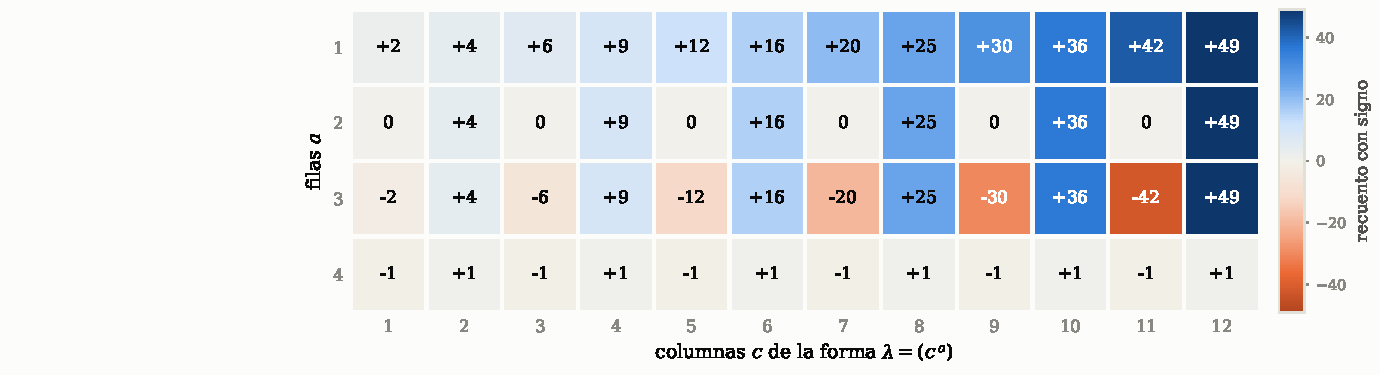
\includegraphics[width=\textwidth]{fig_signed_es.pdf}
\caption{Los recuentos con signo del Ejemplo \ref{ex:boxes}: el valor del Corolario \ref{cor:enum} en
$z=1$ y $t=2$ para las formas rectangulares $\lambda=(c^{\,a})$, esto es la $(-1)$-enumeración de
particiones planas en una caja $a\times(4-a)\times c$. Cada entrada es la forma cerrada
$\varepsilon_\lambda\,d_1d_2d_3/(2t^2)$, contrastada contra una enumeración directa de las tablas. La
fila $a=2$ se anula para $c$ impar y es un cuadrado perfecto para $c$ par.}
\label{fig:signed}
\end{figure}

La literatura de $(-1)$-enumeración calcula tales recuentos con signo, y conviene ser exacto en cómo,
porque la diferencia de aquí es estrecha. Kuperberg \cite{Kup02} pesa los objetos por $\pm1$
directamente. Eisenkölbl \cite{Eis07} especializa $x_i=(-1)^i$ en una identidad de funciones de Schur
del tipo que usó Stanley \cite{Sta86} ---identidad que allí se señala que es también
\cite[Cor.~7.3]{IOTZ06}--- y obtiene la $(-1)$-enumeración de las particiones planas
autocomplementarias con un lado impar. Ciucu y Krattenthaler evalúan los determinantes
correspondientes. En todos ellos el alfabeto es un número y no queda nada libre, que es el único
punto de diferencia: aquí el par recíproco mantiene viva una variable a lo largo del recuento con
signo. Eso lo hace el alfabeto, no un argumento nuestro.

En el mundo de las cintas hay un refinamiento de otra clase, y conviene decir cuál: los polinomios
LLT de Lascoux, Leclerc y Thibon \cite{LLT97} gradúan las tablas de cintas por un estadístico de
spin. Ese $q$ es una graduación añadida y no una letra, y el objeto que gradúa va indexado por una
tupla de formas; el parámetro de aquí es el del propio alfabeto y quien lo transporta es un solo
$s_\lambda$. Los dos refinan cosas distintas, y por eso enunciamos el punto de forma estrecha: es el
par recíproco, y no un estadístico, lo que mantiene viva una variable a través del recuento con
signo.

Una enumeración con signo que tiene fórmula de producto pide una involución que invierta el signo, y
el obstáculo es específico: la involución debe preservar $m_{t+1}-m_{t+2}$, o el parámetro libre no
se transporta, y ni los movimientos de Bender--Knuth ni el intercambio de una sola celda lo hacen.
La construcción de \cite{KumariThesis} de una involución sin puntos fijos que invierte el signo
sobre tablas semiestándar en un alfabeto emparejado por $\pm$, cuyo conjunto fijo son las tablas
embaldosables por dominós, sí tiene la propiedad requerida en su instancia $i=1$: toca solo celdas
que contienen $1$ o $2$, luego preserva $z^{m_3-m_4}$ e invierte $(-1)^{m_2}$. El producto triple
sobre el que tendría que aterrizar es el del Corolario \ref{cor:chars}, que en $t=2$ es sin más un
producto de tres caracteres $\mathfrak{sl}_2$, de modo que la biyección que falta es un enunciado de
Clebsch--Gordan. Esa es una mitad. La
otra es la cancelación a través de la partición del alfabeto, y en $t=2$ concierne a una única
familia de un parámetro. Por \eqref{eq:threestep} más abajo,
\[
s_\lambda(1,-1,z,\zb)=\sum_{\ell(\nu)\le2}s_{\lambda/\nu}(1,-1)\,\chi_{\nu_1-\nu_2}(z),
\]
y una involución que transporte el parámetro debe preservar $k=\nu_1-\nu_2$, porque ese es el índice
del carácter sobre el que se apoya su término. Para $k$ fijo las $\nu$ admisibles son exactamente
$(m+k,m)$ con $m\ge0$, de modo que esa cancelación es un enunciado sobre una sola palabra.

El tamaño de los términos es clásico. El teorema de Littlewood tiene forma sesgada ---$\varphi_t
s_{\lambda/\nu}$ se anula salvo que $\lambda/\nu$ sea embaldosable por $t$-cintas, y en otro caso es
un signo de cinta por un producto sobre el cociente---, debida a Macdonald \cite[p.~91]{Mac95} y
demostrada allí por la misma vía de Jacobi--Trudi que tomamos abajo; el caso en que $\nu$ es el
$t$-núcleo es de Farahat. En $t=2$ y sobre nuestro alfabeto da $\sigma_m\in\{0,\pm1\}$ de inmediato.
Lo que no es clásico es cómo se mueve el signo con $m$, y eso es lo que la involución necesita.

\begin{figure}[t]
\centering
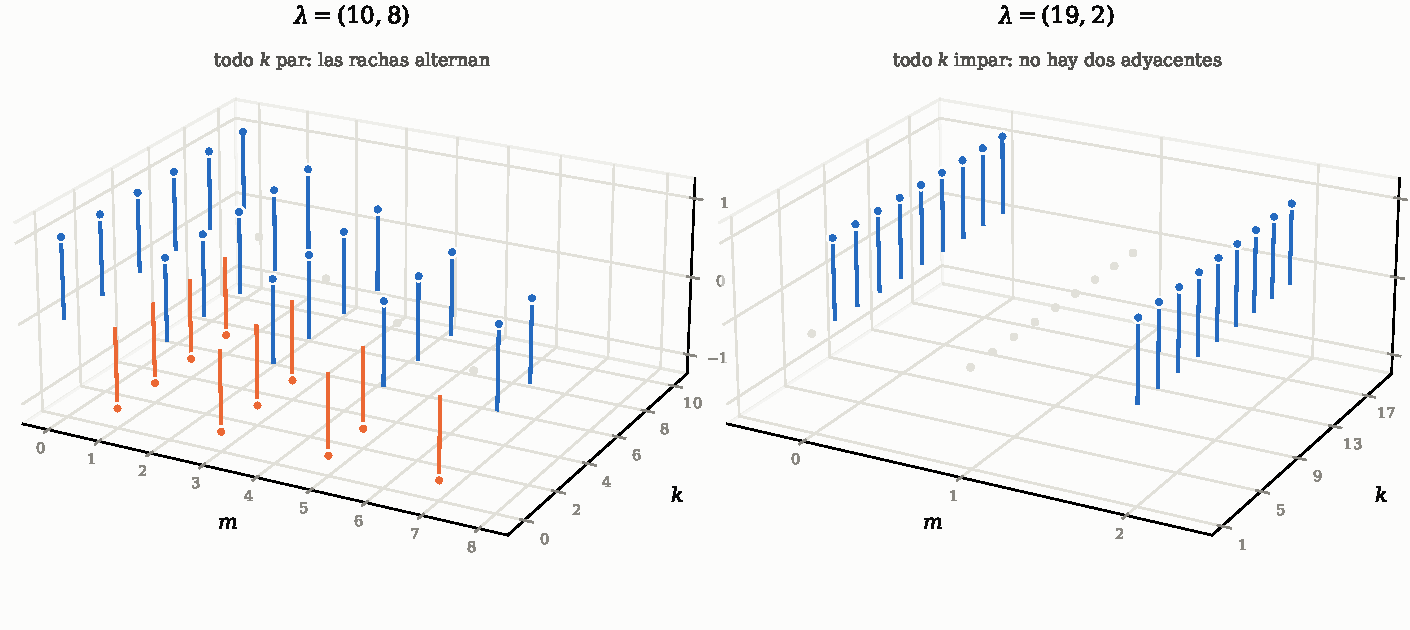
\includegraphics[width=\textwidth]{fig_runs_es.pdf}
\caption{La Proposición \ref{rem:involution}, dibujada. Para cada $k$ las $\nu$ admisibles son la
única familia $(m+k,m)$, y se representa $\sigma_m=s_{\lambda/(m+k,m)}(1,-1)$ frente a $m$ y $k$; los
puntos grises son los ceros. Toda barra tiene altura exactamente $\pm1$, que es la parte (i): los
términos forman un conjunto, luego la cancelación que pide la enumeración es un emparejamiento y no
algo con multiplicidad. A la izquierda todo $k$ es par y el color alterna a lo largo de cada racha,
que es la parte (iii) y lo que hace que $m\leftrightarrow m+1$ invierta el signo; donde una racha
acaba, la acaba un cero. A la derecha todo $k$ es impar y no hay dos términos no nulos contiguos,
que es la parte (ii): las rachas tienen longitud uno y no hay nada que cancelar.}
\label{fig:runs}
\end{figure}

\begin{proposition}[las rachas alternan]\label{rem:involution}
Sean $t=2$ y $k\ge0$, y sea $\sigma_m=s_{\lambda/(m+k,m)}(1,-1)$ para $m\ge0$. Entonces
\begin{enumerate}
\item[\rm(i)] $\sigma_m\in\{0,\pm1\}$ --- esta parte es de Macdonald y no nuestra;
\item[\rm(ii)] si $k$ es impar, no hay dos $\sigma_m$ consecutivos no nulos;
\item[\rm(iii)] si $\sigma_m$ y $\sigma_{m+1}$ son ambos no nulos, entonces
$\sigma_{m+1}=-\sigma_m$.
\end{enumerate}
En consecuencia, emparejar $m$ con $m+1$ dentro de cada racha maximal de $\sigma$ no nulos
consecutivos es una involución que invierte el signo, y $\sum_m\sigma_m$ es el recuento con signo de
las rachas de longitud impar.
\end{proposition}

Las tres partes se ven a la vez en la Figura \ref{fig:runs}: las alturas de las barras son la parte
{\rm(i)}, los huecos del panel impar son la parte {\rm(ii)}, y la alternancia del color a lo largo de
cada racha es la parte {\rm(iii)}.

\begin{proof}
Escribamos $\beta_i=\lambda_i-i$ y $c_j=\nu_j-j$, y tomemos la matriz de Jacobi--Trudi de
$s_{\lambda/\nu}$ con $n\ge\ell(\lambda)$ filas. Como $h_j(1,-1)=1$ para $j\ge0$ par y $0$ en otro
caso,
\begin{equation}\label{eq:betaJT}
M_{ij}=\bigl[\beta_i\ge c_j\bigr]\cdot\bigl[\beta_i\equiv c_j \bmod 2\bigr],\qquad
\sigma_m=\det M .
\end{equation}
El segundo factor dice que la columna $j$ está soportada en las filas de una sola clase de paridad,
la de $c_j$; y como $\beta_1>\dots>\beta_n$, dentro de esa clase el primer factor recorta un
\emph{segmento inicial}. Ordenando las filas por clase de paridad, $M$ queda diagonal por bloques,
de modo que es singular salvo que cada clase lleve tantas columnas como filas tiene, y dentro de una
clase es la escalera $\bigl[\,\text{el rango de }i\text{ en su clase}\le\ell_j\bigr]$ de las
longitudes $\ell_j$. Esa escalera es singular si dos longitudes coinciden o alguna es $0$, y en otro
caso las longitudes son una permutación de $1,\dots,e$ y su determinante es el signo de esa
permutación. Esto da (i), que en este caso es \cite[p.~91]{Mac95}; lo rededucimos porque la forma
$\beta$ \eqref{eq:betaJT} es lo que sostiene (ii) y (iii).

Para $\nu=(m+k,m)$ se tiene $c_1=m+k-1$, $c_2=m-2$ y $c_j=-j$ para $j\ge3$. Luego $c_1-c_2=k+1$, y
pasar de $m$ a $m+1$ sube $c_1$ y $c_2$ en uno y deja las demás columnas quietas: cambian de clase
de paridad exactamente las dos primeras.

Si $k$ es impar entonces $c_1\equiv c_2$, así que las columnas $1$ y $2$ están en la misma clase y
ambas la abandonan. El número de columnas de esa clase cambia en dos mientras que su número de filas
no, de modo que a lo sumo uno de $\sigma_m$, $\sigma_{m+1}$ puede ser no nulo, que es (ii).

Si $k$ es par entonces $c_1\not\equiv c_2$ y las dos columnas intercambian clase. Supongamos que
ambos son no nulos. En la clase de $c_1$ las columnas son la columna $1$ junto con un conjunto de
columnas $j\ge3$ que no se mueve; por (i) las longitudes son una permutación de $1,\dots,e$ antes y
después, y las columnas fijas aportan las mismas a ambas, luego la longitud que trae la columna $2$
es la que se llevó la columna $1$ ---y simétricamente en la otra clase. Cada clase ve por tanto las
mismas longitudes en el mismo orden de columnas, y los dos determinantes de bloque no cambian. Lo
que sí cambia es la baraja que separa las dos clases de columnas: las columnas $1$ y $2$ son
contiguas e intercambian pertenencia, lo que altera el número de inversiones de esa baraja en
exactamente uno. Luego $\sigma_{m+1}=-\sigma_m$, que es (iii).
\end{proof}

\begin{remark}[el signo de aquí es el signo del Teorema \ref{thm:main}]\label{rem:onesign}
Escribamos $\sigma_\nu$ para la permutación de la \S\ref{sec:background} asociada a una partición
$\nu$: la que ordena $\beta$ por clase de residuos, y que la Proposición \ref{rem:sign} coloca
dentro de $\varepsilon_\lambda$. Los términos de la Proposición \ref{rem:involution} son valores de
ese mismo signo. En efecto, $\sigma_m$ se anula salvo que $\core_2(\lambda)=\core_2(\nu)$ y ambas
componentes del $2$-cociente sesgado sean tiras horizontales, y vale
$\sgn(\sigma_\lambda)\sgn(\sigma_\nu)$ cuando no se anula ---siendo la identidad
$\sgn(\sigma_\lambda)\sgn(\sigma_\nu)=(-1)^{\sum_B\mathrm{ht}(B)}$ el signo de cintas de
\cite[p.~91]{Mac95} escrito como signo de ordenación, que es
\cite[Lema 6.3]{KumariThesis}. Las partes {\rm(ii)} y {\rm(iii)} son
entonces un único enunciado sobre $\sigma_\nu$ solo: al pasar $\nu=(m+k,m)$ a $(m+k+1,m+1)$,
$\sgn(\sigma_\nu)$ cambia de signo si $k$ es par y es constante si $k$ es impar. Así que la
permutación que lleva el signo del teorema principal es la permutación que hace alternar la
involución de esta sección; las dos mitades del artículo están firmadas por un mismo objeto.
\end{remark}

El emparejamiento es una biyección de tablas y no solo de términos, que es lo que transporta el
parámetro. Una tabla semiestándar de forma $(a,b)$ en las letras $3,4$ tiene segunda fila $4^{\,b}$
y primera fila $3^{\,p}4^{\,a-p}$ con $b\le p\le a$, de peso $z^{2p-a-b}$; añadirle una primera
columna $\left(\begin{smallmatrix}3\\4\end{smallmatrix}\right)$ la lleva a la tabla de forma
$(a+1,b+1)$ con $p+1$ en lugar de $p$, y $2(p+1)-(a+1)-(b+1)=2p-a-b$, de modo que $m_3-m_4$ se
preserva exactamente. Componer eso con la Proposición \ref{rem:involution} empareja los términos del
Corolario \ref{cor:enum} del modo que la enumeración pide.

Una mitad no es nuestra, y decimos cuál. La Proposición \ref{rem:involution} despacha la cancelación
a través de $\nu$; la cancelación \emph{dentro} de cada $s_{\lambda/\nu}(1,-1)$ es
\cite{KumariThesis}, y las dos encajan. Allí, con $n=1$, el alfabeto es $(x,-x)$ y el peso de un
llenado de dos letras es $(-1)^{c_2}$, que es $\sigma_m$; la involución
\cite[Lema 2.18]{KumariThesis} es libre de puntos fijos sobre los llenados \emph{no cubribles}, de
modo que la suma se reduce a los cubribles, que el \cite[Lema 2.16]{KumariThesis} pone en
correspondencia con tablas de dominó. Lo que hace utilizable la reducción aquí es el
\cite[Lema 2.14]{KumariThesis}: la paridad del número de dominós verticales no depende de la tabla,
luego toda superviviente lleva el mismo signo y $\sigma_m=\pm\#\{\text{llenados cubribles}\}$. Con la
parte (i), eso obliga al recuento a ser a lo sumo uno, así que el conjunto fijo es un único llenado
cuando $\sigma_m\ne0$ y vacío en otro caso ---comprobado directamente sobre las $1134$ formas
sesgadas con a lo sumo cuatro filas y $|\lambda|\le10$, donde los dos recuentos coinciden sin
excepción.

En $t=2$ existe por tanto la involución que la enumeración pide: cancelar dentro de cada $\nu$ por
el \cite[Lema 2.18]{KumariThesis}, emparejar lo que queda a través de $\nu$ por la Proposición
\ref{rem:involution}, y transportar el parámetro con la columna
$\left(\begin{smallmatrix}3\\4\end{smallmatrix}\right)$. Sus puntos fijos son un llenado por cada
racha de longitud impar, y el Corolario \ref{cor:enum} los cuenta. La construcción es de Kumari; el
ensamblaje es nuestro.

%======================================================================
\section{La factorización está aislada}\label{sec:sharp}

Una factorización solo es un resultado si no es especialización de otra conocida, y solo es un
resultado \emph{nítido} si el alfabeto no admite deformación. Eso no lo demostramos en general. Lo
que hacemos es probar cuatro deformaciones de \eqref{eq:object}, y las cuatro destruyen el producto.

La evidencia de esta sección es computacional, y así la etiquetamos: ninguna de (D1)--(D4) es un
teorema, y en particular no demostramos ningún resultado de imposibilidad. Lo que afirmamos es que la
identidad \eqref{eq:main} es falsa para cada alfabeto deformado, cosa que zanja un solo
contraejemplo, y damos recuentos para indicar cuán lejos está de ser cierta.

\begin{itemize}
\item[\rm(D1)] \emph{Más pares recíprocos.} Para
$s_\lambda(\zt,z_1,z_1^{-1},\dots,z_r,z_r^{-1})$
la ley de producto del Teorema \ref{thm:main} ya falla en $r=2$: en el rango calculado los valores
típicos llevan un factor irreducible grande, y los únicos
factores que se observa que se desprendan son binomios en las variables rotadas $z_1z_2$ y $z_1z_2^{-1}$, esto es,
los acoplamientos entre las cargas $u(1)$ de los pares. Lo que sí sobrevive es el \emph{lugar de
anulación}: en $t=2$ sobrevive a todo $r$ y el Teorema \ref{conj:crit} lo determina por completo,
mientras que para $t$ y $r$ arbitrarios el Teorema \ref{thm:suff} da un criterio suficiente uniforme
y la Conjetura \ref{conj:general} es el recíproco. Con esta evidencia el producto parece un accidente
de rango uno y la anulación la parte que generaliza; la primera mitad de esa frase es la Conjetura
\ref{conj:rank2} y sólo la segunda es un teorema.
\item[\rm(D2)] \emph{Más variables en la órbita.} Para
$s_\lambda(X,\zeta X,\dots,\zeta^{t-1}X,z,z^{-1})$ la ley de producto ya falla en $|X|=n=2$. Con $t=2$,
$n=2$ el valor para $\lambda=(2)$ es $(x^2z^2+y^2z^2+z^4+z^2+1)/z^2$, irreducible sobre $\mathbb Q$;
para $\lambda=(2,2)$ es $(x^2+y^2+z^2)(x^2z^2+y^2z^2+1)/z^2$, dos factores en lugar de tres; y para
$\lambda=(3,1)$ es de nuevo irreducible. En cambio, suprimido el par, el mismo alfabeto obedece
\cite[Teorema 2.3]{AK25}: $s_{(2)}(x,y,-x,-y)=x^2+y^2$ y $s_{(2,2)}(x,y,-x,-y)=(x^2+y^2)^2$.
\item[\rm(D3)] \emph{La órbita sustituida por una clase lateral.} Para $\zeta'\zt$ con
$\zeta'=e^{\pi i/t}$, las potencias impares de una raíz $2t$-ésima primitiva de la unidad ---el
torcimiento de \cite[\S3]{AK25}, y para $t$ par el conjunto completo de raíces $2t$-ésimas primitivas
estudiado en \cite{HI24}--- la identidad falla, criterio de anulación incluido.
\item[\rm(D4)] \emph{El par recíproco sustituido por un par libre.} $s_\lambda(\zt,x,y)$ resultó
irreducible en todos los casos que calculamos. No afirmamos nada fuera de ese rango.
\end{itemize}

Recuentos para (D3) y (D4), sobre $t=2,\dots,6$ y $|\lambda|\le10$: la identidad se cumple en los
$600$ casos para \eqref{eq:object}, en $383$ de $600$ para (D3) y en $200$ de $600$ para (D4). El
contraste es por tanto capaz de fallar, que es la razón de citar la primera fila.

Una sola lectura de la demostración explica las cuatro. Partiendo el alfabeto y aplicando el Teorema
\ref{thm:LR} a la mitad congelada se obtiene, para cualquier alfabeto libre $B$,
\begin{equation}\label{eq:threestep}
s_\lambda(\zt\cup B)=\sum_{\nu}s_{\lambda/\nu}(\zt)\,s_\nu(B)=\sum_\nu\varepsilon_\nu\,s_\nu(B),
\qquad \varepsilon_\nu\in\{0,\pm1\},
\end{equation}
siendo los coeficientes signos de cinta: que la evaluación sesgada $s_{\lambda/\nu}(\zt)$ sea $0$ o
un signo de cinta es la forma sesgada del Teorema \ref{thm:LR}, debida a Macdonald
\cite[p.~91]{Mac95}. Ahora bien, $B=(z,z^{-1})$ tiene exactamente dos letras y
son recíprocas, luego $s_\nu(B)=\chi_{\nu_1-\nu_2}(z)$ es un \emph{único} carácter
$\mathfrak{sl}_2$ que depende de una sola diferencia, y la suma corta con signos colapsa. El primer
paso exige que la mitad congelada sea una órbita completa, pues el Teorema \ref{thm:LR} necesita que
las filas toquen cada clase de residuos exactamente; una clase lateral no lo hace, y eso es (D3). El
segundo paso exige que la mitad libre sea exactamente un par recíproco: un par libre tiene
$\det=xy$ y se acopla a las dos cargas centrales, y eso es (D4), mientras que agrandar la mitad libre
---con más pares, o con más variables en la órbita, lo que agranda $\nu$--- hace que $s_\nu(B)$ deje
de ser un único carácter y que la suma deje de colapsar, y eso es (D1) y (D2). \emph{Los cuatro
fallos son una sola condición vista desde cuatro lados.}

\begin{remark}
Equivalentemente: el par recíproco aporta exactamente \emph{un} acoplamiento, el término cruzado
$d_3$, porque $\det=1$ le impide ver por separado las dos cargas centrales. Por eso hay tres factores
y no dos, y las factorizaciones de Ayyer--Kumari, que son productos sobre componentes del cociente
sin acoplamiento alguno, son el caso en que esa aportación está ausente.
\end{remark}

\begin{remark}[una lectura teórico-representacional]\label{rem:twining}
El alfabeto \eqref{eq:object} es cerrado bajo inversión, luego es un elemento del toro de $O(N)$, y
su determinante es $(-1)^{t+1}$. Para $t$ par está por tanto en la componente no identidad, donde un
carácter es un carácter \emph{twining}; la identidad que calcula tales caracteres por plegado se debe
a Jantzen \cite{Jantzen} y, en la forma más próxima a esta, a Kumar--Lusztig--Prasad \cite{KLP},
siendo el álgebra plegada relevante el álgebra órbita. Nuestra restricción es reducible, de modo que
se llega a ella desde la suya con un paso de teoría de Clifford. Lo registramos porque
Ciucu--Krattenthaler \cite{CK09} escribieron que no podían ofrecer una interpretación
teórico-representacional de sus factorizaciones, y \cite{AB19} y \cite{AK25} registran que sigue
faltando; la lectura de aquí es de esa clase. El mecanismo es enteramente suyo, y la demostración
anterior no lo usa. El Lema \ref{lem:AtoSp} concreta esa lectura para el alfabeto \eqref{eq:psir},
donde el álgebra plegada es $C_r$ y el carácter twining es un carácter simpléctico sin más.
\end{remark}

%======================================================================
\section{El lugar de anulación sobrevive a todo $r$}\label{sec:zeros}

Esta sección está más allá de la factorización, y se lee distinto de las siete anteriores. Aquéllas
demuestran enunciados sobre una identidad; ésta pregunta qué queda cuando la identidad ya no está, y
la respuesta es un lugar geométrico y no una fórmula ---demostrado en un sentido para todo $r$, y en
el otro solo hasta donde hemos podido llegar. El cambio de registro es el asunto que cambia, no el
listón.

Por (D1), el producto del Teorema \ref{thm:main} no sobrevive a un segundo par recíproco. Su
\emph{lugar de anulación} sí, y para todo $r$ admite forma cerrada. Escribamos
\begin{equation}\label{eq:psir}
\Psi_r(\lambda)\;:=\;s_\lambda(1,-1,z_1,\bar z_1,\dots,z_r,\bar z_r),\qquad N=2r+2,
\end{equation}
de modo que $\Psi_1$ es \eqref{eq:object} en $t=2$. En toda esta sección $\lambda$ se completa con
ceros hasta tener exactamente $N$ partes, $\beta=\beta(\lambda)$ es su conjunto beta y $E$ y $O$ son
sus entradas pares e impares. Diremos que $\lambda$ es \emph{autocomplementaria de anchura $w$} si
$\lambda_i+\lambda_{N+1-i}=w$ para todo $i$, en cuyo caso $w=\lambda_1+\lambda_N$. Las dos
condiciones que gobiernan la sección son
\begin{equation}\label{eq:branches}
\boxed{\;\;
\underbrace{|E|\in\{0,N\}}_{\text{rama (a)}}
\qquad\qquad
\underbrace{\lambda_i+\lambda_{N+1-i}=w\ \ \text{para todo }i,\ \ w\ \text{impar}}_{\text{rama (b)}}
\;\;}
\end{equation}
La rama (a) dice que el conjunto beta tiene paridad constante; la rama (b), que $\lambda$ es
autocomplementaria de anchura impar.

Enunciamos las cuatro afirmaciones por separado, porque no están demostradas en la misma medida y un
único bicondicional lo ocultaría.

\begin{theorem}[las dos ramas]\label{thm:zeros}
Para todo $r\ge1$ y toda $\lambda$: si se cumple la rama {\rm(a)} o la rama {\rm(b)}, entonces
$\Psi_r(\lambda)=0$.
\end{theorem}

\begin{corollary}\label{cor:sizes}
Si $\lambda$ es autocomplementaria de anchura impar $w$, entonces $|\lambda|=w(r+1)$. En particular
la rama {\rm(b)} solo puede darse para $|\lambda|\equiv r+1 \pmod{2(r+1)}$, y un tamaño fuera de esa
progresión no necesita más comprobación.
\end{corollary}

\begin{proof}
Sumar $\lambda_i+\lambda_{N+1-i}=w$ sobre $i$ cuenta $|\lambda|$ dos veces, luego
$2|\lambda|=wN=w(2r+2)$.
\end{proof}

La progresión se ve en la Figura \ref{fig:zeros}, y merece la pena dejar constancia de que el
enunciado análogo para el lugar entero es falso: la rama {\rm(a)} no está confinada a ella, y por eso
la condición hay que leerla sobre la rama {\rm(b)} sola.

\begin{figure}[!ht]
\centering
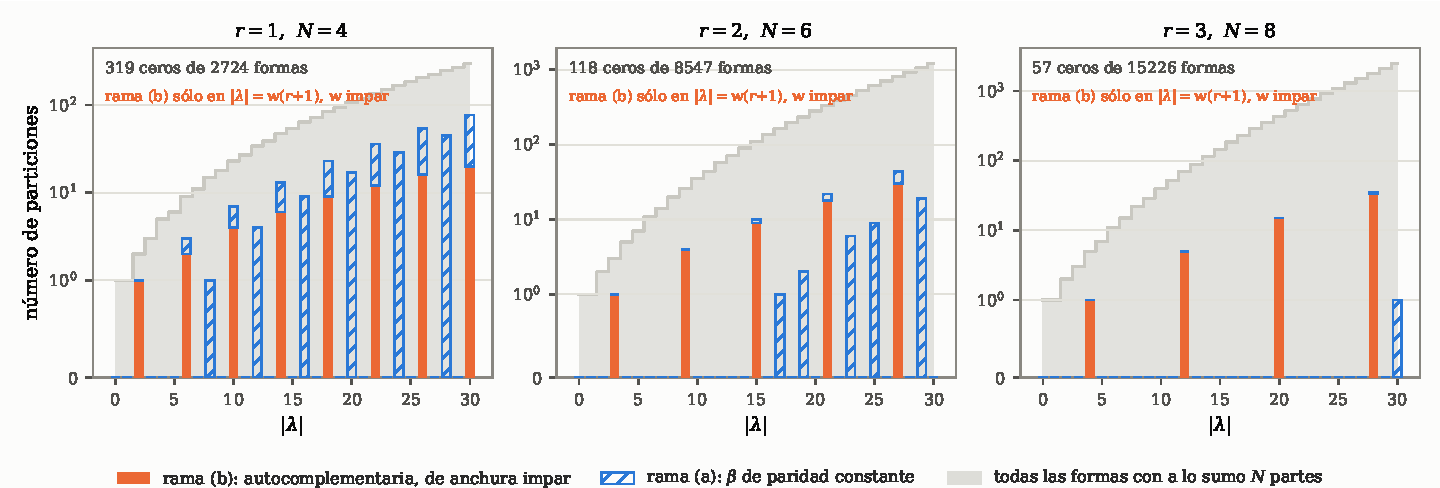
\includegraphics[width=\textwidth]{fig_zeros_es.pdf}
\caption{El lugar de anulación del Teorema \ref{thm:zeros}, contado en lugar de dibujado. Para cada
tamaño $|\lambda|$ las barras dan el número de particiones con a lo sumo $N$ partes que se anulan,
separadas por rama; el escalón sombreado es el número total de formas de ese tamaño, en el mismo eje,
de modo que la rareza del lugar se ve y no se afirma. Los tamaños que llevan la rama (b) son
exactamente los múltiplos $w(r+1)$ con $w$ impar, por el Corolario \ref{cor:sizes}; la rama (a) ocupa
otros tamaños y necesita que el conjunto beta se salte una paridad por completo, razón por la cual
está ausente en $|\lambda|$ pequeño en cuanto $N$ crece.}
\label{fig:zeros}
\end{figure} Conviene dejar constancia de que el enunciado
análogo para todo el lugar de anulación es falso: la rama (a) no está confinada a esa progresión, y
por eso la condición hay que leerla de la rama (b) sola.

\begin{theorem}[un par]\label{thm:r1}
Para $r=1$ vale también el recíproco: $\Psi_1(\lambda)=0$ solo si se cumple {\rm(a)} o {\rm(b)}.
\end{theorem}

\begin{theorem}[dentro del rango de Littlewood]\label{thm:stable}
Para todo $r$ y toda $\lambda$ con $\ell(\lambda)\le N/2$ vale el recíproco. Equivalentemente, en ese
rango $\Psi_r(\lambda)=0$ si y solo si $\lambda=(k^{\,N/2})$ con $k$ impar.
\end{theorem}

\begin{remark}[los rectángulos son donde se detienen los argumentos generales]
Vale la pena advertir que los dos sitios donde falla un argumento general de este artículo son
rectángulos, a dos alturas distintas y por dos razones distintas. A altura $N/2$ un rectángulo impar
es autocomplementario de anchura impar, luego se anula; por el Teorema \ref{thm:stable} son las
únicas formas del rango de Littlewood que lo hacen, y en la demostración son precisamente aquellas
para las que no se puede construir el testigo asociado. A altura completa el objeto no se anula, sino
que degenera en sentido contrario: $s_{(c^{\,N})}(x)=(x_1\cdots x_N)^{c}$ es un monomio, de modo que
sobre cualquier alfabeto $A$ el valor es $\det(A)^{c}$ y de la forma no sobrevive nada ---que con
$t=2$ es el caso {\rm(i)} de la Proposición \ref{prop:rect}, el único allí en el que la paridad de
$c$ no interviene---. Entre ambas alturas el argumento genérico se aplica sin cambios. Los
rectángulos no son una molestia que haya que tratar caso por caso: son el borde de la forma, y cada
uno de los dos extremos rompe una hipótesis distinta ---el primero la existencia de un testigo, el
segundo la no degeneración del triple de intervalos---.
\end{remark}

\begin{theorem}[el criterio en general]\label{conj:crit}
Para todo $r$ y toda $\lambda\in\PP_N$, $\Psi_r(\lambda)=0$ si y solo si se cumple {\rm(a)} o
{\rm(b)}.
\end{theorem}

\noindent Demostrado al final de la \S\ref{sec:zeros}, módulo el Teorema \ref{thm:PvW}.

Los Teoremas \ref{thm:zeros}--\ref{thm:stable} se demuestran en las
\S\S\ref{sec:brancha}--\ref{sec:conv}, y el Teorema \ref{conj:crit} --- el criterio para todo
$r$ --- al final de esta sección, por una vía independiente de los tres. Lo enunciamos aparte por dos
razones. Es el único resultado del artículo que se apoya en algo ajeno, el Teorema
\ref{thm:PvW}; y las dos vías que llevan a él no son la misma vía. La de Littlewood lo reduce, en la
\S\ref{sec:unstable}, a un único enunciado de existencia, y esa reducción no se completa: el rango
$\ell(\lambda)>N/2$ es exactamente donde la regla de restricción deja de aplicarse y, aunque el
Lema \ref{lem:AtoSp} resuelve allí los valores, el enunciado sobre los coeficientes no --- el
certificado que propusimos para él falla, por la Proposición \ref{conj:iso}. El argumento extremal
de las \S\S\ref{sec:extremal} y \ref{sec:rigidity} no entra en ese rango en absoluto: trabaja en
la filtración por grados del numerador y no se cruza jamás con un coeficiente de Littlewood.

Leído sobre el grupo y no sobre el alfabeto, el mismo teorema describe una propiedad de rigidez, y lo
enunciamos aparte porque es la forma en que lo querría alguien de teoría de representaciones. La
traducción no es nuestra ni es nueva: que una representación de $O(N)$ sea estable por $\det$
exactamente cuando su carácter se anula fuera de la componente identidad es elemental, y que eso sea
la condición $m_\nu=m_{\nu^{*}}$ sobre los asociados de Littlewood \cite{Lit50} es clásico. El
corolario reclama por tanto exactamente lo que reclama el Teorema \ref{conj:crit}, y nada más.

\begin{corollary}[rigidez frente al giro por el determinante]\label{cor:dettwist}
Sean $N=2r+2$ y $\lambda\in\PP_N$, y sea $V_\lambda$ el $GL(N)$-módulo polinómico irreducible de peso
máximo $\lambda$. Entonces
\[
V_\lambda\big|_{O(N)}\;\cong\;V_\lambda\big|_{O(N)}\otimes\det
\]
si y solo si $\beta(\lambda)$ tiene paridad constante, o $\lambda$ es autocomplementaria de anchura
impar. Equivalentemente: \eqref{eq:branches} clasifica exactamente los $GL(N)$-módulos polinómicos
irreducibles cuya restricción a $O(N)$ es estable por el carácter del grupo de componentes.
\end{corollary}

\begin{proof}
En característica $0$ un $O(N)$-módulo de dimensión finita es semisimple y queda determinado por su
carácter, así que para $W=V_\lambda|_{O(N)}$ se tiene $W\cong W\otimes\det$ si y solo si
$\chi_W=\chi_{W\otimes\det}$. Esos dos caracteres coinciden automáticamente en la componente
identidad, y en la otra $\chi_{W\otimes\det}=-\chi_W$; luego la condición es que $\chi_W$ se anule en
$O(N)^{-}$. Todo elemento \emph{semisimple} de $O(N)^{-}$ es conjugado a uno de espectro
$(1,-1,z_1^{\pm1},\dots,z_r^{\pm1})$, que es el alfabeto de \eqref{eq:psir}; y como los semisimples
son densos en $O(N)^{-}$ y $\chi_W$ es regular, anularse en ese toro es anularse en toda la
componente. La condición es por tanto $\Psi_r(\lambda)\equiv0$, y el Teorema \ref{conj:crit} es el
criterio. El diccionario entre las dos lecturas es la expansión por asociados de Littlewood, recordada
en la \S\ref{sec:conv}.
\end{proof}

\noindent El crédito se reparte exactamente igual que en el Teorema \ref{conj:crit}, y conviene
repetirlo aquí porque el lenguaje de grupos puede hacer que un enunciado conocido parezca nuevo. Que
las dos familias \eqref{eq:branches} \emph{sean} estables por $\det$ no es nuestro: en el extremo de
la familia, la primera es de Karmakar \cite[Teorema 4.1(A)]{Kar24}, y la segunda es la complementación
sobre la familia de índices de Ayyer y Behrend \cite{AB19}, como recoge \eqref{eq:compl}. Lo que el
Teorema \ref{conj:crit} añade, y es todo lo que añade, es que no hay ninguna más.

\begin{remark}[lo que el núcleo ve, y lo que no]\label{rem:core}
La rama (a) es una condición sobre el núcleo, y sencilla: con un número $N$ fijo de números beta, el
perfil de residuos determina $\core_t(\lambda)$ ---es la coordenada de Garvan--Kim--Stanton
\cite{GKS90}---, de modo que toda condición sobre el perfil lo es sobre el núcleo. No es, sin
embargo, la anulación del núcleo sino su extremo opuesto: en $t=2$ la rama (a) dice
\[
\core_2(\lambda)=(N-1,N-2,\dots,1)\qquad\text{o}\qquad\core_2(\lambda)=(N,N-1,\dots,1),
\]
los dos $2$-núcleos más grandes que admiten $N$ números beta, mientras que
$\core_2(\lambda)=\varnothing$ es el perfil equilibrado. La rama (b) no mueve ni el perfil ni el
núcleo, y por tanto le es invisible. En consecuencia $\core_2$ \emph{no} determina si $\Psi_r$ se
anula, y el testigo más pequeño es el propio núcleo vacío: entre las formas con
$\core_2(\lambda)=\varnothing$ en $r=1$,
\[
(1,1),\ (3,3),\ (2,2,1,1),\ \dots\quad\text{se anulan, y}\quad
\varnothing,\ (2),\ (1^4),\ \dots\quad\text{no,}
\]
y el mismo corte ocurre en $r=2$ y $r=3$, allí también en las clases de núcleo $(1)$, $(2,1)$ y
$(3,2,1)$: sobre los rangos de la \S\ref{sec:verif} hay cinco clases de núcleo que llevan ambos
comportamientos, y el perfil determina el núcleo sin ninguna colisión sobre $260$ perfiles con
$t\le5$. No puede existir, pues, ninguna reformulación del Teorema \ref{thm:zeros} en términos de
$\core_2(\lambda)$: el criterio necesita la forma y no solo su núcleo. Leídos contra el Teorema
\ref{thm:LR}, donde el núcleo vacío es exactamente lo que decide, los dos criterios discrepan en
ambas direcciones ---$(1,1)$ tiene $2$-núcleo vacío y $\Psi_1=0$, mientras que $(1)$ tiene
$2$-núcleo no vacío y $\Psi_1\ne0$.
\end{remark}

La familia de índices de (b) no es nueva: es precisamente la que Ayyer y Behrend destacan
\cite[observación tras el Teo.~3]{AB19}, junto con la obstrucción de paridad que registran allí ---una
partición no puede ser autocomplementaria en un rectángulo $a\times b$ con $a$ y $b$ ambos impares, y
aquí $a=N$ es par, luego el caso admisible es $b=w$ impar. Lo que sus teoremas dicen de esas formas es
que el carácter \emph{factoriza}; allí el alfabeto lleva el punto fijo $+1$ y tiene determinante $+1$.
El nuestro lleva $+1$ y $-1$, y tiene determinante $-1$.

\keybox{Sobre la \emph{misma} familia de formas, el alfabeto de determinante $+1$ hace que el
carácter factorice y el de determinante $-1$ hace que se anule. Una letra separa una factorización de
una aniquilación, y quien decide es el determinante del alfabeto; la identidad \eqref{eq:compl} de
más abajo es donde ocurre la separación.}


\subsection{Rama (a): el alfabeto al cuadrado}\label{sec:brancha}

Esta rama es de Karmakar, en el extremo. \cite[Teorema 4.1(A)]{Kar24} evalúa un carácter de
$\mathrm{GL}(n,\CC)$ en $C_{n-k,k}=(1,\dots,1,-1,\dots,-1)$ y da
$\chi_\lambda(C_{n-k,k})=0$ cuando $\#\eta_0(\lambda)>n-k$, donde su
$\eta_i(\lambda)=\{a\in\lambda+\rho: a\equiv i \bmod 2\}$ es exactamente la partición de
$\beta(\lambda)$ en $E$ y $O$ que usamos aquí; en $k=1$, tras su normalización por el carácter
determinante, eso es la rama (a). El argumento de una línea que sigue se incluye porque es el que
reutiliza el resto de la sección, no porque sea nuevo.

\begin{proof}[Demostración del Teorema \ref{thm:zeros}, rama {\rm(a)}]
Sea $A=\{1,-1,z_1,\bar z_1,\dots\}$. Si $\beta=2\gamma$, entonces
$\det(a^{\beta_j})_{a\in A}=\det\big((a^2)^{\gamma_j}\big)_{a\in A}$, y si $\beta=2\gamma+1$ ocurre lo
mismo tras extraer $\prod_{a\in A}a$. En ambos casos el bialternante factoriza a través del alfabeto
al cuadrado $A^2=\{1,1,z_1^{2},\bar z_1^{2},\dots\}$, en el que la letra $1$ aparece dos veces porque
$1^2=(-1)^2$. Hay dos filas iguales.
\end{proof}

\subsection{Rama (b): una torsión por el determinante, y autodualidad}

\begin{proof}[Demostración del Teorema \ref{thm:zeros}, rama {\rm(b)}]
Sea $\hat\lambda$ el complementario de $\lambda$ en la caja $w\times N$, leído del revés. En
conjuntos beta, $\beta(\hat\lambda)=c-\beta(\lambda)$ recorrido en sentido inverso, con $c=w+N-1$, y
$\hat\lambda$ es el peso máximo de $V_\lambda^{*}\otimes\det^{\,w}$ como $\mathrm{GL}(N)$-módulo. Si
$\lambda=\hat\lambda$, entonces $V_\lambda\cong V_\lambda^{*}\otimes\det^{\,w}$. Restrinjamos a
$O(N)$: toda representación de $O(N)$ es autodual, luego
$V_\lambda|_{O(N)}\cong V_\lambda^{*}|_{O(N)}\cong V_\lambda|_{O(N)}$, de donde
\[
V_\lambda|_{O(N)}\;\cong\;V_\lambda|_{O(N)}\otimes\det^{\,w}.
\]
El alfabeto \eqref{eq:psir} es un elemento del toro de la componente $\det=-1$, así que para $w$
impar la torsión es por $\det$ mismo y el carácter se anula ahí. Para $w$ par, $\det^{\,w}$ es
trivial y el argumento no da nada: por eso la paridad de $w$ no es un adorno.
\end{proof}

Equivalentemente, y esto es el cálculo en lugar de la representación, la identidad de complementación
estándar da
\begin{equation}\label{eq:compl}
s_{\hat\lambda}(A)\;=\;\Big(\textstyle\prod_{a\in A}a\Big)^{c}\,(-1)^{\binom{N}{2}}(-1)^{r}\,
s_\lambda(A)\;=\;(-1)^{c}\,(-1)\,s_\lambda(A),
\end{equation}
usando que $A$ es cerrado por inversión ---$A^{-1}$ es $A$ con los $r$ pares recíprocos
transpuestos, lo que aporta $(-1)^r$--- y que $\prod_{a\in A}a=-1$. Con $c$ par esto se lee
$s_{\hat\lambda}=-s_\lambda$, y una forma autocomplementaria queda aniquilada. La rama (b) del
Teorema \ref{thm:zeros} es por tanto un corolario de dos líneas de una identidad de manual sobre una
familia de índices conocida, y no la reclamamos como nada más. La Figura \ref{fig:involution} dibuja
el emparejamiento que hace la identidad, y a su lado la misma forma con una caja movida, donde el
emparejamiento se rompe; el contenido de la sección es el recíproco.

\subsection{El recíproco}\label{sec:conv}

\begin{figure}[t]
\centering
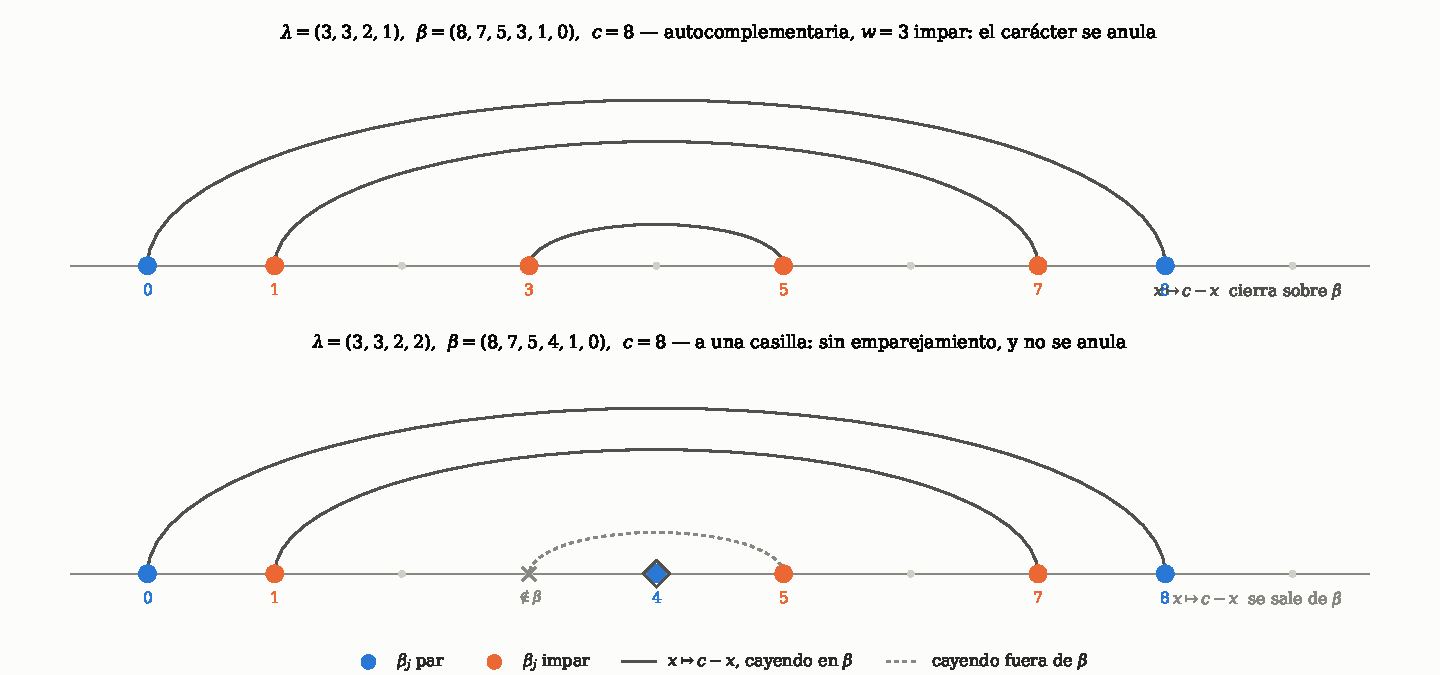
\includegraphics[width=\textwidth]{fig_involution_es.pdf}
\caption{Por qué la autocomplementariedad mata el carácter. Al desarrollar por las dos filas
congeladas quedan términos indexados por pares $(e,o)$ con $e\in E$, $o\in O$, y la reflexión
$x\mapsto c-x$ actúa sobre ellos. Arriba, una forma autocomplementaria de anchura impar: todo arco
cae dentro de $\beta$ y une entradas de igual paridad, porque $c$ es par. Abajo, la misma forma con
una caja movida: el arco $5\mapsto3$ se sale de $\beta$, así que no hay emparejamiento y nada se
cancela. El rombo marca el punto fijo de la reflexión, que no puede darse dentro de un par de
paridades opuestas ---y ésa es la razón de que la involución sea libre.}
\label{fig:involution}
\end{figure}

\begin{proof}[Demostración del Teorema \ref{thm:r1}]
Pongamos $c_\ast=z+\bar z$ y definamos $S_n$ por $S_0=0$, $S_1=1$, $S_{n+1}=c_\ast S_n-S_{n-1}$, de
modo que $\deg_{c_\ast}S_n=n-1$ y $S_{-n}=-S_n$; el valor $S_{-1}=-1$ se usa siempre que
$\beta_N=0$. Como $\Phi_A=(x^2-1)(x^2-c_\ast x+1)$, un polinomio $P$ soportado en $\beta$ es
divisible por $\Phi_A$ exactamente cuando $P(1)=P(-1)=0$ y $P\equiv0$ módulo $x^2-c_\ast x+1$.
Separando $P(\pm1)$ por paridad y reduciendo $x^n\equiv S_nx-S_{n-1}$, la admisibilidad se convierte
en la singularidad de la matriz $4\times4$ con filas $[\beta_j\ \mathrm{par}]$,
$[\beta_j\ \mathrm{impar}]$, $S_{\beta_j}$, $S_{\beta_j-1}$. Desarrollando por las dos filas de
paridad y usando la identidad de d'Ocagne \cite{Doc} para esta recurrencia,
\begin{equation}\label{eq:docagne}
S_bS_{b'-1}-S_{b'}S_{b-1}=-S_{b-b'},
\end{equation}
cada bloque $2\times2$ colapsa a un \emph{único} $S$, indexado por la diferencia de los dos $\beta$
supervivientes. Los $S_n$ distintos tienen grados distintos en $c_\ast$ y son por tanto linealmente
independientes, de modo que la suma con signo se anula solo mediante un emparejamiento exacto de
índices iguales con signos opuestos. El análisis de casos es finito: $|E|\in\{0,4\}$ es la rama (a);
$|E|\in\{1,3\}$ deja tres términos cuyos índices son las tres diferencias dos a dos de un conjunto de
tres elementos y por tanto siempre distintas, así que no existe emparejamiento y el valor no es nulo;
y para $|E|=2$ hay cuatro términos y tres emparejamientos perfectos, y se comprueban los seis
patrones de paridad directamente. Para $E=\{\beta_1,\beta_4\}$ y para $E=\{\beta_2,\beta_3\}$ solo
uno de los tres emparejamientos está disponible, e impone la única condición
$\beta_1+\beta_4=\beta_2+\beta_3$, que es la rama (b); para los cuatro patrones restantes, cada uno
de los tres emparejamientos obliga a dos entradas distintas de $\beta$ a coincidir, así que ninguno
está disponible y el valor no es nulo.
\end{proof}

La identidad \eqref{eq:docagne} es clásica. El colapso que produce es un accidente de rango uno: dos
letras admiten un solo hueco, luego $s_{(m,n)}(z,\bar z)=S_{m-n+1}$ depende solo de ese hueco. No hay
análogo de rango $r$. Lo habría si existiera una forma cerrada de $s_\mu$ en alfabeto recíproco para
\emph{toda} $\mu$; \cite{CK09} la dan para formas rectangulares y \cite{AB19} para las
autocomplementarias, y nadie en general.

Para $r$ general usamos asociados, en el sentido de Littlewood \cite{Lit50}.
En el coset $\det=-1$, la relación $[\nu^{*}]=[\nu]\otimes\det$ da
$\Psi_r=\sum_\nu\big(m_\nu-m_{\nu^{*}}\big)\chi_{[\nu]}$, luego $\Psi_r=0$ si y solo si
$m_\nu(\lambda)=m_{\nu^{*}}(\lambda)$ para toda $\nu$; equivalentemente, si y solo si
$V_\lambda|_{O(N)}$ es invariante por $\det$. Esa equivalencia es el diccionario a través del cual se
lee el Corolario \ref{cor:dettwist}, y es lo que convierte el criterio en un enunciado sobre módulos
y no sobre un alfabeto. Un testigo es por tanto una sola $\nu$ con
$m_\nu\ne m_{\nu^{*}}$, y se puede construir.

El \cite[Teorema 4.1]{Kar24} de Karmakar determina el valor en el extremo $z_i=1$, que es un elemento
de orden dos: el caso (A) es la rama (a), el caso (B) es una dimensión no nula, y el caso (C) deja una
suma alternante de productos de dimensiones sin criterio de anulación asociado. La rama (b) vive en
ese caso (C), de modo que el teorema siguiente no es consecuencia suya. Y el caso (B) tampoco ayuda
más al crecer $r$: con $k=1$ pide que $N-1$ de los $N$ números beta compartan paridad, y la forma más
pequeña que lo hace es la escalera $(2r-1,2r-2,\dots,1)$, de tamaño $r(2r-1)$, así que sobre un rango
fijo de $|\lambda|$ su caso de no anulación sólo se ve para $r$ pequeño --- su resultado es más
afilado exactamente donde el nuestro es más fácil. Lo que conecta el extremo con
la curva es la rigidez, y la rigidez es un enunciado sobre nuestro objeto y no sobre el elemento de
orden dos: sobre los rangos de la \S\ref{sec:verif} se cumple en $\ell(\lambda)\le N/2$ sin excepción
y falla fuera, que es la Observación \ref{rem:rankone}.

\begin{proof}[Demostración del Teorema \ref{thm:stable}]
La rama (a) no puede darse: con $\ell(\lambda)\le N/2$ se anulan al menos dos partes finales, luego
$\beta$ contiene dos enteros consecutivos. En el rango de Littlewood,
$m_\nu(\lambda)=\sum_{\beta'\ \mathrm{par}}c^{\lambda}_{\nu\beta'}$, y el término
$\beta'=\emptyset$ da $m_\mu\ge1$ para toda $\mu\subseteq\lambda$. Tomemos $\mu$ así. Si
$\ell(\lambda)<N/2$, tomamos $\mu=\lambda$: entonces
$\ell(\lambda^{*})=N-\ell(\lambda)>\ell(\lambda)$, luego $\lambda^{*}\not\subseteq\lambda$ y
$m_{\lambda^{*}}=0\ne m_\lambda$. Si $\ell(\lambda)=N/2$ y $\lambda_{N/2}$ es par, tomamos
$\mu=(\lambda_1,\dots,\lambda_{N/2-1})$; entonces $\beta'=(\lambda_{N/2})$ es par, $\lambda/\mu$ es
una tira horizontal y $m_\mu\ge1$ con $\ell(\mu)<N/2$, así que se aplica a $\mu$ el cálculo anterior.
Si $\ell(\lambda)=N/2$ y $\lambda$ no es un rectángulo, sea $j\le N/2-1$ el mayor índice con
$\lambda_j>\lambda_{j+1}$ y quitemos la última fila y además una caja de la fila $j$; entonces
$\beta'=(\lambda_{N/2}+1)$ es par y $\lambda_j\ge\lambda_{N/2}+1$ mantiene $\lambda/\mu$ como tira
horizontal. Un rectángulo par $\lambda=(k^{\,N/2})$ ya lo cubre la segunda construcción, de modo que
el único caso que queda es $k$ impar, donde no está disponible ninguna de las dos construcciones
---y eso es la rama {\rm(b)}---.
\end{proof}

\subsection{Fuera del rango de Littlewood}\label{sec:unstable}

Para $\ell(\lambda)>N/2$ la regla de restricción adquiere etiquetas no estándar, y las reglas de
modificación que las reducen son las de King \cite{King71}; Koike y Terada
\cite{KT87} registran que la especialización de tipo $D$ manda un carácter universal a
$0$ o a $\pm$ otro, y Fauser, Jarvis, King y Wybourne observan que más allá de los dos casos clásicos
\emph{``la teoría general, con infinitos casos, requiere un formalismo aún no disponible''}
\cite[\S4]{FJKW05}. Extensiones de la regla de Littlewood a todos los parámetros sí existen para los
dos casos clásicos --- las reglas de modificación de Newell \cite{New51}, Sundaram \cite{Sun90} en el
caso simpléctico, la demostración de Gavarini por álgebras de Brauer \cite{Gav99}, y Enright y
Willenbring \cite{EW04}, cuyo Teorema 4 da la multiplicidad como una suma alternante sobre el grupo de
Weyl que en casos favorables colapsa a una diferencia de dos coeficientes de Littlewood
\cite[\S7.11]{EW04}. Esa observación de \cite{FJKW05} es de 2005, y conviene dejar escrito que el
hueco que señala se ha llenado desde entonces por el lado que necesitamos: Frohmader
\cite{Frohmader} da reglas de ramificación combinatorias para $GL_n\downarrow O_n$ y
$GL_{2n}\downarrow Sp_{2n}$ que generalizan las reglas de restricción de Littlewood y son, en sus
palabras, \emph{«válidas para todos los parámetros, es decir, no hay restricciones de rango
estable»}; la multiplicidad pasa a ser una suma de coeficientes de Littlewood--Richardson
generalizados $c^{\lambda}_{\mu\nu}(O_n)$ leídos de condiciones de bandera sobre tablas de
Littlewood--Richardson ordinarias, sin ninguna regla de modificación. No la usamos abajo, y decimos
por qué en un momento; pero es el instrumento natural para la única pregunta que esta sección deja
abierta, y volvemos a ella en el Problema \ref{prob:instrument}.

La ruta de aquí es la dual: mantener universales los coeficientes, que lo son en
todo rango, y trasladar toda la dependencia del rango a los valores, donde un solo lema la liquida.
Sobre este alfabeto no hace falta formalismo alguno para las etiquetas, y la razón es que los valores
no son valores de tipo $D$.

Añadir una letra $c$ a un alfabeto actúa sobre el anillo de funciones simétricas por
$p_k\mapsto p_k+c^k$; escribimos $\iota_c$ para ese homomorfismo. De la función generatriz de las
funciones simétricas homogéneas completas, $h_m(W,c)-c\,h_{m-1}(W,c)=h_m(W)$ para todo $m$.

\begin{lemma}[el alfabeto es simpléctico]\label{lem:AtoSp}
$\iota_{-1}\iota_{1}\,o_\nu=sp_\nu$ para toda partición $\nu$, como identidad entre caracteres
\emph{universales} de Koike--Terada en $\Lambda$. En particular, para el alfabeto
\eqref{eq:psir},
\begin{equation}\label{eq:AtoSp}
o_\nu(A)\;=\;sp_\nu(z_1,\dots,z_r)
\end{equation}
sin hipótesis sobre $\ell(\nu)$ y sin signo. Para $\ell(\nu)>r$ el miembro derecho es ese
carácter universal especializado a $r$ variables, no un carácter irreducible de $Sp(2r)$; son las
reglas de modificación de más abajo las que lo pliegan sobre uno.
\end{lemma}

\begin{proof}
Ambos pasos son de Ayyer y Kumari, y ambos son la misma manipulación: la recurrencia convierte las
operaciones de columna $C_j\to C_j-c\,C_{j-1}$, aplicadas para $j=n,\dots,2$ en ese orden, en un
cambio de tipo de carácter, y operaciones de esa forma dejan invariante un determinante. Con $c=1$
llevan el determinante que define $o_\nu$, evaluado en $(W,1)$, al del carácter universal ortogonal
impar $so_\nu$ sobre $W$, que es el diccionario de Koike y Terada en la forma
$so_\nu(X)=o_\nu(X,\bar X,1,0,0,\dots)$ \cite[(2.13)]{AK25}. Con $c=-1$, donde la recurrencia es
\cite[Proposición 2.1]{AK25} y las operaciones se leen $C_j\to C_j+C_{j-1}$, llevan $so_\nu$ a
$sp_\nu$, que es \cite[Lema 3.2]{AK25}. Componiendo se obtiene el primer enunciado, y evaluándolo en
el alfabeto recíproco $(z_1,\dots,z_r)$ se obtiene \eqref{eq:AtoSp}.
\end{proof}

\noindent Como $\nu'_1=\ell(\nu)$, la tricotomía sobre $\nu'_1$ frente a $N/2=r+1$ es una tricotomía
sobre la longitud de $\nu$ frente al rango de $Sp(2r)$, y los tres hechos que necesitamos son
entonces las reglas de modificación simplécticas clásicas --- uno de los dos casos que
\cite{FJKW05} exceptúa --- leídas a través de \eqref{eq:AtoSp}: $o_\nu(A)=0$ cuando $\ell(\nu)=r+1$,
la anulación de un carácter simpléctico una fila más allá de su rango; $o_\nu(A)=\pm o_{\nu^{*}}(A)$
cuando $\ell(\nu)>r+1$, la regla de King plegando la etiqueta sobre una dominante; y lo mismo para
$\nu$ no estándar, que por el Lema \ref{lem:nonstd} son exactamente las altas. La expansión
$s_\lambda=\sum_\nu c_\nu o_\nu$, con $c_\nu=\sum_{\beta'\ \mathrm{par}}c^{\lambda}_{\nu\beta'}$, es
una identidad de funciones simétricas y vale en todo rango; especializarla en \eqref{eq:psir} deja
por tanto todo término sobre $\{o_\mu(A):\ell(\mu)\le r\}$, que por \eqref{eq:AtoSp} es el conjunto de
los caracteres irreducibles de $Sp(2r)$ y es por ello linealmente independiente. La Figura
\ref{fig:reduction} clasifica las etiquetas en las cuatro clases que describe este párrafo y calcula
$o_\nu(A)$ en cada una, de modo que puede verse que la reducción aterriza donde se afirma. Luego

\begin{figure}[!ht]
\centering
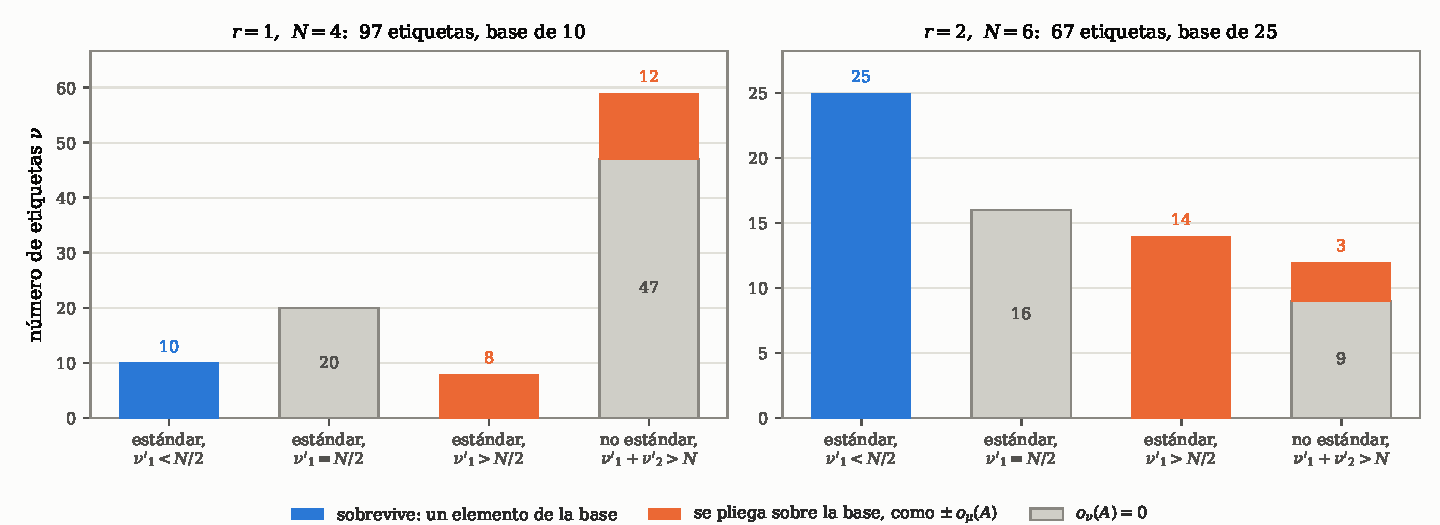
\includegraphics[width=\textwidth]{fig_reduction_es.pdf}
\caption{La reducción del Lema \ref{lem:AtoSp}, dibujada. Cada etiqueta
$\nu$ que aparece en $s_\lambda=\sum_\nu c_\nu o_\nu$ se coloca en una de cuatro clases y se calcula
su valor $o_\nu(A)$. Las etiquetas autoasociadas se anulan, todas ellas; las estándar con
$\nu'_1>N/2$ se pliegan sobre la base como $\pm o_{\mu}(A)$; las no estándar o se anulan o se pliegan
sobre un único elemento de la base con coeficiente $\pm1$. Por \eqref{eq:AtoSp} estas tres son las
reglas de modificación simplécticas disfrazadas, con las clases cortadas por $\ell(\nu)$ frente al
rango $r$; la figura se calculó antes de advertirlo y se deja tal cual. Todo aterriza en la base
independiente $\{o_\mu(A):\ell(\mu)\le r\}$, que es lo que convierte la anulación en la condición
finita \eqref{eq:Cmu}. Las alturas de las barras son recuentos de etiquetas sobre el rango en que se
calculó cada panel, menor que el de la fila correspondiente de la \S\ref{sec:verif}; lo que la imagen
cuenta es la clasificación, no el recuento.}
\label{fig:reduction}
\end{figure}
\begin{equation}\label{eq:Cmu}
\Psi_r(\lambda)=\sum_{\ell(\mu)\le r}C_\mu(\lambda)\,o_\mu(A),
\qquad
\Psi_r(\lambda)=0\iff C_\mu(\lambda)=0\ \text{para toda }\mu,
\end{equation}
donde $C_\mu=c_\mu\pm c_{\mu^{*}}+\sum\pm c_\nu$, sumando sobre las $\nu$ no estándar que se reducen
a $\mu$. La reducción se hace en dos pasos y no en uno: la mayoría de las etiquetas no estándar se
emparejan con una asociada dentro del rango, mientras que $21$ de ellas --- $18$ con $r=1$ y $3$ con
$r=2$ --- no tienen asociada en rango y se reducen aparte, cayendo cada una en el span de los valores
estándar con coeficientes enteros.

Habíamos calculado los tres hechos antes de localizarlos, y dejamos constancia del cálculo porque es
lo que dibuja la figura de abajo: \texttt{sec8\_derivation.sage} comprueba \eqref{eq:AtoSp}
directamente para todo $|\nu|\le8$, confirma que las etiquetas de longitud $r+1$ se anulan y que las
más largas se pliegan sobre la base con un signo, y verifica la independencia como un cálculo de
rango, con $r=1,2,3$. Un control que tenía que dispararse: $\iota_1 o_\nu$ y $\iota_{-1}o_\nu$
coinciden con $sp_\nu$ sólo para $\nu=\varnothing$, de modo que hacen falta las dos letras y
\eqref{eq:AtoSp} es un enunciado sobre el par recíproco y no sobre ninguna de las dos por separado.
\texttt{sec8\_formulas.sage} comprueba la demostración y no el enunciado --- la recurrencia con cuatro
valores de $c$, los dos determinantes que definen los caracteres frente a una implementación
independiente, y las operaciones de columna entrada por entrada. Esta última comprobación se ganó el
sueldo: un borrador previo de la demostración escribía $C_j\to C_j+C_{j-1}$ con $c=1$, que es el signo
que \cite[Lema 3.2]{AK25} usa para su propio paso con $c=-1$.

Las etiquetas no estándar, que son aquí toda la obstrucción, no pueden ser pequeñas:

\begin{lemma}[las etiquetas no estándar son grandes]\label{lem:nonstd}
Toda $\nu$ no estándar que aparezca en el desarrollo cumple $|\nu|\ge N+1=2r+3$. En consecuencia, si
$|\lambda|\le2r+2$ ninguna etiqueta no estándar está contenida en $\lambda$, la última suma de $C_\mu$
queda vacía y $C_\mu(\lambda)=c_\mu(\lambda)\pm c_{\mu^{*}}(\lambda)$ --- sin hipótesis alguna sobre
$\ell(\lambda)$, luego también fuera del rango de Littlewood.
\end{lemma}

\begin{proof}
Como $c^{\lambda}_{\nu\beta'}=0$ salvo si $\nu\subseteq\lambda$, solo aparecen etiquetas con
$\ell(\nu)\le\ell(\lambda)\le N$. Ser no estándar significa $\nu'_1+\nu'_2>N$. Si $\nu$ tuviera una
sola columna sería $\nu'_2=0$ y haría falta $\nu'_1=\ell(\nu)>N$, que queda excluido; luego
$\nu'_2\ge1$ y $|\nu|\ge\nu'_1+\nu'_2>N=2r+2$. Así que una $\nu$ no estándar solo puede contribuir
cuando $|\lambda|\ge|\nu|\ge2r+3$.
\end{proof}

\noindent Como $\ell(\lambda)>N/2$ obliga a $|\lambda|\ge r+2$, el Lema \ref{lem:nonstd} resuelve de
golpe la franja $r+2\le|\lambda|\le2r+2$ del rango inestable: ahí la regla de Littlewood se aplica
literalmente y el recíproco se sigue por el argumento del Teorema \ref{thm:stable}. Lo que esta ruta
todavía tiene que cruzar es $|\lambda|>2r+2$.


Dos hechos exactos acotan a los competidores. Primero, $\ell(\mu^{*})=N-\ell(\mu)$, de modo que
$\ell(\mu)\le N-1-\ell(\lambda)$ obliga a $\mu^{*}\not\subseteq\lambda$ y a $c_{\mu^{*}}=0$. Segundo,
una $\nu$ no estándar cumple $\nu'_1+\nu'_2>N$ con $\nu'_2\le\nu'_1$, luego $2\ell(\nu)>N$ y
$\ell(\nu)\ge r+2$; en particular, en el rango de Littlewood ninguna etiqueta no estándar cabe dentro
de $\lambda$. Llamemos $\mu$ \emph{aislante} para $\lambda$ si exactamente una de las etiquetas que
alimentan $C_\mu$ está contenida en $\lambda$; entonces $C_\mu=\pm c_\nu\ne0$ y
$\Psi_r(\lambda)\ne0$. Lo que la ruta pide ahí es un único enunciado de existencia ---abierto como
enunciado de existencia, aunque no como teorema, pues el Teorema \ref{conj:crit} no pasa por él---.

\begin{proposition}[el testigo aislante no siempre existe]\label{conj:iso}
En $r=2$ la forma $\lambda=(5,5,2,1)$ cumple $\Psi_2(\lambda)\ne0$ y no es de tipo {\rm(a)} ni de
tipo {\rm(b)}, y ninguna $\mu$ es aislante para ella: toda $\mu$ cuyo $C_\mu$ tenga un contribuyente
no nulo dentro de $\lambda$ tiene exactamente dos, a saber $\mu$ y su asociado $\mu^{*}$.
\end{proposition}

Habíamos propuesto el testigo aislante como la vía hacia el Teorema \ref{conj:crit}, y no llega. La
razón se lee en el lema de aislamiento: exige $\ell(\mu)\le N-1-\ell(\lambda)$, lo que con
$\ell(\lambda)=4$ y $N=6$ deja solo $\mu$ de una fila, y una forma tan ancha como $(5,5,2,1)$
contiene a todos los asociados. Sobre $r=2$ y $|\lambda|\le14$ hay once formas así, la menor esta
misma, y ninguna por debajo de $|\lambda|=13$, que es la razón de que el certificado parezca sólido
en rangos pequeños. El Teorema \ref{conj:crit} en sí queda intacto ---afirma que los $C_\mu$ se
anulan, no que exista un certificado--- pero esta vía hacia él queda cerrada. La que sí llega, la
\S\ref{sec:rigidity}, no pasa por el rango de Littlewood, y por eso el fallo de aquí cuesta la
explicación y no el teorema.

El mecanismo alcanza mucho: en $r=2$ y $|\lambda|\le14$, $227$ de las $238$ formas inestables no
nulas llevan un testigo aislante demostrado. Y alcanza más de lo que el hecho (ii) permite por sí
solo ---el mínimo real de $\ell(\nu)$ sobre las $\nu$ no estándar con $o_\nu(A)\ne0$ es allí $5$,
frente al $r+2=4$ que da la cota. Lo que lo derrota es la anchura y no la altura: la base de
\eqref{eq:Cmu} crece con $r$ y las etiquetas competidoras están obligadas a ser altas, así que
leíamos el aislamiento como algo que se facilita con $r$, y a lo largo del eje de la altura así es;
el residuo vive donde $\lambda$ es lo bastante ancha para tragarse los asociados. Esa lectura predice
dónde el residuo \emph{no} está: en $r=3$ el lema de aislamiento permite $\ell(\mu)\le7-\ell(\lambda)$,
de modo que una forma tiene que ser más ancha que en $r=2$ antes de poder tragarse todos los
asociados, y los mismos tamaños deberían salir limpios. Y salen ---sobre $r=3$ y $|\lambda|\le13$ las
$149$ formas inestables no nulas llevan todas un testigo demostrado y el residuo es vacío---, lo cual
es un control sobre la explicación, no un paso hacia el Teorema \ref{conj:crit}. En $r=1$ la
cuestión no se plantea, pues ese caso lo resuelve por separado el Teorema \ref{thm:r1}.

La herramienta a la que uno acude primero no encaja. La saturación, en la forma de panal de Knutson
y Tao \cite{KT99}, decide cuándo un coeficiente de Littlewood--Richardson aislado es positivo, y todo
competidor que alimenta a $C_\mu$ lo es en cuanto su etiqueta cabe dentro de $\lambda$. Lo que un
$\mu$ aislante pide no es positividad sino \emph{aislamiento}: que exactamente uno de ellos quepa. La
positividad es lo que vuelve difícil la pregunta, no lo que la responde, y no conocemos herramienta
alguna dirigida a la segunda.

\begin{figure}[t]
\centering
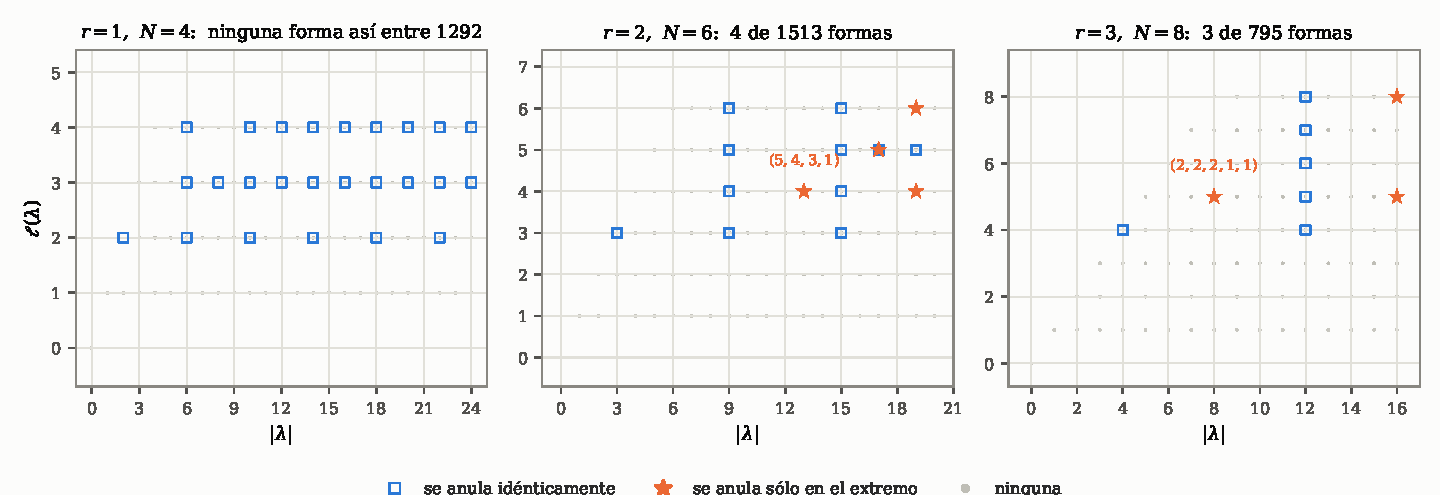
\includegraphics[width=\textwidth]{fig_phase_es.pdf}
\caption{Dónde deja de ser típico un solo par recíproco. Cada partición con a lo sumo $N$ partes es un
punto en $(|\lambda|,\ell(\lambda))$; la clase dibujada con estrella es la que se anula en el extremo
$z_i=1$ sin anularse idénticamente, y es todo el contenido de la imagen; cada panel nombra a su
miembro más pequeño y la Observación \ref{rem:rankone} enumera los demás.
Los paneles cubren $|\lambda|\le24$, $20$ y $16$ respectivamente. En $r=1$ la clase
está vacía sobre las $1292$ formas del rango, porque allí el objeto es $\pm$ un carácter genuino y su
valor en la identidad es una dimensión. A partir de $r=2$ aparecen ejemplos genuinamente virtuales y
la clase deja de estar vacía ---no que toda forma lo sea: el Cuadro \ref{tab:virtual} cuenta las dos
cosas---. Véase la Observación \ref{rem:rankone}.}
\label{fig:phase}
\end{figure}

\begin{remark}[el accidente de rango uno, y dónde se separan los dos rangos]\label{rem:rankone}
En $r=1$ el objeto es $\pm$ un carácter genuino, así que su valor en la identidad es una dimensión y
$\Psi_1(\lambda)\equiv0$ si y solo si $\Psi_1(\lambda)|_{z=1}=0$. En $r\ge2$ la expansión plegada
\emph{puede} ser genuinamente virtual ---no que lo sea siempre, y el Cuadro \ref{tab:virtual} cuenta
las dos columnas---, y basta una forma en que lo sea para romper esa equivalencia:
$\lambda=(5,4,3,1)$ con $r=2$ cumple
$\Psi_2(\lambda)\ne0$ y $\Psi_2(\lambda)|_{z_1=z_2=1}=0$. La Figura \ref{fig:virtual} muestra
los dos regímenes uno al lado del otro, sobre dos formas que difieren en una sola casilla. Sobre los rangos de la Figura
\ref{fig:phase}, la clase de tales formas está vacía en $r=1$ a lo largo de $1292$ particiones; en
$r=2$ consta de las cuatro formas $(5,4,3,1)$, $(5,5,4,2,1)$, $(10,5,3,1)$ y $(6,5,4,2,1,1)$, y en
$r=3$ de las tres formas $(2,2,2,1,1)$, $(5,5,4,1,1)$ y $(3,3,3,2,2,1,1,1)$; es delgada, pero no está
vacía, y un solo contraejemplo es todo lo que la equivalencia puede soportar. La implicación que sí
sobrevive ---anulación exacta $\Rightarrow$ anulación en el extremo--- es lo que hace del extremo un
tamiz válido y nada más. Por eso los resultados calculados en elementos de orden dos ---Karmakar
\cite{Kar24} a lo largo de toda esa familia, Eisenkölbl \cite{Eis07} en el equilibrado
$x_i=(-1)^i$--- hablan de un punto y no de la curva, y por eso el
Teorema \ref{thm:zeros} no es un corolario suyo para $r\ge2$.
\end{remark}

Conviene ponerle un número a lo que el tamiz del extremo deja escapar, porque el enunciado
cualitativo se lee con facilidad como una corrección pequeña. Sobre los rangos de la Figura
\ref{fig:phase}, el contraste $\Psi_r(\lambda)|_{z_i=1}=0$ señala $143$ formas en $r=1$, $22$ en $r=2$
y $9$ en $r=3$; de ellas, $0$, $4$ y $3$ respectivamente no se anulan idénticamente. El tamiz es
entonces exacto con un solo par, y la proporción de sus veredictos que resultan espurios crece con el
número de pares: $0\%$, $18\%$, $33\%$ sobre estos rangos. Un cálculo en el extremo es un filtro que
nunca se salta un cero genuino, y pasado un par no es nada más que eso. El caso de rango uno con
$t=2$, donde el tamiz resulta exacto porque el objeto es un carácter genuino, se trató aparte en
\cite{Mar26}; el alfabeto \eqref{eq:object} surgió allí, en un cálculo de líneas de Wilson sobre un
orbifold, y de ahí que el $-1$ aparezca como letra y no como elección.

Vale la pena separar la razón de que los dos rangos de $\ell(\lambda)$ se comporten de forma tan
distinta del mecanismo que lo demuestra. La regla de Littlewood dice qué etiquetas $\nu$ pueden
aparecer, y $\ell(\lambda)\le N/2$ es exactamente la condición bajo la cual las no estándar no caben
dentro de $\lambda$. El Lema \ref{lem:nonstd} dice que la obstrucción la gobierna $|\lambda|$ además
de $\ell(\lambda)$, así que la imagen honesta no es de dos rangos sino de una región: \emph{esta
ruta} alcanza el recíproco allí donde $\ell(\lambda)\le N/2$ o bien $|\lambda|\le2r+2$, y fuera de la
unión de ambas no llega ---el testigo aislante cubre casi todo lo que queda pero demostrablemente no
todo, por la Proposición \ref{conj:iso}---. El recíproco no está abierto ahí. El Teorema
\ref{conj:crit} lo resuelve para todo $r$ y toda $\lambda$ por el argumento extremal de las
\S\S\ref{sec:extremal}--\ref{sec:rigidity}, que no entra en este rango en absoluto. Lo que la región
marca es dónde deja de explicar la reducción de Littlewood, no dónde deja de valer el teorema.

%======================================================================
% ---- v2_new_subsections_es.tex ----
\subsection{El criterio en \texorpdfstring{$t=2$}{t=2}: el argumento extremal}\label{sec:extremal}

En esta subsección y en las dos siguientes, $t\ge2$ y $r\ge1$ son arbitrarios y
\[
  N:=t+2r,\qquad
  \Phi_{t,r}(\lambda;z):=s_\lambda\bigl(\zt,\,z_1,\zb_1,\dots,z_r,\zb_r\bigr),
\]
de modo que $\Phi_{t,1}$ es \eqref{eq:object} y $\Phi_{2,r}=\Psi_r$. El beta-conjunto, los recuentos
de residuos $n_i$ y la indexación de las columnas son los de la \S\ref{sec:background}; $\lambda\in\PP_N$ y
$\beta_1>\dots>\beta_N\ge0$. Escribimos
\[
  \mathcal{E}=\{i:n_i(\lambda)\ge2\},\qquad e=|\mathcal{E}|,\qquad
  \mathcal{S}=\{\beta_j:\beta_j\equiv i\ (t)\ \text{para algún } i\in\mathcal{E}\}
\]
para las \emph{clases de exceso} y los \emph{valores de exceso}. Como las $t-e$ clases restantes son
unitarias, \eqref{eq:excess} se convierte en
\begin{equation}\label{eq:excessgen}
  \sum_{i\in\mathcal{E}}\bigl(n_i(\lambda)-1\bigr)=2r,\qquad |\mathcal{S}|=2r+e,\qquad 1\le e\le2r .
\end{equation}
Suponemos siempre la \emph{hipótesis de ocupación} $n_i\ge1$ para todo $i$; por el Lema
\ref{lem:L1} su fallo da $\Phi_{t,r}\equiv0$ de entrada, que es la rama (a).

\begin{lemma}[la descomposición de Laplace, $r$ general]\label{lem:L3gen}
Sea $\mathcal T$ el conjunto de los $t$-subconjuntos $S$ de columnas que llevan los $t$ residuos, y
para $S\in\mathcal T$ sea $A(S^{c})$ el menor de $\det(x_i^{\beta_j})$ sobre las $2r$ filas que
llevan $z_1,\zb_1,\dots,z_r,\zb_r$ y las columnas $S^{c}$. Entonces
\begin{equation}\label{eq:laplacegen}
  \det\bigl(x_i^{\beta_j}\bigr)_{i,j=1}^{N}
  \;=\;(-1)^{\binom{t+1}{2}}\,V\sum_{S\in\mathcal T}w(S)\,A(S^{c}),
  \qquad
  w(S)=(-1)^{\,\sum_{j\in S}j+\inv(b_S)} .
\end{equation}
\end{lemma}

\begin{proof}
Laplace por las $t$ primeras filas da
\[
\det(x_i^{\beta_j})=\sum_{|S|=t}(-1)^{\binom{t+1}{2}+\sum_{j\in S}j}M_S\,A(S^{c}).
\]
Por el Lema
\ref{lem:L1}, $M_S=0$ salvo que los residuos $b_S$ sean distintos dos a dos --- es decir, salvo que
$S\in\mathcal T$ --- y entonces $M_S=(-1)^{\inv(b_S)}V$.
\end{proof}

En $r=1$ el menor complementario es el determinante $2\times2$ igual a $f(\beta_{j_1}-\beta_{j_2})$ y
\eqref{eq:laplacegen} es el Lema \ref{lem:L3}; lo que sigue es lo que sustituye a ese menor
$2\times2$ cuando $r>1$. Sólo importan los signos relativos $w(S)$ y, como un elemento de
$\mathcal T$ queda determinado por qué valor de exceso conserva en cada clase de exceso --- las
clases unitarias las conserva todo $S$ ---, indexamos los términos por esa elección, escrita $g$, y
ponemos $T_g=\mathcal{S}\setminus g$, un conjunto de $2r$ valores escritos en orden decreciente.

Conviene resolver aquí una pregunta, porque todo lo que sigue mueve $g$ de un lado a otro y hay que
llevarse el signo consigo: qué le pasa a $w$ cuando cambia la elección en una sola clase. En $r=1$
eso es el Lema \ref{lem:L4}, donde una clase tiene dos elementos y no hay nada entre medias. En
general sí lo hay.

\begin{lemma}[el movimiento de columna, con clases de cualquier tamaño]\label{lem:step}
Sean $g$ y $g'$ coincidentes fuera de una clase, y elijan en ella los valores $u>v$ respectivamente.
Entonces
\begin{equation}\label{eq:step}
\frac{w(g')}{w(g)}\;=\;(-1)^{\,1+B+M},
\end{equation}
donde $B=\#\{\beta_j:v<\beta_j<u\}$ y $M$ es el número de valores \emph{congelados} que quedan
estrictamente entre $v$ y $u$ ---los $t$ valores que una transversal conserva, uno en cada clase de
residuos, o sea los $e$ valores de $g$ junto con las $t-e$ clases singleton---. Puede contarse en $g$
o en $g'$ indistintamente, pues coinciden estrictamente entre $v$ y $u$.
\end{lemma}

\begin{proof}
Los dos conjuntos congelados difieren en sustituir la columna de $u$ por la de $v$. Como $\beta$ es
estrictamente decreciente, ese índice de columna aumenta en $B+1$, que es la variación de
$\sum_{j\in S}j$. En la palabra $b_S$ la letra que lleva esa columna se desplaza por delante de
exactamente las $M$ letras congeladas que quedan estrictamente en medio, y cada cruce cambia $\inv$
en uno; la letra en sí no cambia, y las $B-M$ columnas intermedias que \emph{no} están congeladas no
aportan ninguna letra. Así que $\inv(b_S)$ varía en $M$ módulo $2$, y \eqref{eq:step} se sigue de la
definición de $w$ en el Lema \ref{lem:L3gen}.
\end{proof}

\noindent El Lema \ref{lem:L4} es el caso $B=M=0$ de éste, leído dos veces. La contabilidad es la
misma que Albion \cite{Alb23,Alb25} y Ayyer--Behrend \cite{AB19} hacen cada vez que mueven o invierten
un bloque de columnas y recogen el signo, y la seguimos porque es la que este tipo de determinante
pide; la escribimos en esta forma sólo porque la \S\ref{sec:rigidity} mueve una columna muchas veces
y la cuenta tiene entonces que ser exacta y no absorbida en una constante. Los dos términos tienen
que estar los dos: quitar cualquiera de ellos da una regla que acierta aproximadamente la mitad de
las veces, y $B-M$ es exactamente el número de columnas intermedias que ninguna transversal congela
---por lo cual una clase de tamaño dos, sin nada entre sus elementos, esconde la distinción---. Las
clases singleton hay que contarlas también en $M$, y no es una formalidad: leer $M$ sólo sobre las
elecciones $g$ ya falla en $t=3$, $r=1$ con $\beta=(4,3,2,1,0)$, donde mover la clase del $1$ de
$u=4$ a $v=1$ da $B=2$ y un valor congelado intermedio que vive en una clase singleton, de modo que
las dos lecturas difieren en un signo.

\subsubsection*{La filtración por grados}

Para un monomio $\prod_j z_j^{c_j}$ usamos el \emph{grado total} $\sum_j c_j$. Todo monomio de
$A(S^{c})$ tiene la forma $\prod_j z_j^{\,u-u'}$ para un emparejamiento de $T_g$ en pares ordenados
asignados a las variables, así que, escribiendo $T=(u_1>\dots>u_{2r})$,
\begin{equation}\label{eq:deggen}
  \deg(T):=\sum_{a\le r}u_a-\sum_{a>r}u_a
\end{equation}
es el mayor grado total que aparece en $A$, alcanzado exactamente por los emparejamientos que unen la
mitad de arriba $H=(u_1,\dots,u_r)$ con la de abajo $L=(u_{r+1},\dots,u_{2r})$. Escribiendo
$a_X(z)=\det(z_j^{X_i})_{r\times r}$ y $P(T)=a_H(z)a_L(z^{-1})$, que no es nulo por ser producto de
dos alternantes de $GL(r)$, la componente de grado total máximo de $A$ es
\begin{equation}\label{eq:Amaxgen}
  [A]_{\deg(T)}\;=\;(-1)^{\binom r2}\,P(T).
\end{equation}
En efecto, en grado máximo cada variable recibe una fila de $H$ con exponente positivo y una de $L$
con exponente negativo, y las dos asignaciones son independientes, así que la suma se factoriza en
los dos determinantes; el signo es el de la permutación que reparte las filas de $H$ entre las
columnas $z_1,\dots,z_r$ y las de $L$ entre las columnas $z_1^{-1},\dots,z_r^{-1}$, intercalándolas,
y vale $(-1)^{\binom r2}$.
Bajo la graduación por $\sum_j|c_j|$ la componente máxima se parte en $2^r$ sectores de orientación
con monomios disjuntos, permutados por $z_j\mapsto z_j^{-1}$ con un signo uniforme, así que se anulan
a la vez; todos los enunciados de abajo usan el grado total.

\begin{lemma}[reflexión]\label{lem:reflgen}
$P(c-T)=P(T)$ para todo $c\in\ZZ$ y todo $T$.
\end{lemma}

\begin{proof}
La mitad de arriba de $c-T$ es $c-L$ listada en orden decreciente, así que
$a_{c-L}(z)=(\prod_j z_j^{c})(-1)^{\binom r2}a_L(z^{-1})$, y simétricamente para la mitad de abajo.
Las dos potencias de $\prod_j z_j^{c}$ se cancelan y $(-1)^{r(r-1)}=+1$.
\end{proof}

Sea $G$ el conjunto de las $g$ que maximizan $\deg(T_g)$ y $D_1$ ese máximo. Como el numerador
$\det(x_i^{\beta_j})$ y $\Phi_{t,r}$ difieren en el factor no nulo $\det(x_i^{N-j})$, se tiene
$\Phi_{t,r}\equiv0$ si y sólo si el numerador se anula, y \emph{todo grado y todo estrato de aquí en
adelante se refieren al numerador}; no se compara ninguna de sus partes homogéneas con las del
cociente. Por \eqref{eq:laplacegen},
\begin{equation}\label{eq:topgen}
  \bigl[\det(x_i^{\beta_j})\bigr]_{D_1}
  =(-1)^{\binom{t+1}{2}+\binom r2}\,V\sum_{g\in G}w(g)\,P(T_g),
\end{equation}
donde el segundo signo viene de \eqref{eq:Amaxgen}. Abajo sólo importan los signos relativos $w(g)$,
así que la constante global se anota una vez y no se arrastra.

\begin{remark}[un aviso sobre ese signo global]
Es tentador suprimir $(-1)^{\binom r2}$ con el argumento de que nada de lo que sigue depende de él, y
lo anotamos por la razón contraria: una identidad enunciada es una identidad que se comprueba, y ésta
es \emph{falsa} sin él en cuanto $r\ge2$. El signo no es adorno. Es la signatura de la permutación
intercalada de \eqref{eq:Amaxgen} --- $+1$ para $r=1$ y para $r\equiv0,1 \pmod 4$, $-1$ en los demás
casos --- y es
invisible en $r=1$, que es justo el rango en el que uno escribe la fórmula por primera vez.
\end{remark}

% ---- v2_block2_es.tex ----
\subsubsection*{El conjunto extremal tiene a lo sumo dos elementos}

Para $i\in\mathcal{E}$ listamos los valores de exceso de la clase en orden decreciente,
$c_{i,1}>c_{i,2}>\dots>c_{i,n_i}$ con $n_i=n_i(\lambda)$, y definimos sus \emph{incrementos}
\begin{equation}\label{eq:incrgen}
  \Delta_i(k)\;:=\;c_{i,k}+c_{i,k+1},\qquad 1\le k\le n_i-1 .
\end{equation}
Por \eqref{eq:excessgen} hay exactamente $2r$ en total; escribimos
$\Delta_{(1)}\ge\dots\ge\Delta_{(2r)}$ para la lista en orden decreciente y ponemos
$\tau:=\Delta_{(r)}$.

\begin{theorem}[el conjunto extremal]\label{thm:Ggen}
Supóngase $n_i\ge1$ para todo $i$. Entonces
\begin{enumerate}
\item[\rm(a)] $g\in G$ si y sólo si el multiconjunto de incrementos que selecciona, en el sentido del
Paso 2 de abajo, consta de todos los incrementos $>\tau$ junto con suficientes incrementos iguales a
$\tau$;
\item[\rm(b)] $|G|\le2$, y $|G|=2$ si y sólo si $\Delta_{(r)}=\Delta_{(r+1)}$, en cuyo caso $t$ es
par, los dos incrementos empatados pertenecen a las clases $i$ e $i+t/2$ --- ambas necesariamente en
$\mathcal{E}$ --- y los dos maximizadores difieren exactamente en esas dos clases;
\item[\rm(c)] si $t$ es impar entonces $|G|=1$.
\end{enumerate}
\end{theorem}

\begin{proof}
\emph{Paso 1 (reformulación).} Para todo $2r$-conjunto $T$,
\[
\deg(T)=\max_{A\subseteq T,\,|A|=r}\bigl(2\Sigma A-\Sigma T\bigr),
\]
con el máximo alcanzado en la mitad de arriba. Con $T=\mathcal{S}\setminus g$ esto se lee
$\deg(\mathcal{S}\setminus g)=\max_A\bigl[2\Sigma A+\Sigma g\bigr]-\Sigma\mathcal{S}$, de modo que
maximizamos $\Theta(A,g)=2\Sigma A+\Sigma g$ sobre pares disjuntos con $|A|=r$ y $g$ una elección de
un valor de exceso en cada clase de exceso.

\emph{Paso 2 (forma de un óptimo).} Sea $(A,g)$ óptimo y sean $x>y$ de la misma clase $i$. Si $y\in A$
y $x=g_i$, intercambiarlos deja $g$ admisible y cambia $\Theta$ en $x-y>0$; si $y=g_i$ y $x$ no está
ni en $A$ ni en $g$, el mismo intercambio da $x-y>0$. Ambos son imposibles, así que dentro de cada
clase, leída en orden decreciente, van primero los elementos de $A$, luego $g_i$, y luego los no
elegidos. Por tanto un óptimo queda parametrizado por un entero por clase,
$k_i=|A\cap\text{clase }i|\in\{0,\dots,n_i-1\}$ con $\sum_i k_i=r$, mediante
$A\cap\text{clase }i=\{c_{i,1},\dots,c_{i,k_i}\}$ y $g_i=c_{i,k_i+1}$. La aplicación $(k_i)\mapsto g$
es inyectiva y, fijado $g$, el $A$ óptimo es la mitad de arriba de $T_g$, así que los pares óptimos se
proyectan biyectivamente sobre $G$.

\emph{Paso 3 (separabilidad).} Con esa parametrización $\Theta=\sum_{i\in\mathcal{E}}f_i(k_i)$, con
$f_i(k)=2(c_{i,1}+\dots+c_{i,k})+c_{i,k+1}$: el objetivo se parte sobre las clases y el único
acoplamiento es $\sum_i k_i=r$.

\emph{Paso 4 (el intercambio).} $f_i(k)-f_i(k-1)=\Delta_i(k)$, estrictamente decreciente en $k$
porque los $c_{i,k}$ lo son, luego
\[
\Theta=\sum_{i\in\mathcal{E}}f_i(0)+\Sigma,\qquad
\Sigma=\sum_{i\in\mathcal{E}}\sum_{k\le k_i}\Delta_i(k),
\]
y maximizar $\Theta$ es maximizar $\Sigma$. Un $(k_i)$ factible selecciona, en cada clase, un
\emph{prefijo} de la lista de incrementos de esa clase, con $r$ incrementos en total; llamemos
\emph{admisible} a una selección así. Tómese ahora cualquier conjunto de $r$ incrementos de suma
máxima, sea admisible o no. Esa selección \emph{es} admisible: si contuviera $\Delta_i(k)$ sin
$\Delta_i(k-1)$, intercambiar los dos subiría la suma, porque $\Delta_i(k-1)>\Delta_i(k)$ ---y el
intercambio es legítimo porque $\Delta_i(k-1)$ no estaba ya seleccionado---. Y ninguna selección
admisible puede superar la suma de los $r$ incrementos mayores, siendo ella misma una selección de
$r$ de ellos. Luego los maximizadores de $\Theta$ son exactamente las selecciones admisibles cuyo
multiconjunto de incrementos es un multiconjunto de $r$ mayores, que es lo que afirma {\rm(a)}.
(Es el algoritmo voraz de asignación marginal para un objetivo separable cóncavo bajo una
restricción de cardinal; véanse \cite{FG86,IK88}. Damos el argumento porque son cuatro líneas, de
modo que el Teorema \ref{conj:crit} no se apoye en más resultado ajeno que el Teorema
\ref{thm:PvW}.)

\emph{Paso 5 (residuos).} $c_{i,k}\equiv c_{i,k+1}\equiv i$, luego
\begin{equation}\label{eq:congrgen}
  \Delta_i(k)\;\equiv\;2i \pmod t .
\end{equation}
Dentro de una clase los incrementos son distintos dos a dos por el Paso 4. Entre clases,
$\Delta_i(k)=\Delta_{i'}(k')$ fuerza $2i\equiv2i'$, es decir $i'=i$ o --- sólo si $t$ es par ---
$i'=i+t/2$. Por tanto \emph{ningún valor lo comparten más de dos incrementos}, y cuando lo comparten,
los dos vienen de las clases $i$ e $i+t/2$.

\emph{Paso 6.} Los óptimos son las selecciones que contienen todo incremento $>\tau$ junto con $s$ de
los iguales a $\tau$, con $s\ge1$. A lo sumo dos incrementos valen $\tau$, así que o caben los dos
($|G|=1$) o cabe exactamente uno ($|G|=2$), esto último precisamente cuando
$\Delta_{(r)}=\Delta_{(r+1)}$. Para $t$ impar, $x\mapsto2x$ es inyectiva en $\ZZ/t$, así que no hay
empate posible y $|G|=1$.
\end{proof}

\begin{remark}
El contenido del Teorema \ref{thm:Ggen} es \eqref{eq:congrgen} junto con el hecho de que
$x\mapsto2x$ en $\ZZ/t$ tiene núcleo de orden $\gcd(2,t)$: la multiplicidad de un valor extremal la
controla la $2$-torsión del grupo de residuos, que es la razón de que la paridad de $t$ lo gobierne
todo aquí y en la \S\ref{sec:main}. Los Pasos 1--4 sólo usan que los $\beta_j$ sean enteros
distintos; ni $\beta_j\ge0$, ni que $\lambda$ sea una partición, ni $N=t+2r$ intervienen más allá de
\eqref{eq:excessgen}. La Figura \ref{fig:increments} es el teorema hecho sobre una forma concreta,
con el empate y la forma de prefijo del Paso 2 a la vista.
\end{remark}

\begin{remark}[de dónde viene esta forma de argumento]
Los Pasos 1--4 son una historia vieja contada en otro alfabeto. Maximizar un objetivo separable
cóncavo bajo una restricción de cardinal es el problema clásico de asignación marginal de recursos,
que resuelve el algoritmo voraz \cite{FG86,IK88}; hemos dado el intercambio en cuatro líneas sólo para
que el lector no tenga que salir del artículo. El Paso 6 también es conocido, aunque venga de otra
tradición: en álgebra lineal tropical la forma inicial de un determinante es la suma con signo sobre
las asignaciones \emph{óptimas}, y la matriz se llama tropicalmente singular exactamente cuando dos o
más óptimos alcanzan el óptimo \cite{TropCramer}. Leída así, \eqref{eq:topgen} dice que nuestro
numerador es tropicalmente singular precisamente cuando $|G|=2$, y toda la cuestión de la
\S\ref{sec:rigidity} es si los dos óptimos se cancelan. Lo que \emph{no} es estándar, y es la razón de
que la paridad de $t$ lo gobierne todo, es \eqref{eq:congrgen}: es una congruencia, no una
desigualdad, y es lo que acota por dos el número de óptimos.
\end{remark}

\begin{figure}[!ht]
\centering
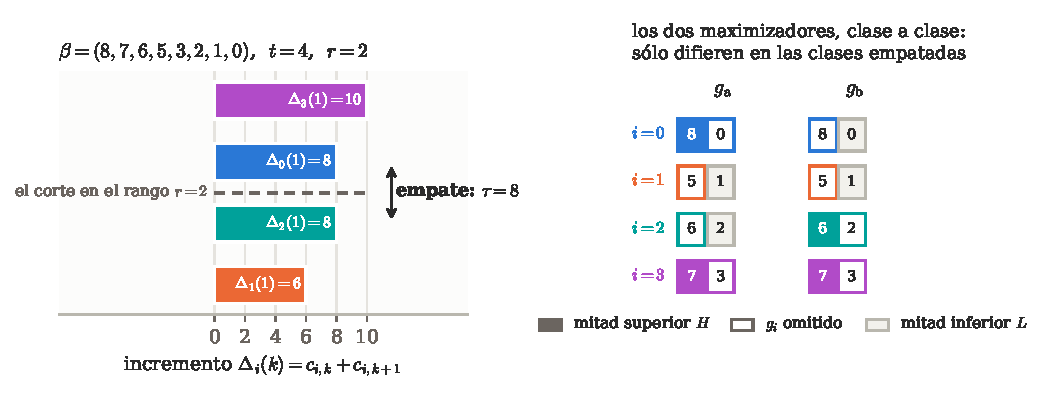
\includegraphics[width=\textwidth]{fig_increments_es.pdf}
\caption{El Teorema \ref{thm:Ggen} hecho sobre una forma, en vez de enunciado. Para
$\beta=(8,7,6,5,3,2,1,0)$ con $t=4$, $r=2$ las cuatro clases de exceso son $\{8,0\}$, $\{5,1\}$,
$\{6,2\}$, $\{7,3\}$ y los cuatro incrementos son $\Delta_3(1)=10$, $\Delta_0(1)=8$,
$\Delta_2(1)=8$, $\Delta_1(1)=6$. Un maximizador toma los $r=2$ mayores; el segundo y el tercero son
iguales, así que $\tau=\Delta_{(2)}=\Delta_{(3)}=8$ y hay exactamente dos. La pareja empatada
pertenece a las clases $0$ y $2=0+t/2$, que es \eqref{eq:congrgen} y no una casualidad: ningún valor
lo comparten incrementos de clases distintas de $i$ e $i+t/2$. A la derecha los dos maximizadores
están dibujados clase a clase en la forma de prefijo del Paso 2 --- leyendo una clase en orden
decreciente, primero los elementos de la mitad de arriba, luego el omitido $g_i$, luego los de la
mitad de abajo ---, lo que hace visible que difieren en las clases empatadas y en ninguna otra. El
color codifica la clase, no el rango. Calculada por \texttt{anc/fig\_v2.py}.}
\label{fig:increments}
\end{figure}

\begin{corollary}[un maximizador único]\label{cor:uniquegen}
Si $|G|=1$ entonces $\Phi_{t,r}\not\equiv0$.
\end{corollary}

\begin{proof}
Por \eqref{eq:topgen} la componente del numerador en grado $D_1$ es $\pm V\,P(T_g)\ne0$ para el único
$g$. Un polinomio de Laurent con una componente homogénea no nula no es nulo, así que el numerador no
es nulo y por tanto tampoco lo es $\Phi_{t,r}$.
\end{proof}

\begin{corollary}[el bloque central]\label{cor:midgen}
Escríbase $\mathcal{S}=\{s_1>\dots>s_n\}$, $n=2r+e$. Si el bloque $\{s_{r+1},\dots,s_{r+e}\}$
contiene exactamente un elemento de cada clase de exceso, entonces $\Phi_{t,r}\not\equiv0$.
\end{corollary}

\begin{proof}
$\deg(\mathcal{S}\setminus g)\le(s_1+\dots+s_r)-(s_{n-r+1}+\dots+s_n)$, porque los $r$ elementos
mayores de $\mathcal{S}\setminus g$ están dominados término a término por $s_1,\dots,s_r$ y sus $r$
menores dominan a $s_{n-r+1},\dots,s_n$. La igualdad obliga a que $\mathcal{S}\setminus g$ contenga
los dos bloques extremos, es decir $g\subseteq\{s_{r+1},\dots,s_{r+e}\}$, y $|g|=e$ fuerza la igualdad
de los dos conjuntos. Así que la cota la alcanza exactamente un término y se aplica el Corolario
\ref{cor:uniquegen}.
\end{proof}

\begin{corollary}[$t$ impar]\label{cor:oddgen}
Sea $t$ impar y $r\ge1$. Entonces $\Phi_{t,r}(\lambda;z)\equiv0$ si y sólo si alguna clase de residuos
módulo $t$ está ausente de $\beta(\lambda)$.
\end{corollary}

\begin{proof}
Si algún $n_i=0$ entonces $\mathcal T=\varnothing$ en el Lema \ref{lem:L3gen} y el numerador se anula.
Recíprocamente, si todos los $n_i\ge1$ entonces $|G|=1$ por el Teorema \ref{thm:Ggen}(c) y se aplica
el Corolario \ref{cor:uniquegen}.
\end{proof}

\begin{remark}
Para $r=1$ el Corolario \ref{cor:oddgen} es la Proposición \ref{rem:lattice}, demostrada allí viendo
que la cláusula concéntrica es vacua para $t$ impar --- un argumento interno al perfil de dos clases
que fuerza un solo par recíproco. Lo nuevo es que el enunciado sobrevive para todo $r\ge1$, y por una
ruta que no menciona el perfil en absoluto: la congruencia \eqref{eq:congrgen}. En $r=0$ es falso,
puesto que la regla de Littlewood da $s_\lambda(\zt)=0$ siempre que el $t$-núcleo es no vacío, $t$
impar incluido; y la observación de que $\prod\zt=+1$ para $t$ impar no lo entrega por sí sola,
porque el alfabeto es un subtoro de dimensión $r$ con las coordenadas restantes congeladas.
\end{remark}

% ---- v2_block3_es.tex ----
\subsection{El criterio en \texorpdfstring{$t=2$}{t=2}: rigidez y reflexión}\label{sec:rigidity}

El Corolario \ref{cor:uniquegen} resuelve toda forma con un maximizador único. Lo que sigue es la
otra mitad: cuando $|G|=2$, los dos términos de \eqref{eq:topgen} sólo pueden cancelarse si las dos
transversales son reflexión una de otra, y esa rigidez la aporta un único resultado ajeno.

\begin{theorem}[Purbhoo--van Willigenburg {\cite[Thm.~2.5]{PvW}}]\label{thm:PvW}
Para particiones con a lo sumo $n$ partes, escribiendo $\lambda^{-}:=\lambda/(\lambda_n)^{n}$,
\[
  s_\lambda(x_1,\dots,x_n)\,s_\mu(x_1,\dots,x_n)=s_\nu(x_1,\dots,x_n)\,s_\rho(x_1,\dots,x_n)
\]
si y sólo si $\lambda_n+\mu_n=\nu_n+\rho_n$ y $\{\lambda^{-},\mu^{-}\}=\{\nu^{-},\rho^{-}\}$ como
multiconjuntos.
\end{theorem}

\begin{remark}
El Teorema 3 de \cite{Rajan} da el enunciado para $n$ factores, pero bajo la hipótesis de que todos
los pesos máximos sean no nulos. El Teorema \ref{thm:PvW} no necesita tal hipótesis, y por eso es el
que usamos aquí: el caso degenerado, un factor trivial, es exactamente lo que produce el Lema
\ref{lem:dictgen} siempre que $\alpha^{*}$ o $\tilde\alpha$ es vacía. Ninguno de los dos enunciados
puede atajarse por factorización única, ya que los polinomios de Schur no son irreducibles:
$s_{(3)}(x,y)=(x+y)(x^2+y^2)$.
\end{remark}

\subsubsection*{El diccionario}

Escríbase $T=(u_1>\dots>u_{2r})$ con mitades $H=(h_1>\dots>h_r)$ y $L=(l_1>\dots>l_r)$, sea
$\delta=(r-1,r-2,\dots,0)$, de modo que $a_\delta(z)=\det(z_j^{\,r-i})$ es el determinante de
Vandermonde en la notación de la \S\ref{sec:extremal}, y póngase
\[
  \alpha=H-\delta,\qquad \tilde\alpha=\alpha-(\alpha_r)^{r},\qquad
  L^{*}=(l_1-l_r>\dots>l_1-l_1),\qquad \alpha^{*}=L^{*}-\delta .
\]

\begin{lemma}[el diccionario]\label{lem:dictgen}
$\alpha^{*}_r=0$ y
\begin{equation}\label{eq:dictgen}
  P(T)\;=\;(-1)^{\binom r2}\Bigl(\textstyle\prod_j z_j\Bigr)^{h_r-l_1}
  a_\delta(z)^2\,s_{\tilde\alpha}(z)\,s_{\alpha^{*}}(z).
\end{equation}
En particular $P$ no cambia bajo $T\mapsto T+m$ ni, por el Lema \ref{lem:reflgen}, bajo
$T\mapsto c-T$.
\end{lemma}

\begin{proof}
$a_H(z)=s_\alpha(z)a_\delta(z)$ es la fórmula bialternante. Para el segundo factor, multiplicar la
columna $j$ de $\det(z_j^{-l_i})$ por $z_j^{l_1}$ da
$(\prod_j z_j^{l_1})a_L(z^{-1})=\det(z_j^{\,l_1-l_i})$, cuyos exponentes de fila crecen con $i$;
invertir las $r$ filas cuesta $(-1)^{\binom r2}$ y produce $a_{L^{*}}(z)=s_{\alpha^{*}}(z)a_\delta(z)$.
Finalmente $s_\alpha=(\prod_j z_j)^{\alpha_r}s_{\tilde\alpha}$ y $\alpha_r=h_r$.
\end{proof}

\begin{proposition}[la órbita de $P$]\label{prop:orbitgen}
Sean $T,\widetilde T$ conjuntos de $2r$ enteros distintos con $P(T)=\pm P(\widetilde T)$. Entonces
$\widetilde T=T+m$ para algún $m\in\ZZ$, o bien $\widetilde T=c-T$ para algún $c\in\ZZ$.
\end{proposition}

\begin{proof}
Dos observaciones primero. El signo es $+$: por \eqref{eq:dictgen} los dos lados son un monomio por
$a_\delta^2$ por un producto de dos polinomios de Schur, que tiene coeficientes no negativos, así que
un signo menos es imposible. Y el monomio hay que reabsorberlo: con $d=h_r-l_1\ge1$, lo que se cumple
porque $T$ es estrictamente decreciente, $(\prod_j z_j)^{d}s_{\tilde\alpha}=s_{\tilde\alpha+(d^{r})}$,
y es ese $d$ el que hace el papel de $\lambda_n+\mu_n$ en el Teorema \ref{thm:PvW}, estando
$\alpha^{*}$ ya normalizada. Cancelando $a_\delta^2$ y aplicando el Teorema \ref{thm:PvW} con $n=r$ a
$(\lambda,\mu)=(\tilde\alpha+(d^{r}),\alpha^{*})$ y al par correspondiente $(\nu,\rho)$ de
$\widetilde T$, el criterio dice que el entero $d$ coincide y que $\{\tilde\alpha,\alpha^{*}\}$
coincide como multiconjunto. Coincidir en el mismo orden dice que $H,\widetilde H$ y $L,\widetilde L$
son trasladados, y la igualdad de los dos enteros $d$ fuerza la misma traslación en las dos mitades,
es decir $\widetilde T=T+m$. Coincidir tras intercambiar dice que $H$ es, salvo traslación, la
inversa de $\widetilde L$ y $L$ la de $\widetilde H$, es decir $\widetilde T=c-T$.
\end{proof}

\subsubsection*{Los dos maximizadores se reflejan}

De aquí al final de la subsección supóngase $|G|=2$ y escríbase
$G=\{g_{\mathrm a},g_{\mathrm b}\}$, $T_{\mathrm a}=\mathcal{S}\setminus g_{\mathrm a}$,
$T_{\mathrm b}=\mathcal{S}\setminus g_{\mathrm b}$, con mitades
$T_{\mathrm a}=H_{\mathrm a}\sqcup L_{\mathrm a}$ y $T_{\mathrm b}=H_{\mathrm b}\sqcup L_{\mathrm b}$,
y
\[
  \mathcal{K}=T_{\mathrm a}\cap T_{\mathrm b}.
\]
Por el Teorema \ref{thm:Ggen}(b) las dos transversales difieren exactamente en las clases empatadas
$i$ e $i'=i+t/2$, digamos
\begin{equation}\label{eq:swapgen}
  g_{\mathrm a}\ni p_1=c_{i,k+1},\ q_1=c_{i',k'},\qquad
  g_{\mathrm b}\ni p_2=c_{i,k},\ q_2=c_{i',k'+1},
\end{equation}
de modo que $p_1+p_2=q_1+q_2=\tau$ por \eqref{eq:incrgen}: el valor del empate es la suma de cada
pareja intercambiada.

\begin{proposition}[la traslación fuerza la reflexión]\label{prop:translgen}
Si $T_{\mathrm b}=T_{\mathrm a}+m$ con $m\ne0$, entonces $T_{\mathrm b}=\tau-T_{\mathrm a}$.
\end{proposition}

\begin{proof}
$|T_{\mathrm a}\cap(T_{\mathrm a}+m)|=|\mathcal{K}|=2r-2$. Póngase una arista $x\to x+m$ cuando $x$ y
$x+m$ estén los dos en $T_{\mathrm a}$; como $m\ne0$, cada vértice tiene a lo sumo una arista
saliente y una entrante, así que el grafo es una unión disjunta de caminos dirigidos. Tiene $2r$
vértices y, por el cardinal anterior, exactamente $2r-2$ aristas, luego exactamente dos componentes.
Así que $T_{\mathrm a}$ es unión de exactamente dos progresiones aritméticas maximales de paso $m$,
digamos $T_{\mathrm a}=\{p,p+m,\dots,p+(u-1)m\}\cup\{q,\dots,q+(v-1)m\}$ con $u+v=2r$. Entonces
$T_{\mathrm a}\setminus T_{\mathrm b}=\{p,q\}$ y $T_{\mathrm b}\setminus T_{\mathrm a}=\{p+um,q+vm\}$.
El empate dice que $x\mapsto\tau-x$ lleva la primera pareja sobre la segunda, y hay dos
emparejamientos. Si $\tau-p=p+um$ y $\tau-q=q+vm$ entonces
$\tau-T_{\mathrm a}=\{p+m,\dots,p+um\}\cup\{q+m,\dots,q+vm\}=T_{\mathrm b}$. Si $\tau-p=q+vm$ y
$\tau-q=p+um$, restando queda $um=vm$, luego $u=v$, y otra vez
$\tau-T_{\mathrm a}=T_{\mathrm b}$.
\end{proof}

\begin{proposition}[el centro es el valor del empate]\label{prop:centregen}
Si $T_{\mathrm b}=c-T_{\mathrm a}$ entonces $c=\tau$.
\end{proposition}

\begin{proof}
$x\mapsto c-x$ es una involución que lleva $T_{\mathrm a}$ a $T_{\mathrm b}$, luego $T_{\mathrm b}$ a
$T_{\mathrm a}$, luego $\mathcal{K}$ a $\mathcal{K}$; por tanto lleva
$T_{\mathrm a}\setminus\mathcal{K}$ sobre $T_{\mathrm b}\setminus\mathcal{K}$. Por \eqref{eq:swapgen}
esos dos conjuntos son $T_{\mathrm a}\setminus\mathcal{K}=\{p_2,q_2\}$ y
$T_{\mathrm b}\setminus\mathcal{K}=\{p_1,q_1\}$, ya que $T_{\mathrm a}$ omite exactamente $p_1,q_1$ y
$T_{\mathrm b}$ omite exactamente $p_2,q_2$. O bien $c-p_2=p_1$, y entonces $c-q_2=q_1$, de donde
$c=p_1+p_2=\tau$; o bien $c-p_2=q_1$ y $c-q_2=p_1$, y sumando queda
$2c=p_1+p_2+q_1+q_2=2\tau$, otra vez $c=\tau$. En el segundo caso además
$c=p_2+q_1\equiv i+i'\equiv2i+t/2$ mientras que $\tau\equiv2i$ por \eqref{eq:congrgen}, así que
$c=\tau$ forzaría $t/2\equiv0\pmod t$, imposible para $t\ge2$: el emparejamiento cruzado no ocurre.
\end{proof}

\begin{corollary}[la reflexión]\label{cor:reflectgen}
Si $\bigl[\det(x_i^{\beta_j})\bigr]_{D_1}=0$ entonces $|G|=2$ y $T_{\mathrm b}=\tau-T_{\mathrm a}$.
En consecuencia $\tau-\mathcal{K}=\mathcal{K}$ y, como $x\mapsto\tau-x$ también fija $\{p_1,p_2\}$ y
$\{q_1,q_2\}$ como conjuntos,
\begin{equation}\label{eq:Ssymgen}
  \tau-\bigl(\mathcal{K}\cup\{p_1,p_2,q_1,q_2\}\bigr)=\mathcal{K}\cup\{p_1,p_2,q_1,q_2\}.
\end{equation}
\end{corollary}

\begin{proof}
$|G|=1$ queda excluido por el Corolario \ref{cor:uniquegen}. Con $|G|=2$, \eqref{eq:topgen} y
$w(g)=\pm1$ dan $P(T_{\mathrm a})=\pm P(T_{\mathrm b})$; se aplica la Proposición
\ref{prop:orbitgen} y luego las Proposiciones \ref{prop:translgen} y \ref{prop:centregen}. La
identidad $\tau-\mathcal{K}=\mathcal{K}$ es la primera línea de la prueba de la Proposición
\ref{prop:centregen}, y $p_1+p_2=q_1+q_2=\tau$ es el empate.
\end{proof}

\begin{remark}[tres constantes fáciles de confundir]
$\tau=\Delta_{(r)}$ es el valor del empate, un dato del algoritmo voraz ajeno a toda simetría; $c$ es
un centro de reflexión, producido por la rigidez y sin nada que ver con los residuos;
$C=\min\mathcal{S}+\max\mathcal{S}$ es un estadístico del beta-conjunto, y es el que usa la condición
\textup{(ii)}. Que $c=\tau$ \textup{(}Proposición \ref{prop:centregen}\textup{)} y que $C=\tau$
\textup{(}Corolario \ref{cor:Ctaugen}\textup{)} son teoremas, no notación, y los dos necesitan la
hipótesis de anulación: escribir $C$ donde corresponde $\tau$ demuestra menos de lo que parece.
Nosotros cometimos ese desliz; de ahí los tres símbolos.
\end{remark}

\subsubsection*{El centro del beta-conjunto}

Los dos maximizadores coinciden fuera de las clases empatadas, así que su parte omitida común
\begin{equation}\label{eq:gcomgen}
  g_{\mathrm{com}}:=g_{\mathrm a}\cap g_{\mathrm b},\qquad
  \mathcal{S}=\mathcal{K}\ \sqcup\ g_{\mathrm{com}}\ \sqcup\ \{p_1,p_2,q_1,q_2\}
\end{equation}
es vacía exactamente cuando $e=2$. Por \eqref{eq:Ssymgen} el conjunto
$\mathcal{S}\setminus g_{\mathrm{com}}$ es estable bajo $x\mapsto\tau-x$, pero $g_{\mathrm{com}}$ no
tiene por qué serlo, así que $\mathcal{S}$ tampoco. Eso es más de lo que hace falta: sólo los dos
\emph{extremos} de $\mathcal{S}$ tienen que evitar $g_{\mathrm{com}}$, y lo hacen. La Figura
\ref{fig:reflection} dibuja tanto la reflexión como la forma que tiene $|G|=2$ sin ella, que es lo
que la proposición siguiente debe excluir.

\begin{figure}[!ht]
\centering
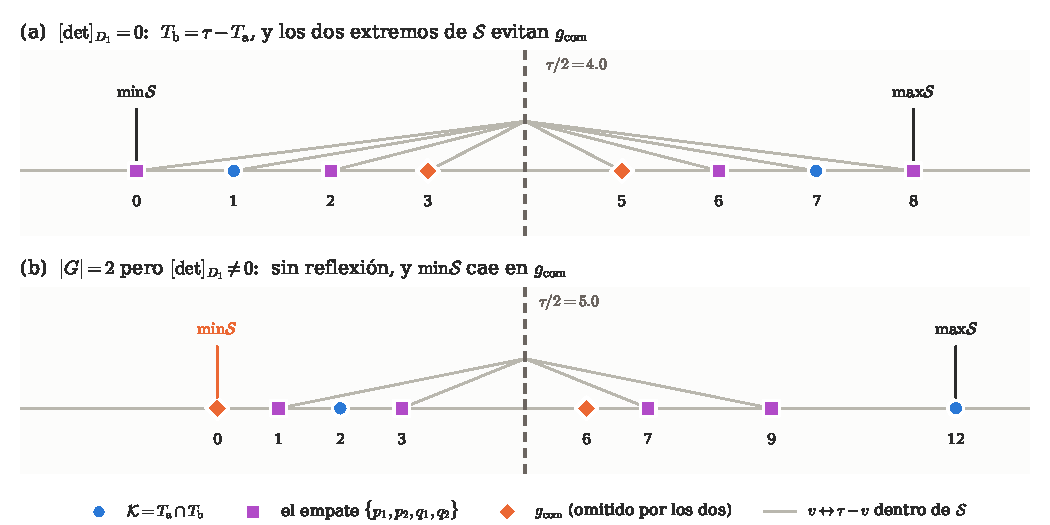
\includegraphics[width=\textwidth]{fig_reflection_es.pdf}
\caption{El Corolario \ref{cor:reflectgen} y la Proposición \ref{prop:A1gen} sobre dos formas, las
dos con $t=4$, $r=2$ y $|G|=2$. Cada panel dibuja $\mathcal{S}$ sobre una recta, coloreada según a
qué parte de \eqref{eq:gcomgen} pertenece el valor; un arco une $v$ con $\tau-v$ cuando los dos están
en $\mathcal{S}$, y la línea discontinua es el centro $\tau/2$. \emph{(a)} $\beta=(8,7,6,5,3,2,1,0)$:
$\tau=8$, $\mathcal{K}=\{1,7\}$, $g_{\mathrm{com}}=\{3,5\}$, empate $\{0,2,6,8\}$. Aquí
$T_{\mathrm b}=\tau-T_{\mathrm a}$, así que $\mathcal{S}\setminus g_{\mathrm{com}}$ es simétrico
respecto de $\tau/2$, y los dos extremos de $\mathcal{S}$ evitan $g_{\mathrm{com}}$, luego
$C=0+8=\tau$. Aquí $g_{\mathrm{com}}=\{3,5\}$ resulta ser simétrico también ---el arco que une sus
dos miembros se dibuja como cualquier otro---, que es lo que la Conjetura \ref{conj:gcom} afirma en
general y lo que la \S\ref{sec:rigidity} no demuestra: la reflexión queda establecida sobre
$\mathcal{S}\setminus g_{\mathrm{com}}$ y observada en el resto.
\emph{(b)} $\beta=(12,9,7,6,3,2,1,0)$: aquí $\tau=10$, y otra vez $|G|=2$, pero los dos maximizadores no
son reflexión uno de otro; $\min\mathcal{S}=0$ cae en $g_{\mathrm{com}}$, y $C=0+12=12\neq\tau$. El
panel (b) es la razón de que la Proposición \ref{prop:A1gen} no pueda demostrarse sólo a partir de
$|G|=2$. Calculada por \texttt{anc/fig\_v2.py}.}
\label{fig:reflection}
\end{figure}


\begin{proposition}[los extremos evitan la parte común]\label{prop:A1gen}
Supóngase $\bigl[\det(x_i^{\beta_j})\bigr]_{D_1}=0$. Entonces
$\max\mathcal{S}\notin g_{\mathrm{com}}$ y $\min\mathcal{S}\notin g_{\mathrm{com}}$.
\end{proposition}

\begin{proof}
Por el Corolario \ref{cor:reflectgen}, $T_{\mathrm b}=\tau-T_{\mathrm a}$. Como $x\mapsto\tau-x$
invierte el orden, lleva la mitad de abajo de $T_{\mathrm a}$ a la de arriba de $T_{\mathrm b}$ y al
revés:
\begin{equation}\label{eq:halvesgen}
  H_{\mathrm b}=\tau-L_{\mathrm a},\qquad L_{\mathrm b}=\tau-H_{\mathrm a}.
\end{equation}
Recuérdese del Paso 2 de la prueba del Teorema \ref{thm:Ggen} que un maximizador queda descrito por
los enteros $k_i$: dentro de la clase $i$, leída en orden decreciente, los primeros $k_i$ valores de
exceso están en la mitad de arriba, el siguiente es el omitido $g_i$, y los restantes están en la
mitad de abajo. Recuérdese también del Teorema \ref{thm:Ggen}(a) que un maximizador selecciona todo
incremento $>\tau$, que los incrementos de una clase se seleccionan en orden de prefijo, y que los
únicos incrementos iguales a $\tau$ son los dos empatados, que viven en las dos clases empatadas.

\emph{El máximo.} Póngase $m=\max\mathcal{S}$ y sea $i$ su clase, de modo que $m=c_{i,1}$ y
$n_i\ge2$; escríbase $c=c_{i,2}$. Entonces $m\in g_{\mathrm a}\cap g_{\mathrm b}$ si y sólo si
$k_i=0$ en los dos maximizadores. Supóngase que sí. Entonces la clase $i$ no está empatada: un
maximizador que toma el incremento empatado de una clase empatada tiene allí $k_i\ge1$. Luego ningún
incremento de la clase $i$ es $\ge\tau$ y, en particular,
\[
  \Delta_i(1)=m+c<\tau .
\]
Por otro lado $k_i=0$ coloca $c$ en la mitad de abajo de los dos maximizadores, así que
$c\in L_{\mathrm b}$, y \eqref{eq:halvesgen} da $\tau-c\in H_{\mathrm a}\subseteq\mathcal{S}$, de
donde $\tau-c\le\max\mathcal{S}=m$, esto es $\tau\le m+c$. Las dos desigualdades mostradas se
contradicen.

\emph{El mínimo} es la imagen especular. Póngase $m^{-}=\min\mathcal{S}$, sea $i^{-}$ su clase,
$n=n_{i^{-}}\ge2$ y $c'=c_{i^{-},n-1}$, de modo que $m^{-}=c_{i^{-},n}$. Entonces
$m^{-}\in g_{\mathrm a}\cap g_{\mathrm b}$ si y sólo si $k_{i^{-}}=n-1$ en los dos, es decir si y
sólo si los dos maximizadores seleccionan \emph{todos} los incrementos de la clase $i^{-}$; otra vez
la clase $i^{-}$ no puede estar empatada, ya que el maximizador que no toma el incremento empatado de
una clase empatada omite allí uno. Luego todo incremento de la clase $i^{-}$ supera a $\tau$, en
particular $\Delta_{i^{-}}(n-1)=m^{-}+c'>\tau$. Y $k_{i^{-}}=n-1$ coloca $c'$ en la mitad de arriba
de los dos, así que $c'\in H_{\mathrm b}$, y \eqref{eq:halvesgen} da
$\tau-c'\in L_{\mathrm a}\subseteq\mathcal{S}$, de donde $\tau-c'\ge\min\mathcal{S}=m^{-}$, esto es
$\tau\ge m^{-}+c'$. Contradicción.
\end{proof}

\begin{corollary}[el centro es el valor del empate]\label{cor:Ctaugen}
Si $\bigl[\det(x_i^{\beta_j})\bigr]_{D_1}=0$ entonces $C:=\min\mathcal{S}+\max\mathcal{S}=\tau$, y
$\mathcal{S}$ corta a todas las clases de residuos de las dos empatadas. Además $t$ es par y las dos
clases empatadas son exactamente las dos soluciones de $2\kappa\equiv C\pmod t$, ambas en
$\mathcal{E}$.
\end{corollary}

\begin{proof}
Por \eqref{eq:Ssymgen} el conjunto $\mathcal{S}\setminus g_{\mathrm{com}}$ es estable bajo
$x\mapsto\tau-x$, así que su mayor y su menor elemento suman $\tau$; por la Proposición
\ref{prop:A1gen} los dos extremos de $\mathcal{S}$ están en ese conjunto, luego \emph{son} su mayor y
su menor elemento, y $C=\tau$. El Teorema \ref{thm:Ggen}(b) da $t$ par y las dos clases empatadas
$i,i+t/2$, ambas en $\mathcal{E}$; por \eqref{eq:congrgen} $\tau\equiv2i\pmod t$, así que
$2\kappa\equiv\tau=C$ tiene exactamente las dos soluciones $\kappa=i$ y $\kappa=i+t/2$.
\end{proof}

\begin{corollary}[una condición necesaria, para todo $t$ par y todo $r$]\label{cor:necgen}
Sean $t\ge2$ y $r\ge1$, y supongamos $\Phi_{t,r}(\lambda;z)\equiv0$ con todo $n_i\ge1$. Entonces $t$
es par, $|G|=2$, $\min\mathcal{S}+\max\mathcal{S}=\tau$, y $\mathcal{S}\setminus g_{\mathrm{com}}$ es
simétrico respecto de $\tau/2$.
\end{corollary}

\begin{proof}
$\Phi_{t,r}$ y el numerador difieren en un factor no nulo, así que el numerador se anula
idénticamente y en particular $\bigl[\det(x_i^{\beta_j})\bigr]_{D_1}=0$. Se aplican los Corolarios
\ref{cor:reflectgen} y \ref{cor:Ctaugen} y \eqref{eq:Ssymgen}.
\end{proof}

\noindent Esto es lo que sobrevive de las \S\S\ref{sec:extremal}--\ref{sec:rigidity} fuera de $t=2$.
Lo que \emph{no} da es el paso que cierra $t=2$: allí $e=2$ obliga a $g_{\mathrm{com}}=\varnothing$, y
la simetría de $\mathcal{S}\setminus g_{\mathrm{com}}$ pasa a ser la simetría del propio $\beta$. Para
$t\ge4$ la parte común $g_{\mathrm{com}}$ puede no ser vacía, y el argumento de arriba no dice nada
de ella: la reflexión queda establecida sólo sobre $\mathcal{S}\setminus g_{\mathrm{com}}$, de modo
que restringe a $\beta$ sin llegar a determinarlo. Que $g_{\mathrm{com}}$ sea simétrico también es lo
que muestran las medidas y lo que enuncia la Conjetura \ref{conj:gcom}; aquí no se demuestra.

\subsubsection*{La condición es suficiente, para todo \texorpdfstring{$t$}{t} y todo
\texorpdfstring{$r$}{r}}

Una condición necesaria invita a su recíproco, y la mitad se consigue de una pieza. La reflexión que
el Corolario \ref{cor:necgen} extrae del estrato superior resulta ser, cuando vale sobre todo
$\mathcal{S}$ y no sólo sobre una parte, una simetría de \emph{cada} término de la suma de Laplace y
no únicamente de los dos maximizadores; y una involución sin puntos fijos cancela lo que empareja.
Escribimos
\[
C:=\min\mathcal{S}+\max\mathcal{S},\qquad\text{y escribimos } x\mapsto C-x
\text{ para la reflexión que centra.}
\]

\begin{theorem}[la dirección suficiente, para todo $t$ y todo $r$]\label{thm:suff}
Sean $t\ge2$, $r\ge1$, $N=t+2r$, y supongamos ocupada toda clase de residuos. Supongamos que
\begin{equation}\label{eq:suffcond}
C-\mathcal{S}=\mathcal{S}
\qquad\text{y}\qquad
\Delta_i(k)=C\ \text{para algún } i\in\mathcal{E},\ k .
\end{equation}
Entonces $\Phi_{t,r}(\lambda;z)\equiv0$.
\end{theorem}

Las dos cláusulas hacen dos trabajos distintos, y conviene decir cuál es cuál antes de la prueba: la
primera hace que la reflexión \emph{actúe} sobre las transversales, y la segunda hace que esa acción
sea \emph{libre}. La Figura \ref{fig:pairing} es el mecanismo entero sobre una sola forma, con otra al
lado que cumple la primera cláusula y no la segunda.

\begin{figure}[!ht]
\centering
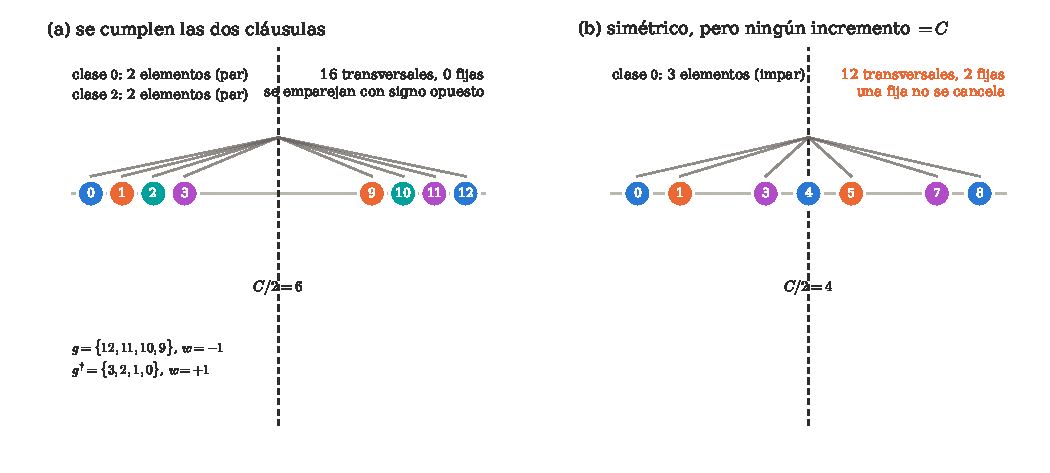
\includegraphics[width=\textwidth]{fig_pairing_es.pdf}
\caption{Por qué se cancela la suma, y para qué está la segunda cláusula. Cada panel dibuja
$\mathcal{S}$ sobre una recta, coloreado por clase de residuo, con un arco que une $v$ con $C-v$ y el
eje de puntos en $C/2$. \emph{(a)} $\beta=(12,11,10,9,3,2,1,0)$ con $t=4$, $r=2$: las dos clases que
la reflexión fija tienen tamaño \emph{par}, así que ninguna contiene a $C/2$; las $16$ transversales
se emparejan sin ningún punto fijo, y cada pareja lleva signos opuestos, de modo que cada término de
\eqref{eq:laplacegen} lo cancela otro. Una de esas parejas está impresa con sus dos signos,
calculados y no afirmados. \emph{(b)} una forma con $C-\mathcal{S}=\mathcal{S}$ pero sin ningún
incremento igual a $C$, encontrada buscándola y no elegida: allí la clase fija tiene tamaño
\emph{impar}, luego contiene a $C/2$, y dos transversales son su propio reflejo. Un término
emparejado consigo mismo no puede cancelarse, y la suma sobrevive. Eso es todo lo que compra la
segunda cláusula. Calculada por \texttt{anc/fig\_involution2.py}.}
\label{fig:pairing}
\end{figure}

\begin{lemma}[la transversal reflejada]\label{lem:reflact}
Supongamos $C-\mathcal{S}=\mathcal{S}$. Entonces $x\mapsto C-x$ lleva la clase $i$ sobre la clase
$i^{*}:=C-i \bmod t$, y o las dos están en $\mathcal{E}$ o ninguna; de modo que
\[
g^{\dagger}:=\bigl(C-(g\cap\mathcal{S})\bigr)\cup\bigl(g\setminus\mathcal{S}\bigr)
\]
es de nuevo una transversal, $g\mapsto g^{\dagger}$ es una involución sobre ellas, y
$T_{g^{\dagger}}=C-T_g$.
\end{lemma}

\begin{proof}
Todo elemento de la clase $i$ es $\equiv i$, así que $x\mapsto C-x$ lo manda dentro de la clase
$i^{*}$; como $C-\mathcal{S}=\mathcal{S}$ y la aplicación es inyectiva, lleva la clase $i$
\emph{sobre} la clase $i^{*}$ siempre que $i\in\mathcal{E}$, lo que obliga a $i^{*}\in\mathcal{E}$ y a
$n_i=n_{i^{*}}$. Las clases unitarias no se tocan: su único elemento está congelado en toda
transversal. Por último $T_{g^{\dagger}}=\mathcal{S}\setminus g^{\dagger}=C-(\mathcal{S}\setminus
g)=C-T_g$.
\end{proof}

\begin{lemma}[el menor reflejado]\label{lem:Arefl}
$A(C-T)=A(T)$ para todo $2r$-conjunto $T$ y todo $C$.
\end{lemma}

\begin{proof}
% Sin "=" en esta frase: TeX parte la formula en linea despues de la relacion y deja el signo
% colgando fuera del margen, y forzarla con \mbox la echa entera fuera.  Se dice con palabras.
Sacar $x_i^{C}$ de cada una de las $2r$ filas multiplica el determinante por el factor
$\prod_j z_j^{C}z_j^{-C}$, que vale $1$, y deja la matriz de $T$ con $x_i$ sustituido por
$x_i^{-1}$, que es la
matriz de $T$ con las dos filas de cada par recíproco intercambiadas: un signo $(-1)^{r}$.
Y listar $C-T$ en orden decreciente invierte el orden de las columnas, lo que aporta
$(-1)^{\binom{2r}{2}}$, es decir $(-1)^{r}$, porque $2r-1$ es impar. Los dos se cancelan.
\end{proof}

\noindent Los dos movimientos de esa prueba no son nuestros, y merece la pena decir de quién son,
porque son el instrumento adecuado y los elegimos por eso. Escalar cada fila por una potencia para
sustituir $x_i$ por $\bar x_i$, y luego invertir un bloque de columnas para recoger
$(-1)^{n(n-1)/2}$, es la maniobra que Ayyer y Behrend emplean sobre el bialternante de una forma
autocomplementaria \cite[\S3]{AB19}; ellos mismos describen sus pruebas como apoyadas sólo en las
expresiones determinantales ``y la aplicación de operaciones estándar con determinantes'', y ésta es
una de esas operaciones. Albion hace la misma inversión del lado de las raíces de la unidad
\cite{Alb23,Alb25}, y a nivel de caracteres el mismo hecho es la invariancia de $sp_\lambda$ bajo
$x_i\mapsto\bar x_i$, recogida en \cite{AB19} y puesta a trabajar en \cite{AF20}.

Conviene explicar por qué es útil aquí, porque es lo que hace corta toda la sección. A un menor
reflejado se le puede atacar desarrollándolo, y entonces habría que seguir término a término las
clases unitarias y las reflejadas --- que es como lo intentamos primero, y no se acaba nunca. La
maniobra de Ayyer y Behrend, en cambio, liquida la reflexión en \emph{dos} cálculos de signo que no
miran las entradas en ningún momento, y es robusta justo en el sentido que necesitamos: no usa en
ningún paso que se esté reflejando el alfabeto entero, así que sobrevive al aplicarse a una
\emph{parte} del conjunto beta, con el resto quieto. Esa robustez es la razón de que el Lema
\ref{lem:Arefl} ocupe cuatro líneas y no una sección, y pertenece a la herramienta y no a nosotros.
Es además un indicio menor a favor de la tesis de la \S\ref{sec:background}: las dos líneas entre las
que se sitúa este artículo comparten más maquinaria de lo que sus enunciados dejan ver.

El enunciado que sigue es el corazón combinatorio del argumento, y sólo necesita la primera cláusula
de \eqref{eq:suffcond}. Reflejar un conjunto beta \emph{entero} es clásico --- es la identidad de
complementación \eqref{eq:compl}, y los pasos determinantales que hay detrás son los estándar que
acabamos de citar. Lo que aquí se pide es la reflexión de la parte de exceso \emph{sola}, con las
clases unitarias quietas e intercaladas entre los valores reflejados; las dos involuciones que eso
produce, una de $\beta$ y otra de $\ZZ/t$, son de las que acaba dependiendo el signo.

\begin{lemma}[la fórmula del signo de la reflexión parcial]\label{lem:signformula}
Supongamos $C-\mathcal{S}=\mathcal{S}$, y pongamos
\[
\nu=\#\{x\in\mathcal{S}:2x=C\},\qquad \eta=\#\{i\in\mathcal{E}:2i\equiv C \bmod t\}.
\]
Entonces, para toda transversal $g$,
\begin{equation}\label{eq:wrefl}
\frac{w(g^{\dagger})}{w(g)}\;=\;(-1)^{\,e-\frac{\nu+\eta}{2}} .
\end{equation}
En particular el cociente no depende de $g$, ni de $r$, ni de $N$.
\end{lemma}

\begin{corollary}\label{cor:whenminus}
Bajo $C-\mathcal{S}=\mathcal{S}$, el cociente \eqref{eq:wrefl} vale $-1$ si y sólo si $\eta=2$.
\end{corollary}

\begin{proof}
Una involución tiene tantos puntos fijos como elementos su conjunto, módulo dos, así que
$\nu\equiv|\mathcal{S}|$ y $\eta\equiv e$; y $|\mathcal{S}|=2r+e$ por \eqref{eq:excessgen}, luego
también $\nu\equiv e$. Si $e$ es impar, entonces $\nu=\eta=1$ y el exponente es $e-1$, par. Si $e$ es
par, entonces $\nu=0$ y $\eta$ vale $0$ ó $2$, lo que da el exponente $e$ ó $e-1$; el primero es par y
el segundo impar.
\end{proof}

\noindent Esa independencia es la parte que parece improbable y es justo la que importa: las clases
unitarias están colocadas en posiciones arbitrarias entre los valores reflejados, y mover una
transversal las hace cruzarse unas con otras --- pero cada cruce que aportan a la suma de columnas lo
deshace el cruce que aportan a la palabra de residuos, así que no dejan rastro en el cociente.

\begin{lemma}[el signo reflejado]\label{lem:signrefl}
Supongamos \eqref{eq:suffcond}. Entonces $\eta=2$, el número $e$ es par, $\nu=0$, y
$w(g^{\dagger})=-w(g)$ para toda transversal $g$.
\end{lemma}

\begin{proof}[Prueba del Lema \ref{lem:signformula}]
Sea $\mathcal{R}$ la aplicación $x\mapsto C-x$ sobre $\mathcal{S}$ y la identidad sobre
$\beta\setminus\mathcal{S}$, y sea $\mathcal{R}_t$ la aplicación $i\mapsto i^{*}$ sobre $\mathcal{E}$
y la identidad fuera; ambas son involuciones, de $\beta$ y de $\ZZ/t$ respectivamente, con $\nu$ y
$\eta$ puntos fijos, así que $\sgn(\mathcal{R})=(-1)^{(|\mathcal{S}|-\nu)/2}$ y
$\sgn(\mathcal{R}_t)=(-1)^{(e-\eta)/2}$. Ordenemos las columnas de una transversal $g$ por residuo y
las restantes por $\beta$ decreciente; el signo de la permutación de $\{1,\dots,N\}$ que resulta es
$w(g)$ salvo un factor que depende sólo de $t$. Aplicar $\mathcal{R}$ a esa notación de una línea
aporta $\sgn(\mathcal{R})$; restablecer el orden por residuo del primer bloque aporta
$\sgn(\mathcal{R}_t)$; y $\mathcal{R}$ invierte $T_g$ por completo, de modo que restablecer su orden
decreciente aporta $(-1)^{\binom{2r}{2}}$. Multiplicando los tres sale \eqref{eq:wrefl}, donde ningún
término se refiere a $g$.
\end{proof}

\begin{proof}[Prueba del Lema \ref{lem:signrefl}]
Contar puntos fijos de una involución da $|\mathcal{S}|\equiv\nu$ y $e\equiv\eta \pmod 2$, y
$|\mathcal{S}|=2r+e$ por \eqref{eq:excessgen}, luego $e\equiv\nu$. Ahora bien, la segunda cláusula de
\eqref{eq:suffcond} dice que dos elementos \emph{adyacentes} de alguna clase $i_0$ suman $C$; la
reflexión los intercambia, así que $i_0=i_0^{*}$, y escribiendo la clase en orden decreciente el
intercambio manda su $k$-ésima entrada a la $(n_{i_0}+1-k)$-ésima, de donde $n_{i_0}=2k$ es par. La
reflexión $x\mapsto C-x$ tiene a lo sumo un punto fijo, que es $C/2$; como esta clase es estable bajo
ella y tiene cardinal par, sus elementos se emparejan y no contiene ninguno, luego $C/2\notin$ clase
$i_0$.

Antes de hablar de una segunda solución hay que saber que la hay, y ahí es donde la paridad de $t$ se
decide en vez de suponerse. Supongamos $t$ impar. Entonces $2$ es invertible módulo $t$, así que
$i\mapsto i^{*}$ tiene a $i_0$ como su \emph{único} residuo fijo; las demás clases de $\mathcal{E}$ se
emparejan, luego $e$ es impar, y $|\mathcal{S}|=2r+e$ también. Una involución sobre un conjunto de
tamaño impar tiene un punto fijo, así que $\nu=1$ y $C/2\in\mathcal{S}$; su residuo $\kappa$ cumple
$2\kappa\equiv C$, luego $\kappa=i_0$, lo que sitúa a $C/2$ en la clase $i_0$ --- que acabamos de ver
que no lo contiene. Así que $t$ es par, y $2i\equiv C$ tiene exactamente las dos soluciones $i_0$ e
$i_1=i_0+t/2$.

Si $\nu=1$, entonces $C/2\in\mathcal{S}$ y su residuo es $i_0$ o $i_1$; no es $i_0$, luego
$i_1\in\mathcal{E}$. Si $\nu=0$, entonces $e$ es par, y $\mathcal{E}=\{i_0\}\sqcup\{\text{pares}\}$
haría $e$ impar salvo que $i_1\in\mathcal{E}$. En cualquiera de los dos casos $\eta=2$, luego $e$ es
par y $\nu=0$, y el Corolario \ref{cor:whenminus} da el signo de inmediato. Leyendo \eqref{eq:wrefl}
directamente, el exponente es $e-\tfrac{0+2}2=e-1\equiv1 \pmod 2$.
\end{proof}

\begin{corollary}[la hipótesis, leída sobre los residuos]\label{cor:suffgeom}
Supongamos $C-\mathcal{S}=\mathcal{S}$. Entonces algún $\Delta_i(k)=C$ si y sólo si $t$ es par y
\emph{las dos} soluciones de $2i\equiv C \pmod t$ son clases de exceso. Dicho de otro modo,
\eqref{eq:suffcond} afirma: la parte de exceso del conjunto beta es simétrica respecto de $C/2$, y las
dos clases de residuos que la reflexión fija son ambas de exceso.
\end{corollary}

\begin{proof}
Una dirección es el primer párrafo de la prueba del Lema \ref{lem:signrefl}. Para la otra, si las dos
clases fijas están en $\mathcal{E}$ entonces $\eta=2$, luego $e$ es par por $e\equiv\eta$, luego
$|\mathcal{S}|=2r+e$ es par y $\nu=0$: ningún elemento de $\mathcal{S}$ queda fijo. Una clase fija es
entonces estable por la reflexión y sin puntos fijos, luego de tamaño par $2k$, y sus entradas
$k$-ésima y $(k+1)$-ésima se intercambian, así que $\Delta_i(k)=C$.
\end{proof}

\noindent Leída así, la hipótesis tiene la misma forma que la conclusión del Corolario
\ref{cor:Ctaugen}, y eso es lo que hace que las dos mitades de la sección se miren la una a la otra:
allí las dos clases empatadas \emph{resultan} ser las dos soluciones de $2\kappa\equiv C$; aquí
\emph{pedimos} que sean de exceso.

\begin{proof}[Prueba del Teorema \ref{thm:suff}]
Por el Lema \ref{lem:reflact}, $g\mapsto g^{\dagger}$ es una involución sobre las transversales con
$T_{g^{\dagger}}=C-T_g$. No tiene puntos fijos: una transversal fija necesitaría $C-g_i=g_i$, es
decir $g_i=C/2$, en toda clase con $i=i^{*}$, y la clase $i_0$ de la prueba anterior es una de ésas y
no contiene a $C/2$. Por los Lemas \ref{lem:Arefl} y \ref{lem:signrefl},
\[
w(g)A(T_g)+w(g^{\dagger})A(T_{g^{\dagger}})=w(g)A(T_g)-w(g)A(C-T_g)=0 ,
\]
así que la suma de \eqref{eq:laplacegen} se cancela por parejas y el numerador se anula
idénticamente.
\end{proof}

\begin{remark}[qué es esto, y qué no es]\label{rem:suffscope}
Conviene separar tres cosas. Primera: en $t=2$ la hipótesis \eqref{eq:suffcond} \emph{es} la rama
{\rm(b)}; allí $e=2$ obliga a $\mathcal{S}=\beta$, con lo que $C-\mathcal{S}=\mathcal{S}$ es la
autocomplementariedad, y la cláusula del incremento es la paridad de la anchura --- los dos enunciados
coinciden en todas las formas de los rangos de la \S\ref{sec:verif}. Así que el Teorema
\ref{thm:suff} contiene esa mitad del Teorema \ref{conj:crit}, y la prueba otra vez por un mecanismo
distinto. Segunda: para $t\ge4$ \emph{no} es complementación; allí $\mathcal{S}\subsetneq\beta$,
$\lambda$ no es autocomplementaria, y \eqref{eq:compl} no dice nada. Tercera: la involución es global
--- empareja \emph{todos} los términos de \eqref{eq:laplacegen} y no sólo los dos maximizadores ---, y
por eso sobrevive donde el argumento extremal sólo produce una condición necesaria.
\end{remark}

\begin{conjecture}[el criterio, en general]\label{conj:general}
Recíprocamente, si $\Phi_{t,r}(\lambda;z)\equiv0$ y toda clase de residuos está ocupada, entonces vale
\eqref{eq:suffcond}. Equivalentemente, para todo $t$ y todo $r$,
\[
\Phi_{t,r}(\lambda;z)\equiv0
\iff
\text{alguna clase es vacía, o } C-\mathcal{S}=\mathcal{S}\text{ y algún }\Delta_i(k)=C .
\]
\end{conjecture}

\noindent Bajo la hipótesis de anulación, casi todo lo que pide \eqref{eq:suffcond} ya se sabe, y
decir qué parte convierte la conjetura en una sola frase sobre un solo conjunto. El Corolario
\ref{cor:Ctaugen} da $C=\tau$, luego los incrementos empatados valen $C$ y la segunda cláusula se
cumple; y \eqref{eq:Ssymgen} da $C-(\mathcal{S}\setminus g_{\mathrm{com}})=\mathcal{S}\setminus
g_{\mathrm{com}}$. Como $\mathcal{S}=(\mathcal{S}\setminus g_{\mathrm{com}})\sqcup g_{\mathrm{com}}$,
lo único que queda es esto:

\begin{conjecture}[la parte común es simétrica]\label{conj:gcom}
Bajo ocupación, si $\Phi_{t,r}(\lambda;z)\equiv0$ entonces $C-g_{\mathrm{com}}=g_{\mathrm{com}}$.
\end{conjecture}

\noindent Las Conjeturas \ref{conj:general} y \ref{conj:gcom} son el mismo enunciado, y la segunda es
la forma útil: nombra los $e-2$ elementos a los que el argumento tiene que llegar, y ningunos más.
Dice también, de una vez, por qué $t=2$ cierra y $t\ge4$ no. En $t=2$ un empate es entre las clases
$i$ e $i+1$, de modo que las dos son de exceso y $e=2$ ---no porque allí $e=2$ valga siempre, pues
\eqref{eq:excessgen} permite $e=1$ y es frecuente, sino porque $|G|=2$ lo obliga, y
$g_{\mathrm{com}}$ sólo está definido cuando $|G|=2$---. Por tanto $g_{\mathrm{com}}=\varnothing$ y
no queda nada que pueda ser simétrico. El teorema no es allí más
fácil; sencillamente no hay parte común.

Los enunciamos como conjeturas y no como teoremas porque sólo está probada la dirección de arriba. La
evidencia está en la \S\ref{sec:verif}: sobre $190\,443$ formas en veinticuatro configuraciones, con
$t\le12$ y $r\le4$, el criterio no tiene ningún falso positivo ni ningún falso negativo; $43\,010$
de ellas se rehacen con una evaluación que no comparte código con esta sección, y un barrido más de
$12\,937$ formas, con $131$ ceros, se rehace en Sage, que no comparte con ninguna de las dos ni
código ni biblioteca; en los rangos donde ya
decide un teorema, coincide con el Teorema \ref{thm:main} en $r=1$ y con el Teorema \ref{conj:crit} en
$t=2$ sin una sola discrepancia, sobre $9913$ y $29\,508$ formas; y un señuelo que lee la condición
sobre $\beta$ en vez de sobre $\mathcal{S}$ --- esto es, la autocomplementariedad de la forma en lugar
de la de su parte de exceso --- falla en todas las configuraciones de ambos barridos. Lo que falta es
una implicación: el Corolario \ref{cor:necgen} da la reflexión sobre $\mathcal{S}\setminus
g_{\mathrm{com}}$, y el estrato superior no puede dar más --- hay formas que comparten $\tau$,
$\mathcal{S}\setminus g_{\mathrm{com}}$ y las clases empatadas, y de las cuales unas se anulan y otras
no, así que la ecuación que falta no es un refinamiento de la \S\ref{sec:rigidity} sino un enunciado
sobre un estrato inferior.

\begin{remark}[por qué no el argumento obvio]
Lo primero que se intenta es un intercambio dentro de un \emph{solo} maximizador: si
$\max\mathcal{S}$ está omitido, re-elegir su clase y esperar que suba el grado. No puede funcionar.
Un maximizador puede omitir $\max\mathcal{S}$ --- justo cuando $\max\mathcal{S}$ es uno de los valores
empatados $p_1,p_2$, de modo que un maximizador lo omite y el otro lo conserva ---, así que ningún
argumento que lea una transversal cada vez concluye. La Proposición \ref{prop:A1gen} es un enunciado
sobre el \emph{par}, y por eso la prueba corre sobre \eqref{eq:halvesgen} y sobre nada más. El Cuadro
\ref{tab:extremal} recoge tanto los pasos de esa prueba como lo que le pasa a su conclusión cuando se
quita la hipótesis.
\end{remark}

\begin{table}[!ht]
\centering\small
\caption{La maquinaria de las \S\S\ref{sec:extremal}--\ref{sec:rigidity}, medida. La población es
toda forma con $|G|=2$ sobre $(t,r)\in\{4,6,8,10\}\times\{2,3\}$ dentro de las anchuras barridas. La
última fila es la que importa para la Proposición \ref{prop:A1gen}: al quitar la hipótesis
$[\det]_{D_1}=0$ la conclusión falla, así que no viene de balde.}
\label{tab:extremal}
\begin{tabular}{@{}llrl@{}}
\toprule
enunciado & población & resultado & guion \\
\midrule
\rowcolor{hband} parametrización voraz $=$ fuerza bruta & $4049$ formas & \textcolor{hproved}{$0$ fallos} & \texttt{a1\_proof} \\
$A$ es la mitad de arriba de $T_g$ (Paso 2) & la misma & \textcolor{hproved}{$0$ fallos} & \texttt{a1\_proof} \\
\rowcolor{hband} $T_{\mathrm b}=\tau-T_{\mathrm a}$ & $2522$ formas & \textcolor{hproved}{$0$ fallos} & \texttt{a1\_proof} \\
$v\in L_{\mathrm b}\Rightarrow\tau-v\in H_{\mathrm a}$ & $3034$ valores & \textcolor{hproved}{$0$ fallos} & \texttt{a1\_proof} \\
\rowcolor{hband} los extremos evitan $g_{\mathrm{com}}$ & $2522$ formas & \textcolor{hproved}{$0$ fallos} & \texttt{a1\_proof} \\
las identidades mostradas de estas subsecciones & $11$ identidades & \textcolor{hproved}{$0$ fallos} & \texttt{v2\_formulas} \\
\midrule
\rowcolor{hband} lo mismo, quitando $[\det]_{D_1}=0$ & $24718$ formas & \textcolor{hverif}{$414$ fallos} & \texttt{a1\_proof} \\
\bottomrule
\end{tabular}
\end{table}

\begin{remark}
El Corolario \ref{cor:reflectgen} hace trabajo de verdad en la Proposición \ref{prop:A1gen}, y
$|G|=2$ por sí solo no basta. Para $t=4$, $r=2$ y $\beta=(200,199,198,197,194,193,191,4)$ las clases
de exceso son $\{200,4\}$, $\{197,193\}$, $\{198,194\}$, $\{199,191\}$ y los incrementos son
$392,390,390,204$, así que $\tau=390$, el empate es entre las clases $1$ y $3$, y $|G|=2$. Pero
$\Delta_0(1)=204<\tau$, así que $k_0=0$ en los dos maximizadores y $\max\mathcal{S}=200$ lo omiten los
dos: la conclusión de la Proposición \ref{prop:A1gen} falla. Aquí $T_{\mathrm a}=(198,197,191,4)$ y
$T_{\mathrm b}=(199,198,193,4)$ no son reflexión una de otra --- $h_r-l_1$ vale $6$ para la primera y
$5$ para la segunda --- y en consecuencia la componente de grado $D_1$ no se anula.
\end{remark}

\begin{figure}[!ht]
\centering
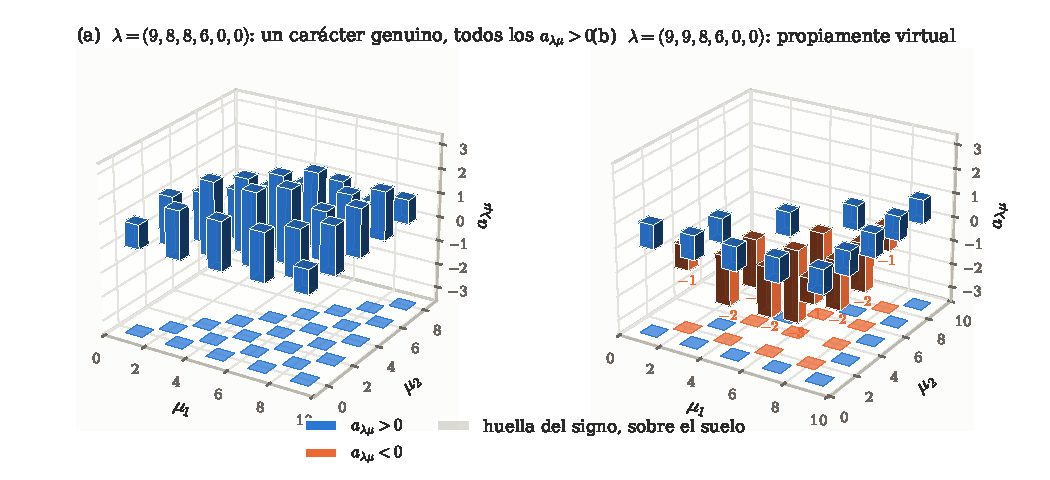
\includegraphics[width=\textwidth]{fig_virtual_es.pdf}
\caption{Por qué un solo par recíproco no es lo típico, en $r=2$: la expansión
$\Psi_r(\lambda)=\sum_\mu a_{\lambda\mu}\,sp_\mu(z)$ sobre los pesos dominantes de $Sp(4)$. Las dos
formas difieren en una sola casilla. Para $\lambda=(9,8,8,6,0,0)$ todo $a_{\lambda\mu}$ es positivo:
el objeto es un carácter genuino, como lo es para \emph{toda} $\lambda$ cuando $r=1$, donde el
Teorema \ref{thm:main} lo escribe como producto de tres caracteres de $\mathfrak{sl}_2$. Para
$\lambda=(9,9,8,6,0,0)$ la expansión tiene $12$ coeficientes positivos y $10$ negativos, siendo el más
negativo $-3$: es genuinamente virtual, que es el fenómeno que recoge la Observación
\ref{rem:rankone} y la razón de que un cálculo en el extremo deje de ser un test exacto pasado un
par. Los dos paneles comparten la escala vertical, y los cuadrados planos del suelo repiten el signo
de cada coeficiente, porque un coeficiente $-1$ es invisible al lado de uno $+3$. Calculada por
\texttt{anc/fig\_v2.py}.}
\label{fig:virtual}
\end{figure}

\subsubsection*{El criterio en \texorpdfstring{$t=2$}{t=2}}

\begin{proof}[Demostración del Teorema \ref{conj:crit}]
La implicación de (a) o (b) a $\Psi_r(\lambda)=0$ es el Teorema \ref{thm:zeros}. Para el recíproco,
supóngase $\Psi_r(\lambda)=\Phi_{2,r}(\lambda;z)\equiv0$ y que ninguna clase de residuos módulo $2$
falta en $\beta(\lambda)$, ya que en otro caso se cumple la rama (a) y no hay nada que probar.
Entonces el numerador se anula idénticamente, así que en particular su componente de grado $D_1$ se
anula y $|G|=2$ por el Corolario \ref{cor:uniquegen}.

Por el Teorema \ref{thm:Ggen}(b) hay un empate en el rango $r$ entre las clases $i$ e $i+t/2=i+1$; en
$t=2$ ésas son las dos clases, y ambas están en $\mathcal{E}$, luego $e=2$. (Con $e=1$ todos los
incrementos viven en una sola clase y son distintos dos a dos por el Paso 4, así que no hay empate
posible.) Como $e=2$, ninguna clase es unitaria y $\mathcal{S}=\{\beta_1,\dots,\beta_N\}$ es el
beta-conjunto entero.

Por el Corolario \ref{cor:Ctaugen}, $C=\min\mathcal{S}+\max\mathcal{S}=\beta_N+\beta_1=\tau$ y, como
cambian las dos clases, $g_{\mathrm{com}}=\varnothing$ en \eqref{eq:gcomgen}, de modo que
\eqref{eq:Ssymgen} se lee $\tau-\mathcal{S}=\mathcal{S}$: el beta-conjunto es simétrico respecto de
$C$, es decir
\[
  \beta_j+\beta_{N+1-j}=C\qquad\text{para todo }j .
\]
Sustituyendo $\beta_j=\lambda_j+N-j$ esto se convierte en $\lambda_j+\lambda_{N+1-j}=C-N+1=:w$ para
todo $j$, que es la auto-complementariedad de anchura $w=\lambda_1+\lambda_N$. Finalmente, el
Corolario \ref{cor:Ctaugen} dice que las dos soluciones de $2\kappa\equiv C\pmod2$ son las dos
clases, lo que ocurre exactamente cuando $C$ es par; y $C=w+N-1$ con $N=2r+2$ par, así que $C$ par es
exactamente $w$ impar. Luego $\lambda$ es auto-complementaria de anchura impar: la rama (b).
\end{proof}

\begin{remark}
En $t=2$ la congruencia \eqref{eq:congrgen} es vacua --- todo incremento es par --- y $|G|\le2$ vale
por la razón más débil de que sólo existen dos clases. Lo que \emph{no} es vacuo en $t=2$ es que
$\tau$ sea par, y se usa dos veces: prohíbe el emparejamiento cruzado en la Proposición
\ref{prop:centregen}, y \emph{es} la paridad que se convierte en la rama (b).
\end{remark}

\begin{remark}[\emph{genuino} no quiere decir \emph{irreducible}]
En la Observación \ref{rem:rankone}, \emph{$\pm$ un carácter genuino} significa una combinación
\emph{no negativa} de irreducibles, no uno solo. No es uno solo: ya
$s_{(2)}(1,-1,z,z^{-1})=z^{2}+2+z^{-2}=sp_{(2)}+sp_{(0)}$. En $t=2$, $r=1$ el Teorema
\ref{thm:main} da un producto de tres caracteres de $\mathfrak{sl}_2$, y un producto de caracteres es
un carácter --- ésa es toda la afirmación. A partir de $r=2$ aparecen coeficientes negativos y no
existe ninguna representación, que es lo que quiere decir \emph{genuinamente virtual}; el Cuadro
\ref{tab:virtual} cuenta las dos cosas y la Figura \ref{fig:virtual} dibuja una de cada.
\end{remark}

\begin{table}[!ht]
\centering\small
\caption{Genuino frente a genuinamente virtual, sobre todas las $\lambda$ con $\lambda_1$ hasta la
cota indicada. La expansión es $\Psi_r(\lambda)=\sum_\mu a_{\lambda\mu}\,sp_\mu(z)$; \emph{un signo}
quiere decir que todos los $a_{\lambda\mu}$ tienen el mismo signo, de modo que $\pm\Psi_r$ es un
carácter, y \emph{mezclado} quiere decir que es genuinamente virtual. En $r=1$ la columna de mezclados
está vacía, como fuerza el Teorema \ref{thm:main}; no lo está para ningún $r\ge2$ al que lleguemos.
Calculada por \texttt{anc/fig\_v2.py}.}
\label{tab:virtual}
\begin{tabular}{@{}lrrrr@{}}
\toprule
 & \multicolumn{1}{c}{formas} & \multicolumn{1}{c}{$\Psi_r=0$} & \multicolumn{1}{c}{un signo}
 & \multicolumn{1}{c}{mezclado} \\
\midrule
\rowcolor{hband} $r=1$, $\lambda_1\le14$ & $3060$ & $352$ & $2708$ & \textcolor{hproved}{$\mathbf{0}$} \\
$r=2$, $\lambda_1\le8$  & $3003$ & $78$ & $2531$ & \textcolor{hverif}{$\mathbf{394}$} \\
$r=3$, $\lambda_1\le5$  & $1287$ & $27$ & $1008$ & \textcolor{hverif}{$\mathbf{252}$} \\
$r=4$, $\lambda_1\le2$  & $66$   & $2$  & $58$   & \textcolor{hverif}{$\mathbf{6}$} \\
\bottomrule
\end{tabular}
\end{table}

\begin{remark}[dónde vive el alfabeto]
Para $r=1$ el alfabeto $(1,-1,z,\bar z)$ de \eqref{eq:psir} es literalmente la lista de valores
propios de una matriz de la componente no identidad $O(4)^{-}$, tabulada como tal por Hanany y
Kalveks \cite[Tabla 7]{HK16}, que además registran la caída de rango
$[\mathrm{vec}]_{O(2n)^{-}}\cong[\mathrm{vec}]_{O(2)^{-}}\oplus[\mathrm{fund}]_{C_{n-1}}$ para la
representación \emph{vectorial}. Así que $\Psi_r$ es un carácter de $GL(2r+2)$ evaluado en esa
componente, y el plegado $D_{r+1}\to C_r$ es la razón de que aparezca un grupo simpléctico; no lo
usamos más que para situar el objeto, ya que para una $\lambda$ cualquiera la restricción es una
combinación con coeficientes enteros de caracteres simplécticos, y no uno solo.
\end{remark}

\section{Verificación}\label{sec:verif}

Todos los enunciados anteriores se comprobaron numéricamente, con tres implementaciones por rutas de
código distintas: una en aritmética de Laurent exacta, otra una evaluación del bialternante escrita
desde cero a partir de los enunciados, y una tercera en Sage, que no comparte con las otras dos ni
una línea de código ni una biblioteca. Los rangos y recuentos se recogen aquí una sola vez.

% longtable y no tabular: con un tabular esta tabla es una caja indivisible, y LaTeX la empuja
% entera a la pagina siguiente dejando la de la cabecera de seccion casi vacia.  longtable parte por
% paginas y repite la cabecera, que es lo que una tabla de cuarenta filas necesita.
% \raggedright en las dos primeras: justificadas, una columna estrecha estira los espacios y deja
% "t <= 7, |lambda| <=" con huecos enormes.  La tercera va \raggedleft porque son cifras.
\begingroup\footnotesize\setlength{\tabcolsep}{4.0pt}
% Anchuras algo menores que en la edicion inglesa: el castellano es mas largo por palabra y con las
% de alla la tabla se salia 4 pt.  Se miden en el PDF, no en el log.
\begin{longtable}{@{}>{\raggedright\arraybackslash}p{0.352\linewidth}%
                  >{\raggedright\arraybackslash}p{0.222\linewidth}%
                  >{\raggedleft\arraybackslash}p{0.272\linewidth}@{\hspace{4pt}}l@{}}
\toprule
enunciado & rango & resultado & estado\\
\midrule
\endfirsthead
\multicolumn{4}{@{}l}{\footnotesize\itshape Verificación, continuación}\\[1pt]
\toprule
enunciado & rango & resultado & estado\\
\midrule
\endhead
\midrule
\multicolumn{4}{r@{}}{\footnotesize\itshape sigue en la página siguiente}\\
\endfoot
\bottomrule
\endlastfoot
Teor. \ref{thm:main}, signo incluido & $t\le7$, $|\lambda|\le14,\dots,10$ &
$959$ exactos, $476$ ceros, $0$ fallos & \stproved\\
\quad lo mismo, una implementación escrita desde el enunciado & $t\le6$, $|\lambda|\le12,\dots,9$ &
$749$ formas, $0$ fallos; el señuelo del signo falla $35/133$ & \stproved\\
Lema \ref{lem:L1} & $t\le6$ & $454$ menores no nulos & \stproved\\
Lema \ref{lem:L4} & $t\le7$ & $724/724$ & \stproved\\
Proposición \ref{prop:quotient} & $t\le7$, $|\lambda|\le19$ & $2970/2970$ & \stproved\\
Prop. \ref{rem:lattice} (lugar concéntrico) & $t\le9$, $|\lambda|\le16$ & $1331/1331$;
$0$ con $t$ impar, $43$ con par & \stproved\\
Prop. \ref{rem:sign} (forma corta del signo) & $t\le8$, $|\lambda|\le14$ & $1496/1496$;
pasos de la prueba, $0$ fallos & \stproved\\
\quad la ley de desplazamiento \eqref{eq:shift} y su signo & $t\le7$, $|\lambda|\le12$ &
$826$ formas, $0$ fallos & \stproved\\
Prop. \ref{prop:minimal} (el multiconjunto separa) & $d_i\le60$; $t\le5$, $|\lambda|\le16$ &
$75640$ invariantes, $0$ colisiones & \stproved\\
\quad lo mismo, en los dos sentidos, desde el enunciado & $t\le5$, $|\lambda|\le14,\dots,11$ &
$676$ formas, $0$ colisiones; señuelo $104$ & \stproved\\
Prop. \ref{prop:fibrelattice} (el retículo) & $t\le5$, $|\lambda|\le14,12,10,10$ &
$84$, $35$, $20$, $14$ fibras, en ambos sentidos & \stproved\\
Cor. \ref{cor:fibregf} (función generatriz) & mismo rango &
$153/153$; denominador erróneo $101$ & \stproved\\
Observación \ref{rem:signsees} (el signo ve los $m_i$) & $t\le4$ &
$107/107$, $43/62$, $26/36$ & \stverif\\
Lema \ref{lem:single} & $t\le7$, $|\lambda|\le16$ & $2113/2113$ & \stproved\\
Teor. \ref{thm:extra} & $t\le12$, $\lambda_1\le33$ & $119+21$, ninguna más & \stproved\\
\quad el signo es $+1$, \eqref{eq:extrainv} & $t\le14$ par; núcleos $t\le10$ &
$28$ extra $+$ $219$ núcleos, todos $+1$ & \stproved\\
Proposición \ref{prop:rect} & $t=2$, $r\le4$, $c\le60$ & $240/240$ & \stproved\\
Cor. \ref{cor:enum} contra enumeración directa & $t\le5$ & $14/14$; cajas $16/16$ &
\stproved\\
Prop. \ref{rem:involution} (las rachas alternan) & $t=2$, $|\lambda|\le14$, $\le4$ filas &
$4823$ menores; $217$ pares, $0$ fallos & \stproved\\
(D3), (D4) de la \S\ref{sec:sharp} & $t\le6$, $|\lambda|\le10$ &
$600$ / $383$ / $200$ de $600$ & \stverif\\
\midrule
\rowcolor{hband} Teor. \ref{conj:crit}, el criterio, todo $r$ & --- & prueba, \S\ref{sec:rigidity} & \stproved\\
\rowcolor{hband} \quad lo mismo, leído sobre $O(N)$, Cor.~\ref{cor:dettwist} & --- &
reformulación, \S\ref{sec:conv} & \stproved\\
\rowcolor{hband} \quad Teor. \ref{thm:PvW}, el input externo & --- & \cite{PvW} & \stext\\
\rowcolor{hband} \quad Teorema \ref{thm:Ggen}, $|G|\le2$ & $t\le10$, $r\le3$ & voraz contra fuerza bruta, $0/4049$ & \stproved\\
\rowcolor{hband} \quad Prop.~\ref{prop:A1gen}, los extremos & $t\le10$, $r\le3$ & $2522$ formas, $0$ fallos & \stproved\\
\rowcolor{hband} \quad \quad la hipótesis hace falta & mismo & $414$ formas fallan sin ella & \stproved\\
\rowcolor{hband} \quad las identidades mostradas, \S\S\ref{sec:extremal}--\ref{sec:rigidity} & $t=2$, $r\le3$ & $11$ identidades, $0$ fallos & \stverif\\
\rowcolor{hband} Lema \ref{lem:step}, movimiento de columna, toda clase & $t\le6$, $r\le3$ &
$285\,600/285\,600$; señuelo de un término $149\,652$ & \stproved\\
\rowcolor{hband} Teor. \ref{thm:suff}, la dirección suficiente & $t\le8$, $r\le4$ &
$438$ formas, $0$ fallos; \eqref{eq:wrefl} $438/438$ & \stproved\\
\rowcolor{hband} Conj. \ref{conj:general}, ambas direcciones & $t\le12$, $r\le4$ &
$190\,443$ formas, $24$ configuraciones, $0$ fallos & \stverif\\
\rowcolor{hband} \quad lo mismo, evaluación independiente & $t\le8$, $r\le4$ &
$43\,010$ formas, $409$ ceros, $0$ fallos & \stverif\\
\rowcolor{hband} \quad lo mismo otra vez, en Sage & $t\le8$, $r\le3$ &
$12\,937$ formas, $131$ ceros, $0$ fallos & \stverif\\
\rowcolor{hband} \quad contra los Teoremas \ref{thm:main} y \ref{conj:crit} & $r=1$; $t=2$ &
$9913$ y $29\,508$ formas, $0$ discrepancias & \stproved\\
\rowcolor{hband} \quad el señuelo que lee $\beta$ en vez de $\mathcal{S}$ & mismo &
falla en $24$ de $24$ y en $14$ de $14$ & \stproved\\
\midrule
\rowcolor{hband} Teor. \ref{conj:crit}, ambas direcciones, comprobación directa & $r\le3$, $|\lambda|\le28,26,22$ &
$9961$ formas, $318$ ceros, $0$ fallos & \stproved\\
\rowcolor{hband} \quad rama (a), Teor.~\ref{thm:zeros} & $r\le3$, $|\lambda|\le15$ &
$16/16$ & \stproved\\
\rowcolor{hband} \quad rama (b), Teor.~\ref{thm:zeros} & $r\le3$ & $24/24$ & \stproved\\
\rowcolor{hband} \quad control de anchura par para (b) & $r\le3$ & $56/56$ no nulos & \stproved\\
\rowcolor{hband} \quad recíproco en $r=1$, Teor.~\ref{thm:r1} & $\beta_1\le25$ &
$14950$ conjuntos beta, $0$ fallos & \stproved\\
\rowcolor{hband} \quad recíproco, $\ell(\lambda)\le N/2$, Teor.~\ref{thm:stable} & $r\le3$ &
$372/372$ testigos & \stproved\\
\rowcolor{hband} \quad el testigo aislante, Prop.~\ref{conj:iso} & $r=2$, $|\lambda|\le14$ &
$227$ testigos, $11$ de residuo & \stproved\\
\rowcolor{hband} \quad lo mismo en $r=3$ & $r=3$, $|\lambda|\le13$ &
$149$ testigos, $0$ de residuo & \stproved\\
\midrule
Identidad \eqref{eq:compl} & $r\le2$ & $474/474$ & \stproved\\
Identidad \eqref{eq:docagne}, y $\deg_{c_\ast}S_n=n-1$ & $b\le31$ & $496/496$; $39/39$ &
\stproved\\
Lema \ref{lem:AtoSp}, la reducción de la \S\ref{sec:unstable} & $r\le3$, $|\nu|\le8$ &
identidad $0$ fallos; plegados $0$ fallos & \stproved\\
\quad la reducción, llevada a cabo & $r\le2$ & $236$ etiquetas, $0$ sin resolver & \stproved\\
\eqref{eq:Cmu} contra el objeto exacto & $r\le2$, ambos rangos & $184$ formas, $0$ fallos &
\stverif\\
\end{longtable}
\endgroup

\noindent El bloque sombreado es el Teorema \ref{thm:zeros} leído de arriba abajo: las dos ramas
suficientes están demostradas para todo $r$, el recíproco está demostrado para un par y, para todo
$r$, dentro del rango de Littlewood; y la línea que solía quedar ---el recíproco para $r\ge2$ fuera
de ese rango y más allá de la franja $|\lambda|\le2r+2$ que resuelve el Lema \ref{lem:nonstd}---
es el Teorema \ref{conj:crit}, demostrado en la \S\ref{sec:rigidity} por un argumento que no entra
en el rango de Littlewood. Por eso el bloque lleva ya \stproved\ en todas sus filas, con una en
\stext\ para el apoyo ajeno del que depende. La fila que registra lo que hace y lo que no hace el
certificado que propusimos se queda, y lleva \stproved\ porque la Proposición \ref{conj:iso} es un
contraejemplo y los contraejemplos son demostraciones; lo que acota ahora es una vía, no el
enunciado. Las filas por debajo del bloque son las identidades y la reducción sobre
las que se apoya la sección. En la columna, \stproved\ significa que aquí se da una demostración o se
cita, y \stverif\ que el enunciado se comprueba de forma exhaustiva sobre el rango indicado y no se
demuestra.

\noindent La fila de (D3), (D4) es la que más importa del primer grupo: la identidad se cumple en los
$600$ casos para \eqref{eq:object} y falla en $217$ y $400$ de ellos para los dos alfabetos
deformados, de modo que el contraste es capaz de fallar. En el segundo grupo, el control de anchura
par cumple el mismo papel para el Teorema \ref{thm:zeros}: $56$ formas autocomplementarias de anchura
par, ninguna de las cuales se anula, así que la hipótesis de paridad trabaja en lugar de decorar. Una
auditoría aparte reconstruye todo el segundo grupo desde las definiciones en una sola pasada, con
independencia de los guiones que los produjeron: $3414$ comprobaciones, $0$ fallos. Una segunda toma
las \emph{fórmulas mostradas} en vez de los recuentos ---el Teorema \ref{thm:LR}, la lectura por
intervalos \eqref{eq:intervals}, los Lemas \ref{lem:L2} y \ref{lem:L5}, la partición
\eqref{eq:threestep}, la complementación \eqref{eq:compl}, d'Ocagne \eqref{eq:docagne} y la
advertencia escalar \eqref{eq:scalar}--- y evalúa ambos miembros en puntos numéricos desde las
definiciones, sin usar ni las formas cerradas de este artículo ni los guiones que sostienen la
tabla: $3297$ evaluaciones sobre nueve fórmulas mostradas, $0$ fallos. Los guiones son
material auxiliar de este artículo, y también lo es la salida guardada de cada uno, de modo que todo
recuento de la tabla anterior puede localizarse en una ejecución archivada en lugar de aceptarse por
confianza.

%======================================================================
\section{Problemas abiertos}\label{sec:open}

La Figura \ref{fig:map} sitúa lo que sigue frente a lo que el artículo demuestra y lo que toma
prestado; los problemas de abajo son las cajas que deja abiertas.

\begin{figure}[!ht]
\centering
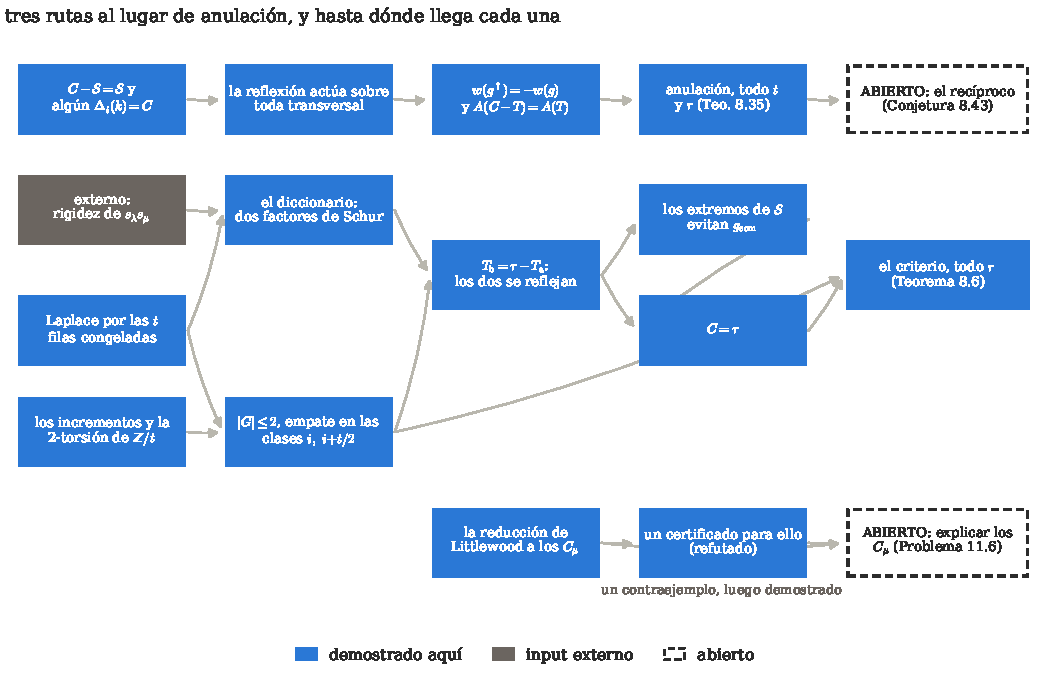
\includegraphics[width=\textwidth]{fig_map_es.pdf}
\caption{Sobre qué se apoya el criterio de la \S\ref{sec:zeros} y qué queda. Las cajas son
enunciados y las flechas dependencias; el color es la columna de estado de la \S\ref{sec:verif} ---
relleno lo demostrado aquí, gris el único apoyo ajeno, discontinuo lo abierto. La rama de arriba es
el argumento extremal de las \S\S\ref{sec:extremal} y \ref{sec:rigidity}; la de abajo es la
reducción de Littlewood, cuyo certificado refuta la Proposición \ref{conj:iso} ---un contraejemplo,
o sea una demostración---, de modo que la rama de abajo ya no toca el criterio sino la cuestión
aparte de explicar los $C_\mu$, que es el Problema \ref{prob:instrument}. Los enunciados van por
nombre y no por número, para que la figura no pueda desfasarse cuando la numeración lo haga.
Calculada por \texttt{anc/fig\_proof.py}.}
\label{fig:map}
\end{figure}

\begin{problem}[los otros tipos clásicos]\label{prob:types}
Todo lo anterior es de tipo $A$. ¿Qué hacen $sp_\lambda(\zt,z,\zb)$, $so_\lambda(\zt,z,\zb)$ y
$o_\lambda(\zt,z,\zb)$? Las factorizaciones de raíces de la unidad se llevaron del tipo $A$ a los
tipos $B$, $C$, $D$ con un argumento uniforme en \cite{AK22} y a los caracteres universales en
\cite{Alb23}; las filas congeladas del bialternante son las mismas en todos los tipos, de modo que el
Lema \ref{lem:L1} y el recuento de exceso dos deberían sobrevivir palabra por palabra, mientras que
el colapso, los Lemas \ref{lem:L4} y \ref{lem:L5}, habría que rehacerlo una vez por tipo. El alfabeto
\eqref{eq:object} es ya un elemento del toro de $O(t+2)$, de modo que los otros tipos no son la misma
función en un punto nuevo sino objetos nuevos, y elegir los correctos es cuestión de criterio dentro
de un programa que no hemos construido nosotros. Sí hemos medido, y lo damos como medición y nada
más. Desarrollando los caracteres universales de Koike--Terada en la base de Schur y evaluando
término a término con el Teorema \ref{thm:main}, sobre $|\lambda|\le12$ para $t\le3$ y
$|\lambda|\le10$ para $t=4,5$, la fracción de formas con $\ell(\lambda)\ge2$ en las que el valor se
anula es netamente mayor para $o_\lambda$ en la componente no identidad que en la identidad ---el
$83.8\%$ con $t=2$ frente al $41.8\%$ con $t=3$, y el $58.8\%$ con $t=4$ frente al $42.1\%$ con
$t=5$---, con $sp_\lambda$ en medio y el caso de Schur el más bajo. El efecto es real y sigue a la
componente, que es lo que cabría esperar de una cancelación entre asociados; pero es cuantitativo y
no le hemos encontrado ley que cubra la tabla entera. Un primer intento de ley, que $o_\lambda$ se
anule para todo
$\ell(\lambda)\ge2$ cuando $t$ es par, es falso: se leyó de una muestra y el barrido sistemático lo
refuta.

La columna $t=2$ de esa comparación es el único caso que sí tiene ley, y es el Lema
\ref{lem:AtoSp}: allí el alfabeto es \eqref{eq:psir} con $r=1$, de modo que $o_\nu$ es igual a
$sp_\nu(z)$, un carácter simpléctico de \emph{rango uno}. Ése se anula idénticamente para
$\ell(\nu)=2$ --- las $36$ formas del rango, sin excepción --- y se pliega para $\ell(\nu)>2$, que es
la razón de que la cifra de $t=2$ sea la que se sale. Lo que queda sin ley es $t$ impar, donde el
alfabeto no tiene la forma \eqref{eq:psir} y el lema no se aplica.

La columna de $sp_\lambda$ en $t=2$, en cambio, sí tiene respuesta, y explica la asimetría de la
tabla en lugar de añadirle una fila. Adjuntar esas mismas dos letras a un carácter universal
\emph{simpléctico} no lo colapsa. Sobre $|\nu|\le8$,
\begin{equation}\label{eq:spbranch}
sp_\nu(W,1,-1)\;=\;\sum_{\gamma\subseteq\nu}c_{\nu/\gamma}\;sp_\gamma(W),
\end{equation}
donde el coeficiente depende de $\nu$ y $\gamma$ solo a través de la forma sesgada $\nu/\gamma$
---$247$ coeficientes sobre $74$ formas sesgadas distintas, sin un solo choque--- y toma únicamente
los valores $0$ y $\pm1$, anulándose siempre que $|\nu/\gamma|$ es impar. Esa es la forma que produce
una regla de ramificación para funciones simplécticas universales, y tales reglas existen
\cite{JJLW24}. Leído contra ella, el Lema \ref{lem:AtoSp} dice que para $o_\nu$ los coeficientes
correspondientes se concentran en $\gamma=\nu$: las dos letras colapsan el carácter ortogonal a un
único carácter simpléctico, y dejan el simpléctico repartido por todo el intervalo bajo $\nu$. La
asimetría de la medición es eso, y no un artefacto de los rangos. Lo que no hemos hecho es
identificar $c_{\nu/\gamma}$, que \eqref{eq:spbranch} convierte en una pregunta sobre caracteres
simplécticos universales sesgados en $(1,-1)$ y en nada más.

La tercera columna se resiste a la misma vía, y por una razón estructural y no accidental. Lo que
resuelve las otras dos es que adjuntar una letra es el mapa de anillos $p_k\mapsto p_k+c^k$, de modo
que $\iota_{1}$ y $\iota_{-1}$ actúan sobre $\Lambda$ y componen. La identidad que traería $so$ al
cuadro, $so_\nu(X)=o_\nu(X,\bar X,1,0,\dots)$ de \cite[(2.13)]{AK25}, relaciona ambos sobre un
alfabeto \emph{duplicado}, y una duplicación no es una adjunción: los $\iota$ no llegan. Así que la
columna $so$ no es una laguna de esfuerzo sino de mecanismo, y la dejamos enunciada como tal.
\end{problem}

\begin{problem}[una Verschiebung que vea un par recíproco]\label{prob:versch}
El operador $\varphi_t$ no tiene nada que decir sobre una letra fuera de una $\zeta$-órbita, que es
la razón estructural de que el Teorema \ref{thm:main} no sea corolario de nada de esa línea, y la
razón de que nuestra demostración descienda al alternante. ¿Existe un operador sobre caracteres
universales, o una factorización de $\varphi_t$ a través de un álgebra mayor, que actúe sobre
alfabetos de la forma (unión de $\zeta$-órbitas) $\cup$ (pares recíprocos)? Por la \S\ref{sec:sharp},
un operador así decidiría (D1) y (D2) de una vez. La discusión de allí sugiere una forma
cuantitativa.

Lo que vuelve bien planteada la pregunta, y no vaga, es que cada mitad tiene ya un formalismo, y no
son el mismo. Las $\zeta$-órbitas son territorio de $\varphi_t$, en la formulación de Albion
\cite{Alb23}. Los alfabetos cerrados por inversión son territorio de las funciones simplécticas y
ortogonales universales, que admiten realizaciones por operadores de vértice de las que se siguen sus
reglas de ramificación \cite{JJLW24}. Nuestro alfabeto es uno de cada, y el Lema \ref{lem:AtoSp} es
el único sitio donde ambos se encuentran: allí la $\zeta$-órbita es $\{1,-1\}$, lo bastante pequeña
como para que adjuntarla sea un par de mapas de letra y no un operador. No conocemos nada que actúe
sobre las dos mitades a la vez, y la pregunta es si los dos formalismos componen.
\end{problem}

\begin{proposition}[el rango es el invariante equivocado]\label{conj:rank}
Sea $A=\zt\cup B$ con $B$ cerrado bajo inversión y disjunto de $\zt$, y sea $\rho(B)$ el rango del
subgrupo de $\CC^{\times}$ generado por $B$. Entonces $\rho(B)=1$ no implica que $s_\lambda(A)$ sea
un producto de caracteres. En $t=2$ y $B=\{z,z^{-1},z^{2},z^{-2}\}$, que tiene $\rho(B)=1$, el valor
en $\lambda=(2)$ tiene una raíz fuera de la circunferencia unidad, y por tanto no admite tal
factorización; lo mismo ocurre con $B=\{z,z^{-1},z^{3},z^{-3}\}$.
\end{proposition}

\begin{proof}
Un producto de caracteres $\chi_k(z)=(z^{k+1}-z^{-k-1})/(z-z^{-1})$ tiene todas sus raíces en la
circunferencia unidad, así que basta exhibir una raíz fuera de ella. Para
$B=\{z,z^{-1},z^{2},z^{-2}\}$ y $\lambda=(2)$ el valor es
$z^{-4}+z^{-3}+z^{-2}+z^{-1}+3+z+z^{2}+z^{3}+z^{4}$. El polinomio de Laurent es invariante bajo
$z\mapsto z^{-1}$, de modo que escribiendo $x=z+z^{-1}$ y usando $z^{k}+z^{-k}\in\ZZ[x]$ queda
\[
x^{4}+x^{3}-3x^{2}-2x+3\;=\;(x-1)\bigl(x^{3}+2x^{2}-x-3\bigr).
\]
La cúbica tiene discriminante
$18\cdot2\cdot(-1)(-3)-4\cdot2^{3}(-3)+2^{2}(-1)^{2}-4(-1)^{3}-27\cdot(-3)^{2}=-31<0$, luego dos de
sus raíces no son reales. Si $|z|=1$, entonces $x=z+z^{-1}=2\cos\theta$ es real; así que para una
raíz no real $x_0$, ninguna de las dos raíces de $z^{2}-x_0z+1=0$ está en la circunferencia unidad, y
las dos son raíces del valor. Luego la factorización es imposible, y el enunciado es exacto y no
numérico.

Sobre $|\lambda|\le8$ el mismo fenómeno ocurre en $17$ de las $62$ formas no nulas, y con
$B=\{z,z^{-1},z^{3},z^{-3}\}$ en $18$; en el mismo rango, $B=\{z,z^{-1}\}$ tiene todas sus raíces en
la circunferencia sin excepción, como exige el Teorema \ref{thm:main}.
\end{proof}

Lo que el rango no ve es cuántas direcciones libres tiene $B$. Un solo par recíproco es una
dirección; $\{z,z^{-1},z^{2},z^{-2}\}$ genera un grupo de rango uno y son dos, y las dos se ven entre
sí. Así que el invariante sobre el que conjeturar no es $\rho(B)$ sino el número de letras
independientes, y con esa lectura el enunciado pasa a ser el que la \S\ref{sec:sharp} ya hace por
otros medios:

\begin{conjecture}[una sola dirección libre]\label{conj:rank2}
Sea $B$ cerrado bajo inversión y disjunto de $\zt$, como en la Proposición \ref{conj:rank}. Entonces
$s_\lambda(\zt\cup B)$ es cero o un producto de caracteres, para toda $\lambda$, si y solo si $B$ es
un único par recíproco. (La alternativa no es decoración: por el Corolario \ref{cor:zero} el valor sí
se anula para alguna $\lambda$ ya con un par, y $0$ no es un producto de caracteres.)
\end{conjecture}

La evidencia a su favor es el Teorema \ref{thm:main} en un sentido y (D1)--(D4) junto con la
Proposición \ref{conj:rank} en el otro: agrandar $B$ destruye el producto, suba o no suba el rango la
ampliación. No tenemos demostración ni mecanismo propuesto, y es precisamente el enunciado que un
argumento del estilo de $\varphi_t$ debería producir.

Esa hipótesis es bajo la que se enuncia la conjetura, y es también la que una forma general tendría
que soltar. El cierre por inversión de $B$ es suficiente
en la evidencia anterior, pero no es necesario para que haya producto. Escribamos $w=-iy$. El segundo
bloque del alfabeto $\{1,-1,y,-y^{-1}\}$ no es cerrado por inversión y, sin embargo,
\begin{equation}\label{eq:scalar}
s_\lambda\big(1,-1,y,-y^{-1}\big)\;=\;i^{\,|\lambda|}\,s_\lambda\big(-i,\,i,\,w,\,w^{-1}\big),
\end{equation}
y el alfabeto de la derecha sí lo es. La hipótesis que llevaría una forma proyectivamente invariante
no es, por tanto, el cierre por inversión de $B$, sino que $A$ sea un múltiplo
escalar de un conjunto cerrado por inversión. Una clase lateral $\zeta\zt$ es ella misma cerrada por
inversión exactamente cuando $\zeta^{2}=\pm1$, que es donde (D3) rompe y donde no.

\begin{problem}[el instrumento para el segundo par]\label{prob:instrument}
La Sección \ref{sec:zeros} reduce la anulación en $r\ge2$ a un enunciado sobre los coeficientes
$C_\mu$ de \eqref{eq:Cmu}, que son sumas con signo de coeficientes de Littlewood. Ese enunciado ya
no es lo que falta: el Teorema \ref{conj:crit} resuelve la anulación, por el argumento extremal de
la \S\ref{sec:rigidity}, que no se cruza con ningún $C_\mu$. Lo que la reducción pide ahora no es
una demostración sino una \emph{explicación} ---por qué se cancelan esas sumas con signo, en los
propios términos de Littlewood--- y sigue sin haber certificado, pues el que propusimos falla por la
Proposición \ref{conj:iso}. Un problema que era un hueco pasa a ser una pregunta por una segunda
demostración, que es mejor problema y más pequeño. El Lema \ref{lem:AtoSp} resuelve la otra mitad de la reducción --- qué
son los valores $o_\nu(A)$ --- y la resuelve simplécticamente: las dos lecturas del alfabeto
concuerdan porque son la misma lectura, pues el álgebra órbita de $D_{r+1}$ es $C_r$ y no la
subálgebra fija $B_r$. Lo que no toca son los coeficientes. Kumari y Stokke \cite{KS26} han dado
reglas de Murnaghan--Nakayama para funciones de Schur simplécticas, ortogonales y ortosimplécticas;
por el Lema \ref{lem:AtoSp} la pertinente aquí es la simpléctica \cite[Teorema 3.4]{KS26}, y no la
ortogonal par \cite[Teorema 3.10]{KS26}. ¿Calcula su recursión los
$C_\mu$? Su regla arrastra un tercer sumando más allá de añadir y quitar tiras de borde, y es el que
ellas mismas señalan como complicado; el \cite[Corolario 3.5]{KS26} muestra que desaparece en cuanto
$\mu_n+1\ge r$, de modo que es un fenómeno de formas poco profundas. Una forma anterior de este
problema preguntaba si ese sumando es el que da cuenta del fallo de la regla de Littlewood fuera de su
rango; el Lema \ref{lem:AtoSp} responde que no, pues el fallo lo llevan las reglas de modificación
simplécticas, que actúan sobre las etiquetas y no dentro de la recursión. Lo que queda son los
coeficientes, y lo que no hemos intentado es si esa recursión los calcula.

Hay un segundo instrumento, y es el que probaríamos primero. Las reglas de ramificación de Frohmader
\cite{Frohmader} calculan $\mathrm{mult}(\pi^{\nu}_{O_n},\pi^{\lambda}_{GL_n})$ como
$\sum_{\mu}c^{\lambda}_{\mu\nu}(O_n)$ sobre las particiones $\mu$ de filas pares, sin restricción de
rango estable y sin regla de modificación. Nuestros $C_\mu$ de \eqref{eq:Cmu} son sumas con signo de
exactamente las multiplicidades que esas reglas calculan, ensambladas por la involución asociada
$\nu\mapsto\nu^{*}$. Así que la pregunta se vuelve concreta: ¿es $C_\mu(\lambda)=0$, en las dos
ramas, una identidad entre coeficientes de Littlewood--Richardson generalizados que las condiciones
de bandera hagan visible? Ésa es una pregunta sobre tablas, que es la forma en la que nos gustaría
verla contestada.
\end{problem}

\begin{problem}[el lugar adicional, en general]\label{prob:extralocus}
¿Tiene el Teorema \ref{thm:extra} análogo para $sp$, $so$ y $o$? Más en general, ¿para qué
especializaciones de las variables libres adquiere el criterio \eqref{eq:AK53} soluciones
adicionales, y puede leerse siempre el lugar adicional en el núcleo de la especialización actuando
sobre el espacio generado por los caracteres universales, como sugiere la Observación
\ref{rem:why}? Si cada tipo adquiere una familia indexada por un elemento de orden dos del retículo
de residuos, el principio es real.

La pregunta necesita fijar la parte libre, y por una razón computada: la familia extra es un
fenómeno del alfabeto \emph{mínimo}. Añádase un segundo par recíproco y desaparece ---sobre
$t=3,4,5,6$ y $|\lambda|\le14$ el lugar pasa a ser exactamente los $t$-núcleos, para el tipo $s$
tanto como para $sp$ y $o$, mientras que con un solo par el tipo $s$ tiene los dos extras del Teorema
\ref{thm:extra} en $t=4$ y uno en $t=6$. (El segundo par se prueba en $z_2=z_1^{2}$, una
especialización, que solo puede crear coincidencias y no eliminarlas, de modo que un recuento de cero
ahí es un recuento de cero.) El análogo para otro tipo hay que buscarlo, por tanto, en la parte libre
mínima \emph{de ese tipo}, una letra de cada clase; comparar tipos con partes libres de tamaños
distintos mide la parte libre, que es lo que hizo nuestro primer intento.

El núcleo es lo que hay que mirar, pero su \emph{presencia} no decide el lugar; lo decide su
tamaño. Dos partes libres del mismo tamaño pueden colapsar ambas la independencia y comportarse de
manera muy distinta. En el lugar recíproco $s_\mu(z,\zb)=\chi_{\mu_1-\mu_2}(z)$ conserva una
graduación, y el lugar extra es la única familia del Teorema \ref{thm:extra}. Sustitúyase el par
por la $\zeta_2$-órbita $(z,-z)$, donde $s_\mu(z,-z)=z^{|\mu|}s_\mu(1,-1)$ conserva sólo $|\mu|$ y
un signo, y sobre $\ell(\lambda)\le2$ el criterio adquiere $28$ soluciones más en $t=2$ y $186$ en
$t=8$, en ninguna familia que sepamos nombrar. El control es el par libre $(z,w)$, que no tiene
núcleo y devuelve los $t$-núcleos y nada más para todo $t\le8$ ---que es \eqref{eq:AK53} misma, de
modo que el control es su teorema y no una medición nuestra. Así que el par recíproco es la
especialización colapsante de núcleo \emph{mínimo}, y
eso, y no la mera existencia de un núcleo, es lo que hace que su lugar extra sea una sola familia.
\end{problem}

\begin{problem}[las fibras, refinadas por el signo]\label{prob:fibres}
El Corolario \ref{cor:fibregf} describe la fibra de la terna de intervalos, y solo eso. El
invariante es $I_t=(d_1,d_2,d_3,\varepsilon_\lambda)$, y el signo corta cada rama todavía más. Su
corte no es contabilidad, y no es ocioso: por la Observación \ref{rem:signsees} el signo ve las
$t-2$ direcciones que la terna no ve, desde $t=3$ ---constante en $(m_i)$ a $v$ fijo en los $107$
huecos de $t=2$, pero solo en $43$ de $62$ en $t=3$ y $26$ de $36$ en $t=4$. ¿Cuál es la
restricción de $\varepsilon_\lambda$ a una rama? La obstrucción para leerla de
\eqref{eq:fibrelattice} está a la vista en \eqref{eq:sign}: $\inv(b_S)$ es un estadístico de la
palabra beta entera, y las coordenadas del retículo parten esa palabra en dos clases distinguidas y
$t-2$ letras libres, de modo que una regla tendría que volver a montar lo que la biyección separa.

Van con él dos huecos menores. La misma descripción para el perfil de tamaño tres debería ser la
misma contabilidad con una clase de tres en lugar de dos de dos; no la hemos escrito. El perfil
degenerado es otra pregunta, porque allí la fibra es el lugar de anulación entero de $\Phi_t$, que
el Corolario \ref{cor:zero} y la Proposición \ref{rem:lattice} describen por otros medios.
\end{problem}

\begin{problem}[un tamiz que conserva un parámetro]\label{prob:sieving}
En $t=2$ el Corolario \ref{cor:enum} es un recuento con signo de $\mathrm{SSYT}(\lambda,4)$, y un
recuento con signo de orden dos es lo que calcula el fenómeno $q=-1$ de Stembridge \cite{Ste94}:
sobre un conjunto que lleva una involución, el valor en $-1$ cuenta los puntos fijos. Ese es el caso
$\#C=2$ del fenómeno de tamiz cíclico de Reiner, Stanton y White \cite{RSW04}, cuyo Teorema 4.3
evalúa la especialización principal $s_\lambda(1,q,\dots,q^{k-1})$ en una raíz primitiva $d$-ésima
de la unidad en términos del $d$-núcleo y el $d$-cociente de $\lambda$ ---los dos invariantes que
sostienen también el Teorema \ref{thm:main}--- y que Lee y Oh \cite{LO22} han extendido después a
formas sesgadas. Toda evaluación de esa línea es en un \emph{número}, como un enunciado de tamiz
exige: allí el alfabeto es la progresión geométrica $1,q,\dots,q^{k-1}$ especializada en una raíz de
la unidad, no una órbita llana, y no queda nada libre. La nuestra no es de esa clase ---el par
recíproco conserva $z$, y \eqref{eq:main} es una fórmula de producto en él. ¿Hay una acción cíclica
sobre $\mathrm{SSYT}(\lambda,t+2)$, y un $q$-análogo de $\Phi_t$, cuyo valor en una raíz $t$-ésima
de la unidad cuente puntos fijos refinados por $m_{t+1}-m_{t+2}$? El caso $\#C=2$ es por donde mirar
primero, y allí la involución que un enunciado así necesitaría ya existe: la \S\ref{sec:enum} la
ensambla.

Planteada así, la pregunta tiene nombre. Los enunciados de cribado que conservan un estadístico
adicional se estudian por derecho propio ---Ahlbach y Swanson \cite{AS18} refinan el cribado cíclico
sobre palabras fijando el tipo de descenso cíclico junto al índice mayor--- y la forma de dos
variables, en la que una segunda graduación lleva una segunda acción, es el cribado \emph{bicíclico}
de Barcelo, Reiner y Stanton \cite{BRS08}. Sobre tablas semiestándar en particular, Oh y Park
\cite{OP19} construyen una acción cíclica a partir de la estructura de cristal cuyo polinomio de
cribado es $q^{-\kappa(\lambda)}s_\lambda(1,q,\dots,q^{n-1})$ ---la mitad congelada de nuestro
alfabeto, evaluada exactamente como un enunciado de cribado exige--- y obtienen un enunciado
bicíclico para los ganchos; Alexandersson, Kantarc\i{} O\u{g}uz y Linusson \cite{AKL21} hacen lo
mismo bajo promoción para varias familias de formas. Ninguno de ellos conserva una variable
\emph{libre}, que es lo que \eqref{eq:object} sí hace y lo que vuelve distinta la pregunta de aquí,
pero entre todos dicen qué aspecto debería tener una respuesta. La forma afilada es entonces: ¿lleva
cada fibra de peso $z$ fijo de $\mathrm{SSYT}(\lambda,t+2)$ un cribado cíclico propio?

La mitad de existencia de la pregunta es decidible sin exhibir la acción. Alexandersson y Amini
\cite{AA19} dan un criterio necesario y suficiente para que exista una acción cíclica que realice un
polinomio de tamiz dado: para todo $d\mid t$, el valor en $\omega^d$ debe ser
$\sum_{j\mid d}j\,c_j$ con todos los $c_j$ enteros no negativos, y los $c_j$ ---los números de
órbitas de cada tamaño--- se calculan entonces por triangularidad. Aplicado al candidato que sugiere
el propio alfabeto, $F(q,z)=s_\lambda(1,q,\dots,q^{t-1},z,z^{-1})$, cuya graduación en $z$ es ya el
refinamiento que se pide, el criterio se cumple para casi toda pieza graduada en los rangos que
alcanzamos; pero también para un refinamiento deliberadamente equivocado, graduando por
$m_{t+1}+m_{t+2}$, que pasa al mismo ritmo. A esos tamaños el criterio no discrimina, y damos el
intento como evidencia en ninguna de las dos direcciones.
\end{problem}

Una laguna más estrecha queda registrada donde surge y no aquí, con la misma forma que los problemas
anteriores y el mismo significado ---algo que querríamos saber y no hemos resuelto---: la involución
de la \S\ref{sec:enum} queda ensamblada en $t=2$ y en ningún otro sitio, porque la Proposición
\ref{rem:involution} es un enunciado sobre una palabra y esa palabra es la de $t=2$. La
distinción que mantenemos en todo el texto es entre una \emph{conjetura}, que es un enunciado que
creemos y hemos testado, y un \emph{problema}, que no es una afirmación en absoluto.

Tomados juntos, los problemas dicen dónde creemos que el objeto deja de ser nuestro. La evaluación
está completa y el alfabeto es mínimo, así que lo que queda no es más de lo mismo: es si los dos
formalismos que se reparten las dos mitades de \eqref{eq:object} componen, si un enunciado de tamiz
puede conservar una variable, y qué hacen los coeficientes $C_\mu$ una vez retirado el certificado
que habíamos propuesto para ellos. De los tres, el último es el que el artículo necesita y el primero
es el que preferiríamos ver contestado.

Conviene cerrar donde empezamos. La introducción nombró dos razones para que la evaluación de un
carácter colapse ---que el alfabeto sea una órbita, y que sea cerrado por inversión--- y observó que
ningún alfabeto había llevado una de cada. Éste sí, y las dos razones se comportan en él de manera
muy distinta. La mitad de la órbita está agotada: el Teorema \ref{thm:main} la evalúa en forma
cerrada para todo $t$, y el Teorema \ref{thm:extra} muestra que, dentro del problema de independencia
para formas de dos filas, exactamente una familia más se comporta así. La mitad de la inversión no lo
está: la letra $-1$ lleva el alfabeto a la componente no identidad de un grupo ortogonal, y eso ha
bastado para decir bastante sobre \emph{dónde} se anula el carácter ---el Teorema \ref{conj:crit} lo
resuelve en $t=2$ para cualquier número de pares, y el Teorema \ref{thm:suff} da una implicación para
todo $t$ y todo $r$---, pero no nos ha dicho qué \emph{es} el carácter allí para más de un par, y la
otra implicación es la Conjetura \ref{conj:general}. El valor no deja nunca de ser un valor de
carácter: es $s_\lambda$ evaluado en un elemento del toro en todo momento. Lo que deja de valer,
pasado un par, es que su expansión simpléctica plegada sea siempre un carácter genuino: a partir de
dos pares aparecen ejemplos genuinamente virtuales. Eso es un enunciado sobre la expansión, no sobre
el objeto. Lo que el artículo entrega es más pequeño que cualquiera de las dos mitades y más portátil: una
forma cerrada que lleva su signo, lo que convierte a esta familia en un caso de prueba para cualquier
implementación de caracteres torcidos o universales; un test de anulación que cuesta dos restas sobre
el conjunto beta; y una enumeración en la que el parámetro sigue libre. Quien
busque el alfabeto siguiente habrá de buscar el que deje la segunda razón tan completa como aquí ha
quedado la primera; a la vista de la \S\ref{sec:sharp}, no lo encontrará añadiendo letras a éste.

\subsection*{Agradecimientos}
Este artículo existe porque Arvind Ayyer preguntó si el caso de rango uno se generaliza a $t$
arbitrario con la variable libre simbólica. La pregunta era mejor que la nota que la provocó. Le
agradecemos tanto la pregunta como la correspondencia que siguió. La Observación \ref{rem:core} existe
porque Nishu Kumari preguntó si la condición $n_i(\lambda)=0$ podía formularse en términos del
$t$-núcleo; también confirmó la lectura de \cite[Teorema 5.3]{AK25} de la \S\ref{sec:independence}, y
fue un apunte suyo el que nos envió a \cite[\S3]{AK25}, donde esperaba el Lema \ref{lem:AtoSp}; se lo
agradecemos. La involución de la
\S\ref{sec:enum} está montada a partir de tres lemas de su tesis \cite{KumariThesis}, y en ese
sentido también es suya.

Hay una tercera deuda, y es con una herramienta y no con una conversación. La prueba del Teorema
\ref{thm:suff} depende de poder reflejar un conjunto beta dentro de un determinante sin desarrollar
nada, y la manera de hacerlo --- escalar cada fila por una potencia para mandar $x_i$ a $\bar x_i$ y
luego invertir un bloque de columnas --- es la maniobra de Ayyer y Behrend \cite[\S3]{AB19}, usada del
lado de las raíces de la unidad por Albion \cite{Alb23,Alb25}. La adoptamos porque es a todas luces
el instrumento adecuado para un alfabeto cerrado por inversión, y la mantuvimos porque resultó ser
más robusta que el contexto para el que se escribió: en ningún momento usa que la reflexión se
aplique al alfabeto entero, así que funciona igual sobre una parte de él. Todo lo que la
\S\ref{sec:zeros} dice sobre $t\ge4$ se apoya en eso.

\subsection*{Código, datos y declaración}
Todo cálculo citado en este artículo lo realiza un script con nombre, distribuido como fichero
adjunto, y todo número citado lo reproduce una ejecución archivada de alguno de ellos; la
\S\ref{sec:verif} tabula qué script responde por qué afirmación. Los mismos scripts y la misma salida
están también en \url{https://github.com/karlesmarin/schur-orbit-and-reciprocal-pair}. Se ha usado IA generativa (Claude,
Anthropic) como asistente de investigación durante todo el trabajo: para la búsqueda bibliográfica,
para escribir y comprobar el código adjunto, y sobre la prosa. Las matemáticas, y la responsabilidad
sobre ellas, son del autor.

%======================================================================
\begin{thebibliography}{AAAA}

\bibitem[FG86]{FG86} A.~Federgruen y H.~Groenevelt, \emph{The greedy procedure for resource
allocation problems: necessary and sufficient conditions for optimality}, Oper. Res. \textbf{34}
(1986), no.~6, 909--918.

\bibitem[HK16]{HK16} A.~Hanany y R.~Kalveks, \emph{Quiver theories for moduli spaces of classical
group nilpotent orbits}, arXiv:1601.04020.

\bibitem[IK88]{IK88} T.~Ibaraki y N.~Katoh, \emph{Resource Allocation Problems: Algorithmic
Approaches}, MIT Press, Cambridge MA, 1988.

\bibitem[PvW08]{PvW} K.~Purbhoo y S.~van Willigenburg, \emph{On tensor products of polynomial
representations}, Canad. Math. Bull. \textbf{51} (2008), no.~4, 584--592; arXiv:0706.3251.

\bibitem[Raj04]{Rajan} C.~S.~Rajan, \emph{Unique decomposition of tensor products of irreducible
representations of simple algebraic groups}, Ann. of Math. (2) \textbf{160} (2004), no.~2, 683--704.

\bibitem[RGST05]{TropCramer} J.~Richter-Gebert, B.~Sturmfels y T.~Theobald, \emph{First steps in
tropical geometry}, en: Idempotent Mathematics and Mathematical Physics, Contemp. Math. \textbf{377},
Amer. Math. Soc., 2005, pp.~289--317.


\bibitem[Alb23]{Alb23} S.~P.~Albion, \emph{Universal characters twisted by roots of unity},
Algebraic Combinatorics \textbf{6} (2023), 1653--1676; arXiv:2212.07343.

\bibitem[Alb25]{Alb25} S.~P.~Albion, \emph{Character factorisations, $z$-asymmetric partitions and
plethysm}, en prensa en Combinatorial Theory; arXiv:2501.18520.

\bibitem[AS18]{AS18} C.~Ahlbach y J.~P.~Swanson, \emph{Refined cyclic sieving on words for the
major index statistic}, European J. Combin. \textbf{73} (2018), 37--60; arXiv:1706.08631.

\bibitem[BRS08]{BRS08} H.~Barcelo, V.~Reiner y D.~Stanton, \emph{Bimahonian distributions},
J. London Math. Soc. (2) \textbf{77} (2008), 627--646; arXiv:math/0703479.

\bibitem[OP19]{OP19} Y.-T.~Oh y E.~Park, \emph{Crystals, semistandard tableaux and cyclic sieving
phenomenon}, Electron. J. Combin. \textbf{26} (2019), no.~4, \#P4.39; arXiv:1906.07420.

\bibitem[AKL21]{AKL21} P.~Alexandersson, E.~Kantarc\i{} O\u{g}uz y S.~Linusson, \emph{Promotion and
cyclic sieving on families of SSYT}, Ark. Mat. \textbf{59} (2021), 247--274; arXiv:2007.10478.

\bibitem[AA19]{AA19} P.~Alexandersson y N.~Amini, \emph{The cone of cyclic sieving
phenomena}, Discrete Math. \textbf{342} (2019), n.º~6, 1581--1601; arXiv:1804.01447.

\bibitem[AB19]{AB19} A.~Ayyer y R.~E.~Behrend, \emph{Factorization theorems for classical group
characters, with applications to alternating sign matrices and plane partitions}, J. Combin. Theory
Ser.~A \textbf{165} (2019), 78--105; arXiv:1804.04514.

\bibitem[AK22]{AK22} A.~Ayyer y N.~Kumari, \emph{Factorization of classical characters twisted by
roots of unity}, J. Algebra \textbf{609} (2022), 437--483; arXiv:2109.11310.

\bibitem[AK25]{AK25} A.~Ayyer y N.~Kumari, \emph{Further results for classical and universal
characters twisted by roots of unity}, J. Algebraic Combin. \textbf{63} (2026), Paper No.~2, 32 pp.;
arXiv:2501.00275.

\bibitem[CK09]{CK09} M.~Ciucu y C.~Krattenthaler, \emph{A factorization theorem for classical
group characters, with applications to plane partitions and rhombus tilings}, in: Advances in
Combinatorial Mathematics, Springer, Berlin, 2009.

\bibitem[GKS90]{GKS90} F.~Garvan, D.~Kim y D.~Stanton, \emph{Cranks and $t$-cores},
Invent. Math. \textbf{101} (1990), no.~1, 1--18.

\bibitem[HI24]{HI24} M.~Hidaka y M.~Itoh, \emph{The Schur polynomials in all primitive $n$th roots
of unity}, J. Combin. Theory Ser.~A \textbf{218} (2026), Paper No.~106107; arXiv:2403.10817.

\bibitem[Jan73]{Jantzen} J.~C.~Jantzen, \emph{Darstellungen halbeinfacher algebraischer Gruppen},
Bonner Math. Schriften \textbf{67} (1973).

\bibitem[Kar22]{Kar22} C.~Karmakar, \emph{Character factorizations for representations of
$GL(n,\CC)$}, arXiv:2210.03544.

\bibitem[Kar24]{Kar24} C.~Karmakar, \emph{Character values at elements of order $2$},
Proc. Indian Acad. Sci. Math. Sci. \textbf{135} (2025), no.~2, Paper No.~41; arXiv:2412.17324.

\bibitem[Mar26]{Mar26} C.~Mar\'in, \emph{Schur functions at $(1,-1,t,t^{-1})$: a closed form on the
non-identity component of $O(4)$}, preprint, 2026; \texttt{doi:10.5281/zenodo.21463000}.

\bibitem[JJLW24]{JJLW24} Z.~Jin, N.~Jing, Z.~Li y D.~Wang, \emph{Universal symplectic/orthogonal
functions and general branching rules}, arXiv:2209.00767.

\bibitem[KLP09]{KLP} S.~Kumar, G.~Lusztig y D.~Prasad, \emph{Characters of simply-laced
nonconnected groups versus characters of nonsimply-laced connected groups}, Contemp. Math.
\textbf{478} (2009), 99--101; arXiv:math/0701615.

\bibitem[KT99]{KT99} A.~Knutson y T.~Tao, \emph{The honeycomb model of $GL_n(\CC)$ tensor
products I: proof of the saturation conjecture}, J. Amer. Math. Soc. \textbf{12} (1999), no.~4,
1055--1090.

\bibitem[Kum24]{Kum24} N.~Kumari, \emph{Factorization of classical characters twisted by roots of
unity: II}, J. Pure Appl. Algebra \textbf{228} (2024), no.~11, 107714; arXiv:2212.12477.

\bibitem[KumT]{KumariThesis} N.~Kumari, \emph{Characters of classical groups twisted by roots of
unity}, tesis doctoral, Indian Institute of Science, Bangalore, 2023.

\bibitem[Lec09]{Lec09} C.~Lecouvey, \emph{Parabolic Kazhdan--Lusztig polynomials, plethysm and
generalized Hall--Littlewood functions for classical types}, European J. Combin. \textbf{30} (2009),
no.~1, 157--191.

\bibitem[LR34]{LR34} D.~E.~Littlewood y A.~R.~Richardson, \emph{Immanants of some special
matrices}, Q. J. Math. \textbf{os-5} (1934), no.~1, 269--282.

\bibitem[LLT97]{LLT97} A.~Lascoux, B.~Leclerc y J.-Y.~Thibon, \emph{Ribbon tableaux,
Hall--Littlewood functions, quantum affine algebras and unipotent varieties}, J. Math. Phys.
\textbf{38} (1997), no.~2, 1041--1068.

\bibitem[LO22]{LO22} S.-Y.~Lee and Y.-T.~Oh, \emph{Skew Schur polynomials and cyclic sieving
phenomenon}, Electron. J. Combin. \textbf{29} (2022), no.~4, Paper 4.6; arXiv:2112.12394.

\bibitem[Mac95]{Mac95} I.~G.~Macdonald, \emph{Symmetric Functions and Hall Polynomials}, second
edition, Oxford University Press, 1995.

\bibitem[RSW04]{RSW04} V.~Reiner, D.~Stanton y D.~White, \emph{The cyclic sieving phenomenon},
J. Combin. Theory Ser. A \textbf{108} (2004), no.~1, 17--50.

\bibitem[Ste94]{Ste94} J.~R.~Stembridge, \emph{On minuscule representations, plane partitions and
involutions in complex Lie groups}, Duke Math. J. \textbf{73} (1994), no.~2, 469--490.

\bibitem[Oka98]{Oka98} S.~Okada, \emph{Applications of minor summation formulas to
rectangular-shaped representations of classical groups}, J. Algebra \textbf{205} (1998), no.~2,
337--367.

\bibitem[Pra16]{Pra16} D.~Prasad, \emph{A character relationship on $GL_n(\CC)$}, Israel J. Math.
\textbf{211} (2016), no.~1, 257--270.

\bibitem[AF20]{AF20} A.~Ayyer e I.~Fischer, \emph{Bijective proofs of skew Schur polynomial
factorizations}, J. Combin. Theory Ser.~A \textbf{174} (2020), 105241; arXiv:1905.05226.

\bibitem[Doc]{Doc} Para el nombre y la familia de identidades que lo rodea (Cassini, Catalan,
d'Ocagne, Vajda) véase p.\,ej.\ M.~Bunder y J.~Tonien, \emph{Cassini, d'Ocagne and Vajda identities
for $n$-step Fibonacci numbers}, arXiv:2201.06269.

\bibitem[Eis07]{Eis07} T.~Eisenk\"olbl, \emph{A Schur function identity related to the
$(-1)$-enumeration of self-complementary plane partitions}, J. Combin. Theory Ser.~A \textbf{115}
(2008), 199--212; arXiv:math/0602401.

\bibitem[FJKW05]{FJKW05} B.~Fauser, P.~D.~Jarvis, R.~C.~King y B.~G.~Wybourne, \emph{New branching
rules induced by plethysm}, J. Phys. A \textbf{39} (2006), 2611--2655; arXiv:math-ph/0508034.

\bibitem[Gav99]{Gav99} F.~Gavarini, \emph{A Brauer algebra-theoretic proof of Littlewood's
restriction rules}, J. Algebra \textbf{212} (1999), 240--271.

\bibitem[EW04]{EW04} T.~J.~Enright y J.~F.~Willenbring, \emph{Hilbert series, Howe duality and
branching for classical groups}, Ann. of Math. \textbf{159} (2004), 337--375.

\bibitem[New51]{New51} M.~J.~Newell, \emph{Modification rules for the orthogonal and symplectic
groups}, Proc. Roy. Irish Acad. Sect. A \textbf{54} (1951), 153--163.

\bibitem[Sun90]{Sun90} S.~Sundaram, \emph{Tableaux in the representation theory of the classical Lie
groups}, en \emph{Invariant Theory and Tableaux} (Minneapolis, MN, 1988), IMA Vol. Math. Appl.
\textbf{19}, 191--225, Springer-Verlag, Nueva York, 1990.

\bibitem[IOTZ06]{IOTZ06} M.~Ishikawa, S.~Okada, H.~Tagawa y J.~Zeng, \emph{Generalizations of
Cauchy's determinant and Schur's Pfaffian}, Adv. in Appl. Math. \textbf{36} (2006), 251--287.

\bibitem[Fro25]{Frohmader} A.~Frohmader, \emph{Graded multiplicities in the Kostant--Rallis
setting}, arXiv:2312.11295.

\bibitem[Kra05]{KratADCC} C.~Krattenthaler, \emph{Advanced determinant calculus: a complement},
Linear Algebra Appl. \textbf{411} (2005), 68--166; arXiv:math/0503507.

\bibitem[Kin71]{King71} R.~C.~King, \emph{Modification rules and products of irreducible
representations of the unitary, orthogonal, and symplectic groups}, J. Math. Phys. \textbf{12}
(1971), 1588--1598.

\bibitem[KT87]{KT87} K.~Koike e I.~Terada, \emph{Young-diagrammatic methods for the representation
theory of the classical groups of type $B_n$, $C_n$, $D_n$}, J. Algebra \textbf{107} (1987),
466--511.

\bibitem[KS26]{KS26} N.~Kumari y A.~Stokke, \emph{Murnaghan--Nakayama rules for symplectic,
orthogonal and orthosymplectic Schur functions}, Discrete Math. \textbf{349} (2026), no.~2, Paper
No.~114741; arXiv:2411.11447.

\bibitem[Kup02]{Kup02} G.~Kuperberg, \emph{Symmetry classes of alternating-sign matrices under one
roof}, Ann. of Math. (2) \textbf{156} (2002), 835--866.

\bibitem[Lit50]{Lit50} D.~E.~Littlewood, \emph{The Theory of Group Characters and Matrix
Representations of Groups}, 2.\textsuperscript{a} ed., Oxford University Press, 1950.

\bibitem[SK23]{SK23} V.~Sathish Kumar, \emph{Flagged skew Schur polynomials twisted by roots of
unity}, arXiv:2306.10289.

\bibitem[Sta86]{Sta86} R.~P.~Stanley, \emph{Symmetries of plane partitions}, J. Combin. Theory
Ser.~A \textbf{43} (1986), 103--113.

\end{thebibliography}

\end{document}
"
% Van los dos aquí, y no en un segundo fichero, a propósito: un fuente duplicado diverge en silencio
% y ninguna compilación falla nunca por ello.
\ifdefined\LONGABS
Sea $\zt=\{1,\zeta,\dots,\zeta^{t-1}\}$ el conjunto completo de las raíces $t$-ésimas de la unidad y
sea $(z,z^{-1})$ un par recíproco libre. Evaluamos $s_\lambda(\zt,z,z^{-1})$ para todo $t\ge2$ y toda
partición $\lambda$ con a lo sumo $t+2$ partes, y sin ninguna hipótesis sobre su forma ni sobre su
tamaño: es un producto con signo de
exactamente tres factores sobre un denominador fijo, o cero, y los tres argumentos se leen del
perfil de residuos y del $t$-cociente de $\lambda$. Equivalentemente, y sin ninguna exponencial a la vista, es un cociente de
caracteres $\mathfrak{sl}_2$: un producto triple sobre el cuadrado de uno. Lo que la identidad deja a
la vista es una estructura, y la estructura es la parte que esperamos que la sobreviva: todo lo que
esta evaluación puede ver de $\lambda$ es un perfil de residuos, una terna de intervalos y un signo, y
aislamos ese dato como un \emph{invariante de la evaluación}. El valor factoriza a través de él, y es
completo ---dos particiones de cualesquiera tamaños que compartan el invariante comparten el valor---,
de modo que una partición arbitrariamente grande queda comprimida a tres enteros y un signo.
La demostración es un
desarrollo de Laplace a lo largo de las $t$ filas
congeladas del bialternante junto con un lema de cancelación en el grupo simétrico, y da el signo,
que es el signo de ordenación ya presente en la evaluación de Littlewood de $s_\lambda(\zt)$ y que
damos también en forma cerrada en la notación de Ayyer y Kumari. Se
registran tres consecuencias. Primera, un criterio de anulación: el carácter se anula exactamente
cuando alguna clase de residuos módulo $t$ es vacía, o cuando dos clases distinguidas son
concéntricas como intervalos ---y el segundo caso solo ocurre para $t$ par, de modo que en $t$ impar
una clase vacía es la única forma de anularse. Segunda, una extensión de un criterio de independencia reciente de
Ayyer y Kumari: su teorema determina cuándo un carácter es independiente de las variables por las que
está torcido, y mostramos que, para formas de dos filas, en el lugar recíproco el criterio adquiere exactamente una familia
adicional, que clasificamos por su núcleo y su cociente. Su teorema está enunciado para variables
libres y un par recíproco no lo es, de modo que el lugar queda fuera de sus hipótesis y no en contra
de ellas, y lo que determinamos es en qué se convierte allí el criterio. Tercera, una lectura enumerativa: la identidad es una fórmula de producto para un recuento de
tablas semiestándar pesado por raíces de la unidad en el que un parámetro sigue libre, y en $t=2$ es
una $(-1)$-enumeración de particiones planas en una caja refinada por ese parámetro; una
demostración de ella que invierta el signo ha de transportar ese parámetro, y aportamos la mitad de
la cancelación que atraviesa la partición del alfabeto. Por último
mostramos que la factorización está aislada: falla bajo cada una de las cuatro deformaciones del
alfabeto ---más pares recíprocos, más variables en la órbita, la órbita sustituida por una clase
lateral, el par recíproco sustituido por un par libre--- y una sola lectura de la demostración
explica los cuatro fallos a la vez.

Lo que sí sobrevive a la primera de esas deformaciones es el \emph{lugar de anulación}, y de él trata
la última sección. Escribamos $\Psi_r=s_\lambda(1,-1,z_1,z_1^{-1},\dots,z_r,z_r^{-1})$. Hay dos
condiciones que hacen que $\Psi_r$ se anule: que el conjunto beta de $\lambda$ tenga paridad
constante, y que $\lambda$ sea autocomplementaria de anchura impar. \emph{Esa} implicación la
demostramos para todo $r$ y toda $\lambda$, y no reclamamos nada por ella: es un corolario corto de la
identidad de complementación sobre una familia de índices que Ayyer y Behrend ya destacan, y en el
mismo alfabeto \emph{sin} la letra $-1$ sus teoremas hacen que esas mismas formas factoricen ---quien
decide es el determinante del alfabeto. El contenido nuevo es el \emph{recíproco}, que no se anula
nada más, y lo demostramos para todo $r$ y toda $\lambda$ por un argumento extremal en la filtración
por grados cuyo único apoyo ajeno es un teorema de rigidez para productos de polinomios de Schur.
Leído sobre el grupo y no sobre el alfabeto, ese criterio clasifica exactamente los $GL(N)$-módulos
polinómicos irreducibles cuya restricción a $O(N)$ es estable bajo el giro por el determinante. El
mismo argumento resuelve una segunda línea del plano $(t,r)$, y la resuelve del todo y sin ningún
apoyo ajeno: para todo $t$ \emph{impar} y todo $r$, el carácter se anula si y solo si falta una clase
de residuos del conjunto beta, de modo que la rama concéntrica es un fenómeno exclusivo de $t$ par.
Eso deja $t\ge4$ par y $r\ge2$ como la única región donde el lugar de anulación queda abierto, y allí
dejamos escrita la condición necesaria que el argumento sí da. Un solo par resulta además no ser
típico: allí $\Psi_1$ es un carácter genuino salvo
signo, de modo que una única especialización de orden dos decide si se anula, y a partir de dos pares
eso deja de ser cierto.
\else
Sea $\zt$ el conjunto completo de las raíces $t$-ésimas de la unidad. Adjuntar $r$ pares recíprocos
libres da una familia de alfabetos con dos parámetros; resolvemos tres partes de ella.

En $r=1$, para todo $t\ge2$ y toda $\lambda$ con a lo sumo $t+2$ partes, $s_\lambda(\zt,z,z^{-1})$ es
un producto con signo de exactamente tres factores sobre un denominador fijo, o cero, con los
argumentos leídos del núcleo y del cociente. Lo que ve de $\lambda$ es un multiconjunto de tres enteros y un
signo, y exactamente eso: dos particiones de cualesquiera tamaños comparten un valor no
nulo si y solo si coinciden en ese dato. La demostración es un desarrollo de Laplace a lo largo de
las $t$ filas congeladas con un lema de cancelación, y da el signo, que ya es el de Littlewood.

En $t=2$ y todo $r$, $s_\lambda(1,-1,z_1^{\pm1},\dots,z_r^{\pm1})$ se anula exactamente cuando el
conjunto beta tiene paridad constante o $\lambda$ es autocomplementaria de anchura impar; esa
dirección es un corolario de la complementación sobre una familia de índices que Ayyer y Behrend
destacan, y el recíproco un argumento extremal en la filtración por grados, módulo un teorema de
rigidez para productos de Schur.
Equivalentemente: exactamente esos $V_\lambda$ restringen a $O(N,\mathbb{C})$ de forma estable por $\det$.
En $t$ impar y todo $r$ se anula exactamente cuando falta una clase
de residuos, sin coste externo alguno. Y para todo $t$ y todo $r$, una
reflexión de la \emph{parte de exceso} del conjunto beta con un incremento que da en su centro
fuerza la anulación.

Tres consecuencias de lo primero. Un criterio de anulación: una clase de residuos vacía, o dos clases
distinguidas concéntricas como intervalos, lo segundo solo para $t$ par. Una extensión de un criterio
de independencia de Ayyer--Kumari: en el lugar recíproco adquiere una familia más, clasificada por
núcleo y cociente. Y en $t=2$ una $(-1)$-enumeración de particiones planas en una caja refinada por un
parámetro que sigue libre. La factorización está aislada: falla bajo cada una de cuatro deformaciones
del alfabeto, y por una sola razón.
\fi
\end{abstract}

\maketitle

%======================================================================
\section{Introducción}

Un polinomio de Schur es un carácter. Escrito $s_\lambda(x_1,\dots,x_n)$, es la traza de una matriz
de valores propios $x_1,\dots,x_n$ actuando sobre la representación irreducible de $GL_n$ etiquetada
por $\lambda$, y leerlo así convierte cada elección de las variables en una pregunta sobre un
elemento de un grupo y no sobre un polinomio. Dos de esas preguntas son tan antiguas como la materia.
En la identidad, con todos los $x_i=1$, la traza es una dimensión y crece con $\lambda$. En un
elemento de orden finito deja de crecer: si las variables recorren una órbita completa de raíces
$t$-ésimas de la unidad, el valor es $0$ o $\pm1$, y cuál de los tres depende de una propiedad de
divisibilidad de $\lambda$ y no de su tamaño. Algo que podía ser arbitrariamente grande queda
comprimido a casi nada, y la razón es aritmética. Todo lo que sigue trata de hasta dónde alcanza esa
compresión: cuánto alfabeto puede añadirse antes de que el colapso se detenga, y qué sobrevive
exactamente de una partición cuando no se detiene.

Se conocen dos razones estructurales para un colapso así, y cada una ha dado su propia literatura. La
primera es que el alfabeto sea una \emph{órbita}: un conjunto completo de raíces $t$-ésimas de la
unidad es la lista de valores propios de un elemento de orden $t$, y las órbitas son lo que los
operadores de esa línea están hechos para ver. La segunda es que el alfabeto sea \emph{cerrado por
$x\mapsto x^{-1}$}: una lista así es el espectro de una matriz ortogonal, de modo que el carácter de
$GL$ se está restringiendo a un grupo más pequeño, y es la restricción la que factoriza. Las dos
razones son independientes entre sí, y también lo son las dos literaturas; los párrafos que siguen
recorren cada una, y la \S\ref{sec:sharp} muestra que ninguna sobrevive si se la empuja al terreno de
la otra. El alfabeto de este artículo es el más pequeño que lleva una razón de cada clase.

La Figura \ref{fig:thread} es el artículo leído como una sola cadena: cada respuesta es lo que
levanta la pregunta siguiente, y cada perla lleva la sección que la resuelve. La Figura
\ref{fig:alphabet} dibuja el alfabeto mismo, que es el único objeto del que trata todo lo demás.

\begin{figure}[!ht]
\centering
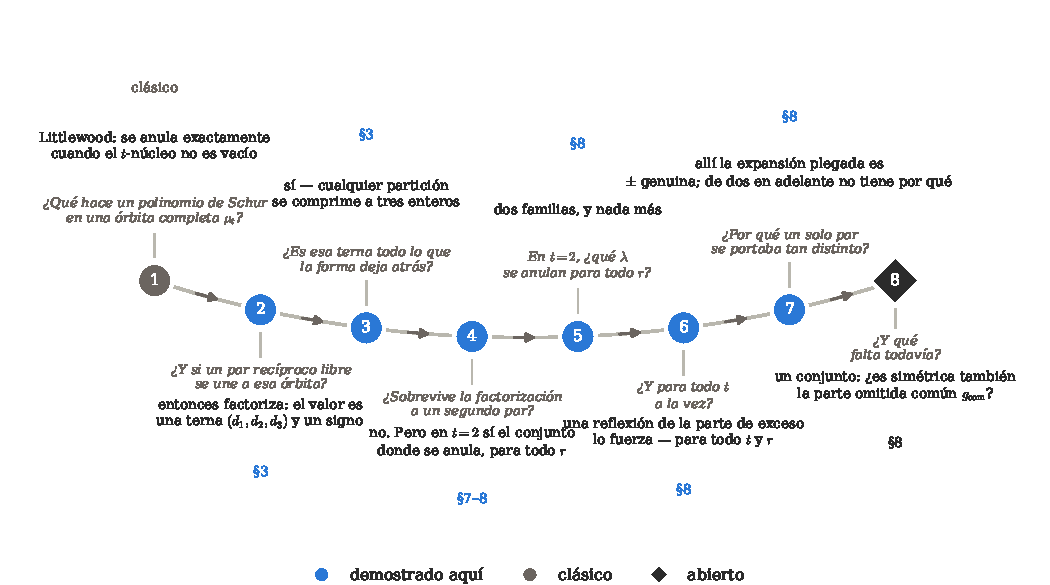
\includegraphics[width=\textwidth]{fig_thread_es.pdf}
\caption{El artículo como un solo hilo. Cada pregunta la responde la perla que tiene debajo, y
cada respuesta es lo que hace que la siguiente pregunta sea la natural: la órbita pide el par
libre, la factorización pide la terna, la terna pide el segundo par, y el segundo par convierte una
fórmula en un lugar. El color distingue lo clásico, lo demostrado aquí y lo que queda abierto, y la
etiqueta bajo cada respuesta es la sección que la resuelve. Dibujada por
\texttt{anc/fig\_intro.py}.}
\label{fig:thread}
\end{figure}

\begin{figure}[!ht]
\centering
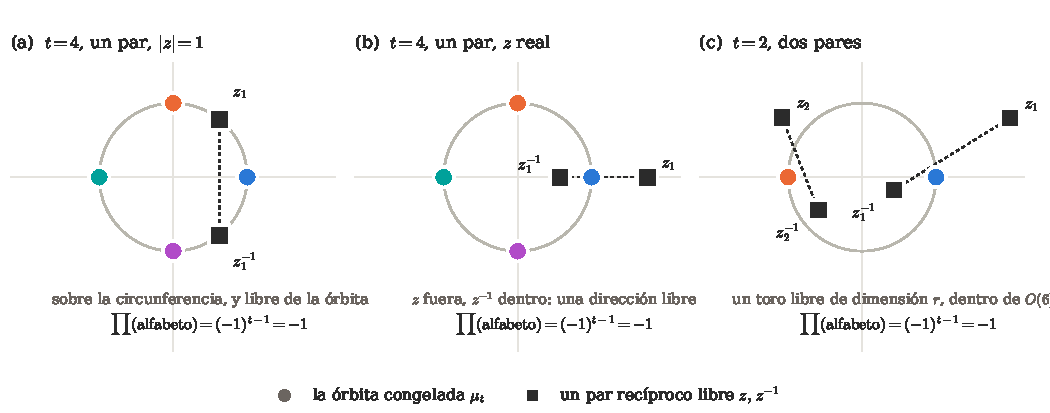
\includegraphics[width=\textwidth]{fig_alphabet_es.pdf}
\caption{El alfabeto, en el plano complejo. La órbita $\mu_t$ está congelada ---un $t$-gono
regular sobre la circunferencia unidad, coloreado por residuo--- y cada par recíproco es una
dirección compleja libre, dibujada unida por un segmento discontinuo. \emph{(a)} el par puede estar
sobre la circunferencia; es una variable libre y no parte de la órbita, y salvo para finitos $z$ no
toca $\mu_t$, que es la razón de que un operador hecho para órbitas de $\zeta$ no tenga nada que
decir de él. \emph{(b)} fuera de la circunferencia, $z$ por fuera y $z^{-1}$ por dentro. \emph{(c)}
$r$ pares dan un toro libre de dimensión $r$. En todos los casos el alfabeto es cerrado por
inversión, así que es la lista de valores propios de un elemento de $O(N,\CC)$ ---el panel (b)
muestra por qué el grupo tiene que ser el complejo--- y el producto de sus letras vale $\zeta^{t(t-1)/2}=(-1)^{t-1}$: para $t$ par esa matriz
está en la componente no identidad. Calculada por \texttt{anc/fig\_intro.py}.}
\label{fig:alphabet}
\end{figure}


Una partición puede ser arbitrariamente grande, y un alfabeto de $N=t+2$ letras sólo alcanza a ver
una parte de ella. Este artículo resuelve, para un alfabeto, exactamente cuánta. El conjunto
completo de las raíces $t$-ésimas de la unidad junto con un par recíproco libre ve un multiconjunto
de tres enteros y un signo, y nada más en absoluto: dos particiones de cualesquiera tamaños que
coincidan en ese dato toman ahí el mismo valor. La forma cerrada del Teorema \ref{thm:main} es cómo
lo demostramos, y la compresión es la parte que esperamos que sobreviva a la fórmula.

La evaluación de polinomios de Schur en raíces de la unidad es clásica y notablemente limpia.
Littlewood y Richardson \cite{LR34} demostraron que $s_\lambda$ se especializa a $0$ o $\pm1$ cuando
las variables se toman como todas las raíces $t$-ésimas de la unidad, siendo el signo un signo de
ordenación y estando la anulación gobernada por el $t$-núcleo de $\lambda$; y en el mismo trabajo lo
generalizaron a un alfabeto que lleva una variable libre en cada letra. Este último resultado fue
redescubierto por Prasad \cite{Pra16}, recibió una nueva demostración de Karmakar \cite{Kar22}, fue
extendido a todos los grupos clásicos por Ayyer y Kumari \cite{AK22} ---quienes además identificaron
el trabajo anterior, casi inadvertido, de Lecouvey \cite{Lec09}--- y fue llevado a los caracteres
universales por Albion \cite{Alb23}. Kumari \cite{Kum24} amplió la familia, Karmakar \cite{Kar24}
trató los elementos de orden dos, Ayyer y Kumari \cite{AK25} añadieron varias especializaciones más,
y Albion \cite{Alb25} relacionó las factorizaciones con las particiones $z$-asimétricas y el
plethysm. Sathish Kumar \cite{SK23} llevó la factorización a las formas sesgadas con
banderas, donde produce una familia de caracteres de Demazure; allí se exige que las banderas
sean múltiplos de $t$, que es la misma demanda de estructura de raíces de la unidad con otro
disfraz. Leída en conjunto, esa línea hace algo más que acumular casos. El enunciado migra de un
grupo a un alfabeto: una vez que los caracteres son universales, evaluar uno es una pregunta sobre
qué letras se escriben, y los tipos clásicos dejan de ser teoremas separados ---el Teorema 5.3 de
\cite{AK25} es un solo enunciado para $s$, $sp$ y $o$ a la vez---. Esa migración es lo que vuelve
formulable la pregunta de este artículo, porque el alfabeto de abajo no pertenece a ningún grupo de
la lista; y las herramientas que tomamos prestadas en la \S\ref{sec:zeros} son las que esa migración
produjo. Remitimos a Albion \cite{Alb23} para un recorrido de toda la línea.

Leído por su \emph{valor}, el teorema de Littlewood es una factorización. Leído por sus \emph{ceros}
es otra cosa ---una clasificación de las $\lambda$ que mueren en un elemento de orden $t$--- y esa
segunda lectura tiene un descendiente propio, que conviene nombrar aquí porque la
\S\ref{sec:zeros} resulta ser su prima. Prasad \cite[Teorema 2]{Pra16} plantea la pregunta de la
anulación no en un punto sino a lo largo de toda una familia: sobre la componente no identidad de
$GL_m^n\rtimes\ZZ/n$ determina cuándo el carácter es idénticamente cero \emph{como función del
parámetro libre}, y la respuesta se lee otra vez en las clases de residuos de $\lambda+\delta$
---cada clase tiene que estar representada exactamente $m$ veces---. En $m=1$ eso es la condición de
Littlewood. Así que un teorema de 1934 tiene dos descendientes, y se separan en qué se permite
que siga libre: allí, órbitas completas de raíces de la unidad; aquí, como veremos, una sola órbita
congelada junto con direcciones \emph{recíprocas} libres. Ninguno de los dos enunciados contiene al
otro.

Una segunda línea de resultados de factorización trata alfabetos cerrados bajo $x\mapsto x^{-1}$.
Okada \cite{Oka98} y Ciucu--Krattenthaler \cite{CK09} trataron las formas rectangulares; Behrend,
Fischer y Konvalinka, y Ayyer, Behrend y Fischer, las escaleras dobles ---para las que seguimos las
atribuciones que da \cite{AB19}---; y Ayyer--Behrend \cite{AB19} las formas autoduales, con
demostraciones biyectivas de estas últimas debidas a Ayyer y Fischer \cite{AF20}. Allí el rédito es
enumerativo: las factorizaciones producen fórmulas de producto para clases de simetría de particiones
planas y para teselaciones de rombos. Las formas autocomplementarias de \cite{AB19} reaparecen en la
\S\ref{sec:zeros} por el otro lado: añadir la letra $-1$ cambia el determinante del alfabeto de $+1$
a $-1$, y las formas que allí factorizan son exactamente las que aquí se anulan.

Las dos líneas nunca han compartido alfabeto, y el obstáculo es estructural en ambas direcciones. El
motor de la primera es un operador ---la Verschiebung $\varphi_t$, en la formulación de Albion
\cite{Alb23}, que actúa sobre los caracteres universales por $\varphi_t h_r=h_{r/t}$ si $t\mid r$ y
$0$ en otro caso--- que exige que el alfabeto sea unión de $\zeta$-órbitas; toda extensión de esa
línea añade por tanto \emph{más} estructura de raíces de la unidad, nunca menos. El motor de la
segunda exige que el alfabeto sea enteramente recíproco, o que la forma sea autocomplementaria. Un
par recíproco libre no es una $\zeta$-órbita, y una órbita de raíces de la unidad no es unión de
pares libres.

La palabra \emph{más pequeño} de abajo puede precisarse, y es el cierre por inversión quien lo
permite. Una extensión de $\zt$ cerrada por inversión solo puede adjuntar pares recíprocos
$\{x,x^{-1}\}$ y los puntos fijos de la inversión, que son $1$ y $-1$; ahora bien, $1$ está en $\zt$
para todo $t$, y $-1$ está en $\zt$ exactamente cuando $t$ es par. La única extensión menor que un
par es por tanto $\zt\cup\{-1\}$ con $t$ impar, y está congelada: sobre $t=3,5,7$ y
$|\lambda|\le14$, las $1092$ formas, $s_\lambda(\zt,-1)$ solo toma los valores $0$ y $\pm1$, sin
nada de lo que pueda depender. Un par recíproco libre es la extensión más pequeña que deja algo que
evaluar.

En este artículo tomamos el alfabeto más pequeño que contiene una letra de cada clase,
\begin{equation}\label{eq:object}
\Phi_t(\lambda;z)\;:=\;s_\lambda\bigl(\,\underbrace{1,\zeta,\dots,\zeta^{t-1}}_{\zt},\;z,\;z^{-1}\bigr),
\qquad \zeta=e^{2\pi i/t},
\end{equation}
un polinomio de Schur en $N=t+2$ variables.

Descrito así, \eqref{eq:object} es un compromiso entre dos líneas, que es como lo encontramos. Se
describe mejor como un solo objeto, y esa descripción es la que reaparece en cada sección de abajo:
\eqref{eq:object} es \emph{un elemento del toro de $O(N)$ con una única dirección libre}. Es cerrado
por inversión, de modo que ya vive donde vive la segunda línea; su determinante es $(-1)^{t+1}$, y
ese determinante es lo que separa factorizar de anularse en la \S\ref{sec:zeros}; la $\zeta$-órbita
es lo que lo coloca en la componente no identidad cuando $t$ es par, donde un carácter es un carácter
entrelazado, que es la Observación \ref{rem:twining}; y el único par libre es la única variable que
sobrevive a la enumeración con signo de la \S\ref{sec:enum}. Los tres resultados de este artículo son
tres lecturas de esa frase.

Nuestro resultado principal, el Teorema \ref{thm:main},
lo evalúa para todo $t$ y toda $\lambda\in\PP_N$ ---toda partición con a lo sumo $N$ partes, sin
restricción alguna sobre su forma ni su tamaño---. Escribimos $\beta=\beta(\lambda,N)$ para la partición
desplazada y $n_i(\lambda)$ para el número de partes de $\beta$ congruentes con $i$ módulo $t$, como
en \cite{AK22}. Puesto que hay $t$ clases de residuos y $N=t+2$ partes, $\sum_i(n_i-1)=2$; luego o
alguna clase está vacía, o, estando todas ocupadas, el exceso sobre una cada una es exactamente dos,
y solo se dan tres perfiles: algún $n_i$ se anula, o dos clases tienen tamaño dos, o una clase tiene
tamaño tres. En el primer caso $\Phi_t=0$; en los otros dos, si $A=\{a_1>a_2\}$ y $B=\{b_1>b_2\}$
denotan las dos clases distinguidas y
\[
d_1=a_1-a_2,\qquad d_2=b_1-b_2,\qquad
\tilde d_3=a_1+a_2-b_1-b_2,\qquad d_3=|\tilde d_3| ,
\]
entonces $\Phi_t=0$ si el \emph{acoplamiento orientado} $\tilde d_3$ se anula, y en otro caso, con
$z=e^{\theta}$,
\[
\boxed{\;\;\Phi_t(\lambda;z)\;=\;\varepsilon_\lambda\,
\frac{\sinh(d_1\theta/2)\,\sinh(d_2\theta/2)\,\sinh(d_3\theta/2)}
{\sinh^2(t\theta/2)\,\sinh\theta}\;\;}
\]
con $\varepsilon_\lambda=\pm1$ dado explícitamente. \emph{Tres factores, nunca más, y sin ninguna
hipótesis sobre la forma de $\lambda$.} Retirado el par recíproco, el enunciado degenera en el de
Littlewood, de modo que el contenido es lo que ese par añade: exactamente un término de
acoplamiento, a saber $d_3$. Leído con caracteres $\mathfrak{sl}_2$ el mismo enunciado no lleva
exponencial ninguna: es el producto triple $\chi_{d_1/2-1}\chi_{d_2/2-1}\chi_{d_3/2-1}$ sobre
$\chi_{t/2-1}^2$, uniformemente en $t$ (Corolario \ref{cor:chars}), con índices semienteros
exactamente cuando $t$ es impar.

El alfabeto es un solo objeto, y la respuesta también. El perfil de residuos, la terna
$(d_1,d_2,d_3)$ y el signo son todo lo que el teorema necesita, y en la \S\ref{sec:main} los
reunimos en un único \emph{invariante de la evaluación} $I_t(\lambda)$, \eqref{eq:invariant}, a
través del cual el valor factoriza. Es completo pero no mínimo: \eqref{eq:main} es simétrica en los
tres enteros, de modo que lo que se ve es el multiconjunto y el signo, que es la compresión
anunciada arriba. Lo que \emph{no} se ve es entonces una pregunta bien planteada. La
\S\ref{sec:fibrelattice} la responde para los tres enteros ---las particiones que los comparten
forman un retículo, y escribimos su función generatriz--- y lo que el signo añade a eso es el
Problema \ref{prob:fibres}.

Los tres enteros admiten una lectura que vuelve transparente la fórmula, y la damos aquí porque es
como pensamos el resultado. Considérense $A$ y $B$ como intervalos $[a_2,a_1]$ y $[b_2,b_1]$ sobre la
recta beta. Entonces
\begin{equation}\label{eq:intervals}
d_1=|A|,\qquad d_2=|B|,\qquad d_3=2\,\bigl|\mathrm{centro}(A)-\mathrm{centro}(B)\bigr| :
\end{equation}
\emph{las dos longitudes, y el doble de la distancia entre los centros} (Figura
\ref{fig:intervals}). El criterio de anulación se vuelve geométrico ---una clase de residuos es
vacía, o los dos intervalos son concéntricos--- y explica de inmediato por qué el perfil de tamaño
tres, donde los intervalos comparten un extremo, nunca se anula. Los intervalos concéntricos
resultan exigir $t$ par (Proposición \ref{rem:lattice}), de modo que para $t$ impar una clase de
residuos vacía es la única forma de anularse ---y eso sigue siendo cierto para cualquier número de
pares recíprocos, que es el Corolario \ref{cor:oddgen}---. Equivalentemente, en el idioma de la
primera línea, $d_1$ y $d_2$ son $t$ veces los contenidos $\mathfrak{sl}_2$ de las dos componentes
distinguidas del cociente, y el acoplamiento orientado $\tilde d_3$ es un funcional \emph{afín} sobre
el vector de \emph{tamaños} del cociente, entrando los dos residuos como un desplazamiento, con
$d_3=|\tilde d_3|$ (Proposición \ref{prop:quotient}). No es
un funcional sobre el vector de residuos, y por tanto tampoco sobre el retículo de raíces de tipo
$A_{t-1}$ bajo la correspondencia de Garvan--Kim--Stanton \cite{GKS90}: ya en $t=2$ el único perfil
de dos clases lleva diez valores distintos de $d_3$ sobre $|\lambda|\le16$. En qué mitad de la
descomposición núcleo--cociente vive cada cláusula del criterio de anulación queda resuelto en la
Proposición \ref{rem:lattice}.

Se siguen dos consecuencias. El Teorema 5.3 de \cite{AK25} determina cuándo un carácter universal es
independiente de las variables por las que se le tuerce, uniformemente en los tres tipos clásicos, y
leído sobre \eqref{eq:object} diría que
$s_\lambda(z,z^{-1},\zt)=s_\lambda(z,z^{-1})$ exactamente sobre los $t$-núcleos, para
$\ell(\lambda)\le2$. Ese criterio está enunciado para variables libres, y un par recíproco no lo es;
sobre ese lugar aparece una familia más, y el Teorema \ref{thm:extra} la clasifica por su núcleo y su cociente. En
\S\ref{sec:enum} leemos la identidad como una enumeración: una fórmula de producto para un recuento
de tablas semiestándar pesado por raíces de la unidad en el que el parámetro $z$ sigue libre, y en
$t=2$ una $(-1)$-enumeración de particiones planas en una caja refinada por $z$.

Las dos últimas secciones hacen una pregunta distinta, no sobre lo que la identidad da sino sobre
hasta dónde alcanza. La \S\ref{sec:sharp} prueba cuatro deformaciones naturales del alfabeto, cada
una de las cuales destruye la identidad, y una sola lectura de la demostración explica las
cuatro. Luego la
\S\ref{sec:zeros} aísla lo que sí sobrevive. Añadir más pares recíprocos cuesta la fórmula de
producto del Teorema \ref{thm:main}, pero
no el \emph{lugar de anulación}: para todo número $r$ de pares, el carácter
$s_\lambda(1,-1,z_1,\bar z_1,\dots,z_r,\bar z_r)$ se anula exactamente cuando el conjunto beta tiene
paridad constante o $\lambda$ es autocomplementaria de anchura impar (Teorema \ref{conj:crit}).
Leído sobre el grupo y no sobre el alfabeto, el mismo enunciado es una clasificación: ésas son
exactamente las $\lambda$ cuyo $GL(N)$-módulo restringe a $O(N)$ de forma estable bajo el giro por
$\det$ (Corolario \ref{cor:dettwist}). Las formas son las autocomplementarias de \cite{AB19}, donde el mismo
alfabeto sin la letra $-1$ hace que el carácter factorice en lugar de anularse; el determinante del
alfabeto decide cuál de las dos cosas pasa. La dirección suficiente es un corolario corto de la
complementación y lo decimos así; el contenido es el recíproco, que demostramos para todo $r$ y toda
$\lambda$, módulo un teorema de rigidez para productos de polinomios de Schur.

Conviene dibujar el mapa, y la Figura \ref{fig:plane} lo es. Adjuntar $r$ pares recíprocos a la
órbita $\zt$ da una familia en los dos parámetros $(t,r)$, y el lugar de anulación está resuelto en
tres partes de ella --- una fila, una columna, y todas las columnas impares, que son medio plano.

\begin{figure}[!ht]
\centering
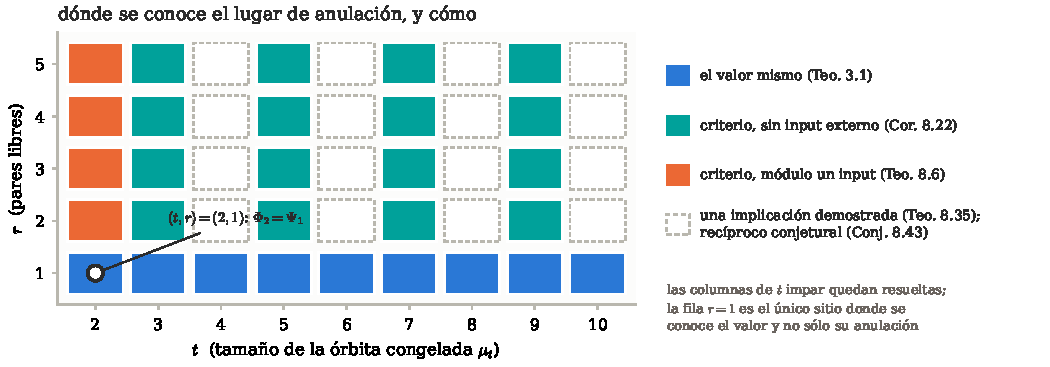
\includegraphics[width=\textwidth]{fig_plane_es.pdf}
\caption{La familia de dos parámetros, y lo que se sabe sobre ella. Cada celda es un alfabeto
$\zt\cup\{z_1^{\pm1},\dots,z_r^{\pm1}\}$; el color no se asigna a mano, sino que se calcula a partir
de los propios enunciados, con una regla por línea del artículo. La fila $r=1$ es el único sitio
donde se conoce el \emph{valor} y no sólo su anulación, que es el Teorema \ref{thm:main}; las
columnas de $t$ impar las resuelve el Corolario \ref{cor:oddgen} sin ningún input externo; la columna
$t=2$, el Teorema \ref{conj:crit}, que usa uno. En las celdas restantes el Teorema \ref{thm:suff}
prueba una implicación y la Conjetura \ref{conj:general} es la otra. La esquina marcada es donde se
encuentran las dos mitades del artículo: allí $\Phi_2=\Psi_1$, y es el único alfabeto que ven las
dos. Calculada por \texttt{anc/fig\_plane.py}.}
\label{fig:plane}
\end{figure} El Teorema \ref{thm:main}
es $r=1$: un par, todo $t$, y ahí tenemos el valor y no sólo su anulación.
El Teorema \ref{conj:crit} es $t=2$: cualquier número de pares, la órbita más pequeña. Y el Corolario
\ref{cor:oddgen} es \emph{todo $t$ impar y todo $r$} a la vez: allí el carácter se anula si y sólo si
falta una clase de residuos, de modo que la rama concéntrica es un fenómeno exclusivo de $t$ par. La
tercera de las tres no es un borde sino medio plano, y es además la más barata --- sale del argumento
extremal de la \S\ref{sec:extremal} sin ningún input externo, mientras que la segunda necesita el
Teorema \ref{thm:PvW}. Fuera de esas tres regiones el lugar no está resuelto, pero ya no está intacto. El
Teorema \ref{thm:suff} da una condición sobre el conjunto beta --- una reflexión de su parte de
exceso, y un incremento que da en el centro --- que fuerza la anulación del carácter para
\emph{todo} $t$ y todo $r$, mediante una involución que empareja todos los términos del desarrollo;
el Corolario \ref{cor:necgen} da una condición necesaria por el otro lado. Que las dos se encuentren
es la Conjetura \ref{conj:general}, y lo que las separa es una sola implicación, que la
\S\ref{sec:rigidity} muestra que no puede venir del estrato en el que ese argumento trabaja. El
fórmula de producto del Teorema \ref{thm:main} ya falla en $r=2$, por (D1) ---que no exista tal
fórmula para ningún $r\ge2$ es la Conjetura \ref{conj:rank2}, y no algo que demostremos---, así que
pasada la línea $r=1$ el lugar es lo que podemos ofrecer.

Hay algo que el alfabeto delata y que merece decirse aquí y no de pasada. Tiene una lectura en
teoría de representaciones ---de la clase que \cite{CK09} registran como ausente para sus
factorizaciones, y con ellos \cite{AB19} y \cite{AK25}--- y el mecanismo no es nuestro: el alfabeto
es cerrado por inversión, luego
un elemento del toro de $O(N)$ de determinante $(-1)^{t+1}$, de modo que para $t$ par vive en la
componente no identidad, donde un carácter es un carácter \emph{entrelazado} en el sentido de
Jantzen \cite{Jantzen} y Kumar--Lusztig--Prasad \cite{KLP} y el plegado lo da el álgebra de Lie de
órbitas. La Observación \ref{rem:twining} lo precisa y el Lema \ref{lem:AtoSp} lo concreta ---allí el
álgebra plegada es $C_r$ y el carácter entrelazado es un carácter simpléctico sin más. La
demostración del Teorema \ref{thm:main} no usa nada de eso, y por eso lo enunciamos como lectura y no
como método.

El artículo se organiza como sigue. Fijamos notación y recordamos las dos evaluaciones sobre las que
construimos en la Sección \ref{sec:background}. En la Sección \ref{sec:main} enunciamos el teorema
principal, identificamos sus tres enteros en términos del núcleo y del $t$-cociente, describimos las
particiones que no consiguen separar y registramos el criterio de
anulación y la imagen de la aplicación resultante. La Sección \ref{sec:proof} contiene la
demostración. En la Sección \ref{sec:independence} comparamos el teorema con el criterio de
independencia de \cite{AK25} y determinamos la familia adicional que adquiere en el lugar recíproco.
En la Sección \ref{sec:enum} leemos el teorema como una enumeración y ensamblamos, en $t=2$, la
involución que invierte el signo que esa enumeración pide, y en la Sección
\ref{sec:sharp} probamos cuatro deformaciones del alfabeto, cada una de las cuales destruye la
identidad. La Sección \ref{sec:zeros} determina
el lugar de anulación en $t=2$ para un número arbitrario de pares recíprocos ---y, sin ningún coste
externo, también en todo $t$ impar---, lee ese criterio sobre el grupo como una rigidez frente al
giro por el determinante, y da un criterio suficiente, con recíproco conjetural, para $t$ y $r$
arbitrarios. La Sección \ref{sec:verif} recoge las
comprobaciones numéricas y la Sección \ref{sec:open} los problemas abiertos.

%======================================================================
\section{Preliminares y notación}\label{sec:background}

Seguimos la notación de \cite{AK22,AK25}. Todos los grupos algebraicos son aquí sobre $\CC$; en
particular $O(N)$ significa $O(N,\CC)$, que es lo que da un alfabeto cerrado por $x\mapsto x^{-1}$
cuando se permite a sus letras salir de la circunferencia unidad.

\subsection{Particiones, conjuntos beta, núcleos y cocientes}
Una partición $\lambda=(\lambda_1,\dots,\lambda_n)$ es una sucesión débilmente decreciente de enteros
no negativos; $\PP_n$ denota el conjunto de particiones de longitud a lo sumo $n$, $|\lambda|$ el
tamaño y $\ell(\lambda)$ la longitud. En todo el texto $t\ge2$ es un entero fijo, $\zeta$ una raíz
$t$-ésima primitiva de la unidad, $\zt=\{1,\zeta,\dots,\zeta^{t-1}\}$, y
\[
N:=t+2 .
\]
Para $\lambda\in\PP_N$ el \emph{conjunto beta} es $\beta(\lambda)=(\beta_1,\dots,\beta_N)$ con
$\beta_j=\lambda_j+N-j$, de modo que $\beta_1>\beta_2>\dots>\beta_N\ge0$; indexamos por
\emph{columnas} $j=1,\dots,N$, y observamos que un $\beta$ mayor significa un índice de columna menor.
Para $0\le i\le t-1$ escribimos $n_i(\lambda)$ para el número de partes de $\beta(\lambda)$
congruentes con $i$ módulo $t$, de manera que
\begin{equation}\label{eq:excess}
\sum_{i=0}^{t-1}n_i(\lambda)=N=t+2 .
\end{equation}
Llamamos \emph{perfil de residuos} de $\lambda$ al vector
$\bigl(n_0(\lambda),\dots,n_{t-1}(\lambda)\bigr)$. Por \eqref{eq:excess},
$\sum_i\bigl(n_i(\lambda)-1\bigr)=2$: o alguna clase está vacía, o, estando todas ocupadas, el
exceso sobre una cada una es exactamente dos, y sólo hay dos particiones de dos. De modo que un
perfil es de exactamente uno de tres tipos: \emph{degenerado}, si algún $n_i=0$; \emph{de dos
clases}, si dos entradas valen $2$; o \emph{de tamaño tres}, si una entrada vale $3$. Todo lo que
sigue en este artículo está gobernado por cuál de los tres se da.
Sea $\sigma\in S_N$ la permutación que reordena las partes de $\beta(\lambda)$ agrupándolas por clase
de residuo, con las clases en orden creciente y los valores dentro de cada clase en orden
decreciente; es la permutación de \cite[(2.1)]{AK25}. Escribimos $\core_t(\lambda)$ y
$\quot_t(\lambda)=(\lambda^{(0)},\dots,\lambda^{(t-1)})$ para el $t$-núcleo y el $t$-cociente,
definidos a partir de $\beta(\lambda)$ como en \cite[\S2.1]{AK25}. Por \cite{GKS90}, los $t$-núcleos
están en biyección con los vectores del retículo de raíces de tipo $A_{t-1}$, y los recuentos de
residuos $n_i$ son las coordenadas naturales.

Ponemos $\zb:=z^{-1}$, $z=e^{\theta}$, y abreviamos
\[
f(u):=z^{u}-z^{-u}=2\sinh(u\theta),\qquad
V:=\prod_{0\le k<k'\le t-1}\bigl(\zeta^{k'}-\zeta^{k}\bigr).
\]
Para un conjunto $S$ de columnas, $b_S$ es la palabra de residuos $\beta_j\bmod t$ para $j\in S$
leída en orden creciente de columna, e $\inv(b_S)$ su número de inversiones. Usamos el bialternante
\[
s_\lambda(x_1,\dots,x_N)=\frac{\det\bigl(x_i^{\beta_j}\bigr)_{i,j=1}^N}
{\det\bigl(x_i^{N-j}\bigr)_{i,j=1}^N}.
\]

\subsection{Las dos evaluaciones sobre las que construimos}
Recordamos los dos enunciados entre los que se sitúa el presente resultado. El primero es la
evaluación de Littlewood, en la forma de \cite[Teorema 2.2]{AK25}.

\begin{theorem}[{\cite[Teorema IX]{LR34}}]\label{thm:LR}
Sea $\lambda\in\PP_t$. Entonces
\[
s_\lambda(1,\zeta,\dots,\zeta^{t-1})=
\begin{cases}
(-1)^{\binom{t}{2}}\sgn(\sigma) & \text{si }\core_t(\lambda)=\varnothing,\\
0 & \text{en otro caso.}
\end{cases}
\]
\end{theorem}

El segundo es el criterio de independencia que extendemos, \cite[Teorema 5.3]{AK25}; enunciamos el
caso que necesitamos. Sea $f_\lambda$ un carácter universal de tipo $s$, $sp$ u $o$, sea $Y$ un
conjunto de $m$ variables y sean $x_1,\dots,x_{n-tm}$ libres. Entonces
\begin{equation}\label{eq:AK53}
f_\lambda(x_1,\dots,x_{n-tm},Y,\zeta Y,\dots,\zeta^{t-1}Y)=f_\lambda(x_1,\dots,x_{n-tm})
\quad\Longleftrightarrow\quad \lambda=\core_t(\lambda),
\end{equation}
para $\lambda\in\PP_{n-tm}$. El criterio es uniforme en el tipo ---un solo enunciado para $s$, $sp$ y
$o$ a la vez---, que es lo que lo hace citable aquí: nuestro alfabeto es un alfabeto de $GL$, y lo
que le preguntamos es una cuestión sobre una especialización y no sobre un grupo. Tomando $m=1$,
$Y=(1)$ y $(x_1,x_2)=(z,\zb)$ se obtiene $n=t+2$ y nuestro alfabeto, pero esa sustitución es
justamente donde se abandona la hipótesis de que $x_1,x_2$ sean libres. Así que \eqref{eq:AK53} no se
está aplicando sobre el lugar recíproco; se le está preguntando por él, que es la
\S\ref{sec:independence}.

\begin{remark}\label{rem:notacase}
El enunciado más próximo de la literatura añade dos letras extra, igual que nosotros, de modo que
conviene registrar por qué no contiene \eqref{eq:object}. Kumari \cite[Teorema 2.2]{Kum24} evalúa
$s_\lambda(X,\zeta X,\dots,\zeta^{t-1}X,\,y,\zeta y,\dots,\zeta^{m-1}y)$; con $X=(1)$ y $m=2$ el
bloque añadido es $\{y,\zeta y\}$, mientras que el nuestro es $\{z,z^{-1}\}$. Los dos coinciden solo
cuando $z^{2}=\zeta^{\pm1}$, un conjunto finito de puntos y no una variable libre. Lo mismo vale para
la única variable libre extra de \cite[Teorema 2.7]{AK22} y para el Teorema XI de
Littlewood--Richardson.
\end{remark}

%======================================================================
La Figura \ref{fig:beta} hace todo el diccionario sobre una forma concreta.

\begin{figure}[!ht]
\centering
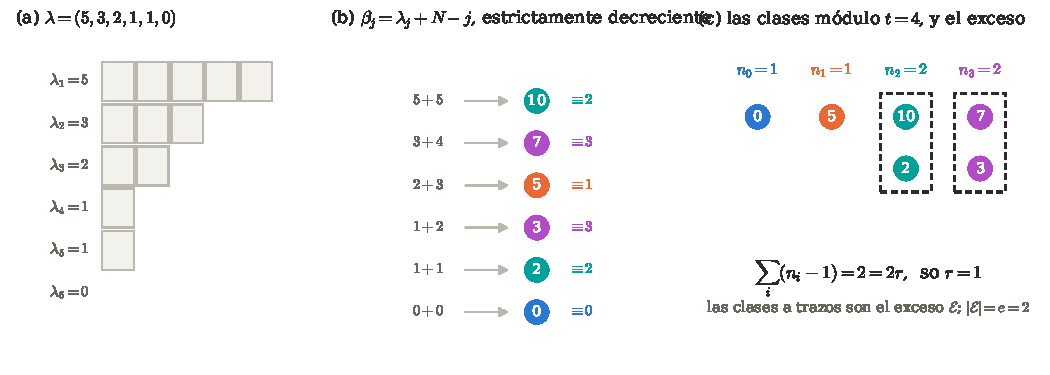
\includegraphics[width=\textwidth]{fig_beta_es.pdf}
\caption{El diccionario sobre el que corre el resto del artículo, con $\lambda=(5,3,2,1,1,0)$ y
$t=4$. \emph{(a)} la forma, rellenada hasta $N$ partes. \emph{(b)} $\beta_j=\lambda_j+N-j$, que
convierte una sucesión débilmente decreciente en una estrictamente decreciente y por tanto en un
conjunto; cada valor se colorea después según su residuo módulo $t$. \emph{(c)} el perfil de
residuos $(n_0,\dots,n_{t-1})$ y el recuento \eqref{eq:excess}: $\sum_i(n_i-1)=2r$ siempre, de modo
que cuando toda clase está ocupada las clases con $n_i\ge2$ ---el exceso $\mathcal{E}$, a trazos---
llevan exactamente $2r$ elementos más de uno cada una. Si alguna está vacía la suma sigue valiendo
$2r$ pero ya no es un exceso: ésa es la rama degenerada, que se resuelve la primera.
Todo lo que el artículo demuestra es un enunciado sobre ese dibujo.
Calculada por \texttt{anc/fig\_intro.py}.}
\label{fig:beta}
\end{figure}

\section{La evaluación}\label{sec:main}

\keybox{\emph{El teorema en una frase.} El valor depende de $\lambda$ a través de su perfil de
residuos, una terna de intervalos $(d_1,d_2,d_3)$ y un signo, y de nada más: una partición
arbitrariamente grande queda comprimida a tres enteros y un signo.}

\begin{theorem}\label{thm:main}
Sean $t\ge2$ y $\lambda\in\PP_N$, con $N=t+2$.
\begin{enumerate}
\item[\rm(i)] Si $n_i(\lambda)=0$ para algún $i$, entonces $\Phi_t(\lambda;z)=0$.
\item[\rm(ii)] En caso contrario, por \eqref{eq:excess}, o bien exactamente dos clases de residuos
tienen $n_i=2$, o bien exactamente una tiene $n_i=3$. Sean $r_A\le r_B$ los residuos implicados y
sean
\[
A=\{a_1>a_2\},\qquad B=\{b_1>b_2\}
\]
en el primer caso las partes de $\beta(\lambda)$ en las clases $r_A$ y $r_B$, y en el segundo los dos
pares solapados $A=\{p,q\}$, $B=\{q,r\}$ de la clase $\{p>q>r\}$, de modo que $r_A=r_B$. Pongamos
\[
d_1=a_1-a_2,\qquad d_2=b_1-b_2,\qquad
\tilde d_3=a_1+a_2-b_1-b_2,\qquad d_3=|\tilde d_3| ,
\]
y llamemos a $\tilde d_3$ el \emph{acoplamiento orientado}. Si $\tilde d_3=0$, entonces
$\Phi_t(\lambda;z)=0$. En caso contrario, con $z=e^\theta$,
\begin{equation}\label{eq:main}
\boxed{\;\;\Phi_t(\lambda;z)\;=\;\varepsilon_\lambda\cdot
\frac{\sinh(d_1\theta/2)\,\sinh(d_2\theta/2)\,\sinh(d_3\theta/2)}
{\sinh^2(t\theta/2)\,\sinh\theta}\;\;}
\end{equation}
donde, escribiendo $j_{A_1}$ y $j_{B_1}$ para las columnas que llevan $a_1$ y $b_1$, $S$ para el
complementario de $\{j_{A_1},j_{B_1}\}$ en $\{1,\dots,N\}$, y $b_S$ para la palabra de residuos de
$\beta(\lambda)$ sobre $S$ leída en orden creciente de columna,
\begin{equation}\label{eq:sign}
\varepsilon_\lambda\;=\;(-1)^{\,t+\binom{N+1}{2}}\;
(-1)^{\,j_{A_1}+j_{B_1}+\inv(b_S)}\;\sgn(a_1-b_1)\;\sgn(\tilde d_3).
\end{equation}
\end{enumerate}
Cada uno de los cuatro factores es $\pm1$ ---el último porque $\tilde d_3\ne0$ es exactamente la
hipótesis de {\rm(ii)}---, luego $\varepsilon_\lambda=\pm1$. En el perfil de tamaño tres $r_A=r_B$ y
$\tilde d_3=p-r>0$, luego ese factor es $+1$.

El lado izquierdo es un polinomio de Laurent en $z$. Leemos \eqref{eq:main} como identidad en
$\CC(z)$; tras la cancelación el lado derecho es también un polinomio de Laurent, y en los ceros del
denominador ---$z=\pm1$ y $z^t=1$--- usamos esa continuación. Así lo hacemos en \S\ref{sec:enum},
donde el valor se toma en $z=1$.
\end{theorem}

\noindent Separar $d_3$ en su tamaño y su orientación no es contabilidad. El signo \eqref{eq:sign}
necesita la orientación y la fórmula necesita solo el tamaño, y en $\tilde d_3=0$ la orientación no
existe: un enunciado que lleve $\sgn(a_1+a_2-b_1-b_2)$ y afirme que vale $\pm1$ es falso sobre el
lugar concéntrico, donde ese argumento es cero. El valor allí es $0$ por el factor
$\sinh(d_3\theta/2)$, de modo que nada de lo que viene después cambia; lo que cambia es que el caso
queda ahora excluido antes de escribir el signo, y no después.

Escribimos
\[
d(\lambda):=(d_1,d_2,d_3)
\]
y lo llamamos la \emph{terna de intervalos} de $\lambda$, siguiendo la lectura
\eqref{eq:intervals}; y llamamos a $d_3$ el \emph{término de acoplamiento}, por ser el único de los
tres que mezcla las dos clases distinguidas.

Conviene dar nombre al dato completo, porque el teorema se lee mejor como un enunciado sobre él que
como una fórmula. Pongamos
\begin{equation}\label{eq:invariant}
\boxed{\;\;I_t(\lambda)\;:=\;\begin{cases}
0 & \text{si el perfil de residuos es degenerado, o }\tilde d_3=0,\\[2pt]
\bigl(d_1,d_2,d_3,\varepsilon_\lambda\bigr) & \text{en otro caso},
\end{cases}\;\;}
\end{equation}
y llamémoslo el \emph{invariante de la evaluación} de $\lambda$. Su primera rama es exactamente el
lugar de anulación del Corolario \ref{cor:zero}, y es una rama y no dos porque en todo él no hay
signo que registrar: \eqref{eq:sign} necesita $\tilde d_3\ne0$. El Teorema \ref{thm:main} dice
entonces dos cosas a la vez. Primera, que $\Phi_t$ \emph{factoriza a través} de $I_t$: la aplicación
$\lambda\mapsto\Phi_t(\lambda;z)$ es la composición de $\lambda\mapsto I_t(\lambda)$ con una función
del invariante solo. Segunda, que ese invariante es \emph{completo} para esta evaluación: si dos
particiones tienen el mismo $I_t$ tienen el mismo $\Phi_t$, sean del tamaño que sean. La completitud
es lo que hace que la compresión anunciada más arriba merezca un nombre y no solo una observación
---dice que el invariante no es un resumen cómodo de la dependencia, sino la dependencia entera--- y
convierte la pregunta natural siguiente, qué olvida el invariante, en una pregunta bien planteada.
La Proposición \ref{prop:minimal} cierra la pregunta por el otro lado: una vez leída la terna como
multiconjunto, tampoco puede suprimirse nada de $I_t$. Así que la \S\ref{sec:fibrelattice} resuelve
qué se olvida para la terna y el Problema \ref{prob:fibres} es lo que deja
el signo. Los $(d_1,d_2,d_3)$ de la Figura \ref{fig:image} son
los valores que toma este invariante, dibujados.

Esa factorización es una sola tubería, y cada flecha pierde información que ya no vuelve:
% multline y no \[...\]: la cadena entera no cabe en una caja de 436 pt, y una formula sin puntos
% de corte no se parte sola.  El corte va tras el paso que pierde los intervalos, que es donde el
% lector para de todos modos.
\begin{multline*}
\lambda\;\longrightarrow\;\beta(\lambda)\;\longrightarrow\;
\bigl(\text{perfil de residuos},\ \text{los dos intervalos distinguidos}\bigr)\\
\longrightarrow\;\bigl(d_1,d_2,d_3,\varepsilon_\lambda\bigr)\;\longrightarrow\;\Phi_t(\lambda;z).
\end{multline*}
Los intervalos hay que llevarlos junto al perfil: el perfil dice qué clases son las distinguidas y
nada sobre dónde caen sus números beta, de modo que no determina la terna.
Coordenada a coordenada, el invariante reparte el trabajo así.

\begin{center}\small
\begin{tabular}{ll}
\toprule
dato de $\lambda$ & qué controla\\
\midrule
perfil de residuos & la rama degenerada de anulación\\
las dos longitudes $d_1,d_2$ & los dos primeros factores\\
la distancia entre los centros, $d_3$ & el factor de acoplamiento, y la rama concéntrica de anulación\\
la orientación $\sgn(\tilde d_3)$ & un factor del signo\\
el signo de ordenación $\varepsilon_\lambda$ & el signo global\\
\bottomrule
\end{tabular}
\end{center}

\noindent Ninguna de las dos ramas de anulación es la otra: el perfil no puede ver la concéntrica, y
la terna no puede ver la degenerada, y por eso el criterio del Corolario \ref{cor:zero} tiene dos
cláusulas y la \S\ref{sec:main} dedica una proposición a decir dónde vive cada una.

\keybox{Un solo recuento recorre el artículo. Con $t$ clases de residuos, $N=t+2$ partes y toda
clase ocupada, el exceso es exactamente dos, de modo que por \eqref{eq:excess} un perfil sólo
puede ser degenerado, de dos
clases o de tamaño tres: esa tricotomía es la forma del Teorema \ref{thm:main}, la
división en casos de su demostración en la \S\ref{sec:proof}, y la primera rama del lugar de
anulación en la \S\ref{sec:zeros}. Dos clases distinguidas son lo que el par recíproco tiene que
acoplar, y de ahí exactamente un término de acoplamiento y tres factores en vez de dos.}

El recuento de tres tiene una segunda explicación, que no debe nada a la demostración. El exceso
dos da dos clases distinguidas, que son dos intervalos sobre la recta beta, y un par de intervalos
son cuatro números $(a_1,a_2,b_1,b_2)$. Los tres argumentos de \eqref{eq:main} ven qué forma tiene
ese par y no dónde está: un desplazamiento común $\beta\mapsto\beta+m$ deja $d_1$, $d_2$ y
$\tilde d_3$ intactos. Así que lo único que puede entrar en ellos es un funcional lineal que mate la
traslación común, y esos forman el hiperplano $\sum\alpha_i=0$ del dual de dimensión cuatro: un
espacio de dimensión exactamente \emph{tres}. La terna $d_1=(1,-1,0,0)$, $d_2=(0,0,1,-1)$ y
$\tilde d_3=(1,1,-1,-1)$ es una base de él. Módulo la traslación común, un par de intervalos tiene
tres coordenadas lineales independientes, y de ahí sale el recuento de tres. Lo que el Teorema
\ref{thm:main} añade, y que el recuento de dimensiones \emph{no} fuerza, es que en esta
especialización esas tres coordenadas \emph{se separan multiplicativamente}: un producto con un
factor de cada una, y no otra función de tres variables.

El \emph{valor} no es invariante por traslación, y merece la pena decirlo, porque lo que es en su
lugar es una restricción sobre el signo. Un desplazamiento $\beta\mapsto\beta+m$ es
$\lambda\mapsto\lambda+(m^N)$, y $s_{\lambda+(m^N)}(A)=\det(A)^{m}s_\lambda(A)$ para cualquier
alfabeto $A$, así que por \eqref{eq:object}
\begin{equation}\label{eq:shift}
\Phi_t\bigl(\lambda+(m^N);z\bigr)\;=\;(-1)^{(t+1)m}\,\Phi_t(\lambda;z).
\end{equation}
Para $t$ impar el valor es invariante; para $t$ par un desplazamiento impar lo invierte. La terna no
se mueve, de modo que toda esa inversión la lleva $\varepsilon_\lambda$ --- lo que convierte a
\eqref{eq:shift} en una comprobación de \eqref{eq:sign} que no cuesta nada y que el signo supera,
sobre las formas de la \S\ref{sec:verif}. Es además la razón de que el lema haya que enunciarlo sobre
la terna y no sobre el valor: para $t$ par el valor no es función de la clase de traslación de la
terna.

El signo \eqref{eq:sign} es un signo de ordenación, de la misma especie que el del Teorema
\ref{thm:LR}; la Proposición \ref{rem:sign} registra más abajo una expresión más corta para él, en la
notación de \cite{AK25}.

El miembro derecho de \eqref{eq:main} es un cociente, y el contenido del teorema es que ese cociente
es un polinomio de Laurent en $z$. Para $t$ impar el factor $\sinh(t\theta/2)$ por separado no es un
monomio de Laurent, de modo que los tres factores no están individualmente en $\ZZ[z,z^{-1}]$; solo
lo está su combinación. Aun así el enunciado es uniforme en $t$.

\begin{corollary}\label{cor:zero}
$\Phi_t(\lambda;z)\equiv0$ si y solo si alguna clase de residuos módulo $t$ es vacía, o
$a_1+a_2=b_1+b_2$. En particular el perfil de tamaño tres nunca se anula.
\end{corollary}

\noindent La anulación es idéntica en $z$, no en un punto: cuando ocurre, $\lambda$ no aporta nada en
ningún elemento de la familia de un parámetro que barre el par recíproco. Ésa es la forma en que se
planteaba la pregunta de Prasad en la \S\ref{sec:background}, y el sentido en que \eqref{eq:object}
se lee fuera de la combinatoria ---siendo la mitad congelada del alfabeto una holonomía de orden
finito, y el par libre lo que queda del toro---.

\begin{corollary}\label{cor:chars}
Escribamos $\chi_k(z)=(z^{k+1}-z^{-k-1})/(z-z^{-1})$ para el carácter del $\mathfrak{sl}_2$-módulo
irreducible de dimensión $k+1$ cuando $k\ge0$ es entero. Para $k$ semientero conservamos la misma
fórmula, leída en $u=z^{1/2}$; es entonces notación y no un carácter, porque los factores por
separado no son de Laurent en $z$. Entonces
\eqref{eq:main} puede escribirse sin ninguna exponencial y sin convenio alguno para $\theta$:
\begin{equation}\label{eq:chiratio}
\boxed{\;\;\Phi_t(\lambda;z)\;=\;\varepsilon_\lambda\,
\frac{\chi_{\frac{d_1}{2}-1}(z)\;\chi_{\frac{d_2}{2}-1}(z)\;\chi_{\frac{d_3}{2}-1}(z)}
{\chi_{\frac{t}{2}-1}(z)^{2}}\;\;}
\end{equation}
Para $t=2$ el denominador es $\chi_0=1$ y todo $d_i$ es par, luego $\Phi_2$ es sin más un producto
con signo de tres caracteres $\mathfrak{sl}_2$. Para $t$ impar los índices son semienteros, que es el
enunciado de arriba en otra forma: los tres factores no son Laurent por separado, y solo lo es el
cociente. Cada factor se lee en $u=z^{1/2}$ y cambia de signo bajo $u\mapsto-u$ exactamente cuando
su índice es semientero; como $d_1+d_2+d_3$ es par ---tiene la paridad de
$d_1+d_2+\tilde d_3=2(a_1-b_2)$---, el cociente no cambia, y es el polinomio de Laurent en $z$ de
\eqref{eq:main}.
\end{corollary}

\begin{proof}
Escribamos $f(u)=z^{u}-z^{-u}=2\sinh(u\theta)$, de modo que $\chi_k=f(k+1)/f(1)$. El numerador de
\eqref{eq:main} es $f(d_1/2)f(d_2/2)f(d_3/2)/8$ y su denominador es $f(t/2)^2f(1)/8$, así que
\eqref{eq:main} vale $\varepsilon_\lambda f(d_1/2)f(d_2/2)f(d_3/2)/\bigl(f(t/2)^2f(1)\bigr)$;
sacando tres factores $f(1)$ del numerador y dos del denominador se obtiene \eqref{eq:chiratio}.
\end{proof}

\subsection{Los tres enteros vienen del cociente}
Lo siguiente identifica $(d_1,d_2,d_3)$ en el idioma de la línea de raíces de la unidad. Para una
partición $\nu$ ponemos $k(\nu)=\nu_1-\nu_2$, su contenido $\mathfrak{sl}_2$.

\begin{proposition}\label{prop:quotient}
En el perfil de dos clases, con $\quot_t(\lambda)=(\lambda^{(0)},\dots,\lambda^{(t-1)})$,
\[
d_1=t\bigl(k(\lambda^{(r_A)})+1\bigr),\qquad
d_2=t\bigl(k(\lambda^{(r_B)})+1\bigr),\qquad
\tilde d_3=t\bigl(|\lambda^{(r_A)}|-|\lambda^{(r_B)}|\bigr)+2(r_A-r_B) .
\]
En el perfil de tamaño tres la única componente distinguida $\lambda^{(r_A)}$ tiene tres partes y
\[
d_1=t\bigl(\lambda^{(r_A)}_1-\lambda^{(r_A)}_2+1\bigr),\quad
d_2=t\bigl(\lambda^{(r_A)}_2-\lambda^{(r_A)}_3+1\bigr),\quad \tilde d_3=d_1+d_2 .
\]
\end{proposition}

\begin{proof}
Escribamos $a_i=t\tilde a_i+r_A$. La clase $r_A$ lleva dos números beta, luego
$\lambda^{(r_A)}=(\tilde a_1-1,\tilde a_2)$ por la definición del cociente, de donde
$k(\lambda^{(r_A)})=\tilde a_1-\tilde a_2-1$ y $d_1=t(\tilde a_1-\tilde a_2)$, que es la primera
identidad; la segunda es el mismo cálculo. Para la tercera, $\tilde a_1+\tilde a_2=|\lambda^{(r_A)}|+1$
y análogamente para $B$, luego $a_1+a_2-b_1-b_2=t(|\lambda^{(r_A)}|-|\lambda^{(r_B)}|)+2(r_A-r_B)$. El
caso de tamaño tres es idéntico con $\lambda^{(r_A)}=(\tilde p-2,\tilde q-1,\tilde r)$.
\end{proof}

Para $t=2$ la tercera identidad se lee $\tilde d_3=2\bigl(|\lambda^{(0)}|-|\lambda^{(1)}|-1\bigr)$, lo que
ya muestra que $\tilde d_3$ es un funcional sobre los tamaños del cociente y no sobre el vector de
residuos, luego tampoco sobre el retículo de raíces de tipo $A_{t-1}$ bajo la correspondencia de
Garvan--Kim--Stanton \cite{GKS90} entre ese retículo y los $t$-núcleos. La condición $r_B-r_A=t/2$,
que gobierna la familia del Teorema \ref{thm:extra}, es un elemento de orden dos del cociente
correspondiente, y esa es la fuente de los fenómenos de paridad de todo el artículo.

\begin{proposition}[el lugar concéntrico]\label{rem:lattice}
En el perfil de dos clases, ordenado de modo que $r_A<r_B$,
\[
\boxed{\;\;d_3=0\quad\Longleftrightarrow\quad t\ \text{es par},\quad r_B-r_A=\tfrac t2,
\quad\text{y}\quad \bigl|\lambda^{(r_A)}\bigr|=\bigl|\lambda^{(r_B)}\bigr|+1\;\;}
\]
En particular, para $t$ impar $\Phi_t(\lambda;z)=0$ si y solo si alguna clase de residuos módulo $t$
es vacía: allí la cláusula concéntrica del Corolario \ref{cor:zero} es vacua.
\end{proposition}

\begin{proof}
Como $a_1,a_2\equiv r_A$ y $b_1,b_2\equiv r_B$ módulo $t$, la igualdad $a_1+a_2=b_1+b_2$ fuerza
$2r_A\equiv2r_B$, es decir $t\mid2(r_B-r_A)$. Para $t$ impar esto da $t\mid r_B-r_A$ y por tanto
$r_A=r_B$, que es el perfil de tamaño tres, donde $d_3=d_1+d_2>0$ por la Proposición
\ref{prop:quotient}. Para $t$ par y $0\le r_A<r_B\le t-1$ la única solución de $t\mid2(r_B-r_A)$ es
$r_B-r_A=t/2$. Escribiendo $a_1+a_2=t\bigl(|\lambda^{(r_A)}|+1\bigr)+2r_A$ como en la demostración
de la Proposición \ref{prop:quotient}, y análogamente para $B$, la igualdad se convierte en
$t\bigl(|\lambda^{(r_A)}|-|\lambda^{(r_B)}|\bigr)=2(r_B-r_A)=t$.
\end{proof}

Las dos cláusulas del Corolario \ref{cor:zero} viven, pues, en mitades distintas de la
descomposición núcleo--cociente, y esa es la respuesta a la pregunta que el criterio plantea. La
primera es una condición sobre el perfil de residuos, y por tanto sobre el $t$-núcleo: los
hiperplanos coordenados $n_i=0$ recortados sobre la rebanada $\sum_i n_i=t+2$, que no es el arreglo
de Coxeter de tipo $A_{t-1}$. La segunda no es una condición sobre el núcleo en absoluto; es un
único hiperplano en los tamaños del cociente, y los pares de residuos admisibles están indexados por
el elemento de orden dos $r_B-r_A=t/2$ y no por reflexión alguna. No puede existir ninguna
reformulación del criterio de anulación en términos de $\core_t(\lambda)$ solo, que es para $\Phi_t$
lo que la Observación \ref{rem:core} registra para $\Psi_r$.

\subsection{Lo que la terna olvida}\label{sec:fibrelattice}
La Proposición \ref{prop:quotient} lee la terna del cociente. Recorrida al revés, esa misma
lectura dice qué particiones no puede distinguir la terna, y lo dice exactamente. Nada de esto es
profundo ---es la biyección núcleo--cociente a perfil fijo--- pero es lo que convierte la
compresión del Teorema \ref{thm:main} de una imagen en un recuento.

\begin{proposition}[el estrato de dos clases es un retículo]\label{prop:fibrelattice}
Sean $t\ge2$, $N=t+2$, y sea $\mathcal{T}_t\subset\PP_N$ el conjunto de particiones de perfil de dos
clases. Enviar $\lambda$ a sus dos residuos distinguidos junto con su $t$-cociente es una biyección
\begin{equation}\label{eq:fibrelattice}
\mathcal{T}_t\;\xrightarrow{\ \sim\ }\!\!\!\coprod_{0\le r_A<r_B\le t-1}\!\!\!
\PP_2\times\PP_2\times\ZZ_{\ge0}^{\,t-2},
\qquad
\lambda\longmapsto\bigl(r_A,r_B;\ \lambda^{(r_A)},\lambda^{(r_B)};\ (m_i)_{i\ne r_A,r_B}\bigr),
\end{equation}
donde $m_i$ es la única parte de $\lambda^{(i)}$. Bajo ella $\core_t(\lambda)$ depende solo del par
$(r_A,r_B)$; escribimos $\kappa(r_A,r_B)$ para su tamaño. Entonces
\begin{equation}\label{eq:sizelattice}
|\lambda|\;=\;\bigl|\core_t(\lambda)\bigr|
+t\Bigl(\bigl|\lambda^{(r_A)}\bigr|+\bigl|\lambda^{(r_B)}\bigr|+\textstyle\sum_i m_i\Bigr).
\end{equation}
\end{proposition}

\begin{proof}
Una clase que lleva $n_i$ números beta $a_1>\dots>a_{n_i}$, escritos $a_j=t\tilde a_j+i$, aporta
$\lambda^{(i)}=(\tilde a_1-n_i+1,\dots,\tilde a_{n_i})$, de modo que una clase de tamaño $n_i$ da
una partición con a lo sumo $n_i$ partes, y toda partición así proviene de una única
$(\tilde a_j)$ estrictamente decreciente. En el perfil de dos clases los tamaños son $2,2$ y $1$
repetido $t-2$ veces, que es \eqref{eq:fibrelattice}; los residuos se registran en vez de olvidarse
porque el perfil forma parte del dato, y determinan $\core_t(\lambda)$ por la coordenada de
Garvan--Kim--Stanton de la Observación \ref{rem:core}. Entonces \eqref{eq:sizelattice} es la
biyección núcleo--cociente.
\end{proof}

\begin{corollary}[la fibra de la terna, y su función generatriz]\label{cor:fibregf}
Sea $(d_1,d_2,d_3)$ una terna de intervalos alcanzada en el perfil de dos clases, y pongamos
$k_A=d_1/t-1$ y $k_B=d_2/t-1$. Su fibra en $\mathcal{T}_t$ es infinita. Es la unión disjunta de las
ramas indexadas por los pares $r_A<r_B$ y los signos $\eta=\pm1$ para los que
\begin{equation}\label{eq:branch}
c:=\tfrac12\Bigl(\tfrac{\eta\,d_3-2(r_A-r_B)}{t}-k_A+k_B\Bigr)\ \in\ \ZZ ,
\end{equation}
dando los dos signos una única y misma rama cuando $d_3=0$. Sobre una rama los parámetros
libres son un entero $v\ge\max(0,c)$ y $(m_i)\in\ZZ_{\ge0}^{t-2}$, con
$\lambda^{(r_A)}=(v+k_A,v)$ y $\lambda^{(r_B)}=(v-c+k_B,v-c)$. En consecuencia
\begin{equation}\label{eq:fibregf}
\sum_{\lambda\ \mathrm{en\ la\ fibra}}\!\!q^{|\lambda|}
\;=\;\frac{\sum_{\mathrm{ramas}}q^{\,e}}{\bigl(1-q^{4t}\bigr)\bigl(1-q^{t}\bigr)^{t-2}},
\qquad e=\kappa(r_A,r_B)+t\bigl(k_A+k_B-2c\bigr)+4t\max(0,c),
\end{equation}
y el número de $\lambda$ en la fibra con $|\lambda|\le n$ es a la larga un cuasi-polinomio en $n$ de
grado $t-1$ ---a la larga, porque los desplazamientos $q^{\,e}$ del numerador dejan el recuento en
$0$ por debajo del menor de ellos---.
\end{corollary}

\begin{proof}
Por la Proposición \ref{prop:quotient} las dos primeras entradas fijan $k(\lambda^{(r_A)})$ y
$k(\lambda^{(r_B)})$, así que cada componente distinguida queda determinada por su tamaño solo;
escribiéndolas $(v+k_A,v)$ y $(u+k_B,u)$, la tercera entrada dice
$t\bigl((2v+k_A)-(2u+k_B)\bigr)+2(r_A-r_B)=\eta\,d_3$, que es \eqref{eq:branch} con $c=v-u$; el
valor absoluto de $d_3$ es lo que pone ahí los dos signos, y es vacuo en $d_3=0$.
Sustituyendo en \eqref{eq:sizelattice} queda $|\lambda|=e+4t\bigl(v-\max(0,c)\bigr)+t\sum_i m_i$, y
sumar las series geométricas en $v$ y en cada $m_i$ da \eqref{eq:fibregf}. Su denominador tiene
$t-1$ factores, de donde el grado.
\end{proof}

\begin{remark}[el signo no va de pasajero]\label{rem:signsees}
Dos lecturas, y la segunda es una advertencia. Primera: una fibra es infinita para todo $t$ y toda
terna alcanzada, que es lo que muestra la Figura \ref{fig:fibres} y lo que explica
\eqref{eq:fibregf} ---las columnas de ahí no se adelgazan porque una fibra es una sección de
retículo y no un accidente finito. Segunda: \eqref{eq:fibregf} es la fibra de la \emph{terna} y no
la de $I_t$. Las $t-2$ partes $m_i$ son invisibles para $(d_1,d_2,d_3)$ por la Proposición
\ref{prop:quotient}, y sería natural leerlas como direcciones a lo largo de las cuales $\Phi_t$ es
constante. No lo son, desde $t=3$: el signo sí las ve, como \eqref{eq:sign} permite, ya que
$\varepsilon_\lambda$ lleva $\inv(b_S)$, un estadístico de la palabra beta entera, mientras
\eqref{eq:fibrelattice} parte esa palabra en dos clases distinguidas y $t-2$ letras libres. Sobre
los rangos de la \S\ref{sec:verif} el signo es constante en $(m_i)$ a $v$ fijo en los $107$ huecos
de $t=2$, pero solo en $43$ de $62$ en $t=3$ y $26$ de $36$ en $t=4$. Qué hace el signo sobre una
rama es el Problema \ref{prob:fibres}.
\end{remark}

\subsection{La lectura por intervalos}\label{sec:intervals}
La Figura \ref{fig:intervals} dibuja \eqref{eq:intervals} en un ejemplo. El Corolario \ref{cor:zero}
se lee: el carácter se anula cuando una clase de residuos es vacía, o cuando los dos intervalos son
\emph{concéntricos}; y dos intervalos que comparten un extremo son concéntricos solo si coinciden,
por lo que el perfil de tamaño tres nunca se anula.

\begin{figure}[t]
\centering
\begin{tikzpicture}[font=\small,x=1.3cm,y=1.0cm]
\draw[blue!55!black,very thick] (1,1.25) -- (7,1.25);
\draw[blue!55!black,thick] (1,1.10) -- (1,1.40);
\draw[blue!55!black,thick] (7,1.10) -- (7,1.40);
\filldraw[blue!55!black] (4,1.25) circle (1.8pt);
\node[blue!55!black,above=9pt] at (4,1.25) {$A=\{7,1\}$,\quad $d_1=6$};
\draw[red!60!black,very thick] (2,-1.25) -- (5,-1.25);
\draw[red!60!black,thick] (2,-1.40) -- (2,-1.10);
\draw[red!60!black,thick] (5,-1.40) -- (5,-1.10);
\filldraw[red!60!black] (3.5,-1.25) circle (1.8pt);
\node[red!60!black,below=9pt] at (3.5,-1.25) {$B=\{5,2\}$,\quad $d_2=3$};
\draw[->,gray!70] (-0.55,0) -- (8.1,0) node[right,black]{$\beta$};
\foreach \b in {0,...,7} \draw[gray!45] (\b,-0.07) -- (\b,0.07);
\foreach \b in {3,6} \node[gray,font=\scriptsize,below=4pt] at (\b,0) {$\b$};
\foreach \b/\c/\r in {7/blue!55!black/1, 5/red!60!black/2, 2/red!60!black/2,
                      1/blue!55!black/1, 0/gray!55/0}
  {\filldraw[\c] (\b,0) circle (2.7pt);
   \node[\c,font=\scriptsize,below=4pt] at (\b,0) {$\b$};
   \node[\c,font=\scriptsize,above=4pt] at (\b,0) {$\r$};}
\draw[gray!70,dashed] (4,1.25) -- (4,-0.62);
\draw[gray!70,dashed] (3.5,-1.25) -- (3.5,-0.62);
\draw[{Latex[length=1.5mm]}-{Latex[length=1.5mm]},thick] (3.5,-0.62) -- (4,-0.62);
\node[font=\scriptsize,gray!60!black,anchor=west] at (-0.55,1.25) {residuo $1$};
\node[font=\scriptsize,gray!60!black,anchor=west] at (-0.55,-1.25) {residuo $2$};
\end{tikzpicture}
\caption{El mecanismo para $t=3$, $\lambda=(3,2)$: aquí $N=5$, $\beta=(7,5,2,1,0)$ con residuos
$(1,2,2,1,0)$ módulo $3$, de modo que ninguna clase es vacía y dos clases tienen tamaño dos. Los tres
argumentos de \eqref{eq:main} son las dos longitudes de los intervalos y el doble de la distancia
entre sus centros; la flecha doble corta marca esa distancia, aquí $\tfrac12$, de modo que $d_3=1$.}
\label{fig:intervals}
\end{figure}

\begin{example}
Para $t=3$, $\lambda=(3,2)$ como en la Figura \ref{fig:intervals}, $(d_1,d_2,d_3)=(6,3,1)$ y
\[
\Phi_3\bigl((3,2);z\bigr)=\varepsilon\,
\frac{\sinh(3\theta)\sinh(\theta/2)}{\sinh(3\theta/2)\sinh\theta}.
\]
Para $t=3$, $\lambda=(3,1)$ el perfil es el de tamaño tres, $(d_1,d_2,d_3)=(3,3,6)$ y
$\Phi_3=\varepsilon\,\chi_2(z)$. Para $t=4$, $\lambda=(1,1,1)$ se tiene $\beta=(6,5,4,2,1,0)$, la
clase $3$ es vacía y $\Phi_4=0$.
\end{example}

\subsection{La imagen de la aplicación}
El Teorema \ref{thm:main} envía toda partición con a lo sumo $N$ filas a tres enteros, de modo que
toda la familia colapsa sobre un subconjunto disperso de $\ZZ^3$. Por la Proposición
\ref{prop:quotient} las dos primeras coordenadas son múltiplos de $t$; la tercera no lo es, salvo en
el perfil de tamaño tres, donde $d_3=d_1+d_2$. La Figura \ref{fig:image} muestra la imagen para $t=3$
y $t=4$, coloreada por el número de particiones que colapsan en cada punto.

\begin{figure}[t]
\centering
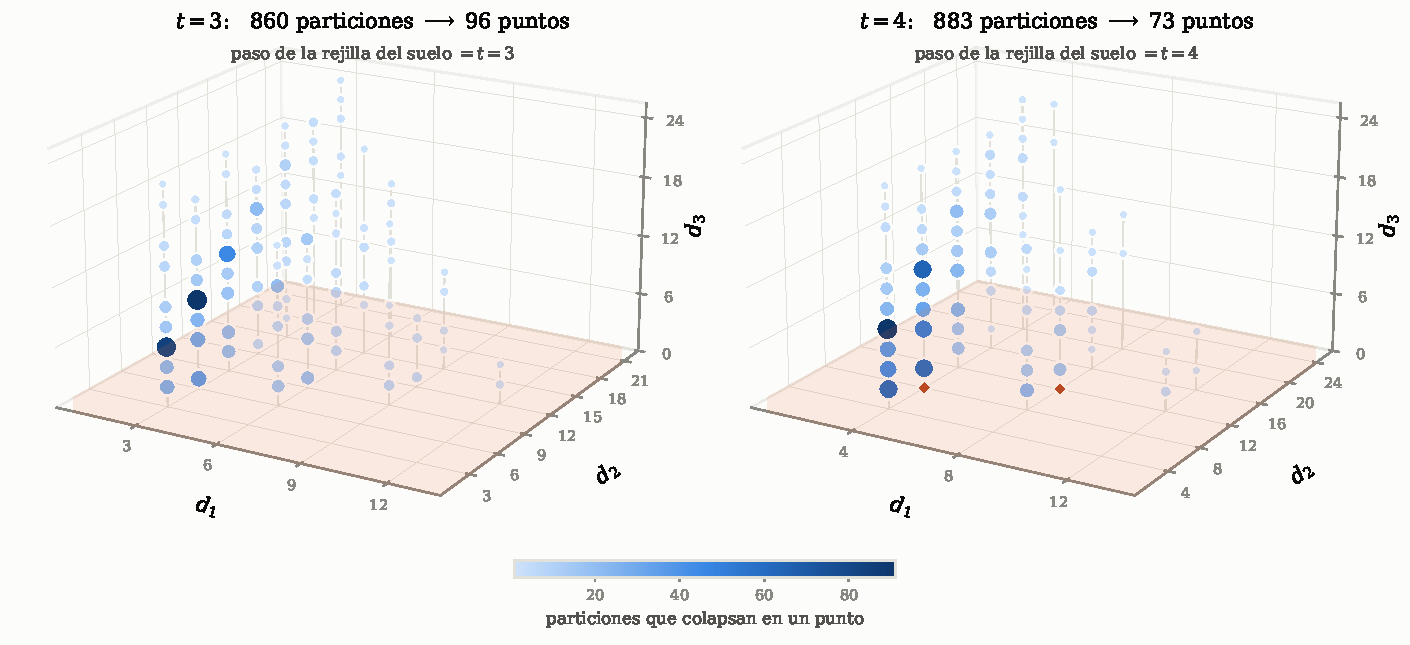
\includegraphics[width=\textwidth]{fig_image_es.pdf}
\caption{La imagen de $\lambda\mapsto(d_1,d_2,d_3)$ sobre todas las $\lambda$ con $|\lambda|\le20$ y
a lo sumo $t+2$ filas, para $t=3$ (izquierda) y $t=4$ (derecha), tomada \emph{salvo el intercambio de
$d_1$ y $d_2$}, bajo el cual \eqref{eq:main} es simétrica; sin esa identificación, y con $A$ y $B$ en
el orden $r_A\le r_B$ del Teorema \ref{thm:main}, los dos paneles llevan $126$ y $92$ puntos en vez
de $96$ y $73$. La compresión es el asunto de la figura: $860$
particiones aterrizan sobre $96$ ternas a la izquierda y $883$ sobre $73$ a la derecha, y el color y
el área dan el número de particiones que va a parar a cada una. El paso de la rejilla del suelo es $t$, pues
$d_1,d_2\in t\ZZ$ por la Proposición \ref{prop:quotient}; el plano sombreado $d_3=0$ es el lugar
concéntrico del Corolario \ref{cor:zero}, donde $s_\lambda$ se anula, así que esas formas no están
en la imagen y se dibujan sobre el plano como rombos. Los dos paneles son las dos paridades, que es
el contenido de la Proposición \ref{rem:lattice}: el impar no lleva ningún rombo, y no puede
llevarlo; el par lleva dos, que son entre ambos la imagen de $32$ particiones.}
\label{fig:image}
\end{figure}

La Figura \ref{fig:image} es una mitad de la imagen: muestra qué ternas se dan, no qué esconde una
terna. La Figura \ref{fig:fibres} es la otra mitad. Sobre cada celda del suelo $(d_1,d_2)$ se levanta
la columna de los tamaños $|\lambda|$ que aterrizan ahí, de modo que una columna es un conjunto de
particiones de tamaños distintos sobre las que $\Phi_t$ toma un único y mismo valor ---y las columnas
no se adelgazan al crecer $|\lambda|$, porque los valores están confinados a un retículo y las
particiones no. La más visible es la fibra de la partición vacía: en $t=3$ el invariante
$I_3=(3,3,2,+1)$ lo comparten $26$ particiones, de $19$ tamaños distintos entre $0$ y $20$, así que
$\Phi_3$ no distingue $\varnothing$ de una forma de veinte cajas.

\begin{figure}[!ht]
\centering
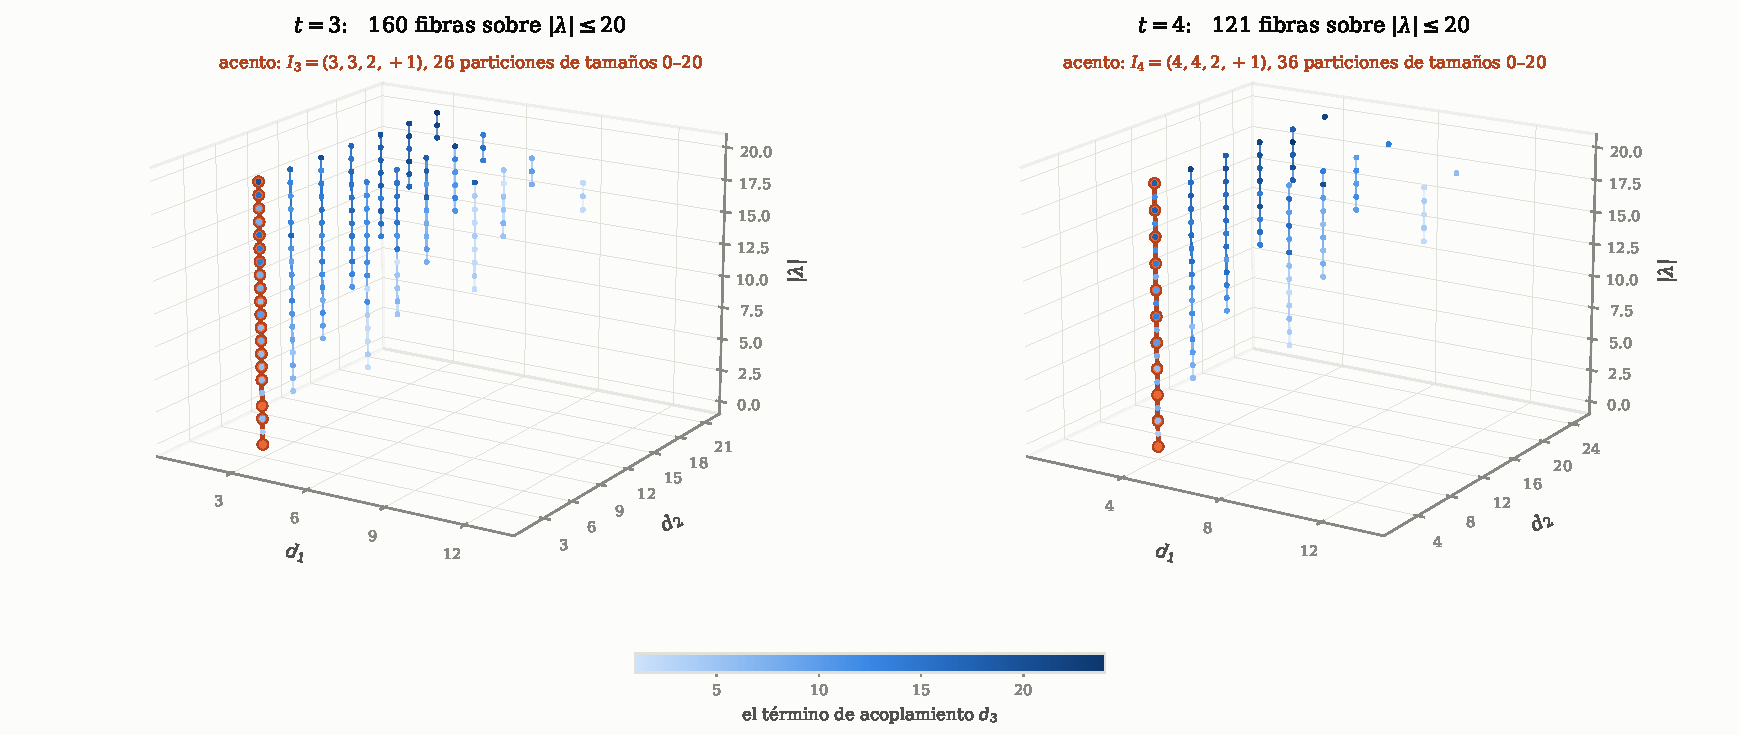
\includegraphics[width=\textwidth]{fig_fibres_es.pdf}
\caption{Las fibras del invariante de la evaluación \eqref{eq:invariant}, complemento de la Figura
\ref{fig:image}: el mismo rango $|\lambda|\le20$, con el término de acoplamiento pasado al color y el
tamaño $|\lambda|$ en el eje vertical. Una columna es una fibra, así que su altura es el rango de
tamaños que este alfabeto no sabe separar; las marcas del suelo son el retículo $t\ZZ$ de la
Proposición \ref{prop:quotient}, y solo está ocupada la mitad $d_1\le d_2$ porque la terna se toma
salvo el intercambio, como en la Figura \ref{fig:image}. Que todas las marcas de una columna lleven
el mismo valor está computado, no supuesto: sobre las $860$ particiones de la izquierda y las $883$
de la derecha el bialternante es constante en cada fibra hasta $10^{-37}$. La columna en color de
acento es la fibra de $\lambda=\varnothing$.}
\label{fig:fibres}
\end{figure}

La Figura 
\ref{fig:fibres} precisa una cosa sobre \eqref{eq:invariant}: $I_t$ es completo pero no mínimo.
El numerador de \eqref{eq:main} es simétrico en $d_1,d_2,d_3$, de modo que el valor solo ve el multiconjunto
$\{d_1,d_2,d_3\}$ junto con el signo, y esa es una reducción real ---sobre $t=4$ y $|\lambda|\le20$
los $121$ invariantes toman solo $110$ valores, mientras que en $t=3$ y el mismo rango los dos
recuentos coinciden. Esa reducción es toda la que hay: por debajo del multiconjunto y del signo no se
pierde nada, y es aquí donde la compresión anunciada en la introducción se vuelve un enunciado exacto
en vez de una cota superior.

\begin{proposition}[el multiconjunto y el signo son exactamente lo que se ve]\label{prop:minimal}
Fíjese $t\ge2$ y sean $\lambda,\mu\in\PP_N$ con $\Phi_t(\lambda;z)\not\equiv0$. Entonces
\[
\Phi_t(\lambda;z)=\Phi_t(\mu;z)
\quad\Longleftrightarrow\quad
\{d_1,d_2,d_3\}(\lambda)=\{d_1,d_2,d_3\}(\mu)\ \text{como multiconjuntos y}\
\varepsilon_\lambda=\varepsilon_\mu .
\]
\end{proposition}

\begin{proof}
$(\Leftarrow)$ es \eqref{eq:main}, cuyo miembro derecho es simétrico en los tres argumentos. Para
$(\Rightarrow)$, obsérvese primero que $\Phi_t(\mu;z)=\Phi_t(\lambda;z)\not\equiv0$, luego $\mu$
tiene también perfil no degenerado y $\tilde d_3(\mu)\ne0$, y los dos invariantes están definidos.
Escribamos $d=d(\lambda)$ y $e=d(\mu)$, con las seis entradas $\ge1$, y pongamos $u=z^{1/2}$, de modo
que $2\sinh(v\theta/2)=u^{v}-u^{-v}$ con exponentes enteros. El denominador de \eqref{eq:main}
depende sólo de $t$, así que la hipótesis es
\[
\varepsilon_\lambda\prod_{i=1}^{3}\bigl(u^{d_i}-u^{-d_i}\bigr)
=\varepsilon_\mu\prod_{i=1}^{3}\bigl(u^{e_i}-u^{-e_i}\bigr).
\]
Usando $u^{v}-u^{-v}=u^{-v}(u^{2v}-1)$ en cada factor y poniendo $D=\sum_id_i$, $E=\sum_ie_i$,
\[
\varepsilon_\lambda\,u^{-D}\prod_{i}\bigl(u^{2d_i}-1\bigr)
=\varepsilon_\mu\,u^{-E}\prod_{i}\bigl(u^{2e_i}-1\bigr).
\]
Cada producto es un polinomio de término constante $(-1)^3=-1$, así que el exponente más bajo que
aparece es $-D$ a la izquierda y $-E$ a la derecha, con coeficientes $-\varepsilon_\lambda$ y
$-\varepsilon_\mu$: luego $D=E$ y $\varepsilon_\lambda=\varepsilon_\mu$, y los dos productos
coinciden. Ahora bien, $u^{2v}-1=\prod_{m\mid2v}Q_m(u)$, donde $Q_m$ es el $m$-ésimo polinomio
ciclotómico --- escrito $Q$ y no $\Phi$, que en este artículo es el objeto. Los $Q_m$ son
irreducibles y distintos dos a dos, así que por factorización única en $\ZZ[u]$ los dos miembros
llevan el mismo multiconjunto de factores ciclotómicos,
\[
\biguplus_i\{m:m\mid 2d_i\}=\biguplus_i\{m:m\mid 2e_i\} .
\]
Su mayor elemento es $\max_i2d_i$ a la izquierda y $\max_i2e_i$ a la derecha, luego coinciden;
borrando de cada lado una copia del conjunto de divisores de ese máximo, y repitiendo dos veces más,
sale $\{2d_1,2d_2,2d_3\}=\{2e_1,2e_2,2e_3\}$.
\end{proof}

\noindent El par (multiconjunto, signo) es entonces un invariante \emph{completo y separador} para
esta evaluación fuera del lugar de anulación --- completo porque el valor factoriza a través de él,
separador porque datos distintos dan valores distintos ---, y eso es un teorema y no un rango. Nos
quedamos a las puertas de llamarlo \emph{mínimo} sin más, porque la minimalidad es relativa a una
clase de invariantes que habría que fijar antes. La hipótesis $\Phi_t(\lambda;z)\not\equiv0$ no es
eliminable y no es un defecto: sobre el lugar de anulación todo invariante colapsa a un único valor,
que es la razón de que \eqref{eq:invariant} mande todo ese lugar a $0$. Mantenemos allí la forma
ordenada porque $d_3$ es la coordenada que aporta el par recíproco y las otras dos no, y el Corolario
\ref{cor:fibregf} describe las fibras de cualquiera de los dos, ya que difieren por una simetría del
numerador y no por nada que el retículo vea.

\begin{proposition}[una forma más corta del signo]\label{rem:sign}
Sea el perfil de residuos no degenerado y $\tilde d_3\ne0$, y ordénense las dos clases
distinguidas de modo que $r_A\le r_B$. Entonces
\begin{equation}\label{eq:shortsign}
\boxed{\;\;\varepsilon_\lambda\;=\;(-1)^{\lfloor t/2\rfloor}\,\sgn(\sigma)\,(-1)^{\,r_A+r_B}\,
\sgn(\tilde d_3)\;\;}
\end{equation}
donde $\sigma$ es la permutación de la \S\ref{sec:background}.
\end{proposition}

\begin{proof}
Sea $w$ la palabra de residuos de $\beta(\lambda)$ leída en orden creciente de columna. Como $\beta$
decrece con el índice de columna, agrupar las partes por clase con los valores decreciendo dentro de
cada clase es la ordenación estable de $w$, luego $\sgn(\sigma)=(-1)^{\inv(w)}$. Ambos miembros de
\eqref{eq:shortsign} llevan el factor $\sgn(\tilde d_3)$, y $\sgn(a_1-b_1)=(-1)^{[a_1<b_1]}$,
de modo que por \eqref{eq:sign} la afirmación equivale a
\begin{equation}\label{eq:signparity}
j_{A_1}+j_{B_1}+\inv(w)+\inv(b_S)+[a_1<b_1]\;\equiv\;
\Bigl\lfloor\tfrac t2\Bigr\rfloor+t+\binom{N+1}{2}+r_A+r_B \pmod 2 .
\end{equation}

Usamos un único conteo de paridad. Sea $u$ una palabra, $p$ una posición, $c=u_p$, y sea $I(p)$ el
número de inversiones de $u$ en las que participa $p$; escribamos $\nu_{<c}$ para el número de letras
de $u$ estrictamente menores que $c$ y $e_p$ para el número de apariciones de $c$ estrictamente antes
de $p$. Poniendo $x=\#\{j<p:u_j>c\}$, las posiciones anteriores a $p$ se reparten como
$p-1=x+e_p+\#\{j<p:u_j<c\}$ y las letras menores que $c$ como
$\nu_{<c}=\#\{j<p:u_j<c\}+\#\{j>p:u_j<c\}$, de donde
\begin{equation}\label{eq:parity}
I(p)\;=\;x+\#\{j>p:u_j<c\}\;=\;2x+e_p+\nu_{<c}-(p-1)\;\equiv\;(p-1)+\nu_{<c}+e_p \pmod 2 .
\end{equation}
Como $b_S$ es $w$ con las letras de las posiciones $j_{A_1}$ y $j_{B_1}$ borradas,
\[
\inv(w)-\inv(b_S)=I(j_{A_1})+I(j_{B_1})
-\bigl[\,\{j_{A_1},j_{B_1}\}\ \text{es una inversión de }w\,\bigr],
\]
y $\inv(w)+\inv(b_S)\equiv\inv(w)-\inv(b_S)$, así que \eqref{eq:parity} calcula el miembro izquierdo
de \eqref{eq:signparity}.

En el perfil de dos clases $r_A<r_B$, y $w$ lleva $r_A$ dos veces, $r_B$ dos veces y cada uno de los
demás residuos una vez. Como $\beta$ decrece con el índice de columna, $a_1>a_2$ sitúa $j_{A_1}$ en
la \emph{primera} aparición de $r_A$, luego allí $e=0$, y lo mismo en $j_{B_1}$. Las letras menores
que $r_A$ son una copia de cada uno de $0,\dots,r_A-1$, luego $\nu_{<r_A}=r_A$; las menores que $r_B$
son esas mismas junto con la segunda copia de $r_A$, luego $\nu_{<r_B}=r_B+1$. Las dos posiciones
forman una inversión exactamente cuando la letra mayor va primero, es decir cuando
$j_{B_1}<j_{A_1}$, es decir cuando $a_1<b_1$. Por tanto
\begin{multline*}
\inv(w)-\inv(b_S)\;\equiv\;(j_{A_1}-1+r_A)+(j_{B_1}-1+r_B+1)+[a_1<b_1]\\
\equiv\;j_{A_1}+j_{B_1}+r_A+r_B+1+[a_1<b_1],
\end{multline*}
y al sustituir esto en \eqref{eq:signparity} las columnas y $[a_1<b_1]$ se cancelan por pares y queda
$\lfloor t/2\rfloor+t+\binom{N+1}{2}\equiv1$.

En el perfil de tamaño tres $r_A=r_B=:r$ y la clase $\{p>q>p'\}$ ocupa las columnas $j_1<j_2<j_3$ con
$A=\{p,q\}$ y $B=\{q,p'\}$, de modo que $j_{A_1}=j_1$ y $j_{B_1}=j_2$ llevan la misma letra $r$, con
$e=0$ y $e=1$ respectivamente y $\nu_{<r}=r$ en ambos; dos letras iguales no forman inversión, y
$a_1>b_1$. Luego $\inv(w)-\inv(b_S)\equiv j_1+j_2+1$, que es de nuevo la expresión anterior porque
$r_A+r_B=2r$ y $[a_1<b_1]=0$, y \eqref{eq:signparity} se reduce a la misma congruencia.

Por último $N=t+2$, así que esa congruencia dice
$\lfloor t/2\rfloor+t+\binom{t+3}{2}\equiv1$: para $t=2m$ sus tres términos son $m$, $0$ y $m+1$, y
para $t=2m+1$ son $m$, $1$ y $m$. Ambas sumas son impares, y la identidad vale para todo $t\ge2$.
\end{proof}

La ordenación por residuo no es una comodidad, y vale la pena decir por qué. Intercambiar los dos
bloques cambia el signo de $\kappa_{11}$, el del Lema \ref{lem:L4} --- por su factor
$\sgn(a_1-b_1)$ --- y también el de
$\sgn(\tilde d_3)$, luego deja invariante a $\varepsilon_\lambda$, que es su producto; como no
puede ser de otro modo, porque $\varepsilon_\lambda$ va unido a $\lambda$. El miembro derecho de
arriba \emph{no} queda invariante: $(-1)^{r_A+r_B}$ es simétrico, así que solo cambia de signo su
último factor. Sin una regla que fije cuál de los bloques es $A$, el miembro derecho no es siquiera
una función de $\lambda$. La hipótesis entra en la demostración en un único punto: es lo que hace
que $\nu_{<r_A}=r_A$ y $\nu_{<r_B}=r_B+1$ y no al revés, y suprimirla intercambia esos dos conteos y
rompe \eqref{eq:signparity}.

Leída al revés, \eqref{eq:shortsign} dice que $\Phi_t$ es función de un dato combinatorio pequeño y
de nada más, y lo dice para todo $t$ y no sobre un rango: por el Teorema \ref{thm:main} el triple
$(d_1,d_2,d_3)$ determina $\Phi_t$ salvo signo, y añadiendo $\sgn(\sigma)$, el par ordenado
$r_A\le r_B$ y la \emph{orientación} $\sgn(\tilde d_3)$ lo determina por completo. La
forma de $\lambda$ no entra en ninguna otra parte. La orientación no es opcional, y esa parte sigue
siendo una comprobación y no una demostración: sobre $t\le6$ y $|\lambda|\le14$, poner
$\sgn(a_1-b_1)$ en su lugar deja colisiones en $t=2$.

%======================================================================
\section{Demostración del Teorema \ref{thm:main}}\label{sec:proof}

La demostración usa el determinante de Vandermonde, el desarrollo de Laplace y un lema de
cancelación. Damos los pasos por separado para que quien contraste los guiones auxiliares pueda
localizar cualquier discrepancia.

\begin{figure}[!ht]
\centering
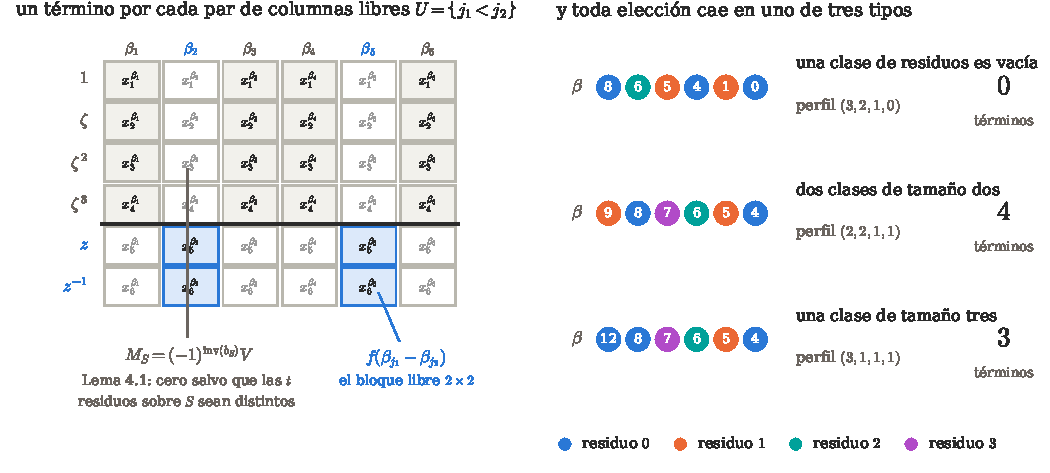
\includegraphics[width=\textwidth]{fig_laplace_es.pdf}
\caption{La arquitectura de la demostración, dibujada con $t=4$, $N=6$. \emph{Izquierda:} el
determinante $\det(x_i^{\beta_j})$ desarrollado por las $t$ filas congeladas. Cada elección de las
dos columnas $U=\{j_1<j_2\}$ que se dejan a las filas libres $z,z^{-1}$ deja un menor $t\times t$
$M_S$ sobre las columnas complementarias, que por el Lema \ref{lem:L1} vale $\pm V$ o cero, por el
bloque $2\times2$ $f(\beta_{j_1}-\beta_{j_2})$. \emph{Derecha:} por el recuento del exceso dos
\eqref{eq:excess} sólo hay tres perfiles de residuos, uno por fila, cada uno sobre un beta-conjunto
que lo realiza; el número de la derecha es cuántas elecciones de $U$ sobreviven, contado y no
afirmado --- $0$, $4$ y $3$, que es la tricotomía sobre la que se organiza la sección. El color es
la clase de residuos. Calculada por \texttt{anc/fig\_proof.py}.}
\label{fig:laplace}
\end{figure}

El desarrollo en sí es el movimiento habitual de esta literatura y no reclamamos nada por él: Albion
\cite{Alb25} aplica el desarrollo de Laplace a un determinante de esta forma \emph{según la
estructura de bloques dada}, manteniendo fijo un primer conjunto de filas, siguiendo a Krattenthaler
y a Ciucu--Krattenthaler. Lo particular aquí no es el desarrollo, sino con qué se topa.

Lo que el argumento hace en realidad es clasificar, no calcular. Desarrollar por las $t$ filas
congeladas deja un término por cada manera de elegir qué dos columnas \emph{no} lo están, y el
recuento del exceso dos dice que toda elección cae en exactamente uno de tres tipos combinatorios:
no sobrevive ninguna (una clase de residuos es vacía), sobreviven cuatro (dos clases de tamaño dos) o
sobreviven tres (una clase de tamaño tres). Todo lo que sigue es contabilidad dentro de un tipo, y el
Lema \ref{lem:L5} muestra que los dos últimos son un mismo enunciado visto dos veces. La Figura \ref{fig:laplace} es esa frase dibujada.

\begin{lemma}\label{lem:L1}
Sea $S$ un conjunto de $t$ columnas y $M_S=\det(\zeta^{k\beta_j})_{0\le k<t,\,j\in S}$. Entonces
$M_S=0$ salvo que los residuos $\{\beta_j\bmod t:j\in S\}$ sean dos a dos distintos, en cuyo caso
$M_S=(-1)^{\inv(b_S)}V$.
\end{lemma}

\begin{proof}
Como $\zeta^{k\beta_j}=(\zeta^{\beta_j})^k$, la matriz es de Vandermonde en los valores
$y_j=\zeta^{\beta_j}$, cuyo determinante es $\prod_{j<j'}(y_{j'}-y_j)$. El valor $y_j$ depende de
$\beta_j$ solo módulo $t$, luego dos columnas de $S$ que compartan residuo anulan el determinante. Si
los residuos son dos a dos distintos, $|S|=t$ obliga a $\{y_j\}_{j\in S}=\zt$ como conjunto, y el
determinante de Vandermonde es alternante en sus argumentos, luego vale $V$ por el signo de la
permutación que ordena $b_S$ crecientemente, que es $(-1)^{\inv(b_S)}$.
\end{proof}

\begin{lemma}\label{lem:L2}
$\det\bigl(x_i^{N-j}\bigr)_{i,j=1}^{N}=(-1)^{\binom t2}\,V\,(z^t-1)(z^{-t}-1)(z-z^{-1})$ para el
alfabeto $x=(1,\zeta,\dots,\zeta^{t-1},z,z^{-1})$ en ese orden.
\end{lemma}

\begin{proof}
El determinante es $\prod_{i<i'}(x_i-x_{i'})$. Los pares dentro de $\zt$ aportan
$\prod_{k<k'}(\zeta^k-\zeta^{k'})=(-1)^{\binom t2}V$; los pares $(\zeta^k,z)$ aportan
$\prod_k(\zeta^k-z)=(-1)^t(z^t-1)$ y los pares $(\zeta^k,z^{-1})$ aportan $(-1)^t(z^{-t}-1)$; el
último par aporta $z-z^{-1}$. Los dos factores $(-1)^t$ se cancelan.
\end{proof}

\noindent Lo calculamos porque son tres líneas, no porque sea desconocido: un determinante sobre un
alfabeto cerrado bajo $x\mapsto x^{-1}$, evaluado en forma de producto cerrado, es exactamente el
asunto del complemento de Krattenthaler al cálculo de determinantes \cite[\S5.11]{KratADCC}, cuyo
Lema 20 lleva entre sus casos particulares las fórmulas del denominador de Weyl para $B_n$, $C_n$ y
$D_n$. Lo que esa literatura no evalúa ---y lo que el lema siguiente necesita--- es ese mismo
determinante con una órbita de raíces de la unidad dentro del alfabeto.

\begin{lemma}\label{lem:L3}
Sea $\mathcal U$ el conjunto de pares $U=\{j_1<j_2\}$ de columnas cuyo complementario $S_U$ lleva las
$t$ clases de residuos. Entonces
\[
\Phi_t(\lambda;z)=\frac{(-1)^{\,t+\binom{N+1}{2}}}{(z^t-1)(z^{-t}-1)(z-z^{-1})}
\sum_{U\in\mathcal U}(-1)^{\,j_1+j_2+\inv(b_{S_U})}\,f(\beta_{j_1}-\beta_{j_2}).
\]
\end{lemma}

\begin{proof}
Desarrollando el numerador por Laplace a lo largo de las primeras $t$ filas,
\[
\det\bigl(x_i^{\beta_j}\bigr)=\sum_{|S|=t}(-1)^{\binom{t+1}{2}+\sum_{j\in S}j}\,M_S\,C_{S^c},
\]
donde para $S^c=\{j_1<j_2\}$ el menor complementario $2\times2$ es
$z^{\beta_{j_1}-\beta_{j_2}}-z^{-(\beta_{j_1}-\beta_{j_2})}=f(\beta_{j_1}-\beta_{j_2})$. Por el Lema
\ref{lem:L1} solo contribuyen los $S$ con residuos dos a dos distintos. Escribiendo
$\sum_{j\in S}j=\binom{N+1}{2}-j_1-j_2$ y dividiendo por el Lema \ref{lem:L2}, los factores $V$ se
cancelan y $(-1)^{\binom{t+1}{2}-\binom{t}{2}}=(-1)^t$.
\end{proof}

Si algún $n_i=0$, ningún $S$ de tamaño $t$ lleva todos los residuos, $\mathcal U=\varnothing$ y
$\Phi_t=0$: es el Teorema \ref{thm:main}(i). En caso contrario todos los $n_i\ge1$ y por
\eqref{eq:excess} o bien dos clases tienen tamaño dos, y entonces $S_U$ debe descartar un elemento de
cada una y $|\mathcal U|=4$, o bien una clase tiene tamaño tres, y entonces $S_U$ descarta dos de los
tres y $|\mathcal U|=3$.

\begin{lemma}[el movimiento de columna]\label{lem:L4}
Sean $A$ y $B$ clases distintas de tamaño dos, en las columnas $j_{A_1}<j_{A_2}$ y
$j_{B_1}<j_{B_2}$. Para $i,j\in\{1,2\}$ sea $U_{ij}$ el par formado por la columna de $a_i$ y la de
$b_j$, y sea $\kappa_{ij}=(-1)^{\,j_{A_i}+j_{B_j}+\inv(b_{S_{U_{ij}}})}\sgn(a_i-b_j)$, de modo que
el término $U_{ij}$ del Lema \ref{lem:L3} vale $\kappa_{ij}f(a_i-b_j)$. Entonces
$\kappa_{ij}=\kappa_{11}(-1)^{i-1}(-1)^{j-1}$.
\end{lemma}

\begin{proof}
Fijemos $j$ y comparemos $i=1$ con $i=2$. Los conjuntos $S_{U_{1j}}$ y $S_{U_{2j}}$ difieren solo en
que el primero contiene la columna $j_{A_2}$ y el segundo la columna $j_{A_1}$, y la letra que llevan
es el residuo $r_A$ en ambos casos. Pasar de una palabra a la otra mueve esa letra a través de
exactamente las columnas conservadas estrictamente entre $j_{A_1}$ y $j_{A_2}$, y ninguna de esas
letras es igual a $r_A$ porque la clase $A$ tiene solo dos elementos; cada cruce cambia la paridad de
$\inv$. Por tanto
\[
(-1)^{\inv(b_{S_{U_{1j}}})-\inv(b_{S_{U_{2j}}})}
=(-1)^{(j_{A_2}-j_{A_1}-1)-[\,a_2<b_j<a_1\,]},
\]
usando que $\beta$ es estrictamente decreciente en el índice de columna, de modo que $j_{B_j}$ está
estrictamente entre $j_{A_1}$ y $j_{A_2}$ exactamente cuando $a_2<b_j<a_1$. Multiplicando por el
factor de Laplace $(-1)^{j_{A_1}+j_{A_2}}$,
\[
\frac{\kappa_{1j}}{\kappa_{2j}}
=(-1)^{2j_{A_2}-1}(-1)^{[\,a_2<b_j<a_1\,]}\sgn(a_1-b_j)\sgn(a_2-b_j)=-1,
\]
porque $\sgn(a_1-b_j)\sgn(a_2-b_j)=-1$ exactamente cuando $b_j$ está entre $a_2$ y $a_1$.
Intercambiando los papeles de $A$ y $B$ se obtiene $\kappa_{i1}/\kappa_{i2}=-1$.
\end{proof}

\begin{lemma}\label{lem:L5}
Para todos $c,p,q$ y todos $u,v$,
\begin{align*}
\text{\rm(a)}&\quad \sum_{\epsilon,\eta\in\{\pm1\}}\epsilon\eta\,f(c+\epsilon p+\eta q)=f(c)f(p)f(q),\\
\text{\rm(b)}&\quad f(2u)-f(2u+2v)+f(2v)=-f(u)f(v)f(u+v).
\end{align*}
\end{lemma}

\begin{proof}
Para (a), $\sum_{\epsilon,\eta}\epsilon\eta\,z^{c+\epsilon p+\eta q}
=z^{c}\bigl(\sum_\epsilon\epsilon z^{\epsilon p}\bigr)\bigl(\sum_\eta\eta z^{\eta q}\bigr)
=z^{c}f(p)f(q)$, y el mismo cálculo para los exponentes negativos da $z^{-c}(-f(p))(-f(q))$;
réstese. Para (b), pónganse $s=z^u$, $w=z^v$ y desarróllese
$(s-s^{-1})(w-w^{-1})(sw-s^{-1}w^{-1})$: los ocho términos se recombinan como
$(s^2w^2-s^{-2}w^{-2})-(s^2-s^{-2})-(w^2-w^{-2})=f(2u+2v)-f(2u)-f(2v)$.
\end{proof}

\begin{proof}[Demostración del Teorema \ref{thm:main}]
En el perfil de dos clases, los Lemas \ref{lem:L3} y \ref{lem:L4} dan
\[
\sum_{U\in\mathcal U}(\cdots)=\kappa_{11}\sum_{i,j}(-1)^{i-1}(-1)^{j-1}f(a_i-b_j).
\]
Escribiendo $a_i=\alpha+\epsilon_ip$ y $b_j=\gamma+\eta_jq$ con $p=d_1/2$, $q=d_2/2$ y
$\epsilon=\eta=(+1,-1)$, se tiene $a_i-b_j=c+\epsilon_ip-\eta_jq$ con $c=\alpha-\gamma$. Sustituyendo
$\eta$ por $-\eta$, la suma se convierte en
$-\sum_{\epsilon,\eta}\epsilon\eta f(c+\epsilon p+\eta q)$, que vale $-f(c)f(p)f(q)$ por el Lema
\ref{lem:L5}(a). Como $(z^t-1)(z^{-t}-1)=2-z^t-z^{-t}=-f(t/2)^2$ y $z-z^{-1}=f(1)$, los dos signos
menos se cancelan, y sustituyendo $f(u)=2\sinh(u\theta)$ los factores numéricos se cancelan. Aquí
$2c=\tilde d_3$. Si $\tilde d_3=0$, entonces $f(c)=0$ y la suma entera se anula, que es la primera
afirmación de {\rm(ii)}; en caso contrario
$\sinh(c\theta)=\sgn(\tilde d_3)\sinh(d_3\theta/2)$, lo que da \eqref{eq:main} con
$\varepsilon_\lambda=(-1)^{\,t+\binom{N+1}{2}}\kappa_{11}\sgn(\tilde d_3)$, que es
\eqref{eq:sign} por la definición de $\kappa_{11}$ en el Lema \ref{lem:L4}.

Para el perfil de tamaño tres $\{p>q>r\}$ en las columnas $j_1<j_2<j_3$ se aplica el mismo argumento
de movimiento de columna, de nuevo porque ninguna letra estrictamente entre dos de esas columnas
lleva el residuo de la clase, y da signos alternantes $(\varsigma,-\varsigma,\varsigma)$ para los
tres términos $f(p-q)$, $f(p-r)$, $f(q-r)$. Por el Lema \ref{lem:L5}(b) con $u=(p-q)/2$,
$v=(q-r)/2$ la suma es $-\varsigma f(u)f(v)f(u+v)$, que es la fórmula de dos clases para $A=\{p,q\}$,
$B=\{q,r\}$ con $\varsigma=\kappa_{11}$. Equivalentemente, la cuarta selección ausente del perfil de
dos clases descartaría $q$ dos veces y su término lleva $f(0)=0$, de modo que los dos perfiles son un
solo enunciado.
\end{proof}

Todos los enunciados de este artículo se comprobaron además numéricamente; los recuentos se recogen
una sola vez, en la \S\ref{sec:verif}, en lugar de repetirse según van surgiendo.

%======================================================================
\section{Independencia en el lugar recíproco}\label{sec:independence}

El Teorema 5.3 de \cite{AK25} está enunciado para variables libres, y $(z,\zb)$ no es un par libre.
Nada de esta sección lo contradice: el lugar recíproco queda fuera de sus hipótesis, no en contra de
ellas, y lo que hacemos aquí es determinar en qué se convierte allí su criterio. Leída al pie de la
letra, \eqref{eq:AK53} diría que para $\ell(\lambda)\le2$ se tiene
$s_\lambda(z,\zb,\zt)=s_\lambda(z,\zb)$ exactamente sobre los $t$-núcleos. El Teorema
\ref{thm:main} evalúa el miembro izquierdo para toda $\lambda$, y al comparar ambos se ve que el
lugar recíproco lleva más soluciones: exactamente una familia. Medir cuánto sobrevive un criterio a
una degeneración es una manera de decir lo afilado que era, y la respuesta aquí es que lo es salvo
una sola familia.

Aislamos primero cuándo $\Phi_t$ degenera en un solo carácter.

\begin{lemma}\label{lem:single}
$\Phi_t(\lambda;z)=\pm\chi_k(z)$ para algún $k\ge0$ si y solo si el multiconjunto $\{d_1,d_2,d_3\}$
contiene $t$ al menos dos veces, y en tal caso la entrada restante vale $2(k+1)$.
\end{lemma}

\begin{proof}
Pongamos $u=z^{1/2}$, de modo que $2\sinh(d_i\theta/2)=u^{d_i}-u^{-d_i}$,
$2\sinh(t\theta/2)=u^{t}-u^{-t}$ y $2\sinh\theta=u^{2}-u^{-2}$; todos los exponentes son enteros. Por
\eqref{eq:main}, la igualdad afirmada es
\[
\prod_{i=1}^{3}\bigl(u^{d_i}-u^{-d_i}\bigr)
=\pm\bigl(u^{t}-u^{-t}\bigr)^{2}\bigl(u^{2k+2}-u^{-2k-2}\bigr).
\]
Usando $u^{n}-u^{-n}=u^{-n}(u^{2n}-1)$ en cada factor y comparando los prefactores monomiales se
obtiene $d_1+d_2+d_3=2t+2(k+1)$ junto con
\[
\prod_{i=1}^{3}\bigl(u^{2d_i}-1\bigr)=\pm\bigl(u^{2t}-1\bigr)^{2}\bigl(u^{4(k+1)}-1\bigr),
\]
y evaluando en $u=0$ el signo queda fijado en $+$. Ahora $u^{2n}-1=\prod_{m\mid 2n}Q_m(u)$ con
$Q_m$ los polinomios ciclotómicos como en la Proposición \ref{prop:minimal}, que son irreducibles y
distintos dos a dos, de modo que por
factorización única en $\ZZ[u]$ ambos miembros tienen el mismo multiconjunto de factores
ciclotómicos. A la izquierda ese multiconjunto es $\biguplus_i\{m:m\mid 2d_i\}$ y a la derecha
$2\times\{m:m\mid 2t\}\uplus\{m:m\mid 4(k+1)\}$. Su mayor elemento es $\max_i 2d_i$ a la izquierda y
$\max(2t,4(k+1))$ a la derecha; borrando de ambos lados el conjunto de divisores de ese máximo y
repitiendo dos veces más se llega a
\[
\{2d_1,2d_2,2d_3\}=\{2t,\,2t,\,4(k+1)\}
\]
como multiconjuntos, que es lo afirmado. El recíproco es el mismo cálculo leído al revés.
\end{proof}

\begin{theorem}\label{thm:extra}
Sea $\ell(\lambda)\le2$. Entonces
\[
\Phi_t(\lambda;z)=s_\lambda(z,\zb)
\]
---una igualdad, y no una igualdad salvo signo--- si y solo si o bien
$\lambda=\core_t(\lambda)$, o bien
\begin{equation}\label{eq:extra}
t\ \text{es par}\quad\text{y}\quad \lambda=\Bigl(\lambda_2+\tfrac{3t}{2}-1,\ \lambda_2\Bigr)
\quad\text{con}\quad \tfrac t2\le\lambda_2\le t-1 .
\end{equation}
En el segundo caso $\{d_1,d_2,d_3\}=\{3t,t,t\}$ y $\varepsilon_\lambda=+1$, mientras que
$\core_t(\lambda)=\bigl(\tfrac t2-1+j,j\bigr)$ y $\quot_t(\lambda)$ tiene como única componente no
vacía $(2)$, en la posición $j=\lambda_2-\tfrac t2$.
\end{theorem}

La Figura \ref{fig:locus} es el enunciado computado en vez de afirmado: ambas familias están
dibujadas sobre un rango de $t$, y el $t$ impar donde \eqref{eq:extra} no puede darse es el control.

\begin{figure}[!ht]
\centering
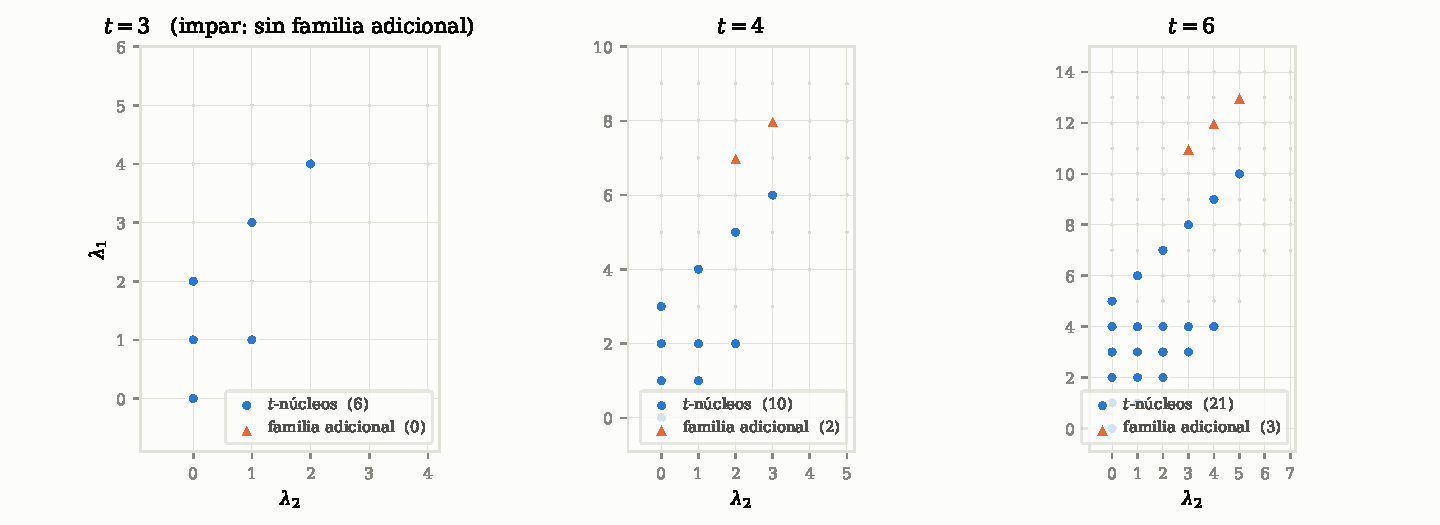
\includegraphics[width=\textwidth]{fig_locus_es.pdf}
\caption{El Teorema \ref{thm:extra}, calculado y no afirmado. Para toda $\lambda$ de dos filas en
rango se evaluaron ambos miembros de $\Phi_t(\lambda;z)=\pm s_\lambda(z,\zb)$; se representan las
particiones donde coinciden, coloreadas por familia. Los círculos son los $t$-núcleos, las soluciones
ya descritas por \eqref{eq:AK53}; los triángulos son la familia adicional \eqref{eq:extra}, que crea
la especialización recíproca. El caso impar $t=3$ es el control: por el Teorema \ref{thm:extra} allí
no puede existir solución adicional, y no se halla ninguna.}
\label{fig:locus}
\end{figure}

\begin{proof}
Como $\ell(\lambda)\le 2$ y $N=t+2$, el conjunto beta es
$\beta(\lambda)=\bigl(A'+t,\;B'+t,\;t-1,t-2,\dots,1,0\bigr)$ donde
\[
A':=\lambda_1+1,\qquad B':=\lambda_2,\qquad A'>B'\ge0 .
\]
El bloque $\{0,1,\dots,t-1\}$ toca cada clase de residuos exactamente una vez, luego ninguna clase es
vacía y las dos partes grandes deciden el perfil. Escribamos $A'=t\alpha+\rho_A$ y
$B'=t\gamma+\rho_B$ con $0\le\rho_A,\rho_B\le t-1$. Como $s_\lambda(z,\zb)=\chi_{\lambda_1-\lambda_2}(z)$,
el Lema \ref{lem:single} dice que la afirmación se cumple exactamente cuando $\{d_1,d_2,d_3\}$
contiene $t$ dos veces y la tercera entrada es $2(\lambda_1-\lambda_2+1)=2(A'-B')$.

\emph{Caso $\rho_A=\rho_B=:\rho$.} Una clase tiene tamaño tres, a saber $\{A'+t,B'+t,\rho\}$, y por el
Teorema \ref{thm:main} los tres argumentos son $d_1=A'-B'$, $d_2=B'+t-\rho=t(\gamma+1)$,
$d_3=A'+t-\rho=t(\alpha+1)$. Aquí $t\mid A'-B'$, digamos $A'-B'=ts$ con $s\ge1$. El par $d_2=d_3=t$
fuerza $\alpha=\gamma=0$, luego $A'=B'$, excluido. El par $d_1=d_3=t$ fuerza $s=1$ y $\alpha=0$,
luego $A'<t$ y $A'=B'+t\ge t$, excluido. El par $d_1=d_2=t$ fuerza $s=1$ y $\gamma=0$, es decir
$A'=B'+t$ con $B'<t$; entonces $\alpha=1$ y la tercera entrada es $d_3=2t=2(A'-B')$, como se
requiere. Este caso aporta pues exactamente las $\lambda$ con $A'=B'+t$, $B'<t$.

\emph{Caso $\rho_A\ne\rho_B$.} Dos clases tienen tamaño dos, a saber $\{A'+t,\rho_A\}$ y
$\{B'+t,\rho_B\}$, y los tres argumentos son
\[
d_A=t(\alpha+1),\qquad d_B=t(\gamma+1),\qquad
d_3=\bigl|\,t(\alpha-\gamma)+2(\rho_A-\rho_B)\,\bigr| .
\]
Si $d_A=d_B=t$ entonces $\alpha=\gamma=0$, luego $A',B'<t$ y $d_3=2|\rho_A-\rho_B|=2(A'-B')$
automáticamente: toda tal $\lambda$ es solución. En otro caso exactamente uno de $d_A,d_B$ vale $t$ y
$d_3=t$. Si $\alpha=0$ y $\gamma\ge1$, entonces $|-t\gamma+2(\rho_A-\rho_B)|=t$ con
$|\rho_A-\rho_B|\le t-1$ fuerza $\gamma=2$ y $\rho_A-\rho_B=t/2$; pero entonces
$\lambda_1=A'-1=\rho_A-1<t$ mientras que $\lambda_2=B'\ge2t$, en contra de $\lambda_1\ge\lambda_2$.
Si $\gamma=0$ y $\alpha\ge1$, entonces $|t\alpha+2(\rho_A-\rho_B)|=t$ fuerza, para $\alpha=1$,
$\rho_A=\rho_B$ (excluido), y para $\alpha=2$,
\[
\rho_B-\rho_A=\tfrac t2,
\]
lo que exige $t$ par; $\alpha\ge3$ da $|2(\rho_A-\rho_B)|\ge2t$, imposible. Luego $A'=2t+\rho_A$,
$B'=\rho_B=\rho_A+\tfrac t2$, de donde
\[
\lambda_1=2t+\rho_A-1,\qquad \lambda_2=\rho_A+\tfrac t2,\qquad
\lambda_1-\lambda_2=\tfrac{3t}{2}-1,
\]
y $\rho_B\le t-1$ da $0\le\rho_A\le\tfrac t2-1$, es decir $\tfrac t2\le\lambda_2\le t-1$. La entrada
restante es $d_A=t(\alpha+1)=3t=2(\lambda_1-\lambda_2+1)$, como se requiere. Esto es
\eqref{eq:extra}.

Queda identificar las soluciones del primer caso de cada análisis con los $t$-núcleos. Para
$\ell(\lambda)\le2$ el conjunto beta en dos posiciones es $(A',B')$, y $\lambda$ es un $t$-núcleo si
y solo si ningún número beta puede rebajarse en $t$ hasta una posición no negativa desocupada, es
decir si y solo si $B'<t$ y o bien $A'<t$ o bien $A'=B'+t$. Son exactamente las dos familias
halladas. Por último, en el caso \eqref{eq:extra} la clase $\rho_A$ lleva $\{2t+\rho_A+t,\rho_A\}$,
luego su componente del cociente es $(2)$, toda otra componente es vacía, y el núcleo es el
enunciado.

\emph{El signo.} Las dos familias lo consiguen por razones distintas. Sobre los $t$-núcleos la
igualdad es \eqref{eq:AK53} misma, que es una igualdad y no una igualdad salvo signo, así que no hay
nada que probar. Sobre \eqref{eq:extra}, escríbase $t=2m$ y $\lambda_2=m+j$ con $0\le j\le m-1$, de
modo que $\rho_A=j$ y $\rho_B=m+j$ y
\[
\beta(\lambda)=\bigl(6m+j,\;3m+j,\;2m-1,2m-2,\dots,1,0\bigr).
\]
Reduciendo módulo $t=2m$, la palabra de residuos leída en orden creciente de columna es
\[
w=\bigl(j,\;m+j,\;2m-1,2m-2,\dots,1,0\bigr),
\]
puesto que $6m+j\equiv j$ y $3m+j\equiv m+j$, esto último porque $j\le m-1$. Sus inversiones son de
tres clases: la cola decreciente aporta $\binom{2m}{2}$; la primera letra está por encima de
exactamente las $j$ letras de la cola $0,\dots,j-1$; la segunda, por encima de exactamente las $m+j$
letras $0,\dots,m+j-1$; y las dos primeras letras están en orden creciente, así que no aportan
ninguna. Por tanto
\begin{equation}\label{eq:extrainv}
\inv(w)=\binom{2m}{2}+j+(m+j)=2m^{2}+2j\;\equiv\;0\pmod2 ,
\end{equation}
luego $\sgn(\sigma)=(-1)^{\inv(w)}=+1$ por la primera línea de la prueba de la Proposición
\ref{rem:sign}. Las dos clases distinguidas son $r_A=j<r_B=m+j$, que llevan $A=\{6m+j,\,j\}$ y
$B=\{3m+j,\,m+j\}$, de modo que $\tilde d_3=(6m+2j)-(4m+2j)=2m>0$ y $\sgn(\tilde d_3)=+1$. Los dos
factores restantes de \eqref{eq:shortsign} son $(-1)^{\lfloor t/2\rfloor}=(-1)^{m}$ y
$(-1)^{r_A+r_B}=(-1)^{m+2j}=(-1)^{m}$, cuyo producto es $+1$. Así pues $\varepsilon_\lambda=+1$, y
como $d_1=6m=3t$, $d_2=2m=t$ y $d_3=2m=t$, \eqref{eq:main} dice
\[
\Phi_t(\lambda;z)=\frac{\sinh(3t\theta/2)\sinh^{2}(t\theta/2)}{\sinh^{2}(t\theta/2)\sinh\theta}
=\chi_{\frac{3t}{2}-1}(z)=\chi_{\lambda_1-\lambda_2}(z)=s_\lambda(z,\zb),
\]
sin ningún signo que arrastrar.
\end{proof}

\noindent Lo que compra \eqref{eq:extrainv} no es decoración. Enunciado salvo signo, el Teorema
\ref{thm:extra} dice que la especialización crea una familia de formas sobre las que el twist es
invisible \emph{salvo un signo}, que es un enunciado más débil que el que \eqref{eq:AK53} hace sobre
los núcleos; con el signo resuelto, las dos familias son soluciones de la misma ecuación, y ``el
lugar recíproco adquiere exactamente una familia más'' es literalmente cierto.

\begin{remark}\label{rem:why}
El Lema \ref{lem:single} controla el valor sólo salvo signo, y por eso el signo del Teorema
\ref{thm:extra} necesita el párrafo aparte de arriba en lugar de salir de la clasificación.

La familia adicional pertenece a la especialización y no al alfabeto. El paso es el
\cite[Lema 5.2]{AK25}, sobre el que se apoya el \cite[Teorema 5.3]{AK25}: reduce la independencia a
la anulación de $s_{\lambda/\mu}$ en el alfabeto torcido para todo $\mu\subsetneq\lambda$, y la
reducción usa la independencia lineal de los caracteres universales $f_\mu$ en las variables libres. En el lugar recíproco
$s_\mu(z,\zb)=\chi_{\mu_1-\mu_2}(z)$ depende solo de $\mu_1-\mu_2$, luego $s_{(1)}$, $s_{(2,1)}$ y
$s_{(3,2)}$ coinciden allí y esa independencia deja de estar disponible; el Teorema \ref{thm:extra}
mide la diferencia. Un control confirma la lectura: para $\lambda=(3,1)$ y $t=2$ se tiene
$s_\lambda(\zt,z,\zb)=s_\lambda(z,\zb)$, mientras que $s_\lambda(\zt,x,y)\ne s_\lambda(x,y)$ para
$x,y$ libres.
\end{remark}

Así pues, el criterio no sobrevive intacto a la especialización, y lo que adquiere es pequeño y
nombrable: una familia, para formas de dos filas, indexada por un elemento de orden dos del retículo
de residuos y clasificada por su núcleo y su cociente. Las soluciones adicionales pertenecen al lugar
recíproco y no al alfabeto ---existen porque una especialización ha retirado una independencia lineal
que el argumento original usaba, y ese paso que falta es exactamente lo que mide el Teorema
\ref{thm:extra}.

%======================================================================
\section{Una enumeración en la que sobrevive un parámetro}\label{sec:enum}

Desarrollando $s_\lambda$ sobre tablas semiestándar, el Teorema \ref{thm:main} se convierte en una
fórmula de producto para un recuento pesado. Sea $m_k(T)$ el número de entradas iguales a $k$ en $T$.

\begin{corollary}\label{cor:enum}
Desarrollando $s_\lambda$ sobre tablas semiestándar y aplicando el Teorema \ref{thm:main}: para todo
$t\ge2$ y toda $\lambda\in\PP_{t+2}$,
\[
\sum_{T\in\mathrm{SSYT}(\lambda,\,t+2)}
\zeta^{\,\sum_{k=1}^{t}(k-1)m_k(T)}\;z^{\,m_{t+1}(T)-m_{t+2}(T)}
\;=\;\varepsilon_\lambda\,
\frac{\sinh(d_1\theta/2)\sinh(d_2\theta/2)\sinh(d_3\theta/2)}{\sinh^2(t\theta/2)\sinh\theta}.
\]
\end{corollary}

Para $t=2$ el peso es $(-1)^{m_2(T)}$, y si $\lambda=(c^{\,a})$ es rectangular entonces
$\mathrm{SSYT}(\lambda,4)$ está en biyección con las particiones planas en una caja
$a\times(4-a)\times c$, equivalentemente con las teselaciones de rombos de un hexágono. El Corolario
\ref{cor:enum} es entonces una $(-1)$-enumeración de esos objetos \emph{refinada por un parámetro
libre} $z$, que registra la diferencia entre los números de entradas $3$ y $4$. Poniendo $z=1$ se
recupera el recuento con signo puro, que por \eqref{eq:main} vale $\pm d_1d_2d_3/(2t^2)$: para la
$a=2$, $c=2$ vale $4$; para $a=2$, $c=4$ vale $9$; para $a=3$, $c=3$ vale $-6$.

\begin{example}\label{ex:boxes}
Tomando $\lambda=(c^{\,a})$ con $1\le a\le4$ y $t=2$, la forma tiene a lo sumo cuatro filas, las
tablas son las particiones planas en una caja $a\times(4-a)\times c$, y la forma cerrada da los
recuentos con signo de la Figura \ref{fig:signed}. Leyéndola:
\[
\begin{array}{ll}
1\times3\times c: & \bigl\lfloor (c+2)^2/4\bigr\rfloor,\\[2pt]
2\times2\times c: & (c/2+1)^2 \text{ si } c \text{ es par},\qquad 0 \text{ si } c \text{ es impar},\\[2pt]
3\times1\times c: & (-1)^c\bigl\lfloor (c+2)^2/4\bigr\rfloor,\\[2pt]
4\times0\times c: & (-1)^c .
\end{array}
\]
La tercera fila es la traspuesta de la primera, y por eso los módulos coinciden; la cuarta es la caja
degenerada, donde $s_{(c^4)}(x)=(x_1x_2x_3x_4)^c$ y el alfabeto tiene determinante $-1$. No
reivindicamos estos recuentos concretos como nuevos ---las cajas son pequeñas y el signo aquí es la
especialización $x_2=-1$, no el signo de complementación de las $(-1)$-enumeraciones de Kuperberg---
y los registramos solo para mostrar lo que produce el teorema. Lo que sí parece nuevo es que cada uno
de ellos es el valor en $z\mapsto1$ de un refinamiento de un parámetro con la misma fórmula de
producto.
\end{example}

Los cuadrados perfectos del Ejemplo \ref{ex:boxes} no son un accidente de casos pequeños: son lo que
la lectura por intervalos de la \S\ref{sec:intervals} dice que un rectángulo debe producir.

\begin{proposition}\label{prop:rect}
Sean $t=2$ y $\lambda=(c^{\,a})$ con $1\le a\le4$. Entonces uno de $d_1,d_2,d_3$ vale $2$, y:
\begin{enumerate}
\item[\rm(i)] si $a=4$, los tres valen $2$ sea cual sea $c$ y el recuento es $(-1)^c$: es el
rectángulo completo, donde $s_{(c^4)}(x)=(x_1x_2x_3x_4)^{c}$ se reduce a un monomio y del alfabeto no
queda más que su determinante;
\item[\rm(ii)] si $a\le3$ y $c$ es par, los otros dos valen ambos $c+2$, de modo que los dos
intervalos tienen \emph{la misma longitud} y el recuento con signo es el cuadrado perfecto
$\bigl(\tfrac{c+2}{2}\bigr)^2$;
\item[\rm(iii)] si $c$ es impar y $a=2$, los dos intervalos son \emph{concéntricos} y el recuento es
$0$;
\item[\rm(iv)] si $c$ es impar y $a\in\{1,3\}$, los otros dos valen $c+1$ y $c+3$, y el recuento es
$\pm\tfrac{(c+1)(c+3)}{4}=\pm\bigl\lfloor\tfrac{(c+2)^2}{4}\bigr\rfloor$.
\end{enumerate}
El caso {\rm(i)} no es una degeneración del triple de intervalos sino un colapso de la forma misma, y
es el único en el que la paridad de $c$ no interviene.
\end{proposition}

\begin{proof}
Para $\lambda=(c^{\,a})$ el conjunto beta consta de dos bloques de enteros consecutivos, a saber
$c+3,c+2,\dots,c+4-a$ y $3-a,2-a,\dots,0$; los residuos alternan a lo largo de cada bloque, y eso es
lo que fuerza las coincidencias. Explícitamente, para $a=1,2,3,4$ el conjunto beta es $(c+3,2,1,0)$,
$(c+3,c+2,1,0)$, $(c+3,c+2,c+1,0)$ y $(c+3,c+2,c+1,c)$. Separando cada uno por paridad se obtiene,
para $c$ par,
\[
\{c{+}3,1\},\{2,0\};\qquad \{c{+}3,1\},\{c{+}2,0\};\qquad \{c{+}3,c{+}1\},\{c{+}2,0\};\qquad
\{c{+}3,c{+}1\},\{c{+}2,c\},
\]
de donde $(d_1,d_2,d_3)$ vale $(c{+}2,2,c{+}2)$, $(c{+}2,c{+}2,2)$, $(2,c{+}2,c{+}2)$ y $(2,2,2)$
respectivamente; en cada caso el producto dividido por $2t^2=8$ es $\bigl(\tfrac{c+2}{2}\bigr)^2$,
resp. $1$. Para $c$ impar y $a=2$ la separación es $\{c{+}3,0\},\{c{+}2,1\}$, luego
$d_3=|c{+}3+0-c{-}2-1|=0$: los intervalos son concéntricos y se aplica el Corolario \ref{cor:zero}.
Para $c$ impar y $a=1,3$ la paridad pone tres números beta en una misma clase, $\{c{+}3,2,0\}$ y
$\{c{+}3,c{+}1,0\}$ respectivamente, y el perfil de tamaño tres da $(c{+}1,2,c{+}3)$ y
$(2,c{+}1,c{+}3)$, con producto dividido por $8$ igual a $\tfrac{(c+1)(c+3)}{4}$. Para $c$ impar y
$a=4$ los cuatro números beta vuelven a ser consecutivos, así que la separación es
$\{c{+}3,c{+}1\},\{c{+}2,c\}$ y el triple es $(2,2,2)$ igual que para $c$ par: a altura completa el
resultado no ve la paridad de $c$, y por eso $a=4$ va aparte.
\end{proof}

Así pues el cuadrado es el cuadrado de la mitad de la longitud común de los intervalos, los ceros son
las configuraciones concéntricas, los cuartos de cuadrado son el caso en que las dos longitudes
difieren en $2$, y a altura completa los tres intervalos coinciden, la forma se vuelve un monomio y no
sobrevive más que un signo. Qué par de los tres coincide rota con $a$, y por eso el mismo valor
reaparece en columnas distintas de la Figura \ref{fig:signed}.

\begin{figure}[t]
\centering
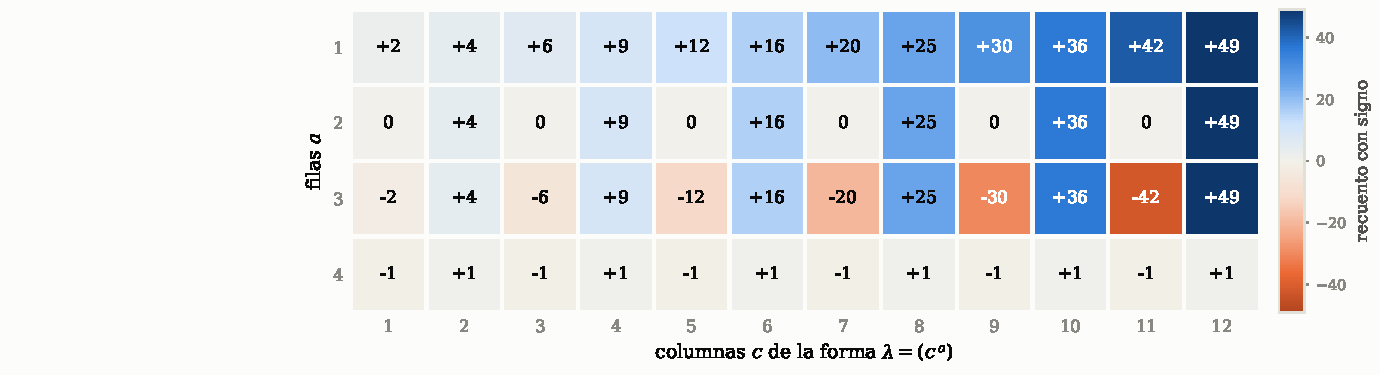
\includegraphics[width=\textwidth]{fig_signed_es.pdf}
\caption{Los recuentos con signo del Ejemplo \ref{ex:boxes}: el valor del Corolario \ref{cor:enum} en
$z=1$ y $t=2$ para las formas rectangulares $\lambda=(c^{\,a})$, esto es la $(-1)$-enumeración de
particiones planas en una caja $a\times(4-a)\times c$. Cada entrada es la forma cerrada
$\varepsilon_\lambda\,d_1d_2d_3/(2t^2)$, contrastada contra una enumeración directa de las tablas. La
fila $a=2$ se anula para $c$ impar y es un cuadrado perfecto para $c$ par.}
\label{fig:signed}
\end{figure}

La literatura de $(-1)$-enumeración calcula tales recuentos con signo, y conviene ser exacto en cómo,
porque la diferencia de aquí es estrecha. Kuperberg \cite{Kup02} pesa los objetos por $\pm1$
directamente. Eisenkölbl \cite{Eis07} especializa $x_i=(-1)^i$ en una identidad de funciones de Schur
del tipo que usó Stanley \cite{Sta86} ---identidad que allí se señala que es también
\cite[Cor.~7.3]{IOTZ06}--- y obtiene la $(-1)$-enumeración de las particiones planas
autocomplementarias con un lado impar. Ciucu y Krattenthaler evalúan los determinantes
correspondientes. En todos ellos el alfabeto es un número y no queda nada libre, que es el único
punto de diferencia: aquí el par recíproco mantiene viva una variable a lo largo del recuento con
signo. Eso lo hace el alfabeto, no un argumento nuestro.

En el mundo de las cintas hay un refinamiento de otra clase, y conviene decir cuál: los polinomios
LLT de Lascoux, Leclerc y Thibon \cite{LLT97} gradúan las tablas de cintas por un estadístico de
spin. Ese $q$ es una graduación añadida y no una letra, y el objeto que gradúa va indexado por una
tupla de formas; el parámetro de aquí es el del propio alfabeto y quien lo transporta es un solo
$s_\lambda$. Los dos refinan cosas distintas, y por eso enunciamos el punto de forma estrecha: es el
par recíproco, y no un estadístico, lo que mantiene viva una variable a través del recuento con
signo.

Una enumeración con signo que tiene fórmula de producto pide una involución que invierta el signo, y
el obstáculo es específico: la involución debe preservar $m_{t+1}-m_{t+2}$, o el parámetro libre no
se transporta, y ni los movimientos de Bender--Knuth ni el intercambio de una sola celda lo hacen.
La construcción de \cite{KumariThesis} de una involución sin puntos fijos que invierte el signo
sobre tablas semiestándar en un alfabeto emparejado por $\pm$, cuyo conjunto fijo son las tablas
embaldosables por dominós, sí tiene la propiedad requerida en su instancia $i=1$: toca solo celdas
que contienen $1$ o $2$, luego preserva $z^{m_3-m_4}$ e invierte $(-1)^{m_2}$. El producto triple
sobre el que tendría que aterrizar es el del Corolario \ref{cor:chars}, que en $t=2$ es sin más un
producto de tres caracteres $\mathfrak{sl}_2$, de modo que la biyección que falta es un enunciado de
Clebsch--Gordan. Esa es una mitad. La
otra es la cancelación a través de la partición del alfabeto, y en $t=2$ concierne a una única
familia de un parámetro. Por \eqref{eq:threestep} más abajo,
\[
s_\lambda(1,-1,z,\zb)=\sum_{\ell(\nu)\le2}s_{\lambda/\nu}(1,-1)\,\chi_{\nu_1-\nu_2}(z),
\]
y una involución que transporte el parámetro debe preservar $k=\nu_1-\nu_2$, porque ese es el índice
del carácter sobre el que se apoya su término. Para $k$ fijo las $\nu$ admisibles son exactamente
$(m+k,m)$ con $m\ge0$, de modo que esa cancelación es un enunciado sobre una sola palabra.

El tamaño de los términos es clásico. El teorema de Littlewood tiene forma sesgada ---$\varphi_t
s_{\lambda/\nu}$ se anula salvo que $\lambda/\nu$ sea embaldosable por $t$-cintas, y en otro caso es
un signo de cinta por un producto sobre el cociente---, debida a Macdonald \cite[p.~91]{Mac95} y
demostrada allí por la misma vía de Jacobi--Trudi que tomamos abajo; el caso en que $\nu$ es el
$t$-núcleo es de Farahat. En $t=2$ y sobre nuestro alfabeto da $\sigma_m\in\{0,\pm1\}$ de inmediato.
Lo que no es clásico es cómo se mueve el signo con $m$, y eso es lo que la involución necesita.

\begin{figure}[t]
\centering
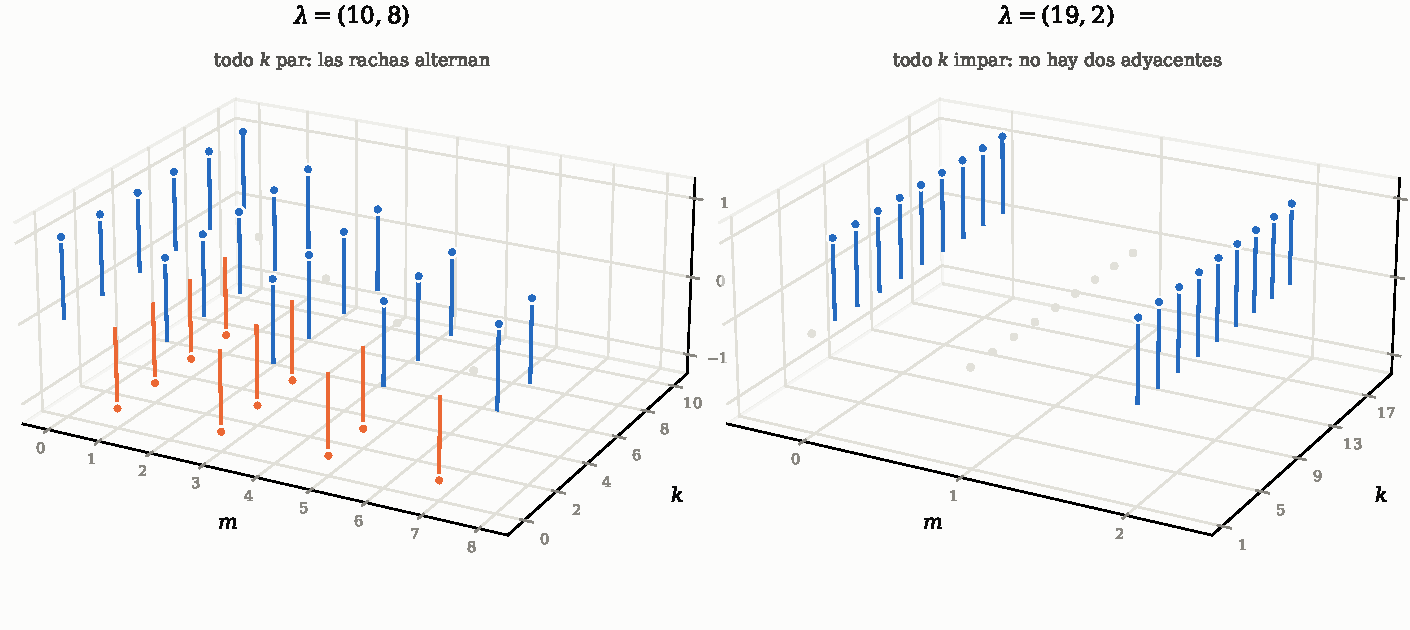
\includegraphics[width=\textwidth]{fig_runs_es.pdf}
\caption{La Proposición \ref{rem:involution}, dibujada. Para cada $k$ las $\nu$ admisibles son la
única familia $(m+k,m)$, y se representa $\sigma_m=s_{\lambda/(m+k,m)}(1,-1)$ frente a $m$ y $k$; los
puntos grises son los ceros. Toda barra tiene altura exactamente $\pm1$, que es la parte (i): los
términos forman un conjunto, luego la cancelación que pide la enumeración es un emparejamiento y no
algo con multiplicidad. A la izquierda todo $k$ es par y el color alterna a lo largo de cada racha,
que es la parte (iii) y lo que hace que $m\leftrightarrow m+1$ invierta el signo; donde una racha
acaba, la acaba un cero. A la derecha todo $k$ es impar y no hay dos términos no nulos contiguos,
que es la parte (ii): las rachas tienen longitud uno y no hay nada que cancelar.}
\label{fig:runs}
\end{figure}

\begin{proposition}[las rachas alternan]\label{rem:involution}
Sean $t=2$ y $k\ge0$, y sea $\sigma_m=s_{\lambda/(m+k,m)}(1,-1)$ para $m\ge0$. Entonces
\begin{enumerate}
\item[\rm(i)] $\sigma_m\in\{0,\pm1\}$ --- esta parte es de Macdonald y no nuestra;
\item[\rm(ii)] si $k$ es impar, no hay dos $\sigma_m$ consecutivos no nulos;
\item[\rm(iii)] si $\sigma_m$ y $\sigma_{m+1}$ son ambos no nulos, entonces
$\sigma_{m+1}=-\sigma_m$.
\end{enumerate}
En consecuencia, emparejar $m$ con $m+1$ dentro de cada racha maximal de $\sigma$ no nulos
consecutivos es una involución que invierte el signo, y $\sum_m\sigma_m$ es el recuento con signo de
las rachas de longitud impar.
\end{proposition}

Las tres partes se ven a la vez en la Figura \ref{fig:runs}: las alturas de las barras son la parte
{\rm(i)}, los huecos del panel impar son la parte {\rm(ii)}, y la alternancia del color a lo largo de
cada racha es la parte {\rm(iii)}.

\begin{proof}
Escribamos $\beta_i=\lambda_i-i$ y $c_j=\nu_j-j$, y tomemos la matriz de Jacobi--Trudi de
$s_{\lambda/\nu}$ con $n\ge\ell(\lambda)$ filas. Como $h_j(1,-1)=1$ para $j\ge0$ par y $0$ en otro
caso,
\begin{equation}\label{eq:betaJT}
M_{ij}=\bigl[\beta_i\ge c_j\bigr]\cdot\bigl[\beta_i\equiv c_j \bmod 2\bigr],\qquad
\sigma_m=\det M .
\end{equation}
El segundo factor dice que la columna $j$ está soportada en las filas de una sola clase de paridad,
la de $c_j$; y como $\beta_1>\dots>\beta_n$, dentro de esa clase el primer factor recorta un
\emph{segmento inicial}. Ordenando las filas por clase de paridad, $M$ queda diagonal por bloques,
de modo que es singular salvo que cada clase lleve tantas columnas como filas tiene, y dentro de una
clase es la escalera $\bigl[\,\text{el rango de }i\text{ en su clase}\le\ell_j\bigr]$ de las
longitudes $\ell_j$. Esa escalera es singular si dos longitudes coinciden o alguna es $0$, y en otro
caso las longitudes son una permutación de $1,\dots,e$ y su determinante es el signo de esa
permutación. Esto da (i), que en este caso es \cite[p.~91]{Mac95}; lo rededucimos porque la forma
$\beta$ \eqref{eq:betaJT} es lo que sostiene (ii) y (iii).

Para $\nu=(m+k,m)$ se tiene $c_1=m+k-1$, $c_2=m-2$ y $c_j=-j$ para $j\ge3$. Luego $c_1-c_2=k+1$, y
pasar de $m$ a $m+1$ sube $c_1$ y $c_2$ en uno y deja las demás columnas quietas: cambian de clase
de paridad exactamente las dos primeras.

Si $k$ es impar entonces $c_1\equiv c_2$, así que las columnas $1$ y $2$ están en la misma clase y
ambas la abandonan. El número de columnas de esa clase cambia en dos mientras que su número de filas
no, de modo que a lo sumo uno de $\sigma_m$, $\sigma_{m+1}$ puede ser no nulo, que es (ii).

Si $k$ es par entonces $c_1\not\equiv c_2$ y las dos columnas intercambian clase. Supongamos que
ambos son no nulos. En la clase de $c_1$ las columnas son la columna $1$ junto con un conjunto de
columnas $j\ge3$ que no se mueve; por (i) las longitudes son una permutación de $1,\dots,e$ antes y
después, y las columnas fijas aportan las mismas a ambas, luego la longitud que trae la columna $2$
es la que se llevó la columna $1$ ---y simétricamente en la otra clase. Cada clase ve por tanto las
mismas longitudes en el mismo orden de columnas, y los dos determinantes de bloque no cambian. Lo
que sí cambia es la baraja que separa las dos clases de columnas: las columnas $1$ y $2$ son
contiguas e intercambian pertenencia, lo que altera el número de inversiones de esa baraja en
exactamente uno. Luego $\sigma_{m+1}=-\sigma_m$, que es (iii).
\end{proof}

\begin{remark}[el signo de aquí es el signo del Teorema \ref{thm:main}]\label{rem:onesign}
Escribamos $\sigma_\nu$ para la permutación de la \S\ref{sec:background} asociada a una partición
$\nu$: la que ordena $\beta$ por clase de residuos, y que la Proposición \ref{rem:sign} coloca
dentro de $\varepsilon_\lambda$. Los términos de la Proposición \ref{rem:involution} son valores de
ese mismo signo. En efecto, $\sigma_m$ se anula salvo que $\core_2(\lambda)=\core_2(\nu)$ y ambas
componentes del $2$-cociente sesgado sean tiras horizontales, y vale
$\sgn(\sigma_\lambda)\sgn(\sigma_\nu)$ cuando no se anula ---siendo la identidad
$\sgn(\sigma_\lambda)\sgn(\sigma_\nu)=(-1)^{\sum_B\mathrm{ht}(B)}$ el signo de cintas de
\cite[p.~91]{Mac95} escrito como signo de ordenación, que es
\cite[Lema 6.3]{KumariThesis}. Las partes {\rm(ii)} y {\rm(iii)} son
entonces un único enunciado sobre $\sigma_\nu$ solo: al pasar $\nu=(m+k,m)$ a $(m+k+1,m+1)$,
$\sgn(\sigma_\nu)$ cambia de signo si $k$ es par y es constante si $k$ es impar. Así que la
permutación que lleva el signo del teorema principal es la permutación que hace alternar la
involución de esta sección; las dos mitades del artículo están firmadas por un mismo objeto.
\end{remark}

El emparejamiento es una biyección de tablas y no solo de términos, que es lo que transporta el
parámetro. Una tabla semiestándar de forma $(a,b)$ en las letras $3,4$ tiene segunda fila $4^{\,b}$
y primera fila $3^{\,p}4^{\,a-p}$ con $b\le p\le a$, de peso $z^{2p-a-b}$; añadirle una primera
columna $\left(\begin{smallmatrix}3\\4\end{smallmatrix}\right)$ la lleva a la tabla de forma
$(a+1,b+1)$ con $p+1$ en lugar de $p$, y $2(p+1)-(a+1)-(b+1)=2p-a-b$, de modo que $m_3-m_4$ se
preserva exactamente. Componer eso con la Proposición \ref{rem:involution} empareja los términos del
Corolario \ref{cor:enum} del modo que la enumeración pide.

Una mitad no es nuestra, y decimos cuál. La Proposición \ref{rem:involution} despacha la cancelación
a través de $\nu$; la cancelación \emph{dentro} de cada $s_{\lambda/\nu}(1,-1)$ es
\cite{KumariThesis}, y las dos encajan. Allí, con $n=1$, el alfabeto es $(x,-x)$ y el peso de un
llenado de dos letras es $(-1)^{c_2}$, que es $\sigma_m$; la involución
\cite[Lema 2.18]{KumariThesis} es libre de puntos fijos sobre los llenados \emph{no cubribles}, de
modo que la suma se reduce a los cubribles, que el \cite[Lema 2.16]{KumariThesis} pone en
correspondencia con tablas de dominó. Lo que hace utilizable la reducción aquí es el
\cite[Lema 2.14]{KumariThesis}: la paridad del número de dominós verticales no depende de la tabla,
luego toda superviviente lleva el mismo signo y $\sigma_m=\pm\#\{\text{llenados cubribles}\}$. Con la
parte (i), eso obliga al recuento a ser a lo sumo uno, así que el conjunto fijo es un único llenado
cuando $\sigma_m\ne0$ y vacío en otro caso ---comprobado directamente sobre las $1134$ formas
sesgadas con a lo sumo cuatro filas y $|\lambda|\le10$, donde los dos recuentos coinciden sin
excepción.

En $t=2$ existe por tanto la involución que la enumeración pide: cancelar dentro de cada $\nu$ por
el \cite[Lema 2.18]{KumariThesis}, emparejar lo que queda a través de $\nu$ por la Proposición
\ref{rem:involution}, y transportar el parámetro con la columna
$\left(\begin{smallmatrix}3\\4\end{smallmatrix}\right)$. Sus puntos fijos son un llenado por cada
racha de longitud impar, y el Corolario \ref{cor:enum} los cuenta. La construcción es de Kumari; el
ensamblaje es nuestro.

%======================================================================
\section{La factorización está aislada}\label{sec:sharp}

Una factorización solo es un resultado si no es especialización de otra conocida, y solo es un
resultado \emph{nítido} si el alfabeto no admite deformación. Eso no lo demostramos en general. Lo
que hacemos es probar cuatro deformaciones de \eqref{eq:object}, y las cuatro destruyen el producto.

La evidencia de esta sección es computacional, y así la etiquetamos: ninguna de (D1)--(D4) es un
teorema, y en particular no demostramos ningún resultado de imposibilidad. Lo que afirmamos es que la
identidad \eqref{eq:main} es falsa para cada alfabeto deformado, cosa que zanja un solo
contraejemplo, y damos recuentos para indicar cuán lejos está de ser cierta.

\begin{itemize}
\item[\rm(D1)] \emph{Más pares recíprocos.} Para
$s_\lambda(\zt,z_1,z_1^{-1},\dots,z_r,z_r^{-1})$
la ley de producto del Teorema \ref{thm:main} ya falla en $r=2$: en el rango calculado los valores
típicos llevan un factor irreducible grande, y los únicos
factores que se observa que se desprendan son binomios en las variables rotadas $z_1z_2$ y $z_1z_2^{-1}$, esto es,
los acoplamientos entre las cargas $u(1)$ de los pares. Lo que sí sobrevive es el \emph{lugar de
anulación}: en $t=2$ sobrevive a todo $r$ y el Teorema \ref{conj:crit} lo determina por completo,
mientras que para $t$ y $r$ arbitrarios el Teorema \ref{thm:suff} da un criterio suficiente uniforme
y la Conjetura \ref{conj:general} es el recíproco. Con esta evidencia el producto parece un accidente
de rango uno y la anulación la parte que generaliza; la primera mitad de esa frase es la Conjetura
\ref{conj:rank2} y sólo la segunda es un teorema.
\item[\rm(D2)] \emph{Más variables en la órbita.} Para
$s_\lambda(X,\zeta X,\dots,\zeta^{t-1}X,z,z^{-1})$ la ley de producto ya falla en $|X|=n=2$. Con $t=2$,
$n=2$ el valor para $\lambda=(2)$ es $(x^2z^2+y^2z^2+z^4+z^2+1)/z^2$, irreducible sobre $\mathbb Q$;
para $\lambda=(2,2)$ es $(x^2+y^2+z^2)(x^2z^2+y^2z^2+1)/z^2$, dos factores en lugar de tres; y para
$\lambda=(3,1)$ es de nuevo irreducible. En cambio, suprimido el par, el mismo alfabeto obedece
\cite[Teorema 2.3]{AK25}: $s_{(2)}(x,y,-x,-y)=x^2+y^2$ y $s_{(2,2)}(x,y,-x,-y)=(x^2+y^2)^2$.
\item[\rm(D3)] \emph{La órbita sustituida por una clase lateral.} Para $\zeta'\zt$ con
$\zeta'=e^{\pi i/t}$, las potencias impares de una raíz $2t$-ésima primitiva de la unidad ---el
torcimiento de \cite[\S3]{AK25}, y para $t$ par el conjunto completo de raíces $2t$-ésimas primitivas
estudiado en \cite{HI24}--- la identidad falla, criterio de anulación incluido.
\item[\rm(D4)] \emph{El par recíproco sustituido por un par libre.} $s_\lambda(\zt,x,y)$ resultó
irreducible en todos los casos que calculamos. No afirmamos nada fuera de ese rango.
\end{itemize}

Recuentos para (D3) y (D4), sobre $t=2,\dots,6$ y $|\lambda|\le10$: la identidad se cumple en los
$600$ casos para \eqref{eq:object}, en $383$ de $600$ para (D3) y en $200$ de $600$ para (D4). El
contraste es por tanto capaz de fallar, que es la razón de citar la primera fila.

Una sola lectura de la demostración explica las cuatro. Partiendo el alfabeto y aplicando el Teorema
\ref{thm:LR} a la mitad congelada se obtiene, para cualquier alfabeto libre $B$,
\begin{equation}\label{eq:threestep}
s_\lambda(\zt\cup B)=\sum_{\nu}s_{\lambda/\nu}(\zt)\,s_\nu(B)=\sum_\nu\varepsilon_\nu\,s_\nu(B),
\qquad \varepsilon_\nu\in\{0,\pm1\},
\end{equation}
siendo los coeficientes signos de cinta: que la evaluación sesgada $s_{\lambda/\nu}(\zt)$ sea $0$ o
un signo de cinta es la forma sesgada del Teorema \ref{thm:LR}, debida a Macdonald
\cite[p.~91]{Mac95}. Ahora bien, $B=(z,z^{-1})$ tiene exactamente dos letras y
son recíprocas, luego $s_\nu(B)=\chi_{\nu_1-\nu_2}(z)$ es un \emph{único} carácter
$\mathfrak{sl}_2$ que depende de una sola diferencia, y la suma corta con signos colapsa. El primer
paso exige que la mitad congelada sea una órbita completa, pues el Teorema \ref{thm:LR} necesita que
las filas toquen cada clase de residuos exactamente; una clase lateral no lo hace, y eso es (D3). El
segundo paso exige que la mitad libre sea exactamente un par recíproco: un par libre tiene
$\det=xy$ y se acopla a las dos cargas centrales, y eso es (D4), mientras que agrandar la mitad libre
---con más pares, o con más variables en la órbita, lo que agranda $\nu$--- hace que $s_\nu(B)$ deje
de ser un único carácter y que la suma deje de colapsar, y eso es (D1) y (D2). \emph{Los cuatro
fallos son una sola condición vista desde cuatro lados.}

\begin{remark}
Equivalentemente: el par recíproco aporta exactamente \emph{un} acoplamiento, el término cruzado
$d_3$, porque $\det=1$ le impide ver por separado las dos cargas centrales. Por eso hay tres factores
y no dos, y las factorizaciones de Ayyer--Kumari, que son productos sobre componentes del cociente
sin acoplamiento alguno, son el caso en que esa aportación está ausente.
\end{remark}

\begin{remark}[una lectura teórico-representacional]\label{rem:twining}
El alfabeto \eqref{eq:object} es cerrado bajo inversión, luego es un elemento del toro de $O(N)$, y
su determinante es $(-1)^{t+1}$. Para $t$ par está por tanto en la componente no identidad, donde un
carácter es un carácter \emph{twining}; la identidad que calcula tales caracteres por plegado se debe
a Jantzen \cite{Jantzen} y, en la forma más próxima a esta, a Kumar--Lusztig--Prasad \cite{KLP},
siendo el álgebra plegada relevante el álgebra órbita. Nuestra restricción es reducible, de modo que
se llega a ella desde la suya con un paso de teoría de Clifford. Lo registramos porque
Ciucu--Krattenthaler \cite{CK09} escribieron que no podían ofrecer una interpretación
teórico-representacional de sus factorizaciones, y \cite{AB19} y \cite{AK25} registran que sigue
faltando; la lectura de aquí es de esa clase. El mecanismo es enteramente suyo, y la demostración
anterior no lo usa. El Lema \ref{lem:AtoSp} concreta esa lectura para el alfabeto \eqref{eq:psir},
donde el álgebra plegada es $C_r$ y el carácter twining es un carácter simpléctico sin más.
\end{remark}

%======================================================================
\section{El lugar de anulación sobrevive a todo $r$}\label{sec:zeros}

Esta sección está más allá de la factorización, y se lee distinto de las siete anteriores. Aquéllas
demuestran enunciados sobre una identidad; ésta pregunta qué queda cuando la identidad ya no está, y
la respuesta es un lugar geométrico y no una fórmula ---demostrado en un sentido para todo $r$, y en
el otro solo hasta donde hemos podido llegar. El cambio de registro es el asunto que cambia, no el
listón.

Por (D1), el producto del Teorema \ref{thm:main} no sobrevive a un segundo par recíproco. Su
\emph{lugar de anulación} sí, y para todo $r$ admite forma cerrada. Escribamos
\begin{equation}\label{eq:psir}
\Psi_r(\lambda)\;:=\;s_\lambda(1,-1,z_1,\bar z_1,\dots,z_r,\bar z_r),\qquad N=2r+2,
\end{equation}
de modo que $\Psi_1$ es \eqref{eq:object} en $t=2$. En toda esta sección $\lambda$ se completa con
ceros hasta tener exactamente $N$ partes, $\beta=\beta(\lambda)$ es su conjunto beta y $E$ y $O$ son
sus entradas pares e impares. Diremos que $\lambda$ es \emph{autocomplementaria de anchura $w$} si
$\lambda_i+\lambda_{N+1-i}=w$ para todo $i$, en cuyo caso $w=\lambda_1+\lambda_N$. Las dos
condiciones que gobiernan la sección son
\begin{equation}\label{eq:branches}
\boxed{\;\;
\underbrace{|E|\in\{0,N\}}_{\text{rama (a)}}
\qquad\qquad
\underbrace{\lambda_i+\lambda_{N+1-i}=w\ \ \text{para todo }i,\ \ w\ \text{impar}}_{\text{rama (b)}}
\;\;}
\end{equation}
La rama (a) dice que el conjunto beta tiene paridad constante; la rama (b), que $\lambda$ es
autocomplementaria de anchura impar.

Enunciamos las cuatro afirmaciones por separado, porque no están demostradas en la misma medida y un
único bicondicional lo ocultaría.

\begin{theorem}[las dos ramas]\label{thm:zeros}
Para todo $r\ge1$ y toda $\lambda$: si se cumple la rama {\rm(a)} o la rama {\rm(b)}, entonces
$\Psi_r(\lambda)=0$.
\end{theorem}

\begin{corollary}\label{cor:sizes}
Si $\lambda$ es autocomplementaria de anchura impar $w$, entonces $|\lambda|=w(r+1)$. En particular
la rama {\rm(b)} solo puede darse para $|\lambda|\equiv r+1 \pmod{2(r+1)}$, y un tamaño fuera de esa
progresión no necesita más comprobación.
\end{corollary}

\begin{proof}
Sumar $\lambda_i+\lambda_{N+1-i}=w$ sobre $i$ cuenta $|\lambda|$ dos veces, luego
$2|\lambda|=wN=w(2r+2)$.
\end{proof}

La progresión se ve en la Figura \ref{fig:zeros}, y merece la pena dejar constancia de que el
enunciado análogo para el lugar entero es falso: la rama {\rm(a)} no está confinada a ella, y por eso
la condición hay que leerla sobre la rama {\rm(b)} sola.

\begin{figure}[!ht]
\centering
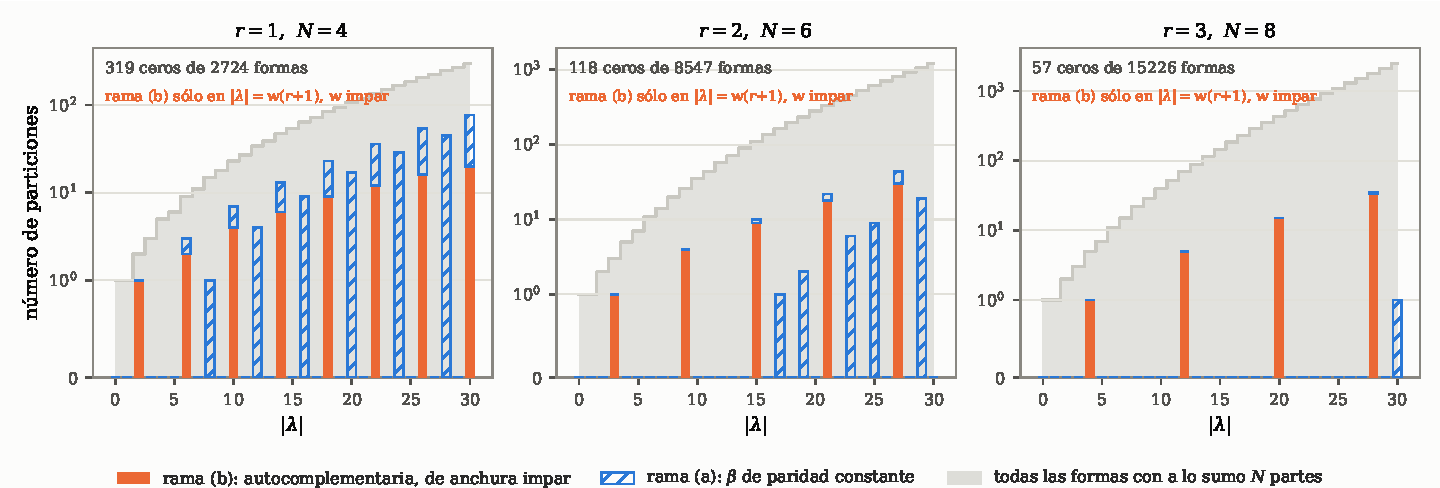
\includegraphics[width=\textwidth]{fig_zeros_es.pdf}
\caption{El lugar de anulación del Teorema \ref{thm:zeros}, contado en lugar de dibujado. Para cada
tamaño $|\lambda|$ las barras dan el número de particiones con a lo sumo $N$ partes que se anulan,
separadas por rama; el escalón sombreado es el número total de formas de ese tamaño, en el mismo eje,
de modo que la rareza del lugar se ve y no se afirma. Los tamaños que llevan la rama (b) son
exactamente los múltiplos $w(r+1)$ con $w$ impar, por el Corolario \ref{cor:sizes}; la rama (a) ocupa
otros tamaños y necesita que el conjunto beta se salte una paridad por completo, razón por la cual
está ausente en $|\lambda|$ pequeño en cuanto $N$ crece.}
\label{fig:zeros}
\end{figure} Conviene dejar constancia de que el enunciado
análogo para todo el lugar de anulación es falso: la rama (a) no está confinada a esa progresión, y
por eso la condición hay que leerla de la rama (b) sola.

\begin{theorem}[un par]\label{thm:r1}
Para $r=1$ vale también el recíproco: $\Psi_1(\lambda)=0$ solo si se cumple {\rm(a)} o {\rm(b)}.
\end{theorem}

\begin{theorem}[dentro del rango de Littlewood]\label{thm:stable}
Para todo $r$ y toda $\lambda$ con $\ell(\lambda)\le N/2$ vale el recíproco. Equivalentemente, en ese
rango $\Psi_r(\lambda)=0$ si y solo si $\lambda=(k^{\,N/2})$ con $k$ impar.
\end{theorem}

\begin{remark}[los rectángulos son donde se detienen los argumentos generales]
Vale la pena advertir que los dos sitios donde falla un argumento general de este artículo son
rectángulos, a dos alturas distintas y por dos razones distintas. A altura $N/2$ un rectángulo impar
es autocomplementario de anchura impar, luego se anula; por el Teorema \ref{thm:stable} son las
únicas formas del rango de Littlewood que lo hacen, y en la demostración son precisamente aquellas
para las que no se puede construir el testigo asociado. A altura completa el objeto no se anula, sino
que degenera en sentido contrario: $s_{(c^{\,N})}(x)=(x_1\cdots x_N)^{c}$ es un monomio, de modo que
sobre cualquier alfabeto $A$ el valor es $\det(A)^{c}$ y de la forma no sobrevive nada ---que con
$t=2$ es el caso {\rm(i)} de la Proposición \ref{prop:rect}, el único allí en el que la paridad de
$c$ no interviene---. Entre ambas alturas el argumento genérico se aplica sin cambios. Los
rectángulos no son una molestia que haya que tratar caso por caso: son el borde de la forma, y cada
uno de los dos extremos rompe una hipótesis distinta ---el primero la existencia de un testigo, el
segundo la no degeneración del triple de intervalos---.
\end{remark}

\begin{theorem}[el criterio en general]\label{conj:crit}
Para todo $r$ y toda $\lambda\in\PP_N$, $\Psi_r(\lambda)=0$ si y solo si se cumple {\rm(a)} o
{\rm(b)}.
\end{theorem}

\noindent Demostrado al final de la \S\ref{sec:zeros}, módulo el Teorema \ref{thm:PvW}.

Los Teoremas \ref{thm:zeros}--\ref{thm:stable} se demuestran en las
\S\S\ref{sec:brancha}--\ref{sec:conv}, y el Teorema \ref{conj:crit} --- el criterio para todo
$r$ --- al final de esta sección, por una vía independiente de los tres. Lo enunciamos aparte por dos
razones. Es el único resultado del artículo que se apoya en algo ajeno, el Teorema
\ref{thm:PvW}; y las dos vías que llevan a él no son la misma vía. La de Littlewood lo reduce, en la
\S\ref{sec:unstable}, a un único enunciado de existencia, y esa reducción no se completa: el rango
$\ell(\lambda)>N/2$ es exactamente donde la regla de restricción deja de aplicarse y, aunque el
Lema \ref{lem:AtoSp} resuelve allí los valores, el enunciado sobre los coeficientes no --- el
certificado que propusimos para él falla, por la Proposición \ref{conj:iso}. El argumento extremal
de las \S\S\ref{sec:extremal} y \ref{sec:rigidity} no entra en ese rango en absoluto: trabaja en
la filtración por grados del numerador y no se cruza jamás con un coeficiente de Littlewood.

Leído sobre el grupo y no sobre el alfabeto, el mismo teorema describe una propiedad de rigidez, y lo
enunciamos aparte porque es la forma en que lo querría alguien de teoría de representaciones. La
traducción no es nuestra ni es nueva: que una representación de $O(N)$ sea estable por $\det$
exactamente cuando su carácter se anula fuera de la componente identidad es elemental, y que eso sea
la condición $m_\nu=m_{\nu^{*}}$ sobre los asociados de Littlewood \cite{Lit50} es clásico. El
corolario reclama por tanto exactamente lo que reclama el Teorema \ref{conj:crit}, y nada más.

\begin{corollary}[rigidez frente al giro por el determinante]\label{cor:dettwist}
Sean $N=2r+2$ y $\lambda\in\PP_N$, y sea $V_\lambda$ el $GL(N)$-módulo polinómico irreducible de peso
máximo $\lambda$. Entonces
\[
V_\lambda\big|_{O(N)}\;\cong\;V_\lambda\big|_{O(N)}\otimes\det
\]
si y solo si $\beta(\lambda)$ tiene paridad constante, o $\lambda$ es autocomplementaria de anchura
impar. Equivalentemente: \eqref{eq:branches} clasifica exactamente los $GL(N)$-módulos polinómicos
irreducibles cuya restricción a $O(N)$ es estable por el carácter del grupo de componentes.
\end{corollary}

\begin{proof}
En característica $0$ un $O(N)$-módulo de dimensión finita es semisimple y queda determinado por su
carácter, así que para $W=V_\lambda|_{O(N)}$ se tiene $W\cong W\otimes\det$ si y solo si
$\chi_W=\chi_{W\otimes\det}$. Esos dos caracteres coinciden automáticamente en la componente
identidad, y en la otra $\chi_{W\otimes\det}=-\chi_W$; luego la condición es que $\chi_W$ se anule en
$O(N)^{-}$. Todo elemento \emph{semisimple} de $O(N)^{-}$ es conjugado a uno de espectro
$(1,-1,z_1^{\pm1},\dots,z_r^{\pm1})$, que es el alfabeto de \eqref{eq:psir}; y como los semisimples
son densos en $O(N)^{-}$ y $\chi_W$ es regular, anularse en ese toro es anularse en toda la
componente. La condición es por tanto $\Psi_r(\lambda)\equiv0$, y el Teorema \ref{conj:crit} es el
criterio. El diccionario entre las dos lecturas es la expansión por asociados de Littlewood, recordada
en la \S\ref{sec:conv}.
\end{proof}

\noindent El crédito se reparte exactamente igual que en el Teorema \ref{conj:crit}, y conviene
repetirlo aquí porque el lenguaje de grupos puede hacer que un enunciado conocido parezca nuevo. Que
las dos familias \eqref{eq:branches} \emph{sean} estables por $\det$ no es nuestro: en el extremo de
la familia, la primera es de Karmakar \cite[Teorema 4.1(A)]{Kar24}, y la segunda es la complementación
sobre la familia de índices de Ayyer y Behrend \cite{AB19}, como recoge \eqref{eq:compl}. Lo que el
Teorema \ref{conj:crit} añade, y es todo lo que añade, es que no hay ninguna más.

\begin{remark}[lo que el núcleo ve, y lo que no]\label{rem:core}
La rama (a) es una condición sobre el núcleo, y sencilla: con un número $N$ fijo de números beta, el
perfil de residuos determina $\core_t(\lambda)$ ---es la coordenada de Garvan--Kim--Stanton
\cite{GKS90}---, de modo que toda condición sobre el perfil lo es sobre el núcleo. No es, sin
embargo, la anulación del núcleo sino su extremo opuesto: en $t=2$ la rama (a) dice
\[
\core_2(\lambda)=(N-1,N-2,\dots,1)\qquad\text{o}\qquad\core_2(\lambda)=(N,N-1,\dots,1),
\]
los dos $2$-núcleos más grandes que admiten $N$ números beta, mientras que
$\core_2(\lambda)=\varnothing$ es el perfil equilibrado. La rama (b) no mueve ni el perfil ni el
núcleo, y por tanto le es invisible. En consecuencia $\core_2$ \emph{no} determina si $\Psi_r$ se
anula, y el testigo más pequeño es el propio núcleo vacío: entre las formas con
$\core_2(\lambda)=\varnothing$ en $r=1$,
\[
(1,1),\ (3,3),\ (2,2,1,1),\ \dots\quad\text{se anulan, y}\quad
\varnothing,\ (2),\ (1^4),\ \dots\quad\text{no,}
\]
y el mismo corte ocurre en $r=2$ y $r=3$, allí también en las clases de núcleo $(1)$, $(2,1)$ y
$(3,2,1)$: sobre los rangos de la \S\ref{sec:verif} hay cinco clases de núcleo que llevan ambos
comportamientos, y el perfil determina el núcleo sin ninguna colisión sobre $260$ perfiles con
$t\le5$. No puede existir, pues, ninguna reformulación del Teorema \ref{thm:zeros} en términos de
$\core_2(\lambda)$: el criterio necesita la forma y no solo su núcleo. Leídos contra el Teorema
\ref{thm:LR}, donde el núcleo vacío es exactamente lo que decide, los dos criterios discrepan en
ambas direcciones ---$(1,1)$ tiene $2$-núcleo vacío y $\Psi_1=0$, mientras que $(1)$ tiene
$2$-núcleo no vacío y $\Psi_1\ne0$.
\end{remark}

La familia de índices de (b) no es nueva: es precisamente la que Ayyer y Behrend destacan
\cite[observación tras el Teo.~3]{AB19}, junto con la obstrucción de paridad que registran allí ---una
partición no puede ser autocomplementaria en un rectángulo $a\times b$ con $a$ y $b$ ambos impares, y
aquí $a=N$ es par, luego el caso admisible es $b=w$ impar. Lo que sus teoremas dicen de esas formas es
que el carácter \emph{factoriza}; allí el alfabeto lleva el punto fijo $+1$ y tiene determinante $+1$.
El nuestro lleva $+1$ y $-1$, y tiene determinante $-1$.

\keybox{Sobre la \emph{misma} familia de formas, el alfabeto de determinante $+1$ hace que el
carácter factorice y el de determinante $-1$ hace que se anule. Una letra separa una factorización de
una aniquilación, y quien decide es el determinante del alfabeto; la identidad \eqref{eq:compl} de
más abajo es donde ocurre la separación.}


\subsection{Rama (a): el alfabeto al cuadrado}\label{sec:brancha}

Esta rama es de Karmakar, en el extremo. \cite[Teorema 4.1(A)]{Kar24} evalúa un carácter de
$\mathrm{GL}(n,\CC)$ en $C_{n-k,k}=(1,\dots,1,-1,\dots,-1)$ y da
$\chi_\lambda(C_{n-k,k})=0$ cuando $\#\eta_0(\lambda)>n-k$, donde su
$\eta_i(\lambda)=\{a\in\lambda+\rho: a\equiv i \bmod 2\}$ es exactamente la partición de
$\beta(\lambda)$ en $E$ y $O$ que usamos aquí; en $k=1$, tras su normalización por el carácter
determinante, eso es la rama (a). El argumento de una línea que sigue se incluye porque es el que
reutiliza el resto de la sección, no porque sea nuevo.

\begin{proof}[Demostración del Teorema \ref{thm:zeros}, rama {\rm(a)}]
Sea $A=\{1,-1,z_1,\bar z_1,\dots\}$. Si $\beta=2\gamma$, entonces
$\det(a^{\beta_j})_{a\in A}=\det\big((a^2)^{\gamma_j}\big)_{a\in A}$, y si $\beta=2\gamma+1$ ocurre lo
mismo tras extraer $\prod_{a\in A}a$. En ambos casos el bialternante factoriza a través del alfabeto
al cuadrado $A^2=\{1,1,z_1^{2},\bar z_1^{2},\dots\}$, en el que la letra $1$ aparece dos veces porque
$1^2=(-1)^2$. Hay dos filas iguales.
\end{proof}

\subsection{Rama (b): una torsión por el determinante, y autodualidad}

\begin{proof}[Demostración del Teorema \ref{thm:zeros}, rama {\rm(b)}]
Sea $\hat\lambda$ el complementario de $\lambda$ en la caja $w\times N$, leído del revés. En
conjuntos beta, $\beta(\hat\lambda)=c-\beta(\lambda)$ recorrido en sentido inverso, con $c=w+N-1$, y
$\hat\lambda$ es el peso máximo de $V_\lambda^{*}\otimes\det^{\,w}$ como $\mathrm{GL}(N)$-módulo. Si
$\lambda=\hat\lambda$, entonces $V_\lambda\cong V_\lambda^{*}\otimes\det^{\,w}$. Restrinjamos a
$O(N)$: toda representación de $O(N)$ es autodual, luego
$V_\lambda|_{O(N)}\cong V_\lambda^{*}|_{O(N)}\cong V_\lambda|_{O(N)}$, de donde
\[
V_\lambda|_{O(N)}\;\cong\;V_\lambda|_{O(N)}\otimes\det^{\,w}.
\]
El alfabeto \eqref{eq:psir} es un elemento del toro de la componente $\det=-1$, así que para $w$
impar la torsión es por $\det$ mismo y el carácter se anula ahí. Para $w$ par, $\det^{\,w}$ es
trivial y el argumento no da nada: por eso la paridad de $w$ no es un adorno.
\end{proof}

Equivalentemente, y esto es el cálculo en lugar de la representación, la identidad de complementación
estándar da
\begin{equation}\label{eq:compl}
s_{\hat\lambda}(A)\;=\;\Big(\textstyle\prod_{a\in A}a\Big)^{c}\,(-1)^{\binom{N}{2}}(-1)^{r}\,
s_\lambda(A)\;=\;(-1)^{c}\,(-1)\,s_\lambda(A),
\end{equation}
usando que $A$ es cerrado por inversión ---$A^{-1}$ es $A$ con los $r$ pares recíprocos
transpuestos, lo que aporta $(-1)^r$--- y que $\prod_{a\in A}a=-1$. Con $c$ par esto se lee
$s_{\hat\lambda}=-s_\lambda$, y una forma autocomplementaria queda aniquilada. La rama (b) del
Teorema \ref{thm:zeros} es por tanto un corolario de dos líneas de una identidad de manual sobre una
familia de índices conocida, y no la reclamamos como nada más. La Figura \ref{fig:involution} dibuja
el emparejamiento que hace la identidad, y a su lado la misma forma con una caja movida, donde el
emparejamiento se rompe; el contenido de la sección es el recíproco.

\subsection{El recíproco}\label{sec:conv}

\begin{figure}[t]
\centering
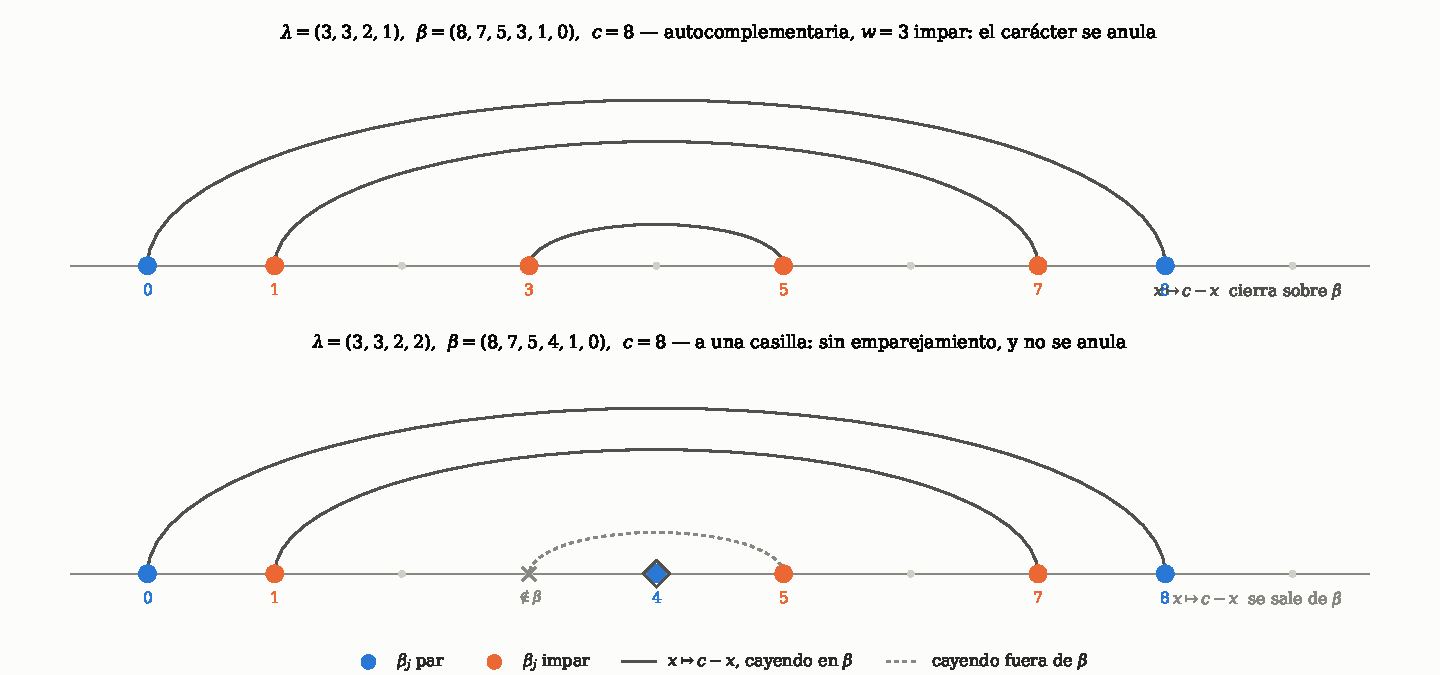
\includegraphics[width=\textwidth]{fig_involution_es.pdf}
\caption{Por qué la autocomplementariedad mata el carácter. Al desarrollar por las dos filas
congeladas quedan términos indexados por pares $(e,o)$ con $e\in E$, $o\in O$, y la reflexión
$x\mapsto c-x$ actúa sobre ellos. Arriba, una forma autocomplementaria de anchura impar: todo arco
cae dentro de $\beta$ y une entradas de igual paridad, porque $c$ es par. Abajo, la misma forma con
una caja movida: el arco $5\mapsto3$ se sale de $\beta$, así que no hay emparejamiento y nada se
cancela. El rombo marca el punto fijo de la reflexión, que no puede darse dentro de un par de
paridades opuestas ---y ésa es la razón de que la involución sea libre.}
\label{fig:involution}
\end{figure}

\begin{proof}[Demostración del Teorema \ref{thm:r1}]
Pongamos $c_\ast=z+\bar z$ y definamos $S_n$ por $S_0=0$, $S_1=1$, $S_{n+1}=c_\ast S_n-S_{n-1}$, de
modo que $\deg_{c_\ast}S_n=n-1$ y $S_{-n}=-S_n$; el valor $S_{-1}=-1$ se usa siempre que
$\beta_N=0$. Como $\Phi_A=(x^2-1)(x^2-c_\ast x+1)$, un polinomio $P$ soportado en $\beta$ es
divisible por $\Phi_A$ exactamente cuando $P(1)=P(-1)=0$ y $P\equiv0$ módulo $x^2-c_\ast x+1$.
Separando $P(\pm1)$ por paridad y reduciendo $x^n\equiv S_nx-S_{n-1}$, la admisibilidad se convierte
en la singularidad de la matriz $4\times4$ con filas $[\beta_j\ \mathrm{par}]$,
$[\beta_j\ \mathrm{impar}]$, $S_{\beta_j}$, $S_{\beta_j-1}$. Desarrollando por las dos filas de
paridad y usando la identidad de d'Ocagne \cite{Doc} para esta recurrencia,
\begin{equation}\label{eq:docagne}
S_bS_{b'-1}-S_{b'}S_{b-1}=-S_{b-b'},
\end{equation}
cada bloque $2\times2$ colapsa a un \emph{único} $S$, indexado por la diferencia de los dos $\beta$
supervivientes. Los $S_n$ distintos tienen grados distintos en $c_\ast$ y son por tanto linealmente
independientes, de modo que la suma con signo se anula solo mediante un emparejamiento exacto de
índices iguales con signos opuestos. El análisis de casos es finito: $|E|\in\{0,4\}$ es la rama (a);
$|E|\in\{1,3\}$ deja tres términos cuyos índices son las tres diferencias dos a dos de un conjunto de
tres elementos y por tanto siempre distintas, así que no existe emparejamiento y el valor no es nulo;
y para $|E|=2$ hay cuatro términos y tres emparejamientos perfectos, y se comprueban los seis
patrones de paridad directamente. Para $E=\{\beta_1,\beta_4\}$ y para $E=\{\beta_2,\beta_3\}$ solo
uno de los tres emparejamientos está disponible, e impone la única condición
$\beta_1+\beta_4=\beta_2+\beta_3$, que es la rama (b); para los cuatro patrones restantes, cada uno
de los tres emparejamientos obliga a dos entradas distintas de $\beta$ a coincidir, así que ninguno
está disponible y el valor no es nulo.
\end{proof}

La identidad \eqref{eq:docagne} es clásica. El colapso que produce es un accidente de rango uno: dos
letras admiten un solo hueco, luego $s_{(m,n)}(z,\bar z)=S_{m-n+1}$ depende solo de ese hueco. No hay
análogo de rango $r$. Lo habría si existiera una forma cerrada de $s_\mu$ en alfabeto recíproco para
\emph{toda} $\mu$; \cite{CK09} la dan para formas rectangulares y \cite{AB19} para las
autocomplementarias, y nadie en general.

Para $r$ general usamos asociados, en el sentido de Littlewood \cite{Lit50}.
En el coset $\det=-1$, la relación $[\nu^{*}]=[\nu]\otimes\det$ da
$\Psi_r=\sum_\nu\big(m_\nu-m_{\nu^{*}}\big)\chi_{[\nu]}$, luego $\Psi_r=0$ si y solo si
$m_\nu(\lambda)=m_{\nu^{*}}(\lambda)$ para toda $\nu$; equivalentemente, si y solo si
$V_\lambda|_{O(N)}$ es invariante por $\det$. Esa equivalencia es el diccionario a través del cual se
lee el Corolario \ref{cor:dettwist}, y es lo que convierte el criterio en un enunciado sobre módulos
y no sobre un alfabeto. Un testigo es por tanto una sola $\nu$ con
$m_\nu\ne m_{\nu^{*}}$, y se puede construir.

El \cite[Teorema 4.1]{Kar24} de Karmakar determina el valor en el extremo $z_i=1$, que es un elemento
de orden dos: el caso (A) es la rama (a), el caso (B) es una dimensión no nula, y el caso (C) deja una
suma alternante de productos de dimensiones sin criterio de anulación asociado. La rama (b) vive en
ese caso (C), de modo que el teorema siguiente no es consecuencia suya. Y el caso (B) tampoco ayuda
más al crecer $r$: con $k=1$ pide que $N-1$ de los $N$ números beta compartan paridad, y la forma más
pequeña que lo hace es la escalera $(2r-1,2r-2,\dots,1)$, de tamaño $r(2r-1)$, así que sobre un rango
fijo de $|\lambda|$ su caso de no anulación sólo se ve para $r$ pequeño --- su resultado es más
afilado exactamente donde el nuestro es más fácil. Lo que conecta el extremo con
la curva es la rigidez, y la rigidez es un enunciado sobre nuestro objeto y no sobre el elemento de
orden dos: sobre los rangos de la \S\ref{sec:verif} se cumple en $\ell(\lambda)\le N/2$ sin excepción
y falla fuera, que es la Observación \ref{rem:rankone}.

\begin{proof}[Demostración del Teorema \ref{thm:stable}]
La rama (a) no puede darse: con $\ell(\lambda)\le N/2$ se anulan al menos dos partes finales, luego
$\beta$ contiene dos enteros consecutivos. En el rango de Littlewood,
$m_\nu(\lambda)=\sum_{\beta'\ \mathrm{par}}c^{\lambda}_{\nu\beta'}$, y el término
$\beta'=\emptyset$ da $m_\mu\ge1$ para toda $\mu\subseteq\lambda$. Tomemos $\mu$ así. Si
$\ell(\lambda)<N/2$, tomamos $\mu=\lambda$: entonces
$\ell(\lambda^{*})=N-\ell(\lambda)>\ell(\lambda)$, luego $\lambda^{*}\not\subseteq\lambda$ y
$m_{\lambda^{*}}=0\ne m_\lambda$. Si $\ell(\lambda)=N/2$ y $\lambda_{N/2}$ es par, tomamos
$\mu=(\lambda_1,\dots,\lambda_{N/2-1})$; entonces $\beta'=(\lambda_{N/2})$ es par, $\lambda/\mu$ es
una tira horizontal y $m_\mu\ge1$ con $\ell(\mu)<N/2$, así que se aplica a $\mu$ el cálculo anterior.
Si $\ell(\lambda)=N/2$ y $\lambda$ no es un rectángulo, sea $j\le N/2-1$ el mayor índice con
$\lambda_j>\lambda_{j+1}$ y quitemos la última fila y además una caja de la fila $j$; entonces
$\beta'=(\lambda_{N/2}+1)$ es par y $\lambda_j\ge\lambda_{N/2}+1$ mantiene $\lambda/\mu$ como tira
horizontal. Un rectángulo par $\lambda=(k^{\,N/2})$ ya lo cubre la segunda construcción, de modo que
el único caso que queda es $k$ impar, donde no está disponible ninguna de las dos construcciones
---y eso es la rama {\rm(b)}---.
\end{proof}

\subsection{Fuera del rango de Littlewood}\label{sec:unstable}

Para $\ell(\lambda)>N/2$ la regla de restricción adquiere etiquetas no estándar, y las reglas de
modificación que las reducen son las de King \cite{King71}; Koike y Terada
\cite{KT87} registran que la especialización de tipo $D$ manda un carácter universal a
$0$ o a $\pm$ otro, y Fauser, Jarvis, King y Wybourne observan que más allá de los dos casos clásicos
\emph{``la teoría general, con infinitos casos, requiere un formalismo aún no disponible''}
\cite[\S4]{FJKW05}. Extensiones de la regla de Littlewood a todos los parámetros sí existen para los
dos casos clásicos --- las reglas de modificación de Newell \cite{New51}, Sundaram \cite{Sun90} en el
caso simpléctico, la demostración de Gavarini por álgebras de Brauer \cite{Gav99}, y Enright y
Willenbring \cite{EW04}, cuyo Teorema 4 da la multiplicidad como una suma alternante sobre el grupo de
Weyl que en casos favorables colapsa a una diferencia de dos coeficientes de Littlewood
\cite[\S7.11]{EW04}. Esa observación de \cite{FJKW05} es de 2005, y conviene dejar escrito que el
hueco que señala se ha llenado desde entonces por el lado que necesitamos: Frohmader
\cite{Frohmader} da reglas de ramificación combinatorias para $GL_n\downarrow O_n$ y
$GL_{2n}\downarrow Sp_{2n}$ que generalizan las reglas de restricción de Littlewood y son, en sus
palabras, \emph{«válidas para todos los parámetros, es decir, no hay restricciones de rango
estable»}; la multiplicidad pasa a ser una suma de coeficientes de Littlewood--Richardson
generalizados $c^{\lambda}_{\mu\nu}(O_n)$ leídos de condiciones de bandera sobre tablas de
Littlewood--Richardson ordinarias, sin ninguna regla de modificación. No la usamos abajo, y decimos
por qué en un momento; pero es el instrumento natural para la única pregunta que esta sección deja
abierta, y volvemos a ella en el Problema \ref{prob:instrument}.

La ruta de aquí es la dual: mantener universales los coeficientes, que lo son en
todo rango, y trasladar toda la dependencia del rango a los valores, donde un solo lema la liquida.
Sobre este alfabeto no hace falta formalismo alguno para las etiquetas, y la razón es que los valores
no son valores de tipo $D$.

Añadir una letra $c$ a un alfabeto actúa sobre el anillo de funciones simétricas por
$p_k\mapsto p_k+c^k$; escribimos $\iota_c$ para ese homomorfismo. De la función generatriz de las
funciones simétricas homogéneas completas, $h_m(W,c)-c\,h_{m-1}(W,c)=h_m(W)$ para todo $m$.

\begin{lemma}[el alfabeto es simpléctico]\label{lem:AtoSp}
$\iota_{-1}\iota_{1}\,o_\nu=sp_\nu$ para toda partición $\nu$, como identidad entre caracteres
\emph{universales} de Koike--Terada en $\Lambda$. En particular, para el alfabeto
\eqref{eq:psir},
\begin{equation}\label{eq:AtoSp}
o_\nu(A)\;=\;sp_\nu(z_1,\dots,z_r)
\end{equation}
sin hipótesis sobre $\ell(\nu)$ y sin signo. Para $\ell(\nu)>r$ el miembro derecho es ese
carácter universal especializado a $r$ variables, no un carácter irreducible de $Sp(2r)$; son las
reglas de modificación de más abajo las que lo pliegan sobre uno.
\end{lemma}

\begin{proof}
Ambos pasos son de Ayyer y Kumari, y ambos son la misma manipulación: la recurrencia convierte las
operaciones de columna $C_j\to C_j-c\,C_{j-1}$, aplicadas para $j=n,\dots,2$ en ese orden, en un
cambio de tipo de carácter, y operaciones de esa forma dejan invariante un determinante. Con $c=1$
llevan el determinante que define $o_\nu$, evaluado en $(W,1)$, al del carácter universal ortogonal
impar $so_\nu$ sobre $W$, que es el diccionario de Koike y Terada en la forma
$so_\nu(X)=o_\nu(X,\bar X,1,0,0,\dots)$ \cite[(2.13)]{AK25}. Con $c=-1$, donde la recurrencia es
\cite[Proposición 2.1]{AK25} y las operaciones se leen $C_j\to C_j+C_{j-1}$, llevan $so_\nu$ a
$sp_\nu$, que es \cite[Lema 3.2]{AK25}. Componiendo se obtiene el primer enunciado, y evaluándolo en
el alfabeto recíproco $(z_1,\dots,z_r)$ se obtiene \eqref{eq:AtoSp}.
\end{proof}

\noindent Como $\nu'_1=\ell(\nu)$, la tricotomía sobre $\nu'_1$ frente a $N/2=r+1$ es una tricotomía
sobre la longitud de $\nu$ frente al rango de $Sp(2r)$, y los tres hechos que necesitamos son
entonces las reglas de modificación simplécticas clásicas --- uno de los dos casos que
\cite{FJKW05} exceptúa --- leídas a través de \eqref{eq:AtoSp}: $o_\nu(A)=0$ cuando $\ell(\nu)=r+1$,
la anulación de un carácter simpléctico una fila más allá de su rango; $o_\nu(A)=\pm o_{\nu^{*}}(A)$
cuando $\ell(\nu)>r+1$, la regla de King plegando la etiqueta sobre una dominante; y lo mismo para
$\nu$ no estándar, que por el Lema \ref{lem:nonstd} son exactamente las altas. La expansión
$s_\lambda=\sum_\nu c_\nu o_\nu$, con $c_\nu=\sum_{\beta'\ \mathrm{par}}c^{\lambda}_{\nu\beta'}$, es
una identidad de funciones simétricas y vale en todo rango; especializarla en \eqref{eq:psir} deja
por tanto todo término sobre $\{o_\mu(A):\ell(\mu)\le r\}$, que por \eqref{eq:AtoSp} es el conjunto de
los caracteres irreducibles de $Sp(2r)$ y es por ello linealmente independiente. La Figura
\ref{fig:reduction} clasifica las etiquetas en las cuatro clases que describe este párrafo y calcula
$o_\nu(A)$ en cada una, de modo que puede verse que la reducción aterriza donde se afirma. Luego

\begin{figure}[!ht]
\centering
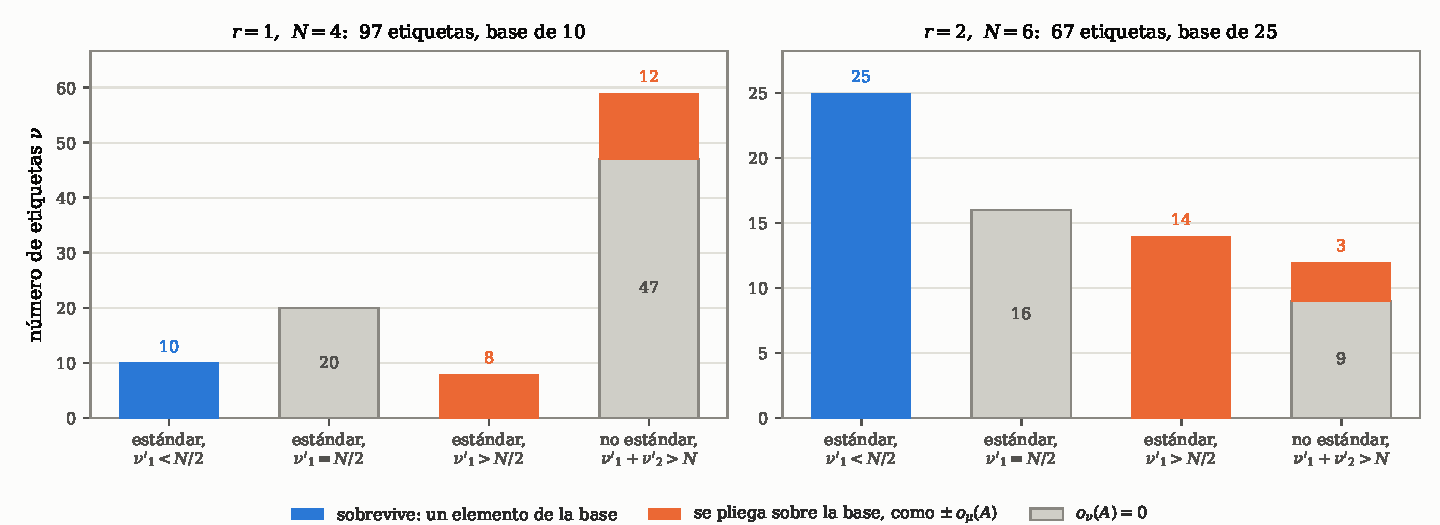
\includegraphics[width=\textwidth]{fig_reduction_es.pdf}
\caption{La reducción del Lema \ref{lem:AtoSp}, dibujada. Cada etiqueta
$\nu$ que aparece en $s_\lambda=\sum_\nu c_\nu o_\nu$ se coloca en una de cuatro clases y se calcula
su valor $o_\nu(A)$. Las etiquetas autoasociadas se anulan, todas ellas; las estándar con
$\nu'_1>N/2$ se pliegan sobre la base como $\pm o_{\mu}(A)$; las no estándar o se anulan o se pliegan
sobre un único elemento de la base con coeficiente $\pm1$. Por \eqref{eq:AtoSp} estas tres son las
reglas de modificación simplécticas disfrazadas, con las clases cortadas por $\ell(\nu)$ frente al
rango $r$; la figura se calculó antes de advertirlo y se deja tal cual. Todo aterriza en la base
independiente $\{o_\mu(A):\ell(\mu)\le r\}$, que es lo que convierte la anulación en la condición
finita \eqref{eq:Cmu}. Las alturas de las barras son recuentos de etiquetas sobre el rango en que se
calculó cada panel, menor que el de la fila correspondiente de la \S\ref{sec:verif}; lo que la imagen
cuenta es la clasificación, no el recuento.}
\label{fig:reduction}
\end{figure}
\begin{equation}\label{eq:Cmu}
\Psi_r(\lambda)=\sum_{\ell(\mu)\le r}C_\mu(\lambda)\,o_\mu(A),
\qquad
\Psi_r(\lambda)=0\iff C_\mu(\lambda)=0\ \text{para toda }\mu,
\end{equation}
donde $C_\mu=c_\mu\pm c_{\mu^{*}}+\sum\pm c_\nu$, sumando sobre las $\nu$ no estándar que se reducen
a $\mu$. La reducción se hace en dos pasos y no en uno: la mayoría de las etiquetas no estándar se
emparejan con una asociada dentro del rango, mientras que $21$ de ellas --- $18$ con $r=1$ y $3$ con
$r=2$ --- no tienen asociada en rango y se reducen aparte, cayendo cada una en el span de los valores
estándar con coeficientes enteros.

Habíamos calculado los tres hechos antes de localizarlos, y dejamos constancia del cálculo porque es
lo que dibuja la figura de abajo: \texttt{sec8\_derivation.sage} comprueba \eqref{eq:AtoSp}
directamente para todo $|\nu|\le8$, confirma que las etiquetas de longitud $r+1$ se anulan y que las
más largas se pliegan sobre la base con un signo, y verifica la independencia como un cálculo de
rango, con $r=1,2,3$. Un control que tenía que dispararse: $\iota_1 o_\nu$ y $\iota_{-1}o_\nu$
coinciden con $sp_\nu$ sólo para $\nu=\varnothing$, de modo que hacen falta las dos letras y
\eqref{eq:AtoSp} es un enunciado sobre el par recíproco y no sobre ninguna de las dos por separado.
\texttt{sec8\_formulas.sage} comprueba la demostración y no el enunciado --- la recurrencia con cuatro
valores de $c$, los dos determinantes que definen los caracteres frente a una implementación
independiente, y las operaciones de columna entrada por entrada. Esta última comprobación se ganó el
sueldo: un borrador previo de la demostración escribía $C_j\to C_j+C_{j-1}$ con $c=1$, que es el signo
que \cite[Lema 3.2]{AK25} usa para su propio paso con $c=-1$.

Las etiquetas no estándar, que son aquí toda la obstrucción, no pueden ser pequeñas:

\begin{lemma}[las etiquetas no estándar son grandes]\label{lem:nonstd}
Toda $\nu$ no estándar que aparezca en el desarrollo cumple $|\nu|\ge N+1=2r+3$. En consecuencia, si
$|\lambda|\le2r+2$ ninguna etiqueta no estándar está contenida en $\lambda$, la última suma de $C_\mu$
queda vacía y $C_\mu(\lambda)=c_\mu(\lambda)\pm c_{\mu^{*}}(\lambda)$ --- sin hipótesis alguna sobre
$\ell(\lambda)$, luego también fuera del rango de Littlewood.
\end{lemma}

\begin{proof}
Como $c^{\lambda}_{\nu\beta'}=0$ salvo si $\nu\subseteq\lambda$, solo aparecen etiquetas con
$\ell(\nu)\le\ell(\lambda)\le N$. Ser no estándar significa $\nu'_1+\nu'_2>N$. Si $\nu$ tuviera una
sola columna sería $\nu'_2=0$ y haría falta $\nu'_1=\ell(\nu)>N$, que queda excluido; luego
$\nu'_2\ge1$ y $|\nu|\ge\nu'_1+\nu'_2>N=2r+2$. Así que una $\nu$ no estándar solo puede contribuir
cuando $|\lambda|\ge|\nu|\ge2r+3$.
\end{proof}

\noindent Como $\ell(\lambda)>N/2$ obliga a $|\lambda|\ge r+2$, el Lema \ref{lem:nonstd} resuelve de
golpe la franja $r+2\le|\lambda|\le2r+2$ del rango inestable: ahí la regla de Littlewood se aplica
literalmente y el recíproco se sigue por el argumento del Teorema \ref{thm:stable}. Lo que esta ruta
todavía tiene que cruzar es $|\lambda|>2r+2$.


Dos hechos exactos acotan a los competidores. Primero, $\ell(\mu^{*})=N-\ell(\mu)$, de modo que
$\ell(\mu)\le N-1-\ell(\lambda)$ obliga a $\mu^{*}\not\subseteq\lambda$ y a $c_{\mu^{*}}=0$. Segundo,
una $\nu$ no estándar cumple $\nu'_1+\nu'_2>N$ con $\nu'_2\le\nu'_1$, luego $2\ell(\nu)>N$ y
$\ell(\nu)\ge r+2$; en particular, en el rango de Littlewood ninguna etiqueta no estándar cabe dentro
de $\lambda$. Llamemos $\mu$ \emph{aislante} para $\lambda$ si exactamente una de las etiquetas que
alimentan $C_\mu$ está contenida en $\lambda$; entonces $C_\mu=\pm c_\nu\ne0$ y
$\Psi_r(\lambda)\ne0$. Lo que la ruta pide ahí es un único enunciado de existencia ---abierto como
enunciado de existencia, aunque no como teorema, pues el Teorema \ref{conj:crit} no pasa por él---.

\begin{proposition}[el testigo aislante no siempre existe]\label{conj:iso}
En $r=2$ la forma $\lambda=(5,5,2,1)$ cumple $\Psi_2(\lambda)\ne0$ y no es de tipo {\rm(a)} ni de
tipo {\rm(b)}, y ninguna $\mu$ es aislante para ella: toda $\mu$ cuyo $C_\mu$ tenga un contribuyente
no nulo dentro de $\lambda$ tiene exactamente dos, a saber $\mu$ y su asociado $\mu^{*}$.
\end{proposition}

Habíamos propuesto el testigo aislante como la vía hacia el Teorema \ref{conj:crit}, y no llega. La
razón se lee en el lema de aislamiento: exige $\ell(\mu)\le N-1-\ell(\lambda)$, lo que con
$\ell(\lambda)=4$ y $N=6$ deja solo $\mu$ de una fila, y una forma tan ancha como $(5,5,2,1)$
contiene a todos los asociados. Sobre $r=2$ y $|\lambda|\le14$ hay once formas así, la menor esta
misma, y ninguna por debajo de $|\lambda|=13$, que es la razón de que el certificado parezca sólido
en rangos pequeños. El Teorema \ref{conj:crit} en sí queda intacto ---afirma que los $C_\mu$ se
anulan, no que exista un certificado--- pero esta vía hacia él queda cerrada. La que sí llega, la
\S\ref{sec:rigidity}, no pasa por el rango de Littlewood, y por eso el fallo de aquí cuesta la
explicación y no el teorema.

El mecanismo alcanza mucho: en $r=2$ y $|\lambda|\le14$, $227$ de las $238$ formas inestables no
nulas llevan un testigo aislante demostrado. Y alcanza más de lo que el hecho (ii) permite por sí
solo ---el mínimo real de $\ell(\nu)$ sobre las $\nu$ no estándar con $o_\nu(A)\ne0$ es allí $5$,
frente al $r+2=4$ que da la cota. Lo que lo derrota es la anchura y no la altura: la base de
\eqref{eq:Cmu} crece con $r$ y las etiquetas competidoras están obligadas a ser altas, así que
leíamos el aislamiento como algo que se facilita con $r$, y a lo largo del eje de la altura así es;
el residuo vive donde $\lambda$ es lo bastante ancha para tragarse los asociados. Esa lectura predice
dónde el residuo \emph{no} está: en $r=3$ el lema de aislamiento permite $\ell(\mu)\le7-\ell(\lambda)$,
de modo que una forma tiene que ser más ancha que en $r=2$ antes de poder tragarse todos los
asociados, y los mismos tamaños deberían salir limpios. Y salen ---sobre $r=3$ y $|\lambda|\le13$ las
$149$ formas inestables no nulas llevan todas un testigo demostrado y el residuo es vacío---, lo cual
es un control sobre la explicación, no un paso hacia el Teorema \ref{conj:crit}. En $r=1$ la
cuestión no se plantea, pues ese caso lo resuelve por separado el Teorema \ref{thm:r1}.

La herramienta a la que uno acude primero no encaja. La saturación, en la forma de panal de Knutson
y Tao \cite{KT99}, decide cuándo un coeficiente de Littlewood--Richardson aislado es positivo, y todo
competidor que alimenta a $C_\mu$ lo es en cuanto su etiqueta cabe dentro de $\lambda$. Lo que un
$\mu$ aislante pide no es positividad sino \emph{aislamiento}: que exactamente uno de ellos quepa. La
positividad es lo que vuelve difícil la pregunta, no lo que la responde, y no conocemos herramienta
alguna dirigida a la segunda.

\begin{figure}[t]
\centering
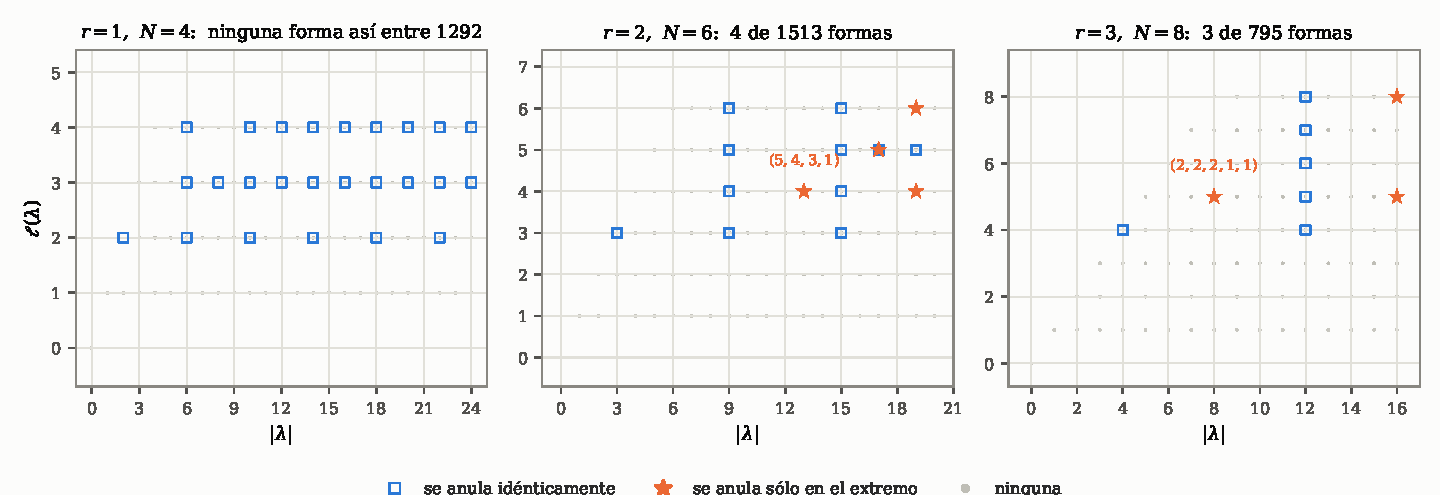
\includegraphics[width=\textwidth]{fig_phase_es.pdf}
\caption{Dónde deja de ser típico un solo par recíproco. Cada partición con a lo sumo $N$ partes es un
punto en $(|\lambda|,\ell(\lambda))$; la clase dibujada con estrella es la que se anula en el extremo
$z_i=1$ sin anularse idénticamente, y es todo el contenido de la imagen; cada panel nombra a su
miembro más pequeño y la Observación \ref{rem:rankone} enumera los demás.
Los paneles cubren $|\lambda|\le24$, $20$ y $16$ respectivamente. En $r=1$ la clase
está vacía sobre las $1292$ formas del rango, porque allí el objeto es $\pm$ un carácter genuino y su
valor en la identidad es una dimensión. A partir de $r=2$ aparecen ejemplos genuinamente virtuales y
la clase deja de estar vacía ---no que toda forma lo sea: el Cuadro \ref{tab:virtual} cuenta las dos
cosas---. Véase la Observación \ref{rem:rankone}.}
\label{fig:phase}
\end{figure}

\begin{remark}[el accidente de rango uno, y dónde se separan los dos rangos]\label{rem:rankone}
En $r=1$ el objeto es $\pm$ un carácter genuino, así que su valor en la identidad es una dimensión y
$\Psi_1(\lambda)\equiv0$ si y solo si $\Psi_1(\lambda)|_{z=1}=0$. En $r\ge2$ la expansión plegada
\emph{puede} ser genuinamente virtual ---no que lo sea siempre, y el Cuadro \ref{tab:virtual} cuenta
las dos columnas---, y basta una forma en que lo sea para romper esa equivalencia:
$\lambda=(5,4,3,1)$ con $r=2$ cumple
$\Psi_2(\lambda)\ne0$ y $\Psi_2(\lambda)|_{z_1=z_2=1}=0$. La Figura \ref{fig:virtual} muestra
los dos regímenes uno al lado del otro, sobre dos formas que difieren en una sola casilla. Sobre los rangos de la Figura
\ref{fig:phase}, la clase de tales formas está vacía en $r=1$ a lo largo de $1292$ particiones; en
$r=2$ consta de las cuatro formas $(5,4,3,1)$, $(5,5,4,2,1)$, $(10,5,3,1)$ y $(6,5,4,2,1,1)$, y en
$r=3$ de las tres formas $(2,2,2,1,1)$, $(5,5,4,1,1)$ y $(3,3,3,2,2,1,1,1)$; es delgada, pero no está
vacía, y un solo contraejemplo es todo lo que la equivalencia puede soportar. La implicación que sí
sobrevive ---anulación exacta $\Rightarrow$ anulación en el extremo--- es lo que hace del extremo un
tamiz válido y nada más. Por eso los resultados calculados en elementos de orden dos ---Karmakar
\cite{Kar24} a lo largo de toda esa familia, Eisenkölbl \cite{Eis07} en el equilibrado
$x_i=(-1)^i$--- hablan de un punto y no de la curva, y por eso el
Teorema \ref{thm:zeros} no es un corolario suyo para $r\ge2$.
\end{remark}

Conviene ponerle un número a lo que el tamiz del extremo deja escapar, porque el enunciado
cualitativo se lee con facilidad como una corrección pequeña. Sobre los rangos de la Figura
\ref{fig:phase}, el contraste $\Psi_r(\lambda)|_{z_i=1}=0$ señala $143$ formas en $r=1$, $22$ en $r=2$
y $9$ en $r=3$; de ellas, $0$, $4$ y $3$ respectivamente no se anulan idénticamente. El tamiz es
entonces exacto con un solo par, y la proporción de sus veredictos que resultan espurios crece con el
número de pares: $0\%$, $18\%$, $33\%$ sobre estos rangos. Un cálculo en el extremo es un filtro que
nunca se salta un cero genuino, y pasado un par no es nada más que eso. El caso de rango uno con
$t=2$, donde el tamiz resulta exacto porque el objeto es un carácter genuino, se trató aparte en
\cite{Mar26}; el alfabeto \eqref{eq:object} surgió allí, en un cálculo de líneas de Wilson sobre un
orbifold, y de ahí que el $-1$ aparezca como letra y no como elección.

Vale la pena separar la razón de que los dos rangos de $\ell(\lambda)$ se comporten de forma tan
distinta del mecanismo que lo demuestra. La regla de Littlewood dice qué etiquetas $\nu$ pueden
aparecer, y $\ell(\lambda)\le N/2$ es exactamente la condición bajo la cual las no estándar no caben
dentro de $\lambda$. El Lema \ref{lem:nonstd} dice que la obstrucción la gobierna $|\lambda|$ además
de $\ell(\lambda)$, así que la imagen honesta no es de dos rangos sino de una región: \emph{esta
ruta} alcanza el recíproco allí donde $\ell(\lambda)\le N/2$ o bien $|\lambda|\le2r+2$, y fuera de la
unión de ambas no llega ---el testigo aislante cubre casi todo lo que queda pero demostrablemente no
todo, por la Proposición \ref{conj:iso}---. El recíproco no está abierto ahí. El Teorema
\ref{conj:crit} lo resuelve para todo $r$ y toda $\lambda$ por el argumento extremal de las
\S\S\ref{sec:extremal}--\ref{sec:rigidity}, que no entra en este rango en absoluto. Lo que la región
marca es dónde deja de explicar la reducción de Littlewood, no dónde deja de valer el teorema.

%======================================================================
% ---- v2_new_subsections_es.tex ----
\subsection{El criterio en \texorpdfstring{$t=2$}{t=2}: el argumento extremal}\label{sec:extremal}

En esta subsección y en las dos siguientes, $t\ge2$ y $r\ge1$ son arbitrarios y
\[
  N:=t+2r,\qquad
  \Phi_{t,r}(\lambda;z):=s_\lambda\bigl(\zt,\,z_1,\zb_1,\dots,z_r,\zb_r\bigr),
\]
de modo que $\Phi_{t,1}$ es \eqref{eq:object} y $\Phi_{2,r}=\Psi_r$. El beta-conjunto, los recuentos
de residuos $n_i$ y la indexación de las columnas son los de la \S\ref{sec:background}; $\lambda\in\PP_N$ y
$\beta_1>\dots>\beta_N\ge0$. Escribimos
\[
  \mathcal{E}=\{i:n_i(\lambda)\ge2\},\qquad e=|\mathcal{E}|,\qquad
  \mathcal{S}=\{\beta_j:\beta_j\equiv i\ (t)\ \text{para algún } i\in\mathcal{E}\}
\]
para las \emph{clases de exceso} y los \emph{valores de exceso}. Como las $t-e$ clases restantes son
unitarias, \eqref{eq:excess} se convierte en
\begin{equation}\label{eq:excessgen}
  \sum_{i\in\mathcal{E}}\bigl(n_i(\lambda)-1\bigr)=2r,\qquad |\mathcal{S}|=2r+e,\qquad 1\le e\le2r .
\end{equation}
Suponemos siempre la \emph{hipótesis de ocupación} $n_i\ge1$ para todo $i$; por el Lema
\ref{lem:L1} su fallo da $\Phi_{t,r}\equiv0$ de entrada, que es la rama (a).

\begin{lemma}[la descomposición de Laplace, $r$ general]\label{lem:L3gen}
Sea $\mathcal T$ el conjunto de los $t$-subconjuntos $S$ de columnas que llevan los $t$ residuos, y
para $S\in\mathcal T$ sea $A(S^{c})$ el menor de $\det(x_i^{\beta_j})$ sobre las $2r$ filas que
llevan $z_1,\zb_1,\dots,z_r,\zb_r$ y las columnas $S^{c}$. Entonces
\begin{equation}\label{eq:laplacegen}
  \det\bigl(x_i^{\beta_j}\bigr)_{i,j=1}^{N}
  \;=\;(-1)^{\binom{t+1}{2}}\,V\sum_{S\in\mathcal T}w(S)\,A(S^{c}),
  \qquad
  w(S)=(-1)^{\,\sum_{j\in S}j+\inv(b_S)} .
\end{equation}
\end{lemma}

\begin{proof}
Laplace por las $t$ primeras filas da
\[
\det(x_i^{\beta_j})=\sum_{|S|=t}(-1)^{\binom{t+1}{2}+\sum_{j\in S}j}M_S\,A(S^{c}).
\]
Por el Lema
\ref{lem:L1}, $M_S=0$ salvo que los residuos $b_S$ sean distintos dos a dos --- es decir, salvo que
$S\in\mathcal T$ --- y entonces $M_S=(-1)^{\inv(b_S)}V$.
\end{proof}

En $r=1$ el menor complementario es el determinante $2\times2$ igual a $f(\beta_{j_1}-\beta_{j_2})$ y
\eqref{eq:laplacegen} es el Lema \ref{lem:L3}; lo que sigue es lo que sustituye a ese menor
$2\times2$ cuando $r>1$. Sólo importan los signos relativos $w(S)$ y, como un elemento de
$\mathcal T$ queda determinado por qué valor de exceso conserva en cada clase de exceso --- las
clases unitarias las conserva todo $S$ ---, indexamos los términos por esa elección, escrita $g$, y
ponemos $T_g=\mathcal{S}\setminus g$, un conjunto de $2r$ valores escritos en orden decreciente.

Conviene resolver aquí una pregunta, porque todo lo que sigue mueve $g$ de un lado a otro y hay que
llevarse el signo consigo: qué le pasa a $w$ cuando cambia la elección en una sola clase. En $r=1$
eso es el Lema \ref{lem:L4}, donde una clase tiene dos elementos y no hay nada entre medias. En
general sí lo hay.

\begin{lemma}[el movimiento de columna, con clases de cualquier tamaño]\label{lem:step}
Sean $g$ y $g'$ coincidentes fuera de una clase, y elijan en ella los valores $u>v$ respectivamente.
Entonces
\begin{equation}\label{eq:step}
\frac{w(g')}{w(g)}\;=\;(-1)^{\,1+B+M},
\end{equation}
donde $B=\#\{\beta_j:v<\beta_j<u\}$ y $M$ es el número de valores \emph{congelados} que quedan
estrictamente entre $v$ y $u$ ---los $t$ valores que una transversal conserva, uno en cada clase de
residuos, o sea los $e$ valores de $g$ junto con las $t-e$ clases singleton---. Puede contarse en $g$
o en $g'$ indistintamente, pues coinciden estrictamente entre $v$ y $u$.
\end{lemma}

\begin{proof}
Los dos conjuntos congelados difieren en sustituir la columna de $u$ por la de $v$. Como $\beta$ es
estrictamente decreciente, ese índice de columna aumenta en $B+1$, que es la variación de
$\sum_{j\in S}j$. En la palabra $b_S$ la letra que lleva esa columna se desplaza por delante de
exactamente las $M$ letras congeladas que quedan estrictamente en medio, y cada cruce cambia $\inv$
en uno; la letra en sí no cambia, y las $B-M$ columnas intermedias que \emph{no} están congeladas no
aportan ninguna letra. Así que $\inv(b_S)$ varía en $M$ módulo $2$, y \eqref{eq:step} se sigue de la
definición de $w$ en el Lema \ref{lem:L3gen}.
\end{proof}

\noindent El Lema \ref{lem:L4} es el caso $B=M=0$ de éste, leído dos veces. La contabilidad es la
misma que Albion \cite{Alb23,Alb25} y Ayyer--Behrend \cite{AB19} hacen cada vez que mueven o invierten
un bloque de columnas y recogen el signo, y la seguimos porque es la que este tipo de determinante
pide; la escribimos en esta forma sólo porque la \S\ref{sec:rigidity} mueve una columna muchas veces
y la cuenta tiene entonces que ser exacta y no absorbida en una constante. Los dos términos tienen
que estar los dos: quitar cualquiera de ellos da una regla que acierta aproximadamente la mitad de
las veces, y $B-M$ es exactamente el número de columnas intermedias que ninguna transversal congela
---por lo cual una clase de tamaño dos, sin nada entre sus elementos, esconde la distinción---. Las
clases singleton hay que contarlas también en $M$, y no es una formalidad: leer $M$ sólo sobre las
elecciones $g$ ya falla en $t=3$, $r=1$ con $\beta=(4,3,2,1,0)$, donde mover la clase del $1$ de
$u=4$ a $v=1$ da $B=2$ y un valor congelado intermedio que vive en una clase singleton, de modo que
las dos lecturas difieren en un signo.

\subsubsection*{La filtración por grados}

Para un monomio $\prod_j z_j^{c_j}$ usamos el \emph{grado total} $\sum_j c_j$. Todo monomio de
$A(S^{c})$ tiene la forma $\prod_j z_j^{\,u-u'}$ para un emparejamiento de $T_g$ en pares ordenados
asignados a las variables, así que, escribiendo $T=(u_1>\dots>u_{2r})$,
\begin{equation}\label{eq:deggen}
  \deg(T):=\sum_{a\le r}u_a-\sum_{a>r}u_a
\end{equation}
es el mayor grado total que aparece en $A$, alcanzado exactamente por los emparejamientos que unen la
mitad de arriba $H=(u_1,\dots,u_r)$ con la de abajo $L=(u_{r+1},\dots,u_{2r})$. Escribiendo
$a_X(z)=\det(z_j^{X_i})_{r\times r}$ y $P(T)=a_H(z)a_L(z^{-1})$, que no es nulo por ser producto de
dos alternantes de $GL(r)$, la componente de grado total máximo de $A$ es
\begin{equation}\label{eq:Amaxgen}
  [A]_{\deg(T)}\;=\;(-1)^{\binom r2}\,P(T).
\end{equation}
En efecto, en grado máximo cada variable recibe una fila de $H$ con exponente positivo y una de $L$
con exponente negativo, y las dos asignaciones son independientes, así que la suma se factoriza en
los dos determinantes; el signo es el de la permutación que reparte las filas de $H$ entre las
columnas $z_1,\dots,z_r$ y las de $L$ entre las columnas $z_1^{-1},\dots,z_r^{-1}$, intercalándolas,
y vale $(-1)^{\binom r2}$.
Bajo la graduación por $\sum_j|c_j|$ la componente máxima se parte en $2^r$ sectores de orientación
con monomios disjuntos, permutados por $z_j\mapsto z_j^{-1}$ con un signo uniforme, así que se anulan
a la vez; todos los enunciados de abajo usan el grado total.

\begin{lemma}[reflexión]\label{lem:reflgen}
$P(c-T)=P(T)$ para todo $c\in\ZZ$ y todo $T$.
\end{lemma}

\begin{proof}
La mitad de arriba de $c-T$ es $c-L$ listada en orden decreciente, así que
$a_{c-L}(z)=(\prod_j z_j^{c})(-1)^{\binom r2}a_L(z^{-1})$, y simétricamente para la mitad de abajo.
Las dos potencias de $\prod_j z_j^{c}$ se cancelan y $(-1)^{r(r-1)}=+1$.
\end{proof}

Sea $G$ el conjunto de las $g$ que maximizan $\deg(T_g)$ y $D_1$ ese máximo. Como el numerador
$\det(x_i^{\beta_j})$ y $\Phi_{t,r}$ difieren en el factor no nulo $\det(x_i^{N-j})$, se tiene
$\Phi_{t,r}\equiv0$ si y sólo si el numerador se anula, y \emph{todo grado y todo estrato de aquí en
adelante se refieren al numerador}; no se compara ninguna de sus partes homogéneas con las del
cociente. Por \eqref{eq:laplacegen},
\begin{equation}\label{eq:topgen}
  \bigl[\det(x_i^{\beta_j})\bigr]_{D_1}
  =(-1)^{\binom{t+1}{2}+\binom r2}\,V\sum_{g\in G}w(g)\,P(T_g),
\end{equation}
donde el segundo signo viene de \eqref{eq:Amaxgen}. Abajo sólo importan los signos relativos $w(g)$,
así que la constante global se anota una vez y no se arrastra.

\begin{remark}[un aviso sobre ese signo global]
Es tentador suprimir $(-1)^{\binom r2}$ con el argumento de que nada de lo que sigue depende de él, y
lo anotamos por la razón contraria: una identidad enunciada es una identidad que se comprueba, y ésta
es \emph{falsa} sin él en cuanto $r\ge2$. El signo no es adorno. Es la signatura de la permutación
intercalada de \eqref{eq:Amaxgen} --- $+1$ para $r=1$ y para $r\equiv0,1 \pmod 4$, $-1$ en los demás
casos --- y es
invisible en $r=1$, que es justo el rango en el que uno escribe la fórmula por primera vez.
\end{remark}

% ---- v2_block2_es.tex ----
\subsubsection*{El conjunto extremal tiene a lo sumo dos elementos}

Para $i\in\mathcal{E}$ listamos los valores de exceso de la clase en orden decreciente,
$c_{i,1}>c_{i,2}>\dots>c_{i,n_i}$ con $n_i=n_i(\lambda)$, y definimos sus \emph{incrementos}
\begin{equation}\label{eq:incrgen}
  \Delta_i(k)\;:=\;c_{i,k}+c_{i,k+1},\qquad 1\le k\le n_i-1 .
\end{equation}
Por \eqref{eq:excessgen} hay exactamente $2r$ en total; escribimos
$\Delta_{(1)}\ge\dots\ge\Delta_{(2r)}$ para la lista en orden decreciente y ponemos
$\tau:=\Delta_{(r)}$.

\begin{theorem}[el conjunto extremal]\label{thm:Ggen}
Supóngase $n_i\ge1$ para todo $i$. Entonces
\begin{enumerate}
\item[\rm(a)] $g\in G$ si y sólo si el multiconjunto de incrementos que selecciona, en el sentido del
Paso 2 de abajo, consta de todos los incrementos $>\tau$ junto con suficientes incrementos iguales a
$\tau$;
\item[\rm(b)] $|G|\le2$, y $|G|=2$ si y sólo si $\Delta_{(r)}=\Delta_{(r+1)}$, en cuyo caso $t$ es
par, los dos incrementos empatados pertenecen a las clases $i$ e $i+t/2$ --- ambas necesariamente en
$\mathcal{E}$ --- y los dos maximizadores difieren exactamente en esas dos clases;
\item[\rm(c)] si $t$ es impar entonces $|G|=1$.
\end{enumerate}
\end{theorem}

\begin{proof}
\emph{Paso 1 (reformulación).} Para todo $2r$-conjunto $T$,
\[
\deg(T)=\max_{A\subseteq T,\,|A|=r}\bigl(2\Sigma A-\Sigma T\bigr),
\]
con el máximo alcanzado en la mitad de arriba. Con $T=\mathcal{S}\setminus g$ esto se lee
$\deg(\mathcal{S}\setminus g)=\max_A\bigl[2\Sigma A+\Sigma g\bigr]-\Sigma\mathcal{S}$, de modo que
maximizamos $\Theta(A,g)=2\Sigma A+\Sigma g$ sobre pares disjuntos con $|A|=r$ y $g$ una elección de
un valor de exceso en cada clase de exceso.

\emph{Paso 2 (forma de un óptimo).} Sea $(A,g)$ óptimo y sean $x>y$ de la misma clase $i$. Si $y\in A$
y $x=g_i$, intercambiarlos deja $g$ admisible y cambia $\Theta$ en $x-y>0$; si $y=g_i$ y $x$ no está
ni en $A$ ni en $g$, el mismo intercambio da $x-y>0$. Ambos son imposibles, así que dentro de cada
clase, leída en orden decreciente, van primero los elementos de $A$, luego $g_i$, y luego los no
elegidos. Por tanto un óptimo queda parametrizado por un entero por clase,
$k_i=|A\cap\text{clase }i|\in\{0,\dots,n_i-1\}$ con $\sum_i k_i=r$, mediante
$A\cap\text{clase }i=\{c_{i,1},\dots,c_{i,k_i}\}$ y $g_i=c_{i,k_i+1}$. La aplicación $(k_i)\mapsto g$
es inyectiva y, fijado $g$, el $A$ óptimo es la mitad de arriba de $T_g$, así que los pares óptimos se
proyectan biyectivamente sobre $G$.

\emph{Paso 3 (separabilidad).} Con esa parametrización $\Theta=\sum_{i\in\mathcal{E}}f_i(k_i)$, con
$f_i(k)=2(c_{i,1}+\dots+c_{i,k})+c_{i,k+1}$: el objetivo se parte sobre las clases y el único
acoplamiento es $\sum_i k_i=r$.

\emph{Paso 4 (el intercambio).} $f_i(k)-f_i(k-1)=\Delta_i(k)$, estrictamente decreciente en $k$
porque los $c_{i,k}$ lo son, luego
\[
\Theta=\sum_{i\in\mathcal{E}}f_i(0)+\Sigma,\qquad
\Sigma=\sum_{i\in\mathcal{E}}\sum_{k\le k_i}\Delta_i(k),
\]
y maximizar $\Theta$ es maximizar $\Sigma$. Un $(k_i)$ factible selecciona, en cada clase, un
\emph{prefijo} de la lista de incrementos de esa clase, con $r$ incrementos en total; llamemos
\emph{admisible} a una selección así. Tómese ahora cualquier conjunto de $r$ incrementos de suma
máxima, sea admisible o no. Esa selección \emph{es} admisible: si contuviera $\Delta_i(k)$ sin
$\Delta_i(k-1)$, intercambiar los dos subiría la suma, porque $\Delta_i(k-1)>\Delta_i(k)$ ---y el
intercambio es legítimo porque $\Delta_i(k-1)$ no estaba ya seleccionado---. Y ninguna selección
admisible puede superar la suma de los $r$ incrementos mayores, siendo ella misma una selección de
$r$ de ellos. Luego los maximizadores de $\Theta$ son exactamente las selecciones admisibles cuyo
multiconjunto de incrementos es un multiconjunto de $r$ mayores, que es lo que afirma {\rm(a)}.
(Es el algoritmo voraz de asignación marginal para un objetivo separable cóncavo bajo una
restricción de cardinal; véanse \cite{FG86,IK88}. Damos el argumento porque son cuatro líneas, de
modo que el Teorema \ref{conj:crit} no se apoye en más resultado ajeno que el Teorema
\ref{thm:PvW}.)

\emph{Paso 5 (residuos).} $c_{i,k}\equiv c_{i,k+1}\equiv i$, luego
\begin{equation}\label{eq:congrgen}
  \Delta_i(k)\;\equiv\;2i \pmod t .
\end{equation}
Dentro de una clase los incrementos son distintos dos a dos por el Paso 4. Entre clases,
$\Delta_i(k)=\Delta_{i'}(k')$ fuerza $2i\equiv2i'$, es decir $i'=i$ o --- sólo si $t$ es par ---
$i'=i+t/2$. Por tanto \emph{ningún valor lo comparten más de dos incrementos}, y cuando lo comparten,
los dos vienen de las clases $i$ e $i+t/2$.

\emph{Paso 6.} Los óptimos son las selecciones que contienen todo incremento $>\tau$ junto con $s$ de
los iguales a $\tau$, con $s\ge1$. A lo sumo dos incrementos valen $\tau$, así que o caben los dos
($|G|=1$) o cabe exactamente uno ($|G|=2$), esto último precisamente cuando
$\Delta_{(r)}=\Delta_{(r+1)}$. Para $t$ impar, $x\mapsto2x$ es inyectiva en $\ZZ/t$, así que no hay
empate posible y $|G|=1$.
\end{proof}

\begin{remark}
El contenido del Teorema \ref{thm:Ggen} es \eqref{eq:congrgen} junto con el hecho de que
$x\mapsto2x$ en $\ZZ/t$ tiene núcleo de orden $\gcd(2,t)$: la multiplicidad de un valor extremal la
controla la $2$-torsión del grupo de residuos, que es la razón de que la paridad de $t$ lo gobierne
todo aquí y en la \S\ref{sec:main}. Los Pasos 1--4 sólo usan que los $\beta_j$ sean enteros
distintos; ni $\beta_j\ge0$, ni que $\lambda$ sea una partición, ni $N=t+2r$ intervienen más allá de
\eqref{eq:excessgen}. La Figura \ref{fig:increments} es el teorema hecho sobre una forma concreta,
con el empate y la forma de prefijo del Paso 2 a la vista.
\end{remark}

\begin{remark}[de dónde viene esta forma de argumento]
Los Pasos 1--4 son una historia vieja contada en otro alfabeto. Maximizar un objetivo separable
cóncavo bajo una restricción de cardinal es el problema clásico de asignación marginal de recursos,
que resuelve el algoritmo voraz \cite{FG86,IK88}; hemos dado el intercambio en cuatro líneas sólo para
que el lector no tenga que salir del artículo. El Paso 6 también es conocido, aunque venga de otra
tradición: en álgebra lineal tropical la forma inicial de un determinante es la suma con signo sobre
las asignaciones \emph{óptimas}, y la matriz se llama tropicalmente singular exactamente cuando dos o
más óptimos alcanzan el óptimo \cite{TropCramer}. Leída así, \eqref{eq:topgen} dice que nuestro
numerador es tropicalmente singular precisamente cuando $|G|=2$, y toda la cuestión de la
\S\ref{sec:rigidity} es si los dos óptimos se cancelan. Lo que \emph{no} es estándar, y es la razón de
que la paridad de $t$ lo gobierne todo, es \eqref{eq:congrgen}: es una congruencia, no una
desigualdad, y es lo que acota por dos el número de óptimos.
\end{remark}

\begin{figure}[!ht]
\centering
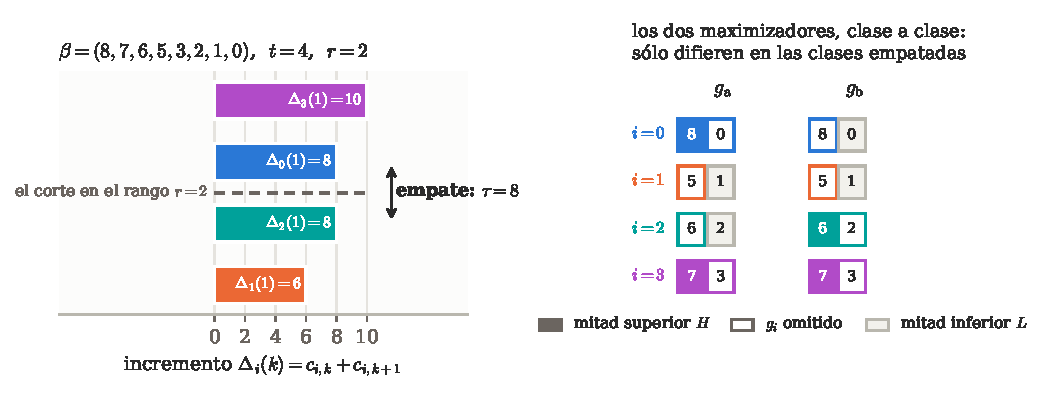
\includegraphics[width=\textwidth]{fig_increments_es.pdf}
\caption{El Teorema \ref{thm:Ggen} hecho sobre una forma, en vez de enunciado. Para
$\beta=(8,7,6,5,3,2,1,0)$ con $t=4$, $r=2$ las cuatro clases de exceso son $\{8,0\}$, $\{5,1\}$,
$\{6,2\}$, $\{7,3\}$ y los cuatro incrementos son $\Delta_3(1)=10$, $\Delta_0(1)=8$,
$\Delta_2(1)=8$, $\Delta_1(1)=6$. Un maximizador toma los $r=2$ mayores; el segundo y el tercero son
iguales, así que $\tau=\Delta_{(2)}=\Delta_{(3)}=8$ y hay exactamente dos. La pareja empatada
pertenece a las clases $0$ y $2=0+t/2$, que es \eqref{eq:congrgen} y no una casualidad: ningún valor
lo comparten incrementos de clases distintas de $i$ e $i+t/2$. A la derecha los dos maximizadores
están dibujados clase a clase en la forma de prefijo del Paso 2 --- leyendo una clase en orden
decreciente, primero los elementos de la mitad de arriba, luego el omitido $g_i$, luego los de la
mitad de abajo ---, lo que hace visible que difieren en las clases empatadas y en ninguna otra. El
color codifica la clase, no el rango. Calculada por \texttt{anc/fig\_v2.py}.}
\label{fig:increments}
\end{figure}

\begin{corollary}[un maximizador único]\label{cor:uniquegen}
Si $|G|=1$ entonces $\Phi_{t,r}\not\equiv0$.
\end{corollary}

\begin{proof}
Por \eqref{eq:topgen} la componente del numerador en grado $D_1$ es $\pm V\,P(T_g)\ne0$ para el único
$g$. Un polinomio de Laurent con una componente homogénea no nula no es nulo, así que el numerador no
es nulo y por tanto tampoco lo es $\Phi_{t,r}$.
\end{proof}

\begin{corollary}[el bloque central]\label{cor:midgen}
Escríbase $\mathcal{S}=\{s_1>\dots>s_n\}$, $n=2r+e$. Si el bloque $\{s_{r+1},\dots,s_{r+e}\}$
contiene exactamente un elemento de cada clase de exceso, entonces $\Phi_{t,r}\not\equiv0$.
\end{corollary}

\begin{proof}
$\deg(\mathcal{S}\setminus g)\le(s_1+\dots+s_r)-(s_{n-r+1}+\dots+s_n)$, porque los $r$ elementos
mayores de $\mathcal{S}\setminus g$ están dominados término a término por $s_1,\dots,s_r$ y sus $r$
menores dominan a $s_{n-r+1},\dots,s_n$. La igualdad obliga a que $\mathcal{S}\setminus g$ contenga
los dos bloques extremos, es decir $g\subseteq\{s_{r+1},\dots,s_{r+e}\}$, y $|g|=e$ fuerza la igualdad
de los dos conjuntos. Así que la cota la alcanza exactamente un término y se aplica el Corolario
\ref{cor:uniquegen}.
\end{proof}

\begin{corollary}[$t$ impar]\label{cor:oddgen}
Sea $t$ impar y $r\ge1$. Entonces $\Phi_{t,r}(\lambda;z)\equiv0$ si y sólo si alguna clase de residuos
módulo $t$ está ausente de $\beta(\lambda)$.
\end{corollary}

\begin{proof}
Si algún $n_i=0$ entonces $\mathcal T=\varnothing$ en el Lema \ref{lem:L3gen} y el numerador se anula.
Recíprocamente, si todos los $n_i\ge1$ entonces $|G|=1$ por el Teorema \ref{thm:Ggen}(c) y se aplica
el Corolario \ref{cor:uniquegen}.
\end{proof}

\begin{remark}
Para $r=1$ el Corolario \ref{cor:oddgen} es la Proposición \ref{rem:lattice}, demostrada allí viendo
que la cláusula concéntrica es vacua para $t$ impar --- un argumento interno al perfil de dos clases
que fuerza un solo par recíproco. Lo nuevo es que el enunciado sobrevive para todo $r\ge1$, y por una
ruta que no menciona el perfil en absoluto: la congruencia \eqref{eq:congrgen}. En $r=0$ es falso,
puesto que la regla de Littlewood da $s_\lambda(\zt)=0$ siempre que el $t$-núcleo es no vacío, $t$
impar incluido; y la observación de que $\prod\zt=+1$ para $t$ impar no lo entrega por sí sola,
porque el alfabeto es un subtoro de dimensión $r$ con las coordenadas restantes congeladas.
\end{remark}

% ---- v2_block3_es.tex ----
\subsection{El criterio en \texorpdfstring{$t=2$}{t=2}: rigidez y reflexión}\label{sec:rigidity}

El Corolario \ref{cor:uniquegen} resuelve toda forma con un maximizador único. Lo que sigue es la
otra mitad: cuando $|G|=2$, los dos términos de \eqref{eq:topgen} sólo pueden cancelarse si las dos
transversales son reflexión una de otra, y esa rigidez la aporta un único resultado ajeno.

\begin{theorem}[Purbhoo--van Willigenburg {\cite[Thm.~2.5]{PvW}}]\label{thm:PvW}
Para particiones con a lo sumo $n$ partes, escribiendo $\lambda^{-}:=\lambda/(\lambda_n)^{n}$,
\[
  s_\lambda(x_1,\dots,x_n)\,s_\mu(x_1,\dots,x_n)=s_\nu(x_1,\dots,x_n)\,s_\rho(x_1,\dots,x_n)
\]
si y sólo si $\lambda_n+\mu_n=\nu_n+\rho_n$ y $\{\lambda^{-},\mu^{-}\}=\{\nu^{-},\rho^{-}\}$ como
multiconjuntos.
\end{theorem}

\begin{remark}
El Teorema 3 de \cite{Rajan} da el enunciado para $n$ factores, pero bajo la hipótesis de que todos
los pesos máximos sean no nulos. El Teorema \ref{thm:PvW} no necesita tal hipótesis, y por eso es el
que usamos aquí: el caso degenerado, un factor trivial, es exactamente lo que produce el Lema
\ref{lem:dictgen} siempre que $\alpha^{*}$ o $\tilde\alpha$ es vacía. Ninguno de los dos enunciados
puede atajarse por factorización única, ya que los polinomios de Schur no son irreducibles:
$s_{(3)}(x,y)=(x+y)(x^2+y^2)$.
\end{remark}

\subsubsection*{El diccionario}

Escríbase $T=(u_1>\dots>u_{2r})$ con mitades $H=(h_1>\dots>h_r)$ y $L=(l_1>\dots>l_r)$, sea
$\delta=(r-1,r-2,\dots,0)$, de modo que $a_\delta(z)=\det(z_j^{\,r-i})$ es el determinante de
Vandermonde en la notación de la \S\ref{sec:extremal}, y póngase
\[
  \alpha=H-\delta,\qquad \tilde\alpha=\alpha-(\alpha_r)^{r},\qquad
  L^{*}=(l_1-l_r>\dots>l_1-l_1),\qquad \alpha^{*}=L^{*}-\delta .
\]

\begin{lemma}[el diccionario]\label{lem:dictgen}
$\alpha^{*}_r=0$ y
\begin{equation}\label{eq:dictgen}
  P(T)\;=\;(-1)^{\binom r2}\Bigl(\textstyle\prod_j z_j\Bigr)^{h_r-l_1}
  a_\delta(z)^2\,s_{\tilde\alpha}(z)\,s_{\alpha^{*}}(z).
\end{equation}
En particular $P$ no cambia bajo $T\mapsto T+m$ ni, por el Lema \ref{lem:reflgen}, bajo
$T\mapsto c-T$.
\end{lemma}

\begin{proof}
$a_H(z)=s_\alpha(z)a_\delta(z)$ es la fórmula bialternante. Para el segundo factor, multiplicar la
columna $j$ de $\det(z_j^{-l_i})$ por $z_j^{l_1}$ da
$(\prod_j z_j^{l_1})a_L(z^{-1})=\det(z_j^{\,l_1-l_i})$, cuyos exponentes de fila crecen con $i$;
invertir las $r$ filas cuesta $(-1)^{\binom r2}$ y produce $a_{L^{*}}(z)=s_{\alpha^{*}}(z)a_\delta(z)$.
Finalmente $s_\alpha=(\prod_j z_j)^{\alpha_r}s_{\tilde\alpha}$ y $\alpha_r=h_r$.
\end{proof}

\begin{proposition}[la órbita de $P$]\label{prop:orbitgen}
Sean $T,\widetilde T$ conjuntos de $2r$ enteros distintos con $P(T)=\pm P(\widetilde T)$. Entonces
$\widetilde T=T+m$ para algún $m\in\ZZ$, o bien $\widetilde T=c-T$ para algún $c\in\ZZ$.
\end{proposition}

\begin{proof}
Dos observaciones primero. El signo es $+$: por \eqref{eq:dictgen} los dos lados son un monomio por
$a_\delta^2$ por un producto de dos polinomios de Schur, que tiene coeficientes no negativos, así que
un signo menos es imposible. Y el monomio hay que reabsorberlo: con $d=h_r-l_1\ge1$, lo que se cumple
porque $T$ es estrictamente decreciente, $(\prod_j z_j)^{d}s_{\tilde\alpha}=s_{\tilde\alpha+(d^{r})}$,
y es ese $d$ el que hace el papel de $\lambda_n+\mu_n$ en el Teorema \ref{thm:PvW}, estando
$\alpha^{*}$ ya normalizada. Cancelando $a_\delta^2$ y aplicando el Teorema \ref{thm:PvW} con $n=r$ a
$(\lambda,\mu)=(\tilde\alpha+(d^{r}),\alpha^{*})$ y al par correspondiente $(\nu,\rho)$ de
$\widetilde T$, el criterio dice que el entero $d$ coincide y que $\{\tilde\alpha,\alpha^{*}\}$
coincide como multiconjunto. Coincidir en el mismo orden dice que $H,\widetilde H$ y $L,\widetilde L$
son trasladados, y la igualdad de los dos enteros $d$ fuerza la misma traslación en las dos mitades,
es decir $\widetilde T=T+m$. Coincidir tras intercambiar dice que $H$ es, salvo traslación, la
inversa de $\widetilde L$ y $L$ la de $\widetilde H$, es decir $\widetilde T=c-T$.
\end{proof}

\subsubsection*{Los dos maximizadores se reflejan}

De aquí al final de la subsección supóngase $|G|=2$ y escríbase
$G=\{g_{\mathrm a},g_{\mathrm b}\}$, $T_{\mathrm a}=\mathcal{S}\setminus g_{\mathrm a}$,
$T_{\mathrm b}=\mathcal{S}\setminus g_{\mathrm b}$, con mitades
$T_{\mathrm a}=H_{\mathrm a}\sqcup L_{\mathrm a}$ y $T_{\mathrm b}=H_{\mathrm b}\sqcup L_{\mathrm b}$,
y
\[
  \mathcal{K}=T_{\mathrm a}\cap T_{\mathrm b}.
\]
Por el Teorema \ref{thm:Ggen}(b) las dos transversales difieren exactamente en las clases empatadas
$i$ e $i'=i+t/2$, digamos
\begin{equation}\label{eq:swapgen}
  g_{\mathrm a}\ni p_1=c_{i,k+1},\ q_1=c_{i',k'},\qquad
  g_{\mathrm b}\ni p_2=c_{i,k},\ q_2=c_{i',k'+1},
\end{equation}
de modo que $p_1+p_2=q_1+q_2=\tau$ por \eqref{eq:incrgen}: el valor del empate es la suma de cada
pareja intercambiada.

\begin{proposition}[la traslación fuerza la reflexión]\label{prop:translgen}
Si $T_{\mathrm b}=T_{\mathrm a}+m$ con $m\ne0$, entonces $T_{\mathrm b}=\tau-T_{\mathrm a}$.
\end{proposition}

\begin{proof}
$|T_{\mathrm a}\cap(T_{\mathrm a}+m)|=|\mathcal{K}|=2r-2$. Póngase una arista $x\to x+m$ cuando $x$ y
$x+m$ estén los dos en $T_{\mathrm a}$; como $m\ne0$, cada vértice tiene a lo sumo una arista
saliente y una entrante, así que el grafo es una unión disjunta de caminos dirigidos. Tiene $2r$
vértices y, por el cardinal anterior, exactamente $2r-2$ aristas, luego exactamente dos componentes.
Así que $T_{\mathrm a}$ es unión de exactamente dos progresiones aritméticas maximales de paso $m$,
digamos $T_{\mathrm a}=\{p,p+m,\dots,p+(u-1)m\}\cup\{q,\dots,q+(v-1)m\}$ con $u+v=2r$. Entonces
$T_{\mathrm a}\setminus T_{\mathrm b}=\{p,q\}$ y $T_{\mathrm b}\setminus T_{\mathrm a}=\{p+um,q+vm\}$.
El empate dice que $x\mapsto\tau-x$ lleva la primera pareja sobre la segunda, y hay dos
emparejamientos. Si $\tau-p=p+um$ y $\tau-q=q+vm$ entonces
$\tau-T_{\mathrm a}=\{p+m,\dots,p+um\}\cup\{q+m,\dots,q+vm\}=T_{\mathrm b}$. Si $\tau-p=q+vm$ y
$\tau-q=p+um$, restando queda $um=vm$, luego $u=v$, y otra vez
$\tau-T_{\mathrm a}=T_{\mathrm b}$.
\end{proof}

\begin{proposition}[el centro es el valor del empate]\label{prop:centregen}
Si $T_{\mathrm b}=c-T_{\mathrm a}$ entonces $c=\tau$.
\end{proposition}

\begin{proof}
$x\mapsto c-x$ es una involución que lleva $T_{\mathrm a}$ a $T_{\mathrm b}$, luego $T_{\mathrm b}$ a
$T_{\mathrm a}$, luego $\mathcal{K}$ a $\mathcal{K}$; por tanto lleva
$T_{\mathrm a}\setminus\mathcal{K}$ sobre $T_{\mathrm b}\setminus\mathcal{K}$. Por \eqref{eq:swapgen}
esos dos conjuntos son $T_{\mathrm a}\setminus\mathcal{K}=\{p_2,q_2\}$ y
$T_{\mathrm b}\setminus\mathcal{K}=\{p_1,q_1\}$, ya que $T_{\mathrm a}$ omite exactamente $p_1,q_1$ y
$T_{\mathrm b}$ omite exactamente $p_2,q_2$. O bien $c-p_2=p_1$, y entonces $c-q_2=q_1$, de donde
$c=p_1+p_2=\tau$; o bien $c-p_2=q_1$ y $c-q_2=p_1$, y sumando queda
$2c=p_1+p_2+q_1+q_2=2\tau$, otra vez $c=\tau$. En el segundo caso además
$c=p_2+q_1\equiv i+i'\equiv2i+t/2$ mientras que $\tau\equiv2i$ por \eqref{eq:congrgen}, así que
$c=\tau$ forzaría $t/2\equiv0\pmod t$, imposible para $t\ge2$: el emparejamiento cruzado no ocurre.
\end{proof}

\begin{corollary}[la reflexión]\label{cor:reflectgen}
Si $\bigl[\det(x_i^{\beta_j})\bigr]_{D_1}=0$ entonces $|G|=2$ y $T_{\mathrm b}=\tau-T_{\mathrm a}$.
En consecuencia $\tau-\mathcal{K}=\mathcal{K}$ y, como $x\mapsto\tau-x$ también fija $\{p_1,p_2\}$ y
$\{q_1,q_2\}$ como conjuntos,
\begin{equation}\label{eq:Ssymgen}
  \tau-\bigl(\mathcal{K}\cup\{p_1,p_2,q_1,q_2\}\bigr)=\mathcal{K}\cup\{p_1,p_2,q_1,q_2\}.
\end{equation}
\end{corollary}

\begin{proof}
$|G|=1$ queda excluido por el Corolario \ref{cor:uniquegen}. Con $|G|=2$, \eqref{eq:topgen} y
$w(g)=\pm1$ dan $P(T_{\mathrm a})=\pm P(T_{\mathrm b})$; se aplica la Proposición
\ref{prop:orbitgen} y luego las Proposiciones \ref{prop:translgen} y \ref{prop:centregen}. La
identidad $\tau-\mathcal{K}=\mathcal{K}$ es la primera línea de la prueba de la Proposición
\ref{prop:centregen}, y $p_1+p_2=q_1+q_2=\tau$ es el empate.
\end{proof}

\begin{remark}[tres constantes fáciles de confundir]
$\tau=\Delta_{(r)}$ es el valor del empate, un dato del algoritmo voraz ajeno a toda simetría; $c$ es
un centro de reflexión, producido por la rigidez y sin nada que ver con los residuos;
$C=\min\mathcal{S}+\max\mathcal{S}$ es un estadístico del beta-conjunto, y es el que usa la condición
\textup{(ii)}. Que $c=\tau$ \textup{(}Proposición \ref{prop:centregen}\textup{)} y que $C=\tau$
\textup{(}Corolario \ref{cor:Ctaugen}\textup{)} son teoremas, no notación, y los dos necesitan la
hipótesis de anulación: escribir $C$ donde corresponde $\tau$ demuestra menos de lo que parece.
Nosotros cometimos ese desliz; de ahí los tres símbolos.
\end{remark}

\subsubsection*{El centro del beta-conjunto}

Los dos maximizadores coinciden fuera de las clases empatadas, así que su parte omitida común
\begin{equation}\label{eq:gcomgen}
  g_{\mathrm{com}}:=g_{\mathrm a}\cap g_{\mathrm b},\qquad
  \mathcal{S}=\mathcal{K}\ \sqcup\ g_{\mathrm{com}}\ \sqcup\ \{p_1,p_2,q_1,q_2\}
\end{equation}
es vacía exactamente cuando $e=2$. Por \eqref{eq:Ssymgen} el conjunto
$\mathcal{S}\setminus g_{\mathrm{com}}$ es estable bajo $x\mapsto\tau-x$, pero $g_{\mathrm{com}}$ no
tiene por qué serlo, así que $\mathcal{S}$ tampoco. Eso es más de lo que hace falta: sólo los dos
\emph{extremos} de $\mathcal{S}$ tienen que evitar $g_{\mathrm{com}}$, y lo hacen. La Figura
\ref{fig:reflection} dibuja tanto la reflexión como la forma que tiene $|G|=2$ sin ella, que es lo
que la proposición siguiente debe excluir.

\begin{figure}[!ht]
\centering
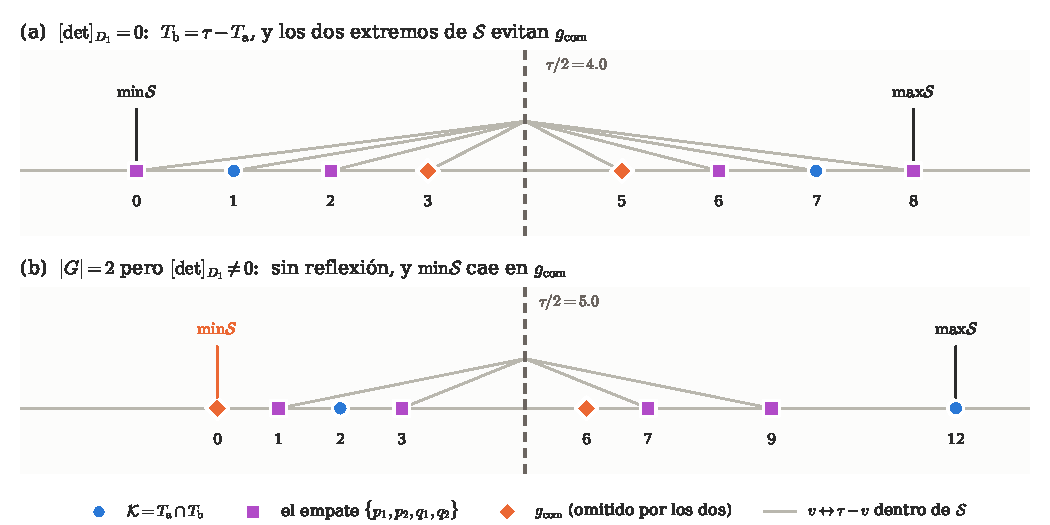
\includegraphics[width=\textwidth]{fig_reflection_es.pdf}
\caption{El Corolario \ref{cor:reflectgen} y la Proposición \ref{prop:A1gen} sobre dos formas, las
dos con $t=4$, $r=2$ y $|G|=2$. Cada panel dibuja $\mathcal{S}$ sobre una recta, coloreada según a
qué parte de \eqref{eq:gcomgen} pertenece el valor; un arco une $v$ con $\tau-v$ cuando los dos están
en $\mathcal{S}$, y la línea discontinua es el centro $\tau/2$. \emph{(a)} $\beta=(8,7,6,5,3,2,1,0)$:
$\tau=8$, $\mathcal{K}=\{1,7\}$, $g_{\mathrm{com}}=\{3,5\}$, empate $\{0,2,6,8\}$. Aquí
$T_{\mathrm b}=\tau-T_{\mathrm a}$, así que $\mathcal{S}\setminus g_{\mathrm{com}}$ es simétrico
respecto de $\tau/2$, y los dos extremos de $\mathcal{S}$ evitan $g_{\mathrm{com}}$, luego
$C=0+8=\tau$. Aquí $g_{\mathrm{com}}=\{3,5\}$ resulta ser simétrico también ---el arco que une sus
dos miembros se dibuja como cualquier otro---, que es lo que la Conjetura \ref{conj:gcom} afirma en
general y lo que la \S\ref{sec:rigidity} no demuestra: la reflexión queda establecida sobre
$\mathcal{S}\setminus g_{\mathrm{com}}$ y observada en el resto.
\emph{(b)} $\beta=(12,9,7,6,3,2,1,0)$: aquí $\tau=10$, y otra vez $|G|=2$, pero los dos maximizadores no
son reflexión uno de otro; $\min\mathcal{S}=0$ cae en $g_{\mathrm{com}}$, y $C=0+12=12\neq\tau$. El
panel (b) es la razón de que la Proposición \ref{prop:A1gen} no pueda demostrarse sólo a partir de
$|G|=2$. Calculada por \texttt{anc/fig\_v2.py}.}
\label{fig:reflection}
\end{figure}


\begin{proposition}[los extremos evitan la parte común]\label{prop:A1gen}
Supóngase $\bigl[\det(x_i^{\beta_j})\bigr]_{D_1}=0$. Entonces
$\max\mathcal{S}\notin g_{\mathrm{com}}$ y $\min\mathcal{S}\notin g_{\mathrm{com}}$.
\end{proposition}

\begin{proof}
Por el Corolario \ref{cor:reflectgen}, $T_{\mathrm b}=\tau-T_{\mathrm a}$. Como $x\mapsto\tau-x$
invierte el orden, lleva la mitad de abajo de $T_{\mathrm a}$ a la de arriba de $T_{\mathrm b}$ y al
revés:
\begin{equation}\label{eq:halvesgen}
  H_{\mathrm b}=\tau-L_{\mathrm a},\qquad L_{\mathrm b}=\tau-H_{\mathrm a}.
\end{equation}
Recuérdese del Paso 2 de la prueba del Teorema \ref{thm:Ggen} que un maximizador queda descrito por
los enteros $k_i$: dentro de la clase $i$, leída en orden decreciente, los primeros $k_i$ valores de
exceso están en la mitad de arriba, el siguiente es el omitido $g_i$, y los restantes están en la
mitad de abajo. Recuérdese también del Teorema \ref{thm:Ggen}(a) que un maximizador selecciona todo
incremento $>\tau$, que los incrementos de una clase se seleccionan en orden de prefijo, y que los
únicos incrementos iguales a $\tau$ son los dos empatados, que viven en las dos clases empatadas.

\emph{El máximo.} Póngase $m=\max\mathcal{S}$ y sea $i$ su clase, de modo que $m=c_{i,1}$ y
$n_i\ge2$; escríbase $c=c_{i,2}$. Entonces $m\in g_{\mathrm a}\cap g_{\mathrm b}$ si y sólo si
$k_i=0$ en los dos maximizadores. Supóngase que sí. Entonces la clase $i$ no está empatada: un
maximizador que toma el incremento empatado de una clase empatada tiene allí $k_i\ge1$. Luego ningún
incremento de la clase $i$ es $\ge\tau$ y, en particular,
\[
  \Delta_i(1)=m+c<\tau .
\]
Por otro lado $k_i=0$ coloca $c$ en la mitad de abajo de los dos maximizadores, así que
$c\in L_{\mathrm b}$, y \eqref{eq:halvesgen} da $\tau-c\in H_{\mathrm a}\subseteq\mathcal{S}$, de
donde $\tau-c\le\max\mathcal{S}=m$, esto es $\tau\le m+c$. Las dos desigualdades mostradas se
contradicen.

\emph{El mínimo} es la imagen especular. Póngase $m^{-}=\min\mathcal{S}$, sea $i^{-}$ su clase,
$n=n_{i^{-}}\ge2$ y $c'=c_{i^{-},n-1}$, de modo que $m^{-}=c_{i^{-},n}$. Entonces
$m^{-}\in g_{\mathrm a}\cap g_{\mathrm b}$ si y sólo si $k_{i^{-}}=n-1$ en los dos, es decir si y
sólo si los dos maximizadores seleccionan \emph{todos} los incrementos de la clase $i^{-}$; otra vez
la clase $i^{-}$ no puede estar empatada, ya que el maximizador que no toma el incremento empatado de
una clase empatada omite allí uno. Luego todo incremento de la clase $i^{-}$ supera a $\tau$, en
particular $\Delta_{i^{-}}(n-1)=m^{-}+c'>\tau$. Y $k_{i^{-}}=n-1$ coloca $c'$ en la mitad de arriba
de los dos, así que $c'\in H_{\mathrm b}$, y \eqref{eq:halvesgen} da
$\tau-c'\in L_{\mathrm a}\subseteq\mathcal{S}$, de donde $\tau-c'\ge\min\mathcal{S}=m^{-}$, esto es
$\tau\ge m^{-}+c'$. Contradicción.
\end{proof}

\begin{corollary}[el centro es el valor del empate]\label{cor:Ctaugen}
Si $\bigl[\det(x_i^{\beta_j})\bigr]_{D_1}=0$ entonces $C:=\min\mathcal{S}+\max\mathcal{S}=\tau$, y
$\mathcal{S}$ corta a todas las clases de residuos de las dos empatadas. Además $t$ es par y las dos
clases empatadas son exactamente las dos soluciones de $2\kappa\equiv C\pmod t$, ambas en
$\mathcal{E}$.
\end{corollary}

\begin{proof}
Por \eqref{eq:Ssymgen} el conjunto $\mathcal{S}\setminus g_{\mathrm{com}}$ es estable bajo
$x\mapsto\tau-x$, así que su mayor y su menor elemento suman $\tau$; por la Proposición
\ref{prop:A1gen} los dos extremos de $\mathcal{S}$ están en ese conjunto, luego \emph{son} su mayor y
su menor elemento, y $C=\tau$. El Teorema \ref{thm:Ggen}(b) da $t$ par y las dos clases empatadas
$i,i+t/2$, ambas en $\mathcal{E}$; por \eqref{eq:congrgen} $\tau\equiv2i\pmod t$, así que
$2\kappa\equiv\tau=C$ tiene exactamente las dos soluciones $\kappa=i$ y $\kappa=i+t/2$.
\end{proof}

\begin{corollary}[una condición necesaria, para todo $t$ par y todo $r$]\label{cor:necgen}
Sean $t\ge2$ y $r\ge1$, y supongamos $\Phi_{t,r}(\lambda;z)\equiv0$ con todo $n_i\ge1$. Entonces $t$
es par, $|G|=2$, $\min\mathcal{S}+\max\mathcal{S}=\tau$, y $\mathcal{S}\setminus g_{\mathrm{com}}$ es
simétrico respecto de $\tau/2$.
\end{corollary}

\begin{proof}
$\Phi_{t,r}$ y el numerador difieren en un factor no nulo, así que el numerador se anula
idénticamente y en particular $\bigl[\det(x_i^{\beta_j})\bigr]_{D_1}=0$. Se aplican los Corolarios
\ref{cor:reflectgen} y \ref{cor:Ctaugen} y \eqref{eq:Ssymgen}.
\end{proof}

\noindent Esto es lo que sobrevive de las \S\S\ref{sec:extremal}--\ref{sec:rigidity} fuera de $t=2$.
Lo que \emph{no} da es el paso que cierra $t=2$: allí $e=2$ obliga a $g_{\mathrm{com}}=\varnothing$, y
la simetría de $\mathcal{S}\setminus g_{\mathrm{com}}$ pasa a ser la simetría del propio $\beta$. Para
$t\ge4$ la parte común $g_{\mathrm{com}}$ puede no ser vacía, y el argumento de arriba no dice nada
de ella: la reflexión queda establecida sólo sobre $\mathcal{S}\setminus g_{\mathrm{com}}$, de modo
que restringe a $\beta$ sin llegar a determinarlo. Que $g_{\mathrm{com}}$ sea simétrico también es lo
que muestran las medidas y lo que enuncia la Conjetura \ref{conj:gcom}; aquí no se demuestra.

\subsubsection*{La condición es suficiente, para todo \texorpdfstring{$t$}{t} y todo
\texorpdfstring{$r$}{r}}

Una condición necesaria invita a su recíproco, y la mitad se consigue de una pieza. La reflexión que
el Corolario \ref{cor:necgen} extrae del estrato superior resulta ser, cuando vale sobre todo
$\mathcal{S}$ y no sólo sobre una parte, una simetría de \emph{cada} término de la suma de Laplace y
no únicamente de los dos maximizadores; y una involución sin puntos fijos cancela lo que empareja.
Escribimos
\[
C:=\min\mathcal{S}+\max\mathcal{S},\qquad\text{y escribimos } x\mapsto C-x
\text{ para la reflexión que centra.}
\]

\begin{theorem}[la dirección suficiente, para todo $t$ y todo $r$]\label{thm:suff}
Sean $t\ge2$, $r\ge1$, $N=t+2r$, y supongamos ocupada toda clase de residuos. Supongamos que
\begin{equation}\label{eq:suffcond}
C-\mathcal{S}=\mathcal{S}
\qquad\text{y}\qquad
\Delta_i(k)=C\ \text{para algún } i\in\mathcal{E},\ k .
\end{equation}
Entonces $\Phi_{t,r}(\lambda;z)\equiv0$.
\end{theorem}

Las dos cláusulas hacen dos trabajos distintos, y conviene decir cuál es cuál antes de la prueba: la
primera hace que la reflexión \emph{actúe} sobre las transversales, y la segunda hace que esa acción
sea \emph{libre}. La Figura \ref{fig:pairing} es el mecanismo entero sobre una sola forma, con otra al
lado que cumple la primera cláusula y no la segunda.

\begin{figure}[!ht]
\centering
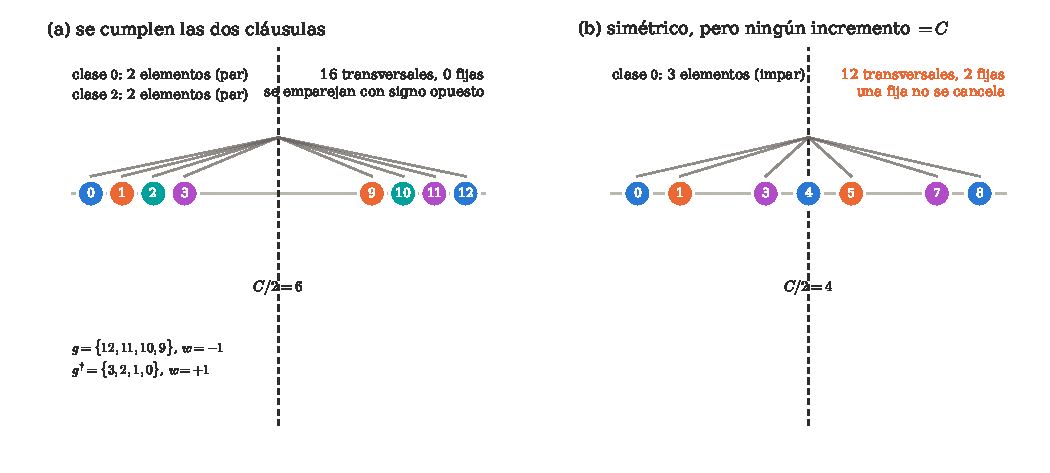
\includegraphics[width=\textwidth]{fig_pairing_es.pdf}
\caption{Por qué se cancela la suma, y para qué está la segunda cláusula. Cada panel dibuja
$\mathcal{S}$ sobre una recta, coloreado por clase de residuo, con un arco que une $v$ con $C-v$ y el
eje de puntos en $C/2$. \emph{(a)} $\beta=(12,11,10,9,3,2,1,0)$ con $t=4$, $r=2$: las dos clases que
la reflexión fija tienen tamaño \emph{par}, así que ninguna contiene a $C/2$; las $16$ transversales
se emparejan sin ningún punto fijo, y cada pareja lleva signos opuestos, de modo que cada término de
\eqref{eq:laplacegen} lo cancela otro. Una de esas parejas está impresa con sus dos signos,
calculados y no afirmados. \emph{(b)} una forma con $C-\mathcal{S}=\mathcal{S}$ pero sin ningún
incremento igual a $C$, encontrada buscándola y no elegida: allí la clase fija tiene tamaño
\emph{impar}, luego contiene a $C/2$, y dos transversales son su propio reflejo. Un término
emparejado consigo mismo no puede cancelarse, y la suma sobrevive. Eso es todo lo que compra la
segunda cláusula. Calculada por \texttt{anc/fig\_involution2.py}.}
\label{fig:pairing}
\end{figure}

\begin{lemma}[la transversal reflejada]\label{lem:reflact}
Supongamos $C-\mathcal{S}=\mathcal{S}$. Entonces $x\mapsto C-x$ lleva la clase $i$ sobre la clase
$i^{*}:=C-i \bmod t$, y o las dos están en $\mathcal{E}$ o ninguna; de modo que
\[
g^{\dagger}:=\bigl(C-(g\cap\mathcal{S})\bigr)\cup\bigl(g\setminus\mathcal{S}\bigr)
\]
es de nuevo una transversal, $g\mapsto g^{\dagger}$ es una involución sobre ellas, y
$T_{g^{\dagger}}=C-T_g$.
\end{lemma}

\begin{proof}
Todo elemento de la clase $i$ es $\equiv i$, así que $x\mapsto C-x$ lo manda dentro de la clase
$i^{*}$; como $C-\mathcal{S}=\mathcal{S}$ y la aplicación es inyectiva, lleva la clase $i$
\emph{sobre} la clase $i^{*}$ siempre que $i\in\mathcal{E}$, lo que obliga a $i^{*}\in\mathcal{E}$ y a
$n_i=n_{i^{*}}$. Las clases unitarias no se tocan: su único elemento está congelado en toda
transversal. Por último $T_{g^{\dagger}}=\mathcal{S}\setminus g^{\dagger}=C-(\mathcal{S}\setminus
g)=C-T_g$.
\end{proof}

\begin{lemma}[el menor reflejado]\label{lem:Arefl}
$A(C-T)=A(T)$ para todo $2r$-conjunto $T$ y todo $C$.
\end{lemma}

\begin{proof}
% Sin "=" en esta frase: TeX parte la formula en linea despues de la relacion y deja el signo
% colgando fuera del margen, y forzarla con \mbox la echa entera fuera.  Se dice con palabras.
Sacar $x_i^{C}$ de cada una de las $2r$ filas multiplica el determinante por el factor
$\prod_j z_j^{C}z_j^{-C}$, que vale $1$, y deja la matriz de $T$ con $x_i$ sustituido por
$x_i^{-1}$, que es la
matriz de $T$ con las dos filas de cada par recíproco intercambiadas: un signo $(-1)^{r}$.
Y listar $C-T$ en orden decreciente invierte el orden de las columnas, lo que aporta
$(-1)^{\binom{2r}{2}}$, es decir $(-1)^{r}$, porque $2r-1$ es impar. Los dos se cancelan.
\end{proof}

\noindent Los dos movimientos de esa prueba no son nuestros, y merece la pena decir de quién son,
porque son el instrumento adecuado y los elegimos por eso. Escalar cada fila por una potencia para
sustituir $x_i$ por $\bar x_i$, y luego invertir un bloque de columnas para recoger
$(-1)^{n(n-1)/2}$, es la maniobra que Ayyer y Behrend emplean sobre el bialternante de una forma
autocomplementaria \cite[\S3]{AB19}; ellos mismos describen sus pruebas como apoyadas sólo en las
expresiones determinantales ``y la aplicación de operaciones estándar con determinantes'', y ésta es
una de esas operaciones. Albion hace la misma inversión del lado de las raíces de la unidad
\cite{Alb23,Alb25}, y a nivel de caracteres el mismo hecho es la invariancia de $sp_\lambda$ bajo
$x_i\mapsto\bar x_i$, recogida en \cite{AB19} y puesta a trabajar en \cite{AF20}.

Conviene explicar por qué es útil aquí, porque es lo que hace corta toda la sección. A un menor
reflejado se le puede atacar desarrollándolo, y entonces habría que seguir término a término las
clases unitarias y las reflejadas --- que es como lo intentamos primero, y no se acaba nunca. La
maniobra de Ayyer y Behrend, en cambio, liquida la reflexión en \emph{dos} cálculos de signo que no
miran las entradas en ningún momento, y es robusta justo en el sentido que necesitamos: no usa en
ningún paso que se esté reflejando el alfabeto entero, así que sobrevive al aplicarse a una
\emph{parte} del conjunto beta, con el resto quieto. Esa robustez es la razón de que el Lema
\ref{lem:Arefl} ocupe cuatro líneas y no una sección, y pertenece a la herramienta y no a nosotros.
Es además un indicio menor a favor de la tesis de la \S\ref{sec:background}: las dos líneas entre las
que se sitúa este artículo comparten más maquinaria de lo que sus enunciados dejan ver.

El enunciado que sigue es el corazón combinatorio del argumento, y sólo necesita la primera cláusula
de \eqref{eq:suffcond}. Reflejar un conjunto beta \emph{entero} es clásico --- es la identidad de
complementación \eqref{eq:compl}, y los pasos determinantales que hay detrás son los estándar que
acabamos de citar. Lo que aquí se pide es la reflexión de la parte de exceso \emph{sola}, con las
clases unitarias quietas e intercaladas entre los valores reflejados; las dos involuciones que eso
produce, una de $\beta$ y otra de $\ZZ/t$, son de las que acaba dependiendo el signo.

\begin{lemma}[la fórmula del signo de la reflexión parcial]\label{lem:signformula}
Supongamos $C-\mathcal{S}=\mathcal{S}$, y pongamos
\[
\nu=\#\{x\in\mathcal{S}:2x=C\},\qquad \eta=\#\{i\in\mathcal{E}:2i\equiv C \bmod t\}.
\]
Entonces, para toda transversal $g$,
\begin{equation}\label{eq:wrefl}
\frac{w(g^{\dagger})}{w(g)}\;=\;(-1)^{\,e-\frac{\nu+\eta}{2}} .
\end{equation}
En particular el cociente no depende de $g$, ni de $r$, ni de $N$.
\end{lemma}

\begin{corollary}\label{cor:whenminus}
Bajo $C-\mathcal{S}=\mathcal{S}$, el cociente \eqref{eq:wrefl} vale $-1$ si y sólo si $\eta=2$.
\end{corollary}

\begin{proof}
Una involución tiene tantos puntos fijos como elementos su conjunto, módulo dos, así que
$\nu\equiv|\mathcal{S}|$ y $\eta\equiv e$; y $|\mathcal{S}|=2r+e$ por \eqref{eq:excessgen}, luego
también $\nu\equiv e$. Si $e$ es impar, entonces $\nu=\eta=1$ y el exponente es $e-1$, par. Si $e$ es
par, entonces $\nu=0$ y $\eta$ vale $0$ ó $2$, lo que da el exponente $e$ ó $e-1$; el primero es par y
el segundo impar.
\end{proof}

\noindent Esa independencia es la parte que parece improbable y es justo la que importa: las clases
unitarias están colocadas en posiciones arbitrarias entre los valores reflejados, y mover una
transversal las hace cruzarse unas con otras --- pero cada cruce que aportan a la suma de columnas lo
deshace el cruce que aportan a la palabra de residuos, así que no dejan rastro en el cociente.

\begin{lemma}[el signo reflejado]\label{lem:signrefl}
Supongamos \eqref{eq:suffcond}. Entonces $\eta=2$, el número $e$ es par, $\nu=0$, y
$w(g^{\dagger})=-w(g)$ para toda transversal $g$.
\end{lemma}

\begin{proof}[Prueba del Lema \ref{lem:signformula}]
Sea $\mathcal{R}$ la aplicación $x\mapsto C-x$ sobre $\mathcal{S}$ y la identidad sobre
$\beta\setminus\mathcal{S}$, y sea $\mathcal{R}_t$ la aplicación $i\mapsto i^{*}$ sobre $\mathcal{E}$
y la identidad fuera; ambas son involuciones, de $\beta$ y de $\ZZ/t$ respectivamente, con $\nu$ y
$\eta$ puntos fijos, así que $\sgn(\mathcal{R})=(-1)^{(|\mathcal{S}|-\nu)/2}$ y
$\sgn(\mathcal{R}_t)=(-1)^{(e-\eta)/2}$. Ordenemos las columnas de una transversal $g$ por residuo y
las restantes por $\beta$ decreciente; el signo de la permutación de $\{1,\dots,N\}$ que resulta es
$w(g)$ salvo un factor que depende sólo de $t$. Aplicar $\mathcal{R}$ a esa notación de una línea
aporta $\sgn(\mathcal{R})$; restablecer el orden por residuo del primer bloque aporta
$\sgn(\mathcal{R}_t)$; y $\mathcal{R}$ invierte $T_g$ por completo, de modo que restablecer su orden
decreciente aporta $(-1)^{\binom{2r}{2}}$. Multiplicando los tres sale \eqref{eq:wrefl}, donde ningún
término se refiere a $g$.
\end{proof}

\begin{proof}[Prueba del Lema \ref{lem:signrefl}]
Contar puntos fijos de una involución da $|\mathcal{S}|\equiv\nu$ y $e\equiv\eta \pmod 2$, y
$|\mathcal{S}|=2r+e$ por \eqref{eq:excessgen}, luego $e\equiv\nu$. Ahora bien, la segunda cláusula de
\eqref{eq:suffcond} dice que dos elementos \emph{adyacentes} de alguna clase $i_0$ suman $C$; la
reflexión los intercambia, así que $i_0=i_0^{*}$, y escribiendo la clase en orden decreciente el
intercambio manda su $k$-ésima entrada a la $(n_{i_0}+1-k)$-ésima, de donde $n_{i_0}=2k$ es par. La
reflexión $x\mapsto C-x$ tiene a lo sumo un punto fijo, que es $C/2$; como esta clase es estable bajo
ella y tiene cardinal par, sus elementos se emparejan y no contiene ninguno, luego $C/2\notin$ clase
$i_0$.

Antes de hablar de una segunda solución hay que saber que la hay, y ahí es donde la paridad de $t$ se
decide en vez de suponerse. Supongamos $t$ impar. Entonces $2$ es invertible módulo $t$, así que
$i\mapsto i^{*}$ tiene a $i_0$ como su \emph{único} residuo fijo; las demás clases de $\mathcal{E}$ se
emparejan, luego $e$ es impar, y $|\mathcal{S}|=2r+e$ también. Una involución sobre un conjunto de
tamaño impar tiene un punto fijo, así que $\nu=1$ y $C/2\in\mathcal{S}$; su residuo $\kappa$ cumple
$2\kappa\equiv C$, luego $\kappa=i_0$, lo que sitúa a $C/2$ en la clase $i_0$ --- que acabamos de ver
que no lo contiene. Así que $t$ es par, y $2i\equiv C$ tiene exactamente las dos soluciones $i_0$ e
$i_1=i_0+t/2$.

Si $\nu=1$, entonces $C/2\in\mathcal{S}$ y su residuo es $i_0$ o $i_1$; no es $i_0$, luego
$i_1\in\mathcal{E}$. Si $\nu=0$, entonces $e$ es par, y $\mathcal{E}=\{i_0\}\sqcup\{\text{pares}\}$
haría $e$ impar salvo que $i_1\in\mathcal{E}$. En cualquiera de los dos casos $\eta=2$, luego $e$ es
par y $\nu=0$, y el Corolario \ref{cor:whenminus} da el signo de inmediato. Leyendo \eqref{eq:wrefl}
directamente, el exponente es $e-\tfrac{0+2}2=e-1\equiv1 \pmod 2$.
\end{proof}

\begin{corollary}[la hipótesis, leída sobre los residuos]\label{cor:suffgeom}
Supongamos $C-\mathcal{S}=\mathcal{S}$. Entonces algún $\Delta_i(k)=C$ si y sólo si $t$ es par y
\emph{las dos} soluciones de $2i\equiv C \pmod t$ son clases de exceso. Dicho de otro modo,
\eqref{eq:suffcond} afirma: la parte de exceso del conjunto beta es simétrica respecto de $C/2$, y las
dos clases de residuos que la reflexión fija son ambas de exceso.
\end{corollary}

\begin{proof}
Una dirección es el primer párrafo de la prueba del Lema \ref{lem:signrefl}. Para la otra, si las dos
clases fijas están en $\mathcal{E}$ entonces $\eta=2$, luego $e$ es par por $e\equiv\eta$, luego
$|\mathcal{S}|=2r+e$ es par y $\nu=0$: ningún elemento de $\mathcal{S}$ queda fijo. Una clase fija es
entonces estable por la reflexión y sin puntos fijos, luego de tamaño par $2k$, y sus entradas
$k$-ésima y $(k+1)$-ésima se intercambian, así que $\Delta_i(k)=C$.
\end{proof}

\noindent Leída así, la hipótesis tiene la misma forma que la conclusión del Corolario
\ref{cor:Ctaugen}, y eso es lo que hace que las dos mitades de la sección se miren la una a la otra:
allí las dos clases empatadas \emph{resultan} ser las dos soluciones de $2\kappa\equiv C$; aquí
\emph{pedimos} que sean de exceso.

\begin{proof}[Prueba del Teorema \ref{thm:suff}]
Por el Lema \ref{lem:reflact}, $g\mapsto g^{\dagger}$ es una involución sobre las transversales con
$T_{g^{\dagger}}=C-T_g$. No tiene puntos fijos: una transversal fija necesitaría $C-g_i=g_i$, es
decir $g_i=C/2$, en toda clase con $i=i^{*}$, y la clase $i_0$ de la prueba anterior es una de ésas y
no contiene a $C/2$. Por los Lemas \ref{lem:Arefl} y \ref{lem:signrefl},
\[
w(g)A(T_g)+w(g^{\dagger})A(T_{g^{\dagger}})=w(g)A(T_g)-w(g)A(C-T_g)=0 ,
\]
así que la suma de \eqref{eq:laplacegen} se cancela por parejas y el numerador se anula
idénticamente.
\end{proof}

\begin{remark}[qué es esto, y qué no es]\label{rem:suffscope}
Conviene separar tres cosas. Primera: en $t=2$ la hipótesis \eqref{eq:suffcond} \emph{es} la rama
{\rm(b)}; allí $e=2$ obliga a $\mathcal{S}=\beta$, con lo que $C-\mathcal{S}=\mathcal{S}$ es la
autocomplementariedad, y la cláusula del incremento es la paridad de la anchura --- los dos enunciados
coinciden en todas las formas de los rangos de la \S\ref{sec:verif}. Así que el Teorema
\ref{thm:suff} contiene esa mitad del Teorema \ref{conj:crit}, y la prueba otra vez por un mecanismo
distinto. Segunda: para $t\ge4$ \emph{no} es complementación; allí $\mathcal{S}\subsetneq\beta$,
$\lambda$ no es autocomplementaria, y \eqref{eq:compl} no dice nada. Tercera: la involución es global
--- empareja \emph{todos} los términos de \eqref{eq:laplacegen} y no sólo los dos maximizadores ---, y
por eso sobrevive donde el argumento extremal sólo produce una condición necesaria.
\end{remark}

\begin{conjecture}[el criterio, en general]\label{conj:general}
Recíprocamente, si $\Phi_{t,r}(\lambda;z)\equiv0$ y toda clase de residuos está ocupada, entonces vale
\eqref{eq:suffcond}. Equivalentemente, para todo $t$ y todo $r$,
\[
\Phi_{t,r}(\lambda;z)\equiv0
\iff
\text{alguna clase es vacía, o } C-\mathcal{S}=\mathcal{S}\text{ y algún }\Delta_i(k)=C .
\]
\end{conjecture}

\noindent Bajo la hipótesis de anulación, casi todo lo que pide \eqref{eq:suffcond} ya se sabe, y
decir qué parte convierte la conjetura en una sola frase sobre un solo conjunto. El Corolario
\ref{cor:Ctaugen} da $C=\tau$, luego los incrementos empatados valen $C$ y la segunda cláusula se
cumple; y \eqref{eq:Ssymgen} da $C-(\mathcal{S}\setminus g_{\mathrm{com}})=\mathcal{S}\setminus
g_{\mathrm{com}}$. Como $\mathcal{S}=(\mathcal{S}\setminus g_{\mathrm{com}})\sqcup g_{\mathrm{com}}$,
lo único que queda es esto:

\begin{conjecture}[la parte común es simétrica]\label{conj:gcom}
Bajo ocupación, si $\Phi_{t,r}(\lambda;z)\equiv0$ entonces $C-g_{\mathrm{com}}=g_{\mathrm{com}}$.
\end{conjecture}

\noindent Las Conjeturas \ref{conj:general} y \ref{conj:gcom} son el mismo enunciado, y la segunda es
la forma útil: nombra los $e-2$ elementos a los que el argumento tiene que llegar, y ningunos más.
Dice también, de una vez, por qué $t=2$ cierra y $t\ge4$ no. En $t=2$ un empate es entre las clases
$i$ e $i+1$, de modo que las dos son de exceso y $e=2$ ---no porque allí $e=2$ valga siempre, pues
\eqref{eq:excessgen} permite $e=1$ y es frecuente, sino porque $|G|=2$ lo obliga, y
$g_{\mathrm{com}}$ sólo está definido cuando $|G|=2$---. Por tanto $g_{\mathrm{com}}=\varnothing$ y
no queda nada que pueda ser simétrico. El teorema no es allí más
fácil; sencillamente no hay parte común.

Los enunciamos como conjeturas y no como teoremas porque sólo está probada la dirección de arriba. La
evidencia está en la \S\ref{sec:verif}: sobre $190\,443$ formas en veinticuatro configuraciones, con
$t\le12$ y $r\le4$, el criterio no tiene ningún falso positivo ni ningún falso negativo; $43\,010$
de ellas se rehacen con una evaluación que no comparte código con esta sección, y un barrido más de
$12\,937$ formas, con $131$ ceros, se rehace en Sage, que no comparte con ninguna de las dos ni
código ni biblioteca; en los rangos donde ya
decide un teorema, coincide con el Teorema \ref{thm:main} en $r=1$ y con el Teorema \ref{conj:crit} en
$t=2$ sin una sola discrepancia, sobre $9913$ y $29\,508$ formas; y un señuelo que lee la condición
sobre $\beta$ en vez de sobre $\mathcal{S}$ --- esto es, la autocomplementariedad de la forma en lugar
de la de su parte de exceso --- falla en todas las configuraciones de ambos barridos. Lo que falta es
una implicación: el Corolario \ref{cor:necgen} da la reflexión sobre $\mathcal{S}\setminus
g_{\mathrm{com}}$, y el estrato superior no puede dar más --- hay formas que comparten $\tau$,
$\mathcal{S}\setminus g_{\mathrm{com}}$ y las clases empatadas, y de las cuales unas se anulan y otras
no, así que la ecuación que falta no es un refinamiento de la \S\ref{sec:rigidity} sino un enunciado
sobre un estrato inferior.

\begin{remark}[por qué no el argumento obvio]
Lo primero que se intenta es un intercambio dentro de un \emph{solo} maximizador: si
$\max\mathcal{S}$ está omitido, re-elegir su clase y esperar que suba el grado. No puede funcionar.
Un maximizador puede omitir $\max\mathcal{S}$ --- justo cuando $\max\mathcal{S}$ es uno de los valores
empatados $p_1,p_2$, de modo que un maximizador lo omite y el otro lo conserva ---, así que ningún
argumento que lea una transversal cada vez concluye. La Proposición \ref{prop:A1gen} es un enunciado
sobre el \emph{par}, y por eso la prueba corre sobre \eqref{eq:halvesgen} y sobre nada más. El Cuadro
\ref{tab:extremal} recoge tanto los pasos de esa prueba como lo que le pasa a su conclusión cuando se
quita la hipótesis.
\end{remark}

\begin{table}[!ht]
\centering\small
\caption{La maquinaria de las \S\S\ref{sec:extremal}--\ref{sec:rigidity}, medida. La población es
toda forma con $|G|=2$ sobre $(t,r)\in\{4,6,8,10\}\times\{2,3\}$ dentro de las anchuras barridas. La
última fila es la que importa para la Proposición \ref{prop:A1gen}: al quitar la hipótesis
$[\det]_{D_1}=0$ la conclusión falla, así que no viene de balde.}
\label{tab:extremal}
\begin{tabular}{@{}llrl@{}}
\toprule
enunciado & población & resultado & guion \\
\midrule
\rowcolor{hband} parametrización voraz $=$ fuerza bruta & $4049$ formas & \textcolor{hproved}{$0$ fallos} & \texttt{a1\_proof} \\
$A$ es la mitad de arriba de $T_g$ (Paso 2) & la misma & \textcolor{hproved}{$0$ fallos} & \texttt{a1\_proof} \\
\rowcolor{hband} $T_{\mathrm b}=\tau-T_{\mathrm a}$ & $2522$ formas & \textcolor{hproved}{$0$ fallos} & \texttt{a1\_proof} \\
$v\in L_{\mathrm b}\Rightarrow\tau-v\in H_{\mathrm a}$ & $3034$ valores & \textcolor{hproved}{$0$ fallos} & \texttt{a1\_proof} \\
\rowcolor{hband} los extremos evitan $g_{\mathrm{com}}$ & $2522$ formas & \textcolor{hproved}{$0$ fallos} & \texttt{a1\_proof} \\
las identidades mostradas de estas subsecciones & $11$ identidades & \textcolor{hproved}{$0$ fallos} & \texttt{v2\_formulas} \\
\midrule
\rowcolor{hband} lo mismo, quitando $[\det]_{D_1}=0$ & $24718$ formas & \textcolor{hverif}{$414$ fallos} & \texttt{a1\_proof} \\
\bottomrule
\end{tabular}
\end{table}

\begin{remark}
El Corolario \ref{cor:reflectgen} hace trabajo de verdad en la Proposición \ref{prop:A1gen}, y
$|G|=2$ por sí solo no basta. Para $t=4$, $r=2$ y $\beta=(200,199,198,197,194,193,191,4)$ las clases
de exceso son $\{200,4\}$, $\{197,193\}$, $\{198,194\}$, $\{199,191\}$ y los incrementos son
$392,390,390,204$, así que $\tau=390$, el empate es entre las clases $1$ y $3$, y $|G|=2$. Pero
$\Delta_0(1)=204<\tau$, así que $k_0=0$ en los dos maximizadores y $\max\mathcal{S}=200$ lo omiten los
dos: la conclusión de la Proposición \ref{prop:A1gen} falla. Aquí $T_{\mathrm a}=(198,197,191,4)$ y
$T_{\mathrm b}=(199,198,193,4)$ no son reflexión una de otra --- $h_r-l_1$ vale $6$ para la primera y
$5$ para la segunda --- y en consecuencia la componente de grado $D_1$ no se anula.
\end{remark}

\begin{figure}[!ht]
\centering
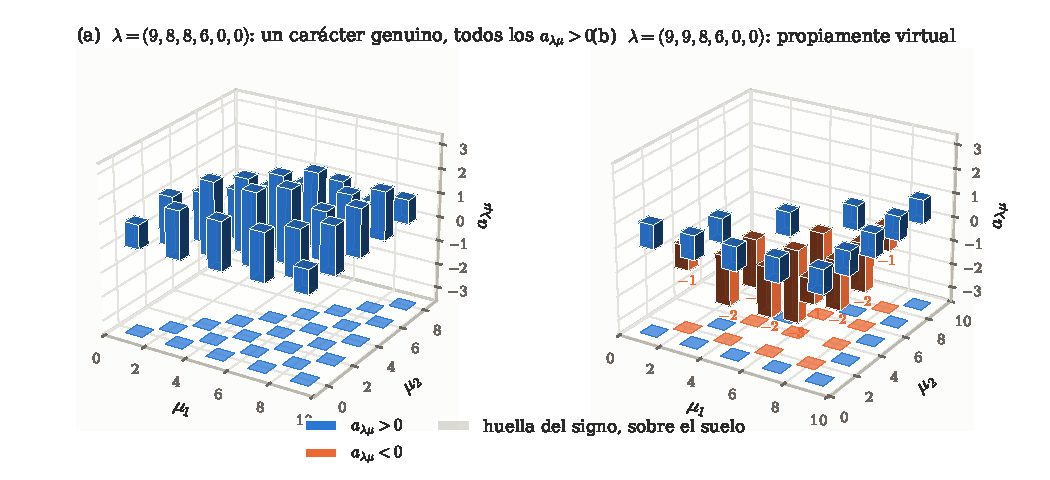
\includegraphics[width=\textwidth]{fig_virtual_es.pdf}
\caption{Por qué un solo par recíproco no es lo típico, en $r=2$: la expansión
$\Psi_r(\lambda)=\sum_\mu a_{\lambda\mu}\,sp_\mu(z)$ sobre los pesos dominantes de $Sp(4)$. Las dos
formas difieren en una sola casilla. Para $\lambda=(9,8,8,6,0,0)$ todo $a_{\lambda\mu}$ es positivo:
el objeto es un carácter genuino, como lo es para \emph{toda} $\lambda$ cuando $r=1$, donde el
Teorema \ref{thm:main} lo escribe como producto de tres caracteres de $\mathfrak{sl}_2$. Para
$\lambda=(9,9,8,6,0,0)$ la expansión tiene $12$ coeficientes positivos y $10$ negativos, siendo el más
negativo $-3$: es genuinamente virtual, que es el fenómeno que recoge la Observación
\ref{rem:rankone} y la razón de que un cálculo en el extremo deje de ser un test exacto pasado un
par. Los dos paneles comparten la escala vertical, y los cuadrados planos del suelo repiten el signo
de cada coeficiente, porque un coeficiente $-1$ es invisible al lado de uno $+3$. Calculada por
\texttt{anc/fig\_v2.py}.}
\label{fig:virtual}
\end{figure}

\subsubsection*{El criterio en \texorpdfstring{$t=2$}{t=2}}

\begin{proof}[Demostración del Teorema \ref{conj:crit}]
La implicación de (a) o (b) a $\Psi_r(\lambda)=0$ es el Teorema \ref{thm:zeros}. Para el recíproco,
supóngase $\Psi_r(\lambda)=\Phi_{2,r}(\lambda;z)\equiv0$ y que ninguna clase de residuos módulo $2$
falta en $\beta(\lambda)$, ya que en otro caso se cumple la rama (a) y no hay nada que probar.
Entonces el numerador se anula idénticamente, así que en particular su componente de grado $D_1$ se
anula y $|G|=2$ por el Corolario \ref{cor:uniquegen}.

Por el Teorema \ref{thm:Ggen}(b) hay un empate en el rango $r$ entre las clases $i$ e $i+t/2=i+1$; en
$t=2$ ésas son las dos clases, y ambas están en $\mathcal{E}$, luego $e=2$. (Con $e=1$ todos los
incrementos viven en una sola clase y son distintos dos a dos por el Paso 4, así que no hay empate
posible.) Como $e=2$, ninguna clase es unitaria y $\mathcal{S}=\{\beta_1,\dots,\beta_N\}$ es el
beta-conjunto entero.

Por el Corolario \ref{cor:Ctaugen}, $C=\min\mathcal{S}+\max\mathcal{S}=\beta_N+\beta_1=\tau$ y, como
cambian las dos clases, $g_{\mathrm{com}}=\varnothing$ en \eqref{eq:gcomgen}, de modo que
\eqref{eq:Ssymgen} se lee $\tau-\mathcal{S}=\mathcal{S}$: el beta-conjunto es simétrico respecto de
$C$, es decir
\[
  \beta_j+\beta_{N+1-j}=C\qquad\text{para todo }j .
\]
Sustituyendo $\beta_j=\lambda_j+N-j$ esto se convierte en $\lambda_j+\lambda_{N+1-j}=C-N+1=:w$ para
todo $j$, que es la auto-complementariedad de anchura $w=\lambda_1+\lambda_N$. Finalmente, el
Corolario \ref{cor:Ctaugen} dice que las dos soluciones de $2\kappa\equiv C\pmod2$ son las dos
clases, lo que ocurre exactamente cuando $C$ es par; y $C=w+N-1$ con $N=2r+2$ par, así que $C$ par es
exactamente $w$ impar. Luego $\lambda$ es auto-complementaria de anchura impar: la rama (b).
\end{proof}

\begin{remark}
En $t=2$ la congruencia \eqref{eq:congrgen} es vacua --- todo incremento es par --- y $|G|\le2$ vale
por la razón más débil de que sólo existen dos clases. Lo que \emph{no} es vacuo en $t=2$ es que
$\tau$ sea par, y se usa dos veces: prohíbe el emparejamiento cruzado en la Proposición
\ref{prop:centregen}, y \emph{es} la paridad que se convierte en la rama (b).
\end{remark}

\begin{remark}[\emph{genuino} no quiere decir \emph{irreducible}]
En la Observación \ref{rem:rankone}, \emph{$\pm$ un carácter genuino} significa una combinación
\emph{no negativa} de irreducibles, no uno solo. No es uno solo: ya
$s_{(2)}(1,-1,z,z^{-1})=z^{2}+2+z^{-2}=sp_{(2)}+sp_{(0)}$. En $t=2$, $r=1$ el Teorema
\ref{thm:main} da un producto de tres caracteres de $\mathfrak{sl}_2$, y un producto de caracteres es
un carácter --- ésa es toda la afirmación. A partir de $r=2$ aparecen coeficientes negativos y no
existe ninguna representación, que es lo que quiere decir \emph{genuinamente virtual}; el Cuadro
\ref{tab:virtual} cuenta las dos cosas y la Figura \ref{fig:virtual} dibuja una de cada.
\end{remark}

\begin{table}[!ht]
\centering\small
\caption{Genuino frente a genuinamente virtual, sobre todas las $\lambda$ con $\lambda_1$ hasta la
cota indicada. La expansión es $\Psi_r(\lambda)=\sum_\mu a_{\lambda\mu}\,sp_\mu(z)$; \emph{un signo}
quiere decir que todos los $a_{\lambda\mu}$ tienen el mismo signo, de modo que $\pm\Psi_r$ es un
carácter, y \emph{mezclado} quiere decir que es genuinamente virtual. En $r=1$ la columna de mezclados
está vacía, como fuerza el Teorema \ref{thm:main}; no lo está para ningún $r\ge2$ al que lleguemos.
Calculada por \texttt{anc/fig\_v2.py}.}
\label{tab:virtual}
\begin{tabular}{@{}lrrrr@{}}
\toprule
 & \multicolumn{1}{c}{formas} & \multicolumn{1}{c}{$\Psi_r=0$} & \multicolumn{1}{c}{un signo}
 & \multicolumn{1}{c}{mezclado} \\
\midrule
\rowcolor{hband} $r=1$, $\lambda_1\le14$ & $3060$ & $352$ & $2708$ & \textcolor{hproved}{$\mathbf{0}$} \\
$r=2$, $\lambda_1\le8$  & $3003$ & $78$ & $2531$ & \textcolor{hverif}{$\mathbf{394}$} \\
$r=3$, $\lambda_1\le5$  & $1287$ & $27$ & $1008$ & \textcolor{hverif}{$\mathbf{252}$} \\
$r=4$, $\lambda_1\le2$  & $66$   & $2$  & $58$   & \textcolor{hverif}{$\mathbf{6}$} \\
\bottomrule
\end{tabular}
\end{table}

\begin{remark}[dónde vive el alfabeto]
Para $r=1$ el alfabeto $(1,-1,z,\bar z)$ de \eqref{eq:psir} es literalmente la lista de valores
propios de una matriz de la componente no identidad $O(4)^{-}$, tabulada como tal por Hanany y
Kalveks \cite[Tabla 7]{HK16}, que además registran la caída de rango
$[\mathrm{vec}]_{O(2n)^{-}}\cong[\mathrm{vec}]_{O(2)^{-}}\oplus[\mathrm{fund}]_{C_{n-1}}$ para la
representación \emph{vectorial}. Así que $\Psi_r$ es un carácter de $GL(2r+2)$ evaluado en esa
componente, y el plegado $D_{r+1}\to C_r$ es la razón de que aparezca un grupo simpléctico; no lo
usamos más que para situar el objeto, ya que para una $\lambda$ cualquiera la restricción es una
combinación con coeficientes enteros de caracteres simplécticos, y no uno solo.
\end{remark}

\section{Verificación}\label{sec:verif}

Todos los enunciados anteriores se comprobaron numéricamente, con tres implementaciones por rutas de
código distintas: una en aritmética de Laurent exacta, otra una evaluación del bialternante escrita
desde cero a partir de los enunciados, y una tercera en Sage, que no comparte con las otras dos ni
una línea de código ni una biblioteca. Los rangos y recuentos se recogen aquí una sola vez.

% longtable y no tabular: con un tabular esta tabla es una caja indivisible, y LaTeX la empuja
% entera a la pagina siguiente dejando la de la cabecera de seccion casi vacia.  longtable parte por
% paginas y repite la cabecera, que es lo que una tabla de cuarenta filas necesita.
% \raggedright en las dos primeras: justificadas, una columna estrecha estira los espacios y deja
% "t <= 7, |lambda| <=" con huecos enormes.  La tercera va \raggedleft porque son cifras.
\begingroup\footnotesize\setlength{\tabcolsep}{4.0pt}
% Anchuras algo menores que en la edicion inglesa: el castellano es mas largo por palabra y con las
% de alla la tabla se salia 4 pt.  Se miden en el PDF, no en el log.
\begin{longtable}{@{}>{\raggedright\arraybackslash}p{0.352\linewidth}%
                  >{\raggedright\arraybackslash}p{0.222\linewidth}%
                  >{\raggedleft\arraybackslash}p{0.272\linewidth}@{\hspace{4pt}}l@{}}
\toprule
enunciado & rango & resultado & estado\\
\midrule
\endfirsthead
\multicolumn{4}{@{}l}{\footnotesize\itshape Verificación, continuación}\\[1pt]
\toprule
enunciado & rango & resultado & estado\\
\midrule
\endhead
\midrule
\multicolumn{4}{r@{}}{\footnotesize\itshape sigue en la página siguiente}\\
\endfoot
\bottomrule
\endlastfoot
Teor. \ref{thm:main}, signo incluido & $t\le7$, $|\lambda|\le14,\dots,10$ &
$959$ exactos, $476$ ceros, $0$ fallos & \stproved\\
\quad lo mismo, una implementación escrita desde el enunciado & $t\le6$, $|\lambda|\le12,\dots,9$ &
$749$ formas, $0$ fallos; el señuelo del signo falla $35/133$ & \stproved\\
Lema \ref{lem:L1} & $t\le6$ & $454$ menores no nulos & \stproved\\
Lema \ref{lem:L4} & $t\le7$ & $724/724$ & \stproved\\
Proposición \ref{prop:quotient} & $t\le7$, $|\lambda|\le19$ & $2970/2970$ & \stproved\\
Prop. \ref{rem:lattice} (lugar concéntrico) & $t\le9$, $|\lambda|\le16$ & $1331/1331$;
$0$ con $t$ impar, $43$ con par & \stproved\\
Prop. \ref{rem:sign} (forma corta del signo) & $t\le8$, $|\lambda|\le14$ & $1496/1496$;
pasos de la prueba, $0$ fallos & \stproved\\
\quad la ley de desplazamiento \eqref{eq:shift} y su signo & $t\le7$, $|\lambda|\le12$ &
$826$ formas, $0$ fallos & \stproved\\
Prop. \ref{prop:minimal} (el multiconjunto separa) & $d_i\le60$; $t\le5$, $|\lambda|\le16$ &
$75640$ invariantes, $0$ colisiones & \stproved\\
\quad lo mismo, en los dos sentidos, desde el enunciado & $t\le5$, $|\lambda|\le14,\dots,11$ &
$676$ formas, $0$ colisiones; señuelo $104$ & \stproved\\
Prop. \ref{prop:fibrelattice} (el retículo) & $t\le5$, $|\lambda|\le14,12,10,10$ &
$84$, $35$, $20$, $14$ fibras, en ambos sentidos & \stproved\\
Cor. \ref{cor:fibregf} (función generatriz) & mismo rango &
$153/153$; denominador erróneo $101$ & \stproved\\
Observación \ref{rem:signsees} (el signo ve los $m_i$) & $t\le4$ &
$107/107$, $43/62$, $26/36$ & \stverif\\
Lema \ref{lem:single} & $t\le7$, $|\lambda|\le16$ & $2113/2113$ & \stproved\\
Teor. \ref{thm:extra} & $t\le12$, $\lambda_1\le33$ & $119+21$, ninguna más & \stproved\\
\quad el signo es $+1$, \eqref{eq:extrainv} & $t\le14$ par; núcleos $t\le10$ &
$28$ extra $+$ $219$ núcleos, todos $+1$ & \stproved\\
Proposición \ref{prop:rect} & $t=2$, $r\le4$, $c\le60$ & $240/240$ & \stproved\\
Cor. \ref{cor:enum} contra enumeración directa & $t\le5$ & $14/14$; cajas $16/16$ &
\stproved\\
Prop. \ref{rem:involution} (las rachas alternan) & $t=2$, $|\lambda|\le14$, $\le4$ filas &
$4823$ menores; $217$ pares, $0$ fallos & \stproved\\
(D3), (D4) de la \S\ref{sec:sharp} & $t\le6$, $|\lambda|\le10$ &
$600$ / $383$ / $200$ de $600$ & \stverif\\
\midrule
\rowcolor{hband} Teor. \ref{conj:crit}, el criterio, todo $r$ & --- & prueba, \S\ref{sec:rigidity} & \stproved\\
\rowcolor{hband} \quad lo mismo, leído sobre $O(N)$, Cor.~\ref{cor:dettwist} & --- &
reformulación, \S\ref{sec:conv} & \stproved\\
\rowcolor{hband} \quad Teor. \ref{thm:PvW}, el input externo & --- & \cite{PvW} & \stext\\
\rowcolor{hband} \quad Teorema \ref{thm:Ggen}, $|G|\le2$ & $t\le10$, $r\le3$ & voraz contra fuerza bruta, $0/4049$ & \stproved\\
\rowcolor{hband} \quad Prop.~\ref{prop:A1gen}, los extremos & $t\le10$, $r\le3$ & $2522$ formas, $0$ fallos & \stproved\\
\rowcolor{hband} \quad \quad la hipótesis hace falta & mismo & $414$ formas fallan sin ella & \stproved\\
\rowcolor{hband} \quad las identidades mostradas, \S\S\ref{sec:extremal}--\ref{sec:rigidity} & $t=2$, $r\le3$ & $11$ identidades, $0$ fallos & \stverif\\
\rowcolor{hband} Lema \ref{lem:step}, movimiento de columna, toda clase & $t\le6$, $r\le3$ &
$285\,600/285\,600$; señuelo de un término $149\,652$ & \stproved\\
\rowcolor{hband} Teor. \ref{thm:suff}, la dirección suficiente & $t\le8$, $r\le4$ &
$438$ formas, $0$ fallos; \eqref{eq:wrefl} $438/438$ & \stproved\\
\rowcolor{hband} Conj. \ref{conj:general}, ambas direcciones & $t\le12$, $r\le4$ &
$190\,443$ formas, $24$ configuraciones, $0$ fallos & \stverif\\
\rowcolor{hband} \quad lo mismo, evaluación independiente & $t\le8$, $r\le4$ &
$43\,010$ formas, $409$ ceros, $0$ fallos & \stverif\\
\rowcolor{hband} \quad lo mismo otra vez, en Sage & $t\le8$, $r\le3$ &
$12\,937$ formas, $131$ ceros, $0$ fallos & \stverif\\
\rowcolor{hband} \quad contra los Teoremas \ref{thm:main} y \ref{conj:crit} & $r=1$; $t=2$ &
$9913$ y $29\,508$ formas, $0$ discrepancias & \stproved\\
\rowcolor{hband} \quad el señuelo que lee $\beta$ en vez de $\mathcal{S}$ & mismo &
falla en $24$ de $24$ y en $14$ de $14$ & \stproved\\
\midrule
\rowcolor{hband} Teor. \ref{conj:crit}, ambas direcciones, comprobación directa & $r\le3$, $|\lambda|\le28,26,22$ &
$9961$ formas, $318$ ceros, $0$ fallos & \stproved\\
\rowcolor{hband} \quad rama (a), Teor.~\ref{thm:zeros} & $r\le3$, $|\lambda|\le15$ &
$16/16$ & \stproved\\
\rowcolor{hband} \quad rama (b), Teor.~\ref{thm:zeros} & $r\le3$ & $24/24$ & \stproved\\
\rowcolor{hband} \quad control de anchura par para (b) & $r\le3$ & $56/56$ no nulos & \stproved\\
\rowcolor{hband} \quad recíproco en $r=1$, Teor.~\ref{thm:r1} & $\beta_1\le25$ &
$14950$ conjuntos beta, $0$ fallos & \stproved\\
\rowcolor{hband} \quad recíproco, $\ell(\lambda)\le N/2$, Teor.~\ref{thm:stable} & $r\le3$ &
$372/372$ testigos & \stproved\\
\rowcolor{hband} \quad el testigo aislante, Prop.~\ref{conj:iso} & $r=2$, $|\lambda|\le14$ &
$227$ testigos, $11$ de residuo & \stproved\\
\rowcolor{hband} \quad lo mismo en $r=3$ & $r=3$, $|\lambda|\le13$ &
$149$ testigos, $0$ de residuo & \stproved\\
\midrule
Identidad \eqref{eq:compl} & $r\le2$ & $474/474$ & \stproved\\
Identidad \eqref{eq:docagne}, y $\deg_{c_\ast}S_n=n-1$ & $b\le31$ & $496/496$; $39/39$ &
\stproved\\
Lema \ref{lem:AtoSp}, la reducción de la \S\ref{sec:unstable} & $r\le3$, $|\nu|\le8$ &
identidad $0$ fallos; plegados $0$ fallos & \stproved\\
\quad la reducción, llevada a cabo & $r\le2$ & $236$ etiquetas, $0$ sin resolver & \stproved\\
\eqref{eq:Cmu} contra el objeto exacto & $r\le2$, ambos rangos & $184$ formas, $0$ fallos &
\stverif\\
\end{longtable}
\endgroup

\noindent El bloque sombreado es el Teorema \ref{thm:zeros} leído de arriba abajo: las dos ramas
suficientes están demostradas para todo $r$, el recíproco está demostrado para un par y, para todo
$r$, dentro del rango de Littlewood; y la línea que solía quedar ---el recíproco para $r\ge2$ fuera
de ese rango y más allá de la franja $|\lambda|\le2r+2$ que resuelve el Lema \ref{lem:nonstd}---
es el Teorema \ref{conj:crit}, demostrado en la \S\ref{sec:rigidity} por un argumento que no entra
en el rango de Littlewood. Por eso el bloque lleva ya \stproved\ en todas sus filas, con una en
\stext\ para el apoyo ajeno del que depende. La fila que registra lo que hace y lo que no hace el
certificado que propusimos se queda, y lleva \stproved\ porque la Proposición \ref{conj:iso} es un
contraejemplo y los contraejemplos son demostraciones; lo que acota ahora es una vía, no el
enunciado. Las filas por debajo del bloque son las identidades y la reducción sobre
las que se apoya la sección. En la columna, \stproved\ significa que aquí se da una demostración o se
cita, y \stverif\ que el enunciado se comprueba de forma exhaustiva sobre el rango indicado y no se
demuestra.

\noindent La fila de (D3), (D4) es la que más importa del primer grupo: la identidad se cumple en los
$600$ casos para \eqref{eq:object} y falla en $217$ y $400$ de ellos para los dos alfabetos
deformados, de modo que el contraste es capaz de fallar. En el segundo grupo, el control de anchura
par cumple el mismo papel para el Teorema \ref{thm:zeros}: $56$ formas autocomplementarias de anchura
par, ninguna de las cuales se anula, así que la hipótesis de paridad trabaja en lugar de decorar. Una
auditoría aparte reconstruye todo el segundo grupo desde las definiciones en una sola pasada, con
independencia de los guiones que los produjeron: $3414$ comprobaciones, $0$ fallos. Una segunda toma
las \emph{fórmulas mostradas} en vez de los recuentos ---el Teorema \ref{thm:LR}, la lectura por
intervalos \eqref{eq:intervals}, los Lemas \ref{lem:L2} y \ref{lem:L5}, la partición
\eqref{eq:threestep}, la complementación \eqref{eq:compl}, d'Ocagne \eqref{eq:docagne} y la
advertencia escalar \eqref{eq:scalar}--- y evalúa ambos miembros en puntos numéricos desde las
definiciones, sin usar ni las formas cerradas de este artículo ni los guiones que sostienen la
tabla: $3297$ evaluaciones sobre nueve fórmulas mostradas, $0$ fallos. Los guiones son
material auxiliar de este artículo, y también lo es la salida guardada de cada uno, de modo que todo
recuento de la tabla anterior puede localizarse en una ejecución archivada en lugar de aceptarse por
confianza.

%======================================================================
\section{Problemas abiertos}\label{sec:open}

La Figura \ref{fig:map} sitúa lo que sigue frente a lo que el artículo demuestra y lo que toma
prestado; los problemas de abajo son las cajas que deja abiertas.

\begin{figure}[!ht]
\centering
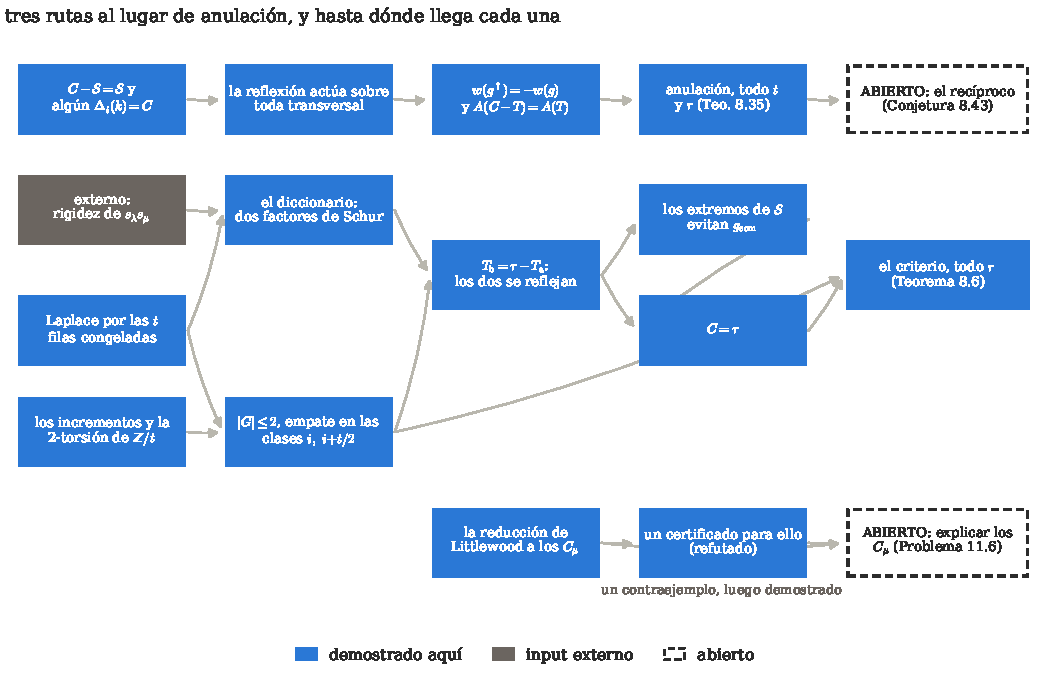
\includegraphics[width=\textwidth]{fig_map_es.pdf}
\caption{Sobre qué se apoya el criterio de la \S\ref{sec:zeros} y qué queda. Las cajas son
enunciados y las flechas dependencias; el color es la columna de estado de la \S\ref{sec:verif} ---
relleno lo demostrado aquí, gris el único apoyo ajeno, discontinuo lo abierto. La rama de arriba es
el argumento extremal de las \S\S\ref{sec:extremal} y \ref{sec:rigidity}; la de abajo es la
reducción de Littlewood, cuyo certificado refuta la Proposición \ref{conj:iso} ---un contraejemplo,
o sea una demostración---, de modo que la rama de abajo ya no toca el criterio sino la cuestión
aparte de explicar los $C_\mu$, que es el Problema \ref{prob:instrument}. Los enunciados van por
nombre y no por número, para que la figura no pueda desfasarse cuando la numeración lo haga.
Calculada por \texttt{anc/fig\_proof.py}.}
\label{fig:map}
\end{figure}

\begin{problem}[los otros tipos clásicos]\label{prob:types}
Todo lo anterior es de tipo $A$. ¿Qué hacen $sp_\lambda(\zt,z,\zb)$, $so_\lambda(\zt,z,\zb)$ y
$o_\lambda(\zt,z,\zb)$? Las factorizaciones de raíces de la unidad se llevaron del tipo $A$ a los
tipos $B$, $C$, $D$ con un argumento uniforme en \cite{AK22} y a los caracteres universales en
\cite{Alb23}; las filas congeladas del bialternante son las mismas en todos los tipos, de modo que el
Lema \ref{lem:L1} y el recuento de exceso dos deberían sobrevivir palabra por palabra, mientras que
el colapso, los Lemas \ref{lem:L4} y \ref{lem:L5}, habría que rehacerlo una vez por tipo. El alfabeto
\eqref{eq:object} es ya un elemento del toro de $O(t+2)$, de modo que los otros tipos no son la misma
función en un punto nuevo sino objetos nuevos, y elegir los correctos es cuestión de criterio dentro
de un programa que no hemos construido nosotros. Sí hemos medido, y lo damos como medición y nada
más. Desarrollando los caracteres universales de Koike--Terada en la base de Schur y evaluando
término a término con el Teorema \ref{thm:main}, sobre $|\lambda|\le12$ para $t\le3$ y
$|\lambda|\le10$ para $t=4,5$, la fracción de formas con $\ell(\lambda)\ge2$ en las que el valor se
anula es netamente mayor para $o_\lambda$ en la componente no identidad que en la identidad ---el
$83.8\%$ con $t=2$ frente al $41.8\%$ con $t=3$, y el $58.8\%$ con $t=4$ frente al $42.1\%$ con
$t=5$---, con $sp_\lambda$ en medio y el caso de Schur el más bajo. El efecto es real y sigue a la
componente, que es lo que cabría esperar de una cancelación entre asociados; pero es cuantitativo y
no le hemos encontrado ley que cubra la tabla entera. Un primer intento de ley, que $o_\lambda$ se
anule para todo
$\ell(\lambda)\ge2$ cuando $t$ es par, es falso: se leyó de una muestra y el barrido sistemático lo
refuta.

La columna $t=2$ de esa comparación es el único caso que sí tiene ley, y es el Lema
\ref{lem:AtoSp}: allí el alfabeto es \eqref{eq:psir} con $r=1$, de modo que $o_\nu$ es igual a
$sp_\nu(z)$, un carácter simpléctico de \emph{rango uno}. Ése se anula idénticamente para
$\ell(\nu)=2$ --- las $36$ formas del rango, sin excepción --- y se pliega para $\ell(\nu)>2$, que es
la razón de que la cifra de $t=2$ sea la que se sale. Lo que queda sin ley es $t$ impar, donde el
alfabeto no tiene la forma \eqref{eq:psir} y el lema no se aplica.

La columna de $sp_\lambda$ en $t=2$, en cambio, sí tiene respuesta, y explica la asimetría de la
tabla en lugar de añadirle una fila. Adjuntar esas mismas dos letras a un carácter universal
\emph{simpléctico} no lo colapsa. Sobre $|\nu|\le8$,
\begin{equation}\label{eq:spbranch}
sp_\nu(W,1,-1)\;=\;\sum_{\gamma\subseteq\nu}c_{\nu/\gamma}\;sp_\gamma(W),
\end{equation}
donde el coeficiente depende de $\nu$ y $\gamma$ solo a través de la forma sesgada $\nu/\gamma$
---$247$ coeficientes sobre $74$ formas sesgadas distintas, sin un solo choque--- y toma únicamente
los valores $0$ y $\pm1$, anulándose siempre que $|\nu/\gamma|$ es impar. Esa es la forma que produce
una regla de ramificación para funciones simplécticas universales, y tales reglas existen
\cite{JJLW24}. Leído contra ella, el Lema \ref{lem:AtoSp} dice que para $o_\nu$ los coeficientes
correspondientes se concentran en $\gamma=\nu$: las dos letras colapsan el carácter ortogonal a un
único carácter simpléctico, y dejan el simpléctico repartido por todo el intervalo bajo $\nu$. La
asimetría de la medición es eso, y no un artefacto de los rangos. Lo que no hemos hecho es
identificar $c_{\nu/\gamma}$, que \eqref{eq:spbranch} convierte en una pregunta sobre caracteres
simplécticos universales sesgados en $(1,-1)$ y en nada más.

La tercera columna se resiste a la misma vía, y por una razón estructural y no accidental. Lo que
resuelve las otras dos es que adjuntar una letra es el mapa de anillos $p_k\mapsto p_k+c^k$, de modo
que $\iota_{1}$ y $\iota_{-1}$ actúan sobre $\Lambda$ y componen. La identidad que traería $so$ al
cuadro, $so_\nu(X)=o_\nu(X,\bar X,1,0,\dots)$ de \cite[(2.13)]{AK25}, relaciona ambos sobre un
alfabeto \emph{duplicado}, y una duplicación no es una adjunción: los $\iota$ no llegan. Así que la
columna $so$ no es una laguna de esfuerzo sino de mecanismo, y la dejamos enunciada como tal.
\end{problem}

\begin{problem}[una Verschiebung que vea un par recíproco]\label{prob:versch}
El operador $\varphi_t$ no tiene nada que decir sobre una letra fuera de una $\zeta$-órbita, que es
la razón estructural de que el Teorema \ref{thm:main} no sea corolario de nada de esa línea, y la
razón de que nuestra demostración descienda al alternante. ¿Existe un operador sobre caracteres
universales, o una factorización de $\varphi_t$ a través de un álgebra mayor, que actúe sobre
alfabetos de la forma (unión de $\zeta$-órbitas) $\cup$ (pares recíprocos)? Por la \S\ref{sec:sharp},
un operador así decidiría (D1) y (D2) de una vez. La discusión de allí sugiere una forma
cuantitativa.

Lo que vuelve bien planteada la pregunta, y no vaga, es que cada mitad tiene ya un formalismo, y no
son el mismo. Las $\zeta$-órbitas son territorio de $\varphi_t$, en la formulación de Albion
\cite{Alb23}. Los alfabetos cerrados por inversión son territorio de las funciones simplécticas y
ortogonales universales, que admiten realizaciones por operadores de vértice de las que se siguen sus
reglas de ramificación \cite{JJLW24}. Nuestro alfabeto es uno de cada, y el Lema \ref{lem:AtoSp} es
el único sitio donde ambos se encuentran: allí la $\zeta$-órbita es $\{1,-1\}$, lo bastante pequeña
como para que adjuntarla sea un par de mapas de letra y no un operador. No conocemos nada que actúe
sobre las dos mitades a la vez, y la pregunta es si los dos formalismos componen.
\end{problem}

\begin{proposition}[el rango es el invariante equivocado]\label{conj:rank}
Sea $A=\zt\cup B$ con $B$ cerrado bajo inversión y disjunto de $\zt$, y sea $\rho(B)$ el rango del
subgrupo de $\CC^{\times}$ generado por $B$. Entonces $\rho(B)=1$ no implica que $s_\lambda(A)$ sea
un producto de caracteres. En $t=2$ y $B=\{z,z^{-1},z^{2},z^{-2}\}$, que tiene $\rho(B)=1$, el valor
en $\lambda=(2)$ tiene una raíz fuera de la circunferencia unidad, y por tanto no admite tal
factorización; lo mismo ocurre con $B=\{z,z^{-1},z^{3},z^{-3}\}$.
\end{proposition}

\begin{proof}
Un producto de caracteres $\chi_k(z)=(z^{k+1}-z^{-k-1})/(z-z^{-1})$ tiene todas sus raíces en la
circunferencia unidad, así que basta exhibir una raíz fuera de ella. Para
$B=\{z,z^{-1},z^{2},z^{-2}\}$ y $\lambda=(2)$ el valor es
$z^{-4}+z^{-3}+z^{-2}+z^{-1}+3+z+z^{2}+z^{3}+z^{4}$. El polinomio de Laurent es invariante bajo
$z\mapsto z^{-1}$, de modo que escribiendo $x=z+z^{-1}$ y usando $z^{k}+z^{-k}\in\ZZ[x]$ queda
\[
x^{4}+x^{3}-3x^{2}-2x+3\;=\;(x-1)\bigl(x^{3}+2x^{2}-x-3\bigr).
\]
La cúbica tiene discriminante
$18\cdot2\cdot(-1)(-3)-4\cdot2^{3}(-3)+2^{2}(-1)^{2}-4(-1)^{3}-27\cdot(-3)^{2}=-31<0$, luego dos de
sus raíces no son reales. Si $|z|=1$, entonces $x=z+z^{-1}=2\cos\theta$ es real; así que para una
raíz no real $x_0$, ninguna de las dos raíces de $z^{2}-x_0z+1=0$ está en la circunferencia unidad, y
las dos son raíces del valor. Luego la factorización es imposible, y el enunciado es exacto y no
numérico.

Sobre $|\lambda|\le8$ el mismo fenómeno ocurre en $17$ de las $62$ formas no nulas, y con
$B=\{z,z^{-1},z^{3},z^{-3}\}$ en $18$; en el mismo rango, $B=\{z,z^{-1}\}$ tiene todas sus raíces en
la circunferencia sin excepción, como exige el Teorema \ref{thm:main}.
\end{proof}

Lo que el rango no ve es cuántas direcciones libres tiene $B$. Un solo par recíproco es una
dirección; $\{z,z^{-1},z^{2},z^{-2}\}$ genera un grupo de rango uno y son dos, y las dos se ven entre
sí. Así que el invariante sobre el que conjeturar no es $\rho(B)$ sino el número de letras
independientes, y con esa lectura el enunciado pasa a ser el que la \S\ref{sec:sharp} ya hace por
otros medios:

\begin{conjecture}[una sola dirección libre]\label{conj:rank2}
Sea $B$ cerrado bajo inversión y disjunto de $\zt$, como en la Proposición \ref{conj:rank}. Entonces
$s_\lambda(\zt\cup B)$ es cero o un producto de caracteres, para toda $\lambda$, si y solo si $B$ es
un único par recíproco. (La alternativa no es decoración: por el Corolario \ref{cor:zero} el valor sí
se anula para alguna $\lambda$ ya con un par, y $0$ no es un producto de caracteres.)
\end{conjecture}

La evidencia a su favor es el Teorema \ref{thm:main} en un sentido y (D1)--(D4) junto con la
Proposición \ref{conj:rank} en el otro: agrandar $B$ destruye el producto, suba o no suba el rango la
ampliación. No tenemos demostración ni mecanismo propuesto, y es precisamente el enunciado que un
argumento del estilo de $\varphi_t$ debería producir.

Esa hipótesis es bajo la que se enuncia la conjetura, y es también la que una forma general tendría
que soltar. El cierre por inversión de $B$ es suficiente
en la evidencia anterior, pero no es necesario para que haya producto. Escribamos $w=-iy$. El segundo
bloque del alfabeto $\{1,-1,y,-y^{-1}\}$ no es cerrado por inversión y, sin embargo,
\begin{equation}\label{eq:scalar}
s_\lambda\big(1,-1,y,-y^{-1}\big)\;=\;i^{\,|\lambda|}\,s_\lambda\big(-i,\,i,\,w,\,w^{-1}\big),
\end{equation}
y el alfabeto de la derecha sí lo es. La hipótesis que llevaría una forma proyectivamente invariante
no es, por tanto, el cierre por inversión de $B$, sino que $A$ sea un múltiplo
escalar de un conjunto cerrado por inversión. Una clase lateral $\zeta\zt$ es ella misma cerrada por
inversión exactamente cuando $\zeta^{2}=\pm1$, que es donde (D3) rompe y donde no.

\begin{problem}[el instrumento para el segundo par]\label{prob:instrument}
La Sección \ref{sec:zeros} reduce la anulación en $r\ge2$ a un enunciado sobre los coeficientes
$C_\mu$ de \eqref{eq:Cmu}, que son sumas con signo de coeficientes de Littlewood. Ese enunciado ya
no es lo que falta: el Teorema \ref{conj:crit} resuelve la anulación, por el argumento extremal de
la \S\ref{sec:rigidity}, que no se cruza con ningún $C_\mu$. Lo que la reducción pide ahora no es
una demostración sino una \emph{explicación} ---por qué se cancelan esas sumas con signo, en los
propios términos de Littlewood--- y sigue sin haber certificado, pues el que propusimos falla por la
Proposición \ref{conj:iso}. Un problema que era un hueco pasa a ser una pregunta por una segunda
demostración, que es mejor problema y más pequeño. El Lema \ref{lem:AtoSp} resuelve la otra mitad de la reducción --- qué
son los valores $o_\nu(A)$ --- y la resuelve simplécticamente: las dos lecturas del alfabeto
concuerdan porque son la misma lectura, pues el álgebra órbita de $D_{r+1}$ es $C_r$ y no la
subálgebra fija $B_r$. Lo que no toca son los coeficientes. Kumari y Stokke \cite{KS26} han dado
reglas de Murnaghan--Nakayama para funciones de Schur simplécticas, ortogonales y ortosimplécticas;
por el Lema \ref{lem:AtoSp} la pertinente aquí es la simpléctica \cite[Teorema 3.4]{KS26}, y no la
ortogonal par \cite[Teorema 3.10]{KS26}. ¿Calcula su recursión los
$C_\mu$? Su regla arrastra un tercer sumando más allá de añadir y quitar tiras de borde, y es el que
ellas mismas señalan como complicado; el \cite[Corolario 3.5]{KS26} muestra que desaparece en cuanto
$\mu_n+1\ge r$, de modo que es un fenómeno de formas poco profundas. Una forma anterior de este
problema preguntaba si ese sumando es el que da cuenta del fallo de la regla de Littlewood fuera de su
rango; el Lema \ref{lem:AtoSp} responde que no, pues el fallo lo llevan las reglas de modificación
simplécticas, que actúan sobre las etiquetas y no dentro de la recursión. Lo que queda son los
coeficientes, y lo que no hemos intentado es si esa recursión los calcula.

Hay un segundo instrumento, y es el que probaríamos primero. Las reglas de ramificación de Frohmader
\cite{Frohmader} calculan $\mathrm{mult}(\pi^{\nu}_{O_n},\pi^{\lambda}_{GL_n})$ como
$\sum_{\mu}c^{\lambda}_{\mu\nu}(O_n)$ sobre las particiones $\mu$ de filas pares, sin restricción de
rango estable y sin regla de modificación. Nuestros $C_\mu$ de \eqref{eq:Cmu} son sumas con signo de
exactamente las multiplicidades que esas reglas calculan, ensambladas por la involución asociada
$\nu\mapsto\nu^{*}$. Así que la pregunta se vuelve concreta: ¿es $C_\mu(\lambda)=0$, en las dos
ramas, una identidad entre coeficientes de Littlewood--Richardson generalizados que las condiciones
de bandera hagan visible? Ésa es una pregunta sobre tablas, que es la forma en la que nos gustaría
verla contestada.
\end{problem}

\begin{problem}[el lugar adicional, en general]\label{prob:extralocus}
¿Tiene el Teorema \ref{thm:extra} análogo para $sp$, $so$ y $o$? Más en general, ¿para qué
especializaciones de las variables libres adquiere el criterio \eqref{eq:AK53} soluciones
adicionales, y puede leerse siempre el lugar adicional en el núcleo de la especialización actuando
sobre el espacio generado por los caracteres universales, como sugiere la Observación
\ref{rem:why}? Si cada tipo adquiere una familia indexada por un elemento de orden dos del retículo
de residuos, el principio es real.

La pregunta necesita fijar la parte libre, y por una razón computada: la familia extra es un
fenómeno del alfabeto \emph{mínimo}. Añádase un segundo par recíproco y desaparece ---sobre
$t=3,4,5,6$ y $|\lambda|\le14$ el lugar pasa a ser exactamente los $t$-núcleos, para el tipo $s$
tanto como para $sp$ y $o$, mientras que con un solo par el tipo $s$ tiene los dos extras del Teorema
\ref{thm:extra} en $t=4$ y uno en $t=6$. (El segundo par se prueba en $z_2=z_1^{2}$, una
especialización, que solo puede crear coincidencias y no eliminarlas, de modo que un recuento de cero
ahí es un recuento de cero.) El análogo para otro tipo hay que buscarlo, por tanto, en la parte libre
mínima \emph{de ese tipo}, una letra de cada clase; comparar tipos con partes libres de tamaños
distintos mide la parte libre, que es lo que hizo nuestro primer intento.

El núcleo es lo que hay que mirar, pero su \emph{presencia} no decide el lugar; lo decide su
tamaño. Dos partes libres del mismo tamaño pueden colapsar ambas la independencia y comportarse de
manera muy distinta. En el lugar recíproco $s_\mu(z,\zb)=\chi_{\mu_1-\mu_2}(z)$ conserva una
graduación, y el lugar extra es la única familia del Teorema \ref{thm:extra}. Sustitúyase el par
por la $\zeta_2$-órbita $(z,-z)$, donde $s_\mu(z,-z)=z^{|\mu|}s_\mu(1,-1)$ conserva sólo $|\mu|$ y
un signo, y sobre $\ell(\lambda)\le2$ el criterio adquiere $28$ soluciones más en $t=2$ y $186$ en
$t=8$, en ninguna familia que sepamos nombrar. El control es el par libre $(z,w)$, que no tiene
núcleo y devuelve los $t$-núcleos y nada más para todo $t\le8$ ---que es \eqref{eq:AK53} misma, de
modo que el control es su teorema y no una medición nuestra. Así que el par recíproco es la
especialización colapsante de núcleo \emph{mínimo}, y
eso, y no la mera existencia de un núcleo, es lo que hace que su lugar extra sea una sola familia.
\end{problem}

\begin{problem}[las fibras, refinadas por el signo]\label{prob:fibres}
El Corolario \ref{cor:fibregf} describe la fibra de la terna de intervalos, y solo eso. El
invariante es $I_t=(d_1,d_2,d_3,\varepsilon_\lambda)$, y el signo corta cada rama todavía más. Su
corte no es contabilidad, y no es ocioso: por la Observación \ref{rem:signsees} el signo ve las
$t-2$ direcciones que la terna no ve, desde $t=3$ ---constante en $(m_i)$ a $v$ fijo en los $107$
huecos de $t=2$, pero solo en $43$ de $62$ en $t=3$ y $26$ de $36$ en $t=4$. ¿Cuál es la
restricción de $\varepsilon_\lambda$ a una rama? La obstrucción para leerla de
\eqref{eq:fibrelattice} está a la vista en \eqref{eq:sign}: $\inv(b_S)$ es un estadístico de la
palabra beta entera, y las coordenadas del retículo parten esa palabra en dos clases distinguidas y
$t-2$ letras libres, de modo que una regla tendría que volver a montar lo que la biyección separa.

Van con él dos huecos menores. La misma descripción para el perfil de tamaño tres debería ser la
misma contabilidad con una clase de tres en lugar de dos de dos; no la hemos escrito. El perfil
degenerado es otra pregunta, porque allí la fibra es el lugar de anulación entero de $\Phi_t$, que
el Corolario \ref{cor:zero} y la Proposición \ref{rem:lattice} describen por otros medios.
\end{problem}

\begin{problem}[un tamiz que conserva un parámetro]\label{prob:sieving}
En $t=2$ el Corolario \ref{cor:enum} es un recuento con signo de $\mathrm{SSYT}(\lambda,4)$, y un
recuento con signo de orden dos es lo que calcula el fenómeno $q=-1$ de Stembridge \cite{Ste94}:
sobre un conjunto que lleva una involución, el valor en $-1$ cuenta los puntos fijos. Ese es el caso
$\#C=2$ del fenómeno de tamiz cíclico de Reiner, Stanton y White \cite{RSW04}, cuyo Teorema 4.3
evalúa la especialización principal $s_\lambda(1,q,\dots,q^{k-1})$ en una raíz primitiva $d$-ésima
de la unidad en términos del $d$-núcleo y el $d$-cociente de $\lambda$ ---los dos invariantes que
sostienen también el Teorema \ref{thm:main}--- y que Lee y Oh \cite{LO22} han extendido después a
formas sesgadas. Toda evaluación de esa línea es en un \emph{número}, como un enunciado de tamiz
exige: allí el alfabeto es la progresión geométrica $1,q,\dots,q^{k-1}$ especializada en una raíz de
la unidad, no una órbita llana, y no queda nada libre. La nuestra no es de esa clase ---el par
recíproco conserva $z$, y \eqref{eq:main} es una fórmula de producto en él. ¿Hay una acción cíclica
sobre $\mathrm{SSYT}(\lambda,t+2)$, y un $q$-análogo de $\Phi_t$, cuyo valor en una raíz $t$-ésima
de la unidad cuente puntos fijos refinados por $m_{t+1}-m_{t+2}$? El caso $\#C=2$ es por donde mirar
primero, y allí la involución que un enunciado así necesitaría ya existe: la \S\ref{sec:enum} la
ensambla.

Planteada así, la pregunta tiene nombre. Los enunciados de cribado que conservan un estadístico
adicional se estudian por derecho propio ---Ahlbach y Swanson \cite{AS18} refinan el cribado cíclico
sobre palabras fijando el tipo de descenso cíclico junto al índice mayor--- y la forma de dos
variables, en la que una segunda graduación lleva una segunda acción, es el cribado \emph{bicíclico}
de Barcelo, Reiner y Stanton \cite{BRS08}. Sobre tablas semiestándar en particular, Oh y Park
\cite{OP19} construyen una acción cíclica a partir de la estructura de cristal cuyo polinomio de
cribado es $q^{-\kappa(\lambda)}s_\lambda(1,q,\dots,q^{n-1})$ ---la mitad congelada de nuestro
alfabeto, evaluada exactamente como un enunciado de cribado exige--- y obtienen un enunciado
bicíclico para los ganchos; Alexandersson, Kantarc\i{} O\u{g}uz y Linusson \cite{AKL21} hacen lo
mismo bajo promoción para varias familias de formas. Ninguno de ellos conserva una variable
\emph{libre}, que es lo que \eqref{eq:object} sí hace y lo que vuelve distinta la pregunta de aquí,
pero entre todos dicen qué aspecto debería tener una respuesta. La forma afilada es entonces: ¿lleva
cada fibra de peso $z$ fijo de $\mathrm{SSYT}(\lambda,t+2)$ un cribado cíclico propio?

La mitad de existencia de la pregunta es decidible sin exhibir la acción. Alexandersson y Amini
\cite{AA19} dan un criterio necesario y suficiente para que exista una acción cíclica que realice un
polinomio de tamiz dado: para todo $d\mid t$, el valor en $\omega^d$ debe ser
$\sum_{j\mid d}j\,c_j$ con todos los $c_j$ enteros no negativos, y los $c_j$ ---los números de
órbitas de cada tamaño--- se calculan entonces por triangularidad. Aplicado al candidato que sugiere
el propio alfabeto, $F(q,z)=s_\lambda(1,q,\dots,q^{t-1},z,z^{-1})$, cuya graduación en $z$ es ya el
refinamiento que se pide, el criterio se cumple para casi toda pieza graduada en los rangos que
alcanzamos; pero también para un refinamiento deliberadamente equivocado, graduando por
$m_{t+1}+m_{t+2}$, que pasa al mismo ritmo. A esos tamaños el criterio no discrimina, y damos el
intento como evidencia en ninguna de las dos direcciones.
\end{problem}

Una laguna más estrecha queda registrada donde surge y no aquí, con la misma forma que los problemas
anteriores y el mismo significado ---algo que querríamos saber y no hemos resuelto---: la involución
de la \S\ref{sec:enum} queda ensamblada en $t=2$ y en ningún otro sitio, porque la Proposición
\ref{rem:involution} es un enunciado sobre una palabra y esa palabra es la de $t=2$. La
distinción que mantenemos en todo el texto es entre una \emph{conjetura}, que es un enunciado que
creemos y hemos testado, y un \emph{problema}, que no es una afirmación en absoluto.

Tomados juntos, los problemas dicen dónde creemos que el objeto deja de ser nuestro. La evaluación
está completa y el alfabeto es mínimo, así que lo que queda no es más de lo mismo: es si los dos
formalismos que se reparten las dos mitades de \eqref{eq:object} componen, si un enunciado de tamiz
puede conservar una variable, y qué hacen los coeficientes $C_\mu$ una vez retirado el certificado
que habíamos propuesto para ellos. De los tres, el último es el que el artículo necesita y el primero
es el que preferiríamos ver contestado.

Conviene cerrar donde empezamos. La introducción nombró dos razones para que la evaluación de un
carácter colapse ---que el alfabeto sea una órbita, y que sea cerrado por inversión--- y observó que
ningún alfabeto había llevado una de cada. Éste sí, y las dos razones se comportan en él de manera
muy distinta. La mitad de la órbita está agotada: el Teorema \ref{thm:main} la evalúa en forma
cerrada para todo $t$, y el Teorema \ref{thm:extra} muestra que, dentro del problema de independencia
para formas de dos filas, exactamente una familia más se comporta así. La mitad de la inversión no lo
está: la letra $-1$ lleva el alfabeto a la componente no identidad de un grupo ortogonal, y eso ha
bastado para decir bastante sobre \emph{dónde} se anula el carácter ---el Teorema \ref{conj:crit} lo
resuelve en $t=2$ para cualquier número de pares, y el Teorema \ref{thm:suff} da una implicación para
todo $t$ y todo $r$---, pero no nos ha dicho qué \emph{es} el carácter allí para más de un par, y la
otra implicación es la Conjetura \ref{conj:general}. El valor no deja nunca de ser un valor de
carácter: es $s_\lambda$ evaluado en un elemento del toro en todo momento. Lo que deja de valer,
pasado un par, es que su expansión simpléctica plegada sea siempre un carácter genuino: a partir de
dos pares aparecen ejemplos genuinamente virtuales. Eso es un enunciado sobre la expansión, no sobre
el objeto. Lo que el artículo entrega es más pequeño que cualquiera de las dos mitades y más portátil: una
forma cerrada que lleva su signo, lo que convierte a esta familia en un caso de prueba para cualquier
implementación de caracteres torcidos o universales; un test de anulación que cuesta dos restas sobre
el conjunto beta; y una enumeración en la que el parámetro sigue libre. Quien
busque el alfabeto siguiente habrá de buscar el que deje la segunda razón tan completa como aquí ha
quedado la primera; a la vista de la \S\ref{sec:sharp}, no lo encontrará añadiendo letras a éste.

\subsection*{Agradecimientos}
Este artículo existe porque Arvind Ayyer preguntó si el caso de rango uno se generaliza a $t$
arbitrario con la variable libre simbólica. La pregunta era mejor que la nota que la provocó. Le
agradecemos tanto la pregunta como la correspondencia que siguió. La Observación \ref{rem:core} existe
porque Nishu Kumari preguntó si la condición $n_i(\lambda)=0$ podía formularse en términos del
$t$-núcleo; también confirmó la lectura de \cite[Teorema 5.3]{AK25} de la \S\ref{sec:independence}, y
fue un apunte suyo el que nos envió a \cite[\S3]{AK25}, donde esperaba el Lema \ref{lem:AtoSp}; se lo
agradecemos. La involución de la
\S\ref{sec:enum} está montada a partir de tres lemas de su tesis \cite{KumariThesis}, y en ese
sentido también es suya.

Hay una tercera deuda, y es con una herramienta y no con una conversación. La prueba del Teorema
\ref{thm:suff} depende de poder reflejar un conjunto beta dentro de un determinante sin desarrollar
nada, y la manera de hacerlo --- escalar cada fila por una potencia para mandar $x_i$ a $\bar x_i$ y
luego invertir un bloque de columnas --- es la maniobra de Ayyer y Behrend \cite[\S3]{AB19}, usada del
lado de las raíces de la unidad por Albion \cite{Alb23,Alb25}. La adoptamos porque es a todas luces
el instrumento adecuado para un alfabeto cerrado por inversión, y la mantuvimos porque resultó ser
más robusta que el contexto para el que se escribió: en ningún momento usa que la reflexión se
aplique al alfabeto entero, así que funciona igual sobre una parte de él. Todo lo que la
\S\ref{sec:zeros} dice sobre $t\ge4$ se apoya en eso.

\subsection*{Código, datos y declaración}
Todo cálculo citado en este artículo lo realiza un script con nombre, distribuido como fichero
adjunto, y todo número citado lo reproduce una ejecución archivada de alguno de ellos; la
\S\ref{sec:verif} tabula qué script responde por qué afirmación. Los mismos scripts y la misma salida
están también en \url{https://github.com/karlesmarin/schur-orbit-and-reciprocal-pair}. Se ha usado IA generativa (Claude,
Anthropic) como asistente de investigación durante todo el trabajo: para la búsqueda bibliográfica,
para escribir y comprobar el código adjunto, y sobre la prosa. Las matemáticas, y la responsabilidad
sobre ellas, son del autor.

%======================================================================
\begin{thebibliography}{AAAA}

\bibitem[FG86]{FG86} A.~Federgruen y H.~Groenevelt, \emph{The greedy procedure for resource
allocation problems: necessary and sufficient conditions for optimality}, Oper. Res. \textbf{34}
(1986), no.~6, 909--918.

\bibitem[HK16]{HK16} A.~Hanany y R.~Kalveks, \emph{Quiver theories for moduli spaces of classical
group nilpotent orbits}, arXiv:1601.04020.

\bibitem[IK88]{IK88} T.~Ibaraki y N.~Katoh, \emph{Resource Allocation Problems: Algorithmic
Approaches}, MIT Press, Cambridge MA, 1988.

\bibitem[PvW08]{PvW} K.~Purbhoo y S.~van Willigenburg, \emph{On tensor products of polynomial
representations}, Canad. Math. Bull. \textbf{51} (2008), no.~4, 584--592; arXiv:0706.3251.

\bibitem[Raj04]{Rajan} C.~S.~Rajan, \emph{Unique decomposition of tensor products of irreducible
representations of simple algebraic groups}, Ann. of Math. (2) \textbf{160} (2004), no.~2, 683--704.

\bibitem[RGST05]{TropCramer} J.~Richter-Gebert, B.~Sturmfels y T.~Theobald, \emph{First steps in
tropical geometry}, en: Idempotent Mathematics and Mathematical Physics, Contemp. Math. \textbf{377},
Amer. Math. Soc., 2005, pp.~289--317.


\bibitem[Alb23]{Alb23} S.~P.~Albion, \emph{Universal characters twisted by roots of unity},
Algebraic Combinatorics \textbf{6} (2023), 1653--1676; arXiv:2212.07343.

\bibitem[Alb25]{Alb25} S.~P.~Albion, \emph{Character factorisations, $z$-asymmetric partitions and
plethysm}, en prensa en Combinatorial Theory; arXiv:2501.18520.

\bibitem[AS18]{AS18} C.~Ahlbach y J.~P.~Swanson, \emph{Refined cyclic sieving on words for the
major index statistic}, European J. Combin. \textbf{73} (2018), 37--60; arXiv:1706.08631.

\bibitem[BRS08]{BRS08} H.~Barcelo, V.~Reiner y D.~Stanton, \emph{Bimahonian distributions},
J. London Math. Soc. (2) \textbf{77} (2008), 627--646; arXiv:math/0703479.

\bibitem[OP19]{OP19} Y.-T.~Oh y E.~Park, \emph{Crystals, semistandard tableaux and cyclic sieving
phenomenon}, Electron. J. Combin. \textbf{26} (2019), no.~4, \#P4.39; arXiv:1906.07420.

\bibitem[AKL21]{AKL21} P.~Alexandersson, E.~Kantarc\i{} O\u{g}uz y S.~Linusson, \emph{Promotion and
cyclic sieving on families of SSYT}, Ark. Mat. \textbf{59} (2021), 247--274; arXiv:2007.10478.

\bibitem[AA19]{AA19} P.~Alexandersson y N.~Amini, \emph{The cone of cyclic sieving
phenomena}, Discrete Math. \textbf{342} (2019), n.º~6, 1581--1601; arXiv:1804.01447.

\bibitem[AB19]{AB19} A.~Ayyer y R.~E.~Behrend, \emph{Factorization theorems for classical group
characters, with applications to alternating sign matrices and plane partitions}, J. Combin. Theory
Ser.~A \textbf{165} (2019), 78--105; arXiv:1804.04514.

\bibitem[AK22]{AK22} A.~Ayyer y N.~Kumari, \emph{Factorization of classical characters twisted by
roots of unity}, J. Algebra \textbf{609} (2022), 437--483; arXiv:2109.11310.

\bibitem[AK25]{AK25} A.~Ayyer y N.~Kumari, \emph{Further results for classical and universal
characters twisted by roots of unity}, J. Algebraic Combin. \textbf{63} (2026), Paper No.~2, 32 pp.;
arXiv:2501.00275.

\bibitem[CK09]{CK09} M.~Ciucu y C.~Krattenthaler, \emph{A factorization theorem for classical
group characters, with applications to plane partitions and rhombus tilings}, in: Advances in
Combinatorial Mathematics, Springer, Berlin, 2009.

\bibitem[GKS90]{GKS90} F.~Garvan, D.~Kim y D.~Stanton, \emph{Cranks and $t$-cores},
Invent. Math. \textbf{101} (1990), no.~1, 1--18.

\bibitem[HI24]{HI24} M.~Hidaka y M.~Itoh, \emph{The Schur polynomials in all primitive $n$th roots
of unity}, J. Combin. Theory Ser.~A \textbf{218} (2026), Paper No.~106107; arXiv:2403.10817.

\bibitem[Jan73]{Jantzen} J.~C.~Jantzen, \emph{Darstellungen halbeinfacher algebraischer Gruppen},
Bonner Math. Schriften \textbf{67} (1973).

\bibitem[Kar22]{Kar22} C.~Karmakar, \emph{Character factorizations for representations of
$GL(n,\CC)$}, arXiv:2210.03544.

\bibitem[Kar24]{Kar24} C.~Karmakar, \emph{Character values at elements of order $2$},
Proc. Indian Acad. Sci. Math. Sci. \textbf{135} (2025), no.~2, Paper No.~41; arXiv:2412.17324.

\bibitem[Mar26]{Mar26} C.~Mar\'in, \emph{Schur functions at $(1,-1,t,t^{-1})$: a closed form on the
non-identity component of $O(4)$}, preprint, 2026; \texttt{doi:10.5281/zenodo.21463000}.

\bibitem[JJLW24]{JJLW24} Z.~Jin, N.~Jing, Z.~Li y D.~Wang, \emph{Universal symplectic/orthogonal
functions and general branching rules}, arXiv:2209.00767.

\bibitem[KLP09]{KLP} S.~Kumar, G.~Lusztig y D.~Prasad, \emph{Characters of simply-laced
nonconnected groups versus characters of nonsimply-laced connected groups}, Contemp. Math.
\textbf{478} (2009), 99--101; arXiv:math/0701615.

\bibitem[KT99]{KT99} A.~Knutson y T.~Tao, \emph{The honeycomb model of $GL_n(\CC)$ tensor
products I: proof of the saturation conjecture}, J. Amer. Math. Soc. \textbf{12} (1999), no.~4,
1055--1090.

\bibitem[Kum24]{Kum24} N.~Kumari, \emph{Factorization of classical characters twisted by roots of
unity: II}, J. Pure Appl. Algebra \textbf{228} (2024), no.~11, 107714; arXiv:2212.12477.

\bibitem[KumT]{KumariThesis} N.~Kumari, \emph{Characters of classical groups twisted by roots of
unity}, tesis doctoral, Indian Institute of Science, Bangalore, 2023.

\bibitem[Lec09]{Lec09} C.~Lecouvey, \emph{Parabolic Kazhdan--Lusztig polynomials, plethysm and
generalized Hall--Littlewood functions for classical types}, European J. Combin. \textbf{30} (2009),
no.~1, 157--191.

\bibitem[LR34]{LR34} D.~E.~Littlewood y A.~R.~Richardson, \emph{Immanants of some special
matrices}, Q. J. Math. \textbf{os-5} (1934), no.~1, 269--282.

\bibitem[LLT97]{LLT97} A.~Lascoux, B.~Leclerc y J.-Y.~Thibon, \emph{Ribbon tableaux,
Hall--Littlewood functions, quantum affine algebras and unipotent varieties}, J. Math. Phys.
\textbf{38} (1997), no.~2, 1041--1068.

\bibitem[LO22]{LO22} S.-Y.~Lee and Y.-T.~Oh, \emph{Skew Schur polynomials and cyclic sieving
phenomenon}, Electron. J. Combin. \textbf{29} (2022), no.~4, Paper 4.6; arXiv:2112.12394.

\bibitem[Mac95]{Mac95} I.~G.~Macdonald, \emph{Symmetric Functions and Hall Polynomials}, second
edition, Oxford University Press, 1995.

\bibitem[RSW04]{RSW04} V.~Reiner, D.~Stanton y D.~White, \emph{The cyclic sieving phenomenon},
J. Combin. Theory Ser. A \textbf{108} (2004), no.~1, 17--50.

\bibitem[Ste94]{Ste94} J.~R.~Stembridge, \emph{On minuscule representations, plane partitions and
involutions in complex Lie groups}, Duke Math. J. \textbf{73} (1994), no.~2, 469--490.

\bibitem[Oka98]{Oka98} S.~Okada, \emph{Applications of minor summation formulas to
rectangular-shaped representations of classical groups}, J. Algebra \textbf{205} (1998), no.~2,
337--367.

\bibitem[Pra16]{Pra16} D.~Prasad, \emph{A character relationship on $GL_n(\CC)$}, Israel J. Math.
\textbf{211} (2016), no.~1, 257--270.

\bibitem[AF20]{AF20} A.~Ayyer e I.~Fischer, \emph{Bijective proofs of skew Schur polynomial
factorizations}, J. Combin. Theory Ser.~A \textbf{174} (2020), 105241; arXiv:1905.05226.

\bibitem[Doc]{Doc} Para el nombre y la familia de identidades que lo rodea (Cassini, Catalan,
d'Ocagne, Vajda) véase p.\,ej.\ M.~Bunder y J.~Tonien, \emph{Cassini, d'Ocagne and Vajda identities
for $n$-step Fibonacci numbers}, arXiv:2201.06269.

\bibitem[Eis07]{Eis07} T.~Eisenk\"olbl, \emph{A Schur function identity related to the
$(-1)$-enumeration of self-complementary plane partitions}, J. Combin. Theory Ser.~A \textbf{115}
(2008), 199--212; arXiv:math/0602401.

\bibitem[FJKW05]{FJKW05} B.~Fauser, P.~D.~Jarvis, R.~C.~King y B.~G.~Wybourne, \emph{New branching
rules induced by plethysm}, J. Phys. A \textbf{39} (2006), 2611--2655; arXiv:math-ph/0508034.

\bibitem[Gav99]{Gav99} F.~Gavarini, \emph{A Brauer algebra-theoretic proof of Littlewood's
restriction rules}, J. Algebra \textbf{212} (1999), 240--271.

\bibitem[EW04]{EW04} T.~J.~Enright y J.~F.~Willenbring, \emph{Hilbert series, Howe duality and
branching for classical groups}, Ann. of Math. \textbf{159} (2004), 337--375.

\bibitem[New51]{New51} M.~J.~Newell, \emph{Modification rules for the orthogonal and symplectic
groups}, Proc. Roy. Irish Acad. Sect. A \textbf{54} (1951), 153--163.

\bibitem[Sun90]{Sun90} S.~Sundaram, \emph{Tableaux in the representation theory of the classical Lie
groups}, en \emph{Invariant Theory and Tableaux} (Minneapolis, MN, 1988), IMA Vol. Math. Appl.
\textbf{19}, 191--225, Springer-Verlag, Nueva York, 1990.

\bibitem[IOTZ06]{IOTZ06} M.~Ishikawa, S.~Okada, H.~Tagawa y J.~Zeng, \emph{Generalizations of
Cauchy's determinant and Schur's Pfaffian}, Adv. in Appl. Math. \textbf{36} (2006), 251--287.

\bibitem[Fro25]{Frohmader} A.~Frohmader, \emph{Graded multiplicities in the Kostant--Rallis
setting}, arXiv:2312.11295.

\bibitem[Kra05]{KratADCC} C.~Krattenthaler, \emph{Advanced determinant calculus: a complement},
Linear Algebra Appl. \textbf{411} (2005), 68--166; arXiv:math/0503507.

\bibitem[Kin71]{King71} R.~C.~King, \emph{Modification rules and products of irreducible
representations of the unitary, orthogonal, and symplectic groups}, J. Math. Phys. \textbf{12}
(1971), 1588--1598.

\bibitem[KT87]{KT87} K.~Koike e I.~Terada, \emph{Young-diagrammatic methods for the representation
theory of the classical groups of type $B_n$, $C_n$, $D_n$}, J. Algebra \textbf{107} (1987),
466--511.

\bibitem[KS26]{KS26} N.~Kumari y A.~Stokke, \emph{Murnaghan--Nakayama rules for symplectic,
orthogonal and orthosymplectic Schur functions}, Discrete Math. \textbf{349} (2026), no.~2, Paper
No.~114741; arXiv:2411.11447.

\bibitem[Kup02]{Kup02} G.~Kuperberg, \emph{Symmetry classes of alternating-sign matrices under one
roof}, Ann. of Math. (2) \textbf{156} (2002), 835--866.

\bibitem[Lit50]{Lit50} D.~E.~Littlewood, \emph{The Theory of Group Characters and Matrix
Representations of Groups}, 2.\textsuperscript{a} ed., Oxford University Press, 1950.

\bibitem[SK23]{SK23} V.~Sathish Kumar, \emph{Flagged skew Schur polynomials twisted by roots of
unity}, arXiv:2306.10289.

\bibitem[Sta86]{Sta86} R.~P.~Stanley, \emph{Symmetries of plane partitions}, J. Combin. Theory
Ser.~A \textbf{43} (1986), 103--113.

\end{thebibliography}

\end{document}
